\documentclass[10pt]{article}

  \usepackage{pgfplots}
\pgfplotsset{compat=newest}
%% the following commands are needed for some matlab2tikz features
\usetikzlibrary{plotmarks}
\usetikzlibrary{arrows.meta}
\usepgfplotslibrary{patchplots}
\usepackage{grffile}
\usepackage{amsmath}


%\usepackage{fullpage}
\usepackage[top=1in, bottom=1in, left=0.8in, right=1in]{geometry}
\usepackage{multicol}
%\usepackage{wrapfig}
%\usepackage{listings}
\usepackage{caption}
\usepackage{subcaption}
\usepackage{hyperref}
\usepackage{xcolor}
%\usepackage{soul}
\usepackage{graphicx}
\usepackage[pdf]{pstricks}

\definecolor{lightblue}{rgb}{.80,.9,1}
\newcommand{\hl}[1]
    {\par\colorbox{lightblue}{\parbox{\linewidth}{#1}}}

\newcommand{\defn}{\stackrel{\textrm{\scriptsize def}}{=}}

\setlength{\columnsep}{0.1pc}

\title{Generalised Serre-Green-Naghdi Model}
%\author{Christopher Zoppou -- \texttt{christopher.zoppou@anu.edu.au}, Dimitrios Mitsotakis -- \texttt{dmitsot@gmail.com}, Stephen Roberts -- \texttt{stephen.roberts@anu.edu.au}, Jordan Pitt}

% TIME ON EVERY PAGE AS WELL AS THE FILE NAME
\usepackage{fancyhdr}
\usepackage{currfile}
\usepackage[us,12hr]{datetime} % `us' makes \today behave as usual in TeX/LaTeX
\fancypagestyle{plain}{
\fancyhf{}
\rfoot{\emph{\footnotesize \textcopyright  Serre Notes by C. Zoppou, D. Mitsatakis and S. Roberts.}
 \\ File Name: {\currfilename} \\ Date: {\ddmmyyyydate\today} at \currenttime}
\lfoot{Page \thepage}
\renewcommand{\headrulewidth}{0pt}}
\pagestyle{plain}

\begin{document}

\maketitle

\vspace{-0.3in}
\noindent
\rule{\linewidth}{0.4pt}

%-------------------------------------------------
%\section{Introduction}
%-------------------------------------------------



%-------------------------------------------------
\section{gSGN - generalised Serre-Green-Naghdi equations}
%-------------------------------------------------
Clamond and Dutykh\cite{Clamond-Dutykh-2018-237} derived the following generalised version of the Serre-Green-Naghdi equations:

\begin{subequations}
	\begin{gather}
	\dfrac{\partial h}{\partial t} + \dfrac{\partial (uh)}{\partial x} = 0
	\label{eq:gSGNh}
	\end{gather}
	\begin{gather}
	\dfrac{\partial (uh)}{\partial t} + \dfrac{\partial }{\partial x} \left( u^2h + \dfrac{gh^2}{2} + \frac{1}{3} h^2 \Gamma \right)= 0
	\label{eq:gSGNuh}
	\end{gather}
	\begin{multline}
	\dfrac{\partial}{\partial t}\left[\frac{1}{2}hu^2 + \dfrac{1}{2}\left(1 + \frac{3}{2}\beta_1\right) h^3 \dfrac{\partial u}{\partial x}\dfrac{\partial u}{\partial x} + \frac{1}{2}gh^2\left(1 + \frac{1}{2}\beta_2 \dfrac{\partial h}{\partial x} \dfrac{\partial h}{\partial x}\right) \right] \\
	\dfrac{\partial}{\partial x}\left[uh\left(\frac{1}{2}u^2 + \dfrac{1}{2}\left(1 + \frac{3}{2}\beta_1\right)h^2\dfrac{\partial u}{\partial x}\dfrac{\partial u}{\partial x} + gh\left(1 + \frac{1}{4}\beta_2\dfrac{\partial h}{\partial x}\dfrac{\partial h}{\partial x} \right)   + \frac{1}{3} h\Gamma  \right) + \frac{1}{2}\beta_2 g h^3\dfrac{\partial h}{\partial x}\dfrac{\partial u}{\partial x} \right]
	=0
	\label{eq:gSGNE}
	\end{multline}
	where
	\begin{equation}
	\Gamma = \left(1 + \frac{3}{2}\beta_1\right)h \left[\frac{\partial u}{\partial x}\frac{\partial u}{\partial x} - \frac{\partial^2 u}{\partial x \partial t} - u\frac{\partial^2 u}{\partial x^2}\right] - \frac{3}{2} \beta_2 g\left[h \frac{\partial^2 h}{\partial x^2} + \frac{1}{2} \frac{\partial h}{\partial x}\frac{\partial h}{\partial x} \right]
	\end{equation}
	\label{eq:gSGN}
\end{subequations}

These equations have the same order of approximation in the lagrangian density (dispersion properties?) when $\beta_1 = \beta_2$. The interesting thing about the equations though, is that we will conserve mass, momentum and energy for all values of $\beta_j$. 

From these equations the SWWE, the Serre equations and the regularised SWWE \cite{Clamond-Dutykh-2018-237} can be recovered for certain values of $\beta_1$ and $\beta_2$. 

%\begin{itemize}
%	\item When $\beta_1 = 2\epsilon -\frac{2}{3}$ and $\beta_2 = 2 \epsilon$ we get the regularised Saint Venant equations of \cite{Clamond-Dutykh-2018-237}. Which admit the SWWE when $\epsilon = 0$. 
%	\item When $\beta_1 = \beta_2$ we get the improved Serre-Green-Naghdi equations, which when $\beta_1 =\beta_2 = 0$ are the Serre-Green-Naghdi equations. 
%\end{itemize}

\begin{table}
	\centering
	\begin{tabular}{c | c | c}
		Resulting Equations &$\beta_1$ & $\beta_2$  \\
		\hline 
		Serre Equations & $0$ & $0$ \\
		SWWE Equations & $-\dfrac{2}{3}$ & $0$ \\
		Regularised SWWE Equations & free variable & $\beta_1 + \dfrac{2}{3}$  \\
		Improved Dispersion Serre Equations & free variable & $\beta_1$
	\end{tabular}
	\caption{Showing various combinations of $\beta$ values and equivalent equations}
\end{table}

%-------------------------------------------------
\subsection{Alternative Conservative Form of the gSGN}
%-------------------------------------------------

A major difficulty with solving the SGN is that the dispersive terms contain a mixed spatial-temporal derivative term which is difficult to handle numerically. This mixed derivative term can be rewritten  so that the Serre equations can be expressed in conservation law form, with the water depth and a new quantity as conservative variables. This reformulation allows standard techniques for solving conservation laws to be applied to the Serre equations, even though the Serre equations are neither hyperbolic nor parabolic.

Consider the Serre equations written for a horizontal bed. The flux term in the momentum equation, \eqref{eq:gSGNuh} contains a mixed spatial and temporal derivative term which is difficult to treat numerically. It is possible to replace this term  by a combination of spatial and temporal derivative terms by making the following observation
\begin{multline}
\dfrac{\partial^2}{\partial x \partial t} \left ( \frac{1}{3}\left(1 + \frac{3}{2} \beta_1\right) h^3 \dfrac{\partial u}{\partial x} \right ) =   \frac{1}{3}\left(1 + \frac{3}{2} \beta_1\right) \dfrac{\partial }{\partial t} \left ( 3h^2 \dfrac{\partial h}{\partial x} \dfrac{\partial u}{\partial x} + h^3 \dfrac{\partial^2 u}{\partial x^2} \right ) \\=  \frac{1}{3}\left(1 + \frac{3}{2} \beta_1\right)
\dfrac{\partial }{\partial x} \left ( 3 h^2 \dfrac{\partial h}{\partial t} \dfrac{\partial u}{\partial x} + h^3 \dfrac{\partial^2 u}{\partial x \partial t} \right ).
\end{multline}
Rearranging and making use of the continuity equation, \eqref{eq:gSGNh} the momentum equation, \eqref{eq:gSGNuh} becomes
\begin{multline}
\dfrac{\partial }{\partial t} \left ( u h -  \frac{1}{3}\left(1 + \frac{3}{2} \beta_1\right) \dfrac{\partial}{\partial x} \left [h^3 \dfrac{\partial u}{\partial x}  \right ] \right ) \\ + \dfrac{\partial}{\partial x} \left ( u\left[uh - \frac{1}{3}\left(1 + \frac{3}{2} \beta_1\right) \dfrac{\partial }{\partial x} \left [ h^3 \dfrac{\partial u}{\partial x} \right ]\right] + \dfrac{gh^2}{2} - \frac{2}{3}\left(1 + \frac{3}{2} \beta_1\right) h^3\dfrac{\partial u}{\partial x}\dfrac{\partial u}{\partial x}  - \frac{1}{2} \beta_2 g h^2 \left[h\frac{\partial^2 h}{\partial x^2} + \frac{1}{2}\frac{\partial h}{\partial x}\frac{\partial h}{\partial x}\right]\right ) = 0.
\end{multline}
The momentum equation can be written in conservation law form as
\begin{gather}\label{eq:G_momentum}
\dfrac{\partial G }{\partial t}  + \dfrac{\partial}{\partial x} \left ( uG + \dfrac{gh^2}{2} - \frac{2}{3}\left(1 + \frac{3}{2} \beta_1\right) h^3\dfrac{\partial u}{\partial x}\dfrac{\partial u}{\partial x}  - \frac{1}{2} \beta_2 g h^2  \left[h\frac{\partial^2 h}{\partial x^2} + \frac{1}{2}\frac{\partial h}{\partial x}\frac{\partial h}{\partial x}\right]\right ) = 0.
\end{gather}
where a new conserved quantity, $G$ is given by
\begin{gather*}
G = uh - \frac{1}{3}\left(1 + \frac{3}{2} \beta_1\right) \dfrac{\partial }{\partial x} \left ( h^3 \dfrac{\partial u}{\partial x} \right ).
\end{gather*}
This expands the conserved variable introduced by \cite{Clamond-Dutykh-2018-237}, as well as in the Serre equations []. 

Thus we have the following conservation equations

\begin{subequations}
\begin{gather}
\dfrac{\partial h}{\partial t} + \dfrac{\partial (uh)}{\partial x} = 0
\label{eq:gSGN_Gh}
\end{gather}
\begin{gather}
\dfrac{\partial G }{\partial t}  + \dfrac{\partial}{\partial x} \left ( uG + \dfrac{gh^2}{2} - \frac{2}{3}\left(1 + \frac{3}{2} \beta_1\right) h^3\dfrac{\partial u}{\partial x}\dfrac{\partial u}{\partial x}  - \frac{1}{2} \beta_2 g h^2  \left[h\frac{\partial^2 h}{\partial x^2} + \frac{1}{2}\frac{\partial h}{\partial x}\frac{\partial h}{\partial x}\right]\right ) = 0.
\label{eq:gSGN_GG}
\end{gather}
with
\begin{gather}\label{eq:G_divergent}
G = uh - \frac{1}{3}\left(1 + \frac{3}{2} \beta_1\right) \dfrac{\partial }{\partial x} \left ( h^3 \dfrac{\partial u}{\partial x} \right ).
\end{gather}
\end{subequations}

\subsection{Dispersion Relation of Linearised gSGN}

Assuming that
\begin{align*}
h(x,t) &= h_0 + \delta \eta(x,t) + O(\delta^2)\\
u(x,t) &= u_0 + \delta v(x,t) + O(\delta^2)
\end{align*}

By substituting these forms into the linearised Serre equations and neglecting $O(\delta^2)$ terms, we get the linearised regularised Serre equations. We also substitute $\eta_t$ using the mass equation into the momentum equation. 


\begin{subequations}
	\begin{equation}
	\label{eqlinhd}
	(\delta\eta)_t + u_0 (\delta \eta)_x + h_0 (\delta v)_x = 0
	\end{equation}
	\begin{equation}
	\label{eqlinuhd}
	h_0(\delta v)_t + gh_0(\delta \eta)_x + h_0u_0 (\delta v)_x - \frac{1}{3}\left(1 + \frac{3}{2}\beta_1\right) h_0^3(\delta v)_{xxt} - \frac{1}{3}\left(1 + \frac{3}{2}\beta_1\right) h_0^3 u_0 (\delta v)_{xxx} -\frac{g\beta_2}{2}h_0^3 (\delta \eta)_{xxx}  = 0
	\end{equation}
\end{subequations}

We can remove the $\delta$ term, either by removing the common factor, or absorbing it into $\eta$ and $v$ to get

\begin{subequations}
	\begin{equation}
	\label{eqlinh}
	\eta_t + u_0 \eta_x + h_0 v_x = 0
	\end{equation}
	\begin{equation}
	\label{eqlinuh}
	h_0(v)_t + gh_0(\eta)_x + h_0u_0 (v)_x - \frac{1}{3}\left(1 + \frac{3}{2}\beta_1\right) h_0^3(v)_{xxt} - \frac{1}{3}\left(1 + \frac{3}{2}\beta_1\right) h_0^3 u_0 ( v)_{xxx} -\frac{g\beta_2}{2}h_0^3 (\eta)_{xxx}  = 0
	\end{equation}
\end{subequations}

We now assume that $\eta(x,t) = H \exp\left(i (k x - \omega t)\right)$,  $v(x,t) = U \exp\left(i (k x - \omega t)\right)$
\begin{align*}
\eta(x,t) &= H \exp\left(i (k x - \omega t)\right) \\
v(x,t) &= U \exp\left(i (k x - \omega t)\right)
\end{align*}

substituting these into the linearised Serre equation we get

\begin{subequations}
	\begin{equation}
	\label{eqlinhexp}
	\left[H u_0 k - H \omega + U h_0k\right]i \exp\left[i \left(k x - \omega t\right)\right] = 0
	\end{equation}
	\begin{multline}
	\label{eqlinuhexp}
	\bigg[3H \beta_2 g h_0^2 k^3 + 6Hgk - 3U \beta_1 \omega h_0^2 k^2 + 3U\beta_1 h_0^2 k^3 u_0\\ - 2U \omega h_0^2 k^2 - 6U \omega + 2U h_0^2 k^3 u_0 + 6U k u_0\bigg] i \frac{h_0}{6} \exp\left[i \left(k x - \omega t\right)\right] = 0
	\end{multline}
\end{subequations}


This can be written as
\begin{equation}
\begin{bmatrix}
u_0k - \omega & h_0 k \\
3 \beta_2 h_0^2 k^3 + 6k g & -3 \beta_1 \omega h_0^2 k^2 + 3 \beta_1 h_0^2 k^3 u_0 - 2\omega h_0^2 k^2 - 6\omega + 2h_0^2 k^3 u_0 + 6ku_0
\end{bmatrix}
\begin{bmatrix}
H \\ U
\end{bmatrix} = 0
\end{equation}

Which has non-trivial solutons when the determinant is zero. 

The determinant of this matrix is
\begin{equation}
\left(3\beta_1 h_0^2 k^2 + 2h_0^2 k^2 + 6\right)\omega^2 - 2 u_0k \left(3\beta_1 h_0^2 k^2 + 2h_0^2 k^2 + 6\right)\omega  + u_0^2 k^2 \left(3\beta_1 h_0^2 k^2 + 2h_0^2 k^2 + 6\right) - g h_0 k^2 \left(3 \beta_2 h_0^2 k^2 + 6\right)
\end{equation} 

To get non-trivial solution we have

\begin{equation}
\left(3\beta_1 h_0^2 k^2 + 2h_0^2 k^2 + 6\right)\omega^2 - 2 u_0k \left(3\beta_1 h_0^2 k^2 + 2h_0^2 k^2 + 6\right)\omega  + u_0^2 k^2 \left(3\beta_1 h_0^2 k^2 + 2h_0^2 k^2 + 6\right) - g h_0 k^2 \left(3 \beta_2 h_0^2 k^2 + 6\right) = 0
\end{equation} 

\begin{equation}
\omega^2 - 2 u_0k \omega  + u_0^2 k^2 - g h_0 k^2 \dfrac{3 \beta_2 h_0^2 k^2 + 6}{\left(3\beta_1 h_0^2 k^2 + 2h_0^2 k^2 + 6\right)} 
\end{equation} 

Using quadratic equation, or another quadratic polynomial solver we get that

\begin{equation}
\omega^\pm = u_0 k \pm k \sqrt{gh_0} \sqrt{\dfrac{3 \beta_2 h_0^2 k^2 + 6}{\left(3\beta_1 h_0^2 k^2 + 2h_0^2 k^2 + 6\right)} }
\end{equation}

\begin{equation}
\omega^\pm = u_0 k \pm k \sqrt{gh_0} \sqrt{\dfrac{\beta_2 h_0^2 k^2 + 2}{\left(\frac{2}{3} + \beta_1\right) h_0^2 k^2 + 2} }
\end{equation}


Thus we have the following regimes
\begin{itemize}
	\item SWWE wavespeeds (non-dispersive): occurs when $\beta_2 = \frac{2}{3} + \beta_1$ then $\omega^\pm = k\left(u_0\pm \sqrt{gh_0}\right)$ (\cite{Clamond-Dutykh-2018-237}).
	\item Serre wavespeeds - when $\beta_1 = \beta_2 = 0$ - we get $\omega^\pm = k\left(u_0\pm \sqrt{gh_0} \sqrt{\dfrac{3}{3 + h_0^2 k^2}}\right)$
	\item For other values of $\beta_1$ and $\beta_2$ we can vary the wavespeeds, in certain situations this will lead to a better approximation of the linear wavespeed of waves than the Serre equations ( \cite{Clamond-Dutykh-2018-237}), in others it will be worse. We show an example below.
\end{itemize}

Now for the group speed
\begin{equation}
v^\pm_g = \frac{\partial \omega^\pm }{\partial k}= u_0  \pm  \sqrt{gh_0} \sqrt{\dfrac{\beta_2 h_0^2 k^2 + 2}{\left( \left(\frac{2}{3} + \beta_1\right) h_0^2 k^2 + 2\right)} } \pm \dfrac{k\sqrt{gh_0}}{\beta_2 h_0^2 k^2 +2} \left[\sqrt{\dfrac{\beta_2 h_0^2 k^2 + 2}{\left( \left(\frac{2}{3} + \beta_1\right) h_0^2 k^2 + 2\right)} } \left( \beta_2 h_0^2 k - \dfrac{h_0^2 k \left(\beta_1 + \frac{2}{3}\right)\left(\beta_2h_0^2k^2 + 2\right)}{h_0^2 k^2 \left(\beta_1 + \frac{2}{3}\right) + 2} \right)\right]
\end{equation} 

\begin{multline*}
= u_0  \pm  \sqrt{gh_0} \sqrt{\dfrac{\beta_2 h_0^2 k^2 + 2}{\left( \left(\frac{2}{3} + \beta_1\right) h_0^2 k^2 + 2\right)} } \pm \\ \dfrac{k\sqrt{gh_0}}{\beta_2 h_0^2 k^2 +2} \left[\sqrt{\dfrac{\beta_2 h_0^2 k^2 + 2}{\left( \left(\frac{2}{3} + \beta_1\right) h_0^2 k^2 + 2\right)} } \left(  \dfrac{\beta_2 h_0^2 k^2 \left[h_0^2 k^2 \left(\beta_1 + \frac{2}{3}\right) + 2\right] -h_0^2 k \left(\beta_1 + \frac{2}{3}\right)\left(\beta_2h_0^2k^2 + 2\right)}{h_0^2 k^2 \left(\beta_1 + \frac{2}{3}\right) + 2} \right)\right]
\end{multline*} 

\begin{multline*}
= u_0  \pm  \sqrt{gh_0} \sqrt{\dfrac{\beta_2 h_0^2 k^2 + 2}{\left( \left(\frac{2}{3} + \beta_1\right) h_0^2 k^2 + 2\right)} } \pm \\ \dfrac{k\sqrt{gh_0}}{\beta_2 h_0^2 k^2 +2} \left[\sqrt{\dfrac{\beta_2 h_0^2 k^2 + 2}{\left( \left(\frac{2}{3} + \beta_1\right) h_0^2 k^2 + 2\right)} } \left(  \dfrac{  \beta_2 h_0^4 k^3 \left(\beta_1 + \frac{2}{3}\right)  + 2\beta_2 h_0^2 k -h_0^2 k \left(\beta_1 + \frac{2}{3}\right)\left(\beta_2h_0^2k^2 + 2\right)}{h_0^2 k^2 \left(\beta_1 + \frac{2}{3}\right) + 2} \right)\right]
\end{multline*} 

\begin{multline*}
= u_0  \pm  \sqrt{gh_0} \sqrt{\dfrac{\beta_2 h_0^2 k^2 + 2}{\left( \left(\frac{2}{3} + \beta_1\right) h_0^2 k^2 + 2\right)} } \pm \\ \dfrac{k\sqrt{gh_0}}{\beta_2 h_0^2 k^2 +2} \left[\sqrt{\dfrac{\beta_2 h_0^2 k^2 + 2}{\left( \left(\frac{2}{3} + \beta_1\right) h_0^2 k^2 + 2\right)} } \left(  \dfrac{  \beta_2 h_0^4 k^3 \left(\beta_1 + \frac{2}{3}\right)  + 2\beta_2 h_0^2 k -  \beta_2\left(\beta_1 + \frac{2}{3}\right)h_0^4k^3 -    2 h_0^2 k \left(\beta_1 + \frac{2}{3}\right)}{h_0^2 k^2 \left(\beta_1 + \frac{2}{3}\right) + 2} \right)\right]
\end{multline*} 


\begin{multline*}
= u_0  \pm  \sqrt{gh_0} \sqrt{\dfrac{\beta_2 h_0^2 k^2 + 2}{\left( \left(\frac{2}{3} + \beta_1\right) h_0^2 k^2 + 2\right)} } \pm \\ \dfrac{k\sqrt{gh_0}}{\beta_2 h_0^2 k^2 +2} \left[\sqrt{\dfrac{\beta_2 h_0^2 k^2 + 2}{\left( \left(\frac{2}{3} + \beta_1\right) h_0^2 k^2 + 2\right)} } \left(  \dfrac{  2\beta_2 h_0^2 k  -    2 h_0^2 k \left(\beta_1 + \frac{2}{3}\right)}{h_0^2 k^2 \left(\beta_1 + \frac{2}{3}\right) + 2} \right)\right]
\end{multline*} 

\begin{multline*}
= u_0  \pm  \sqrt{gh_0} \sqrt{\dfrac{\beta_2 h_0^2 k^2 + 2}{\left( \left(\frac{2}{3} + \beta_1\right) h_0^2 k^2 + 2\right)} } \pm  2\dfrac{k^2h_0^2\sqrt{gh_0}}{\beta_2 h_0^2 k^2 +2} \left[\sqrt{\dfrac{\beta_2 h_0^2 k^2 + 2}{\left( \left(\frac{2}{3} + \beta_1\right) h_0^2 k^2 + 2\right)} } \left(  \dfrac{\beta_2  -    \beta_1 - \frac{2}{3}}{h_0^2 k^2 \left(\beta_1 + \frac{2}{3}\right) + 2} \right)\right]
\end{multline*} 

\begin{equation*}
= u_0  \pm  \sqrt{gh_0} \sqrt{\dfrac{\beta_2 h_0^2 k^2 + 2}{\left( \left(\frac{2}{3} + \beta_1\right) h_0^2 k^2 + 2\right)} } \left[1 +  \dfrac{\beta_2 - \beta_1 - \frac{2}{3}}{\left(\frac{1}{2}\beta_2 h_0^2 k^2 +1\right)\left( \left(\frac{1}{3} + \beta_1\right) h_0^2 k^2 + 1\right)}\right] 
\end{equation*} 


When $\beta_2 = \frac{2}{3} + \beta_1$ then the group speed is equal to the phase speed of the Shallow Water Wave equations. When $\beta_2 = \beta_1 = 0$ then we get

\begin{equation*}
= u_0  \pm  \sqrt{gh_0} \sqrt{\dfrac{2}{\left( \frac{2}{3} h_0^2 k^2 + 2\right)} } \left[1 + \dfrac{- \frac{1}{3}}{\left( \frac{1}{3} h_0^2 k^2 + 1\right)}\right] 
\end{equation*} 

\begin{equation*}
= u_0  \pm  \sqrt{gh_0} \sqrt{\dfrac{3}{  h_0^2 k^2 + 3} } \left[1 -  \dfrac{1}{ h_0^2 k^2 + 3}\right] 
\end{equation*} 

which matches [Zoppo,pitt,paper on FDVM methods for Serre equations / Chris thesis]


\subsubsection{Wave Speed Bounds}

First we want to show that phase and group speed are bounded, when treated as functions of $k$.
The phase speed is:
\begin{equation}
v^\pm_p = \frac{\omega^\pm}{k}=u_0 \pm  \sqrt{gh_0} \sqrt{\dfrac{\beta_2 h_0^2 k^2 + 2}{\left( \left(\frac{2}{3} + \beta_1\right) h_0^2 k^2 + 2\right)} }
\end{equation} 

So we need to demonstrate that $\exists \alpha$ s.t  $\forall k$

\begin{equation}
\dfrac{\beta_2 h_0^2 k^2 + 2}{ \left(\frac{2}{3} + \beta_1\right) h_0^2 k^2 + 2} \le \alpha
\end{equation}

This is equivalent to showing that $\exists \alpha$ s.t  $\forall \mu$
\begin{equation}
\dfrac{a \mu^2 + 1}{ b\mu^2  + 1} \le \alpha
\end{equation}

One such bound is simple enough to get and that is when $\alpha = \max\left\lbrace 1,\frac{a}{b} \right\rbrace$ when $b \neq 0$ and $\alpha = \max\left\lbrace1, a \mu^2 + 1\right\rbrace$ when $b = 0$. So if $b = 0$ and $a \neq 0$ then the wavespeeds are no longer bounded. Thus we must restrict our numerical method to only allow $\beta_1 = -\frac{2}{3}$ only when $\beta_2 = 0$. Note that the regularised SWWE and the Serre equations fall under this condition (all our problems of interest) so its ok that our method is not appropriate for the condition.






\section{Validation}

\subsection{Forced Solution}
To demonstate the validity and versatility of our method to solve the gSGN whilst allowing varying $\beta_i$ values, we make use of forced solutions. To generate a forced solution we consider the modified gSGN equations 

\begin{subequations}
	\begin{gather}
	\dfrac{\partial h}{\partial t} + \dfrac{\partial (uh)}{\partial x} = \dfrac{\partial h^*}{\partial t} + \dfrac{\partial (u^*h^*)}{\partial x} 
	\label{eq:gSGN_Gh_Forced}
	\end{gather}
	\begin{multline}
	\dfrac{\partial G }{\partial t}  + \dfrac{\partial}{\partial x} \left ( uG + \dfrac{gh^2}{2} - \frac{2}{3}\left(1 + \frac{3}{2} \beta_1\right) h^3\dfrac{\partial u}{\partial x}\dfrac{\partial u}{\partial x}  - \frac{1}{2} \beta_2 g h^2  \left[h\frac{\partial^2 h}{\partial x^2} + \frac{1}{2}\frac{\partial h}{\partial x}\frac{\partial h}{\partial x}\right]\right ) = \\ \dfrac{\partial G^* }{\partial t}  + \dfrac{\partial}{\partial x} \left ( u^*G^* + \dfrac{g\left(h^*\right)^2}{2} - \frac{2}{3}\left(1 + \frac{3}{2} \beta_1\right) \left(h^*\right)^3\dfrac{\partial u^*}{\partial x}\dfrac{\partial u^*}{\partial x}  - \frac{1}{2} \beta_2 g \left(h^*\right)^2  \left[h^*\frac{\partial^2 h^*}{\partial x^2} + \frac{1}{2}\frac{\partial h^*}{\partial x}\frac{\partial h^*}{\partial x}\right]\right ) 
	\label{eq:gSGN_GG_Forced}
	\end{multline}
\end{subequations}

which admit the solutions $h^*$, $u^*$ and $G^*$ assuming $G^*$ appropriately satisfies \eqref{eq:G_divergent}. Since these equations are satisfied for any chosen $h^*$, $u^*$ and $G^*$, we can generated any desired solution. Since the left hand-side of these modified equations are approximated by our numerical method, if we combine the numerical method with analytic expressions for the right handside, we have a method that approximates the forced gSGN equation with the same convergence properties as the underlying numerical method for the gSGN equations. 

Since we are free to choose $h^*$, $u^*$ and $G^*$ we can generate solutions and thus test our convergence properties for situations for which no analytic solution to the equations exist, in particular in this paper we are interested in solutions where the $\beta$ values vary in space and time. 

I have used this technique to investigate the method for the following forced solutions

\begin{subequations}
	\begin{equation}
	h^*(x,t) = a_0 + a_1 \exp\left( \dfrac{\left(x - a_2 t\right)^2}{2 a_3} \right)
	\end{equation}
	\begin{equation}
	u^*(x,t) = a_4 \exp\left( \dfrac{\left(x - a_2 t\right)^2}{2 a_3} \right)
	\end{equation}
	\begin{align}
	\beta_1(x,t) &= a_6(x - a_5 t) + a_7 \\
	\beta_2(x,t) &= a_8(x - a_5 t) + a_9
	\end{align}
\end{subequations}
where $G^*$ is determined by \eqref{eq:G_divergent} with the above values. 

\begin{figure}
	\tikzset{every picture/.style={scale=0.75}}%
	\centering
	\begin{subfigure}{0.49\textwidth}
		\centering
		% This file was created by matlab2tikz.
%
%The latest updates can be retrieved from
%  http://www.mathworks.com/matlabcentral/fileexchange/22022-matlab2tikz-matlab2tikz
%where you can also make suggestions and rate matlab2tikz.
%
\begin{tikzpicture}

\begin{axis}[%
width=4.521in,
height=3.566in,
at={(0.758in,0.481in)},
scale only axis,
xmin=-50,
xmax=100,
xtick={-50,   0,  50, 100},
xlabel style={font=\color{white!15!black}},
xlabel={x (m)},
ymin=0.9,
ymax=1.6,
ytick={  1, 1.2, 1.4, 1.6},
ylabel style={font=\color{white!15!black}},
ylabel={h (m)},
axis background/.style={fill=white}
]
\addplot [color=blue, forget plot]
  table[row sep=crcr]{%
-50.2813379180994	1\\
-50.0468896530166	1\\
-49.8124413879337	1\\
-49.5779931228509	1\\
-49.3435448577681	1\\
-49.1090965926852	1\\
-48.8746483276024	1\\
-48.6402000625195	1\\
-48.4057517974367	1\\
-48.1713035323539	1\\
-47.936855267271	1\\
-47.7024070021882	1\\
-47.4679587371053	1\\
-47.2335104720225	1\\
-46.9990622069397	1\\
-46.7646139418568	1\\
-46.530165676774	1\\
-46.2957174116912	1\\
-46.0612691466083	1\\
-45.8268208815255	1\\
-45.5923726164426	1\\
-45.3579243513598	1\\
-45.123476086277	1\\
-44.8890278211941	1\\
-44.6545795561113	1\\
-44.4201312910284	1\\
-44.1856830259456	1\\
-43.9512347608628	1\\
-43.7167864957799	1\\
-43.4823382306971	1\\
-43.2478899656143	1\\
-43.0134417005314	1\\
-42.7789934354486	1\\
-42.5445451703657	1\\
-42.3100969052829	1\\
-42.0756486402001	1\\
-41.8412003751172	1\\
-41.6067521100344	1\\
-41.3723038449515	1\\
-41.1378555798687	1\\
-40.9034073147859	1\\
-40.668959049703	1\\
-40.4345107846202	1\\
-40.2000625195374	1\\
-39.9656142544545	1\\
-39.7311659893717	1\\
-39.4967177242888	1\\
-39.262269459206	1\\
-39.0278211941232	1\\
-38.7933729290403	1\\
-38.5589246639575	1\\
-38.3244763988747	1\\
-38.0900281337918	1\\
-37.855579868709	1\\
-37.6211316036261	1\\
-37.3866833385433	1\\
-37.1522350734605	1\\
-36.9177868083776	1\\
-36.6833385432948	1\\
-36.4488902782119	1\\
-36.2144420131291	1\\
-35.9799937480463	1\\
-35.7455454829634	1.00000000000001\\
-35.5110972178806	1.00000000000001\\
-35.2766489527977	1.00000000000002\\
-35.0422006877149	1.00000000000002\\
-34.8077524226321	1.00000000000004\\
-34.5733041575492	1.00000000000005\\
-34.3388558924664	1.00000000000008\\
-34.1044076273836	1.00000000000012\\
-33.8699593623007	1.00000000000018\\
-33.6355110972179	1.00000000000026\\
-33.401062832135	1.00000000000039\\
-33.1666145670522	1.00000000000057\\
-32.9321663019694	1.00000000000084\\
-32.6977180368865	1.00000000000123\\
-32.4632697718037	1.00000000000181\\
-32.2288215067208	1.00000000000264\\
-31.994373241638	1.00000000000385\\
-31.7599249765552	1.00000000000559\\
-31.5254767114723	1.0000000000081\\
-31.2910284463895	1.0000000000117\\
-31.0565801813067	1.00000000001686\\
-30.8221319162238	1.00000000002423\\
-30.587683651141	1.00000000003473\\
-30.3532353860581	1.00000000004965\\
-30.1187871209753	1.00000000007076\\
-29.8843388558925	1.00000000010059\\
-29.6498905908096	1.00000000014259\\
-29.4154423257268	1.00000000020158\\
-29.180994060644	1.00000000028418\\
-28.9465457955611	1.00000000039954\\
-28.7120975304783	1.00000000056018\\
-28.4776492653954	1.00000000078326\\
-28.2432010003126	1.00000000109216\\
-28.0087527352298	1.00000000151871\\
-27.7743044701469	1.00000000210606\\
-27.5398562050641	1.00000000291254\\
-27.3054079399812	1.0000000040168\\
-27.0709596748984	1.00000000552452\\
-26.8365114098156	1.00000000757732\\
-26.6020631447327	1.00000001036438\\
-26.3676148796499	1.00000001413764\\
-26.1331666145671	1.00000001923168\\
-25.8987183494842	1.00000002608938\\
-25.6642700844014	1.0000000352953\\
-25.4298218193185	1.00000004761857\\
-25.1953735542357	1.00000006406816\\
-24.9609252891529	1.00000008596359\\
-24.72647702407	1.00000011502529\\
-24.4920287589872	1.00000015348945\\
-24.2575804939043	1.00000020425381\\
-24.0231322288215	1.00000027106174\\
-23.7886839637387	1.00000035873413\\
-23.5542356986558	1.00000047346035\\
-23.319787433573	1.00000062316199\\
-23.0853391684902	1.00000081794618\\
-22.8508909034073	1.00000107066827\\
-22.6164426383245	1.00000139762789\\
-22.3819943732416	1.00000181942692\\
-22.1475461081588	1.0000023620229\\
-21.913097843076	1.00000305801787\\
-21.6786495779931	1.00000394822926\\
-21.4442013129103	1.00000508359724\\
-21.2097530478274	1.00000652749182\\
-20.9753047827446	1.00000835849268\\
-20.7408565176618	1.00001067372539\\
-20.5064082525789	1.00001359284963\\
-20.2719599874961	1.00001726280754\\
-20.0375117224133	1.00002186345402\\
-19.8030634573304	1.00002761420516\\
-19.5686151922476	1.00003478185573\\
-19.3341669271647	1.00004368973197\\
-19.0997186620819	1.00005472836075\\
-18.8652703969991	1.00006836785094\\
-18.6308221319162	1.00008517219618\\
-18.3963738668334	1.00010581572006\\
-18.1619256017505	1.00013110189409\\
-17.9274773366677	1.00016198476474\\
-17.6930290715849	1.00019959322775\\
-17.458580806502	1.0002452583839\\
-17.2241325414192	1.00030054420029\\
-16.9896842763364	1.00036728168296\\
-16.7552360112535	1.00044760673918\\
-16.5207877461707	1.00054400186957\\
-16.2863394810878	1.00065934178048\\
-16.051891216005	1.0007969429435\\
-15.8174429509222	1.00096061705131\\
-15.5829946858393	1.0011547282258\\
-15.3485464207565	1.00138425372495\\
-15.1140981556737	1.0016548477687\\
-14.8796498905908	1.00197290796114\\
-14.645201625508	1.0023456436272\\
-14.4107533604251	1.00278114520757\\
-14.1763050953423	1.00328845366785\\
-13.9418568302595	1.00387762867878\\
-13.7074085651766	1.00455981411803\\
-13.4729603000938	1.00534729923322\\
-13.2385120350109	1.00625357359717\\
-13.0040637699281	1.00729337378393\\
-12.7696155048453	1.00848271950624\\
-12.5351672397624	1.00983893678776\\
-12.3007189746796	1.01138066560577\\
-12.0662707095968	1.01312784934003\\
-11.8318224445139	1.01510170331021\\
-11.5973741794311	1.01732465968668\\
-11.3629259143482	1.01982028612648\\
-11.1284776492654	1.02261317562514\\
-10.8940293841826	1.02572880529488\\
-10.6595811190997	1.02919336208441\\
-10.4251328540169	1.03303353385146\\
-10.190684588934	1.03727626468739\\
-9.95623632385121	1.04194847397484\\
-9.72178805876837	1.04707673933045\\
-9.48733979368553	1.05268694434153\\
-9.25289152860269	1.05880389283676\\
-9.01844326351986	1.06545089232737\\
-8.78399499843702	1.07264931019819\\
-8.54954673335418	1.0804181072015\\
-8.31509846827134	1.08877335378647\\
-8.0806502031885	1.09772773576034\\
-7.84620193810566	1.10729005669583\\
-7.61175367302283	1.11746474534576\\
-7.37730540793999	1.12825137706879\\
-7.14285714285715	1.13964421888189\\
-6.90840887777431	1.15163180820559\\
-6.67396061269147	1.16419657562992\\
-6.43951234760863	1.17731452207938\\
-6.20506408252579	1.19095496057201\\
-5.97061581744295	1.20508033233635\\
-5.73616755236011	1.21964610636083\\
-5.50171928727728	1.23460077049871\\
-5.26727102219444	1.24988592104312\\
-5.0328227571116	1.26543645623178\\
-4.79837449202876	1.28118087745916\\
-4.56392622694592	1.29704170009199\\
-4.32947796186308	1.3129359737373\\
-4.09502969678024	1.32877590964158\\
-3.86058143169741	1.34446961065261\\
-3.62613316661457	1.35992189690531\\
-3.39168490153173	1.37503521815484\\
-3.15723663644889	1.38971064153283\\
-2.92278837136605	1.40384890150489\\
-2.68834010628321	1.41735149701592\\
-2.45389184120038	1.43012181927902\\
-2.21944357611754	1.44206629244249\\
-1.9849953110347	1.45309550850012\\
-1.75054704595186	1.46312533732628\\
-1.51609878086902	1.47207799264432\\
-1.28165051578619	1.47988303508748\\
-1.04720225070335	1.486478294289\\
-0.81275398562051	1.49181069313261\\
-0.578305720537671	1.49583695888505\\
-0.343857455454831	1.4985242078866\\
-0.109409190371991	1.49985039275007\\
0.125039074710841	1.49980460356216\\
0.359487339793681	1.49838721733138\\
0.593935604876521	1.49560989281925\\
0.82838386995936	1.49149541085385\\
1.0628321350422	1.48607736318493\\
1.29728040012503	1.47939969582472\\
1.53172866520787	1.47151611555753\\
1.76617693029071	1.46248937082802\\
2.00062519537355	1.45239042047313\\
2.23507346045639	1.44129750569374\\
2.46952172553923	1.42929514222706\\
2.70396999062206	1.41647305084817\\
2.9384182557049	1.40292504507801\\
3.17286652078774	1.38874789529779\\
3.40731478587058	1.37404018836833\\
3.64176305095342	1.3589012013431\\
3.87621131603625	1.34342980696942\\
4.11065958111909	1.32772342742918\\
4.34510784620193	1.31187705122056\\
4.57955611128477	1.2959823262753\\
4.81400437636761	1.28012674039652\\
5.04845264145045	1.26439289794664\\
5.28290090653329	1.2488578994733\\
5.51734917161613	1.23359282869048\\
5.75179743669896	1.21866234898853\\
5.9862457017818	1.20412440948336\\
6.22069396686464	1.19003005857757\\
6.45514223194748	1.1764233611373\\
6.68959049703032	1.16334141372086\\
6.92403876211316	1.15081445085613\\
7.158487027196	1.13886603417211\\
7.39293529227884	1.12751331525607\\
7.62738355736168	1.11676736243566\\
7.86183182244451	1.10663354127118\\
8.09628008752735	1.09711193837608\\
8.33072835261019	1.08819781824871\\
8.56517661769303	1.07988210307379\\
8.79962488277587	1.07215186591426\\
9.0340731478587	1.06499082833496\\
9.26852141294154	1.05837985425115\\
9.50296967802438	1.05229743264634\\
9.73741794310722	1.04672014272671\\
9.97186620819006	1.04162309604406\\
10.2063144732729	1.03698035110013\\
10.4407627383557	1.03276529691662\\
10.6752110034386	1.02895100299605\\
10.9096592685214	1.0255105339908\\
11.1441075336042	1.02241722822454\\
11.3785557986871	1.01964493996135\\
11.6130040637699	1.01716824598324\\
11.8474523288528	1.0149626176121\\
12.0819005939356	1.01300455979442\\
12.3163488590184	1.0112717192563\\
12.5507971241013	1.00974296403593\\
12.7852453891841	1.00839843691411\\
13.019693654267	1.00721958539794\\
13.2541419193498	1.00618917097478\\
13.4885901844326	1.00529126035223\\
13.7230384495155	1.00451120134316\\
13.9574867145983	1.00383558595183\\
14.1919349796812	1.00325220307764\\
14.426383244764	1.00274998308377\\
14.6608315098468	1.00231893628901\\
14.8952797749297	1.00195008723815\\
15.1297280400125	1.00163540639697\\
15.3641763050953	1.00136774070769\\
15.5986245701782	1.00114074423417\\
15.833072835261	1.00094880992829\\
16.0675211003439	1.00078700336147\\
16.3019693654267	1.00065099909212\\
16.5364176305095	1.00053702018171\\
16.7708658955924	1.00044178123018\\
17.0053141606752	1.00036243517649\\
17.239762425758	1.00029652400162\\
17.4742106908409	1.0002419333792\\
17.7086589559237	1.00019685124205\\
17.9431072210066	1.00015973017075\\
18.1775554860894	1.00012925346107\\
18.4120037511722	1.00010430468965\\
18.6464520162551	1.00008394057076\\
18.8809002813379	1.00006736687926\\
19.1153485464207	1.00005391720483\\
19.3497968115036	1.00004303429953\\
19.5842450765864	1.00003425378251\\
19.8186933416693	1.00002718997212\\
20.0531416067521	1.00002152362502\\
20.2875898718349	1.00001699137406\\
20.5220381369178	1.00001337667\\
20.7564864020006	1.00001050204693\\
20.9909346670835	1.00000822254624\\
21.2253829321663	1.00000642014923\\
21.4598311972491	1.00000499908303\\
21.694279462332	1.00000388187911\\
21.9287277274148	1.00000300607693\\
22.1631759924977	1.00000232147817\\
22.3976242575805	1.00000178786839\\
22.6320725226633	1.00000137313399\\
22.8665207877462	1.00000105171173\\
23.100969052829	1.00000080331698\\
23.3354173179118	1.00000061190444\\
23.5698655829947	1.00000046482201\\
23.8043138480775	1.00000035212447\\
24.0387621131604	1.00000026601869\\
24.2732103782432	1.00000020041698\\
24.507658643326	1.00000015057862\\
24.7421069084089	1.00000011282323\\
24.9765551734917	1.00000008430245\\
25.2110034385746	1.00000006281861\\
25.4454517036574	1.00000004668129\\
25.6798999687402	1.00000003459424\\
25.9143482338231	1.00000002556649\\
26.1487964989059	1.00000001884278\\
26.3832447639887	1.00000001384921\\
26.6176930290716	1.00000001015107\\
26.8521412941544	1.00000000742002\\
27.0865895592373	1.00000000540884\\
27.3210378243201	1.00000000393197\\
27.5554860894029	1.00000000285051\\
27.7899343544858	1.00000000206083\\
28.0243826195686	1.00000000148582\\
28.2588308846514	1.00000000106831\\
28.4932791497343	1.00000000076601\\
28.7277274148171	1.00000000054775\\
28.9621756799	1.0000000003906\\
29.1966239449828	1.00000000027777\\
29.4310722100656	1.00000000019699\\
29.6655204751485	1.00000000013932\\
29.8999687402313	1.00000000009827\\
30.1344170053141	1.00000000006912\\
30.368865270397	1.00000000004848\\
30.6033135354798	1.00000000003391\\
30.8377618005627	1.00000000002366\\
31.0722100656455	1.00000000001646\\
31.3066583307284	1.00000000001142\\
31.5411065958112	1.0000000000079\\
31.775554860894	1.00000000000545\\
32.0100031259769	1.00000000000375\\
32.2444513910597	1.00000000000257\\
32.4788996561425	1.00000000000176\\
32.7133479212254	1.0000000000012\\
32.9477961863082	1.00000000000082\\
33.1822444513911	1.00000000000056\\
33.4166927164739	1.00000000000038\\
33.6511409815567	1.00000000000025\\
33.8855892466396	1.00000000000017\\
34.1200375117224	1.00000000000011\\
34.3544857768052	1.00000000000008\\
34.5889340418881	1.00000000000005\\
34.8233823069709	1.00000000000003\\
35.0578305720538	1.00000000000002\\
35.2922788371366	1.00000000000001\\
35.5267271022194	1.00000000000001\\
35.7611753673023	1.00000000000001\\
35.9956236323851	1\\
36.230071897468	1\\
36.4645201625508	1\\
36.6989684276336	1\\
36.9334166927165	1\\
37.1678649577993	1\\
37.4023132228821	1\\
37.636761487965	1\\
37.8712097530478	1\\
38.1056580181307	1\\
38.3401062832135	1\\
38.5745545482963	1\\
38.8090028133792	1\\
39.043451078462	1\\
39.2778993435448	1\\
39.5123476086277	1\\
39.7467958737105	1\\
39.9812441387934	1\\
40.2156924038762	1\\
40.450140668959	1\\
40.6845889340419	1\\
40.9190371991247	1\\
41.1534854642076	1\\
41.3879337292904	1\\
41.6223819943732	1\\
41.8568302594561	1\\
42.0912785245389	1\\
42.3257267896218	1\\
42.5601750547046	1\\
42.7946233197874	1\\
43.0290715848703	1\\
43.2635198499531	1\\
43.4979681150359	1\\
43.7324163801188	1\\
43.9668646452016	1\\
44.2013129102845	1\\
44.4357611753673	1\\
44.6702094404501	1\\
44.904657705533	1\\
45.1391059706158	1\\
45.3735542356986	1\\
45.6080025007815	1\\
45.8424507658643	1\\
46.0768990309472	1\\
46.31134729603	1\\
46.5457955611128	1\\
46.7802438261957	1\\
47.0146920912785	1\\
47.2491403563614	1\\
47.4835886214442	1\\
47.718036886527	1\\
47.9524851516099	1\\
48.1869334166927	1\\
48.4213816817755	1\\
48.6558299468584	1\\
48.8902782119412	1\\
49.1247264770241	1\\
49.3591747421069	1\\
49.5936230071897	1\\
49.8280712722726	1\\
50.0625195373554	1\\
50.2969678024383	1\\
50.5314160675211	1\\
50.7658643326039	1\\
51.0003125976868	1\\
51.2347608627696	1\\
51.4692091278525	1\\
51.7036573929353	1\\
51.9381056580181	1\\
52.172553923101	1\\
52.4070021881838	1\\
52.6414504532666	1\\
52.8758987183495	1\\
53.1103469834323	1\\
53.3447952485152	1\\
53.579243513598	1\\
53.8136917786808	1\\
54.0481400437637	1\\
54.2825883088465	1\\
54.5170365739293	1\\
54.7514848390122	1\\
54.985933104095	1\\
55.2203813691779	1\\
55.4548296342607	1\\
55.6892778993435	1\\
55.9237261644264	1\\
56.1581744295092	1\\
56.392622694592	1\\
56.6270709596749	1\\
56.8615192247577	1\\
57.0959674898406	1\\
57.3304157549234	1\\
57.5648640200062	1\\
57.7993122850891	1\\
58.0337605501719	1\\
58.2682088152548	1\\
58.5026570803376	1\\
58.7371053454204	1\\
58.9715536105033	1\\
59.2060018755861	1\\
59.440450140669	1\\
59.6748984057518	1\\
59.9093466708346	1\\
60.1437949359175	1\\
60.3782432010003	1\\
60.6126914660831	1\\
60.847139731166	1\\
61.0815879962488	1\\
61.3160362613317	1\\
61.5504845264145	1\\
61.7849327914973	1\\
62.0193810565802	1\\
62.253829321663	1\\
62.4882775867459	1\\
62.7227258518287	1\\
62.9571741169115	1\\
63.1916223819944	1\\
63.4260706470772	1\\
63.66051891216	1\\
63.8949671772429	1\\
64.1294154423257	1\\
64.3638637074086	1\\
64.5983119724914	1\\
64.8327602375742	1\\
65.0672085026571	1\\
65.3016567677399	1\\
65.5361050328227	1\\
65.7705532979056	1\\
66.0050015629884	1\\
66.2394498280713	1\\
66.4738980931541	1\\
66.7083463582369	1\\
66.9427946233198	1\\
67.1772428884026	1\\
67.4116911534854	1\\
67.6461394185683	1\\
67.8805876836511	1\\
68.115035948734	1\\
68.3494842138168	1\\
68.5839324788997	1\\
68.8183807439825	1\\
69.0528290090653	1\\
69.2872772741482	1\\
69.521725539231	1\\
69.7561738043138	1\\
69.9906220693967	1\\
70.2250703344795	1\\
70.4595185995624	1\\
70.6939668646452	1\\
70.928415129728	1\\
71.1628633948109	1\\
71.3973116598937	1\\
71.6317599249765	1\\
71.8662081900594	1\\
72.1006564551422	1\\
72.3351047202251	1\\
72.5695529853079	1\\
72.8040012503907	1\\
73.0384495154736	1\\
73.2728977805564	1\\
73.5073460456393	1\\
73.7417943107221	1\\
73.9762425758049	1\\
74.2106908408878	1\\
74.4451391059706	1\\
74.6795873710534	1\\
74.9140356361363	1\\
75.1484839012191	1\\
75.382932166302	1\\
75.6173804313848	1\\
75.8518286964676	1\\
76.0862769615505	1\\
76.3207252266333	1\\
76.5551734917161	1\\
76.789621756799	1\\
77.0240700218818	1\\
77.2585182869647	1\\
77.4929665520475	1\\
77.7274148171303	1\\
77.9618630822132	1\\
78.196311347296	1\\
78.4307596123789	1\\
78.6652078774617	1\\
78.8996561425445	1\\
79.1341044076274	1\\
79.3685526727102	1\\
79.603000937793	1\\
79.8374492028759	1\\
80.0718974679587	1\\
80.3063457330416	1\\
80.5407939981244	1\\
80.7752422632072	1\\
81.0096905282901	1\\
81.2441387933729	1\\
81.4785870584558	1\\
81.7130353235386	1\\
81.9474835886214	1\\
82.1819318537043	1\\
82.4163801187871	1\\
82.65082838387	1\\
82.8852766489528	1\\
83.1197249140356	1\\
83.3541731791185	1\\
83.5886214442013	1\\
83.8230697092841	1\\
84.057517974367	1\\
84.2919662394498	1\\
84.5264145045327	1\\
84.7608627696155	1\\
84.9953110346983	1\\
85.2297592997812	1\\
85.464207564864	1\\
85.6986558299469	1\\
85.9331040950297	1\\
86.1675523601125	1\\
86.4020006251954	1\\
86.6364488902782	1\\
86.870897155361	1\\
87.1053454204439	1\\
87.3397936855267	1\\
87.5742419506095	1\\
87.8086902156924	1\\
88.0431384807752	1\\
88.2775867458581	1\\
88.5120350109409	1\\
88.7464832760238	1\\
88.9809315411066	1\\
89.2153798061894	1\\
89.4498280712723	1\\
89.6842763363551	1\\
89.9187246014379	1\\
90.1531728665208	1\\
90.3876211316036	1\\
90.6220693966864	1\\
90.8565176617693	1\\
91.0909659268521	1\\
91.325414191935	1\\
91.5598624570178	1\\
91.7943107221006	1\\
92.0287589871835	1\\
92.2632072522663	1\\
92.4976555173492	1\\
92.732103782432	1\\
92.9665520475149	1\\
93.2010003125977	1\\
93.4354485776805	1\\
93.6698968427634	1\\
93.9043451078462	1\\
94.138793372929	1\\
94.3732416380119	1\\
94.6076899030947	1\\
94.8421381681775	1\\
95.0765864332604	1\\
95.3110346983432	1\\
95.5454829634261	1\\
95.7799312285089	1\\
96.0143794935917	1\\
96.2488277586746	1\\
96.4832760237574	1\\
96.7177242888403	1\\
96.9521725539231	1\\
97.1866208190059	1\\
97.4210690840888	1\\
97.6555173491716	1\\
97.8899656142544	1\\
98.1244138793373	1\\
98.3588621444201	1\\
98.5933104095029	1\\
98.8277586745858	1\\
99.0622069396686	1\\
99.2966552047515	1\\
99.5311034698343	1\\
99.7655517349172	1\\
100	1\\
100.234448265083	1\\
};
\end{axis}
\end{tikzpicture}%
		\caption{$t = 0s$}
	\end{subfigure}
	\begin{subfigure}{0.49\textwidth}
		\centering
		% This file was created by matlab2tikz.
%
%The latest updates can be retrieved from
%  http://www.mathworks.com/matlabcentral/fileexchange/22022-matlab2tikz-matlab2tikz
%where you can also make suggestions and rate matlab2tikz.
%
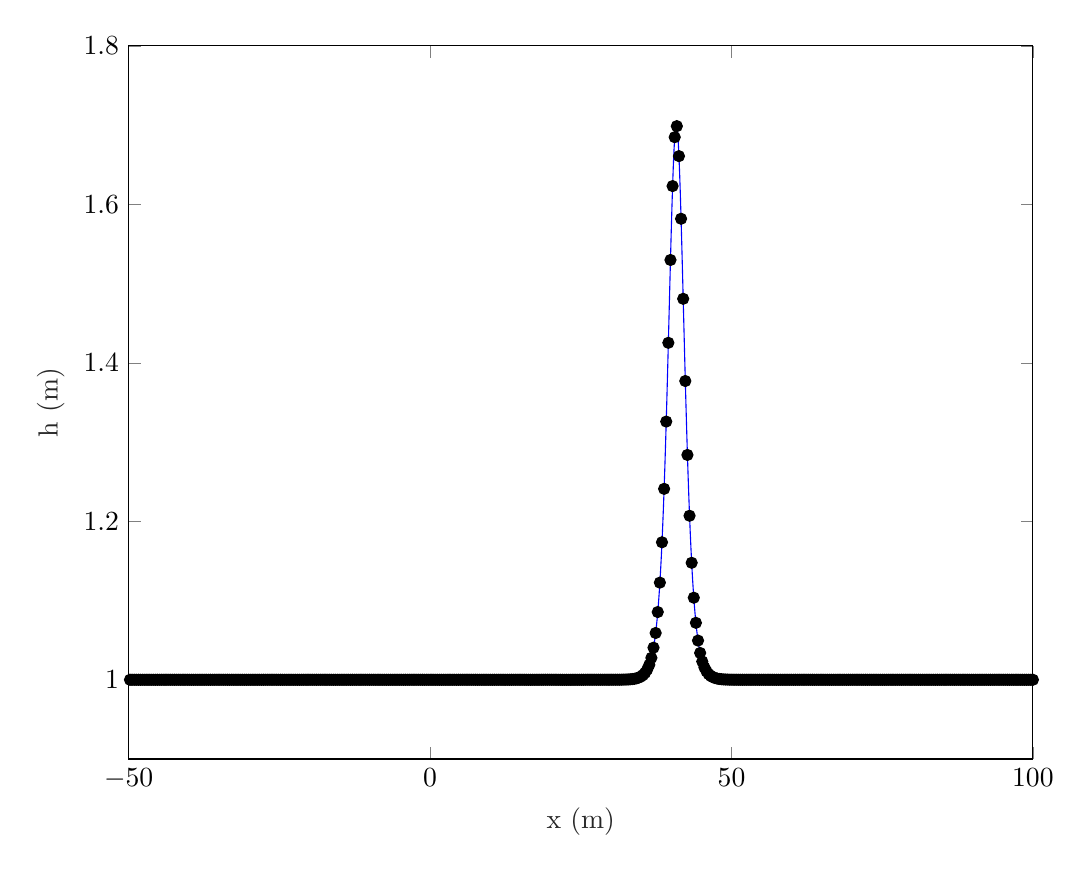
\begin{tikzpicture}

\begin{axis}[%
width=4.521in,
height=3.566in,
at={(0.758in,0.481in)},
scale only axis,
xmin=-50,
xmax=100,
xtick={-50,   0,  50, 100},
xlabel style={font=\color{white!15!black}},
xlabel={x (m)},
ymin=0.9,
ymax=1.8,
ytick={  1, 1.2, 1.4, 1.6, 1.8},
ylabel style={font=\color{white!15!black}},
ylabel={h (m)},
axis background/.style={fill=white}
]
\addplot [color=blue, forget plot]
  table[row sep=crcr]{%
-50.14064697609	1\\
-50.0234411626817	1\\
-49.9062353492733	1\\
-49.789029535865	1\\
-49.6718237224566	1\\
-49.5546179090483	1\\
-49.4374120956399	1\\
-49.3202062822316	1\\
-49.2030004688233	1\\
-49.0857946554149	1\\
-48.9685888420066	1\\
-48.8513830285982	1\\
-48.7341772151899	1\\
-48.6169714017815	1\\
-48.4997655883732	1\\
-48.3825597749648	1\\
-48.2653539615565	1\\
-48.1481481481481	1\\
-48.0309423347398	1\\
-47.9137365213315	1\\
-47.7965307079231	1\\
-47.6793248945148	1\\
-47.5621190811064	1\\
-47.4449132676981	1\\
-47.3277074542897	1\\
-47.2105016408814	1\\
-47.093295827473	1\\
-46.9760900140647	1\\
-46.8588842006564	1\\
-46.741678387248	1\\
-46.6244725738397	1\\
-46.5072667604313	1\\
-46.390060947023	1\\
-46.2728551336146	1\\
-46.1556493202063	1\\
-46.0384435067979	1\\
-45.9212376933896	1\\
-45.8040318799812	1\\
-45.6868260665729	1\\
-45.5696202531646	1\\
-45.4524144397562	1\\
-45.3352086263479	1\\
-45.2180028129395	1\\
-45.1007969995312	1\\
-44.9835911861228	1\\
-44.8663853727145	1\\
-44.7491795593061	1\\
-44.6319737458978	1\\
-44.5147679324894	1\\
-44.3975621190811	1\\
-44.2803563056728	1\\
-44.1631504922644	1\\
-44.0459446788561	1\\
-43.9287388654477	1\\
-43.8115330520394	1\\
-43.694327238631	1\\
-43.5771214252227	1\\
-43.4599156118143	1\\
-43.342709798406	1\\
-43.2255039849977	1\\
-43.1082981715893	1\\
-42.991092358181	1\\
-42.8738865447726	1\\
-42.7566807313643	1\\
-42.6394749179559	1\\
-42.5222691045476	1\\
-42.4050632911392	1\\
-42.2878574777309	1\\
-42.1706516643225	1\\
-42.0534458509142	1\\
-41.9362400375059	1\\
-41.8190342240975	1\\
-41.7018284106892	1\\
-41.5846225972808	1\\
-41.4674167838725	1\\
-41.3502109704641	1\\
-41.2330051570558	1\\
-41.1157993436474	1\\
-40.9985935302391	1\\
-40.8813877168308	1\\
-40.7641819034224	1\\
-40.6469760900141	1\\
-40.5297702766057	1\\
-40.4125644631974	1\\
-40.295358649789	1\\
-40.1781528363807	1\\
-40.0609470229723	1\\
-39.943741209564	1\\
-39.8265353961556	1\\
-39.7093295827473	1\\
-39.592123769339	1\\
-39.4749179559306	1\\
-39.3577121425223	1\\
-39.2405063291139	1\\
-39.1233005157056	1\\
-39.0060947022972	1\\
-38.8888888888889	1\\
-38.7716830754805	1\\
-38.6544772620722	1\\
-38.5372714486639	1\\
-38.4200656352555	1\\
-38.3028598218472	1\\
-38.1856540084388	1\\
-38.0684481950305	1\\
-37.9512423816221	1\\
-37.8340365682138	1\\
-37.7168307548054	1\\
-37.5996249413971	1\\
-37.4824191279887	1\\
-37.3652133145804	1\\
-37.2480075011721	1\\
-37.1308016877637	1\\
-37.0135958743554	1\\
-36.896390060947	1\\
-36.7791842475387	1\\
-36.6619784341303	1\\
-36.544772620722	1\\
-36.4275668073136	1\\
-36.3103609939053	1\\
-36.193155180497	1\\
-36.0759493670886	1\\
-35.9587435536803	1\\
-35.8415377402719	1\\
-35.7243319268636	1\\
-35.6071261134552	1\\
-35.4899203000469	1\\
-35.3727144866385	1\\
-35.2555086732302	1\\
-35.1383028598218	1\\
-35.0210970464135	1\\
-34.9038912330052	1\\
-34.7866854195968	1\\
-34.6694796061885	1\\
-34.5522737927801	1\\
-34.4350679793718	1\\
-34.3178621659634	1\\
-34.2006563525551	1\\
-34.0834505391467	1\\
-33.9662447257384	1\\
-33.8490389123301	1\\
-33.7318330989217	1\\
-33.6146272855134	1\\
-33.497421472105	1\\
-33.3802156586967	1\\
-33.2630098452883	1\\
-33.14580403188	1\\
-33.0285982184716	1\\
-32.9113924050633	1\\
-32.7941865916549	1\\
-32.6769807782466	1\\
-32.5597749648383	1\\
-32.4425691514299	1\\
-32.3253633380216	1\\
-32.2081575246132	1\\
-32.0909517112049	1\\
-31.9737458977965	1\\
-31.8565400843882	1\\
-31.7393342709798	1\\
-31.6221284575715	1\\
-31.5049226441632	1\\
-31.3877168307548	1\\
-31.2705110173465	1\\
-31.1533052039381	1\\
-31.0360993905298	1\\
-30.9188935771214	1\\
-30.8016877637131	1\\
-30.6844819503047	1\\
-30.5672761368964	1\\
-30.450070323488	1\\
-30.3328645100797	1\\
-30.2156586966714	1\\
-30.098452883263	1\\
-29.9812470698547	1\\
-29.8640412564463	1\\
-29.746835443038	1\\
-29.6296296296296	1\\
-29.5124238162213	1\\
-29.3952180028129	1\\
-29.2780121894046	1\\
-29.1608063759962	1\\
-29.0436005625879	1\\
-28.9263947491796	1\\
-28.8091889357712	1\\
-28.6919831223629	1\\
-28.5747773089545	1\\
-28.4575714955462	1\\
-28.3403656821378	1\\
-28.2231598687295	1\\
-28.1059540553211	1\\
-27.9887482419128	1\\
-27.8715424285045	1\\
-27.7543366150961	1\\
-27.6371308016878	1\\
-27.5199249882794	1\\
-27.4027191748711	1\\
-27.2855133614627	1\\
-27.1683075480544	1\\
-27.051101734646	1\\
-26.9338959212377	1\\
-26.8166901078293	1\\
-26.699484294421	1\\
-26.5822784810127	1\\
-26.4650726676043	1\\
-26.347866854196	1\\
-26.2306610407876	1\\
-26.1134552273793	1\\
-25.9962494139709	1\\
-25.8790436005626	1\\
-25.7618377871542	1\\
-25.6446319737459	1\\
-25.5274261603376	1\\
-25.4102203469292	1\\
-25.2930145335209	1\\
-25.1758087201125	1\\
-25.0586029067042	1\\
-24.9413970932958	1\\
-24.8241912798875	1\\
-24.7069854664791	1\\
-24.5897796530708	1\\
-24.4725738396624	1\\
-24.3553680262541	1\\
-24.2381622128458	1\\
-24.1209563994374	1\\
-24.0037505860291	1\\
-23.8865447726207	1\\
-23.7693389592124	1\\
-23.652133145804	1\\
-23.5349273323957	1\\
-23.4177215189873	1\\
-23.300515705579	1\\
-23.1833098921707	1\\
-23.0661040787623	1\\
-22.948898265354	1\\
-22.8316924519456	1\\
-22.7144866385373	1\\
-22.5972808251289	1\\
-22.4800750117206	1\\
-22.3628691983122	1\\
-22.2456633849039	1\\
-22.1284575714955	1\\
-22.0112517580872	1\\
-21.8940459446789	1\\
-21.7768401312705	1\\
-21.6596343178622	1\\
-21.5424285044538	1\\
-21.4252226910455	1\\
-21.3080168776371	1\\
-21.1908110642288	1\\
-21.0736052508204	1\\
-20.9563994374121	1\\
-20.8391936240038	1\\
-20.7219878105954	1\\
-20.6047819971871	1\\
-20.4875761837787	1\\
-20.3703703703704	1\\
-20.253164556962	1\\
-20.1359587435537	1\\
-20.0187529301453	1\\
-19.901547116737	1\\
-19.7843413033286	1\\
-19.6671354899203	1\\
-19.549929676512	1\\
-19.4327238631036	1\\
-19.3155180496953	1\\
-19.1983122362869	1\\
-19.0811064228786	1\\
-18.9639006094702	1\\
-18.8466947960619	1\\
-18.7294889826535	1\\
-18.6122831692452	1\\
-18.4950773558368	1\\
-18.3778715424285	1\\
-18.2606657290202	1\\
-18.1434599156118	1\\
-18.0262541022035	1\\
-17.9090482887951	1\\
-17.7918424753868	1\\
-17.6746366619784	1\\
-17.5574308485701	1\\
-17.4402250351617	1\\
-17.3230192217534	1\\
-17.2058134083451	1\\
-17.0886075949367	1\\
-16.9714017815284	1\\
-16.85419596812	1\\
-16.7369901547117	1\\
-16.6197843413033	1\\
-16.502578527895	1\\
-16.3853727144866	1\\
-16.2681669010783	1\\
-16.1509610876699	1\\
-16.0337552742616	1\\
-15.9165494608533	1\\
-15.7993436474449	1\\
-15.6821378340366	1\\
-15.5649320206282	1\\
-15.4477262072199	1\\
-15.3305203938115	1\\
-15.2133145804032	1\\
-15.0961087669948	1\\
-14.9789029535865	1\\
-14.8616971401782	1\\
-14.7444913267698	1\\
-14.6272855133615	1\\
-14.5100796999531	1\\
-14.3928738865448	1\\
-14.2756680731364	1\\
-14.1584622597281	1\\
-14.0412564463197	1\\
-13.9240506329114	1\\
-13.806844819503	1\\
-13.6896390060947	1\\
-13.5724331926864	1\\
-13.455227379278	1\\
-13.3380215658697	1\\
-13.2208157524613	1\\
-13.103609939053	1\\
-12.9864041256446	1\\
-12.8691983122363	1\\
-12.7519924988279	1\\
-12.6347866854196	1\\
-12.5175808720113	1\\
-12.4003750586029	1\\
-12.2831692451946	1\\
-12.1659634317862	1\\
-12.0487576183779	1\\
-11.9315518049695	1\\
-11.8143459915612	1\\
-11.6971401781528	1\\
-11.5799343647445	1\\
-11.4627285513361	1\\
-11.3455227379278	1\\
-11.2283169245195	1\\
-11.1111111111111	1\\
-10.9939052977028	1\\
-10.8766994842944	1\\
-10.7594936708861	1\\
-10.6422878574777	1\\
-10.5250820440694	1\\
-10.407876230661	1\\
-10.2906704172527	1\\
-10.1734646038444	1\\
-10.056258790436	1\\
-9.93905297702766	1\\
-9.82184716361932	1\\
-9.70464135021097	1\\
-9.58743553680262	1\\
-9.47022972339428	1\\
-9.35302390998594	1\\
-9.23581809657759	1\\
-9.11861228316924	1\\
-9.0014064697609	1\\
-8.88420065635255	1\\
-8.76699484294421	1\\
-8.64978902953587	1\\
-8.53258321612752	1\\
-8.41537740271917	1\\
-8.29817158931083	1\\
-8.18096577590249	1\\
-8.06375996249414	1\\
-7.94655414908579	1\\
-7.82934833567745	1\\
-7.7121425222691	1\\
-7.59493670886076	1\\
-7.47773089545242	1\\
-7.36052508204407	1\\
-7.24331926863572	1\\
-7.12611345522738	1\\
-7.00890764181904	1\\
-6.89170182841069	1\\
-6.77449601500234	1\\
-6.657290201594	1\\
-6.54008438818565	1\\
-6.42287857477731	1\\
-6.30567276136896	1\\
-6.18846694796062	1\\
-6.07126113455227	1\\
-5.95405532114393	1\\
-5.83684950773559	1\\
-5.71964369432724	1\\
-5.60243788091889	1\\
-5.48523206751055	1\\
-5.3680262541022	1\\
-5.25082044069386	1\\
-5.13361462728551	1\\
-5.01640881387717	1\\
-4.89920300046882	1\\
-4.78199718706048	1\\
-4.66479137365214	1\\
-4.54758556024379	1\\
-4.43037974683544	1\\
-4.31317393342709	1\\
-4.19596812001875	1\\
-4.07876230661041	1\\
-3.96155649320206	1\\
-3.84435067979372	1\\
-3.72714486638537	1\\
-3.60993905297703	1\\
-3.49273323956868	1\\
-3.37552742616034	1\\
-3.25832161275199	1\\
-3.14111579934364	1\\
-3.0239099859353	1\\
-2.90670417252696	1\\
-2.78949835911861	1\\
-2.67229254571027	1\\
-2.55508673230192	1\\
-2.43788091889358	1\\
-2.32067510548523	1\\
-2.20346929207689	1\\
-2.08626347866854	1\\
-1.96905766526019	1\\
-1.85185185185185	1\\
-1.73464603844351	1\\
-1.61744022503516	1\\
-1.50023441162681	1\\
-1.38302859821847	1\\
-1.26582278481013	1\\
-1.14861697140178	1\\
-1.03141115799344	1\\
-0.914205344585092	1\\
-0.796999531176745	1\\
-0.679793717768398	1\\
-0.562587904360058	1\\
-0.445382090951711	1\\
-0.328176277543363	1\\
-0.210970464135023	1\\
-0.0937646507266763	1\\
0.0234411626816708	1\\
0.140646976090011	1\\
0.257852789498358	1\\
0.375058602906705	1\\
0.492264416315052	1\\
0.609470229723392	1\\
0.726676043131739	1\\
0.843881856540087	1\\
0.961087669948427	1\\
1.07829348335677	1\\
1.19549929676512	1\\
1.31270511017347	1\\
1.42991092358181	1\\
1.54711673699016	1\\
1.6643225503985	1\\
1.78152836380684	1\\
1.89873417721519	1\\
2.01593999062354	1\\
2.13314580403188	1\\
2.25035161744022	1\\
2.36755743084857	1\\
2.48476324425692	1\\
2.60196905766526	1\\
2.71917487107361	1\\
2.83638068448195	1\\
2.95358649789029	1\\
3.07079231129864	1\\
3.18799812470699	1\\
3.30520393811533	1\\
3.42240975152367	1\\
3.53961556493202	1\\
3.65682137834037	1\\
3.77402719174871	1\\
3.89123300515705	1\\
4.0084388185654	1\\
4.12564463197375	1\\
4.24285044538209	1\\
4.36005625879044	1\\
4.47726207219878	1\\
4.59446788560712	1\\
4.71167369901547	1\\
4.82887951242382	1\\
4.94608532583216	1\\
5.0632911392405	1\\
5.18049695264885	1\\
5.2977027660572	1\\
5.41490857946554	1\\
5.53211439287389	1\\
5.64932020628223	1\\
5.76652601969058	1\\
5.88373183309892	1\\
6.00093764650727	1\\
6.11814345991561	1\\
6.23534927332395	1\\
6.3525550867323	1\\
6.46976090014065	1\\
6.58696671354899	1\\
6.70417252695734	1\\
6.82137834036568	1\\
6.93858415377403	1\\
7.05578996718237	1\\
7.17299578059072	1\\
7.29020159399906	1\\
7.4074074074074	1\\
7.52461322081575	1\\
7.6418190342241	1\\
7.75902484763245	1\\
7.87623066104079	1\\
7.99343647444913	1\\
8.11064228785748	1\\
8.22784810126582	1\\
8.34505391467417	1\\
8.46225972808251	1\\
8.57946554149086	1\\
8.6966713548992	1\\
8.81387716830755	1\\
8.9310829817159	1\\
9.04828879512424	1\\
9.16549460853258	1\\
9.28270042194093	1\\
9.39990623534927	1\\
9.51711204875762	1\\
9.63431786216596	1\\
9.75152367557431	1\\
9.86872948898265	1\\
9.985935302391	1\\
10.1031411157993	1\\
10.2203469292077	1\\
10.337552742616	1.00000000000001\\
10.4547585560244	1.00000000000001\\
10.5719643694327	1.00000000000001\\
10.6891701828411	1.00000000000001\\
10.8063759962494	1.00000000000001\\
10.9235818096578	1.00000000000001\\
11.0407876230661	1.00000000000001\\
11.1579934364744	1.00000000000001\\
11.2751992498828	1.00000000000001\\
11.3924050632911	1.00000000000002\\
11.5096108766995	1.00000000000002\\
11.6268166901078	1.00000000000002\\
11.7440225035162	1.00000000000003\\
11.8612283169245	1.00000000000003\\
11.9784341303329	1.00000000000003\\
12.0956399437412	1.00000000000004\\
12.2128457571496	1.00000000000004\\
12.3300515705579	1.00000000000005\\
12.4472573839662	1.00000000000005\\
12.5644631973746	1.00000000000006\\
12.6816690107829	1.00000000000007\\
12.7988748241913	1.00000000000008\\
12.9160806375996	1.00000000000009\\
13.033286451008	1.00000000000011\\
13.1504922644163	1.00000000000012\\
13.2676980778247	1.00000000000014\\
13.384903891233	1.00000000000016\\
13.5021097046413	1.00000000000018\\
13.6193155180497	1.0000000000002\\
13.736521331458	1.00000000000023\\
13.8537271448664	1.00000000000026\\
13.9709329582747	1.0000000000003\\
14.0881387716831	1.00000000000034\\
14.2053445850914	1.00000000000039\\
14.3225503984998	1.00000000000044\\
14.4397562119081	1.0000000000005\\
14.5569620253165	1.00000000000057\\
14.6741678387248	1.00000000000065\\
14.7913736521331	1.00000000000074\\
14.9085794655415	1.00000000000085\\
15.0257852789498	1.00000000000096\\
15.1429910923582	1.0000000000011\\
15.2601969057665	1.00000000000125\\
15.3774027191749	1.00000000000142\\
15.4946085325832	1.00000000000162\\
15.6118143459916	1.00000000000185\\
15.7290201593999	1.00000000000211\\
15.8462259728083	1.0000000000024\\
15.9634317862166	1.00000000000273\\
16.0806375996249	1.00000000000311\\
16.1978434130333	1.00000000000354\\
16.3150492264416	1.00000000000404\\
16.43225503985	1.0000000000046\\
16.5494608532583	1.00000000000524\\
16.6666666666667	1.00000000000597\\
16.783872480075	1.0000000000068\\
16.9010782934834	1.00000000000775\\
17.0182841068917	1.00000000000882\\
17.1354899203	1.00000000001005\\
17.2526957337084	1.00000000001145\\
17.3699015471167	1.00000000001304\\
17.4871073605251	1.00000000001486\\
17.6043131739334	1.00000000001692\\
17.7215189873418	1.00000000001928\\
17.8387248007501	1.00000000002196\\
17.9559306141585	1.00000000002502\\
18.0731364275668	1.0000000000285\\
18.1903422409752	1.00000000003246\\
18.3075480543835	1.00000000003698\\
18.4247538677918	1.00000000004212\\
18.5419596812002	1.00000000004798\\
18.6591654946085	1.00000000005466\\
18.7763713080169	1.00000000006226\\
18.8935771214252	1.00000000007093\\
19.0107829348336	1.00000000008079\\
19.1279887482419	1.00000000009204\\
19.2451945616503	1.00000000010484\\
19.3624003750586	1.00000000011943\\
19.4796061884669	1.00000000013604\\
19.5968120018753	1.00000000015497\\
19.7140178152836	1.00000000017653\\
19.831223628692	1.00000000020109\\
19.9484294421003	1.00000000022907\\
20.0656352555087	1.00000000026094\\
20.182841068917	1.00000000029725\\
20.3000468823254	1.00000000033861\\
20.4172526957337	1.00000000038572\\
20.5344585091421	1.00000000043938\\
20.6516643225504	1.00000000050052\\
20.7688701359587	1.00000000057015\\
20.8860759493671	1.00000000064948\\
21.0032817627754	1.00000000073985\\
21.1204875761838	1.00000000084278\\
21.2376933895921	1.00000000096004\\
21.3548992030005	1.00000000109361\\
21.4721050164088	1.00000000124577\\
21.5893108298172	1.0000000014191\\
21.7065166432255	1.00000000161654\\
21.8237224566338	1.00000000184145\\
21.9409282700422	1.00000000209766\\
22.0581340834505	1.00000000238951\\
22.1753398968589	1.00000000272197\\
22.2925457102672	1.00000000310068\\
22.4097515236756	1.00000000353209\\
22.5269573370839	1.00000000402352\\
22.6441631504923	1.00000000458332\\
22.7613689639006	1.00000000522101\\
22.878574777309	1.00000000594742\\
22.9957805907173	1.0000000067749\\
23.1129864041256	1.00000000771751\\
23.230192217534	1.00000000879126\\
23.3473980309423	1.00000001001441\\
23.4646038443507	1.00000001140774\\
23.581809657759	1.00000001299493\\
23.6990154711674	1.00000001480295\\
23.8162212845757	1.00000001686252\\
23.9334270979841	1.00000001920864\\
24.0506329113924	1.00000002188119\\
24.1678387248007	1.00000002492557\\
24.2850445382091	1.00000002839353\\
24.4022503516174	1.00000003234399\\
24.5194561650258	1.00000003684409\\
24.6366619784341	1.00000004197029\\
24.7538677918425	1.00000004780973\\
24.8710736052508	1.00000005446161\\
24.9882794186592	1.00000006203899\\
25.1054852320675	1.00000007067062\\
25.2226910454759	1.0000000805032\\
25.3398968588842	1.00000009170381\\
25.4571026722925	1.00000010446279\\
25.5743084857009	1.00000011899695\\
25.6915142991092	1.00000013555329\\
25.8087201125176	1.00000015441315\\
25.9259259259259	1.00000017589703\\
26.0431317393343	1.00000020037001\\
26.1603375527426	1.00000022824798\\
26.277543366151	1.00000026000468\\
26.3947491795593	1.00000029617977\\
26.5119549929676	1.00000033738798\\
26.629160806376	1.00000038432959\\
26.7463666197843	1.0000004378023\\
26.8635724331927	1.00000049871479\\
26.980778246601	1.00000056810218\\
27.0979840600094	1.0000006471436\\
27.2151898734177	1.00000073718224\\
27.3323956868261	1.00000083974816\\
27.4496015002344	1.00000095658431\\
27.5668073136428	1.00000108967614\\
27.6840131270511	1.00000124128534\\
27.8012189404594	1.00000141398825\\
27.9184247538678	1.0000016107197\\
28.0356305672761	1.00000183482281\\
28.1528363806845	1.00000209010585\\
28.2700421940928	1.00000238090694\\
28.3872480075012	1.00000271216775\\
28.5044538209095	1.00000308951751\\
28.6216596343179	1.00000351936862\\
28.7388654477262	1.00000400902566\\
28.8560712611346	1.00000456680947\\
28.9732770745429	1.00000520219857\\
29.0904828879512	1.00000592599023\\
29.2076887013596	1.00000675048389\\
29.3248945147679	1.0000076896902\\
29.4421003281763	1.00000875956908\\
29.5593061415846	1.00000997830084\\
29.676511954993	1.00001136659518\\
29.7937177684013	1.00001294804298\\
29.9109235818097	1.00001474951715\\
30.028129395218	1.00001680162923\\
30.1453352086263	1.00001913924939\\
30.2625410220347	1.00002180209889\\
30.379746835443	1.00002483542488\\
30.4969526488514	1.00002829076897\\
30.6141584622597	1.00003222684283\\
30.7313642756681	1.00003671052539\\
30.8485700890764	1.00004181799877\\
30.9657759024848	1.00004763604212\\
31.0829817158931	1.00005426350526\\
31.2001875293015	1.00006181298725\\
31.3173933427098	1.00007041274808\\
31.4345991561181	1.00008020888611\\
31.5518049695265	1.00009136781794\\
31.6690107829348	1.00010407910273\\
31.7862165963432	1.00011855865867\\
31.9034224097515	1.00013505242597\\
32.0206282231599	1.00015384053823\\
32.1378340365682	1.00017524207239\\
32.2550398499766	1.00019962045743\\
32.3722456633849	1.00022738963267\\
32.4894514767932	1.00025902105926\\
32.6066572902016	1.00029505170228\\
32.7238631036099	1.00033609311725\\
32.8410689170183	1.0003828417927\\
32.9582747304266	1.00043609092128\\
33.075480543835	1.00049674379492\\
33.1926863572433	1.00056582904603\\
33.3098921706517	1.00064451798632\\
33.42709798406	1.00073414432823\\
33.5443037974684	1.00083622661165\\
33.6615096108767	1.00095249370097\\
33.778715424285	1.0010849137646\\
33.8959212376934	1.00123572720247\\
34.0131270511017	1.00140748404565\\
34.1303328645101	1.00160308641825\\
34.2475386779184	1.00182583672379\\
34.3647444913268	1.00207949229868\\
34.4819503047351	1.00236832736205\\
34.5991561181435	1.00269720318669\\
34.7163619315518	1.00307164751712\\
34.8335677449601	1.00349794436982\\
34.9507735583685	1.00398323546349\\
35.0679793717768	1.00453563464401\\
35.1851851851852	1.00516435678464\\
35.3023909985935	1.00587986275291\\
35.4195968120019	1.00669402213515\\
35.5368026254102	1.00762029548797\\
35.6540084388186	1.00867393793132\\
35.7712142522269	1.00987222589332\\
35.8884200656353	1.0112347087405\\
36.0056258790436	1.01278348685073\\
36.122831692452	1.01454351737156\\
36.2400375058603	1.01654294840809\\
36.3572433192686	1.01881348163989\\
36.474449132677	1.02139076230266\\
36.5916549460853	1.02431479399257\\
36.7088607594937	1.02763037374657\\
36.826066572902	1.03138754018544\\
36.9432723863104	1.03564202401603\\
37.0604781997187	1.04045568569542\\
37.177684013127	1.04589691935839\\
37.2948898265354	1.05204099499315\\
37.4120956399437	1.05897030211297\\
37.5293014533521	1.06677444764938\\
37.6465072667604	1.07555014839734\\
37.7637130801688	1.08540084413538\\
37.8809188935771	1.09643594181754\\
37.9981247069855	1.10876958464425\\
38.1153305203938	1.12251882353235\\
38.2325363338022	1.13780105438818\\
38.3497421472105	1.15473057541087\\
38.4669479606189	1.17341411827757\\
38.5841537740272	1.1939452205691\\
38.7013595874355	1.21639734045667\\
38.8185654008439	1.24081567565857\\
38.9357712142522	1.26720774434257\\
39.0529770276606	1.2955329222128\\
39.1701828410689	1.32569131053987\\
39.2873886544773	1.35751253148912\\
39.4045944678856	1.390745297658\\
39.5218002812939	1.42504885763197\\
39.6390060947023	1.45998763933329\\
39.7562119081106	1.49503054446875\\
39.873417721519	1.52955632751224\\
39.9906235349273	1.56286625940054\\
40.1078293483357	1.59420478473859\\
40.225035161744	1.62278812430555\\
40.3422409751524	1.64783980054667\\
40.4594467885607	1.66863098727213\\
40.5766526019691	1.68452258078498\\
40.6938584153774	1.69500516570792\\
40.8110642287858	1.69973279861715\\
40.9282700421941	1.69854688081361\\
41.0454758556024	1.69148734707972\\
41.1626816690108	1.67878983410198\\
41.2798874824191	1.66086916888311\\
41.3970932958275	1.63829113257875\\
41.5142991092358	1.61173572291671\\
41.6315049226442	1.58195585851466\\
41.7487107360525	1.54973556893153\\
41.8659165494608	1.51585125455816\\
41.9831223628692	1.48103873924162\\
42.1003281762775	1.44596778161234\\
42.2175339896859	1.41122465757309\\
42.3347398030942	1.3773025291539\\
42.4519456165026	1.34459866185464\\
42.5691514299109	1.3134171679134\\
42.6863572433193	1.28397581179477\\
42.8035630567276	1.25641546268183\\
42.920768870136	1.23081095285464\\
43.0379746835443	1.20718234045221\\
43.1551804969527	1.18550583214261\\
43.272386310361	1.16572386238546\\
43.3895921237693	1.14775403199658\\
43.5067979371777	1.13149677160441\\
43.624003750586	1.11684171519414\\
43.7412095639944	1.10367284988357\\
43.8584153774027	1.09187255723844\\
43.9756211908111	1.08132468621399\\
44.0928270042194	1.07191680507409\\
44.2100328176277	1.06354177520369\\
44.3272386310361	1.05609877817921\\
44.4444444444444	1.04949391219976\\
44.5616502578528	1.04364045739367\\
44.6788560712611	1.03845889316303\\
44.7960618846695	1.033876735555\\
44.9132676980778	1.02982824914637\\
45.0304735114862	1.02625407628462\\
45.1476793248945	1.02310081673667\\
45.2648851383029	1.02032058273039\\
45.3820909517112	1.01787054784875\\
45.4992967651196	1.01571250304345\\
45.6165025785279	1.01381242896519\\
45.7337083919362	1.01214009066847\\
45.8509142053446	1.01066865836391\\
45.9681200187529	1.00937435611301\\
46.0853258321613	1.00823613906005\\
46.2025316455696	1.00723539886986\\
46.319737458978	1.00635569640231\\
46.4369432723863	1.0055825202356\\
46.5541490857947	1.0049030693964\\
46.671354899203	1.00430605852224\\
46.7885607126113	1.00378154363688\\
46.9057665260197	1.00332076673743\\
47.022972339428	1.0029160174518\\
47.1401781528364	1.00256051011353\\
47.2573839662447	1.00224827470599\\
47.3745897796531	1.00197406024124\\
47.4917955930614	1.00173324925606\\
47.6090014064698	1.00152178222268\\
47.7262072198781	1.00133609078359\\
47.8434130332865	1.00117303882565\\
47.9606188466948	1.00102987050806\\
48.0778246601031	1.00090416445011\\
48.1950304735115	1.00079379336951\\
48.3122362869198	1.0006968885386\\
48.4294421003282	1.00061180849548\\
48.5466479137365	1.00053711151023\\
48.6638537271449	1.00047153136275\\
48.7810595405532	1.00041395603937\\
48.8982653539616	1.00036340900106\\
49.0154711673699	1.00031903271587\\
49.1326769807782	1.0002800741846\\
49.2498827941866	1.00024587222034\\
49.3670886075949	1.00021584627088\\
49.4842944210033	1.00018948659805\\
49.6015002344116	1.00016634565013\\
49.71870604782	1.00014603048306\\
49.8359118612283	1.00012819610352\\
49.9531176746367	1.00011253962214\\
50.070323488045	1.00009879511859\\
50.1875293014534	1.00008672913208\\
50.3047351148617	1.00007613670128\\
50.42194092827	1.00006683788695\\
50.5391467416784	1.0000586747184\\
50.6563525550867	1.00005150851238\\
50.7735583684951	1.00004521751891\\
50.8907641819034	1.0000396948543\\
51.0079699953118	1.00003484668635\\
51.1251758087201	1.00003059064095\\
51.2423816221285	1.00002685440323\\
51.3595874355368	1.0000235744893\\
51.4767932489451	1.00002069516802\\
51.5939990623535	1.00001816751431\\
51.7112048757618	1.00001594857809\\
51.8284106891702	1.00001400065467\\
51.9456165025785	1.00001229064413\\
52.0628223159869	1.00001078948908\\
52.1800281293952	1.00000947168091\\
52.2972339428036	1.00000831482643\\
52.4144397562119	1.00000729926738\\
52.5316455696203	1.00000640774646\\
52.6488513830286	1.00000562511405\\
52.7660571964369	1.00000493807084\\
52.8832630098453	1.00000433494182\\
53.0004688232536	1.00000380547792\\
53.117674636662	1.00000334068188\\
53.2348804500703	1.00000293265529\\
53.3520862634787	1.00000257446445\\
53.469292076887	1.00000226002252\\
53.5864978902954	1.00000198398609\\
53.7037037037037	1.00000174166437\\
53.820909517112	1.00000152893951\\
53.9381153305204	1.00000134219659\\
54.0553211439287	1.00000117826222\\
54.1725269573371	1.00000103435059\\
54.2897327707454	1.00000090801616\\
54.4069385841538	1.00000079711206\\
54.5241443975621	1.00000069975366\\
54.6413502109705	1.00000061428651\\
54.7585560243788	1.00000053925822\\
54.8757618377872	1.0000004733938\\
54.9929676511955	1.00000041557398\\
55.1101734646038	1.00000036481622\\
55.2273792780122	1.00000032025795\\
55.3445850914205	1.00000028114198\\
55.4617909048289	1.0000002468036\\
55.5789967182372	1.00000021665926\\
55.6962025316456	1.00000019019673\\
55.8134083450539	1.0000001669663\\
55.9306141584623	1.00000014657321\\
56.0478199718706	1.00000012867091\\
56.165025785279	1.00000011295518\\
56.2822315986873	1.00000009915895\\
56.3994374120956	1.00000008704778\\
56.516643225504	1.00000007641585\\
56.6338490389123	1.0000000670825\\
56.7510548523207	1.00000005888911\\
56.868260665729	1.00000005169646\\
56.9854664791374	1.00000004538231\\
57.1026722925457	1.00000003983936\\
57.2198781059541	1.00000003497342\\
57.3370839193624	1.0000000307018\\
57.4542897327707	1.00000002695192\\
57.5714955461791	1.00000002366004\\
57.6887013595874	1.00000002077022\\
57.8059071729958	1.00000001823337\\
57.9231129864041	1.00000001600637\\
58.0403187998125	1.00000001405136\\
58.1575246132208	1.00000001233515\\
58.2747304266292	1.00000001082854\\
58.3919362400375	1.00000000950596\\
58.5091420534459	1.00000000834491\\
58.6263478668542	1.00000000732567\\
58.7435536802625	1.00000000643092\\
58.8607594936709	1.00000000564545\\
58.9779653070792	1.00000000495592\\
59.0951711204876	1.00000000435061\\
59.2123769338959	1.00000000381923\\
59.3295827473043	1.00000000335276\\
59.4467885607126	1.00000000294325\\
59.563994374121	1.00000000258377\\
59.6812001875293	1.00000000226819\\
59.7984060009376	1.00000000199116\\
59.915611814346	1.00000000174796\\
60.0328176277543	1.00000000153446\\
60.1500234411627	1.00000000134705\\
60.267229254571	1.00000000118252\\
60.3844350679794	1.00000000103809\\
60.5016408813877	1.0000000009113\\
60.6188466947961	1.00000000079999\\
60.7360525082044	1.00000000070228\\
60.8532583216128	1.00000000061651\\
60.9704641350211	1.00000000054121\\
61.0876699484294	1.0000000004751\\
61.2048757618378	1.00000000041708\\
61.3220815752461	1.00000000036613\\
61.4392873886545	1.00000000032141\\
61.5564932020628	1.00000000028216\\
61.6736990154712	1.00000000024769\\
61.7909048288795	1.00000000021744\\
61.9081106422879	1.00000000019088\\
62.0253164556962	1.00000000016757\\
62.1425222691045	1.0000000001471\\
62.2597280825129	1.00000000012914\\
62.3769338959212	1.00000000011336\\
62.4941397093296	1.00000000009952\\
62.6113455227379	1.00000000008736\\
62.7285513361463	1.00000000007669\\
62.8457571495546	1.00000000006732\\
62.962962962963	1.0000000000591\\
63.0801687763713	1.00000000005188\\
63.1973745897797	1.00000000004555\\
63.314580403188	1.00000000003998\\
63.4317862165964	1.0000000000351\\
63.5489920300047	1.00000000003081\\
63.666197843413	1.00000000002705\\
63.7834036568214	1.00000000002375\\
63.9006094702297	1.00000000002085\\
64.0178152836381	1.0000000000183\\
64.1350210970464	1.00000000001606\\
64.2522269104548	1.0000000000141\\
64.3694327238631	1.00000000001238\\
64.4866385372714	1.00000000001087\\
64.6038443506798	1.00000000000954\\
64.7210501640881	1.00000000000838\\
64.8382559774965	1.00000000000735\\
64.9554617909048	1.00000000000645\\
65.0726676043132	1.00000000000567\\
65.1898734177215	1.00000000000497\\
65.3070792311299	1.00000000000437\\
65.4242850445382	1.00000000000383\\
65.5414908579466	1.00000000000336\\
65.6586966713549	1.00000000000295\\
65.7759024847633	1.00000000000259\\
65.8931082981716	1.00000000000228\\
66.0103141115799	1.000000000002\\
66.1275199249883	1.00000000000175\\
66.2447257383966	1.00000000000154\\
66.361931551805	1.00000000000135\\
66.4791373652133	1.00000000000119\\
66.5963431786217	1.00000000000104\\
66.71354899203	1.00000000000091\\
66.8307548054383	1.0000000000008\\
66.9479606188467	1.0000000000007\\
67.065166432255	1.00000000000062\\
67.1823722456634	1.00000000000054\\
67.2995780590717	1.00000000000048\\
67.4167838724801	1.00000000000042\\
67.5339896858884	1.00000000000037\\
67.6511954992968	1.00000000000032\\
67.7684013127051	1.00000000000028\\
67.8856071261135	1.00000000000025\\
68.0028129395218	1.00000000000022\\
68.1200187529302	1.00000000000019\\
68.2372245663385	1.00000000000017\\
68.3544303797468	1.00000000000015\\
68.4716361931552	1.00000000000013\\
68.5888420065635	1.00000000000011\\
68.7060478199719	1.0000000000001\\
68.8232536333802	1.00000000000009\\
68.9404594467886	1.00000000000008\\
69.0576652601969	1.00000000000007\\
69.1748710736052	1.00000000000006\\
69.2920768870136	1.00000000000005\\
69.4092827004219	1.00000000000005\\
69.5264885138303	1.00000000000004\\
69.6436943272386	1.00000000000004\\
69.760900140647	1.00000000000003\\
69.8781059540553	1.00000000000003\\
69.9953117674637	1.00000000000002\\
70.112517580872	1.00000000000002\\
70.2297233942804	1.00000000000002\\
70.3469292076887	1.00000000000002\\
70.4641350210971	1.00000000000001\\
70.5813408345054	1.00000000000001\\
70.6985466479137	1.00000000000001\\
70.8157524613221	1.00000000000001\\
70.9329582747304	1.00000000000001\\
71.0501640881388	1.00000000000001\\
71.1673699015471	1.00000000000001\\
71.2845757149555	1.00000000000001\\
71.4017815283638	1\\
71.5189873417721	1\\
71.6361931551805	1\\
71.7533989685888	1\\
71.8706047819972	1\\
71.9878105954055	1\\
72.1050164088139	1\\
72.2222222222222	1\\
72.3394280356306	1\\
72.4566338490389	1\\
72.5738396624473	1\\
72.6910454758556	1\\
72.8082512892639	1\\
72.9254571026723	1\\
73.0426629160806	1\\
73.159868729489	1\\
73.2770745428973	1\\
73.3942803563057	1\\
73.511486169714	1\\
73.6286919831224	1\\
73.7458977965307	1\\
73.8631036099391	1\\
73.9803094233474	1\\
74.0975152367557	1\\
74.2147210501641	1\\
74.3319268635724	1\\
74.4491326769808	1\\
74.5663384903891	1\\
74.6835443037975	1\\
74.8007501172058	1\\
74.9179559306142	1\\
75.0351617440225	1\\
75.1523675574308	1\\
75.2695733708392	1\\
75.3867791842475	1\\
75.5039849976559	1\\
75.6211908110642	1\\
75.7383966244726	1\\
75.8556024378809	1\\
75.9728082512893	1\\
76.0900140646976	1\\
76.207219878106	1\\
76.3244256915143	1\\
76.4416315049226	1\\
76.558837318331	1\\
76.6760431317393	1\\
76.7932489451477	1\\
76.910454758556	1\\
77.0276605719644	1\\
77.1448663853727	1\\
77.2620721987811	1\\
77.3792780121894	1\\
77.4964838255977	1\\
77.6136896390061	1\\
77.7308954524144	1\\
77.8481012658228	1\\
77.9653070792311	1\\
78.0825128926395	1\\
78.1997187060478	1\\
78.3169245194562	1\\
78.4341303328645	1\\
78.5513361462729	1\\
78.6685419596812	1\\
78.7857477730896	1\\
78.9029535864979	1\\
79.0201593999062	1\\
79.1373652133146	1\\
79.2545710267229	1\\
79.3717768401313	1\\
79.4889826535396	1\\
79.606188466948	1\\
79.7233942803563	1\\
79.8406000937647	1\\
79.957805907173	1\\
80.0750117205813	1\\
80.1922175339897	1\\
80.309423347398	1\\
80.4266291608064	1\\
80.5438349742147	1\\
80.6610407876231	1\\
80.7782466010314	1\\
80.8954524144397	1\\
81.0126582278481	1\\
81.1298640412564	1\\
81.2470698546648	1\\
81.3642756680731	1\\
81.4814814814815	1\\
81.5986872948898	1\\
81.7158931082982	1\\
81.8330989217065	1\\
81.9503047351149	1\\
82.0675105485232	1\\
82.1847163619315	1\\
82.3019221753399	1\\
82.4191279887482	1\\
82.5363338021566	1\\
82.6535396155649	1\\
82.7707454289733	1\\
82.8879512423816	1\\
83.00515705579	1\\
83.1223628691983	1\\
83.2395686826067	1\\
83.356774496015	1\\
83.4739803094234	1\\
83.5911861228317	1\\
83.70839193624	1\\
83.8255977496484	1\\
83.9428035630567	1\\
84.0600093764651	1\\
84.1772151898734	1\\
84.2944210032818	1\\
84.4116268166901	1\\
84.5288326300985	1\\
84.6460384435068	1\\
84.7632442569152	1\\
84.8804500703235	1\\
84.9976558837318	1\\
85.1148616971402	1\\
85.2320675105485	1\\
85.3492733239569	1\\
85.4664791373652	1\\
85.5836849507735	1\\
85.7008907641819	1\\
85.8180965775902	1\\
85.9353023909986	1\\
86.0525082044069	1\\
86.1697140178153	1\\
86.2869198312236	1\\
86.404125644632	1\\
86.5213314580403	1\\
86.6385372714487	1\\
86.755743084857	1\\
86.8729488982653	1\\
86.9901547116737	1\\
87.107360525082	1\\
87.2245663384904	1\\
87.3417721518987	1\\
87.4589779653071	1\\
87.5761837787154	1\\
87.6933895921238	1\\
87.8105954055321	1\\
87.9278012189405	1\\
88.0450070323488	1\\
88.1622128457572	1\\
88.2794186591655	1\\
88.3966244725738	1\\
88.5138302859822	1\\
88.6310360993905	1\\
88.7482419127989	1\\
88.8654477262072	1\\
88.9826535396156	1\\
89.0998593530239	1\\
89.2170651664323	1\\
89.3342709798406	1\\
89.451476793249	1\\
89.5686826066573	1\\
89.6858884200656	1\\
89.803094233474	1\\
89.9203000468823	1\\
90.0375058602907	1\\
90.154711673699	1\\
90.2719174871074	1\\
90.3891233005157	1\\
90.506329113924	1\\
90.6235349273324	1\\
90.7407407407407	1\\
90.8579465541491	1\\
90.9751523675574	1\\
91.0923581809658	1\\
91.2095639943741	1\\
91.3267698077825	1\\
91.4439756211908	1\\
91.5611814345991	1\\
91.6783872480075	1\\
91.7955930614158	1\\
91.9127988748242	1\\
92.0300046882325	1\\
92.1472105016409	1\\
92.2644163150492	1\\
92.3816221284576	1\\
92.4988279418659	1\\
92.6160337552743	1\\
92.7332395686826	1\\
92.850445382091	1\\
92.9676511954993	1\\
93.0848570089076	1\\
93.202062822316	1\\
93.3192686357243	1\\
93.4364744491327	1\\
93.553680262541	1\\
93.6708860759494	1\\
93.7880918893577	1\\
93.9052977027661	1\\
94.0225035161744	1\\
94.1397093295828	1\\
94.2569151429911	1\\
94.3741209563995	1\\
94.4913267698078	1\\
94.6085325832161	1\\
94.7257383966245	1\\
94.8429442100328	1\\
94.9601500234412	1\\
95.0773558368495	1\\
95.1945616502579	1\\
95.3117674636662	1\\
95.4289732770745	1\\
95.5461790904829	1\\
95.6633849038912	1\\
95.7805907172996	1\\
95.8977965307079	1\\
96.0150023441163	1\\
96.1322081575246	1\\
96.2494139709329	1\\
96.3666197843413	1\\
96.4838255977496	1\\
96.601031411158	1\\
96.7182372245663	1\\
96.8354430379747	1\\
96.952648851383	1\\
97.0698546647914	1\\
97.1870604781997	1\\
97.3042662916081	1\\
97.4214721050164	1\\
97.5386779184248	1\\
97.6558837318331	1\\
97.7730895452414	1\\
97.8902953586498	1\\
98.0075011720581	1\\
98.1247069854665	1\\
98.2419127988748	1\\
98.3591186122832	1\\
98.4763244256915	1\\
98.5935302390999	1\\
98.7107360525082	1\\
98.8279418659166	1\\
98.9451476793249	1\\
99.0623534927333	1\\
99.1795593061416	1\\
99.2967651195499	1\\
99.4139709329583	1\\
99.5311767463666	1\\
99.648382559775	1\\
99.7655883731833	1\\
99.8827941865917	1\\
100	1\\
100.117205813408	1\\
};
\addplot [color=black, draw=none, mark=*, mark options={solid, black}, forget plot]
  table[row sep=crcr]{%
-50.14064697609	1\\
-49.789029535865	0.999999999844261\\
-49.4374120956399	0.999999999827231\\
-49.0857946554149	0.999999999796034\\
-48.7341772151899	0.999999999748626\\
-48.3825597749648	0.999999999681601\\
-48.0309423347398	0.999999999590216\\
-47.6793248945148	0.999999999468107\\
-47.3277074542897	0.999999999306914\\
-46.9760900140647	0.999999999095814\\
-46.6244725738397	0.999999998820929\\
-46.2728551336146	0.999999998464581\\
-45.9212376933896	0.999999998004385\\
-45.5696202531646	0.999999997412137\\
-45.2180028129395	0.999999996652469\\
-44.8663853727145	0.999999995681228\\
-44.5147679324894	0.999999994443544\\
-44.1631504922644	0.999999992871542\\
-43.8115330520394	0.999999990881667\\
-43.4599156118143	0.999999988371558\\
-43.1082981715893	0.999999985216475\\
-42.7566807313643	0.99999998126521\\
-42.4050632911392	0.999999976335528\\
-42.0534458509142	0.999999970209118\\
-41.7018284106892	0.999999962626107\\
-41.3502109704641	0.999999953279263\\
-40.9985935302391	0.999999941807985\\
-40.6469760900141	0.999999927792351\\
-40.295358649789	0.999999910747482\\
-39.943741209564	0.999999890118667\\
-39.592123769339	0.999999865277712\\
-39.2405063291139	0.999999835521219\\
-38.8888888888889	0.999999800071523\\
-38.5372714486639	0.999999758081219\\
-38.1856540084388	0.999999708642346\\
-37.8340365682138	0.999999650801342\\
-37.4824191279887	0.999999583581019\\
-37.1308016877637	0.999999506010797\\
-36.7791842475387	0.999999417166307\\
-36.4275668073136	0.999999316219365\\
-36.0759493670886	0.999999202498896\\
-35.7243319268636	0.999999075562894\\
-35.3727144866385	0.999998935280731\\
-35.0210970464135	0.999998781924174\\
-34.6694796061885	0.999998616264192\\
-34.3178621659634	0.99999843966917\\
-33.9662447257384	0.999998254198431\\
-33.6146272855134	0.999998062683138\\
-33.2630098452883	0.99999786878478\\
-32.9113924050633	0.999997677019723\\
-32.5597749648383	0.999997492736927\\
-32.2081575246132	0.999997322035265\\
-31.8565400843882	0.999997171607101\\
-31.5049226441632	0.999997048496452\\
-31.1533052039381	0.999996959763415\\
-30.8016877637131	0.99999691205206\\
-30.450070323488	0.999996911067835\\
-30.098452883263	0.999996960972636\\
-29.746835443038	0.999997063742006\\
-29.3952180028129	0.999997218504692\\
-29.0436005625879	0.9999974209375\\
-28.6919831223629	0.999997662780163\\
-28.3403656821378	0.999997931555147\\
-27.9887482419128	0.999998210582851\\
-27.6371308016878	0.999998479381916\\
-27.2855133614627	0.999998714532948\\
-26.9338959212377	0.99999889105894\\
-26.5822784810127	0.999998984335573\\
-26.2306610407876	0.999998972483198\\
-25.8790436005626	0.999998839141072\\
-25.5274261603376	0.999998576395104\\
-25.1758087201125	0.999998187600579\\
-24.8241912798875	0.999997689725902\\
-24.4725738396624	0.999997114789484\\
-24.1209563994374	0.999996509948421\\
-23.7693389592124	0.999995935827789\\
-23.4177215189873	0.999995462785502\\
-23.0661040787623	0.999995164995744\\
-22.7144866385373	0.999995112512758\\
-22.3628691983122	0.99999536176526\\
-22.0112517580872	0.999995945478838\\
-21.6596343178622	0.999996863116711\\
-21.3080168776371	0.999998073544087\\
-20.9563994374121	0.999999491540687\\
-20.6047819971871	1.00000098979359\\
-20.253164556962	1.00000240757633\\
-19.901547116737	1.00000356655718\\
-19.549929676512	1.00000429307849\\
-19.1983122362869	1.00000444488842\\
-18.8466947960619	1.00000393915096\\
-18.4950773558368	1.0000027764976\\
-18.1434599156118	1.00000105677706\\
-17.7918424753868	0.99999898051179\\
-17.4402250351617	0.999996832770327\\
-17.0886075949367	0.999994947973813\\
-16.7369901547117	0.999993658128923\\
-16.3853727144866	0.999993231749326\\
-16.0337552742616	0.999993809118349\\
-15.6821378340366	0.999995362328081\\
-15.3305203938115	0.99999766890137\\
-14.9789029535865	1.00000033441108\\
-14.6272855133615	1.00000285315611\\
-14.2756680731364	1.00000470595287\\
-13.9240506329114	1.00000547890152\\
-13.5724331926864	1.00000496616556\\
-13.2208157524613	1.00000325813706\\
-12.8691983122363	1.00000073394252\\
-12.5175808720113	0.999997998262578\\
-12.1659634317862	0.999995736903251\\
-11.8143459915612	0.99999453301259\\
-11.4627285513361	0.999994693357057\\
-11.1111111111111	0.999996141491878\\
-10.7594936708861	0.999998423917342\\
-10.407876230661	1.00000083997314\\
-10.056258790436	1.00000266404459\\
-9.70464135021097	1.0000033885745\\
-9.35302390998594	1.00000288828638\\
-9.0014064697609	1.0000014624114\\
-8.64978902953587	0.999999690225684\\
-8.29817158931083	0.999998200642185\\
-7.94655414908579	0.999997432049661\\
-7.59493670886076	0.99999749889278\\
-7.24331926863572	0.999998213721819\\
-6.89170182841069	0.999999228947597\\
-6.54008438818565	1.00000019922371\\
-6.18846694796062	1.0000008730918\\
-5.83684950773559	1.00000110347455\\
-5.48523206751055	1.00000084063719\\
-5.13361462728551	1.00000016467835\\
-4.78199718706048	0.999999335489646\\
-4.43037974683544	0.999998737044713\\
-4.07876230661041	0.999998671923697\\
-3.72714486638537	0.99999913781774\\
-3.37552742616034	0.99999981181892\\
-3.0239099859353	1.00000029182737\\
-2.67229254571027	1.00000037631665\\
-2.32067510548523	1.00000014439204\\
-1.96905766526019	0.999999796953415\\
-1.61744022503516	0.999999490000687\\
-1.26582278481013	0.999999298210838\\
-0.914205344585092	0.999999353928455\\
-0.562587904360058	0.999999806148629\\
-0.210970464135023	1.00000032191158\\
0.140646976090011	0.999999945407871\\
0.492264416315052	0.999999172412708\\
0.843881856540087	1.00000022643642\\
1.19549929676512	0.999999784598468\\
1.54711673699016	0.999998587929371\\
1.89873417721519	1.00000077378411\\
2.25035161744022	1.0000022815906\\
2.60196905766526	0.999996638311547\\
2.95358649789029	0.999998272839358\\
3.30520393811533	1.00000134397295\\
3.65682137834037	1.00000117708053\\
4.0084388185654	0.999999520312057\\
4.36005625879044	0.999999256765235\\
4.71167369901547	1.00000035907299\\
5.0632911392405	1.00000083967979\\
5.41490857946554	0.999999559348049\\
5.76652601969058	0.999997487996241\\
6.11814345991561	0.999996653655047\\
6.46976090014065	0.999998339187713\\
6.82137834036568	1.00000195049882\\
7.17299578059072	1.00000532319706\\
7.52461322081575	1.00000600925323\\
7.87623066104079	1.00000284691821\\
8.22784810126582	0.999996880555951\\
8.57946554149086	0.999991044126855\\
8.9310829817159	0.999988683818313\\
9.28270042194093	0.999991726750406\\
9.63431786216596	0.999999479801298\\
9.985935302391	1.0000088081339\\
10.337552742616	1.00001552902188\\
10.6891701828411	1.00001633841085\\
11.0407876230661	1.00001031329398\\
11.3924050632911	0.999999334197621\\
11.7440225035162	0.999987312932316\\
12.0956399437412	0.999978648157976\\
12.4472573839662	0.99997658456668\\
12.7988748241913	0.999982107130394\\
13.1504922644163	0.99999369266571\\
13.5021097046413	1.00000792754191\\
13.8537271448664	1.00002065989371\\
14.2053445850914	1.00002826888208\\
14.5569620253165	1.00002865101562\\
14.9085794655415	1.00002167872425\\
15.2601969057665	1.00000908442002\\
15.6118143459916	0.999993878920453\\
15.9634317862166	0.999979529346799\\
16.3150492264416	0.999969131154066\\
16.6666666666667	0.999964772781617\\
17.0182841068917	0.999967184310295\\
17.3699015471167	0.999975755355418\\
17.7215189873418	0.999988764300763\\
18.0731364275668	1.000003827081\\
18.4247538677918	1.0000183865382\\
18.7763713080169	1.00003016284659\\
19.1279887482419	1.00003748934057\\
19.4796061884669	1.00003950175191\\
19.831223628692	1.00003614440605\\
20.182841068917	1.00002811874219\\
20.5344585091421	1.00001664759509\\
20.8860759493671	1.00000326523819\\
21.2376933895921	0.999989578212392\\
21.5893108298172	0.999977062931426\\
21.9409282700422	0.999966914462344\\
22.2925457102672	0.999959956488857\\
22.6441631504923	0.99995661066258\\
22.9957805907173	0.999956916440564\\
23.3473980309423	0.99996058911706\\
23.6990154711674	0.999967099198743\\
24.0506329113924	0.99997576194162\\
24.4022503516174	0.999985823644913\\
24.7538677918425	0.999996537181054\\
25.1054852320675	1.0000072215873\\
25.4571026722925	1.00001730366575\\
25.8087201125176	1.00002634193337\\
26.1603375527426	1.00003403520056\\
26.5119549929676	1.00004021848968\\
26.8635724331927	1.00004485076311\\
27.2151898734177	1.00004799734723\\
27.5668073136428	1.00004981100894\\
27.9184247538678	1.00005051498414\\
28.2700421940928	1.00005038983796\\
28.6216596343179	1.00004976761694\\
28.9732770745429	1.00004903553369\\
29.3248945147679	1.00004865224547\\
29.676511954993	1.00004917909486\\
30.028129395218	1.00005133813329\\
30.379746835443	1.00005609535749\\
30.7313642756681	1.00006479251442\\
31.0829817158931	1.00007934080048\\
31.4345991561181	1.0001025077037\\
31.7862165963432	1.00013834011503\\
32.1378340365682	1.00019278806947\\
32.4894514767932	1.00027462429216\\
32.8410689170183	1.00039679996504\\
33.1926863572433	1.00057844339669\\
33.5443037974684	1.00084780497437\\
33.8959212376934	1.00124659203359\\
34.2475386779184	1.00183633883077\\
34.5991561181435	1.00270774224161\\
34.9507735583685	1.00399428871063\\
35.3023909985935	1.00589202342771\\
35.6540084388186	1.00868796439034\\
36.0056258790436	1.01280036146538\\
36.3572433192686	1.01883447375186\\
36.7088607594937	1.02765709157233\\
37.0604781997187	1.04049008707179\\
37.4120956399437	1.05901461834177\\
37.7637130801688	1.08545737714747\\
38.1153305203938	1.12258965669411\\
38.4669479606189	1.17350099316541\\
38.8185654008439	1.24092052829898\\
39.1701828410689	1.32581763038889\\
39.5218002812939	1.42520212521207\\
39.873417721519	1.52973889166606\\
40.225035161744	1.62298539132868\\
40.5766526019691	1.68468969831869\\
40.9282700421941	1.69864255425566\\
41.2798874824191	1.66079424875662\\
41.6315049226442	1.58174124675909\\
41.9831223628692	1.48074249160056\\
42.3347398030942	1.37699422227331\\
42.6863572433193	1.28370433124302\\
43.0379746835443	1.20696780263092\\
43.3895921237693	1.1475960009455\\
43.7412095639944	1.10356150548863\\
44.0928270042194	1.0718404609216\\
44.4444444444444	1.04944240754197\\
44.7960618846695	1.03384231763793\\
45.1476793248945	1.02307794592182\\
45.4992967651196	1.01569735720297\\
45.8509142053446	1.01065865033152\\
46.2025316455696	1.00722879595257\\
46.5541490857947	1.00489871819597\\
46.9057665260197	1.0033179022432\\
47.2573839662447	1.00224639066722\\
47.6090014064698	1.0015205441454\\
47.9606188466948	1.00102905763988\\
48.3122362869198	1.00069635533124\\
48.6638537271449	1.00047118193394\\
49.0154711673699	1.00031880395269\\
49.3670886075949	1.00021569666357\\
49.71870604782	1.00014593275268\\
50.070323488045	1.00009873135337\\
50.42194092827	1.00006679633618\\
50.7735583684951	1.00004519048089\\
51.1251758087201	1.0000305730728\\
51.4767932489451	1.00002068377124\\
51.8284106891702	1.00001399327415\\
52.1800281293952	1.00000946691029\\
52.5316455696203	1.00000640466912\\
52.8832630098453	1.00000433296117\\
53.2348804500703	1.00000293138363\\
53.5864978902954	1.00000198317183\\
53.9381153305204	1.00000134167678\\
54.2897327707454	1.00000090768542\\
54.6413502109705	1.00000061407686\\
54.9929676511955	1.00000041544166\\
55.3445850914205	1.00000028105886\\
55.6962025316456	1.00000019014481\\
56.0478199718706	1.00000012863869\\
56.3994374120956	1.00000008702793\\
56.7510548523207	1.000000058877\\
57.1026722925457	1.00000003983205\\
57.4542897327707	1.00000002694757\\
57.8059071729958	1.00000001823083\\
58.1575246132208	1.00000001233369\\
58.5091420534459	1.00000000834411\\
58.8607594936709	1.00000000564504\\
59.2123769338959	1.00000000381903\\
59.563994374121	1.00000000258369\\
59.915611814346	1.00000000174794\\
60.267229254571	1.00000000118253\\
60.6188466947961	1.00000000080002\\
60.9704641350211	1.00000000054124\\
61.3220815752461	1.00000000036616\\
61.6736990154712	1.00000000024772\\
62.0253164556962	1.00000000016759\\
62.3769338959212	1.00000000011338\\
62.7285513361463	1.0000000000767\\
63.0801687763713	1.00000000005189\\
63.4317862165964	1.0000000000351\\
63.7834036568214	1.00000000002375\\
64.1350210970464	1.00000000001606\\
64.4866385372714	1.00000000001087\\
64.8382559774965	1.00000000000735\\
65.1898734177215	1.00000000000497\\
65.5414908579466	1.00000000000336\\
65.8931082981716	1.00000000000227\\
66.2447257383966	1.00000000000153\\
66.5963431786217	1.00000000000103\\
66.9479606188467	1.0000000000007\\
67.2995780590717	1.00000000000047\\
67.6511954992968	1.00000000000031\\
68.0028129395218	1.00000000000021\\
68.3544303797468	1.00000000000014\\
68.7060478199719	1.00000000000009\\
69.0576652601969	1.00000000000006\\
69.4092827004219	1.00000000000003\\
69.760900140647	1.00000000000002\\
70.112517580872	1.00000000000001\\
70.4641350210971	1\\
70.8157524613221	1\\
71.1673699015471	1\\
71.5189873417721	1\\
71.8706047819972	1\\
72.2222222222222	1\\
72.5738396624473	1\\
72.9254571026723	1\\
73.2770745428973	1\\
73.6286919831224	1\\
73.9803094233474	1\\
74.3319268635724	1\\
74.6835443037975	1\\
75.0351617440225	1\\
75.3867791842475	1\\
75.7383966244726	1\\
76.0900140646976	1\\
76.4416315049226	1\\
76.7932489451477	1\\
77.1448663853727	1\\
77.4964838255977	1\\
77.8481012658228	1\\
78.1997187060478	1\\
78.5513361462729	1\\
78.9029535864979	1\\
79.2545710267229	1\\
79.606188466948	1\\
79.957805907173	1\\
80.309423347398	1\\
80.6610407876231	1\\
81.0126582278481	1\\
81.3642756680731	1\\
81.7158931082982	1\\
82.0675105485232	1\\
82.4191279887482	1\\
82.7707454289733	1\\
83.1223628691983	1\\
83.4739803094234	1\\
83.8255977496484	1\\
84.1772151898734	1\\
84.5288326300985	1\\
84.8804500703235	1\\
85.2320675105485	1\\
85.5836849507735	1\\
85.9353023909986	1\\
86.2869198312236	1\\
86.6385372714487	1\\
86.9901547116737	1\\
87.3417721518987	1\\
87.6933895921238	1\\
88.0450070323488	1\\
88.3966244725738	1\\
88.7482419127989	1\\
89.0998593530239	1\\
89.451476793249	1\\
89.803094233474	1\\
90.154711673699	1\\
90.506329113924	1\\
90.8579465541491	1\\
91.2095639943741	1\\
91.5611814345991	1\\
91.9127988748242	1\\
92.2644163150492	1\\
92.6160337552743	1\\
92.9676511954993	1\\
93.3192686357243	1\\
93.6708860759494	1\\
94.0225035161744	1\\
94.3741209563995	1\\
94.7257383966245	1\\
95.0773558368495	1\\
95.4289732770745	1\\
95.7805907172996	1\\
96.1322081575246	1\\
96.4838255977496	1\\
96.8354430379747	1\\
97.1870604781997	1\\
97.5386779184248	1\\
97.8902953586498	1\\
98.2419127988748	1\\
98.5935302390999	1\\
98.9451476793249	1\\
99.2967651195499	1\\
99.648382559775	1\\
100	1\\
};
\end{axis}
\end{tikzpicture}%
		\caption{$t = 10s$}
	\end{subfigure}
	\begin{subfigure}{0.49\textwidth}
		\centering
		% This file was created by matlab2tikz.
%
%The latest updates can be retrieved from
%  http://www.mathworks.com/matlabcentral/fileexchange/22022-matlab2tikz-matlab2tikz
%where you can also make suggestions and rate matlab2tikz.
%
\begin{tikzpicture}

\begin{axis}[%
width=4.521in,
height=3.566in,
at={(0.758in,0.481in)},
scale only axis,
xmin=-50,
xmax=100,
xtick={-50,   0,  50, 100},
xlabel style={font=\color{white!15!black}},
xlabel={x (m)},
ymin=-0.1,
ymax=0.4,
ytick={-0.1,    0,  0.1,  0.2,  0.3,  0.4},
ylabel style={font=\color{white!15!black}},
ylabel={u (m/s)},
axis background/.style={fill=white}
]
\addplot [color=red, forget plot]
  table[row sep=crcr]{%
-50.2813379180994	1.06511867902256e-28\\
-50.0468896530166	1.91770795785705e-28\\
-49.8124413879337	3.44328815498068e-28\\
-49.5779931228509	6.16553397781048e-28\\
-49.3435448577681	1.10096737841321e-27\\
-49.1090965926852	1.96058030376556e-27\\
-48.8746483276024	3.48177937527298e-27\\
-48.6402000625195	6.16629488984274e-27\\
-48.4057517974367	1.08906489837559e-26\\
-48.1713035323539	1.91818133035259e-26\\
-47.936855267271	3.36924030658023e-26\\
-47.7024070021882	5.90174912275146e-26\\
-47.4679587371053	1.03094602732762e-25\\
-47.2335104720225	1.7959636544979e-25\\
-46.9990622069397	3.12007896947607e-25\\
-46.7646139418568	5.40555210117238e-25\\
-46.530165676774	9.33944261088278e-25\\
-46.2957174116912	1.60919356298529e-24\\
-46.0612691466083	2.76504398500092e-24\\
-45.8268208815255	4.73807826818525e-24\\
-45.5923726164426	8.09671486846486e-24\\
-45.3579243513598	1.37981826427862e-23\\
-45.123476086277	2.34499197992297e-23\\
-44.8890278211941	3.9743605460156e-23\\
-44.6545795561113	6.71737498649184e-23\\
-44.4201312910284	1.13223962895879e-22\\
-44.1856830259456	1.9031960980691e-22\\
-43.9512347608628	3.19032667155935e-22\\
-43.7167864957799	5.33326544059875e-22\\
-43.4823382306971	8.89114458826703e-22\\
-43.2478899656143	1.47818426498979e-21\\
-43.0134417005314	2.45078890661194e-21\\
-42.7789934354486	4.05218874010792e-21\\
-42.5445451703657	6.68159047799637e-21\\
-42.3100969052829	1.09869328638068e-20\\
-42.0756486402001	1.80168771168438e-20\\
-41.8412003751172	2.94638158104609e-20\\
-41.6067521100344	4.80512725964258e-20\\
-41.3723038449515	7.814968393912e-20\\
-41.1378555798687	1.26752340247965e-19\\
-40.9034073147859	2.05017614444583e-19\\
-40.668959049703	3.30698933130689e-19\\
-40.4345107846202	5.31962282227611e-19\\
-40.2000625195374	8.53365961477725e-19\\
-39.9656142544545	1.36519981313145e-18\\
-39.7311659893717	2.17802847357435e-18\\
-39.4967177242888	3.46527188191608e-18\\
-39.262269459206	5.49816165809859e-18\\
-39.0278211941232	8.69969693986612e-18\\
-38.7933729290403	1.37276807800934e-17\\
-38.5589246639575	2.16021336207052e-17\\
-38.3244763988747	3.39002228587555e-17\\
-38.0900281337918	5.30536034736352e-17\\
-37.855579868709	8.28006316232122e-17\\
-37.6211316036261	1.28872080859125e-16\\
-37.3866833385433	2.00027847259712e-16\\
-37.1522350734605	3.09619645984697e-16\\
-36.9177868083776	4.77939568538012e-16\\
-36.6833385432948	7.35739195887744e-16\\
-36.4488902782119	1.12948697787813e-15\\
-36.2144420131291	1.72919906401222e-15\\
-35.9799937480463	2.64006843150931e-15\\
-35.7455454829634	4.01968299967566e-15\\
-35.5110972178806	6.10344246265523e-15\\
-35.2766489527977	9.24196529324532e-15\\
-35.0422006877149	1.39559768513142e-14\\
-34.8077524226321	2.10166056965791e-14\\
-34.5733041575492	3.15624960322436e-14\\
-34.3388558924664	4.72701014268869e-14\\
-34.1044076273836	7.06005616758623e-14\\
-33.8699593623007	1.05156520378949e-13\\
-33.6355110972179	1.56196279969865e-13\\
-33.401062832135	2.31372422909919e-13\\
-33.1666145670522	3.417896688814e-13\\
-32.9321663019694	5.03515329246521e-13\\
-32.6977180368865	7.39729419561772e-13\\
-32.4632697718037	1.08377596215715e-12\\
-32.2288215067208	1.58347994003909e-12\\
-31.994373241638	2.30723614340874e-12\\
-31.7599249765552	3.35257078046572e-12\\
-31.5254767114723	4.85814299190808e-12\\
-31.2910284463895	7.02051642947149e-12\\
-31.0565801813067	1.01175242808807e-11\\
-30.8221319162238	1.45407189185515e-11\\
-30.587683651141	2.08402983509207e-11\\
-30.3532353860581	2.97871130373142e-11\\
-30.1187871209753	4.24579795618744e-11\\
-29.8843388558925	6.03526942479265e-11\\
-29.6498905908096	8.55540218077207e-11\\
-29.4154423257268	1.2094575401503e-10\\
-29.180994060644	1.7050897803247e-10\\
-28.9465457955611	2.39723331807462e-10\\
-28.7120975304783	3.36108725900848e-10\\
-28.4776492653954	4.69954376882962e-10\\
-28.2432010003126	6.55296787042945e-10\\
-28.0087527352298	9.11227477548806e-10\\
-27.7743044701469	1.26363604175235e-09\\
-27.5398562050641	1.74752593764382e-09\\
-27.3054079399812	2.41008125668432e-09\\
-27.0709596748984	3.31471480950272e-09\\
-26.8365114098156	4.54639411419196e-09\\
-26.6020631447327	6.21862576172907e-09\\
-26.3676148796499	8.48258443442674e-09\\
-26.1331666145671	1.1539005743999e-08\\
-25.8987183494842	1.56536282781124e-08\\
-25.6642700844014	2.11771772821244e-08\\
-25.4298218193185	2.85711391749092e-08\\
-25.1953735542357	3.8440893166905e-08\\
-24.9609252891529	5.15781560428291e-08\\
-24.72647702407	6.90151732139514e-08\\
-24.4920287589872	9.20936702842483e-08\\
-24.2575804939043	1.22552284008935e-07\\
-24.0231322288215	1.626370418028e-07\\
-23.7886839637387	2.15240479949859e-07\\
-23.5542356986558	2.84076210480409e-07\\
-23.319787433573	3.73897196493984e-07\\
-23.0853391684902	4.90767709699854e-07\\
-22.8508909034073	6.42400959105423e-07\\
-22.6164426383245	8.38576735519463e-07\\
-22.3819943732416	1.09165615410235e-06\\
-22.1475461081588	1.41721373883373e-06\\
-21.913097843076	1.83481072056946e-06\\
-21.6786495779931	2.36893755475568e-06\\
-21.4442013129103	3.05015834273556e-06\\
-21.2097530478274	3.91649509289309e-06\\
-20.9753047827446	5.01509560686489e-06\\
-20.7408565176618	6.40423523187307e-06\\
-20.5064082525789	8.1557097770862e-06\\
-20.2719599874961	1.03576845236429e-05\\
-20.0375117224133	1.31180724131416e-05\\
-19.8030634573304	1.65685230959481e-05\\
-19.5686151922476	2.08691134402079e-05\\
-19.3341669271647	2.62138391842672e-05\\
-19.0997186620819	3.28370164503466e-05\\
-18.8652703969991	4.10207105626699e-05\\
-18.6308221319162	5.11033177062736e-05\\
-18.3963738668334	6.34894320367599e-05\\
-18.1619256017505	7.86611364522268e-05\\
-17.9274773366677	9.71908588431144e-05\\
-17.6930290715849	0.000119755936651449\\
-17.458580806502	0.000147155030339543\\
-17.2241325414192	0.000180326520171261\\
-16.9896842763364	0.000220369009777762\\
-16.7552360112535	0.000268564043509115\\
-16.5207877461707	0.00032640112174009\\
-16.2863394810878	0.000395605068285114\\
-16.051891216005	0.000478165766099682\\
-15.8174429509222	0.000576370230787236\\
-15.5829946858393	0.000692836935481122\\
-15.3485464207565	0.000830552234970142\\
-15.1140981556737	0.000992908661219005\\
-14.8796498905908	0.00118374477668396\\
-14.645201625508	0.00140738617631959\\
-14.4107533604251	0.00166868712454466\\
-14.1763050953423	0.00197307220071091\\
-13.9418568302595	0.0023265772072708\\
-13.7074085651766	0.00273588847081727\\
-13.4729603000938	0.00320837953993157\\
-13.2385120350109	0.00375214415830124\\
-13.0040637699281	0.0043760242703593\\
-12.7696155048453	0.00508963170374565\\
-12.5351672397624	0.00590336207265549\\
-12.3007189746796	0.00682839936346121\\
-12.0662707095968	0.00787670960401927\\
-11.8318224445139	0.00906102198612364\\
-11.5973741794311	0.0103947958120107\\
-11.3629259143482	0.0118921716758896\\
-11.1284776492654	0.0135679053750854\\
-10.8940293841826	0.0154372831769288\\
-10.6595811190997	0.0175160172506475\\
-10.4251328540169	0.019820120310873\\
-10.190684588934	0.0223657588124346\\
-9.95623632385121	0.0251690843849017\\
-9.72178805876837	0.0282460435982727\\
-9.48733979368553	0.0316121666049176\\
-9.25289152860269	0.035282335702058\\
-9.01844326351986	0.0392705353964222\\
-8.78399499843702	0.0435895861189137\\
-8.54954673335418	0.0482508643208973\\
-8.31509846827134	0.0532640122718845\\
-8.0806502031885	0.0586366414562031\\
-7.84620193810566	0.0643740340174973\\
-7.61175367302283	0.0704788472074566\\
-7.37730540793999	0.0769508262412713\\
-7.14285714285715	0.0837865313291365\\
-6.90840887777431	0.0909790849233559\\
-6.67396061269147	0.0985179453779518\\
-6.43951234760863	0.10638871324763\\
-6.20506408252579	0.114572976343204\\
-5.97061581744295	0.123048199401807\\
-5.73616755236011	0.131787663816499\\
-5.50171928727728	0.140760462299228\\
-5.26727102219444	0.14993155262587\\
-5.0328227571116	0.159261873739066\\
-4.79837449202876	0.168708526475498\\
-4.56392622694592	0.178225020055195\\
-4.32947796186308	0.187761584242382\\
-4.09502969678024	0.197265545784949\\
-3.86058143169741	0.206681766391564\\
-3.62613316661457	0.215953138143186\\
-3.39168490153173	0.225021130892903\\
-3.15723663644889	0.233826384919695\\
-2.92278837136605	0.242309340902933\\
-2.68834010628321	0.250410898209554\\
-2.45389184120038	0.258073091567414\\
-2.21944357611754	0.265239775465496\\
-1.9849953110347	0.271857305100072\\
-1.75054704595186	0.277875202395768\\
-1.51609878086902	0.283246795586593\\
-1.28165051578619	0.287929821052489\\
-1.04720225070335	0.291886976573401\\
-0.81275398562051	0.295086415879565\\
-0.578305720537671	0.297502175331033\\
-0.343857455454831	0.29911452473196\\
-0.109409190371991	0.299910235650043\\
0.125039074710841	0.299882762137297\\
0.359487339793681	0.299032330398828\\
0.593935604876521	0.297365935691552\\
0.82838386995936	0.294897246512312\\
1.0628321350422	0.291646417910959\\
1.29728040012503	0.287639817494835\\
1.53172866520787	0.28290966933452\\
1.76617693029071	0.27749362249681\\
2.00062519537355	0.271434252283877\\
2.23507346045639	0.264778503416243\\
2.46952172553923	0.257577085336237\\
2.70396999062206	0.2498838305089\\
2.9384182557049	0.241755027046805\\
3.17286652078774	0.233248737178671\\
3.40731478587058	0.224424113020996\\
3.64176305095342	0.215340720805858\\
3.87621131603625	0.20605788418165\\
4.11065958111909	0.196634056457507\\
4.34510784620193	0.187126230732333\\
4.57955611128477	0.177589395765181\\
4.81400437636761	0.168076044237914\\
5.04845264145045	0.158635738767981\\
5.28290090653329	0.149314739683979\\
5.51734917161613	0.140155697214287\\
5.75179743669896	0.131197409393121\\
5.9862457017818	0.122474645690017\\
6.22069396686464	0.114018035146541\\
6.45514223194748	0.105854016682381\\
6.68959049703032	0.0980048482325151\\
6.92403876211316	0.0904886705136764\\
7.158487027196	0.0833196205032682\\
7.39293529227884	0.0765079891536425\\
7.62738355736168	0.0700604174613958\\
7.86183182244451	0.0639801247627084\\
8.09628008752735	0.0582671630256506\\
8.33072835261019	0.0529186909492259\\
8.56517661769303	0.047929261844275\\
8.79962488277587	0.0432911195485563\\
9.0340731478587	0.0389944970009757\\
9.26852141294154	0.035027912550687\\
9.50296967802438	0.031378459587806\\
9.73741794310722	0.0280320856360284\\
9.97186620819006	0.0249738576264334\\
10.2063144732729	0.0221882106600784\\
10.4407627383557	0.0196591781499731\\
10.6752110034386	0.0173706017976318\\
10.9096592685214	0.0153063203944778\\
11.1441075336042	0.0134503369347227\\
11.3785557986871	0.0117869639768128\\
11.6130040637699	0.0103009475899456\\
11.8474523288528	0.00897757056726193\\
12.0819005939356	0.00780273587665041\\
12.3163488590184	0.00676303155377851\\
12.5507971241013	0.00584577842155674\\
12.7852453891841	0.00503906214846849\\
13.019693654267	0.00433175123876547\\
13.2541419193498	0.00371350258486558\\
13.4885901844326	0.0031747562113406\\
13.7230384495155	0.00270672080589719\\
13.9574867145983	0.00230135157110054\\
14.1919349796812	0.0019513218465843\\
14.426383244764	0.00164998985026005\\
14.6608315098468	0.00139136177340446\\
14.8952797749297	0.00117005234288847\\
15.1297280400125	0.000981243838184623\\
15.3641763050953	0.000820644424612343\\
15.5986245701782	0.000684446540499107\\
15.833072835261	0.000569285956973589\\
16.0675211003439	0.000472202016882443\\
16.3019693654267	0.0003905994552747\\
16.5364176305095	0.000322212109028659\\
16.7708658955924	0.000265068738108604\\
17.0053141606752	0.000217461105892861\\
17.239762425758	0.000177914400974461\\
17.4742106908409	0.000145160027521762\\
17.7086589559237	0.000118110745227334\\
17.9431072210066	9.58381024498248e-05\\
18.1775554860894	7.75520766438142e-05\\
18.4120037511722	6.25828137894775e-05\\
18.6464520162551	5.03643424580478e-05\\
18.8809002813379	4.04201275583329e-05\\
19.1153485464207	3.23503229003118e-05\\
19.3497968115036	2.58205797186448e-05\\
19.5842450765864	2.05522695070437e-05\\
19.8186933416693	1.63139832697046e-05\\
20.0531416067521	1.29141750107163e-05\\
20.2875898718349	1.01948244376724e-05\\
20.5220381369178	8.02600200221367e-06\\
20.7564864020006	6.30122815557464e-06\\
20.9909346670835	4.93352774301876e-06\\
21.2253829321663	3.85208953798811e-06\\
21.4598311972491	2.99944981928463e-06\\
21.694279462332	2.32912746498166e-06\\
21.9287277274148	1.80364615921693e-06\\
22.1631759924977	1.39288690271464e-06\\
22.3976242575805	1.07272103523445e-06\\
22.6320725226633	8.23880393490863e-07\\
22.8665207877462	6.31027036827084e-07\\
23.100969052829	4.81990186134443e-07\\
23.3354173179118	3.67142662101578e-07\\
23.5698655829947	2.78893208303232e-07\\
23.8043138480775	2.11274680076135e-07\\
24.0387621131604	1.59611212178415e-07\\
24.2732103782432	1.20250189029935e-07\\
24.507658643326	9.03471730954896e-08\\
24.7421069084089	6.76939408519807e-08\\
24.9765551734917	5.05814710403796e-08\\
25.2110034385746	3.7691163351689e-08\\
25.4454517036574	2.80087713198265e-08\\
25.6798999687402	2.07565419670408e-08\\
25.9143482338231	1.53398945698486e-08\\
26.1487964989059	1.13056666569733e-08\\
26.3832447639887	8.30952897628704e-09\\
26.6176930290716	6.09064189638893e-09\\
26.8521412941544	4.45201022704086e-09\\
27.0865895592373	3.24530612729503e-09\\
27.3210378243201	2.35918291745632e-09\\
27.5554860894029	1.71030666730115e-09\\
27.7899343544858	1.23649621504892e-09\\
28.0243826195686	8.91493174791217e-10\\
28.2588308846514	6.40987680418045e-10\\
28.4932791497343	4.5960820301903e-10\\
28.7277274148171	3.2864898000086e-10\\
28.9621756799	2.3435986268648e-10\\
29.1966239449828	1.66663542900932e-10\\
29.4310722100656	1.1819644468945e-10\\
29.6655204751485	8.35939112137021e-11\\
29.8999687402313	5.89591626000906e-11\\
30.1344170053141	4.14700344653232e-11\\
30.368865270397	2.90886733461089e-11\\
30.6033135354798	2.03479125214912e-11\\
30.8377618005627	1.41945698976132e-11\\
31.0722100656455	9.8748621630001e-12\\
31.3066583307284	6.85087866066896e-12\\
31.5411065958112	4.73988644843902e-12\\
31.775554860894	3.27036350932003e-12\\
32.0100031259769	2.25024884634513e-12\\
32.2444513910597	1.54408603753523e-12\\
32.4788996561425	1.0566201115265e-12\\
32.7133479212254	7.2106211532676e-13\\
32.9477961863082	4.90719044007788e-13\\
33.1822444513911	3.33042436829696e-13\\
33.4166927164739	2.25409734401786e-13\\
33.6511409815567	1.52143074324104e-13\\
33.8855892466396	1.02409002705351e-13\\
34.1200375117224	6.87433218809223e-14\\
34.3544857768052	4.6018167578053e-14\\
34.5889340418881	3.07209439925852e-14\\
34.8233823069709	2.04524914864981e-14\\
35.0578305720538	1.35788913466732e-14\\
35.2922788371366	8.99060328651594e-15\\
35.5267271022194	5.93635391386292e-15\\
35.7611753673023	3.9089234332134e-15\\
35.9956236323851	2.5668528421838e-15\\
36.230071897468	1.68093611273445e-15\\
36.4645201625508	1.09776118942082e-15\\
36.6989684276336	7.14942255758434e-16\\
36.9334166927165	4.64344695481263e-16\\
37.1678649577993	3.00757481755158e-16\\
37.4023132228821	1.9426690432281e-16\\
37.636761487965	1.25137544332742e-16\\
37.8712097530478	8.03864528890756e-17\\
38.1056580181307	5.14973085273299e-17\\
38.3401062832135	3.28997521518391e-17\\
38.5745545482963	2.09607659998546e-17\\
38.8090028133792	1.33176654781043e-17\\
39.043451078462	8.43831012716139e-18\\
39.2778993435448	5.33198958239873e-18\\
39.5123476086277	3.35992459225231e-18\\
39.7467958737105	2.11142761588457e-18\\
39.9812441387934	1.3232115808752e-18\\
40.2156924038762	8.26968215234396e-19\\
40.450140668959	5.15412290821499e-19\\
40.6845889340419	3.20351788251519e-19\\
40.9190371991247	1.98566491927816e-19\\
41.1534854642076	1.22741436713186e-19\\
41.3879337292904	7.56628804189829e-20\\
41.6223819943732	4.65137085378083e-20\\
41.8568302594561	2.85157955715448e-20\\
42.0912785245389	1.74339761189559e-20\\
42.3257267896218	1.06295243123243e-20\\
42.5601750547046	6.46305186636995e-21\\
42.7946233197874	3.91893338645902e-21\\
43.0290715848703	2.36976101415147e-21\\
43.2635198499531	1.42905073671565e-21\\
43.4979681150359	8.59403611870855e-22\\
43.7324163801188	5.15410343259664e-22\\
43.9668646452016	3.08258821393439e-22\\
44.2013129102845	1.83858759734921e-22\\
44.4357611753673	1.09360268398038e-22\\
44.6702094404501	6.48696026052739e-23\\
44.904657705533	3.83733165389836e-23\\
45.1391059706158	2.26372602397996e-23\\
45.3735542356986	1.33175648327438e-23\\
45.6080025007815	7.81325870626324e-24\\
45.8424507658643	4.57136625537047e-24\\
46.0768990309472	2.66726557875726e-24\\
46.31134729603	1.5520043400693e-24\\
46.5457955611128	9.00587741317094e-25\\
46.7802438261957	5.2115338090383e-25\\
47.0146920912785	3.00754072397707e-25\\
47.2491403563614	1.73086781541951e-25\\
47.4835886214442	9.93396709437958e-26\\
47.718036886527	5.68575262282573e-26\\
47.9524851516099	3.24533573850915e-26\\
48.1869334166927	1.84730128815485e-26\\
48.4213816817755	1.04862996213693e-26\\
48.6558299468584	5.93626418879456e-27\\
48.8902782119412	3.3512791724898e-27\\
49.1247264770241	1.88675027974791e-27\\
49.3591747421069	1.05931389105944e-27\\
49.5936230071897	5.93118322428607e-28\\
49.8280712722726	3.31180259451214e-28\\
50.0625195373554	1.8441403589502e-28\\
50.2969678024383	1.024070678819e-28\\
50.5314160675211	5.67116547508432e-29\\
50.7658643326039	3.13199554775285e-29\\
51.0003125976868	1.72494948493207e-29\\
51.2347608627696	9.47410198213511e-30\\
51.4692091278525	5.1892686878995e-30\\
51.7036573929353	2.83452759558602e-30\\
51.9381056580181	1.54405103051654e-30\\
52.172553923101	8.38781877064412e-31\\
52.4070021881838	4.54404743171507e-31\\
52.6414504532666	2.45495254935887e-31\\
52.8758987183495	1.32266474338661e-31\\
53.1103469834323	7.10661651750979e-32\\
53.3447952485152	3.80787263178159e-32\\
53.579243513598	2.03473743143428e-32\\
53.8136917786808	1.08427829547619e-32\\
54.0481400437637	5.76208397057206e-33\\
54.2825883088465	3.05368917966163e-33\\
54.5170365739293	1.61389957125006e-33\\
54.7514848390122	8.50618082864255e-34\\
54.985933104095	4.47094311591577e-34\\
55.2203813691779	2.34352778272012e-34\\
55.4548296342607	1.22503218038003e-34\\
55.6892778993435	6.38603533010153e-35\\
55.9237261644264	3.31987372518423e-35\\
56.1581744295092	1.72114810161749e-35\\
56.392622694592	8.89859308668404e-36\\
56.6270709596749	4.58807894819e-36\\
56.8615192247577	2.35910268796418e-36\\
57.0959674898406	1.20967648178896e-36\\
57.3304157549234	6.1858311021225e-37\\
57.5648640200062	3.1545201591484e-37\\
57.7993122850891	1.60426084969818e-37\\
58.0337605501719	8.13622765525269e-38\\
58.2682088152548	4.11507379028785e-38\\
58.5026570803376	2.07557576636363e-38\\
58.7371053454204	1.04401318685972e-38\\
58.9715536105033	5.23696662068827e-39\\
59.2060018755861	2.61975124902186e-39\\
59.440450140669	1.30691317190266e-39\\
59.6748984057518	6.50189336894721e-40\\
59.9093466708346	3.22581442187069e-40\\
60.1437949359175	1.59604578042588e-40\\
60.3782432010003	7.87513011765052e-41\\
60.6126914660831	3.87504330941166e-41\\
60.847139731166	1.90152400362801e-41\\
61.0815879962488	9.30536669627011e-42\\
61.3160362613317	4.54121015909473e-42\\
61.5504845264145	2.21012144280251e-42\\
61.7849327914973	1.07267239501782e-42\\
62.0193810565802	5.19187824375181e-43\\
62.253829321663	2.50604186978442e-43\\
62.4882775867459	1.20630901938649e-43\\
62.7227258518287	5.79075586861373e-44\\
62.9571741169115	2.77216046576328e-44\\
63.1916223819944	1.32345111480025e-44\\
63.4260706470772	6.30091863095813e-45\\
63.66051891216	2.99161889181494e-45\\
63.8949671772429	1.41649514933731e-45\\
64.1294154423257	6.68852484974023e-46\\
64.3638637074086	3.14957552488787e-46\\
64.5983119724914	1.47904074300064e-46\\
64.8327602375742	6.92651337306709e-47\\
65.0672085026571	3.23486115754026e-47\\
65.3016567677399	1.50661761932592e-47\\
65.5361050328227	6.99772493931241e-48\\
65.7705532979056	3.24128427219123e-48\\
66.0050015629884	1.49721374299288e-48\\
66.2394498280713	6.89694744363875e-49\\
66.4738980931541	3.16837411839155e-49\\
66.7083463582369	1.45151800108797e-49\\
66.9427946233198	6.63154657268914e-50\\
67.1772428884026	3.02143774677594e-50\\
67.4116911534854	1.37283677959216e-50\\
67.6461394185683	6.22057584756936e-51\\
67.8805876836511	2.81092140413263e-51\\
68.115035948734	1.26669846403838e-51\\
68.3494842138168	5.69251539845452e-52\\
68.5839324788997	2.55118300369192e-52\\
68.8183807439825	1.14021156186404e-52\\
69.0528290090653	5.08201212353291e-53\\
69.2872772741482	2.25887595099801e-53\\
69.521725539231	1.00127989392041e-53\\
69.7561738043138	4.42613889131016e-54\\
69.9906220693967	1.95119650326739e-54\\
70.2250703344795	8.5779479933481e-55\\
70.4595185995624	3.76073071755194e-55\\
70.6939668646452	1.64424865279821e-55\\
70.928415129728	7.1691749837619e-56\\
71.1628633948109	3.11729063902161e-56\\
71.3973116598937	1.35173587098918e-56\\
71.6317599249765	5.84538082978382e-57\\
71.8662081900594	2.52081057339118e-57\\
72.1006564551422	1.08411172470082e-57\\
72.3351047202251	4.64958615716987e-58\\
72.5695529853079	1.98866205240659e-58\\
72.8040012503907	8.4823092559476e-59\\
73.0384495154736	3.60805913384694e-59\\
73.2728977805564	1.53052215249897e-59\\
73.5073460456393	6.47458626652858e-60\\
73.7417943107221	2.73143488821326e-60\\
73.9762425758049	1.1491483863758e-60\\
74.2106908408878	4.82134045099384e-61\\
74.4451391059706	2.01727876191651e-61\\
74.6795873710534	8.41725456175045e-62\\
74.9140356361363	3.50252654823956e-62\\
75.1484839012191	1.45344579126523e-62\\
75.382932166302	6.0148204858474e-63\\
75.6173804313848	2.48229235933201e-63\\
75.8518286964676	1.02162054826652e-63\\
76.0862769615505	4.19307602967551e-64\\
76.3207252266333	1.7162568499302e-64\\
76.5551734917161	7.00548582640912e-65\\
76.789621756799	2.85167916499169e-65\\
77.0240700218818	1.15762925935574e-65\\
77.2585182869647	4.68645829335974e-66\\
77.4929665520475	1.89202315203966e-66\\
77.7274148171303	7.61753687291088e-67\\
77.9618630822132	3.0585044205473e-67\\
78.196311347296	1.22464464744234e-67\\
78.4307596123789	4.89009722107792e-68\\
78.6652078774617	1.94729310936881e-68\\
78.8996561425445	7.73306373056199e-69\\
79.1341044076274	3.0625153935743e-69\\
79.3685526727102	1.20951539361715e-69\\
79.603000937793	4.76377179179731e-70\\
79.8374492028759	1.87109968470941e-70\\
80.0718974679587	7.32907779280215e-71\\
80.3063457330416	2.86291310143938e-71\\
80.5407939981244	1.11525307476775e-71\\
80.7752422632072	4.33256534170739e-72\\
81.0096905282901	1.67850732931054e-72\\
81.2441387933729	6.48496731276377e-73\\
81.4785870584558	2.49861170138338e-73\\
81.7130353235386	9.60055138331843e-74\\
81.9474835886214	3.67874777061734e-74\\
82.1819318537043	1.40575706935312e-74\\
82.4163801187871	5.35706565696458e-75\\
82.65082838387	2.03587022550777e-75\\
82.8852766489528	7.71577653894164e-76\\
83.1197249140356	2.91618868428408e-76\\
83.3541731791185	1.09915269296001e-76\\
83.5886214442013	4.13149151186989e-77\\
83.8230697092841	1.54868157009628e-77\\
84.057517974367	5.78927025904097e-78\\
84.2919662394498	2.15820128509729e-78\\
84.5264145045327	8.02354879702699e-79\\
84.7608627696155	2.9747294865243e-79\\
84.9953110346983	1.09985361653955e-79\\
85.2297592997812	4.05535357153076e-80\\
85.464207564864	1.49117629457391e-80\\
85.6986558299469	5.46809040230506e-81\\
85.9331040950297	1.9996261598468e-81\\
86.1675523601125	7.29236439800896e-82\\
86.4020006251954	2.65212716102697e-82\\
86.6364488902782	9.61892975332237e-83\\
86.870897155361	3.47908942389441e-83\\
87.1053454204439	1.25490502673115e-83\\
87.3397936855267	4.51401039584054e-84\\
87.5742419506095	1.61927525644153e-84\\
87.8086902156924	5.79275596440031e-85\\
88.0431384807752	2.06659900130684e-85\\
88.2775867458581	7.3524761772299e-86\\
88.5120350109409	2.60865991959683e-86\\
88.7464832760238	9.23012821576372e-87\\
88.9809315411066	3.2569000500156e-87\\
89.2153798061894	1.14606053194078e-87\\
89.4498280712723	4.02176889566414e-88\\
89.6842763363551	1.40745038470601e-88\\
89.9187246014379	4.91196774088158e-89\\
90.1531728665208	1.70955999514743e-89\\
90.3876211316036	5.93361844130157e-90\\
90.6220693966864	2.05381496385602e-90\\
90.8565176617693	7.08939933939878e-91\\
91.0909659268521	2.44041674281996e-91\\
91.325414191935	8.37770338542335e-92\\
91.5598624570178	2.86808747444051e-92\\
91.7943107221006	9.79188342410693e-93\\
92.0287589871835	3.33385344646236e-93\\
92.2632072522663	1.13196553392431e-93\\
92.4976555173492	3.83288978582032e-94\\
92.732103782432	1.29427298921752e-94\\
92.9665520475149	4.35844804069911e-95\\
93.2010003125977	1.46367375884582e-95\\
93.4354485776805	4.90188512389279e-96\\
93.6698968427634	1.63714972910191e-96\\
93.9043451078462	5.45280667721297e-97\\
94.138793372929	1.81116588509077e-97\\
94.3732416380119	5.99933048654502e-98\\
94.6076899030947	1.98177238667256e-98\\
94.8421381681775	6.5284666161217e-99\\
95.0765864332604	2.14474187480765e-99\\
95.3110346983432	7.02660116687178e-100\\
95.5454829634261	2.295736316702e-100\\
95.7799312285089	7.48006090718728e-101\\
96.0143794935917	2.43049477949344e-101\\
96.2488277586746	7.87572747396614e-102\\
96.4832760237574	2.54503111065241e-102\\
96.7177242888403	8.20166337048227e-103\\
96.9521725539231	2.63582888771244e-103\\
97.1866208190059	8.44770841944002e-104\\
97.4210690840888	2.70002040363859e-104\\
97.6555173491716	8.60600522619734e-105\\
97.8899656142544	2.73553700207099e-105\\
98.1244138793373	8.6714157806109e-106\\
98.3588621444201	2.74121977423089e-106\\
98.5933104095029	8.64179839237455e-107\\
98.8277586745858	2.71688235519336e-107\\
99.0622069396686	8.51812413871538e-108\\
99.2966552047515	2.66332107307512e-108\\
99.5311034698343	8.30442399255254e-109\\
99.7655517349172	2.58227168017055e-109\\
100	8.00757064662383e-110\\
100.234448265083	2.47631594551879e-110\\
};
\end{axis}
\end{tikzpicture}%
		\caption{$t = 0s$}
	\end{subfigure}
	\begin{subfigure}{0.49\textwidth}
		\centering
		% This file was created by matlab2tikz.
%
%The latest updates can be retrieved from
%  http://www.mathworks.com/matlabcentral/fileexchange/22022-matlab2tikz-matlab2tikz
%where you can also make suggestions and rate matlab2tikz.
%
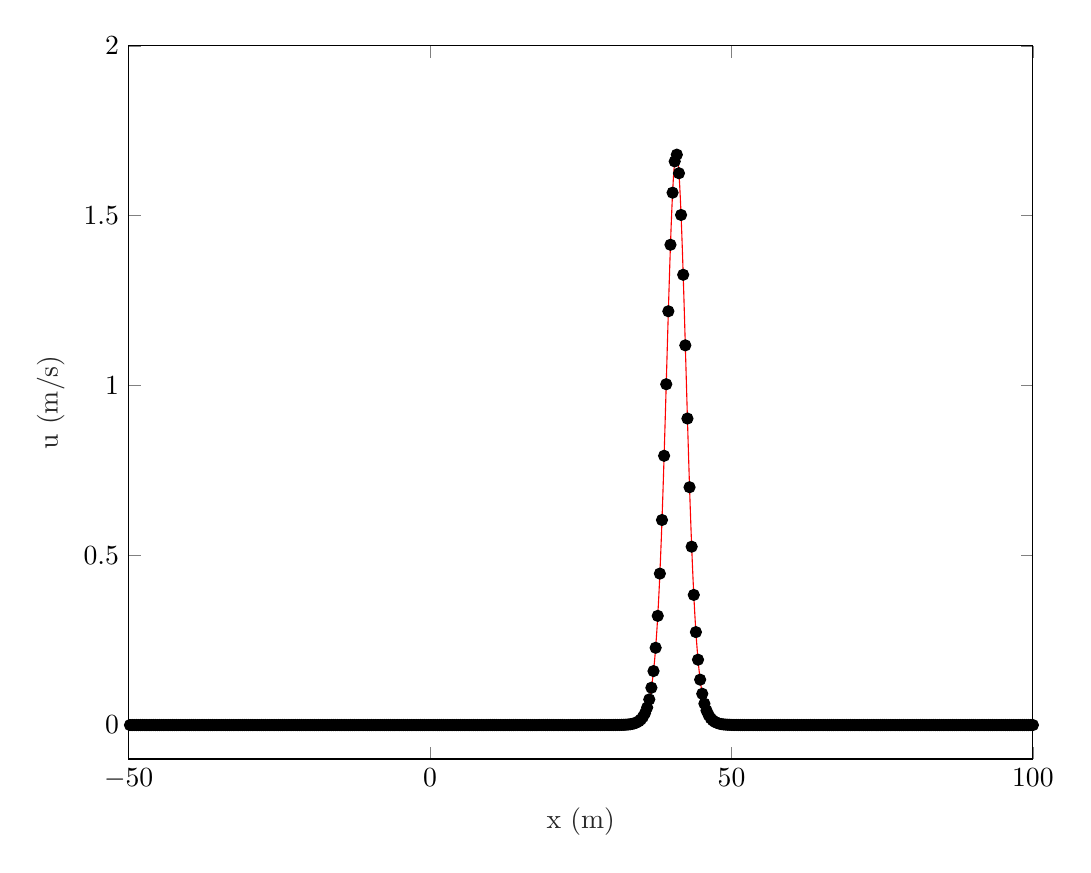
\begin{tikzpicture}

\begin{axis}[%
width=4.521in,
height=3.566in,
at={(0.758in,0.481in)},
scale only axis,
xmin=-50,
xmax=100,
xtick={-50,   0,  50, 100},
xlabel style={font=\color{white!15!black}},
xlabel={x (m)},
ymin=-0.1,
ymax=2,
ytick={  0, 0.5,   1, 1.5,   2},
ylabel style={font=\color{white!15!black}},
ylabel={u (m/s)},
axis background/.style={fill=white}
]
\addplot [color=red, forget plot]
  table[row sep=crcr]{%
-50.14064697609	0\\
-50.0234411626817	0\\
-49.9062353492733	0\\
-49.789029535865	0\\
-49.6718237224566	0\\
-49.5546179090483	0\\
-49.4374120956399	0\\
-49.3202062822316	0\\
-49.2030004688233	0\\
-49.0857946554149	0\\
-48.9685888420066	0\\
-48.8513830285982	0\\
-48.7341772151899	0\\
-48.6169714017815	0\\
-48.4997655883732	0\\
-48.3825597749648	0\\
-48.2653539615565	0\\
-48.1481481481481	0\\
-48.0309423347398	0\\
-47.9137365213315	0\\
-47.7965307079231	0\\
-47.6793248945148	0\\
-47.5621190811064	0\\
-47.4449132676981	0\\
-47.3277074542897	0\\
-47.2105016408814	0\\
-47.093295827473	0\\
-46.9760900140647	0\\
-46.8588842006564	0\\
-46.741678387248	0\\
-46.6244725738397	0\\
-46.5072667604313	0\\
-46.390060947023	0\\
-46.2728551336146	0\\
-46.1556493202063	0\\
-46.0384435067979	0\\
-45.9212376933896	0\\
-45.8040318799812	0\\
-45.6868260665729	0\\
-45.5696202531646	0\\
-45.4524144397562	0\\
-45.3352086263479	0\\
-45.2180028129395	0\\
-45.1007969995312	0\\
-44.9835911861228	0\\
-44.8663853727145	0\\
-44.7491795593061	0\\
-44.6319737458978	0\\
-44.5147679324894	0\\
-44.3975621190811	0\\
-44.2803563056728	0\\
-44.1631504922644	0\\
-44.0459446788561	0\\
-43.9287388654477	0\\
-43.8115330520394	0\\
-43.694327238631	0\\
-43.5771214252227	0\\
-43.4599156118143	0\\
-43.342709798406	0\\
-43.2255039849977	0\\
-43.1082981715893	0\\
-42.991092358181	0\\
-42.8738865447726	0\\
-42.7566807313643	0\\
-42.6394749179559	0\\
-42.5222691045476	0\\
-42.4050632911392	0\\
-42.2878574777309	0\\
-42.1706516643225	0\\
-42.0534458509142	0\\
-41.9362400375059	0\\
-41.8190342240975	0\\
-41.7018284106892	0\\
-41.5846225972808	0\\
-41.4674167838725	0\\
-41.3502109704641	0\\
-41.2330051570558	0\\
-41.1157993436474	0\\
-40.9985935302391	0\\
-40.8813877168308	0\\
-40.7641819034224	0\\
-40.6469760900141	0\\
-40.5297702766057	0\\
-40.4125644631974	0\\
-40.295358649789	0\\
-40.1781528363807	0\\
-40.0609470229723	0\\
-39.943741209564	0\\
-39.8265353961556	0\\
-39.7093295827473	0\\
-39.592123769339	0\\
-39.4749179559306	0\\
-39.3577121425223	0\\
-39.2405063291139	0\\
-39.1233005157056	0\\
-39.0060947022972	0\\
-38.8888888888889	0\\
-38.7716830754805	0\\
-38.6544772620722	0\\
-38.5372714486639	0\\
-38.4200656352555	0\\
-38.3028598218472	0\\
-38.1856540084388	0\\
-38.0684481950305	0\\
-37.9512423816221	0\\
-37.8340365682138	0\\
-37.7168307548054	0\\
-37.5996249413971	0\\
-37.4824191279887	0\\
-37.3652133145804	0\\
-37.2480075011721	0\\
-37.1308016877637	0\\
-37.0135958743554	0\\
-36.896390060947	0\\
-36.7791842475387	0\\
-36.6619784341303	0\\
-36.544772620722	0\\
-36.4275668073136	0\\
-36.3103609939053	0\\
-36.193155180497	0\\
-36.0759493670886	0\\
-35.9587435536803	0\\
-35.8415377402719	0\\
-35.7243319268636	0\\
-35.6071261134552	0\\
-35.4899203000469	0\\
-35.3727144866385	0\\
-35.2555086732302	0\\
-35.1383028598218	0\\
-35.0210970464135	0\\
-34.9038912330052	0\\
-34.7866854195968	0\\
-34.6694796061885	0\\
-34.5522737927801	0\\
-34.4350679793718	0\\
-34.3178621659634	0\\
-34.2006563525551	0\\
-34.0834505391467	0\\
-33.9662447257384	0\\
-33.8490389123301	0\\
-33.7318330989217	0\\
-33.6146272855134	0\\
-33.497421472105	0\\
-33.3802156586967	0\\
-33.2630098452883	0\\
-33.14580403188	0\\
-33.0285982184716	0\\
-32.9113924050633	0\\
-32.7941865916549	0\\
-32.6769807782466	0\\
-32.5597749648383	0\\
-32.4425691514299	0\\
-32.3253633380216	0\\
-32.2081575246132	0\\
-32.0909517112049	0\\
-31.9737458977965	0\\
-31.8565400843882	0\\
-31.7393342709798	0\\
-31.6221284575715	0\\
-31.5049226441632	0\\
-31.3877168307548	0\\
-31.2705110173465	0\\
-31.1533052039381	0\\
-31.0360993905298	0\\
-30.9188935771214	0\\
-30.8016877637131	0\\
-30.6844819503047	0\\
-30.5672761368964	0\\
-30.450070323488	0\\
-30.3328645100797	0\\
-30.2156586966714	0\\
-30.098452883263	0\\
-29.9812470698547	0\\
-29.8640412564463	0\\
-29.746835443038	0\\
-29.6296296296296	0\\
-29.5124238162213	0\\
-29.3952180028129	0\\
-29.2780121894046	0\\
-29.1608063759962	0\\
-29.0436005625879	0\\
-28.9263947491796	0\\
-28.8091889357712	0\\
-28.6919831223629	0\\
-28.5747773089545	0\\
-28.4575714955462	0\\
-28.3403656821378	0\\
-28.2231598687295	0\\
-28.1059540553211	0\\
-27.9887482419128	0\\
-27.8715424285045	0\\
-27.7543366150961	0\\
-27.6371308016878	0\\
-27.5199249882794	0\\
-27.4027191748711	0\\
-27.2855133614627	0\\
-27.1683075480544	0\\
-27.051101734646	0\\
-26.9338959212377	0\\
-26.8166901078293	0\\
-26.699484294421	0\\
-26.5822784810127	0\\
-26.4650726676043	0\\
-26.347866854196	0\\
-26.2306610407876	0\\
-26.1134552273793	0\\
-25.9962494139709	0\\
-25.8790436005626	0\\
-25.7618377871542	0\\
-25.6446319737459	0\\
-25.5274261603376	0\\
-25.4102203469292	0\\
-25.2930145335209	0\\
-25.1758087201125	0\\
-25.0586029067042	0\\
-24.9413970932958	0\\
-24.8241912798875	0\\
-24.7069854664791	0\\
-24.5897796530708	0\\
-24.4725738396624	0\\
-24.3553680262541	0\\
-24.2381622128458	0\\
-24.1209563994374	0\\
-24.0037505860291	0\\
-23.8865447726207	0\\
-23.7693389592124	0\\
-23.652133145804	0\\
-23.5349273323957	0\\
-23.4177215189873	0\\
-23.300515705579	0\\
-23.1833098921707	0\\
-23.0661040787623	0\\
-22.948898265354	0\\
-22.8316924519456	0\\
-22.7144866385373	0\\
-22.5972808251289	0\\
-22.4800750117206	0\\
-22.3628691983122	0\\
-22.2456633849039	0\\
-22.1284575714955	0\\
-22.0112517580872	0\\
-21.8940459446789	0\\
-21.7768401312705	0\\
-21.6596343178622	0\\
-21.5424285044538	0\\
-21.4252226910455	0\\
-21.3080168776371	0\\
-21.1908110642288	0\\
-21.0736052508204	0\\
-20.9563994374121	0\\
-20.8391936240038	0\\
-20.7219878105954	0\\
-20.6047819971871	0\\
-20.4875761837787	0\\
-20.3703703703704	0\\
-20.253164556962	0\\
-20.1359587435537	0\\
-20.0187529301453	0\\
-19.901547116737	0\\
-19.7843413033286	0\\
-19.6671354899203	0\\
-19.549929676512	0\\
-19.4327238631036	0\\
-19.3155180496953	0\\
-19.1983122362869	0\\
-19.0811064228786	0\\
-18.9639006094702	0\\
-18.8466947960619	0\\
-18.7294889826535	0\\
-18.6122831692452	0\\
-18.4950773558368	0\\
-18.3778715424285	0\\
-18.2606657290202	0\\
-18.1434599156118	0\\
-18.0262541022035	0\\
-17.9090482887951	0\\
-17.7918424753868	0\\
-17.6746366619784	0\\
-17.5574308485701	0\\
-17.4402250351617	0\\
-17.3230192217534	0\\
-17.2058134083451	0\\
-17.0886075949367	0\\
-16.9714017815284	0\\
-16.85419596812	0\\
-16.7369901547117	0\\
-16.6197843413033	0\\
-16.502578527895	0\\
-16.3853727144866	0\\
-16.2681669010783	0\\
-16.1509610876699	0\\
-16.0337552742616	0\\
-15.9165494608533	0\\
-15.7993436474449	0\\
-15.6821378340366	0\\
-15.5649320206282	0\\
-15.4477262072199	0\\
-15.3305203938115	0\\
-15.2133145804032	0\\
-15.0961087669948	0\\
-14.9789029535865	0\\
-14.8616971401782	0\\
-14.7444913267698	0\\
-14.6272855133615	0\\
-14.5100796999531	0\\
-14.3928738865448	0\\
-14.2756680731364	0\\
-14.1584622597281	0\\
-14.0412564463197	0\\
-13.9240506329114	0\\
-13.806844819503	0\\
-13.6896390060947	0\\
-13.5724331926864	0\\
-13.455227379278	0\\
-13.3380215658697	0\\
-13.2208157524613	0\\
-13.103609939053	0\\
-12.9864041256446	0\\
-12.8691983122363	0\\
-12.7519924988279	0\\
-12.6347866854196	0\\
-12.5175808720113	0\\
-12.4003750586029	0\\
-12.2831692451946	0\\
-12.1659634317862	0\\
-12.0487576183779	0\\
-11.9315518049695	0\\
-11.8143459915612	0\\
-11.6971401781528	0\\
-11.5799343647445	0\\
-11.4627285513361	0\\
-11.3455227379278	0\\
-11.2283169245195	0\\
-11.1111111111111	0\\
-10.9939052977028	0\\
-10.8766994842944	0\\
-10.7594936708861	0\\
-10.6422878574777	0\\
-10.5250820440694	0\\
-10.407876230661	0\\
-10.2906704172527	0\\
-10.1734646038444	0\\
-10.056258790436	0\\
-9.93905297702766	0\\
-9.82184716361932	0\\
-9.70464135021097	0\\
-9.58743553680262	0\\
-9.47022972339428	0\\
-9.35302390998594	0\\
-9.23581809657759	0\\
-9.11861228316924	0\\
-9.0014064697609	0\\
-8.88420065635255	0\\
-8.76699484294421	0\\
-8.64978902953587	0\\
-8.53258321612752	0\\
-8.41537740271917	0\\
-8.29817158931083	0\\
-8.18096577590249	0\\
-8.06375996249414	0\\
-7.94655414908579	0\\
-7.82934833567745	0\\
-7.7121425222691	0\\
-7.59493670886076	0\\
-7.47773089545242	0\\
-7.36052508204407	0\\
-7.24331926863572	0\\
-7.12611345522738	0\\
-7.00890764181904	0\\
-6.89170182841069	0\\
-6.77449601500234	0\\
-6.657290201594	0\\
-6.54008438818565	0\\
-6.42287857477731	0\\
-6.30567276136896	0\\
-6.18846694796062	0\\
-6.07126113455227	0\\
-5.95405532114393	0\\
-5.83684950773559	0\\
-5.71964369432724	0\\
-5.60243788091889	0\\
-5.48523206751055	0\\
-5.3680262541022	0\\
-5.25082044069386	0\\
-5.13361462728551	0\\
-5.01640881387717	0\\
-4.89920300046882	0\\
-4.78199718706048	0\\
-4.66479137365214	0\\
-4.54758556024379	0\\
-4.43037974683544	0\\
-4.31317393342709	0\\
-4.19596812001875	0\\
-4.07876230661041	0\\
-3.96155649320206	0\\
-3.84435067979372	0\\
-3.72714486638537	0\\
-3.60993905297703	0\\
-3.49273323956868	0\\
-3.37552742616034	0\\
-3.25832161275199	0\\
-3.14111579934364	0\\
-3.0239099859353	0\\
-2.90670417252696	0\\
-2.78949835911861	0\\
-2.67229254571027	0\\
-2.55508673230192	0\\
-2.43788091889358	0\\
-2.32067510548523	0\\
-2.20346929207689	0\\
-2.08626347866854	0\\
-1.96905766526019	0\\
-1.85185185185185	0\\
-1.73464603844351	0\\
-1.61744022503516	0\\
-1.50023441162681	0\\
-1.38302859821847	0\\
-1.26582278481013	0\\
-1.14861697140178	0\\
-1.03141115799344	0\\
-0.914205344585092	0\\
-0.796999531176745	0\\
-0.679793717768398	0\\
-0.562587904360058	0\\
-0.445382090951711	0\\
-0.328176277543363	0\\
-0.210970464135023	0\\
-0.0937646507266763	0\\
0.0234411626816708	0\\
0.140646976090011	0\\
0.257852789498358	0\\
0.375058602906705	0\\
0.492264416315052	0\\
0.609470229723392	0\\
0.726676043131739	0\\
0.843881856540087	0\\
0.961087669948427	0\\
1.07829348335677	0\\
1.19549929676512	0\\
1.31270511017347	0\\
1.42991092358181	0\\
1.54711673699016	0\\
1.6643225503985	0\\
1.78152836380684	0\\
1.89873417721519	0\\
2.01593999062354	0\\
2.13314580403188	0\\
2.25035161744022	0\\
2.36755743084857	0\\
2.48476324425692	0\\
2.60196905766526	0\\
2.71917487107361	0\\
2.83638068448195	0\\
2.95358649789029	0\\
3.07079231129864	0\\
3.18799812470699	0\\
3.30520393811533	0\\
3.42240975152367	0\\
3.53961556493202	0\\
3.65682137834037	0\\
3.77402719174871	0\\
3.89123300515705	0\\
4.0084388185654	0\\
4.12564463197375	0\\
4.24285044538209	0\\
4.36005625879044	0\\
4.47726207219878	0\\
4.59446788560712	0\\
4.71167369901547	0\\
4.82887951242382	0\\
4.94608532583216	0\\
5.0632911392405	0\\
5.18049695264885	0\\
5.2977027660572	0\\
5.41490857946554	0\\
5.53211439287389	0\\
5.64932020628223	0\\
5.76652601969058	0\\
5.88373183309892	0\\
6.00093764650727	0\\
6.11814345991561	0\\
6.23534927332395	0\\
6.3525550867323	0\\
6.46976090014065	0\\
6.58696671354899	0\\
6.70417252695734	0\\
6.82137834036568	0\\
6.93858415377403	9.06774273054312e-16\\
7.05578996718237	9.06774273054312e-16\\
7.17299578059072	9.06774273054312e-16\\
7.29020159399906	9.06774273054312e-16\\
7.4074074074074	9.06774273054312e-16\\
7.52461322081575	9.06774273054312e-16\\
7.6418190342241	9.06774273054312e-16\\
7.75902484763245	9.06774273054312e-16\\
7.87623066104079	1.81354854610862e-15\\
7.99343647444913	1.81354854610862e-15\\
8.11064228785748	1.81354854610862e-15\\
8.22784810126582	1.81354854610862e-15\\
8.34505391467417	2.72032281916294e-15\\
8.46225972808251	2.72032281916294e-15\\
8.57946554149086	2.72032281916294e-15\\
8.6966713548992	3.62709709221725e-15\\
8.81387716830755	3.62709709221725e-15\\
8.9310829817159	4.53387136527156e-15\\
9.04828879512424	5.44064563832587e-15\\
9.16549460853258	5.44064563832587e-15\\
9.28270042194093	6.34741991138018e-15\\
9.39990623534927	7.2541941844345e-15\\
9.51711204875762	9.06774273054312e-15\\
9.63431786216596	9.97451700359743e-15\\
9.75152367557431	1.08812912766517e-14\\
9.86872948898265	1.26948398227604e-14\\
9.985935302391	1.4508388368869e-14\\
10.1031411157993	1.63219369149776e-14\\
10.2203469292077	1.90422597341406e-14\\
10.337552742616	2.17625825533035e-14\\
10.4547585560244	2.44829053724664e-14\\
10.5719643694327	2.81100024646837e-14\\
10.6891701828411	3.17370995569009e-14\\
10.8063759962494	3.62709709221725e-14\\
10.9235818096578	4.0804842287444e-14\\
11.0407876230661	4.71522621988242e-14\\
11.1579934364744	5.34996821102044e-14\\
11.2751992498828	6.07538762946389e-14\\
11.3924050632911	6.89148447521277e-14\\
11.5096108766995	7.88893617557252e-14\\
11.6268166901078	8.97706530323769e-14\\
11.7440225035162	1.02465492855137e-13\\
11.8612283169245	1.16973881224006e-13\\
11.9784341303329	1.33295818138984e-13\\
12.0956399437412	1.5143130360007e-13\\
12.2128457571496	1.72287111880319e-13\\
12.3300515705579	1.96770017252786e-13\\
12.4472573839662	2.23973245444415e-13\\
12.5644631973746	2.54803570728262e-13\\
12.6816690107829	2.91074541650434e-13\\
12.7988748241913	3.30972609664824e-13\\
12.9160806375996	3.77218097590594e-13\\
13.033286451008	4.29811005427744e-13\\
13.1504922644163	4.89658107449328e-13\\
13.2676980778247	5.57666177928402e-13\\
13.384903891233	6.34741991138018e-13\\
13.5021097046413	7.23605869897341e-13\\
13.6193155180497	8.2425781420637e-13\\
13.736521331458	9.38511372611213e-13\\
13.8537271448664	1.06908686793103e-12\\
13.9709329582747	1.218704622985e-12\\
14.0881387716831	1.3873646377731e-12\\
14.2053445850914	1.58050755793367e-12\\
14.3225503984998	1.80085370628586e-12\\
14.4397562119081	2.05112340564885e-12\\
14.5569620253165	2.33675730166096e-12\\
14.6741678387248	2.66228926568746e-12\\
14.7913736521331	3.03225316909362e-12\\
14.9085794655415	3.45390320606387e-12\\
15.0257852789498	3.93449357078266e-12\\
15.1429910923582	4.48218523170746e-12\\
15.2601969057665	5.10604593156883e-12\\
15.3774027191749	5.81605018737036e-12\\
15.4946085325832	6.62579961320786e-12\\
15.6118143459916	7.54708227463104e-12\\
15.7290201593999	8.59712688282793e-12\\
15.8462259728083	9.79316214898657e-12\\
15.9634317862166	1.11560438813872e-11\\
16.0806375996249	1.27084414368562e-11\\
16.1978434130333	1.44766512693121e-11\\
16.3150492264416	1.64905969297657e-11\\
16.43225503985	1.87847358405931e-11\\
16.5494608532583	2.13980592955357e-11\\
16.6666666666667	2.4375906008246e-11\\
16.783872480075	2.77672417894691e-11\\
16.9010782934834	3.16301001926805e-11\\
17.0182841068917	3.60306757398131e-11\\
17.1354899203	4.10442306955304e-11\\
17.2526957337084	4.67541882929534e-11\\
17.3699015471167	5.3259386927845e-11\\
17.4871073605251	6.06695462872449e-11\\
17.6043131739334	6.91107079951074e-11\\
17.7215189873418	7.87261423865754e-11\\
17.8387248007501	8.96799756050715e-11\\
17.9559306141585	1.02157189602299e-10\\
18.0731364275668	1.16370876332425e-10\\
18.1903422409752	1.32562237752083e-10\\
18.3075480543835	1.51005119691735e-10\\
18.4247538677918	1.72015079598403e-10\\
18.5419596812002	1.95948479761398e-10\\
18.6591654946085	2.23210648280776e-10\\
18.7763713080169	2.54266760358614e-10\\
18.8935771214252	2.89643651847554e-10\\
19.0107829348336	3.29942514090634e-10\\
19.1279887482419	3.75847961664009e-10\\
19.2451945616503	4.28140727216778e-10\\
19.3624003750586	4.87708542762262e-10\\
19.4796061884669	5.55565181937735e-10\\
19.5968120018753	6.32862248069977e-10\\
19.7140178152836	7.20913657080643e-10\\
19.831223628692	8.21216493294545e-10\\
19.9484294421003	9.35474585570754e-10\\
20.0656352555087	1.06562933762788e-09\\
20.182841068917	1.2138923719179e-09\\
20.3000468823254	1.3827845209199e-09\\
20.4172526957337	1.57517481843383e-09\\
20.5344585091421	1.79433218571406e-09\\
20.6516643225504	2.04398255824855e-09\\
20.7688701359587	2.32836691931239e-09\\
20.8860759493671	2.65231837578095e-09\\
21.0032817627754	3.02134195426596e-09\\
21.1204875761838	3.44170890563984e-09\\
21.2376933895921	3.92056189085145e-09\\
21.3548992030005	4.46603920900146e-09\\
21.4721050164088	5.08741081348329e-09\\
21.5893108298172	5.79523427715812e-09\\
21.7065166432255	6.60153977430656e-09\\
21.8237224566338	7.52002866419446e-09\\
21.9409282700422	8.56630834560963e-09\\
22.0581340834505	9.7581597552724e-09\\
22.1753398968589	1.11158366033457e-08\\
22.2925457102672	1.26624108544331e-08\\
22.4097515236756	1.44241635472906e-08\\
22.5269573370839	1.64310327413173e-08\\
22.6441631504923	1.87171222169228e-08\\
22.7613689639006	2.13212818110619e-08\\
22.878574777309	2.42877648285823e-08\\
22.9957805907173	2.76669815716461e-08\\
23.1129864041256	3.151635578803e-08\\
23.230192217534	3.5901304894115e-08\\
23.3473980309423	4.0896341705628e-08\\
23.4646038443507	4.65863502690438e-08\\
23.581809657759	5.30680240055825e-08\\
23.6990154711674	6.04515087861918e-08\\
23.8162212845757	6.88622758738088e-08\\
23.9334270979841	7.84432546564492e-08\\
24.0506329113924	8.93572573616143e-08\\
24.1678387248007	1.01789751972017e-07\\
24.2850445382091	1.15952011452635e-07\\
24.4022503516174	1.32084700042954e-07\\
24.5194561650258	1.50461968249595e-07\\
24.6366619784341	1.71396111852519e-07\\
24.7538677918425	1.95242872907434e-07\\
24.8710736052508	2.2240749337084e-07\\
24.9882794186592	2.53351593436275e-07\\
25.1054852320675	2.88601021479201e-07\\
25.2226910454759	3.2875478759714e-07\\
25.3398968588842	3.74495244871209e-07\\
25.4571026722925	4.26599682475207e-07\\
25.5743084857009	4.85953536469996e-07\\
25.6915142991092	5.53565434548849e-07\\
25.8087201125176	6.30584339058476e-07\\
25.9259259259259	7.18319067128794e-07\\
26.0431317393343	8.18260536112787e-07\\
26.1603375527426	9.32107098406299e-07\\
26.277543366151	1.06179340089945e-06\\
26.3947491795593	1.20952326053126e-06\\
26.5119549929676	1.37780711769429e-06\\
26.629160806376	1.56950469452345e-06\\
26.7463666197843	1.78787358983615e-06\\
26.8635724331927	2.03662463996857e-06\\
26.980778246601	2.31998497313827e-06\\
27.0979840600094	2.64276984682245e-06\\
27.2151898734177	3.01046446917432e-06\\
27.3323956868261	3.42931721405818e-06\\
27.4496015002344	3.90644579388892e-06\\
27.5668073136428	4.44995821787938e-06\\
27.6840131270511	5.06909056369633e-06\\
27.8012189404594	5.77436392739224e-06\\
27.9184247538678	6.57776320528796e-06\\
28.0356305672761	7.49294074640665e-06\\
28.1528363806845	8.53544833888351e-06\\
28.2700421940928	9.72300147209892e-06\\
28.3872480075012	1.10757803598941e-05\\
28.5044538209095	1.26167728395292e-05\\
28.6216596343179	1.43721649746762e-05\\
28.7388654477262	1.63717859945929e-05\\
28.8560712611346	1.86496151297085e-05\\
28.9732770745429	2.12443589439223e-05\\
29.0904828879512	2.42001089776323e-05\\
29.2076887013596	2.7567090867513e-05\\
29.3248945147679	3.14025176564703e-05\\
29.4421003281763	3.57715617881077e-05\\
29.5593061415846	4.07484622794739e-05\\
29.676511954993	4.64177858754163e-05\\
29.7937177684013	5.28758635689993e-05\\
29.9109235818097	6.02324268779463e-05\\
30.028129395218	6.8612471626214e-05\\
30.1453352086263	7.81583808349547e-05\\
30.2625410220347	8.90323427240722e-05\\
30.379746835443	0.000101419104795608\\
30.4969526488514	0.00011552911067516\\
30.6141584622597	0.000131602072815669\\
30.7313642756681	0.000149911041553117\\
30.8485700890764	0.00017076703935599\\
30.9657759024848	0.000194524338611991\\
31.0829817158931	0.000221586472133703\\
31.2001875293015	0.000252413077847617\\
31.3173933427098	0.000287527693114307\\
31.4345991561181	0.000327526630003336\\
31.5518049695265	0.000373089080882208\\
31.6690107829348	0.000424988624155939\\
31.7862165963432	0.000484106323209475\\
31.9034224097515	0.000551445637959232\\
32.0206282231599	0.000628149398278317\\
32.1378340365682	0.000715519122346805\\
32.2550398499766	0.000815037001262058\\
32.3722456633849	0.000928390914450008\\
32.4894514767932	0.00105750288927762\\
32.6066572902016	0.00120456147328252\\
32.7238631036099	0.00137205854946016\\
32.8410689170183	0.00156283119467619\\
32.9582747304266	0.00178010925943831\\
33.075480543835	0.00202756943468269\\
33.1926863572433	0.00230939666879157\\
33.3098921706517	0.00263035390653889\\
33.42709798406	0.002995861241836\\
33.5443037974684	0.00341208570866381\\
33.6615096108767	0.00388604307979318\\
33.778715424285	0.00442571320104597\\
33.8959212376934	0.00504017055957566\\
34.0131270511017	0.00573973196690971\\
34.1303328645101	0.00653612342967975\\
34.2475386779184	0.00744266847969811\\
34.3647444913268	0.00847450043594509\\
34.4819503047351	0.00964880126703259\\
34.5991561181435	0.0109850699041282\\
34.7163619315518	0.0125054230078522\\
34.8335677449601	0.0142349312998318\\
34.9507735583685	0.0162019946063359\\
35.0679793717768	0.0184387586954479\\
35.1851851851852	0.0209815767790725\\
35.3023909985935	0.0238715181430804\\
35.4195968120019	0.0271549256952327\\
35.5368026254102	0.0308840231960466\\
35.6540084388186	0.0351175714574539\\
35.7712142522269	0.0399215707299474\\
35.8884200656353	0.0453700036984107\\
36.0056258790436	0.0515456097915298\\
36.122831692452	0.0585406766774211\\
36.2400375058603	0.066457828647872\\
36.3572433192686	0.0754107838569794\\
36.474449132677	0.0855250428609074\\
36.5916549460853	0.0969384594317847\\
36.7088607594937	0.109801631109072\\
36.826066572902	0.124278031483017\\
36.9432723863104	0.140543789101873\\
37.0604781997187	0.158786999845292\\
37.177684013127	0.179206441798467\\
37.2948898265354	0.202009545932535\\
37.4120956399437	0.22740946487397\\
37.5293014533521	0.255621079244283\\
37.6465072667604	0.28685579086935\\
37.7637130801688	0.321314979698232\\
37.8809188935771	0.359182051898698\\
37.9981247069855	0.400613085141572\\
38.1153305203938	0.445726186646318\\
38.2325363338022	0.494589819921988\\
38.3497421472105	0.547210521986804\\
38.4669479606189	0.603520612124091\\
38.5841537740272	0.663366666180676\\
38.7013595874355	0.72649967006103\\
38.8185654008439	0.792567840764187\\
38.9357712142522	0.861113081704344\\
39.0529770276606	0.931571897213825\\
39.1701828410689	1.00328132053016\\
39.2873886544773	1.07549002388592\\
39.4045944678856	1.14737431737289\\
39.5218002812939	1.21805826602\\
39.6390060947023	1.28663673549676\\
39.7562119081106	1.35219988723851\\
39.873417721519	1.41385753620772\\
39.9906235349273	1.47076187989757\\
40.1078293483357	1.52212738904434\\
40.225035161744	1.56724706833021\\
40.3422409751524	1.60550477611835\\
40.4594467885607	1.63638375643018\\
40.5766526019691	1.65947191363387\\
40.6938584153774	1.67446460119774\\
40.8110642287858	1.68116577729349\\
40.9282700421941	1.679488304982\\
41.0454758556024	1.66945396779611\\
41.1626816690108	1.65119347281564\\
41.2798874824191	1.62494637213412\\
41.3970932958275	1.59106050313487\\
41.5142991092358	1.54999028046363\\
41.6315049226442	1.50229301432615\\
41.7487107360525	1.44862241540816\\
41.8659165494608	1.38971859296451\\
41.9831223628692	1.32639415235617\\
42.1003281762775	1.25951641763248\\
42.2175339896859	1.18998628483471\\
42.3347398030942	1.11871467683508\\
42.4519456165026	1.04659794179064\\
42.5691514299109	0.974493748905007\\
42.6863572433193	0.903199049253638\\
42.8035630567276	0.833431484522666\\
42.920768870136	0.765815277425135\\
43.0379746835443	0.7008721862066\\
43.1551804969527	0.639017626126788\\
43.272386310361	0.580561623139842\\
43.3895921237693	0.525713922101334\\
43.5067979371777	0.474592352456931\\
43.624003750586	0.427233462682169\\
43.7412095639944	0.383604455121435\\
43.8584153774027	0.343615557468145\\
43.9756211908111	0.307132123716976\\
44.0928270042194	0.273985935762325\\
44.2100328176277	0.243985352652912\\
44.3272386310361	0.216924111204356\\
44.4444444444444	0.192588710024351\\
44.5616502578528	0.170764405960209\\
44.6788560712611	0.151239918856142\\
44.7960618846695	0.133810981268217\\
44.9132676980778	0.118282889593725\\
45.0304735114862	0.104472217262382\\
45.1476793248945	0.0922078440667746\\
45.2648851383029	0.0813314424334248\\
45.3820909517112	0.0716975446069546\\
45.4992967651196	0.0631732966348332\\
45.6165025785279	0.0556379872581005\\
45.7337083919362	0.0489824233049075\\
45.8509142053446	0.0431082084757877\\
45.9681200187529	0.0379269697156838\\
46.0853258321613	0.0333595646920224\\
46.2025316455696	0.0293352951160212\\
46.319737458978	0.0257911435615636\\
46.4369432723863	0.0226710458282338\\
46.5541490857947	0.0199252065352604\\
46.671354899203	0.0175094623067961\\
46.7885607126113	0.0153846944228922\\
46.9057665260197	0.01351629099686\\
47.022972339428	0.0118736574557193\\
47.1401781528364	0.0104297732277176\\
47.2573839662447	0.00916079198268795\\
47.3745897796531	0.00804568244945439\\
47.4917955930614	0.00706590668768253\\
47.6090014064698	0.00620513267114321\\
47.7262072198781	0.00544897810760407\\
47.8434130332865	0.00478478254886827\\
47.9606188466948	0.00420140501100139\\
48.0778246601031	0.00368904451347711\\
48.1950304735115	0.00323908114488455\\
48.3122362869198	0.00284393546359155\\
48.4294421003282	0.00249694423831388\\
48.5466479137365	0.00219225072204547\\
48.6638537271449	0.00192470783064548\\
48.7810595405532	0.00168979276311278\\
48.8982653539616	0.00148353175357757\\
49.0154711673699	0.00130243378515719\\
49.1326769807782	0.00114343222330498\\
49.2498827941866	0.00100383344171454\\
49.3670886075949	0.000881271617858047\\
49.4842944210033	0.000773668968633056\\
49.6015002344116	0.000679200780229493\\
49.71870604782	0.000596264660961034\\
49.8359118612283	0.000523453512314844\\
49.9531176746367	0.000459531772598186\\
50.070323488045	0.000403414540043558\\
50.1875293014534	0.000354149228735224\\
50.3047351148617	0.000310899451916122\\
50.42194092827	0.000272930863634315\\
50.5391467416784	0.000239598721858688\\
50.6563525550867	0.000210336964605091\\
50.7735583684951	0.000184648615646573\\
50.8907641819034	0.000162097358477567\\
51.0079699953118	0.000142300136678561\\
51.1251758087201	0.00012492065592359\\
51.2423816221285	0.000109663678018346\\
51.3595874355368	9.62700105928315e-05\\
51.4767932489451	8.45121077680922e-05\\
51.5939990623535	7.41902074147901e-05\\
51.7112048757618	6.51289396111296e-05\\
51.8284106891702	5.71743489067714e-05\\
51.9456165025785	5.01912799321048e-05\\
52.0628223159869	4.40610820660213e-05\\
52.1800281293952	3.86795942493338e-05\\
52.2972339428036	3.39553757725054e-05\\
52.4144397562119	2.98081530316197e-05\\
52.5316455696203	2.61674559040006e-05\\
52.6488513830286	2.29714206021477e-05\\
52.7660571964369	2.01657386928834e-05\\
52.8832630098453	1.77027344350346e-05\\
53.0004688232536	1.55405547838175e-05\\
53.117674636662	1.36424582934657e-05\\
53.2348804500703	1.19761908607231e-05\\
53.3520862634787	1.05134376963164e-05\\
53.469292076887	9.22934221546216e-06\\
53.5864978902954	8.10208369414741e-06\\
53.7037037037037	7.11250648867616e-06\\
53.820909517112	6.24379454632367e-06\\
53.9381153305204	5.48118566353429e-06\\
54.0553211439287	4.8117206426874e-06\\
54.1725269573371	4.22402307924488e-06\\
54.2897327707454	3.70810605334463e-06\\
54.4069385841538	3.25520241656744e-06\\
54.5241443975621	2.85761582161884e-06\\
54.6413502109705	2.50858993510192e-06\\
54.7585560243788	2.20219362674614e-06\\
54.8757618377872	1.93322018280707e-06\\
54.9929676511955	1.69709882847348e-06\\
55.1101734646038	1.48981705448983e-06\\
55.2273792780122	1.30785243362502e-06\\
55.3445850914205	1.1481127608755e-06\\
55.4617909048289	1.00788350952327e-06\\
55.5789967182372	8.8478170126165e-07\\
55.6962025316456	7.76715410563015e-07\\
55.8134083450539	6.81848216860387e-07\\
55.9306141584623	5.98567998817575e-07\\
56.0478199718706	5.25459535691138e-07\\
56.165025785279	4.61280461943597e-07\\
56.2822315986873	4.04940150737552e-07\\
56.3994374120956	3.55481184910186e-07\\
56.516643225504	3.1206308400216e-07\\
56.6338490389123	2.73948025283137e-07\\
56.7510548523207	2.40488298529712e-07\\
56.868260665729	2.11115308667032e-07\\
56.9854664791374	1.8532990320762e-07\\
57.1026722925457	1.6269390161951e-07\\
57.2198781059541	1.4282263756123e-07\\
57.3370839193624	1.25378428293497e-07\\
57.4542897327707	1.10064836611609e-07\\
57.5714955461791	9.66216314474252e-08\\
57.6887013595874	8.48203655312391e-08\\
57.8059071729958	7.44604934911119e-08\\
57.9231129864041	6.53659660087041e-08\\
58.0403187998125	5.7382233837078e-08\\
58.1575246132208	5.03736272230475e-08\\
58.2747304266292	4.42210449929443e-08\\
58.3919362400375	3.88199319926007e-08\\
58.5091420534459	3.40785054368727e-08\\
58.6263478668542	2.99161916307922e-08\\
58.7435536802625	2.62622594607382e-08\\
58.8607594936709	2.3054613477879e-08\\
58.9779653070792	2.02387474806614e-08\\
59.0951711204876	1.77668073635993e-08\\
59.2123769338959	1.55967877152675e-08\\
59.3295827473043	1.36918118395297e-08\\
59.4467885607126	1.20195088016119e-08\\
59.563994374121	1.05514575754739e-08\\
59.6812001875293	9.26271370763817e-09\\
59.7984060009376	8.13137587908768e-09\\
59.915611814346	7.13821775491085e-09\\
60.0328176277543	6.26636335911186e-09\\
60.1500234411627	5.500996000069e-09\\
60.267229254571	4.82910981438386e-09\\
60.3844350679794	4.23928760718441e-09\\
60.5016408813877	3.72150498888202e-09\\
60.6188466947961	3.26696443547954e-09\\
60.7360525082044	2.86794113694481e-09\\
60.8532583216128	2.51765332848966e-09\\
60.9704641350211	2.21014985056003e-09\\
61.0876699484294	1.94020405624603e-09\\
61.2048757618378	1.70322948127456e-09\\
61.3220815752461	1.49519914109899e-09\\
61.4392873886545	1.3125766160544e-09\\
61.5564932020628	1.15225983135267e-09\\
61.6736990154712	1.01152393030327e-09\\
61.7909048288795	8.87977749148169e-10\\
61.9081106422879	7.79521198670962e-10\\
62.0253164556962	6.84310806774532e-10\\
62.1425222691045	6.00729794930024e-10\\
62.2597280825129	5.27357247851561e-10\\
62.3769338959212	4.62946350913695e-10\\
62.4941397093296	4.06402627568847e-10\\
62.6113455227379	3.56764897087581e-10\\
62.7285513361463	3.13189859395956e-10\\
62.8457571495546	2.7493758668716e-10\\
62.962962962963	2.41357015033139e-10\\
63.0801687763713	2.11877783416144e-10\\
63.1973745897797	1.85999352437447e-10\\
63.314580403188	1.63281936574617e-10\\
63.4317862165964	1.4333834321306e-10\\
63.5489920300047	1.25831252323201e-10\\
63.666197843413	1.10462335169203e-10\\
63.7834036568214	9.69704407604281e-11\\
63.9006094702297	8.51270619800658e-11\\
64.0178152836381	7.4729081390952e-11\\
64.1350210970464	6.56023983326603e-11\\
64.2522269104548	5.75892340816794e-11\\
64.3694327238631	5.05553860455971e-11\\
64.4866385372714	4.43811600203702e-11\\
64.6038443506798	3.89604634160516e-11\\
64.7210501640881	3.42017120310625e-11\\
64.8382559774965	3.00242029551013e-11\\
64.9554617909048	2.63572077948697e-11\\
65.0726676043132	2.31381591255269e-11\\
65.1898734177215	2.03117437164166e-11\\
65.3070792311299	1.783080930534e-11\\
65.4242850445382	1.56527375014635e-11\\
65.5414908579466	1.3741257333865e-11\\
65.6586966713549	1.20628181544415e-11\\
65.7759024847633	1.05893099607283e-11\\
65.8931082981716	9.29624984735281e-12\\
66.0103141115799	8.16096845748881e-12\\
66.1275199249883	7.16442353140212e-12\\
66.2447257383966	6.28938635790471e-12\\
66.361931551805	5.52044177435465e-12\\
66.4791373652133	4.8467084894753e-12\\
66.5963431786217	4.25458488917083e-12\\
66.71354899203	3.73500323071071e-12\\
66.8307548054383	3.27889577136439e-12\\
66.9479606188467	2.87810154267439e-12\\
67.065166432255	2.52717989900237e-12\\
67.1823722456634	2.21796987189085e-12\\
67.2995780590717	1.94684436424761e-12\\
67.4167838724801	1.70926950470738e-12\\
67.5339896858884	1.50071142190489e-12\\
67.6511954992968	1.31754301874792e-12\\
67.7684013127051	1.15613719814425e-12\\
67.8856071261135	1.01558718582083e-12\\
68.0028129395218	8.91359110412389e-13\\
68.1200187529302	7.82546197645871e-13\\
68.2372245663385	6.86428124702114e-13\\
68.3544303797468	6.03004891581117e-13\\
68.4716361931552	5.29556175463718e-13\\
68.5888420065635	4.64268427803808e-13\\
68.7060478199719	4.0804842287444e-13\\
68.8232536333802	3.58175837856453e-13\\
68.9404594467886	3.14650672749846e-13\\
69.0576652601969	2.75659379008511e-13\\
69.1748710736052	2.42108730905501e-13\\
69.2920768870136	2.13091954167763e-13\\
69.4092827004219	1.86795500249188e-13\\
69.5264885138303	1.6412614342283e-13\\
69.6436943272386	1.44177109415636e-13\\
69.760900140647	1.26041623954549e-13\\
69.8781059540553	1.10626461312626e-13\\
69.9953117674637	9.70248472168114e-14\\
70.112517580872	8.52367816671053e-14\\
70.2297233942804	7.52622646635079e-14\\
70.3469292076887	6.61945219329648e-14\\
70.4641350210971	5.8033553475476e-14\\
70.5813408345054	5.07793592910415e-14\\
70.6985466479137	4.44319393796613e-14\\
70.8157524613221	3.89912937413354e-14\\
70.9329582747304	3.44574223760639e-14\\
71.0501640881388	2.99235510107923e-14\\
71.1673699015471	2.6296453918575e-14\\
71.2845757149555	2.35761310994121e-14\\
71.4017815283638	1.99490340071949e-14\\
71.5189873417721	1.81354854610862e-14\\
71.6361931551805	1.54151626419233e-14\\
71.7533989685888	1.36016140958147e-14\\
71.8706047819972	1.17880655497061e-14\\
71.9878105954055	1.08812912766517e-14\\
72.1050164088139	9.06774273054312e-15\\
72.2222222222222	8.16096845748881e-15\\
72.3394280356306	7.2541941844345e-15\\
72.4566338490389	6.34741991138018e-15\\
72.5738396624473	5.44064563832587e-15\\
72.6910454758556	4.53387136527156e-15\\
72.8082512892639	4.53387136527156e-15\\
72.9254571026723	3.62709709221725e-15\\
73.0426629160806	3.62709709221725e-15\\
73.159868729489	2.72032281916294e-15\\
73.2770745428973	2.72032281916294e-15\\
73.3942803563057	1.81354854610862e-15\\
73.511486169714	1.81354854610862e-15\\
73.6286919831224	1.81354854610862e-15\\
73.7458977965307	1.81354854610862e-15\\
73.8631036099391	9.06774273054312e-16\\
73.9803094233474	9.06774273054312e-16\\
74.0975152367557	9.06774273054312e-16\\
74.2147210501641	9.06774273054312e-16\\
74.3319268635724	9.06774273054312e-16\\
74.4491326769808	9.06774273054312e-16\\
74.5663384903891	9.06774273054312e-16\\
74.6835443037975	9.06774273054312e-16\\
74.8007501172058	9.06774273054312e-16\\
74.9179559306142	0\\
75.0351617440225	0\\
75.1523675574308	0\\
75.2695733708392	0\\
75.3867791842475	0\\
75.5039849976559	0\\
75.6211908110642	0\\
75.7383966244726	0\\
75.8556024378809	0\\
75.9728082512893	0\\
76.0900140646976	0\\
76.207219878106	0\\
76.3244256915143	0\\
76.4416315049226	0\\
76.558837318331	0\\
76.6760431317393	0\\
76.7932489451477	0\\
76.910454758556	0\\
77.0276605719644	0\\
77.1448663853727	0\\
77.2620721987811	0\\
77.3792780121894	0\\
77.4964838255977	0\\
77.6136896390061	0\\
77.7308954524144	0\\
77.8481012658228	0\\
77.9653070792311	0\\
78.0825128926395	0\\
78.1997187060478	0\\
78.3169245194562	0\\
78.4341303328645	0\\
78.5513361462729	0\\
78.6685419596812	0\\
78.7857477730896	0\\
78.9029535864979	0\\
79.0201593999062	0\\
79.1373652133146	0\\
79.2545710267229	0\\
79.3717768401313	0\\
79.4889826535396	0\\
79.606188466948	0\\
79.7233942803563	0\\
79.8406000937647	0\\
79.957805907173	0\\
80.0750117205813	0\\
80.1922175339897	0\\
80.309423347398	0\\
80.4266291608064	0\\
80.5438349742147	0\\
80.6610407876231	0\\
80.7782466010314	0\\
80.8954524144397	0\\
81.0126582278481	0\\
81.1298640412564	0\\
81.2470698546648	0\\
81.3642756680731	0\\
81.4814814814815	0\\
81.5986872948898	0\\
81.7158931082982	0\\
81.8330989217065	0\\
81.9503047351149	0\\
82.0675105485232	0\\
82.1847163619315	0\\
82.3019221753399	0\\
82.4191279887482	0\\
82.5363338021566	0\\
82.6535396155649	0\\
82.7707454289733	0\\
82.8879512423816	0\\
83.00515705579	0\\
83.1223628691983	0\\
83.2395686826067	0\\
83.356774496015	0\\
83.4739803094234	0\\
83.5911861228317	0\\
83.70839193624	0\\
83.8255977496484	0\\
83.9428035630567	0\\
84.0600093764651	0\\
84.1772151898734	0\\
84.2944210032818	0\\
84.4116268166901	0\\
84.5288326300985	0\\
84.6460384435068	0\\
84.7632442569152	0\\
84.8804500703235	0\\
84.9976558837318	0\\
85.1148616971402	0\\
85.2320675105485	0\\
85.3492733239569	0\\
85.4664791373652	0\\
85.5836849507735	0\\
85.7008907641819	0\\
85.8180965775902	0\\
85.9353023909986	0\\
86.0525082044069	0\\
86.1697140178153	0\\
86.2869198312236	0\\
86.404125644632	0\\
86.5213314580403	0\\
86.6385372714487	0\\
86.755743084857	0\\
86.8729488982653	0\\
86.9901547116737	0\\
87.107360525082	0\\
87.2245663384904	0\\
87.3417721518987	0\\
87.4589779653071	0\\
87.5761837787154	0\\
87.6933895921238	0\\
87.8105954055321	0\\
87.9278012189405	0\\
88.0450070323488	0\\
88.1622128457572	0\\
88.2794186591655	0\\
88.3966244725738	0\\
88.5138302859822	0\\
88.6310360993905	0\\
88.7482419127989	0\\
88.8654477262072	0\\
88.9826535396156	0\\
89.0998593530239	0\\
89.2170651664323	0\\
89.3342709798406	0\\
89.451476793249	0\\
89.5686826066573	0\\
89.6858884200656	0\\
89.803094233474	0\\
89.9203000468823	0\\
90.0375058602907	0\\
90.154711673699	0\\
90.2719174871074	0\\
90.3891233005157	0\\
90.506329113924	0\\
90.6235349273324	0\\
90.7407407407407	0\\
90.8579465541491	0\\
90.9751523675574	0\\
91.0923581809658	0\\
91.2095639943741	0\\
91.3267698077825	0\\
91.4439756211908	0\\
91.5611814345991	0\\
91.6783872480075	0\\
91.7955930614158	0\\
91.9127988748242	0\\
92.0300046882325	0\\
92.1472105016409	0\\
92.2644163150492	0\\
92.3816221284576	0\\
92.4988279418659	0\\
92.6160337552743	0\\
92.7332395686826	0\\
92.850445382091	0\\
92.9676511954993	0\\
93.0848570089076	0\\
93.202062822316	0\\
93.3192686357243	0\\
93.4364744491327	0\\
93.553680262541	0\\
93.6708860759494	0\\
93.7880918893577	0\\
93.9052977027661	0\\
94.0225035161744	0\\
94.1397093295828	0\\
94.2569151429911	0\\
94.3741209563995	0\\
94.4913267698078	0\\
94.6085325832161	0\\
94.7257383966245	0\\
94.8429442100328	0\\
94.9601500234412	0\\
95.0773558368495	0\\
95.1945616502579	0\\
95.3117674636662	0\\
95.4289732770745	0\\
95.5461790904829	0\\
95.6633849038912	0\\
95.7805907172996	0\\
95.8977965307079	0\\
96.0150023441163	0\\
96.1322081575246	0\\
96.2494139709329	0\\
96.3666197843413	0\\
96.4838255977496	0\\
96.601031411158	0\\
96.7182372245663	0\\
96.8354430379747	0\\
96.952648851383	0\\
97.0698546647914	0\\
97.1870604781997	0\\
97.3042662916081	0\\
97.4214721050164	0\\
97.5386779184248	0\\
97.6558837318331	0\\
97.7730895452414	0\\
97.8902953586498	0\\
98.0075011720581	0\\
98.1247069854665	0\\
98.2419127988748	0\\
98.3591186122832	0\\
98.4763244256915	0\\
98.5935302390999	0\\
98.7107360525082	0\\
98.8279418659166	0\\
98.9451476793249	0\\
99.0623534927333	0\\
99.1795593061416	0\\
99.2967651195499	0\\
99.4139709329583	0\\
99.5311767463666	0\\
99.648382559775	0\\
99.7655883731833	0\\
99.8827941865917	0\\
100	0\\
100.117205813408	0\\
};
\addplot [color=black, draw=none, mark=*, mark options={solid, black}, forget plot]
  table[row sep=crcr]{%
-50.14064697609	0\\
-49.789029535865	1.33338460333001e-10\\
-49.4374120956399	2.97683161924035e-10\\
-49.0857946554149	4.84780876856103e-10\\
-48.7341772151899	7.08589649035313e-10\\
-48.3825597749648	9.85435419619768e-10\\
-48.0309423347398	1.33507012041878e-09\\
-47.6793248945148	1.78186157475441e-09\\
-47.3277074542897	2.35621823842691e-09\\
-46.9760900140647	3.09630325640272e-09\\
-46.6244725738397	4.05011367185402e-09\\
-46.2728551336146	5.27799556116659e-09\\
-45.9212376933896	6.8556905156935e-09\\
-45.5696202531646	8.87801304854708e-09\\
-45.2180028129395	1.14632561792719e-08\\
-44.8663853727145	1.47584537692207e-08\\
-44.5147679324894	1.89456095541628e-08\\
-44.1631504922644	2.42490356714833e-08\\
-43.8115330520394	3.09438949927862e-08\\
-43.4599156118143	3.93660717777273e-08\\
-43.1082981715893	4.99234511427992e-08\\
-42.7566807313643	6.31086536333555e-08\\
-42.4050632911392	7.95132005682686e-08\\
-42.0534458509142	9.98430389391673e-08\\
-41.7018284106892	1.24935202213762e-07\\
-41.3502109704641	1.55775281964175e-07\\
-40.9985935302391	1.93515178161188e-07\\
-40.6469760900141	2.39490396952283e-07\\
-40.295358649789	2.95235878761624e-07\\
-39.943741209564	3.62499070013603e-07\\
-39.592123769339	4.43248560216823e-07\\
-39.2405063291139	5.39676269621797e-07\\
-38.8888888888889	6.54190759327367e-07\\
-38.5372714486639	7.89398858378004e-07\\
-38.1856540084388	9.48072452121548e-07\\
-37.8340365682138	1.13309701325416e-06\\
-37.4824191279887	1.34739832978536e-06\\
-37.1308016877637	1.59384397112592e-06\\
-36.7791842475387	1.87511638241896e-06\\
-36.4275668073136	2.19355524509088e-06\\
-36.0759493670886	2.5509679456184e-06\\
-35.7243319268636	2.9484087558802e-06\\
-35.3727144866385	3.385929730142e-06\\
-35.0210970464135	3.86230941634693e-06\\
-34.6694796061885	4.37476929970734e-06\\
-34.3178621659634	4.91869233540498e-06\\
-33.9662447257384	5.48736290383691e-06\\
-33.6146272855134	6.07175279017139e-06\\
-33.2630098452883	6.66038287283543e-06\\
-32.9113924050633	7.23929472843268e-06\\
-32.5597749648383	7.7921694811506e-06\\
-32.2081575246132	8.30063221076705e-06\\
-31.8565400843882	8.74477803881816e-06\\
-31.5049226441632	9.10394964867292e-06\\
-31.1533052039381	9.35778440107857e-06\\
-30.8016877637131	9.48753156271414e-06\\
-30.450070323488	9.47761270555105e-06\\
-30.098452883263	9.31738941513813e-06\\
-29.746835443038	9.00300502242732e-06\\
-29.3952180028129	8.53921976175087e-06\\
-29.0436005625879	7.94103299954517e-06\\
-28.6919831223629	7.2348936186109e-06\\
-28.3403656821378	6.45925780893397e-06\\
-27.9887482419128	5.66424312787201e-06\\
-27.6371308016878	4.91013963788634e-06\\
-27.2855133614627	4.26458294370341e-06\\
-26.9338959212377	3.79827679022336e-06\\
-26.5822784810127	3.57927856404587e-06\\
-26.2306610407876	3.6660373891874e-06\\
-25.8790436005626	4.09953103192624e-06\\
-25.5274261603376	4.89521633880276e-06\\
-25.1758087201125	6.03552120980725e-06\\
-24.8241912798875	7.46400492920237e-06\\
-24.4725738396624	9.08233086174378e-06\\
-24.1209563994374	1.07512386061004e-05\\
-23.7693389592124	1.22965473827971e-05\\
-23.4177215189873	1.35208711263208e-05\\
-23.0661040787623	1.42211551585144e-05\\
-22.7144866385373	1.42113457850028e-05\\
-22.3628691983122	1.33486669822111e-05\\
-22.0112517580872	1.15606662919009e-05\\
-21.6596343178622	8.86968860553053e-06\\
-21.3080168776371	5.41037826320181e-06\\
-20.9563994374121	1.43578881469432e-06\\
-20.6047819971871	-2.69188807627503e-06\\
-20.253164556962	-6.5286387687305e-06\\
-19.901547116737	-9.59443239839944e-06\\
-19.549929676512	-1.14349347720072e-05\\
-19.1983122362869	-1.16929742521157e-05\\
-18.8466947960619	-1.01804136466077e-05\\
-18.4950773558368	-6.93745537747186e-06\\
-18.1434599156118	-2.2664873880967e-06\\
-17.7918424753868	3.27238205904421e-06\\
-17.4402250351617	8.91225734259901e-06\\
-17.0886075949367	1.37780552277431e-05\\
-16.7369901547117	1.70244119861747e-05\\
-16.3853727144866	1.79938835555958e-05\\
-16.0337552742616	1.63674358908694e-05\\
-15.6821378340366	1.22730124369411e-05\\
-15.3305203938115	6.31954067837748e-06\\
-14.9789029535865	-4.66459827786461e-07\\
-14.6272855133615	-6.8071375427286e-06\\
-14.2756680731364	-1.14228685091052e-05\\
-13.9240506329114	-1.33197074966286e-05\\
-13.5724331926864	-1.20487428815103e-05\\
-13.2208157524613	-7.86586971660065e-06\\
-12.8691983122363	-1.72889784779393e-06\\
-12.5175808720113	4.89042874755737e-06\\
-12.1659634317862	1.03570033485027e-05\\
-11.8143459915612	1.33053995705225e-05\\
-11.4627285513361	1.30348254866004e-05\\
-11.1111111111111	9.73855177098587e-06\\
-10.7594936708861	4.47093027824887e-06\\
-10.407876230661	-1.16108560149178e-06\\
-10.056258790436	-5.50247978588365e-06\\
-9.70464135021097	-7.38542093395537e-06\\
-9.35302390998594	-6.50065063271628e-06\\
-9.0014064697609	-3.45877861838807e-06\\
-8.64978902953587	4.88860884639841e-07\\
-8.29817158931083	3.95180248194184e-06\\
-7.94655414908579	5.90999997420874e-06\\
-7.59493670886076	6.01565401880961e-06\\
-7.24331926863572	4.58507948615589e-06\\
-6.89170182841069	2.34086155445585e-06\\
-6.54008438818565	8.3484099356668e-08\\
-6.18846694796062	-1.54164800891977e-06\\
-5.83684950773559	-2.13994513579281e-06\\
-5.48523206751055	-1.60542164304645e-06\\
-5.13361462728551	-1.75206193087525e-07\\
-4.78199718706048	1.55557340646471e-06\\
-4.43037974683544	2.80792776510332e-06\\
-4.07876230661041	3.01060369527548e-06\\
-3.72714486638537	2.16761931763061e-06\\
-3.37552742616034	8.6323669531977e-07\\
-3.0239099859353	-1.51322496199073e-07\\
-2.67229254571027	-4.42385460057819e-07\\
-2.32067510548523	-6.76488720261088e-08\\
-1.96905766526019	6.19124820139388e-07\\
-1.61744022503516	1.25945939480123e-06\\
-1.26582278481013	1.59859610850754e-06\\
-0.914205344585092	1.43978048622033e-06\\
-0.562587904360058	7.65155586848382e-07\\
-0.210970464135023	1.5111471142476e-07\\
0.140646976090011	5.06466123961307e-07\\
0.492264416315052	9.72559718048777e-07\\
0.843881856540087	-3.66260039581897e-07\\
1.19549929676512	2.52593316886242e-06\\
1.54711673699016	-8.97240389414172e-07\\
1.89873417721519	2.11841862850306e-06\\
2.25035161744022	2.89815507368055e-06\\
2.60196905766526	-2.92939859289772e-06\\
2.95358649789029	-1.45517892091045e-06\\
3.30520393811533	2.53665270503579e-06\\
3.65682137834037	2.86250263104739e-06\\
4.0084388185654	9.17549263987616e-07\\
4.36005625879044	3.88238121310314e-07\\
4.71167369901547	1.50438412555082e-06\\
5.0632911392405	1.65979269698056e-06\\
5.41490857946554	-6.66013063674313e-07\\
5.76652601969058	-3.8489196101008e-06\\
6.11814345991561	-4.57148815642802e-06\\
6.46976090014065	-8.5527678376652e-07\\
6.82137834036568	5.98596134761942e-06\\
7.17299578059072	1.18085001616355e-05\\
7.52461322081575	1.21128199733487e-05\\
7.87623066104079	5.00978989529216e-06\\
8.22784810126582	-7.09699600723886e-06\\
8.57946554149086	-1.82554646713343e-05\\
8.9310829817159	-2.19066691412211e-05\\
9.28270042194093	-1.44927089019543e-05\\
9.63431786216596	2.26370213678297e-06\\
9.985935302391	2.17160422376225e-05\\
10.337552742616	3.51531109605485e-05\\
10.6891701828411	3.5743194667307e-05\\
11.0407876230661	2.16723176047534e-05\\
11.3924050632911	-2.90744228276169e-06\\
11.7440225035162	-2.94435851524277e-05\\
12.0956399437412	-4.82532914900231e-05\\
12.4472573839662	-5.21040870541994e-05\\
12.7988748241913	-3.87344314533261e-05\\
13.1504922644163	-1.1522738508942e-05\\
13.5021097046413	2.17664233108984e-05\\
13.8537271448664	5.15275174257327e-05\\
14.2053445850914	6.92210581797928e-05\\
14.5569620253165	6.97283963718468e-05\\
14.9085794655415	5.25445026800695e-05\\
15.2601969057665	2.16374647334924e-05\\
15.6118143459916	-1.58264106320662e-05\\
15.9634317862166	-5.14001671304291e-05\\
16.3150492264416	-7.73663631481213e-05\\
16.6666666666667	-8.83562148743366e-05\\
17.0182841068917	-8.22726577193526e-05\\
17.3699015471167	-6.04256687277781e-05\\
17.7215189873418	-2.69755655497294e-05\\
18.0731364275668	1.20983117809022e-05\\
18.4247538677918	5.02235567137054e-05\\
18.7763713080169	8.13995328994789e-05\\
19.1279887482419	0.000101103928509701\\
19.4796061884669	0.000106830380149672\\
19.831223628692	9.82309767942453e-05\\
20.182841068917	7.69190664709327e-05\\
20.5344585091421	4.60137341586153e-05\\
20.8860759493671	9.54866986732589e-06\\
21.2376933895921	-2.8146937308462e-05\\
21.5893108298172	-6.30031691085769e-05\\
21.9409282700422	-9.16398219744765e-05\\
22.2925457102672	-0.000111641202414316\\
22.6441631504923	-0.000121672049906627\\
22.9957805907173	-0.00012145286403121\\
23.3473980309423	-0.000111625995859635\\
23.6990154711674	-9.35527147025921e-05\\
24.0506329113924	-6.90746597200956e-05\\
24.4022503516174	-4.02755350928353e-05\\
24.7538677918425	-9.26603568936536e-06\\
25.1054852320675	2.19916641545095e-05\\
25.4571026722925	5.18120442714712e-05\\
25.8087201125176	7.88661596796757e-05\\
26.1603375527426	0.00010221774593123\\
26.5119549929676	0.000121323570216104\\
26.8635724331927	0.000136007890588552\\
27.2151898734177	0.000146421567512505\\
27.5668073136428	0.000152996152810016\\
27.9184247538678	0.000156403012351134\\
28.2700421940928	0.00015752637873783\\
28.6216596343179	0.000157460003762371\\
28.9732770745429	0.000157537379828985\\
29.3248945147679	0.000159408065331927\\
29.676511954993	0.000165177390956274\\
30.028129395218	0.000177634047744857\\
30.379746835443	0.000200601630226612\\
30.7313642756681	0.00023946837018136\\
31.0829817158931	0.000301975172560501\\
31.4345991561181	0.000399381401682303\\
31.7862165963432	0.000548185394763086\\
32.1378340365682	0.000772661124021514\\
32.4894514767932	0.00110859609368907\\
32.8410689170183	0.00160879573018789\\
33.1926863572433	0.00235118032036556\\
33.5443037974684	0.00345067420976741\\
33.8959212376934	0.00507661379726201\\
34.2475386779184	0.00747812467473998\\
34.5991561181435	0.0110208703437883\\
34.9507735583685	0.0162397313646728\\
35.3023909985935	0.023913155322768\\
35.6540084388186	0.0351655747242331\\
36.0056258790436	0.0516030757412987\\
36.3572433192686	0.0754815250080598\\
36.7088607594937	0.109890130259016\\
37.0604781997187	0.158898096918303\\
37.4120956399437	0.227547624153226\\
37.7637130801688	0.321483118047236\\
38.1153305203938	0.445924474351723\\
38.4669479606189	0.603746298023641\\
38.8185654008439	0.792817118673329\\
39.1701828410689	1.00355209353713\\
39.5218002812939	1.21834919771698\\
39.873417721519	1.41415945831959\\
40.225035161744	1.56753071553904\\
40.5766526019691	1.6596828370047\\
40.9282700421941	1.67955967215572\\
41.2798874824191	1.6248071278677\\
41.6315049226442	1.50192145874534\\
41.9831223628692	1.32582511212789\\
42.3347398030942	1.11803175882983\\
42.6863572433193	0.902502532105264\\
43.0379746835443	0.70024305133121\\
43.3895921237693	0.5251954251378\\
43.7412095639944	0.383205054295822\\
44.0928270042194	0.273692789085065\\
44.4444444444444	0.192380685949561\\
44.7960618846695	0.133666743006399\\
45.1476793248945	0.0921094004933563\\
45.4992967651196	0.0631068275769737\\
45.8509142053446	0.0430636583783803\\
46.2025316455696	0.0293055881411815\\
46.5541490857947	0.0199054685396702\\
46.9057665260197	0.0135032107593485\\
47.2573839662447	0.00915214068746264\\
47.6090014064698	0.00619941939575142\\
47.9606188466948	0.00419763670175195\\
48.3122362869198	0.00284145267892262\\
48.6638537271449	0.0019230736278294\\
49.0154711673699	0.0013013591288934\\
49.3670886075949	0.000880565564113807\\
49.71870604782	0.000595801205402249\\
50.070323488045	0.000403110612087593\\
50.42194092827	0.000272731745985402\\
50.7735583684951	0.00018451829744477\\
51.1251758087201	0.000124835457366575\\
51.4767932489451	8.44564708499167e-05\\
51.8284106891702	5.71380606865588e-05\\
52.1800281293952	3.86559566021621e-05\\
52.5316455696203	2.61520800695171e-05\\
52.8832630098453	1.76927476828345e-05\\
53.2348804500703	1.1969714801676e-05\\
53.5864978902954	8.09789149363538e-06\\
53.9381153305204	5.47847700698863e-06\\
54.2897327707454	3.70635952694811e-06\\
54.6413502109705	2.50746630778487e-06\\
54.9929676511955	1.69637771945165e-06\\
55.3445850914205	1.14765123033039e-06\\
55.6962025316456	7.76420904722807e-07\\
56.0478199718706	5.25272239266963e-07\\
56.3994374120956	3.55362517696208e-07\\
56.7510548523207	2.40413432374381e-07\\
57.1026722925457	1.62646898212157e-07\\
57.4542897327707	1.10035492490217e-07\\
57.8059071729958	7.44422919045005e-08\\
58.1575246132208	5.03624240407031e-08\\
58.5091420534459	3.40716738487044e-08\\
58.8607594936709	2.30504960266635e-08\\
59.2123769338959	1.55943412587129e-08\\
59.563994374121	1.05500298972171e-08\\
59.915611814346	7.13740328482286e-09\\
60.267229254571	4.82865955342946e-09\\
60.6188466947961	3.26672901355118e-09\\
60.9704641350211	2.21003698529753e-09\\
61.3220815752461	1.49515312322148e-09\\
61.6736990154712	1.01151299941455e-09\\
62.0253164556962	6.84316859708497e-10\\
62.3769338959212	4.62959653876683e-10\\
62.7285513361463	3.1320468677996e-10\\
63.0801687763713	2.1189060375864e-10\\
63.4317862165964	1.4334776924921e-10\\
63.7834036568214	9.69746749057455e-11\\
64.1350210970464	6.56014378382334e-11\\
64.4866385372714	4.43758147236879e-11\\
64.8382559774965	3.00151205186676e-11\\
65.1898734177215	2.02989530847071e-11\\
65.5414908579466	1.37252951033395e-11\\
65.8931082981716	9.27785881117845e-12\\
66.2447257383966	6.26868289800291e-12\\
66.5963431786217	4.23293285990774e-12\\
66.9479606188467	2.8559661972924e-12\\
67.2995780590717	1.92436607486338e-12\\
67.6511954992968	1.29359752940449e-12\\
68.0028129395218	8.66425773849346e-13\\
68.3544303797468	5.7703314610401e-13\\
68.7060478199719	3.81084563217604e-13\\
69.0576652601969	2.48790289699558e-13\\
69.4092827004219	1.59803308822346e-13\\
69.760900140647	1.00241397692199e-13\\
70.112517580872	6.05766916283951e-14\\
70.4641350210971	3.47860386229237e-14\\
70.8157524613221	1.90326435651417e-14\\
71.1673699015471	1.03519834535999e-14\\
71.5189873417721	5.63051375689482e-15\\
71.8706047819972	3.06247448217831e-15\\
72.2222222222222	1.66570056640189e-15\\
72.5738396624473	9.05985794512825e-16\\
72.9254571026723	4.92771796093029e-16\\
73.2770745428973	2.68021909941009e-16\\
73.6286919831224	1.45778928051444e-16\\
73.9803094233474	7.92901441098806e-17\\
74.3319268635724	4.31264452071361e-17\\
74.6835443037975	2.34567649874197e-17\\
75.0351617440225	1.27582929924397e-17\\
75.3867791842475	6.93932177639307e-18\\
75.7383966244726	3.77434400862703e-18\\
76.0900140646976	2.05289121249878e-18\\
76.4416315049226	1.11658140347619e-18\\
76.7932489451477	6.0731617096812e-19\\
77.1448663853727	3.30323369501866e-19\\
77.4964838255977	1.79665112926483e-19\\
77.8481012658228	9.77210690589769e-20\\
78.1997187060478	5.31511498391837e-20\\
78.5513361462729	2.89092695815922e-20\\
78.9029535864979	1.57239470880656e-20\\
79.2545710267229	8.55236108025773e-21\\
79.606188466948	4.65168698657235e-21\\
79.957805907173	2.53008398709874e-21\\
80.309423347398	1.37612977834744e-21\\
80.6610407876231	7.48486286032788e-22\\
81.0126582278481	4.07106749082871e-22\\
81.3642756680731	2.21428111966186e-22\\
81.7158931082982	1.20436246462054e-22\\
82.0675105485232	6.55060883330095e-23\\
82.4191279887482	3.56292041204061e-23\\
82.7707454289733	1.93789648956015e-23\\
83.1223628691983	1.05403499656022e-23\\
83.4739803094234	5.73296757571331e-24\\
83.8255977496484	3.1181998065946e-24\\
84.1772151898734	1.69600994693169e-24\\
84.5288326300985	9.2247127140727e-25\\
84.8804500703235	5.01738358381231e-25\\
85.2320675105485	2.72898883763665e-25\\
85.5836849507735	1.48431547071129e-25\\
85.9353023909986	8.0732921520517e-26\\
86.2869198312236	4.39111815907612e-26\\
86.6385372714487	2.38835884095534e-26\\
86.9901547116737	1.29904451361193e-26\\
87.3417721518987	7.06559089617475e-27\\
87.6933895921238	3.84302263617589e-27\\
88.0450070323488	2.09024598213803e-27\\
88.3966244725738	1.13689891511849e-27\\
88.7482419127989	6.18367002851748e-28\\
89.0998593530239	3.36333991642521e-28\\
89.451476793249	1.82934330927279e-28\\
89.803094233474	9.94992188222834e-29\\
90.154711673699	5.41182975118004e-29\\
90.506329113924	2.94353077365047e-29\\
90.8579465541491	1.60100627953752e-29\\
91.2095639943741	8.7079813469716e-30\\
91.5611814345991	4.73632990128575e-30\\
91.9127988748242	2.57612184040886e-30\\
92.2644163150492	1.40117007787463e-30\\
92.6160337552743	7.62105874158736e-31\\
92.9676511954993	4.1451453509573e-31\\
93.3192686357243	2.25457256825763e-31\\
93.6708860759494	1.22627725555291e-31\\
94.0225035161744	6.66980485772742e-32\\
94.3741209563995	3.6277519271208e-32\\
94.7257383966245	1.97315877382556e-32\\
95.0773558368495	1.07321436386508e-32\\
95.4289732770745	5.83728494678491e-33\\
95.7805907172996	3.17493780341325e-33\\
96.1322081575246	1.726868423846e-33\\
96.4838255977496	9.39252274524075e-34\\
96.8354430379747	5.10859902855756e-34\\
97.1870604781997	2.77849569786806e-34\\
97.5386779184248	1.51104800065923e-34\\
97.8902953586498	8.21511462928677e-35\\
98.2419127988748	4.46167883898779e-35\\
98.5935302390999	2.41464416230967e-35\\
98.9451476793249	1.29110748632998e-35\\
99.2967651195499	6.61364140615643e-36\\
99.648382559775	2.84564260081771e-36\\
100	1.6598024421102e-37\\
};
\end{axis}
\end{tikzpicture}%
		\caption{$t = 10s$}
	\end{subfigure}
	\begin{subfigure}{0.49\textwidth}
		\centering
		% This file was created by matlab2tikz.
%
%The latest updates can be retrieved from
%  http://www.mathworks.com/matlabcentral/fileexchange/22022-matlab2tikz-matlab2tikz
%where you can also make suggestions and rate matlab2tikz.
%
\begin{tikzpicture}

\begin{axis}[%
width=4.521in,
height=3.566in,
at={(0.758in,0.481in)},
scale only axis,
xmin=-50,
xmax=100,
xtick={-50,   0,  50, 100},
xlabel style={font=\color{white!15!black}},
xlabel={x (m)},
ymin=-0.1,
ymax=0.4,
ytick={-0.1,    0,  0.1,  0.2,  0.3,  0.4},
ylabel style={font=\color{white!15!black}},
ylabel={$\text{G (m}^\text{2}\text{/s)}$},
axis background/.style={fill=white}
]
\addplot [color=green!60!black, forget plot]
  table[row sep=crcr]{%
-50.2813379180994	1.06511867902256e-28\\
-50.0468896530166	1.91770795785705e-28\\
-49.8124413879337	3.44328815498068e-28\\
-49.5779931228509	6.16553397781048e-28\\
-49.3435448577681	1.10096737841321e-27\\
-49.1090965926852	1.96058030376556e-27\\
-48.8746483276024	3.48177937527298e-27\\
-48.6402000625195	6.16629488984274e-27\\
-48.4057517974367	1.08906489837559e-26\\
-48.1713035323539	1.91818133035259e-26\\
-47.936855267271	3.36924030658023e-26\\
-47.7024070021882	5.90174912275146e-26\\
-47.4679587371053	1.03094602732762e-25\\
-47.2335104720225	1.7959636544979e-25\\
-46.9990622069397	3.12007896947607e-25\\
-46.7646139418568	5.40555210117238e-25\\
-46.530165676774	9.33944261088278e-25\\
-46.2957174116912	1.60919356298529e-24\\
-46.0612691466083	2.76504398500092e-24\\
-45.8268208815255	4.73807826818525e-24\\
-45.5923726164426	8.09671486846486e-24\\
-45.3579243513598	1.37981826427862e-23\\
-45.123476086277	2.34499197992297e-23\\
-44.8890278211941	3.9743605460156e-23\\
-44.6545795561113	6.71737498649184e-23\\
-44.4201312910284	1.13223962895879e-22\\
-44.1856830259456	1.9031960980691e-22\\
-43.9512347608628	3.19032667155935e-22\\
-43.7167864957799	5.33326544059875e-22\\
-43.4823382306971	8.89114458826703e-22\\
-43.2478899656143	1.47818426498979e-21\\
-43.0134417005314	2.45078890661194e-21\\
-42.7789934354486	4.05218874010792e-21\\
-42.5445451703657	6.68159047799637e-21\\
-42.3100969052829	1.09869328638068e-20\\
-42.0756486402001	1.80168771168438e-20\\
-41.8412003751172	2.94638158104609e-20\\
-41.6067521100344	4.80512725964258e-20\\
-41.3723038449515	7.814968393912e-20\\
-41.1378555798687	1.26752340247965e-19\\
-40.9034073147859	2.05017614444583e-19\\
-40.668959049703	3.30698933130689e-19\\
-40.4345107846202	5.31962282227611e-19\\
-40.2000625195374	8.53365961477725e-19\\
-39.9656142544545	1.36519981313145e-18\\
-39.7311659893717	2.17802847357435e-18\\
-39.4967177242888	3.46527188191608e-18\\
-39.262269459206	5.49816165809859e-18\\
-39.0278211941232	8.69969693986612e-18\\
-38.7933729290403	1.37276807800934e-17\\
-38.5589246639575	2.16021336207052e-17\\
-38.3244763988747	3.39002228587555e-17\\
-38.0900281337918	5.30536034736352e-17\\
-37.855579868709	8.28006316232122e-17\\
-37.6211316036261	1.28872080859125e-16\\
-37.3866833385433	2.00027847259712e-16\\
-37.1522350734605	3.09619645984697e-16\\
-36.9177868083776	4.77939568538012e-16\\
-36.6833385432948	7.35739195887744e-16\\
-36.4488902782119	1.12948697787813e-15\\
-36.2144420131291	1.72919906401222e-15\\
-35.9799937480463	2.64006843150931e-15\\
-35.7455454829634	4.01968299967566e-15\\
-35.5110972178806	6.10344246265523e-15\\
-35.2766489527977	9.24196529324532e-15\\
-35.0422006877149	1.39559768513142e-14\\
-34.8077524226321	2.10166056965791e-14\\
-34.5733041575492	3.15624960322436e-14\\
-34.3388558924664	4.72701014268869e-14\\
-34.1044076273836	7.06005616758623e-14\\
-33.8699593623007	1.05156520378949e-13\\
-33.6355110972179	1.56196279969865e-13\\
-33.401062832135	2.31372422909919e-13\\
-33.1666145670522	3.417896688814e-13\\
-32.9321663019694	5.03515329246521e-13\\
-32.6977180368865	7.39729419561772e-13\\
-32.4632697718037	1.08377596215715e-12\\
-32.2288215067208	1.58347994003909e-12\\
-31.994373241638	2.30723614340874e-12\\
-31.7599249765552	3.35257078046572e-12\\
-31.5254767114723	4.85814299190808e-12\\
-31.2910284463895	7.02051642947149e-12\\
-31.0565801813067	1.01175242808807e-11\\
-30.8221319162238	1.45407189185515e-11\\
-30.587683651141	2.08402983509207e-11\\
-30.3532353860581	2.97871130373142e-11\\
-30.1187871209753	4.24579795618744e-11\\
-29.8843388558925	6.03526942479265e-11\\
-29.6498905908096	8.55540218077207e-11\\
-29.4154423257268	1.2094575401503e-10\\
-29.180994060644	1.7050897803247e-10\\
-28.9465457955611	2.39723331807462e-10\\
-28.7120975304783	3.36108725900848e-10\\
-28.4776492653954	4.69954376882962e-10\\
-28.2432010003126	6.55296787042945e-10\\
-28.0087527352298	9.11227477548806e-10\\
-27.7743044701469	1.26363604175235e-09\\
-27.5398562050641	1.74752593764382e-09\\
-27.3054079399812	2.41008125668432e-09\\
-27.0709596748984	3.31471480950272e-09\\
-26.8365114098156	4.54639411419196e-09\\
-26.6020631447327	6.21862576172907e-09\\
-26.3676148796499	8.48258443442674e-09\\
-26.1331666145671	1.1539005743999e-08\\
-25.8987183494842	1.56536282781124e-08\\
-25.6642700844014	2.11771772821244e-08\\
-25.4298218193185	2.85711391749092e-08\\
-25.1953735542357	3.8440893166905e-08\\
-24.9609252891529	5.15781560428291e-08\\
-24.72647702407	6.90151732139514e-08\\
-24.4920287589872	9.20936702842483e-08\\
-24.2575804939043	1.22552284008935e-07\\
-24.0231322288215	1.626370418028e-07\\
-23.7886839637387	2.15240479949859e-07\\
-23.5542356986558	2.84076210480409e-07\\
-23.319787433573	3.73897196493984e-07\\
-23.0853391684902	4.90767709699854e-07\\
-22.8508909034073	6.42400959105423e-07\\
-22.6164426383245	8.38576735519463e-07\\
-22.3819943732416	1.09165615410235e-06\\
-22.1475461081588	1.41721373883373e-06\\
-21.913097843076	1.83481072056946e-06\\
-21.6786495779931	2.36893755475568e-06\\
-21.4442013129103	3.05015834273556e-06\\
-21.2097530478274	3.91649509289309e-06\\
-20.9753047827446	5.01509560686489e-06\\
-20.7408565176618	6.40423523187307e-06\\
-20.5064082525789	8.1557097770862e-06\\
-20.2719599874961	1.03576845236429e-05\\
-20.0375117224133	1.31180724131416e-05\\
-19.8030634573304	1.65685230959481e-05\\
-19.5686151922476	2.08691134402079e-05\\
-19.3341669271647	2.62138391842672e-05\\
-19.0997186620819	3.28370164503466e-05\\
-18.8652703969991	4.10207105626699e-05\\
-18.6308221319162	5.11033177062736e-05\\
-18.3963738668334	6.34894320367599e-05\\
-18.1619256017505	7.86611364522268e-05\\
-17.9274773366677	9.71908588431144e-05\\
-17.6930290715849	0.000119755936651449\\
-17.458580806502	0.000147155030339543\\
-17.2241325414192	0.000180326520171261\\
-16.9896842763364	0.000220369009777762\\
-16.7552360112535	0.000268564043509115\\
-16.5207877461707	0.00032640112174009\\
-16.2863394810878	0.000395605068285114\\
-16.051891216005	0.000478165766099682\\
-15.8174429509222	0.000576370230787236\\
-15.5829946858393	0.000692836935481122\\
-15.3485464207565	0.000830552234970142\\
-15.1140981556737	0.000992908661219005\\
-14.8796498905908	0.00118374477668396\\
-14.645201625508	0.00140738617631959\\
-14.4107533604251	0.00166868712454466\\
-14.1763050953423	0.00197307220071091\\
-13.9418568302595	0.0023265772072708\\
-13.7074085651766	0.00273588847081727\\
-13.4729603000938	0.00320837953993157\\
-13.2385120350109	0.00375214415830124\\
-13.0040637699281	0.0043760242703593\\
-12.7696155048453	0.00508963170374565\\
-12.5351672397624	0.00590336207265549\\
-12.3007189746796	0.00682839936346121\\
-12.0662707095968	0.00787670960401927\\
-11.8318224445139	0.00906102198612364\\
-11.5973741794311	0.0103947958120107\\
-11.3629259143482	0.0118921716758896\\
-11.1284776492654	0.0135679053750854\\
-10.8940293841826	0.0154372831769288\\
-10.6595811190997	0.0175160172506475\\
-10.4251328540169	0.019820120310873\\
-10.190684588934	0.0223657588124346\\
-9.95623632385121	0.0251690843849017\\
-9.72178805876837	0.0282460435982727\\
-9.48733979368553	0.0316121666049176\\
-9.25289152860269	0.035282335702058\\
-9.01844326351986	0.0392705353964222\\
-8.78399499843702	0.0435895861189137\\
-8.54954673335418	0.0482508643208973\\
-8.31509846827134	0.0532640122718845\\
-8.0806502031885	0.0586366414562031\\
-7.84620193810566	0.0643740340174973\\
-7.61175367302283	0.0704788472074566\\
-7.37730540793999	0.0769508262412713\\
-7.14285714285715	0.0837865313291365\\
-6.90840887777431	0.0909790849233559\\
-6.67396061269147	0.0985179453779518\\
-6.43951234760863	0.10638871324763\\
-6.20506408252579	0.114572976343204\\
-5.97061581744295	0.123048199401807\\
-5.73616755236011	0.131787663816499\\
-5.50171928727728	0.140760462299228\\
-5.26727102219444	0.14993155262587\\
-5.0328227571116	0.159261873739066\\
-4.79837449202876	0.168708526475498\\
-4.56392622694592	0.178225020055195\\
-4.32947796186308	0.187761584242382\\
-4.09502969678024	0.197265545784949\\
-3.86058143169741	0.206681766391564\\
-3.62613316661457	0.215953138143186\\
-3.39168490153173	0.225021130892903\\
-3.15723663644889	0.233826384919695\\
-2.92278837136605	0.242309340902933\\
-2.68834010628321	0.250410898209554\\
-2.45389184120038	0.258073091567414\\
-2.21944357611754	0.265239775465496\\
-1.9849953110347	0.271857305100072\\
-1.75054704595186	0.277875202395768\\
-1.51609878086902	0.283246795586593\\
-1.28165051578619	0.287929821052489\\
-1.04720225070335	0.291886976573401\\
-0.81275398562051	0.295086415879565\\
-0.578305720537671	0.297502175331033\\
-0.343857455454831	0.29911452473196\\
-0.109409190371991	0.299910235650043\\
0.125039074710841	0.299882762137297\\
0.359487339793681	0.299032330398828\\
0.593935604876521	0.297365935691552\\
0.82838386995936	0.294897246512312\\
1.0628321350422	0.291646417910959\\
1.29728040012503	0.287639817494835\\
1.53172866520787	0.28290966933452\\
1.76617693029071	0.27749362249681\\
2.00062519537355	0.271434252283877\\
2.23507346045639	0.264778503416243\\
2.46952172553923	0.257577085336237\\
2.70396999062206	0.2498838305089\\
2.9384182557049	0.241755027046805\\
3.17286652078774	0.233248737178671\\
3.40731478587058	0.224424113020996\\
3.64176305095342	0.215340720805858\\
3.87621131603625	0.20605788418165\\
4.11065958111909	0.196634056457507\\
4.34510784620193	0.187126230732333\\
4.57955611128477	0.177589395765181\\
4.81400437636761	0.168076044237914\\
5.04845264145045	0.158635738767981\\
5.28290090653329	0.149314739683979\\
5.51734917161613	0.140155697214287\\
5.75179743669896	0.131197409393121\\
5.9862457017818	0.122474645690017\\
6.22069396686464	0.114018035146541\\
6.45514223194748	0.105854016682381\\
6.68959049703032	0.0980048482325151\\
6.92403876211316	0.0904886705136764\\
7.158487027196	0.0833196205032682\\
7.39293529227884	0.0765079891536425\\
7.62738355736168	0.0700604174613958\\
7.86183182244451	0.0639801247627084\\
8.09628008752735	0.0582671630256506\\
8.33072835261019	0.0529186909492259\\
8.56517661769303	0.047929261844275\\
8.79962488277587	0.0432911195485563\\
9.0340731478587	0.0389944970009757\\
9.26852141294154	0.035027912550687\\
9.50296967802438	0.031378459587806\\
9.73741794310722	0.0280320856360284\\
9.97186620819006	0.0249738576264334\\
10.2063144732729	0.0221882106600784\\
10.4407627383557	0.0196591781499731\\
10.6752110034386	0.0173706017976318\\
10.9096592685214	0.0153063203944778\\
11.1441075336042	0.0134503369347227\\
11.3785557986871	0.0117869639768128\\
11.6130040637699	0.0103009475899456\\
11.8474523288528	0.00897757056726193\\
12.0819005939356	0.00780273587665041\\
12.3163488590184	0.00676303155377851\\
12.5507971241013	0.00584577842155674\\
12.7852453891841	0.00503906214846849\\
13.019693654267	0.00433175123876547\\
13.2541419193498	0.00371350258486558\\
13.4885901844326	0.0031747562113406\\
13.7230384495155	0.00270672080589719\\
13.9574867145983	0.00230135157110054\\
14.1919349796812	0.0019513218465843\\
14.426383244764	0.00164998985026005\\
14.6608315098468	0.00139136177340446\\
14.8952797749297	0.00117005234288847\\
15.1297280400125	0.000981243838184623\\
15.3641763050953	0.000820644424612343\\
15.5986245701782	0.000684446540499107\\
15.833072835261	0.000569285956973589\\
16.0675211003439	0.000472202016882443\\
16.3019693654267	0.0003905994552747\\
16.5364176305095	0.000322212109028659\\
16.7708658955924	0.000265068738108604\\
17.0053141606752	0.000217461105892861\\
17.239762425758	0.000177914400974461\\
17.4742106908409	0.000145160027521762\\
17.7086589559237	0.000118110745227334\\
17.9431072210066	9.58381024498248e-05\\
18.1775554860894	7.75520766438142e-05\\
18.4120037511722	6.25828137894775e-05\\
18.6464520162551	5.03643424580478e-05\\
18.8809002813379	4.04201275583329e-05\\
19.1153485464207	3.23503229003118e-05\\
19.3497968115036	2.58205797186448e-05\\
19.5842450765864	2.05522695070437e-05\\
19.8186933416693	1.63139832697046e-05\\
20.0531416067521	1.29141750107163e-05\\
20.2875898718349	1.01948244376724e-05\\
20.5220381369178	8.02600200221367e-06\\
20.7564864020006	6.30122815557464e-06\\
20.9909346670835	4.93352774301876e-06\\
21.2253829321663	3.85208953798811e-06\\
21.4598311972491	2.99944981928463e-06\\
21.694279462332	2.32912746498166e-06\\
21.9287277274148	1.80364615921693e-06\\
22.1631759924977	1.39288690271464e-06\\
22.3976242575805	1.07272103523445e-06\\
22.6320725226633	8.23880393490863e-07\\
22.8665207877462	6.31027036827084e-07\\
23.100969052829	4.81990186134443e-07\\
23.3354173179118	3.67142662101578e-07\\
23.5698655829947	2.78893208303232e-07\\
23.8043138480775	2.11274680076135e-07\\
24.0387621131604	1.59611212178415e-07\\
24.2732103782432	1.20250189029935e-07\\
24.507658643326	9.03471730954896e-08\\
24.7421069084089	6.76939408519807e-08\\
24.9765551734917	5.05814710403796e-08\\
25.2110034385746	3.7691163351689e-08\\
25.4454517036574	2.80087713198265e-08\\
25.6798999687402	2.07565419670408e-08\\
25.9143482338231	1.53398945698486e-08\\
26.1487964989059	1.13056666569733e-08\\
26.3832447639887	8.30952897628704e-09\\
26.6176930290716	6.09064189638893e-09\\
26.8521412941544	4.45201022704086e-09\\
27.0865895592373	3.24530612729503e-09\\
27.3210378243201	2.35918291745632e-09\\
27.5554860894029	1.71030666730115e-09\\
27.7899343544858	1.23649621504892e-09\\
28.0243826195686	8.91493174791217e-10\\
28.2588308846514	6.40987680418045e-10\\
28.4932791497343	4.5960820301903e-10\\
28.7277274148171	3.2864898000086e-10\\
28.9621756799	2.3435986268648e-10\\
29.1966239449828	1.66663542900932e-10\\
29.4310722100656	1.1819644468945e-10\\
29.6655204751485	8.35939112137021e-11\\
29.8999687402313	5.89591626000906e-11\\
30.1344170053141	4.14700344653232e-11\\
30.368865270397	2.90886733461089e-11\\
30.6033135354798	2.03479125214912e-11\\
30.8377618005627	1.41945698976132e-11\\
31.0722100656455	9.8748621630001e-12\\
31.3066583307284	6.85087866066896e-12\\
31.5411065958112	4.73988644843902e-12\\
31.775554860894	3.27036350932003e-12\\
32.0100031259769	2.25024884634513e-12\\
32.2444513910597	1.54408603753523e-12\\
32.4788996561425	1.0566201115265e-12\\
32.7133479212254	7.2106211532676e-13\\
32.9477961863082	4.90719044007788e-13\\
33.1822444513911	3.33042436829696e-13\\
33.4166927164739	2.25409734401786e-13\\
33.6511409815567	1.52143074324104e-13\\
33.8855892466396	1.02409002705351e-13\\
34.1200375117224	6.87433218809223e-14\\
34.3544857768052	4.6018167578053e-14\\
34.5889340418881	3.07209439925852e-14\\
34.8233823069709	2.04524914864981e-14\\
35.0578305720538	1.35788913466732e-14\\
35.2922788371366	8.99060328651594e-15\\
35.5267271022194	5.93635391386292e-15\\
35.7611753673023	3.9089234332134e-15\\
35.9956236323851	2.5668528421838e-15\\
36.230071897468	1.68093611273445e-15\\
36.4645201625508	1.09776118942082e-15\\
36.6989684276336	7.14942255758434e-16\\
36.9334166927165	4.64344695481263e-16\\
37.1678649577993	3.00757481755158e-16\\
37.4023132228821	1.9426690432281e-16\\
37.636761487965	1.25137544332742e-16\\
37.8712097530478	8.03864528890756e-17\\
38.1056580181307	5.14973085273299e-17\\
38.3401062832135	3.28997521518391e-17\\
38.5745545482963	2.09607659998546e-17\\
38.8090028133792	1.33176654781043e-17\\
39.043451078462	8.43831012716139e-18\\
39.2778993435448	5.33198958239873e-18\\
39.5123476086277	3.35992459225231e-18\\
39.7467958737105	2.11142761588457e-18\\
39.9812441387934	1.3232115808752e-18\\
40.2156924038762	8.26968215234396e-19\\
40.450140668959	5.15412290821499e-19\\
40.6845889340419	3.20351788251519e-19\\
40.9190371991247	1.98566491927816e-19\\
41.1534854642076	1.22741436713186e-19\\
41.3879337292904	7.56628804189829e-20\\
41.6223819943732	4.65137085378083e-20\\
41.8568302594561	2.85157955715448e-20\\
42.0912785245389	1.74339761189559e-20\\
42.3257267896218	1.06295243123243e-20\\
42.5601750547046	6.46305186636995e-21\\
42.7946233197874	3.91893338645902e-21\\
43.0290715848703	2.36976101415147e-21\\
43.2635198499531	1.42905073671565e-21\\
43.4979681150359	8.59403611870855e-22\\
43.7324163801188	5.15410343259664e-22\\
43.9668646452016	3.08258821393439e-22\\
44.2013129102845	1.83858759734921e-22\\
44.4357611753673	1.09360268398038e-22\\
44.6702094404501	6.48696026052739e-23\\
44.904657705533	3.83733165389836e-23\\
45.1391059706158	2.26372602397996e-23\\
45.3735542356986	1.33175648327438e-23\\
45.6080025007815	7.81325870626324e-24\\
45.8424507658643	4.57136625537047e-24\\
46.0768990309472	2.66726557875726e-24\\
46.31134729603	1.5520043400693e-24\\
46.5457955611128	9.00587741317094e-25\\
46.7802438261957	5.2115338090383e-25\\
47.0146920912785	3.00754072397707e-25\\
47.2491403563614	1.73086781541951e-25\\
47.4835886214442	9.93396709437958e-26\\
47.718036886527	5.68575262282573e-26\\
47.9524851516099	3.24533573850915e-26\\
48.1869334166927	1.84730128815485e-26\\
48.4213816817755	1.04862996213693e-26\\
48.6558299468584	5.93626418879456e-27\\
48.8902782119412	3.3512791724898e-27\\
49.1247264770241	1.88675027974791e-27\\
49.3591747421069	1.05931389105944e-27\\
49.5936230071897	5.93118322428607e-28\\
49.8280712722726	3.31180259451214e-28\\
50.0625195373554	1.8441403589502e-28\\
50.2969678024383	1.024070678819e-28\\
50.5314160675211	5.67116547508432e-29\\
50.7658643326039	3.13199554775285e-29\\
51.0003125976868	1.72494948493207e-29\\
51.2347608627696	9.47410198213511e-30\\
51.4692091278525	5.1892686878995e-30\\
51.7036573929353	2.83452759558602e-30\\
51.9381056580181	1.54405103051654e-30\\
52.172553923101	8.38781877064412e-31\\
52.4070021881838	4.54404743171507e-31\\
52.6414504532666	2.45495254935887e-31\\
52.8758987183495	1.32266474338661e-31\\
53.1103469834323	7.10661651750979e-32\\
53.3447952485152	3.80787263178159e-32\\
53.579243513598	2.03473743143428e-32\\
53.8136917786808	1.08427829547619e-32\\
54.0481400437637	5.76208397057206e-33\\
54.2825883088465	3.05368917966163e-33\\
54.5170365739293	1.61389957125006e-33\\
54.7514848390122	8.50618082864255e-34\\
54.985933104095	4.47094311591577e-34\\
55.2203813691779	2.34352778272012e-34\\
55.4548296342607	1.22503218038003e-34\\
55.6892778993435	6.38603533010153e-35\\
55.9237261644264	3.31987372518423e-35\\
56.1581744295092	1.72114810161749e-35\\
56.392622694592	8.89859308668404e-36\\
56.6270709596749	4.58807894819e-36\\
56.8615192247577	2.35910268796418e-36\\
57.0959674898406	1.20967648178896e-36\\
57.3304157549234	6.1858311021225e-37\\
57.5648640200062	3.1545201591484e-37\\
57.7993122850891	1.60426084969818e-37\\
58.0337605501719	8.13622765525269e-38\\
58.2682088152548	4.11507379028785e-38\\
58.5026570803376	2.07557576636363e-38\\
58.7371053454204	1.04401318685972e-38\\
58.9715536105033	5.23696662068827e-39\\
59.2060018755861	2.61975124902186e-39\\
59.440450140669	1.30691317190266e-39\\
59.6748984057518	6.50189336894721e-40\\
59.9093466708346	3.22581442187069e-40\\
60.1437949359175	1.59604578042588e-40\\
60.3782432010003	7.87513011765052e-41\\
60.6126914660831	3.87504330941166e-41\\
60.847139731166	1.90152400362801e-41\\
61.0815879962488	9.30536669627011e-42\\
61.3160362613317	4.54121015909473e-42\\
61.5504845264145	2.21012144280251e-42\\
61.7849327914973	1.07267239501782e-42\\
62.0193810565802	5.19187824375181e-43\\
62.253829321663	2.50604186978442e-43\\
62.4882775867459	1.20630901938649e-43\\
62.7227258518287	5.79075586861373e-44\\
62.9571741169115	2.77216046576328e-44\\
63.1916223819944	1.32345111480025e-44\\
63.4260706470772	6.30091863095813e-45\\
63.66051891216	2.99161889181494e-45\\
63.8949671772429	1.41649514933731e-45\\
64.1294154423257	6.68852484974023e-46\\
64.3638637074086	3.14957552488787e-46\\
64.5983119724914	1.47904074300064e-46\\
64.8327602375742	6.92651337306709e-47\\
65.0672085026571	3.23486115754026e-47\\
65.3016567677399	1.50661761932592e-47\\
65.5361050328227	6.99772493931241e-48\\
65.7705532979056	3.24128427219123e-48\\
66.0050015629884	1.49721374299288e-48\\
66.2394498280713	6.89694744363875e-49\\
66.4738980931541	3.16837411839155e-49\\
66.7083463582369	1.45151800108797e-49\\
66.9427946233198	6.63154657268914e-50\\
67.1772428884026	3.02143774677594e-50\\
67.4116911534854	1.37283677959216e-50\\
67.6461394185683	6.22057584756936e-51\\
67.8805876836511	2.81092140413263e-51\\
68.115035948734	1.26669846403838e-51\\
68.3494842138168	5.69251539845452e-52\\
68.5839324788997	2.55118300369192e-52\\
68.8183807439825	1.14021156186404e-52\\
69.0528290090653	5.08201212353291e-53\\
69.2872772741482	2.25887595099801e-53\\
69.521725539231	1.00127989392041e-53\\
69.7561738043138	4.42613889131016e-54\\
69.9906220693967	1.95119650326739e-54\\
70.2250703344795	8.5779479933481e-55\\
70.4595185995624	3.76073071755194e-55\\
70.6939668646452	1.64424865279821e-55\\
70.928415129728	7.1691749837619e-56\\
71.1628633948109	3.11729063902161e-56\\
71.3973116598937	1.35173587098918e-56\\
71.6317599249765	5.84538082978382e-57\\
71.8662081900594	2.52081057339118e-57\\
72.1006564551422	1.08411172470082e-57\\
72.3351047202251	4.64958615716987e-58\\
72.5695529853079	1.98866205240659e-58\\
72.8040012503907	8.4823092559476e-59\\
73.0384495154736	3.60805913384694e-59\\
73.2728977805564	1.53052215249897e-59\\
73.5073460456393	6.47458626652858e-60\\
73.7417943107221	2.73143488821326e-60\\
73.9762425758049	1.1491483863758e-60\\
74.2106908408878	4.82134045099384e-61\\
74.4451391059706	2.01727876191651e-61\\
74.6795873710534	8.41725456175045e-62\\
74.9140356361363	3.50252654823956e-62\\
75.1484839012191	1.45344579126523e-62\\
75.382932166302	6.0148204858474e-63\\
75.6173804313848	2.48229235933201e-63\\
75.8518286964676	1.02162054826652e-63\\
76.0862769615505	4.19307602967551e-64\\
76.3207252266333	1.7162568499302e-64\\
76.5551734917161	7.00548582640912e-65\\
76.789621756799	2.85167916499169e-65\\
77.0240700218818	1.15762925935574e-65\\
77.2585182869647	4.68645829335974e-66\\
77.4929665520475	1.89202315203966e-66\\
77.7274148171303	7.61753687291088e-67\\
77.9618630822132	3.0585044205473e-67\\
78.196311347296	1.22464464744234e-67\\
78.4307596123789	4.89009722107792e-68\\
78.6652078774617	1.94729310936881e-68\\
78.8996561425445	7.73306373056199e-69\\
79.1341044076274	3.0625153935743e-69\\
79.3685526727102	1.20951539361715e-69\\
79.603000937793	4.76377179179731e-70\\
79.8374492028759	1.87109968470941e-70\\
80.0718974679587	7.32907779280215e-71\\
80.3063457330416	2.86291310143938e-71\\
80.5407939981244	1.11525307476775e-71\\
80.7752422632072	4.33256534170739e-72\\
81.0096905282901	1.67850732931054e-72\\
81.2441387933729	6.48496731276377e-73\\
81.4785870584558	2.49861170138338e-73\\
81.7130353235386	9.60055138331843e-74\\
81.9474835886214	3.67874777061734e-74\\
82.1819318537043	1.40575706935312e-74\\
82.4163801187871	5.35706565696458e-75\\
82.65082838387	2.03587022550777e-75\\
82.8852766489528	7.71577653894164e-76\\
83.1197249140356	2.91618868428408e-76\\
83.3541731791185	1.09915269296001e-76\\
83.5886214442013	4.13149151186989e-77\\
83.8230697092841	1.54868157009628e-77\\
84.057517974367	5.78927025904097e-78\\
84.2919662394498	2.15820128509729e-78\\
84.5264145045327	8.02354879702699e-79\\
84.7608627696155	2.9747294865243e-79\\
84.9953110346983	1.09985361653955e-79\\
85.2297592997812	4.05535357153076e-80\\
85.464207564864	1.49117629457391e-80\\
85.6986558299469	5.46809040230506e-81\\
85.9331040950297	1.9996261598468e-81\\
86.1675523601125	7.29236439800896e-82\\
86.4020006251954	2.65212716102697e-82\\
86.6364488902782	9.61892975332237e-83\\
86.870897155361	3.47908942389441e-83\\
87.1053454204439	1.25490502673115e-83\\
87.3397936855267	4.51401039584054e-84\\
87.5742419506095	1.61927525644153e-84\\
87.8086902156924	5.79275596440031e-85\\
88.0431384807752	2.06659900130684e-85\\
88.2775867458581	7.3524761772299e-86\\
88.5120350109409	2.60865991959683e-86\\
88.7464832760238	9.23012821576372e-87\\
88.9809315411066	3.2569000500156e-87\\
89.2153798061894	1.14606053194078e-87\\
89.4498280712723	4.02176889566414e-88\\
89.6842763363551	1.40745038470601e-88\\
89.9187246014379	4.91196774088158e-89\\
90.1531728665208	1.70955999514743e-89\\
90.3876211316036	5.93361844130157e-90\\
90.6220693966864	2.05381496385602e-90\\
90.8565176617693	7.08939933939878e-91\\
91.0909659268521	2.44041674281996e-91\\
91.325414191935	8.37770338542335e-92\\
91.5598624570178	2.86808747444051e-92\\
91.7943107221006	9.79188342410693e-93\\
92.0287589871835	3.33385344646236e-93\\
92.2632072522663	1.13196553392431e-93\\
92.4976555173492	3.83288978582032e-94\\
92.732103782432	1.29427298921752e-94\\
92.9665520475149	4.35844804069911e-95\\
93.2010003125977	1.46367375884582e-95\\
93.4354485776805	4.90188512389279e-96\\
93.6698968427634	1.63714972910191e-96\\
93.9043451078462	5.45280667721297e-97\\
94.138793372929	1.81116588509077e-97\\
94.3732416380119	5.99933048654502e-98\\
94.6076899030947	1.98177238667256e-98\\
94.8421381681775	6.5284666161217e-99\\
95.0765864332604	2.14474187480765e-99\\
95.3110346983432	7.02660116687178e-100\\
95.5454829634261	2.295736316702e-100\\
95.7799312285089	7.48006090718728e-101\\
96.0143794935917	2.43049477949344e-101\\
96.2488277586746	7.87572747396614e-102\\
96.4832760237574	2.54503111065241e-102\\
96.7177242888403	8.20166337048227e-103\\
96.9521725539231	2.63582888771244e-103\\
97.1866208190059	8.44770841944002e-104\\
97.4210690840888	2.70002040363859e-104\\
97.6555173491716	8.60600522619734e-105\\
97.8899656142544	2.73553700207099e-105\\
98.1244138793373	8.6714157806109e-106\\
98.3588621444201	2.74121977423089e-106\\
98.5933104095029	8.64179839237455e-107\\
98.8277586745858	2.71688235519336e-107\\
99.0622069396686	8.51812413871538e-108\\
99.2966552047515	2.66332107307512e-108\\
99.5311034698343	8.30442399255254e-109\\
99.7655517349172	2.58227168017055e-109\\
100	8.00757064662383e-110\\
100.234448265083	2.47631594551879e-110\\
};
\end{axis}
\end{tikzpicture}%
		\caption{$t = 0s$}
	\end{subfigure}
	\begin{subfigure}{0.49\textwidth}
		\centering
		% This file was created by matlab2tikz.
%
%The latest updates can be retrieved from
%  http://www.mathworks.com/matlabcentral/fileexchange/22022-matlab2tikz-matlab2tikz
%where you can also make suggestions and rate matlab2tikz.
%
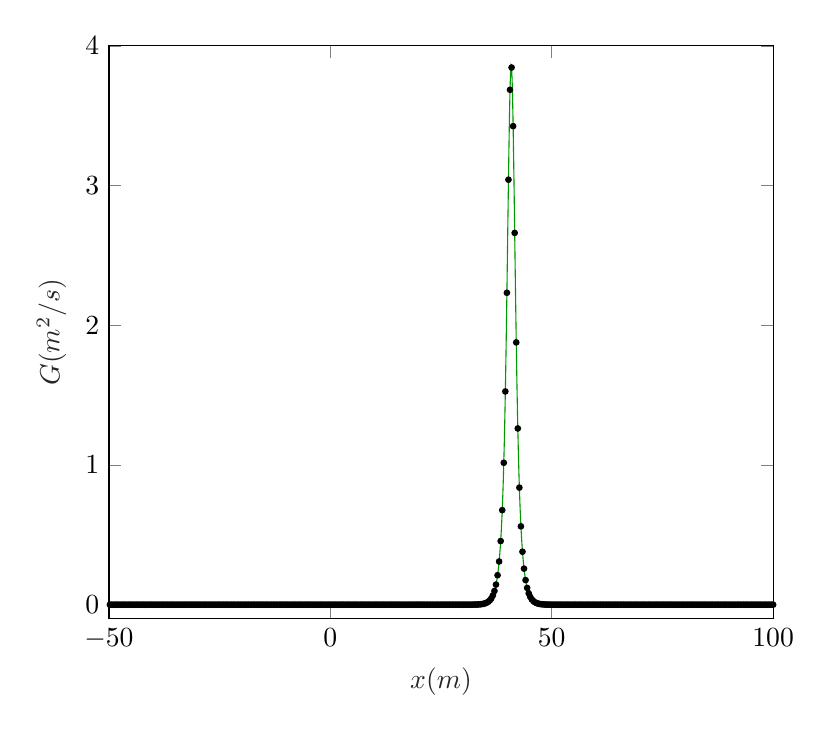
\begin{tikzpicture}

\begin{axis}[%
scale only axis,
xmin=-50,
xmax=100,
xtick={-50,   0,  50, 100},
xlabel style={font=\color{white!15!black}},
xlabel={$x (m)$},
ymin=-0.1,
ymax=4,
ytick={0, 1, 2, 3, 4},
ylabel style={font=\color{white!15!black}},
ylabel={$G (m^2/s)$},
axis background/.style={fill=white}
]
\addplot [color=green!60!black, forget plot]
  table[row sep=crcr]{%
-50.14064697609	-5.67925565028477e-44\\
-50.0234411626817	-6.46942449732437e-44\\
-49.9062353492733	-7.36953148507789e-44\\
-49.789029535865	-8.39487257823589e-44\\
-49.6718237224566	-9.56287190678446e-44\\
-49.5546179090483	-1.08933778628938e-43\\
-49.4374120956399	-1.2409000394494e-43\\
-49.3202062822316	-1.41354952273408e-43\\
-49.2030004688233	-1.61022015448423e-43\\
-49.0857946554149	-1.83425405633628e-43\\
-48.9685888420066	-2.08945834755365e-43\\
-48.8513830285982	-2.38016984129328e-43\\
-48.7341772151899	-2.71132874222405e-43\\
-48.6169714017815	-3.08856259787573e-43\\
-48.4997655883732	-3.51828193034678e-43\\
-48.3825597749648	-4.00778917348764e-43\\
-48.2653539615565	-4.56540276678192e-43\\
-48.1481481481481	-5.20059851471748e-43\\
-48.0309423347398	-5.92417061383291e-43\\
-47.9137365213315	-6.74841508385664e-43\\
-47.7965307079231	-7.68733872007089e-43\\
-47.6793248945148	-8.75689711773463e-43\\
-47.5621190811064	-9.97526581343133e-43\\
-47.4449132676981	-1.13631491509804e-42\\
-47.3277074542897	-1.29441321206272e-42\\
-47.2105016408814	-1.47450811504829e-42\\
-47.093295827473	-1.6796600661072e-42\\
-46.9760900140647	-1.91335531414344e-42\\
-46.8588842006564	-2.17956515847011e-42\\
-46.741678387248	-2.4828134350695e-42\\
-46.6244725738397	-2.82825339238234e-42\\
-46.5072667604313	-3.22175526301613e-42\\
-46.390060947023	-3.67000601952039e-42\\
-46.2728551336146	-4.18062300942952e-42\\
-46.1556493202063	-4.76228340062936e-42\\
-46.0384435067979	-5.42487163677648e-42\\
-45.9212376933896	-6.17964740855479e-42\\
-45.8040318799812	-7.03943699518549e-42\\
-45.6868260665729	-8.0188512277557e-42\\
-45.5696202531646	-9.13453377832024e-42\\
-45.4524144397562	-1.04054439940802e-41\\
-45.3352086263479	-1.18531790829781e-41\\
-45.2180028129395	-1.3502341125768e-41\\
-45.1007969995312	-1.53809551513841e-41\\
-44.9835911861228	-1.7520945380161e-41\\
-44.8663853727145	-1.99586777279541e-41\\
-44.7491795593061	-2.27355777901906e-41\\
-44.6319737458978	-2.58988348075698e-41\\
-44.5147679324894	-2.95022035762469e-41\\
-44.3975621190811	-3.36069179297554e-41\\
-44.2803563056728	-3.82827313159305e-41\\
-44.1631504922644	-4.36091021518543e-41\\
-44.0459446788561	-4.96765441001729e-41\\
-43.9287388654477	-5.65881642126743e-41\\
-43.8115330520394	-6.44614150795858e-41\\
-43.694327238631	-7.34300907597218e-41\\
-43.5771214252227	-8.36466004093106e-41\\
-43.4599156118143	-9.52845582464262e-41\\
-43.342709798406	-1.08541733863529e-40\\
-43.2255039849977	-1.23643413024305e-40\\
-43.1082981715893	-1.40846226056424e-40\\
-42.991092358181	-1.60442508898053e-40\\
-42.8738865447726	-1.827652709075e-40\\
-42.7566807313643	-2.081938538565e-40\\
-42.6394749179559	-2.3716037827318e-40\\
-42.5222691045476	-2.70157086680588e-40\\
-42.4050632911392	-3.07744708518192e-40\\
-42.2878574777309	-3.50561988895448e-40\\
-42.1706516643225	-3.99336543104426e-40\\
-42.0534458509142	-4.54897221347495e-40\\
-41.9362400375059	-5.18188193800127e-40\\
-41.8190342240975	-5.90284995363215e-40\\
-41.7018284106892	-6.72412802761265e-40\\
-41.5846225972808	-7.65967254578537e-40\\
-41.4674167838725	-8.72538168037957e-40\\
-41.3502109704641	-9.93936555554129e-40\\
-41.2330051570558	-1.13222540016589e-39\\
-41.1157993436474	-1.28975471283085e-39\\
-40.9985935302391	-1.46920146732771e-39\\
-40.8813877168308	-1.67361509139989e-39\\
-40.7641819034224	-1.90646928719458e-39\\
-40.6469760900141	-2.17172106160686e-39\\
-40.5297702766057	-2.47387796966146e-39\\
-40.4125644631974	-2.81807471363196e-39\\
-40.295358649789	-3.21016039958451e-39\\
-40.1781528363807	-3.65679793413976e-39\\
-40.0609470229723	-4.16557725055085e-39\\
-39.943741209564	-4.74514428820606e-39\\
-39.8265353961556	-5.40534791736657e-39\\
-39.7093295827473	-6.1574073059063e-39\\
-39.592123769339	-7.01410257219832e-39\\
-39.4749179559306	-7.98999196400849e-39\\
-39.3577121425223	-9.10165925402394e-39\\
-39.2405063291139	-1.03679955561304e-38\\
-39.1233005157056	-1.1810520351486e-38\\
-39.0060947022972	-1.3453747179742e-38\\
-38.8888888888889	-1.53256002097858e-38\\
-38.7716830754805	-1.74578887690003e-38\\
-38.6544772620722	-1.98868478949472e-38\\
-38.5372714486639	-2.26537540953428e-38\\
-38.4200656352555	-2.58056267802317e-38\\
-38.3028598218472	-2.93960272861585e-38\\
-38.1856540084388	-3.34859690705341e-38\\
-38.0684481950305	-3.81449545435936e-38\\
-37.9512423816221	-4.34521561573435e-38\\
-37.8340365682138	-4.94977618223231e-38\\
-37.7168307548054	-5.63845075155249e-38\\
-37.5996249413971	-6.42294231238227e-38\\
-37.4824191279887	-7.31658211909224e-38\\
-37.3652133145804	-8.3345562363561e-38\\
-37.2480075011721	-9.49416360348316e-38\\
-37.1308016877637	-1.08151100038787e-37\\
-37.0135958743554	-1.2319842935199e-37\\
-36.896390060947	-1.40339330708186e-37\\
-36.7791842475387	-1.59865087949707e-37\\
-36.6619784341303	-1.82107511958348e-37\\
-36.544772620722	-2.07444579282335e-37\\
-36.4275668073136	-2.36306855279352e-37\\
-36.3103609939053	-2.69184810927339e-37\\
-36.193155180497	-3.06637157641179e-37\\
-36.0759493670886	-3.49300341733039e-37\\
-35.9587435536803	-3.97899359860334e-37\\
-35.8415377402719	-4.53260079253712e-37\\
-35.7243319268636	-5.16323272088679e-37\\
-35.6071261134552	-5.88160602494042e-37\\
-35.4899203000469	-6.699928378722e-37\\
-35.3727144866385	-7.63210594005375e-37\\
-35.2555086732302	-8.69397966479689e-37\\
-35.1383028598218	-9.90359450007444e-37\\
-35.0210970464135	-1.12815060310125e-36\\
-34.9038912330052	-1.28511297919975e-36\\
-34.7866854195968	-1.46391391784721e-36\\
-34.6694796061885	-1.66759187211797e-36\\
-34.5522737927801	-1.89960804255711e-36\\
-34.4350679793718	-2.16390519507907e-36\\
-34.3178621659634	-2.46497466234507e-36\\
-34.2006563525551	-2.80793266720784e-36\\
-34.0834505391467	-3.19860726522513e-36\\
-33.9662447257384	-3.64363738370003e-36\\
-33.8490389123301	-4.15058564026676e-36\\
-33.7318330989217	-4.72806685820487e-36\\
-33.6146272855134	-5.38589446240624e-36\\
-33.497421472105	-6.13524724377348e-36\\
-33.3802156586967	-6.98885932596121e-36\\
-33.2630098452883	-7.96123656265768e-36\\
-33.14580403188	-9.06890304275518e-36\\
-33.0285982184716	-1.03306818923917e-35\\
-32.9113924050633	-1.17680151456735e-35\\
-32.7941865916549	-1.34053281198016e-35\\
-32.6769807782466	-1.52704444866057e-35\\
-32.5597749648383	-1.73950590940077e-35\\
-32.4425691514299	-1.98152765722979e-35\\
-32.3253633380216	-2.25722248780352e-35\\
-32.2081575246132	-2.57127542018214e-35\\
-32.0909517112049	-2.92902331168347e-35\\
-31.9737458977965	-3.33654554974806e-35\\
-31.8565400843882	-3.80076736198637e-35\\
-31.7393342709798	-4.32957750000788e-35\\
-31.6221284575715	-4.93196229689201e-35\\
-31.5049226441632	-5.61815837640502e-35\\
-31.3877168307548	-6.39982660902768e-35\\
-31.2705110173465	-7.29025027091278e-35\\
-31.1533052039381	-8.30456077318933e-35\\
-31.0360993905298	-9.45999479753952e-35\\
-30.9188935771214	-1.07761872076836e-34\\
-30.8016877637131	-1.22755047143627e-34\\
-30.6844819503047	-1.39834259639528e-34\\
-30.5672761368964	-1.59289745097464e-34\\
-30.450070323488	-1.81452120235933e-34\\
-30.3328645100797	-2.06698001292991e-34\\
-30.2156586966714	-2.3545640405285e-34\\
-30.098452883263	-2.68216034323976e-34\\
-29.9812470698547	-3.05533592759417e-34\\
-29.8640412564463	-3.48043235147226e-34\\
-29.746835443038	-3.96467348934472e-34\\
-29.6296296296296	-4.51628829115533e-34\\
-29.5124238162213	-5.14465062095144e-34\\
-29.3952180028129	-5.86043855160665e-34\\
-29.2780121894046	-6.67581582261175e-34\\
-29.1608063759962	-7.60463854453612e-34\\
-29.0436005625879	-8.66269066278986e-34\\
-28.9263947491796	-9.86795218204107e-34\\
-28.8091889357712	-1.12409047093557e-33\\
-28.6919831223629	-1.28048795083117e-33\\
-28.5747773089545	-1.45864539787368e-33\\
-28.4575714955462	-1.6615903299652e-33\\
-28.3403656821378	-1.89277149104129e-33\\
-28.2231598687295	-2.15611745728783e-33\\
-28.1059540553211	-2.45610339738575e-33\\
-27.9887482419128	-2.79782712127288e-33\\
-27.8715424285045	-3.18709570975801e-33\\
-27.7543366150961	-3.63052419712644e-33\\
-27.6371308016878	-4.13564798370029e-33\\
-27.5199249882794	-4.71105088863525e-33\\
-27.4027191748711	-5.36651101901884e-33\\
-27.2855133614627	-6.11316693409651e-33\\
-27.1683075480544	-6.96370692833562e-33\\
-27.051101734646	-7.93258464990982e-33\\
-26.9338959212377	-9.03626471871409e-33\\
-26.8166901078293	-1.02935025178213e-32\\
-26.699484294421	-1.17256629130129e-32\\
-26.5822784810127	-1.33570833165449e-32\\
-26.4650726676043	-1.52154872648717e-32\\
-26.347866854196	-1.73324555384564e-32\\
-26.2306610407876	-1.97439628296455e-32\\
-26.1134552273793	-2.24909890784659e-32\\
-25.9962494139709	-2.5620215865082e-32\\
-25.8790436005626	-2.91848196930506e-32\\
-25.7618377871542	-3.32453756440329e-32\\
-25.6446319737459	-3.78708867602171e-32\\
-25.5274261603376	-4.3139956647252e-32\\
-25.4102203469292	-4.91421252243247e-32\\
-25.2930145335209	-5.59793903204352e-32\\
-25.1758087201125	-6.37679409741217e-32\\
-25.0586029067042	-7.26401318914445e-32\\
-24.9413970932958	-8.27467326151825e-32\\
-24.8241912798875	-9.42594896264916e-32\\
-24.7069854664791	-1.07374044918077e-31\\
-24.5897796530708	-1.22313260635659e-31\\
-24.4725738396624	-1.39331006285001e-31\\
-24.3553680262541	-1.58716472862398e-31\\
-24.2381622128458	-1.80799087220775e-31\\
-24.1209563994374	-2.05954110183665e-31\\
-24.0037505860291	-2.34609013538603e-31\\
-23.8865447726207	-2.67250744277318e-31\\
-23.7693389592124	-3.04433999527589e-31\\
-23.652133145804	-3.46790652796809e-31\\
-23.5349273323957	-3.95040491712024e-31\\
-23.4177215189873	-4.50003449728256e-31\\
-23.300515705579	-5.12613539664557e-31\\
-23.1833098921707	-5.83934725847349e-31\\
-23.0661040787623	-6.65179004584142e-31\\
-22.948898265354	-7.5772700021819e-31\\
-22.8316924519456	-8.63151426763096e-31\\
-22.7144866385373	-9.83243813812407e-31\\
-22.5972808251289	-1.120044950891e-30\\
-22.4800750117206	-1.27587956760414e-30\\
-22.3628691983122	-1.45339583892122e-30\\
-22.2456633849039	-1.65561038692719e-30\\
-22.1284575714955	-1.88595954377831e-30\\
-22.0112517580872	-2.14835774699988e-30\\
-21.8940459446789	-2.44726405946538e-30\\
-21.7768401312705	-2.7877579444646e-30\\
-21.6596343178622	-3.17562558354374e-30\\
-21.5424285044538	-3.61745820395983e-30\\
-21.4252226910455	-4.12076408667597e-30\\
-21.3080168776371	-4.69409615830541e-30\\
-21.1908110642288	-5.34719733523786e-30\\
-21.0736052508204	-6.09116608985208e-30\\
-20.9563994374121	-6.93864505236433e-30\\
-20.8391936240038	-7.90403585331695e-30\\
-20.7219878105954	-9.0037438576331e-30\\
-20.6047819971871	-1.02564569491223e-29\\
-20.4875761837787	-1.16834631029645e-29\\
-20.3703703703704	-1.33090121428349e-29\\
-20.253164556962	-1.51607278301914e-29\\
-20.1359587435537	-1.72700772885597e-29\\
-20.0187529301453	-1.96729057399784e-29\\
-19.901547116737	-2.24100456406447e-29\\
-19.7843413033286	-2.55280105671022e-29\\
-19.6671354899203	-2.90797856445299e-29\\
-19.549929676512	-3.31257279492657e-29\\
-19.4327238631036	-3.77345921865547e-29\\
-19.3155180496953	-4.29846990733726e-29\\
-19.1983122362869	-4.89652662812327e-29\\
-19.0811064228786	-5.57779245563524e-29\\
-18.9639006094702	-6.35384447813479e-29\\
-18.8466947960619	-7.23787053272964e-29\\
-18.7294889826535	-8.24489331283325e-29\\
-18.6122831692452	-9.39202565624859e-29\\
-18.4950773558368	-1.06987613521126e-28\\
-18.3778715424285	-1.21873064085278e-28\\
-18.2606657290202	-1.38829564102781e-28\\
-18.1434599156118	-1.58145263792512e-28\\
-18.0262541022035	-1.80148404424055e-28\\
-17.9090482887951	-2.0521289628447e-28\\
-17.7918424753868	-2.3376467272134e-28\\
-17.6746366619784	-2.66288928239499e-28\\
-17.5574308485701	-3.03338363652019e-28\\
-17.4402250351617	-3.45542578399383e-28\\
-17.3230192217534	-3.93618769645192e-28\\
-17.2058134083451	-4.48383919963454e-28\\
-17.0886075949367	-5.10768680728865e-28\\
-16.9714017815284	-5.81833187137416e-28\\
-16.85419596812	-6.62785073609845e-28\\
-16.7369901547117	-7.54999995722585e-28\\
-16.6197843413033	-8.60045007405599e-28\\
-16.502578527895	-9.79705190667434e-28\\
-16.3853727144866	-1.11601399037952e-27\\
-16.2681669010783	-1.27128776961395e-27\\
-16.1509610876699	-1.44816517275059e-27\\
-16.0337552742616	-1.64965196527029e-27\\
-15.9165494608533	-1.87917211221926e-27\\
-15.7993436474449	-2.14062596334618e-27\\
-15.6821378340366	-2.4384565336808e-27\\
-15.5649320206282	-2.77772500589302e-27\\
-15.4477262072199	-3.16419673748154e-27\\
-15.3305203938115	-3.6044392343547e-27\\
-15.2133145804032	-4.10593375571712e-27\\
-15.0961087669948	-4.67720244681982e-27\\
-14.9789029535865	-5.32795316000339e-27\\
-14.8616971401782	-6.06924442504969e-27\\
-14.7444913267698	-6.91367337226614e-27\\
-14.6272855133615	-7.87558980177177e-27\\
-14.5100796999531	-8.97134003677153e-27\\
-14.3928738865448	-1.02195447047372e-26\\
-14.2756680731364	-1.16414151669705e-26\\
-14.1584622597281	-1.3261113973791e-26\\
-14.0412564463197	-1.51061654707431e-26\\
-13.9240506329114	-1.72079235334581e-26\\
-13.806844819503	-1.96021043796217e-26\\
-13.6896390060947	-2.23293935123833e-26\\
-13.5724331926864	-2.54361371092997e-26\\
-13.455227379278	-2.89751296059287e-26\\
-13.3380215658697	-3.30065108578702e-26\\
-13.2208157524613	-3.75987881271732e-26\\
-13.103609939053	-4.28300002602356e-26\\
-12.9864041256446	-4.87890438406459e-26\\
-12.8691983122363	-5.55771838529369e-26\\
-12.7519924988279	-6.33097745287205e-26\\
-12.6347866854196	-7.21182196183838e-26\\
-12.5175808720113	-8.21522054002271e-26\\
-12.4003750586029	-9.35822443736625e-26\\
-12.2831692451946	-1.06602572862732e-25\\
-12.1659634317862	-1.21434451770346e-25\\
-12.0487576183779	-1.38329926574592e-25\\
-11.9315518049695	-1.57576110462623e-25\\
-11.8143459915612	-1.79500063387508e-25\\
-11.6971401781528	-2.04474349960316e-25\\
-11.5799343647445	-2.32923370625412e-25\\
-11.4627285513361	-2.65330573707812e-25\\
-11.3455227379278	-3.0224667089047e-25\\
-11.2283169245195	-3.44298995731157e-25\\
-11.1111111111111	-3.9220216425292e-25\\
-10.9939052977028	-4.46770218768769e-25\\
-10.8766994842944	-5.08930461306618e-25\\
-10.7594936708861	-5.79739211712812e-25\\
-10.6422878574777	-6.60399758219424e-25\\
-10.5250820440694	-7.52282805518297e-25\\
-10.407876230661	-8.56949767825991e-25\\
-10.2906704172527	-9.76179302770403e-25\\
-10.1734646038444	-1.11199753700245e-24\\
-10.056258790436	-1.26671249717158e-24\\
-9.93905297702766	-1.44295333136797e-24\\
-9.82184716361932	-1.64371498754059e-24\\
-9.70464135021097	-1.87240910813395e-24\\
-9.58743553680262	-2.1329220058209e-24\\
-9.47022972339428	-2.42968070554245e-24\\
-9.35302390998594	-2.7677281751394e-24\\
-9.23581809657759	-3.15280902300708e-24\\
-9.11861228316924	-3.59146711907652e-24\\
-9.0014064697609	-4.09115679804335e-24\\
-8.88420065635255	-4.66036953457618e-24\\
-8.76699484294421	-5.30877824315931e-24\\
-8.64978902953587	-6.04740165472831e-24\\
-8.53258321612752	-6.88879156343276e-24\\
-8.41537740271917	-7.84724612550216e-24\\
-8.29817158931083	-8.93905283491006e-24\\
-8.18096577590249	-1.01827653048414e-23\\
-8.06375996249414	-1.15995185584475e-23\\
-7.94655414908579	-1.32133881867822e-23\\
-7.82934833567745	-1.50517994772675e-23\\
-7.7121425222691	-1.71459934652117e-23\\
-7.59493670886076	-1.95315578282238e-23\\
-7.47773089545242	-2.22490316452794e-23\\
-7.36052508204407	-2.53445942974058e-23\\
-7.24331926863572	-2.88708502168173e-23\\
-7.12611345522738	-3.28877228201366e-23\\
-7.00890764181904	-3.7463472816748e-23\\
-6.89170182841069	-4.26758581969034e-23\\
-6.77449601500234	-4.8613455611836e-23\\
-6.657290201594	-5.53771656007476e-23\\
-6.54008438818565	-6.30819272437408e-23\\
-6.42287857477731	-7.18586713786387e-23\\
-6.30567276136896	-8.18565455736856e-23\\
-6.18846694796062	-9.32454486661817e-23\\
-6.07126113455227	-1.06218917937732e-22\\
-5.95405532114393	-1.20997417989309e-22\\
-5.83684950773559	-1.37832087205614e-22\\
-5.71964369432724	-1.57009005474272e-22\\
-5.60243788091889	-1.78854055683312e-22\\
-5.48523206751055	-2.03738461610793e-22\\
-5.3680262541022	-2.32085096314685e-22\\
-5.25082044069386	-2.64375668224554e-22\\
-5.13361462728551	-3.0115890705196e-22\\
-5.01640881387717	-3.43059888626723e-22\\
-4.89920300046882	-3.90790657120676e-22\\
-4.78199718706048	-4.45162325167598e-22\\
-4.66479137365214	-5.07098857502693e-22\\
-4.54758556024379	-5.77652772353829e-22\\
-4.43037974683544	-6.58023027406032e-22\\
-4.31317393342709	-7.49575394284404e-22\\
-4.19596812001875	-8.53865667789042e-22\\
-4.07876230661041	-9.726661042881e-22\\
-3.96155649320206	-1.10799553854966e-21\\
-3.84435067979372	-1.26215369080274e-21\\
-3.72714486638537	-1.43776024702432e-21\\
-3.60993905297703	-1.637799376563e-21\\
-3.49273323956868	-1.86567044360962e-21\\
-3.37552742616034	-2.12524577427976e-21\\
-3.25832161275199	-2.42093646097287e-21\\
-3.14111579934364	-2.75776732225433e-21\\
-3.0239099859353	-3.14146229209073e-21\\
-2.90670417252696	-3.57854168950001e-21\\
-2.78949835911861	-4.07643302156808e-21\\
-2.67229254571027	-4.6435972027623e-21\\
-2.55508673230192	-5.28967233544967e-21\\
-2.43788091889358	-6.02563749495257e-21\\
-2.32067510548523	-6.86399930242403e-21\\
-2.20346929207689	-7.81900445606685e-21\\
-2.08626347866854	-8.90688183234557e-21\\
-1.96905766526019	-1.01461182713373e-20\\
-1.85185185185185	-1.15577727327786e-20\\
-1.73464603844351	-1.3165834161418e-20\\
-1.61744022503516	-1.4997629143058e-20\\
-1.50023441162681	-1.70842862787873e-20\\
-1.38302859821847	-1.94612651687457e-20\\
-1.26582278481013	-2.21689589947048e-20\\
-1.14861697140178	-2.52533809414499e-20\\
-1.03141115799344	-2.87669461216609e-20\\
-0.914205344585092	-3.2769362291932e-20\\
-0.796999531176745	-3.73286444963069e-20\\
-0.679793717768398	-4.2522270879673e-20\\
-0.562587904360058	-4.84384993123216e-20\\
-0.445382090951711	-5.51778671997359e-20\\
-0.328176277543363	-6.28548999646078e-20\\
-0.210970464135023	-7.16000572341759e-20\\
-0.0937646507266763	-8.15619498054077e-20\\
0.0234411626816708	-9.29098650620153e-20\\
0.140646976090011	-1.05836643758969e-19\\
0.257852789498358	-1.2056195706114e-19\\
0.375058602906705	-1.37336039524405e-19\\
0.492264416315052	-1.56443941455628e-19\\
0.609470229723392	-1.7821037291397e-19\\
0.726676043131739	-2.03005221670051e-19\\
0.843881856540087	-2.3124983889238e-19\\
0.961087669948427	-2.63424199376843e-19\\
1.07829348335677	-3.0007505799658e-19\\
1.19549929676512	-3.41825240978853e-19\\
1.31270511017347	-3.89384229900186e-19\\
1.42991092358181	-4.43560218258835e-19\\
1.54711673699016	-5.0527384550797e-19\\
1.6643225503985	-5.75573841938713e-19\\
1.78152836380684	-6.55654850274386e-19\\
1.89873417721519	-7.468777268271e-19\\
2.01593999062354	-8.50792667204355e-19\\
2.13314580403188	-9.69165549552229e-19\\
2.25035161744022	-1.10400794299894e-18\\
2.36755743084857	-1.25761129124728e-18\\
2.48476324425692	-1.43258585221445e-18\\
2.60196905766526	-1.63190505544009e-18\\
2.71917487107361	-1.85895603104999e-18\\
2.83638068448195	-2.11759716893897e-18\\
2.95358649789029	-2.41222368630501e-18\\
3.07079231129864	-2.74784231775607e-18\\
3.18799812470699	-3.13015639723567e-18\\
3.30520393811533	-3.56566277760675e-18\\
3.42240975152367	-4.06176223489603e-18\\
3.53961556493202	-4.62688523335374e-18\\
3.65682137834037	-5.27063518851562e-18\\
3.77402719174871	-6.00395166280868e-18\\
3.89123300515705	-6.83929626696383e-18\\
4.0084388185654	-7.79086442635072e-18\\
4.12564463197375	-8.87482661088508e-18\\
4.24285044538209	-1.01096031278477e-17\\
4.36005625879044	-1.15161771473073e-17\\
4.47726207219878	-1.31184512795408e-17\\
4.59446788560712	-1.49436537639508e-17\\
4.71167369901547	-1.70228011720496e-17\\
4.82887951242382	-1.93912254874488e-17\\
4.94608532583216	-2.20891745197898e-17\\
5.0632911392405	-2.51624958557439e-17\\
5.18049695264885	-2.86634159698041e-17\\
5.2977027660572	-3.26514277346808e-17\\
5.41490857946554	-3.71943014132084e-17\\
5.53211439287389	-4.23692363120529e-17\\
5.64932020628223	-4.82641726678348e-17\\
5.76652601969058	-5.49792860592091e-17\\
5.88373183309892	-6.262868974018e-17\\
6.00093764650727	-7.13423738232549e-17\\
6.11814345991561	-8.12684142659256e-17\\
6.23534927332395	-9.25754891988914e-17\\
6.3525550867323	-1.0545574535724e-16\\
6.46976090014065	-1.20128063325257e-16\\
6.58696671354899	-1.36841777082808e-16\\
6.70417252695734	-1.55880911061387e-16\\
6.82137834036568	-1.77569006712211e-16\\
6.93858415377403	7.04499652447659e-16\\
7.05578996718237	6.76356685553378e-16\\
7.17299578059072	6.44298118257833e-16\\
7.29020159399906	6.07779163419e-16\\
7.4074074074074	5.66179236316026e-16\\
7.52461322081575	5.187914087451e-16\\
7.6418190342241	4.6481039583772e-16\\
7.75902484763245	4.03318871455313e-16\\
7.87623066104079	1.2400461526653e-15\\
7.99343647444913	1.16025335006822e-15\\
8.11064228785748	1.06935877802938e-15\\
8.22784810126582	9.6581781998282e-16\\
8.34505391467417	1.75464522610409e-15\\
8.46225972808251	1.62028812064766e-15\\
8.57946554149086	1.46723757970471e-15\\
8.6966713548992	2.19966701254122e-15\\
8.81387716830755	2.00106514466603e-15\\
8.9310829817159	2.68160558209758e-15\\
9.04828879512424	3.33066954795203e-15\\
9.16549460853258	3.03710337004486e-15\\
9.28270042194093	3.60946687875131e-15\\
9.39990623534927	4.13530299295864e-15\\
9.51711204875762	5.51491251456027e-15\\
9.63431786216596	5.92737275627671e-15\\
9.75152367557431	6.27105786754127e-15\\
9.86872948898265	7.4431732678683e-15\\
9.985935302391	8.52604449246784e-15\\
10.1031411157993	9.50725477904178e-15\\
10.2203469292077	1.12794340635809e-14\\
10.337552742616	1.2919695799463e-14\\
10.4547585560244	1.44096859727564e-14\\
10.5719643694327	1.66352712033538e-14\\
10.6891701828411	1.8665860631684e-14\\
10.8063759962494	2.13810982838562e-14\\
10.9235818096578	2.38433049416946e-14\\
11.0407876230661	2.78308243249419e-14\\
11.1579934364744	3.14900049267945e-14\\
11.2751992498828	3.56819384357729e-14\\
11.3924050632911	4.03545863366771e-14\\
11.5096108766995	4.63554441403836e-14\\
11.6268166901078	5.27102112112611e-14\\
11.7440225035162	6.02487403504022e-14\\
11.8612283169245	6.88834078117178e-14\\
11.9784341303329	7.85143985411919e-14\\
12.0956399437412	8.90280099701405e-14\\
12.2128457571496	1.01201494084096e-13\\
12.3300515705579	1.15794082113248e-13\\
12.4472573839662	1.31730928714194e-13\\
12.5644631973746	1.49727352947061e-13\\
12.6816690107829	1.71378810509016e-13\\
12.7988748241913	1.94623316208983e-13\\
12.9160806375996	2.21898190617956e-13\\
13.033286451008	2.52881056686928e-13\\
13.1504922644163	2.88111458525937e-13\\
13.2676980778247	3.28077846606643e-13\\
13.384903891233	3.73210468978376e-13\\
13.5021097046413	4.2568682196768e-13\\
13.6193155180497	4.84888554293072e-13\\
13.736521331458	5.51924830480177e-13\\
13.8537271448664	6.28713586641477e-13\\
13.9709329582747	7.17061120847776e-13\\
14.0881387716831	8.15926237832966e-13\\
14.2053445850914	9.29563523903678e-13\\
14.3225503984998	1.05934222318704e-12\\
14.4397562119081	1.20644360089922e-12\\
14.5569620253165	1.37455511219495e-12\\
14.6741678387248	1.56621351223959e-12\\
14.7913736521331	1.78367769249551e-12\\
14.9085794655415	2.0316103436789e-12\\
15.0257852789498	2.31431359423626e-12\\
15.1429910923582	2.63658561869945e-12\\
15.2601969057665	3.00366349205996e-12\\
15.3774027191749	3.42115809333096e-12\\
15.4946085325832	3.89770027490109e-12\\
15.6118143459916	4.43941574627565e-12\\
15.7290201593999	5.05708304503515e-12\\
15.8462259728083	5.76058328019619e-12\\
15.9634317862166	6.56240236785392e-12\\
16.0806375996249	7.47567524890499e-12\\
16.1978434130333	8.51583741453226e-12\\
16.3150492264416	9.70044034047623e-12\\
16.43225503985	1.10498480164934e-11\\
16.5494608532583	1.25869974496629e-11\\
16.6666666666667	1.43389393944725e-11\\
16.783872480075	1.63338072536351e-11\\
16.9010782934834	1.86059037082805e-11\\
17.0182841068917	2.11943906731916e-11\\
17.1354899203	2.41437366925726e-11\\
17.2526957337084	2.75022868728026e-11\\
17.3699015471167	3.13289209766071e-11\\
17.4871073605251	3.56878405148137e-11\\
17.6043131739334	4.06532358790363e-11\\
17.7215189873418	4.63093119822287e-11\\
17.8387248007501	5.27529116277478e-11\\
17.9559306141585	6.00923721301736e-11\\
18.0731364275668	6.84534770491427e-11\\
18.1903422409752	7.79779725144793e-11\\
18.3075480543835	8.88264109953478e-11\\
18.4247538677918	1.01185293792682e-10\\
18.5419596812002	1.15263971149788e-10\\
18.6591654946085	1.31300304972158e-10\\
18.7763713080169	1.49568704282621e-10\\
18.8935771214252	1.70378696985551e-10\\
19.0107829348336	1.94083931884914e-10\\
19.1279887482419	2.21087039813816e-10\\
19.2451945616503	2.51847536584693e-10\\
19.3624003750586	2.86887245683508e-10\\
19.4796061884669	3.26803122464384e-10\\
19.5968120018753	3.72271959015278e-10\\
19.7140178152836	4.2406679836046e-10\\
19.831223628692	4.8306859894736e-10\\
19.9484294421003	5.50279340645031e-10\\
20.0656352555087	6.2684092820148e-10\\
20.182841068917	7.14054248834957e-10\\
20.3000468823254	8.134026869523e-10\\
20.4172526957337	9.26573485573149e-10\\
20.5344585091421	1.05548934970686e-09\\
20.6516643225504	1.20234269621174e-09\\
20.7688701359587	1.36962762750629e-09\\
20.8860759493671	1.56018732177038e-09\\
21.0032817627754	1.77726001323682e-09\\
21.1204875761838	2.02453477599012e-09\\
21.2376933895921	2.30621282957294e-09\\
21.3548992030005	2.62708178169132e-09\\
21.4721050164088	2.99259470439821e-09\\
21.5893108298172	3.40896123711507e-09\\
21.7065166432255	3.88325868200008e-09\\
21.8237224566338	4.42354642090899e-09\\
21.9409282700422	5.039004893022e-09\\
22.0581340834505	5.74009387675532e-09\\
22.1753398968589	6.53872731321492e-09\\
22.2925457102672	7.44847706538602e-09\\
22.4097515236756	8.48480229793672e-09\\
22.5269573370839	9.66531352227517e-09\\
22.6441631504923	1.10100718088318e-08\\
22.7613689639006	1.25419304879271e-08\\
22.878574777309	1.42869207246381e-08\\
22.9957805907173	1.62746953904763e-08\\
23.1129864041256	1.85390327705267e-08\\
23.230192217534	2.11184149675598e-08\\
23.3473980309423	2.40566719078874e-08\\
23.4646038443507	2.74037357635419e-08\\
23.581809657759	3.12164851421731e-08\\
23.6990154711674	3.55597115697239e-08\\
23.8162212845757	4.05072217045498e-08\\
23.9334270979841	4.61430921092188e-08\\
24.0506329113924	5.25630938509119e-08\\
24.1678387248007	5.98763261550833e-08\\
24.2850445382091	6.82070678624435e-08\\
24.4022503516174	7.76968853896477e-08\\
24.5194561650258	8.85070437070075e-08\\
24.6366619784341	1.00821247029413e-07\\
24.7538677918425	1.1484875460448e-07\\
24.8710736052508	1.30827945090361e-07\\
24.9882794186592	1.49030359311305e-07\\
25.1054852320675	1.69765320102649e-07\\
25.2226910454759	1.93385186342083e-07\\
25.3398968588842	2.20291342766761e-07\\
25.4571026722925	2.50941018476639e-07\\
25.5743084857009	2.85855058826503e-07\\
25.6915142991092	3.25626774548931e-07\\
25.8087201125176	3.70932027150908e-07\\
25.9259259259259	4.22540709487775e-07\\
26.0431317393343	4.81329833101205e-07\\
26.1603375527426	5.4829843077014e-07\\
26.277543366151	6.24584532254987e-07\\
26.3947491795593	7.1148450277315e-07\\
26.5119549929676	8.10475075926028e-07\\
26.629160806376	9.23238446084501e-07\\
26.7463666197843	1.05169085352027e-06\\
26.8635724331927	1.19801515152588e-06\\
26.980778246601	1.3646978958533e-06\\
27.0979840600094	1.55457160478368e-06\\
27.2151898734177	1.77086288830396e-06\\
27.3323956868261	2.01724728352007e-06\\
27.4496015002344	2.29791170841468e-06\\
27.5668073136428	2.61762561877808e-06\\
27.6840131270511	2.98182205022739e-06\\
27.8012189404594	3.39668994642382e-06\\
27.9184247538678	3.86927932937337e-06\\
28.0356305672761	4.40762109996003e-06\\
28.1528363806845	5.02086350780401e-06\\
28.2700421940928	5.71942760981789e-06\\
28.3872480075012	6.51518435488633e-06\\
28.5044538209095	7.42165630450217e-06\\
28.6216596343179	8.454247420254e-06\\
28.7388654477262	9.63050481972133e-06\\
28.8560712611346	1.09704169509731e-05\\
28.9732770745429	1.24967532438382e-05\\
29.0904828879512	1.42354510177999e-05\\
29.2076887013596	1.62160562181099e-05\\
29.3248945147679	1.84722254612266e-05\\
29.4421003281763	2.10422979253289e-05\\
29.5593061415846	2.39699467943057e-05\\
29.676511954993	2.73049213320218e-05\\
29.7937177684013	3.11038921735575e-05\\
29.9109235818097	3.543141420647e-05\\
30.028129395218	4.03610233869567e-05\\
30.1453352086263	4.59764861124935e-05\\
30.2625410220347	5.23732223738739e-05\\
30.379746835443	5.96599268373539e-05\\
30.4969526488514	6.79604153903211e-05\\
30.6141584622597	7.74157284720337e-05\\
30.7313642756681	8.81865268958671e-05\\
30.8485700890764	0.000100455820813016\\
30.9657759024848	0.000114432078097946\\
31.0829817158931	0.000130352764879346\\
31.2001875293015	0.000148488378236566\\
31.3173933427098	0.000169147039410214\\
31.4345991561181	0.000192679725343126\\
31.5518049695265	0.000219486227146894\\
31.6690107829348	0.000250021936355717\\
31.7862165963432	0.000284805573764508\\
31.9034224097515	0.000324427991524394\\
32.0206282231599	0.00036956219721324\\
32.1378340365682	0.00042097476908627\\
32.2550398499766	0.000479538855050475\\
32.3722456633849	0.000546248974354167\\
32.4894514767932	0.000622237871096495\\
32.6066572902016	0.000708795702770705\\
32.7238631036099	0.000807391885842149\\
32.8410689170183	0.000919699964270065\\
32.9582747304266	0.00104762591672266\\
33.075480543835	0.00119334037464924\\
33.1926863572433	0.00135931528724505\\
33.3098921706517	0.00154836564156118\\
33.42709798406	0.00176369692761302\\
33.5443037974684	0.00200895913045486\\
33.6615096108767	0.00228830813496124\\
33.778715424285	0.0026064755459206\\
33.8959212376934	0.00296884805739681\\
34.0131270511017	0.00338155765261079\\
34.1303328645101	0.0038515840807093\\
34.2475386779184	0.0043868712411525\\
34.3647444913268	0.00499645931221381\\
34.4819503047351	0.00569063468894814\\
34.5991561181435	0.00648110004999354\\
34.7163619315518	0.00738116715395361\\
34.8335677449601	0.00840597527687077\\
34.9507735583685	0.00957273854516631\\
35.0679793717768	0.0109010257960637\\
35.1851851851852	0.0124130770137129\\
35.3023909985935	0.0141341608487715\\
35.4195968120019	0.0160929782392172\\
35.5368026254102	0.0183221177212166\\
35.6540084388186	0.0208585686674843\\
35.7712142522269	0.0237442994420471\\
35.8884200656353	0.0270269083544166\\
36.0056258790436	0.0307603563934693\\
36.122831692452	0.035005792114396\\
36.2400375058603	0.0398324808794348\\
36.3572433192686	0.0453188531192728\\
36.474449132677	0.0515536896839815\\
36.5916549460853	0.058637467113298\\
36.7088607594937	0.0666838923661058\\
36.826066572902	0.0758216660114743\\
36.9432723863104	0.0861965261589085\\
37.0604781997187	0.0979736438396166\\
37.177684013127	0.111340465761539\\
37.2948898265354	0.126510134136342\\
37.4120956399437	0.143725657307186\\
37.5293014533521	0.163265060239153\\
37.6465072667604	0.18544780997582\\
37.7637130801688	0.210642884009107\\
37.8809188935771	0.239278919318419\\
37.9981247069855	0.271856927019288\\
38.1153305203938	0.308966047623336\\
38.2325363338022	0.351302699209388\\
38.3497421472105	0.399693152289034\\
38.4669479606189	0.455118936508369\\
38.5841537740272	0.518743403174827\\
38.7013595874355	0.591936081115553\\
38.8185654008439	0.676289050626706\\
38.9357712142522	0.773616410414419\\
39.0529770276606	0.885924245950563\\
39.1701828410689	1.01533493398509\\
39.2873886544773	1.16394729396258\\
39.4045944678856	1.33361480679152\\
39.5218002812939	1.5256301458044\\
39.6390060947023	1.74031788213731\\
39.7562119081106	1.97655972760745\\
39.873417721519	2.23130695402441\\
39.9906235349273	2.4991677259524\\
40.1078293483357	2.7721835271631\\
40.225035161744	3.03991577737864\\
40.3422409751524	3.28993855737342\\
40.4594467885607	3.5087697683505\\
40.5766526019691	3.6831771393487\\
40.6938584153774	3.80168867345452\\
40.8110642287858	3.85605242448379\\
40.9282700421941	3.84236156950501\\
41.0454758556024	3.76160713576826\\
41.1626816690108	3.61953661767913\\
41.2798874824191	3.42584992208795\\
41.3970932958275	3.1929075462474\\
41.5142991092358	2.93421649157851\\
41.6315049226442	2.66297480376634\\
41.7487107360525	2.39090093158618\\
41.8659165494608	2.12747622706502\\
41.9831223628692	1.87962296362839\\
42.1003281762775	1.65175555341958\\
42.2175339896859	1.44609450039702\\
42.3347398030942	1.2631215430121\\
42.4519456165026	1.10207080682944\\
42.5691514299109	0.961381300553836\\
42.6863572433193	0.83906894293178\\
42.8035630567276	0.733003824786157\\
42.920768870136	0.641097321765158\\
43.0379746835443	0.56141401545166\\
43.1551804969527	0.492226988879258\\
43.272386310361	0.432034306362408\\
43.3895921237693	0.379551484780163\\
43.5067979371777	0.333691047614705\\
43.624003750586	0.293536745663719\\
43.7412095639944	0.258317163049273\\
43.8584153774027	0.227381314611746\\
43.9756211908111	0.200177414040275\\
44.0928270042194	0.176235110326417\\
44.2100328176277	0.155151001248085\\
44.3272386310361	0.136577004334741\\
44.4444444444444	0.12021109647153\\
44.5616502578528	0.105789951555873\\
44.6788560712611	0.0930830650285291\\
44.7960618846695	0.0818880268273618\\
44.9132676980778	0.0720266752115634\\
45.0304735114862	0.0633419258984559\\
45.1476793248945	0.0556951217173727\\
45.2648851383029	0.0489637877354776\\
45.3820909517112	0.0430397069430314\\
45.4992967651196	0.0378272538771574\\
45.6165025785279	0.0332419397537066\\
45.7337083919362	0.0292091342818248\\
45.8509142053446	0.0256629375853651\\
45.9681200187529	0.0225451815022948\\
46.0853258321613	0.019804543690133\\
46.2025316455696	0.0173957609502312\\
46.319737458978	0.01527893036459\\
46.4369432723863	0.013418888472188\\
46.5541490857947	0.0117846599728802\\
46.671354899203	0.0103489684539457\\
46.7885607126113	0.00908780246542502\\
46.9057665260197	0.00798003097695619\\
47.022972339428	0.00700706286391573\\
47.1401781528364	0.00615254561573114\\
47.2573839662447	0.00540209894801401\\
47.3745897796531	0.00474307944168806\\
47.4917955930614	0.00416437273252394\\
47.6090014064698	0.00365621013788339\\
47.7262072198781	0.00321000693714024\\
47.8434130332865	0.0028182198210215\\
47.9606188466948	0.00247422129522856\\
48.0778246601031	0.00217218906745937\\
48.1950304735115	0.00190700866629904\\
48.3122362869198	0.00167418773745018\\
48.4294421003282	0.00146978063920566\\
48.5466479137365	0.00129032211684926\\
48.6638537271449	0.00113276897642273\\
48.7810595405532	0.000994448803638677\\
48.8982653539616	0.000873014885194374\\
49.0154711673699	0.000766406588715388\\
49.1326769807782	0.000672814545294697\\
49.2498827941866	0.000590650056332495\\
49.3670886075949	0.000518518215142778\\
49.4842944210033	0.000455194294565743\\
49.6015002344116	0.000399603005533313\\
49.71870604782	0.000350800278896128\\
49.8359118612283	0.000307957264620689\\
49.9531176746367	0.000270346279304261\\
50.070323488045	0.000237328465416525\\
50.1875293014534	0.00020834295424856\\
50.3047351148617	0.000182897349733278\\
50.42194092827	0.000160559372434788\\
50.5391467416784	0.000140949522488123\\
50.6563525550867	0.000123734637420259\\
50.7735583684951	0.000108622235832875\\
50.8907641819034	9.535555118558e-05\\
51.0079699953118	8.37091715792946e-05\\
51.1251758087201	7.34852116298702e-05\\
51.2423816221285	6.45099515715433e-05\\
51.3595874355368	5.66308865882875e-05\\
51.4767932489451	4.97141363256311e-05\\
51.5939990623535	4.36421706561349e-05\\
51.7112048757618	3.83118130820918e-05\\
51.8284106891702	3.36324879188859e-05\\
51.9456165025785	2.95246814844171e-05\\
52.0628223159869	2.59185911857115e-05\\
52.1800281293952	2.27529395618496e-05\\
52.2972339428036	1.99739331440549e-05\\
52.4144397562119	1.75343484536477e-05\\
52.5316455696203	1.53927296169867e-05\\
52.6488513830286	1.35126839663297e-05\\
52.7660571964369	1.18622636660737e-05\\
52.8832630098453	1.04134228530748e-05\\
53.0004688232536	9.14154108096375e-06\\
53.117674636662	8.02500495672601e-06\\
53.2348804500703	7.04484087936342e-06\\
53.3520862634787	6.18439262930557e-06\\
53.469292076887	5.42903832928282e-06\\
53.5864978902954	4.76594198592767e-06\\
53.7037037037037	4.18383536191298e-06\\
53.820909517112	3.67282649856413e-06\\
53.9381153305204	3.2242316211661e-06\\
54.0553211439287	2.83042757603355e-06\\
54.1725269573371	2.48472228533345e-06\\
54.2897327707454	2.18124103377709e-06\\
54.4069385841538	1.91482662996269e-06\\
54.5241443975621	1.68095177710319e-06\\
54.6413502109705	1.47564213539028e-06\\
54.7585560243788	1.29540878420287e-06\\
54.8757618377872	1.13718893501548e-06\\
54.9929676511955	9.98293884916949e-07\\
55.1101734646038	8.76363324924987e-07\\
55.2273792780122	7.69325232120056e-07\\
55.3445850914205	6.75360656522762e-07\\
55.4617909048289	5.92872813615988e-07\\
55.5789967182372	5.20459948363709e-07\\
55.6962025316456	4.56891513642067e-07\\
55.8134083450539	4.01087259981465e-07\\
55.9306141584623	3.52098879619226e-07\\
56.0478199718706	3.09093888214549e-07\\
56.165025785279	2.71341482066949e-07\\
56.2822315986873	2.38200114739226e-07\\
56.3994374120956	2.0910659940463e-07\\
56.516643225504	1.83566535170887e-07\\
56.6338490389123	1.61145909163934e-07\\
56.7510548523207	1.41463714063882e-07\\
56.868260665729	1.24185482935527e-07\\
56.9854664791374	1.09017595302862e-07\\
57.1026722925457	9.57022992092983e-08\\
57.2198781059541	8.40133195531076e-08\\
57.3370839193624	7.37520191109097e-08\\
57.4542897327707	6.47440233324812e-08\\
57.5714955461791	5.68362552085657e-08\\
57.6887013595874	4.98943338506582e-08\\
57.8059071729958	4.38002911038125e-08\\
57.9231129864041	3.84505689756135e-08\\
58.0403187998125	3.37542555331405e-08\\
58.1575246132208	2.96315457442955e-08\\
58.2747304266292	2.60123798993602e-08\\
58.3919362400375	2.28352544360361e-08\\
58.5091420534459	2.00461798853552e-08\\
58.6263478668542	1.75977598328886e-08\\
58.7435536802625	1.54483882075069e-08\\
58.8607594936709	1.35615373008148e-08\\
58.9779653070792	1.19051458347005e-08\\
59.0951711204876	1.0451063227664e-08\\
59.2123769338959	9.17458102442933e-09\\
59.3295827473043	8.05400685282222e-09\\
59.4467885607126	7.07029950451201e-09\\
59.563994374121	6.20673960097379e-09\\
59.6812001875293	5.4486551091703e-09\\
59.7984060009376	4.78316246774925e-09\\
59.915611814346	4.19895167988948e-09\\
60.0328176277543	3.68609621434977e-09\\
60.1500234411627	3.23588002627275e-09\\
60.267229254571	2.84065277233825e-09\\
60.3844350679794	2.49369866006619e-09\\
60.5016408813877	2.18912047782917e-09\\
60.6188466947961	1.92174379033749e-09\\
60.7360525082044	1.68702435595214e-09\\
60.8532583216128	1.48097250693703e-09\\
60.9704641350211	1.30008815693701e-09\\
61.0876699484294	1.1412963606888e-09\\
61.2048757618378	1.00189954894581e-09\\
61.3220815752461	8.79528924496902e-10\\
61.4392873886545	7.72103725720905e-10\\
61.5564932020628	6.77799743300379e-10\\
61.6736990154712	5.95013908843853e-10\\
61.7909048288795	5.22339832825461e-10\\
61.9081106422879	4.58541920950951e-10\\
62.0253164556962	4.02535607526243e-10\\
62.1425222691045	3.53370328379264e-10\\
62.2597280825129	3.10210011845675e-10\\
62.3769338959212	2.72321254724056e-10\\
62.4941397093296	2.39060284348352e-10\\
62.6113455227379	2.09861575362766e-10\\
62.7285513361463	1.84229158127154e-10\\
62.8457571495546	1.61728012687034e-10\\
62.962962962963	1.41974741835604e-10\\
63.0801687763713	1.24633958738684e-10\\
63.1973745897797	1.09411398676312e-10\\
63.314580403188	9.60483566279749e-11\\
63.4317862165964	8.43166034949625e-11\\
63.5489920300047	7.40183671234426e-11\\
63.666197843413	6.49778224194803e-11\\
63.7834036568214	5.70413595656553e-11\\
63.9006094702297	5.0074877650217e-11\\
64.0178152836381	4.39581347643837e-11\\
64.1350210970464	3.85897834444105e-11\\
64.2522269104548	3.38759121629375e-11\\
64.3694327238631	2.97383848501277e-11\\
64.4866385372714	2.61067259171765e-11\\
64.6038443506798	2.29180498783875e-11\\
64.7210501640881	2.01187023652085e-11\\
64.8382559774965	1.76612775896127e-11\\
64.9554617909048	1.55042774043464e-11\\
65.0726676043132	1.36107944784585e-11\\
65.1898734177215	1.19480415777351e-11\\
65.3070792311299	1.04886411344084e-11\\
65.4242850445382	9.20733419125833e-12\\
65.5414908579466	8.08308894762876e-12\\
65.6586966713549	7.09573262911721e-12\\
65.7759024847633	6.22889914723999e-12\\
65.8931082981716	5.46841512104384e-12\\
66.0103141115799	4.80066152342425e-12\\
66.1275199249883	4.21454102641495e-12\\
66.2447257383966	3.69979946481011e-12\\
66.361931551805	3.24714435808487e-12\\
66.4791373652133	2.85106927898996e-12\\
66.5963431786217	2.50269099709875e-12\\
66.71354899203	2.19708385482667e-12\\
66.8307548054383	1.92881628457429e-12\\
66.9479606188467	1.69291937432852e-12\\
67.065166432255	1.48675466040801e-12\\
67.1823722456634	1.30462110069318e-12\\
67.2995780590717	1.1450510715596e-12\\
67.4167838724801	1.00540641924392e-12\\
67.5339896858884	8.82817448986705e-13\\
67.6511954992968	7.75117979484482e-13\\
67.7684013127051	6.79963394683483e-13\\
67.8856071261135	5.9757276043556e-13\\
68.0028129395218	5.24400536546676e-13\\
68.1200187529302	4.60407566163365e-13\\
68.2372245663385	4.03635173987748e-13\\
68.3544303797468	3.54751980697062e-13\\
68.4716361931552	3.11624619508301e-13\\
68.5888420065635	2.7295480770559e-13\\
68.7060478199719	2.40101651354246e-13\\
68.8232536333802	2.10741912087993e-13\\
68.9404594467886	1.85224174873487e-13\\
69.0576652601969	1.6204090032236e-13\\
69.1748710736052	1.42367496221956e-13\\
69.2920768870136	1.25533011192667e-13\\
69.4092827004219	1.09930916416431e-13\\
69.5264885138303	9.66497207179167e-14\\
69.6436943272386	8.49421875046714e-14\\
69.760900140647	7.40415944161942e-14\\
69.8781059540553	6.49776618416961e-14\\
69.9953117674637	5.69515451122389e-14\\
70.112517580872	5.00579914212206e-14\\
70.2297233942804	4.43801756373891e-14\\
70.3469292076887	3.9084339463609e-14\\
70.4641350210971	3.42345807796795e-14\\
70.5813408345054	2.98871686163569e-14\\
70.6985466479137	2.60914993629177e-14\\
70.8157524613221	2.28909361845109e-14\\
70.9329582747304	2.03235459139431e-14\\
71.0501640881388	1.75159716672008e-14\\
71.1673699015471	1.54043235408897e-14\\
71.2845757149555	1.40143543112772e-14\\
71.4017815283638	1.15551227909443e-14\\
71.5189873417721	1.07667979182304e-14\\
71.6361931551805	8.94647900858701e-15\\
71.7533989685888	7.92300882115332e-15\\
71.8706047819972	6.80303927647333e-15\\
71.9878105954055	6.50513097973754e-15\\
72.1050164088139	5.2260821465019e-15\\
72.2222222222222	4.78852434172306e-15\\
72.3394280356306	4.29365692062473e-15\\
72.4566338490389	3.74847962073704e-15\\
72.5738396624473	3.15913723885505e-15\\
72.6910454758556	2.53102405262023e-15\\
72.8082512892639	2.77564976121125e-15\\
72.9254571026723	2.08362286457273e-15\\
73.0426629160806	2.27214121754178e-15\\
73.159868729489	1.53085985992756e-15\\
73.2770745428973	1.67613964107101e-15\\
73.3942803563057	8.96900826274584e-16\\
73.511486169714	1.0088592349742e-15\\
73.6286919831224	1.10714315891012e-15\\
73.7458977965307	1.19342278557182e-15\\
73.8631036099391	3.62390034414175e-16\\
73.9803094233474	4.28880564811534e-16\\
74.0975152367557	4.87250010286301e-16\\
74.2147210501641	5.38490271789258e-16\\
74.3319268635724	5.83472100510359e-16\\
74.4491326769808	6.2295989498576e-16\\
74.5663384903891	6.57624690901446e-16\\
74.6835443037975	6.88055564335636e-16\\
74.8007501172058	7.14769642220877e-16\\
74.9179559306142	-1.68553382915683e-16\\
75.0351617440225	-1.4796644627268e-16\\
75.1523675574308	-1.29893976874485e-16\\
75.2695733708392	-1.14028860280767e-16\\
75.3867791842475	-1.00101492692729e-16\\
75.5039849976559	-8.78751994419661e-17\\
75.6211908110642	-7.71422130603886e-17\\
75.7383966244726	-6.77201425845335e-17\\
75.8556024378809	-5.94488740954261e-17\\
75.9728082512893	-5.2187849823296e-17\\
76.0900140646976	-4.58136795796512e-17\\
76.207219878106	-4.02180439265778e-17\\
76.3244256915143	-3.53058534507796e-17\\
76.4416315049226	-3.09936328619949e-17\\
76.558837318331	-2.72081024559658e-17\\
76.6760431317393	-2.38849328360626e-17\\
76.7932489451477	-2.09676517319247e-17\\
76.910454758556	-1.84066843381488e-17\\
77.0276605719644	-1.61585108650196e-17\\
77.1448663853727	-1.41849269851291e-17\\
77.2620721987811	-1.24523946082822e-17\\
77.3792780121894	-1.09314719520895e-17\\
77.4964838255977	-9.59631322314836e-18\\
77.6136896390061	-8.42422940665085e-18\\
77.7308954524144	-7.39530270069679e-18\\
77.8481012658228	-6.49204804320211e-18\\
77.9653070792311	-5.69911597956279e-18\\
78.0825128926395	-5.00303182175574e-18\\
78.1997187060478	-4.39196666627946e-18\\
78.3169245194562	-3.85553637972687e-18\\
78.4341303328645	-3.38462513605323e-18\\
78.5513361462729	-2.97123050682107e-18\\
78.6685419596812	-2.60832747196311e-18\\
78.7857477730896	-2.28974904012956e-18\\
78.9029535864979	-2.01008144994479e-18\\
79.0201593999062	-1.76457217127315e-18\\
79.1373652133146	-1.54904914311669e-18\\
79.2545710267229	-1.35984987571195e-18\\
79.3717768401313	-1.19375921202419e-18\\
79.4889826535396	-1.04795469098865e-18\\
79.606188466948	-9.19958584028778e-19\\
79.7233942803563	-8.07595789785368e-19\\
79.8406000937647	-7.08956871539591e-19\\
79.957805907173	-6.22365609207544e-19\\
80.0750117205813	-5.46350514500436e-19\\
80.1922175339897	-4.79619825194007e-19\\
80.309423347398	-4.21039553572075e-19\\
80.4266291608064	-3.69614216010479e-19\\
80.5438349742147	-3.24469916229995e-19\\
80.6610407876231	-2.84839494743114e-19\\
80.7782466010314	-2.50049492132281e-19\\
80.8954524144397	-2.19508704619776e-19\\
81.0126582278481	-1.92698137448566e-19\\
81.1298640412564	-1.69162185346896e-19\\
81.2470698546648	-1.48500890201778e-19\\
81.3642756680731	-1.3036314437236e-19\\
81.4814814814815	-1.14440724143516e-19\\
81.5986872948898	-1.00463051927347e-19\\
81.7158931082982	-8.81925982039384e-20\\
81.8330989217065	-7.74208450643722e-20\\
81.9503047351149	-6.79647427624377e-20\\
82.0675105485232	-5.96635990594456e-20\\
82.1847163619315	-5.23763485012965e-20\\
82.3019221753399	-4.59791552232025e-20\\
82.4191279887482	-4.03633085454037e-20\\
82.5363338021566	-3.54333755986303e-20\\
82.6535396155649	-3.11055795860061e-20\\
82.7707454289733	-2.73063761223695e-20\\
82.8879512423816	-2.3971203458036e-20\\
83.00515705579	-2.10433853489569e-20\\
83.1223628691983	-1.84731679291733e-20\\
83.2395686826067	-1.62168742186896e-20\\
83.356774496015	-1.4236161898874e-20\\
83.4739803094234	-1.24973717424148e-20\\
83.5911861228317	-1.09709556253688e-20\\
83.70839193624	-9.63097440122639e-21\\
83.8255977496484	-8.45465710412654e-21\\
83.9428035630567	-7.42201399053168e-21\\
84.0600093764651	-6.51549684359919e-21\\
84.1772151898734	-5.71970076762278e-21\\
84.2944210032818	-5.0211024049966e-21\\
84.4116268166901	-4.40783012708925e-21\\
84.5288326300985	-3.86946229376662e-21\\
84.6460384435068	-3.39685015329059e-21\\
84.7632442569152	-2.98196237304021e-21\\
84.8804500703235	-2.61774855909201e-21\\
84.9976558837318	-2.29801944537679e-21\\
85.1148616971402	-2.01734171641044e-21\\
85.2320675105485	-1.77094567626807e-21\\
85.3492733239569	-1.55464419477379e-21\\
85.4664791373652	-1.36476155352044e-21\\
85.5836849507735	-1.19807098256237e-21\\
85.7008907641819	-1.05173982631276e-21\\
85.8180965775902	-9.23281406821685e-22\\
85.9353023909986	-8.10512766423574e-22\\
86.0525082044069	-7.1151757165461e-22\\
86.1697140178153	-6.24613548047051e-22\\
86.2869198312236	-5.48323892404617e-22\\
86.404125644632	-4.8135217675282e-22\\
86.5213314580403	-4.22560317495147e-22\\
86.6385372714487	-3.70949235393812e-22\\
86.755743084857	-3.25641877720402e-22\\
86.8729488982653	-2.85868314063768e-22\\
86.9901547116737	-2.50952652520401e-22\\
87.107360525082	-2.20301553928005e-22\\
87.2245663384904	-1.93394148958628e-22\\
87.3417721518987	-1.69773186727743e-22\\
87.4589779653071	-1.49037264503074e-22\\
87.5761837787154	-1.30834006468754e-22\\
87.6933895921238	-1.14854075628269e-22\\
87.8105954055321	-1.00825917087346e-22\\
87.9278012189405	-8.85111433869097e-23\\
88.0450070323488	-7.77004834666783e-23\\
88.1622128457572	-6.82102264182061e-23\\
88.2794186591655	-5.9879099594256e-23\\
88.3966244725738	-5.25655280226675e-23\\
88.5138302859822	-4.61452285526183e-23\\
88.6310360993905	-4.05090978493563e-23\\
88.7482419127989	-3.55613583471058e-23\\
88.8654477262072	-3.12179306533576e-23\\
88.9826535396156	-2.7405004746033e-23\\
89.0998593530239	-2.40577856831563e-23\\
89.2170651664323	-2.11193925102473e-23\\
89.3342709798406	-1.8539891654043e-23\\
89.451476793249	-1.62754483765033e-23\\
89.5686826066573	-1.42875818693617e-23\\
89.6858884200656	-1.25425113306506e-23\\
89.803094233474	-1.10105819107739e-23\\
89.9203000468823	-9.66576077293256e-24\\
90.0375058602907	-8.48519470420903e-24\\
90.154711673699	-7.44882175958256e-24\\
90.2719174871074	-6.53903033933984e-24\\
90.3891233005157	-5.74035990642428e-24\\
90.506329113924	-5.03923825785614e-24\\
90.6235349273324	-4.42375088555351e-24\\
90.7407407407407	-3.88343850718452e-24\\
90.8579465541491	-3.40911932639174e-24\\
90.9751523675574	-2.99273300197151e-24\\
91.0923581809658	-2.62720367449522e-24\\
91.2095639943741	-2.30631972271985e-24\\
91.3267698077825	-2.02462820642504e-24\\
91.4439756211908	-1.77734220189457e-24\\
91.5611814345991	-1.56025945534631e-24\\
91.6783872480075	-1.36969097194819e-24\\
91.7955930614158	-1.20239832689879e-24\\
91.9127988748242	-1.05553863326746e-24\\
92.0300046882325	-9.26616231406276e-25\\
92.1472105016409	-8.13440278967041e-25\\
92.2644163150492	-7.1408752083023e-25\\
92.3816221284576	-6.26869606276451e-25\\
92.4988279418659	-5.5030439800475e-25\\
92.6160337552743	-4.83090785438126e-25\\
92.7332395686826	-4.24086574305739e-25\\
92.850445382091	-3.72289076769027e-25\\
92.9676511954993	-3.2681807224959e-25\\
93.0848570089076	-2.86900849404188e-25\\
93.202062822316	-2.5185907505747e-25\\
93.3192686357243	-2.21097266949662e-25\\
93.4364744491327	-1.94092674411105e-25\\
93.553680262541	-1.70386395000671e-25\\
93.6708860759494	-1.4957557614892e-25\\
93.7880918893577	-1.31306569284438e-25\\
93.9052977027661	-1.15268920108203e-25\\
94.0225035161744	-1.01190092889637e-25\\
94.1397093295828	-8.88308391316697e-26\\
94.2569151429911	-7.79811319023397e-26\\
94.3741209563995	-6.84565967428972e-26\\
94.4913267698078	-6.00953785011578e-26\\
94.6085325832161	-5.27553908465677e-26\\
94.7257383966245	-4.63119017266927e-26\\
94.8429442100328	-4.06554137335608e-26\\
94.9601500234412	-3.56898033598629e-26\\
95.0773558368495	-3.13306875245064e-26\\
95.1945616502579	-2.75039896090365e-26\\
95.3117674636662	-2.41446806369096e-26\\
95.4289732770745	-2.11956742038189e-26\\
95.5461790904829	-1.86068563801024e-26\\
95.6633849038912	-1.63342340998708e-26\\
95.7805907172996	-1.43391875650037e-26\\
95.8977965307079	-1.25878139597612e-26\\
96.0150023441163	-1.10503513234095e-26\\
96.1322081575246	-9.70067279045635e-27\\
96.2494139709329	-8.51584260385896e-27\\
96.3666197843413	-7.47572635632474e-27\\
96.4838255977496	-6.56264883633774e-27\\
96.601031411158	-5.76109366451678e-27\\
96.7182372245663	-5.05743961608316e-27\\
96.8354430379747	-4.4397291486272e-27\\
96.952648851383	-3.89746520165797e-27\\
97.0698546647914	-3.42143281484452e-27\\
97.1870604781997	-3.0035425336228e-27\\
97.3042662916081	-2.63669294108046e-27\\
97.4214721050164	-2.31464998005464e-27\\
97.5386779184248	-2.03194101470598e-27\\
97.6558837318331	-1.78376183130156e-27\\
97.7730895452414	-1.56589499782728e-27\\
97.8902953586498	-1.37463819507306e-27\\
98.0075011720581	-1.20674130128492e-27\\
98.1247069854665	-1.05935116123372e-27\\
98.2419127988748	-9.29963101132172e-28\\
98.3591186122832	-8.16378365470628e-28\\
98.4763244256915	-7.16666752473414e-28\\
98.5935302390999	-6.29133813222348e-28\\
98.7107360525082	-5.52292057045569e-28\\
98.8279418659166	-4.84835673850223e-28\\
98.9451476793249	-4.25618343843774e-28\\
99.0623534927333	-3.7363375755282e-28\\
99.1795593061416	-3.27998515106964e-28\\
99.2967651195499	-2.87937114186382e-28\\
99.4139709329583	-2.52768771526118e-28\\
99.5311767463666	-2.2189585402828e-28\\
99.648382559775	-1.94793722886178e-28\\
99.7655883731833	-1.71001818136819e-28\\
99.8827941865917	-1.50115832136868e-28\\
100	-1.31780838962278e-28\\
100.117205813408	-1.15685262975915e-28\\
};
\addplot [color=black, draw=none, mark=*, mark options={solid, black}, forget plot, mark size = 1pt]
  table[row sep=crcr]{%
-50.14064697609	-2.95400040009622e-24\\
-49.789029535865	1.03646958237348e-10\\
-49.4374120956399	2.36656884481641e-10\\
-49.0857946554149	3.86337385683654e-10\\
-48.7341772151899	5.66359727425905e-10\\
-48.3825597749648	7.90215418995016e-10\\
-48.0309423347398	1.07446634423089e-09\\
-47.6793248945148	1.43964566354327e-09\\
-47.3277074542897	1.91158516136956e-09\\
-46.9760900140647	2.52281615995698e-09\\
-46.6244725738397	3.31460615928257e-09\\
-46.2728551336146	4.33911129092062e-09\\
-45.9212376933896	5.66214856683361e-09\\
-45.5696202531646	7.36671216480949e-09\\
-45.2180028129395	9.55691827987737e-09\\
-44.8663853727145	1.2363074947823e-08\\
-44.5147679324894	1.59473605715877e-08\\
-44.1631504922644	2.05111082379537e-08\\
-43.8115330520394	2.6302917043685e-08\\
-43.4599156118143	3.36282430128134e-08\\
-43.1082981715893	4.28606275578932e-08\\
-42.7566807313643	5.44544951930585e-08\\
-42.4050632911392	6.8959465908645e-08\\
-42.0534458509142	8.70364988742456e-08\\
-41.7018284106892	1.09475390838716e-07\\
-41.3502109704641	1.37213709535671e-07\\
-40.9985935302391	1.71356517777445e-07\\
-40.6469760900141	2.13196333907376e-07\\
-40.295358649789	2.64232492955689e-07\\
-39.943741209564	3.26188703653321e-07\\
-39.592123769339	4.01027113029937e-07\\
-39.2405063291139	4.90957041939192e-07\\
-38.8888888888889	5.9843588340522e-07\\
-38.5372714486639	7.26159227879617e-07\\
-38.1856540084388	8.77036930642615e-07\\
-37.8340365682138	1.05415121640663e-06\\
-37.4824191279887	1.26069282380109e-06\\
-37.1308016877637	1.49987091147339e-06\\
-36.7791842475387	1.77479264850261e-06\\
-36.4275668073136	2.08830880374132e-06\\
-36.0759493670886	2.44282277198724e-06\\
-35.7243319268636	2.84006169762107e-06\\
-35.3727144866385	3.2808112418537e-06\\
-35.0210970464135	3.76461760545556e-06\\
-34.6694796061885	4.289465402538e-06\\
-34.3178621659634	4.85144416803823e-06\\
-33.9662447257384	5.4444219185822e-06\\
-33.6146272855134	6.05975101927344e-06\\
-33.2630098452883	6.68603734550981e-06\\
-32.9113924050633	7.30901072523332e-06\\
-32.5597749648383	7.91153984559407e-06\\
-32.2081575246132	8.4738383660172e-06\\
-31.8565400843882	8.97390957565523e-06\\
-31.5049226441632	9.38827355827672e-06\\
-31.1533052039381	9.69301147640544e-06\\
-30.8016877637131	9.86514485230625e-06\\
-30.450070323488	9.88434291857014e-06\\
-30.098452883263	9.73492605798479e-06\\
-29.746835443038	9.40807931098156e-06\\
-29.3952180028129	8.90413561264857e-06\\
-29.0436005625879	8.23477653869724e-06\\
-28.6919831223629	7.42488973094829e-06\\
-28.3403656821378	6.51380911387594e-06\\
-27.9887482419128	5.55562102725339e-06\\
-27.6371308016878	4.61821055256423e-06\\
-27.2855133614627	3.78074720258621e-06\\
-26.9338959212377	3.12938147840692e-06\\
-26.5822784810127	2.75104401205556e-06\\
-26.2306610407876	2.72545879024131e-06\\
-25.8790436005626	3.11558965338134e-06\\
-25.5274261603376	3.95730320311374e-06\\
-25.1758087201125	5.24906613616965e-06\\
-24.8241912798875	6.94285685131256e-06\\
-24.4725738396624	8.93795597399974e-06\\
-24.1209563994374	1.10790745584338e-05\\
-23.7693389592124	1.31604786599303e-05\\
-23.4177215189873	1.49373597634706e-05\\
-23.0661040787623	1.61451445761812e-05\\
-22.7144866385373	1.65259283903674e-05\\
-22.3628691983122	1.58647166784525e-05\\
-22.0112517580872	1.40205978943223e-05\\
-21.6596343178622	1.09681544595077e-05\\
-21.3080168776371	6.82461212697492e-06\\
-20.9563994374121	1.86744247840439e-06\\
-20.6047819971871	-3.46765924391311e-06\\
-20.253164556962	-8.61266383294905e-06\\
-19.901547116737	-1.29197258869112e-05\\
-19.549929676512	-1.57395444490595e-05\\
-19.1983122362869	-1.65178561882513e-05\\
-18.8466947960619	-1.49056513300164e-05\\
-18.4950773558368	-1.08465963647996e-05\\
-18.1434599156118	-4.65407685142382e-06\\
-17.7918424753868	2.97473917115504e-06\\
-17.4402250351617	1.10052826351936e-05\\
-17.0886075949367	1.81864136842929e-05\\
-16.7369901547117	2.32397000394805e-05\\
-16.3853727144866	2.50914703390271e-05\\
-16.0337552742616	2.3131748383745e-05\\
-15.6821378340366	1.7381735582233e-05\\
-15.3305203938115	8.62304121199904e-06\\
-14.9789029535865	-1.66534397863718e-06\\
-14.6272855133615	-1.15224468808547e-05\\
-14.2756680731364	-1.88784071710369e-05\\
-13.9240506329114	-2.20364903003484e-05\\
-13.5724331926864	-2.0062871025959e-05\\
-13.2208157524613	-1.32543539488025e-05\\
-12.8691983122363	-3.06844908701854e-06\\
-12.5175808720113	8.05987704243422e-06\\
-12.1659634317862	1.73000927643804e-05\\
-11.8143459915612	2.21907898264292e-05\\
-11.4627285513361	2.13938193114194e-05\\
-11.1111111111111	1.51833572229207e-05\\
-10.7594936708861	5.4653123314907e-06\\
-10.407876230661	-4.75475165491287e-06\\
-10.056258790436	-1.23325403139999e-05\\
-9.70464135021097	-1.50649696754613e-05\\
-9.35302390998594	-1.24672148286728e-05\\
-9.0014064697609	-5.9321406085518e-06\\
-8.64978902953587	1.88533384312976e-06\\
-8.29817158931083	8.16928984384194e-06\\
-7.94655414908579	1.1060569482807e-05\\
-7.59493670886076	1.02505274313234e-05\\
-7.24331926863572	6.79248408507199e-06\\
-6.89170182841069	2.3369540307206e-06\\
-6.54008438818565	-1.67860801652148e-06\\
-6.18846694796062	-4.37323721059083e-06\\
-5.83684950773559	-5.26862475669651e-06\\
-5.48523206751055	-4.10667179898062e-06\\
-5.13361462728551	-1.034797790933e-06\\
-4.78199718706048	2.8918773658184e-06\\
-4.43037974683544	5.77859238508551e-06\\
-4.07876230661041	5.97512184113059e-06\\
-3.72714486638537	3.45105490947308e-06\\
-3.37552742616034	-1.52712806744342e-09\\
-3.0239099859353	-2.22626607168081e-06\\
-2.67229254571027	-2.30104828195146e-06\\
-2.32067510548523	-8.99134547997052e-07\\
-1.96905766526019	7.706121316029e-07\\
-1.61744022503516	2.07947036386286e-06\\
-1.26582278481013	2.96585824379571e-06\\
-0.914205344585092	2.97753371539827e-06\\
-0.562587904360058	7.56465603820452e-07\\
-0.210970464135023	-2.8733000484796e-06\\
0.140646976090011	-8.39463728890878e-07\\
0.492264416315052	9.69384098393194e-06\\
0.843881856540087	-2.12615695354835e-05\\
1.19549929676512	2.74056742186561e-05\\
1.54711673699016	-2.80581720531591e-05\\
1.89873417721519	1.90073281258153e-05\\
2.25035161744022	2.0065804459241e-05\\
2.60196905766526	-2.75891750078342e-05\\
2.95358649789029	-8.04428039373917e-06\\
3.30520393811533	1.46334170058194e-05\\
3.65682137834037	9.44136054564903e-06\\
4.0084388185654	-3.93196198773796e-06\\
4.36005625879044	-4.77372105810087e-06\\
4.71167369901547	4.41750420981633e-06\\
5.0632911392405	9.22071802527479e-06\\
5.41490857946554	2.07372023333238e-06\\
5.76652601969058	-1.08231899351023e-05\\
6.11814345991561	-1.73745728178371e-05\\
6.46976090014065	-9.97937181796112e-06\\
6.82137834036568	8.63658113207239e-06\\
7.17299578059072	2.73127898131711e-05\\
7.52461322081575	3.31244520116775e-05\\
7.87623066104079	1.93670110078828e-05\\
8.22784810126582	-9.49607352010866e-06\\
8.57946554149086	-3.92108737868049e-05\\
8.9310829817159	-5.29766725608875e-05\\
9.28270042194093	-4.08622623130016e-05\\
9.63431786216596	-5.50283544048377e-06\\
9.985935302391	3.83803487451055e-05\\
10.337552742616	7.09870397020787e-05\\
10.6891701828411	7.66781010955842e-05\\
11.0407876230661	5.1043852850292e-05\\
11.3924050632911	2.62613477159092e-06\\
11.7440225035162	-5.08582630632839e-05\\
12.0956399437412	-8.97545029552626e-05\\
12.4472573839662	-9.98781387660579e-05\\
12.7988748241913	-7.70749356792701e-05\\
13.1504922644163	-2.83337061281286e-05\\
13.5021097046413	3.15318181242458e-05\\
13.8537271448664	8.48659904534348e-05\\
14.2053445850914	0.000116637640662201\\
14.5569620253165	0.000118463421983687\\
14.9085794655415	9.02805568221747e-05\\
15.2601969057665	3.96007150857756e-05\\
15.6118143459916	-2.11026644395078e-05\\
15.9634317862166	-7.78510133676131e-05\\
16.3150492264416	-0.000118495649297633\\
16.6666666666667	-0.000135142808806798\\
17.0182841068917	-0.000125415887143853\\
17.3699015471167	-9.21207415981371e-05\\
17.7215189873418	-4.22717310882902e-05\\
18.0731364275668	1.47871750545399e-05\\
18.4247538677918	6.93002655304343e-05\\
18.7763713080169	0.000112794627020279\\
19.1279887482419	0.000139291891094499\\
19.4796061884669	0.000145953263128513\\
19.831223628692	0.000132853069786013\\
20.182841068917	0.000102991451437853\\
20.5344585091421	6.10652324937997e-05\\
20.8860759493671	1.28003608582e-05\\
21.2376933895921	-3.59646466921607e-05\\
21.5893108298172	-7.99926308046821e-05\\
21.9409282700422	-0.000115164225663314\\
22.2925457102672	-0.000138754713957231\\
22.6441631504923	-0.000149506919780926\\
22.9957805907173	-0.000147508512223507\\
23.3473980309423	-0.000133960316391886\\
23.6990154711674	-0.000110870662975469\\
24.0506329113924	-8.07291159521446e-05\\
24.4022503516174	-4.62020349911721e-05\\
24.7538677918425	-9.87457768065478e-06\\
25.1054852320675	2.5945553169372e-05\\
25.4571026722925	5.93582176280017e-05\\
25.8087201125176	8.89385111590516e-05\\
26.1603375527426	0.000113750906187527\\
26.5119549929676	0.000133323205293807\\
26.8635724331927	0.000147591399241642\\
27.2151898734177	0.000156829709462326\\
27.5668073136428	0.000161592513391626\\
27.9184247538678	0.000162614998996978\\
28.2700421940928	0.000160794695319979\\
28.6216596343179	0.000157148978311498\\
28.9732770745429	0.000152808555967132\\
29.3248945147679	0.000149053344917001\\
29.676511954993	0.000147380220660074\\
30.028129395218	0.000149642267342414\\
30.379746835443	0.000158253536106007\\
30.7313642756681	0.000176501787124926\\
31.0829817158931	0.000209020835727105\\
31.4345991561181	0.000262482592781509\\
31.7862165963432	0.000346617377555197\\
32.1378340365682	0.000475716154940641\\
32.4894514767932	0.000670843386829772\\
32.8410689170183	0.000963098223005656\\
33.1926863572433	0.00139842163849031\\
33.5443037974684	0.00204468090004107\\
33.8959212376934	0.00300210304352312\\
34.2475386779184	0.00441862111356176\\
34.5991561181435	0.0065124016474856\\
34.9507735583685	0.00960481788007161\\
35.3023909985935	0.0141685169720342\\
35.6540084388186	0.0208971173101822\\
36.0056258790436	0.0308056256483223\\
36.3572433192686	0.0453742421566508\\
36.7088607594937	0.0667539892986881\\
37.0604781997187	0.0980645440190278\\
37.4120956399437	0.143845074278216\\
37.7637130801688	0.210799546953203\\
38.1153305203938	0.309167615407645\\
38.4669479606189	0.455368700263557\\
38.8185654008439	0.676587687241612\\
39.1701828410689	1.01570729190161\\
39.5218002812939	1.52619807407908\\
39.873417721519	2.23234347644956\\
40.225035161744	3.04163369986331\\
40.5766526019691	3.68515627019227\\
40.9282700421941	3.84458361720826\\
41.2798874824191	3.42505544982885\\
41.6315049226442	2.66079447825341\\
41.9831223628692	1.8772169437669\\
42.3347398030942	1.26123825753106\\
42.6863572433193	0.837830263802349\\
43.0379746835443	0.560653857471601\\
43.3895921237693	0.379085679202422\\
43.7412095639944	0.25802333986942\\
44.0928270042194	0.176044114902144\\
44.4444444444444	0.120084575726433\\
44.7960618846695	0.0818035382313421\\
45.1476793248945	0.0556386191839446\\
45.4992967651196	0.0377895264435189\\
45.8509142053446	0.0256378105996543\\
46.2025316455696	0.0173790693039359\\
46.5541490857947	0.0117735972466411\\
46.9057665260197	0.00797271310181035\\
47.2573839662447	0.00539726608849524\\
47.6090014064698	0.00365302282670018\\
47.9606188466948	0.00247212177630868\\
48.3122362869198	0.00167280627734023\\
48.6638537271449	0.00113186092943377\\
49.0154711673699	0.000765810319009331\\
49.3670886075949	0.000518127065265753\\
49.71870604782	0.00035054394695426\\
50.070323488045	0.000237160659453301\\
50.42194092827	0.000160449639296839\\
50.7735583684951	0.000108550560522079\\
51.1251758087201	7.34384517207494e-05\\
51.4767932489451	4.9683670193293e-05\\
51.8284106891702	3.36126652193379e-05\\
52.1800281293952	2.27400609726196e-05\\
52.5316455696203	1.53843758461e-05\\
52.8832630098453	1.04080133521052e-05\\
53.2348804500703	7.04134446786104e-06\\
53.5864978902954	4.76368658610016e-06\\
53.9381153305204	3.22277998762383e-06\\
54.2897327707454	2.18030891061666e-06\\
54.6413502109705	1.47504519524529e-06\\
54.9929676511955	9.97912718439207e-07\\
55.3445850914205	6.75118055774059e-07\\
55.6962025316456	4.56737672087775e-07\\
56.0478199718706	3.08996746864536e-07\\
56.3994374120956	2.09045518369605e-07\\
56.7510548523207	1.414255231379e-07\\
57.1026722925457	9.56785886463346e-08\\
57.4542897327707	6.47294221037e-08\\
57.8059071729958	4.37913587343895e-08\\
58.1575246132208	2.96261305716674e-08\\
58.5091420534459	2.00429567805479e-08\\
58.8607594936709	1.35596553551269e-08\\
59.2123769338959	9.1735226772051e-09\\
59.563994374121	6.20613978183313e-09\\
59.915611814346	4.19862880954706e-09\\
60.267229254571	2.8404687519739e-09\\
60.6188466947961	1.92169370719034e-09\\
60.9704641350211	1.30007843859085e-09\\
61.3220815752461	8.79528471003128e-10\\
61.6736990154712	5.9501905773618e-10\\
62.0253164556962	4.02551773308475e-10\\
62.3769338959212	2.72341390973217e-10\\
62.7285513361463	1.84240579321171e-10\\
63.0801687763713	1.24644407519059e-10\\
63.4317862165964	8.43293005483623e-11\\
63.7834036568214	5.70415227378207e-11\\
64.1350210970464	3.85860536707547e-11\\
64.4866385372714	2.61008751537986e-11\\
64.8382559774965	1.7650263082197e-11\\
65.1898734177215	1.19328601703899e-11\\
65.5414908579466	8.06483744383168e-12\\
65.8931082981716	5.44929090482558e-12\\
66.2447257383966	3.67695689964009e-12\\
66.5963431786217	2.47890783011448e-12\\
66.9479606188467	1.67005887131158e-12\\
67.2995780590717	1.12410213594321e-12\\
67.6511954992968	7.5110510331428e-13\\
68.0028129395218	4.99631156388803e-13\\
68.3544303797468	3.28357008753073e-13\\
68.7060478199719	2.12108079341901e-13\\
69.0576652601969	1.34137562608682e-13\\
69.4092827004219	8.04172902708719e-14\\
69.760900140647	4.87723525172224e-14\\
70.112517580872	2.74038636217169e-14\\
70.4641350210971	1.05483125845498e-14\\
70.8157524613221	-3.09539723228284e-34\\
71.1673699015471	-2.09408207896972e-34\\
71.5189873417721	-1.41667754552721e-34\\
71.8706047819972	-9.58403344432618e-35\\
72.2222222222222	-6.48374059093163e-35\\
72.5738396624473	-4.38634655176239e-35\\
72.9254571026723	-2.96742841610093e-35\\
73.2770745428973	-2.0075092792532e-35\\
73.6286919831224	-1.35810976413816e-35\\
73.9803094233474	-9.18781372773307e-36\\
74.3319268635724	-6.21569208355479e-36\\
74.6835443037975	-4.20500776598761e-36\\
75.0351617440225	-2.84475004139911e-36\\
75.3867791842475	-1.92451554156389e-36\\
75.7383966244726	-1.30196327122627e-36\\
76.0900140646976	-8.80797438634724e-37\\
76.4416315049226	-5.95872514264391e-37\\
76.7932489451477	-4.03116582407565e-37\\
77.1448663853727	-2.72714339261924e-37\\
77.4964838255977	-1.84495290158702e-37\\
77.8481012658228	-1.24813796674077e-37\\
78.1997187060478	-8.44383822849764e-38\\
78.5513361462729	-5.71238163800262e-38\\
78.9029535864979	-3.86451079416226e-38\\
79.2545710267229	-2.61439879626439e-38\\
79.606188466948	-1.76867951209593e-38\\
79.957805907173	-1.19653788893181e-38\\
80.309423347398	-8.09475605873195e-39\\
80.6610407876231	-5.47622237929075e-39\\
81.0126582278481	-3.70474555747676e-39\\
81.3642756680731	-2.50631524708491e-39\\
81.7158931082982	-1.69555939006202e-39\\
82.0675105485232	-1.14707104326608e-39\\
82.4191279887482	-7.76010552040564e-40\\
82.7707454289733	-5.24982633301994e-40\\
83.1223628691983	-3.55158527862757e-40\\
83.4739803094234	-2.40270004971921e-40\\
83.8255977496484	-1.62546217421861e-40\\
84.1772151898734	-1.09964923841587e-40\\
84.5288326300985	-7.43928998612253e-41\\
84.8804500703235	-5.03278987191873e-41\\
85.2320675105485	-3.40475689778686e-41\\
85.5836849507735	-2.30336847514912e-41\\
85.9353023909986	-1.55826289264858e-41\\
86.2869198312236	-1.05418792902791e-41\\
86.6385372714487	-7.13173749404526e-42\\
86.9901547116737	-4.82472605533163e-42\\
87.3417721518987	-3.26399864386939e-42\\
87.6933895921238	-2.2081434313578e-42\\
88.0450070323488	-1.49384173997951e-42\\
88.3966244725738	-1.01060606499312e-42\\
88.7482419127989	-6.83689972817959e-43\\
89.0998593530239	-4.62526393936688e-43\\
89.451476793249	-3.1290595678377e-43\\
89.803094233474	-2.11685514760419e-43\\
90.154711673699	-1.4320838637901e-43\\
90.506329113924	-9.68825946947348e-44\\
90.8579465541491	-6.55425104081723e-44\\
91.2095639943741	-4.43404791556333e-44\\
91.5611814345991	-2.99969909530041e-44\\
91.9127988748242	-2.02934087174897e-44\\
92.2644163150492	-1.37287915984736e-44\\
92.6160337552743	-9.28773087745891e-45\\
92.9676511954993	-6.28328751539159e-45\\
93.3192686357243	-4.25073707689911e-45\\
93.6708860759494	-2.87568659760737e-45\\
94.0225035161744	-1.94544458009413e-45\\
94.3741209563995	-1.31612207580846e-45\\
94.7257383966245	-8.90376079665336e-46\\
95.0773558368495	-6.02352606807577e-46\\
95.4289732770745	-4.07500461000989e-46\\
95.7805907172996	-2.75680098067649e-46\\
96.1322081575246	-1.86501669921804e-46\\
96.4838255977496	-1.26171142303811e-46\\
96.8354430379747	-8.5356646709504e-47\\
97.1870604781997	-5.77450358652361e-47\\
97.5386779184248	-3.90653721253336e-47\\
97.8902953586498	-2.64283029081902e-47\\
98.2419127988748	-1.78791383931065e-47\\
98.5935302390999	-1.20955019620573e-47\\
98.9451476793249	-8.18278624492011e-48\\
99.2967651195499	-5.53577610421592e-48\\
99.648382559775	-3.74503453454268e-48\\
100	-2.53357133686035e-48\\
};
\end{axis}
\end{tikzpicture}%
		\caption{$t = 10s$}
	\end{subfigure}
	\caption{$\Delta x = 0.0469 m$. }
\end{figure}
\begin{figure}
	\tikzset{every picture/.style={scale=0.75}}%
	\centering
	\begin{subfigure}{0.49\textwidth}
		\centering
		% This file was created by matlab2tikz.
%
%The latest updates can be retrieved from
%  http://www.mathworks.com/matlabcentral/fileexchange/22022-matlab2tikz-matlab2tikz
%where you can also make suggestions and rate matlab2tikz.
%
\begin{tikzpicture}

\begin{axis}[%
width=4.521in,
height=3.566in,
at={(0.758in,0.481in)},
scale only axis,
xmin=-50,
xmax=100,
xtick={-50,   0,  50, 100},
xlabel style={font=\color{white!15!black}},
xlabel={x (m)},
ymin=-1,
ymax=2,
ytick={  -1, -0.5,    0,  0.5,    1,  1.5,    2},
ylabel style={font=\color{white!15!black}},
ylabel={$\beta{}_\text{1}$},
axis background/.style={fill=white}
]
\addplot [color=blue, forget plot]
  table[row sep=crcr]{%
-50.2813379180994	-0.520440997387582\\
-50.0468896530166	-0.516508951013027\\
-49.8124413879337	-0.512576904638472\\
-49.5779931228509	-0.508644858263917\\
-49.3435448577681	-0.504712811889362\\
-49.1090965926852	-0.500780765514807\\
-48.8746483276024	-0.496848719140252\\
-48.6402000625195	-0.492916672765697\\
-48.4057517974367	-0.488984626391142\\
-48.1713035323539	-0.485052580016587\\
-47.936855267271	-0.481120533642032\\
-47.7024070021882	-0.477188487267477\\
-47.4679587371053	-0.473256440892923\\
-47.2335104720225	-0.469324394518368\\
-46.9990622069397	-0.465392348143813\\
-46.7646139418568	-0.461460301769258\\
-46.530165676774	-0.457528255394703\\
-46.2957174116912	-0.453596209020148\\
-46.0612691466083	-0.449664162645593\\
-45.8268208815255	-0.445732116271038\\
-45.5923726164426	-0.441800069896483\\
-45.3579243513598	-0.437868023521928\\
-45.123476086277	-0.433935977147373\\
-44.8890278211941	-0.430003930772818\\
-44.6545795561113	-0.426071884398263\\
-44.4201312910284	-0.422139838023708\\
-44.1856830259456	-0.418207791649153\\
-43.9512347608628	-0.414275745274598\\
-43.7167864957799	-0.410343698900043\\
-43.4823382306971	-0.406411652525488\\
-43.2478899656143	-0.402479606150934\\
-43.0134417005314	-0.398547559776379\\
-42.7789934354486	-0.394615513401824\\
-42.5445451703657	-0.390683467027269\\
-42.3100969052829	-0.386751420652714\\
-42.0756486402001	-0.382819374278159\\
-41.8412003751172	-0.378887327903604\\
-41.6067521100344	-0.374955281529049\\
-41.3723038449515	-0.371023235154494\\
-41.1378555798687	-0.367091188779939\\
-40.9034073147859	-0.363159142405384\\
-40.668959049703	-0.359227096030829\\
-40.4345107846202	-0.355295049656274\\
-40.2000625195374	-0.351363003281719\\
-39.9656142544545	-0.347430956907164\\
-39.7311659893717	-0.343498910532609\\
-39.4967177242888	-0.339566864158054\\
-39.262269459206	-0.3356348177835\\
-39.0278211941232	-0.331702771408945\\
-38.7933729290403	-0.32777072503439\\
-38.5589246639575	-0.323838678659835\\
-38.3244763988747	-0.31990663228528\\
-38.0900281337918	-0.315974585910725\\
-37.855579868709	-0.31204253953617\\
-37.6211316036261	-0.308110493161615\\
-37.3866833385433	-0.30417844678706\\
-37.1522350734605	-0.300246400412505\\
-36.9177868083776	-0.29631435403795\\
-36.6833385432948	-0.292382307663395\\
-36.4488902782119	-0.28845026128884\\
-36.2144420131291	-0.284518214914285\\
-35.9799937480463	-0.28058616853973\\
-35.7455454829634	-0.276654122165175\\
-35.5110972178806	-0.272722075790621\\
-35.2766489527977	-0.268790029416066\\
-35.0422006877149	-0.264857983041511\\
-34.8077524226321	-0.260925936666956\\
-34.5733041575492	-0.256993890292401\\
-34.3388558924664	-0.253061843917846\\
-34.1044076273836	-0.249129797543291\\
-33.8699593623007	-0.245197751168736\\
-33.6355110972179	-0.241265704794181\\
-33.401062832135	-0.237333658419626\\
-33.1666145670522	-0.233401612045071\\
-32.9321663019694	-0.229469565670516\\
-32.6977180368865	-0.225537519295961\\
-32.4632697718037	-0.221605472921406\\
-32.2288215067208	-0.217673426546851\\
-31.994373241638	-0.213741380172296\\
-31.7599249765552	-0.209809333797741\\
-31.5254767114723	-0.205877287423187\\
-31.2910284463895	-0.201945241048632\\
-31.0565801813067	-0.198013194674077\\
-30.8221319162238	-0.194081148299522\\
-30.587683651141	-0.190149101924967\\
-30.3532353860581	-0.186217055550412\\
-30.1187871209753	-0.182285009175857\\
-29.8843388558925	-0.178352962801302\\
-29.6498905908096	-0.174420916426747\\
-29.4154423257268	-0.170488870052192\\
-29.180994060644	-0.166556823677637\\
-28.9465457955611	-0.162624777303082\\
-28.7120975304783	-0.158692730928527\\
-28.4776492653954	-0.154760684553972\\
-28.2432010003126	-0.150828638179417\\
-28.0087527352298	-0.146896591804862\\
-27.7743044701469	-0.142964545430307\\
-27.5398562050641	-0.139032499055752\\
-27.3054079399812	-0.135100452681198\\
-27.0709596748984	-0.131168406306643\\
-26.8365114098156	-0.127236359932088\\
-26.6020631447327	-0.123304313557533\\
-26.3676148796499	-0.119372267182978\\
-26.1331666145671	-0.115440220808423\\
-25.8987183494842	-0.111508174433868\\
-25.6642700844014	-0.107576128059313\\
-25.4298218193185	-0.103644081684758\\
-25.1953735542357	-0.0997120353102031\\
-24.9609252891529	-0.0957799889356482\\
-24.72647702407	-0.0918479425610932\\
-24.4920287589872	-0.0879158961865383\\
-24.2575804939043	-0.0839838498119833\\
-24.0231322288215	-0.0800518034374285\\
-23.7886839637387	-0.0761197570628735\\
-23.5542356986558	-0.0721877106883185\\
-23.319787433573	-0.0682556643137636\\
-23.0853391684902	-0.0643236179392087\\
-22.8508909034073	-0.0603915715646537\\
-22.6164426383245	-0.0564595251900988\\
-22.3819943732416	-0.0525274788155438\\
-22.1475461081588	-0.0485954324409889\\
-21.913097843076	-0.0446633860664339\\
-21.6786495779931	-0.040731339691879\\
-21.4442013129103	-0.0367992933173241\\
-21.2097530478274	-0.0328672469427691\\
-20.9753047827446	-0.0289352005682142\\
-20.7408565176618	-0.0250031541936593\\
-20.5064082525789	-0.0210711078191043\\
-20.2719599874961	-0.0171390614445494\\
-20.0375117224133	-0.0132070150699944\\
-19.8030634573304	-0.00927496869543948\\
-19.5686151922476	-0.00534292232088457\\
-19.3341669271647	-0.0014108759463296\\
-19.0997186620819	0.00252117042822536\\
-18.8652703969991	0.00645321680278027\\
-18.6308221319162	0.0103852631773352\\
-18.3963738668334	0.0143173095518902\\
-18.1619256017505	0.0182493559264451\\
-17.9274773366677	0.022181402301\\
-17.6930290715849	0.026113448675555\\
-17.458580806502	0.0300454950501099\\
-17.2241325414192	0.0339775414246649\\
-16.9896842763364	0.0379095877992199\\
-16.7552360112535	0.0418416341737748\\
-16.5207877461707	0.0457736805483296\\
-16.2863394810878	0.0497057269228846\\
-16.051891216005	0.0536377732974396\\
-15.8174429509222	0.0575698196719945\\
-15.5829946858393	0.0615018660465495\\
-15.3485464207565	0.0654339124211043\\
-15.1140981556737	0.0693659587956593\\
-14.8796498905908	0.0732980051702143\\
-14.645201625508	0.0772300515447692\\
-14.4107533604251	0.0811620979193242\\
-14.1763050953423	0.085094144293879\\
-13.9418568302595	0.089026190668434\\
-13.7074085651766	0.092958237042989\\
-13.4729603000938	0.0968902834175439\\
-13.2385120350109	0.100822329792099\\
-13.0040637699281	0.104754376166654\\
-12.7696155048453	0.108686422541209\\
-12.5351672397624	0.112618468915764\\
-12.3007189746796	0.116550515290319\\
-12.0662707095968	0.120482561664874\\
-11.8318224445139	0.124414608039429\\
-11.5973741794311	0.128346654413983\\
-11.3629259143482	0.132278700788538\\
-11.1284776492654	0.136210747163093\\
-10.8940293841826	0.140142793537648\\
-10.6595811190997	0.144074839912203\\
-10.4251328540169	0.148006886286758\\
-10.190684588934	0.151938932661313\\
-9.95623632385121	0.155870979035868\\
-9.72178805876837	0.159803025410423\\
-9.48733979368553	0.163735071784978\\
-9.25289152860269	0.167667118159533\\
-9.01844326351986	0.171599164534088\\
-8.78399499843702	0.175531210908643\\
-8.54954673335418	0.179463257283198\\
-8.31509846827134	0.183395303657753\\
-8.0806502031885	0.187327350032308\\
-7.84620193810566	0.191259396406863\\
-7.61175367302283	0.195191442781417\\
-7.37730540793999	0.199123489155972\\
-7.14285714285715	0.203055535530527\\
-6.90840887777431	0.206987581905082\\
-6.67396061269147	0.210919628279637\\
-6.43951234760863	0.214851674654192\\
-6.20506408252579	0.218783721028747\\
-5.97061581744295	0.222715767403302\\
-5.73616755236011	0.226647813777857\\
-5.50171928727728	0.230579860152412\\
-5.26727102219444	0.234511906526967\\
-5.0328227571116	0.238443952901522\\
-4.79837449202876	0.242375999276077\\
-4.56392622694592	0.246308045650632\\
-4.32947796186308	0.250240092025187\\
-4.09502969678024	0.254172138399742\\
-3.86058143169741	0.258104184774296\\
-3.62613316661457	0.262036231148851\\
-3.39168490153173	0.265968277523406\\
-3.15723663644889	0.269900323897961\\
-2.92278837136605	0.273832370272516\\
-2.68834010628321	0.277764416647071\\
-2.45389184120038	0.281696463021626\\
-2.21944357611754	0.285628509396181\\
-1.9849953110347	0.289560555770736\\
-1.75054704595186	0.293492602145291\\
-1.51609878086902	0.297424648519846\\
-1.28165051578619	0.301356694894401\\
-1.04720225070335	0.305288741268956\\
-0.81275398562051	0.309220787643511\\
-0.578305720537671	0.313152834018066\\
-0.343857455454831	0.317084880392621\\
-0.109409190371991	0.321016926767176\\
0.125039074710841	0.32494897314173\\
0.359487339793681	0.328881019516285\\
0.593935604876521	0.33281306589084\\
0.82838386995936	0.336745112265395\\
1.0628321350422	0.34067715863995\\
1.29728040012503	0.344609205014505\\
1.53172866520787	0.34854125138906\\
1.76617693029071	0.352473297763615\\
2.00062519537355	0.35640534413817\\
2.23507346045639	0.360337390512725\\
2.46952172553923	0.36426943688728\\
2.70396999062206	0.368201483261835\\
2.9384182557049	0.37213352963639\\
3.17286652078774	0.376065576010945\\
3.40731478587058	0.3799976223855\\
3.64176305095342	0.383929668760055\\
3.87621131603625	0.387861715134609\\
4.11065958111909	0.391793761509164\\
4.34510784620193	0.395725807883719\\
4.57955611128477	0.399657854258274\\
4.81400437636761	0.403589900632829\\
5.04845264145045	0.407521947007384\\
5.28290090653329	0.411453993381939\\
5.51734917161613	0.415386039756494\\
5.75179743669896	0.419318086131049\\
5.9862457017818	0.423250132505604\\
6.22069396686464	0.427182178880159\\
6.45514223194748	0.431114225254714\\
6.68959049703032	0.435046271629269\\
6.92403876211316	0.438978318003824\\
7.158487027196	0.442910364378379\\
7.39293529227884	0.446842410752934\\
7.62738355736168	0.450774457127489\\
7.86183182244451	0.454706503502043\\
8.09628008752735	0.458638549876598\\
8.33072835261019	0.462570596251153\\
8.56517661769303	0.466502642625708\\
8.79962488277587	0.470434689000263\\
9.0340731478587	0.474366735374818\\
9.26852141294154	0.478298781749373\\
9.50296967802438	0.482230828123928\\
9.73741794310722	0.486162874498483\\
9.97186620819006	0.490094920873038\\
10.2063144732729	0.494026967247593\\
10.4407627383557	0.497959013622148\\
10.6752110034386	0.501891059996703\\
10.9096592685214	0.505823106371258\\
11.1441075336042	0.509755152745813\\
11.3785557986871	0.513687199120368\\
11.6130040637699	0.517619245494922\\
11.8474523288528	0.521551291869477\\
12.0819005939356	0.525483338244032\\
12.3163488590184	0.529415384618587\\
12.5507971241013	0.533347430993142\\
12.7852453891841	0.537279477367697\\
13.019693654267	0.541211523742252\\
13.2541419193498	0.545143570116807\\
13.4885901844326	0.549075616491362\\
13.7230384495155	0.553007662865917\\
13.9574867145983	0.556939709240472\\
14.1919349796812	0.560871755615027\\
14.426383244764	0.564803801989582\\
14.6608315098468	0.568735848364137\\
14.8952797749297	0.572667894738692\\
15.1297280400125	0.576599941113247\\
15.3641763050953	0.580531987487802\\
15.5986245701782	0.584464033862357\\
15.833072835261	0.588396080236912\\
16.0675211003439	0.592328126611466\\
16.3019693654267	0.596260172986021\\
16.5364176305095	0.600192219360576\\
16.7708658955924	0.604124265735131\\
17.0053141606752	0.608056312109686\\
17.239762425758	0.611988358484241\\
17.4742106908409	0.615920404858796\\
17.7086589559237	0.619852451233351\\
17.9431072210066	0.623784497607906\\
18.1775554860894	0.627716543982461\\
18.4120037511722	0.631648590357016\\
18.6464520162551	0.635580636731571\\
18.8809002813379	0.639512683106126\\
19.1153485464207	0.643444729480681\\
19.3497968115036	0.647376775855236\\
19.5842450765864	0.65130882222979\\
19.8186933416693	0.655240868604346\\
20.0531416067521	0.659172914978901\\
20.2875898718349	0.663104961353455\\
20.5220381369178	0.66703700772801\\
20.7564864020006	0.670969054102565\\
20.9909346670835	0.67490110047712\\
21.2253829321663	0.678833146851675\\
21.4598311972491	0.68276519322623\\
21.694279462332	0.686697239600785\\
21.9287277274148	0.69062928597534\\
22.1631759924977	0.694561332349895\\
22.3976242575805	0.69849337872445\\
22.6320725226633	0.702425425099005\\
22.8665207877462	0.70635747147356\\
23.100969052829	0.710289517848115\\
23.3354173179118	0.71422156422267\\
23.5698655829947	0.718153610597224\\
23.8043138480775	0.722085656971779\\
24.0387621131604	0.726017703346334\\
24.2732103782432	0.729949749720889\\
24.507658643326	0.733881796095444\\
24.7421069084089	0.737813842469999\\
24.9765551734917	0.741745888844554\\
25.2110034385746	0.745677935219109\\
25.4454517036574	0.749609981593664\\
25.6798999687402	0.753542027968219\\
25.9143482338231	0.757474074342774\\
26.1487964989059	0.761406120717329\\
26.3832447639887	0.765338167091884\\
26.6176930290716	0.769270213466439\\
26.8521412941544	0.773202259840994\\
27.0865895592373	0.777134306215549\\
27.3210378243201	0.781066352590104\\
27.5554860894029	0.784998398964659\\
27.7899343544858	0.788930445339213\\
28.0243826195686	0.792862491713768\\
28.2588308846514	0.796794538088323\\
28.4932791497343	0.800726584462878\\
28.7277274148171	0.804658630837433\\
28.9621756799	0.808590677211988\\
29.1966239449828	0.812522723586543\\
29.4310722100656	0.816454769961098\\
29.6655204751485	0.820386816335653\\
29.8999687402313	0.824318862710208\\
30.1344170053141	0.828250909084763\\
30.368865270397	0.832182955459318\\
30.6033135354798	0.836115001833873\\
30.8377618005627	0.840047048208428\\
31.0722100656455	0.843979094582983\\
31.3066583307284	0.847911140957538\\
31.5411065958112	0.851843187332093\\
31.775554860894	0.855775233706647\\
32.0100031259769	0.859707280081202\\
32.2444513910597	0.863639326455757\\
32.4788996561425	0.867571372830312\\
32.7133479212254	0.871503419204867\\
32.9477961863082	0.875435465579422\\
33.1822444513911	0.879367511953977\\
33.4166927164739	0.883299558328532\\
33.6511409815567	0.887231604703087\\
33.8855892466396	0.891163651077642\\
34.1200375117224	0.895095697452197\\
34.3544857768052	0.899027743826752\\
34.5889340418881	0.902959790201307\\
34.8233823069709	0.906891836575862\\
35.0578305720538	0.910823882950417\\
35.2922788371366	0.914755929324971\\
35.5267271022194	0.918687975699527\\
35.7611753673023	0.922620022074081\\
35.9956236323851	0.926552068448636\\
36.230071897468	0.930484114823191\\
36.4645201625508	0.934416161197746\\
36.6989684276336	0.938348207572301\\
36.9334166927165	0.942280253946856\\
37.1678649577993	0.946212300321411\\
37.4023132228821	0.950144346695966\\
37.636761487965	0.954076393070521\\
37.8712097530478	0.958008439445076\\
38.1056580181307	0.961940485819631\\
38.3401062832135	0.965872532194186\\
38.5745545482963	0.969804578568741\\
38.8090028133792	0.973736624943296\\
39.043451078462	0.977668671317851\\
39.2778993435448	0.981600717692405\\
39.5123476086277	0.985532764066961\\
39.7467958737105	0.989464810441515\\
39.9812441387934	0.99339685681607\\
40.2156924038762	0.997328903190625\\
40.450140668959	1.00126094956518\\
40.6845889340419	1.00519299593974\\
40.9190371991247	1.00912504231429\\
41.1534854642076	1.01305708868885\\
41.3879337292904	1.0169891350634\\
41.6223819943732	1.02092118143796\\
41.8568302594561	1.02485322781251\\
42.0912785245389	1.02878527418706\\
42.3257267896218	1.03271732056162\\
42.5601750547046	1.03664936693617\\
42.7946233197874	1.04058141331073\\
43.0290715848703	1.04451345968528\\
43.2635198499531	1.04844550605984\\
43.4979681150359	1.05237755243439\\
43.7324163801188	1.05630959880895\\
43.9668646452016	1.0602416451835\\
44.2013129102845	1.06417369155806\\
44.4357611753673	1.06810573793261\\
44.6702094404501	1.07203778430717\\
44.904657705533	1.07596983068172\\
45.1391059706158	1.07990187705628\\
45.3735542356986	1.08383392343083\\
45.6080025007815	1.08776596980539\\
45.8424507658643	1.09169801617994\\
46.0768990309472	1.0956300625545\\
46.31134729603	1.09956210892905\\
46.5457955611128	1.10349415530361\\
46.7802438261957	1.10742620167816\\
47.0146920912785	1.11135824805272\\
47.2491403563614	1.11529029442727\\
47.4835886214442	1.11922234080183\\
47.718036886527	1.12315438717638\\
47.9524851516099	1.12708643355094\\
48.1869334166927	1.13101847992549\\
48.4213816817755	1.13495052630005\\
48.6558299468584	1.1388825726746\\
48.8902782119412	1.14281461904916\\
49.1247264770241	1.14674666542371\\
49.3591747421069	1.15067871179827\\
49.5936230071897	1.15461075817282\\
49.8280712722726	1.15854280454738\\
50.0625195373554	1.16247485092193\\
50.2969678024383	1.16640689729649\\
50.5314160675211	1.17033894367104\\
50.7658643326039	1.1742709900456\\
51.0003125976868	1.17820303642015\\
51.2347608627696	1.18213508279471\\
51.4692091278525	1.18606712916926\\
51.7036573929353	1.18999917554382\\
51.9381056580181	1.19393122191837\\
52.172553923101	1.19786326829293\\
52.4070021881838	1.20179531466748\\
52.6414504532666	1.20572736104204\\
52.8758987183495	1.20965940741659\\
53.1103469834323	1.21359145379115\\
53.3447952485152	1.2175235001657\\
53.579243513598	1.22145554654026\\
53.8136917786808	1.22538759291481\\
54.0481400437637	1.22931963928937\\
54.2825883088465	1.23325168566392\\
54.5170365739293	1.23718373203848\\
54.7514848390122	1.24111577841303\\
54.985933104095	1.24504782478759\\
55.2203813691779	1.24897987116214\\
55.4548296342607	1.2529119175367\\
55.6892778993435	1.25684396391125\\
55.9237261644264	1.26077601028581\\
56.1581744295092	1.26470805666036\\
56.392622694592	1.26864010303492\\
56.6270709596749	1.27257214940947\\
56.8615192247577	1.27650419578403\\
57.0959674898406	1.28043624215858\\
57.3304157549234	1.28436828853314\\
57.5648640200062	1.28830033490769\\
57.7993122850891	1.29223238128225\\
58.0337605501719	1.2961644276568\\
58.2682088152548	1.30009647403136\\
58.5026570803376	1.30402852040591\\
58.7371053454204	1.30796056678047\\
58.9715536105033	1.31189261315502\\
59.2060018755861	1.31582465952958\\
59.440450140669	1.31975670590413\\
59.6748984057518	1.32368875227869\\
59.9093466708346	1.32762079865324\\
60.1437949359175	1.3315528450278\\
60.3782432010003	1.33548489140235\\
60.6126914660831	1.33941693777691\\
60.847139731166	1.34334898415146\\
61.0815879962488	1.34728103052601\\
61.3160362613317	1.35121307690057\\
61.5504845264145	1.35514512327512\\
61.7849327914973	1.35907716964968\\
62.0193810565802	1.36300921602423\\
62.253829321663	1.36694126239879\\
62.4882775867459	1.37087330877334\\
62.7227258518287	1.3748053551479\\
62.9571741169115	1.37873740152245\\
63.1916223819944	1.38266944789701\\
63.4260706470772	1.38660149427156\\
63.66051891216	1.39053354064612\\
63.8949671772429	1.39446558702067\\
64.1294154423257	1.39839763339523\\
64.3638637074086	1.40232967976978\\
64.5983119724914	1.40626172614434\\
64.8327602375742	1.41019377251889\\
65.0672085026571	1.41412581889345\\
65.3016567677399	1.418057865268\\
65.5361050328227	1.42198991164256\\
65.7705532979056	1.42592195801711\\
66.0050015629884	1.42985400439167\\
66.2394498280713	1.43378605076622\\
66.4738980931541	1.43771809714078\\
66.7083463582369	1.44165014351533\\
66.9427946233198	1.44558218988989\\
67.1772428884026	1.44951423626444\\
67.4116911534854	1.453446282639\\
67.6461394185683	1.45737832901355\\
67.8805876836511	1.46131037538811\\
68.115035948734	1.46524242176266\\
68.3494842138168	1.46917446813722\\
68.5839324788997	1.47310651451177\\
68.8183807439825	1.47703856088633\\
69.0528290090653	1.48097060726088\\
69.2872772741482	1.48490265363544\\
69.521725539231	1.48883470000999\\
69.7561738043138	1.49276674638455\\
69.9906220693967	1.4966987927591\\
70.2250703344795	1.50063083913366\\
70.4595185995624	1.50456288550821\\
70.6939668646452	1.50849493188277\\
70.928415129728	1.51242697825732\\
71.1628633948109	1.51635902463188\\
71.3973116598937	1.52029107100643\\
71.6317599249765	1.52422311738099\\
71.8662081900594	1.52815516375554\\
72.1006564551422	1.5320872101301\\
72.3351047202251	1.53601925650465\\
72.5695529853079	1.53995130287921\\
72.8040012503907	1.54388334925376\\
73.0384495154736	1.54781539562832\\
73.2728977805564	1.55174744200287\\
73.5073460456393	1.55567948837743\\
73.7417943107221	1.55961153475198\\
73.9762425758049	1.56354358112654\\
74.2106908408878	1.56747562750109\\
74.4451391059706	1.57140767387565\\
74.6795873710534	1.5753397202502\\
74.9140356361363	1.57927176662476\\
75.1484839012191	1.58320381299931\\
75.382932166302	1.58713585937387\\
75.6173804313848	1.59106790574842\\
75.8518286964676	1.59499995212298\\
76.0862769615505	1.59893199849753\\
76.3207252266333	1.60286404487209\\
76.5551734917161	1.60679609124664\\
76.789621756799	1.6107281376212\\
77.0240700218818	1.61466018399575\\
77.2585182869647	1.61859223037031\\
77.4929665520475	1.62252427674486\\
77.7274148171303	1.62645632311942\\
77.9618630822132	1.63038836949397\\
78.196311347296	1.63432041586853\\
78.4307596123789	1.63825246224308\\
78.6652078774617	1.64218450861764\\
78.8996561425445	1.64611655499219\\
79.1341044076274	1.65004860136675\\
79.3685526727102	1.6539806477413\\
79.603000937793	1.65791269411586\\
79.8374492028759	1.66184474049041\\
80.0718974679587	1.66577678686497\\
80.3063457330416	1.66970883323952\\
80.5407939981244	1.67364087961407\\
80.7752422632072	1.67757292598863\\
81.0096905282901	1.68150497236319\\
81.2441387933729	1.68543701873774\\
81.4785870584558	1.68936906511229\\
81.7130353235386	1.69330111148685\\
81.9474835886214	1.6972331578614\\
82.1819318537043	1.70116520423596\\
82.4163801187871	1.70509725061051\\
82.65082838387	1.70902929698507\\
82.8852766489528	1.71296134335962\\
83.1197249140356	1.71689338973418\\
83.3541731791185	1.72082543610873\\
83.5886214442013	1.72475748248329\\
83.8230697092841	1.72868952885784\\
84.057517974367	1.7326215752324\\
84.2919662394498	1.73655362160695\\
84.5264145045327	1.74048566798151\\
84.7608627696155	1.74441771435606\\
84.9953110346983	1.74834976073062\\
85.2297592997812	1.75228180710517\\
85.464207564864	1.75621385347973\\
85.6986558299469	1.76014589985428\\
85.9331040950297	1.76407794622884\\
86.1675523601125	1.76800999260339\\
86.4020006251954	1.77194203897795\\
86.6364488902782	1.7758740853525\\
86.870897155361	1.77980613172706\\
87.1053454204439	1.78373817810161\\
87.3397936855267	1.78767022447617\\
87.5742419506095	1.79160227085072\\
87.8086902156924	1.79553431722528\\
88.0431384807752	1.79946636359983\\
88.2775867458581	1.80339840997439\\
88.5120350109409	1.80733045634894\\
88.7464832760238	1.8112625027235\\
88.9809315411066	1.81519454909805\\
89.2153798061894	1.81912659547261\\
89.4498280712723	1.82305864184716\\
89.6842763363551	1.82699068822172\\
89.9187246014379	1.83092273459627\\
90.1531728665208	1.83485478097083\\
90.3876211316036	1.83878682734538\\
90.6220693966864	1.84271887371994\\
90.8565176617693	1.84665092009449\\
91.0909659268521	1.85058296646905\\
91.325414191935	1.8545150128436\\
91.5598624570178	1.85844705921816\\
91.7943107221006	1.86237910559271\\
92.0287589871835	1.86631115196727\\
92.2632072522663	1.87024319834182\\
92.4976555173492	1.87417524471638\\
92.732103782432	1.87810729109093\\
92.9665520475149	1.88203933746549\\
93.2010003125977	1.88597138384004\\
93.4354485776805	1.8899034302146\\
93.6698968427634	1.89383547658915\\
93.9043451078462	1.89776752296371\\
94.138793372929	1.90169956933826\\
94.3732416380119	1.90563161571282\\
94.6076899030947	1.90956366208737\\
94.8421381681775	1.91349570846193\\
95.0765864332604	1.91742775483648\\
95.3110346983432	1.92135980121104\\
95.5454829634261	1.92529184758559\\
95.7799312285089	1.92922389396015\\
96.0143794935917	1.9331559403347\\
96.2488277586746	1.93708798670926\\
96.4832760237574	1.94102003308381\\
96.7177242888403	1.94495207945837\\
96.9521725539231	1.94888412583292\\
97.1866208190059	1.95281617220748\\
97.4210690840888	1.95674821858203\\
97.6555173491716	1.96068026495659\\
97.8899656142544	1.96461231133114\\
98.1244138793373	1.9685443577057\\
98.3588621444201	1.97247640408025\\
98.5933104095029	1.97640845045481\\
98.8277586745858	1.98034049682936\\
99.0622069396686	1.98427254320392\\
99.2966552047515	1.98820458957847\\
99.5311034698343	1.99213663595303\\
99.7655517349172	1.99606868232758\\
100	2.00000072870214\\
100.234448265083	2.00393277507669\\
};
\addplot [color=black, forget plot]
  table[row sep=crcr]{%
-50.2813379180994	-0.671385122316133\\
-50.0468896530166	-0.667453075941578\\
-49.8124413879337	-0.663521029567023\\
-49.5779931228509	-0.659588983192468\\
-49.3435448577681	-0.655656936817913\\
-49.1090965926852	-0.651724890443358\\
-48.8746483276024	-0.647792844068803\\
-48.6402000625195	-0.643860797694248\\
-48.4057517974367	-0.639928751319693\\
-48.1713035323539	-0.635996704945138\\
-47.936855267271	-0.632064658570583\\
-47.7024070021882	-0.628132612196028\\
-47.4679587371053	-0.624200565821473\\
-47.2335104720225	-0.620268519446918\\
-46.9990622069397	-0.616336473072363\\
-46.7646139418568	-0.612404426697808\\
-46.530165676774	-0.608472380323253\\
-46.2957174116912	-0.604540333948699\\
-46.0612691466083	-0.600608287574144\\
-45.8268208815255	-0.596676241199589\\
-45.5923726164426	-0.592744194825034\\
-45.3579243513598	-0.588812148450479\\
-45.123476086277	-0.584880102075924\\
-44.8890278211941	-0.580948055701369\\
-44.6545795561113	-0.577016009326814\\
-44.4201312910284	-0.573083962952259\\
-44.1856830259456	-0.569151916577704\\
-43.9512347608628	-0.565219870203149\\
-43.7167864957799	-0.561287823828594\\
-43.4823382306971	-0.557355777454039\\
-43.2478899656143	-0.553423731079484\\
-43.0134417005314	-0.549491684704929\\
-42.7789934354486	-0.545559638330374\\
-42.5445451703657	-0.541627591955819\\
-42.3100969052829	-0.537695545581265\\
-42.0756486402001	-0.53376349920671\\
-41.8412003751172	-0.529831452832155\\
-41.6067521100344	-0.5258994064576\\
-41.3723038449515	-0.521967360083045\\
-41.1378555798687	-0.51803531370849\\
-40.9034073147859	-0.514103267333935\\
-40.668959049703	-0.51017122095938\\
-40.4345107846202	-0.506239174584825\\
-40.2000625195374	-0.50230712821027\\
-39.9656142544545	-0.498375081835715\\
-39.7311659893717	-0.49444303546116\\
-39.4967177242888	-0.490510989086605\\
-39.262269459206	-0.48657894271205\\
-39.0278211941232	-0.482646896337495\\
-38.7933729290403	-0.47871484996294\\
-38.5589246639575	-0.474782803588386\\
-38.3244763988747	-0.470850757213831\\
-38.0900281337918	-0.466918710839276\\
-37.855579868709	-0.462986664464721\\
-37.6211316036261	-0.459054618090166\\
-37.3866833385433	-0.455122571715611\\
-37.1522350734605	-0.451190525341056\\
-36.9177868083776	-0.447258478966501\\
-36.6833385432948	-0.443326432591946\\
-36.4488902782119	-0.439394386217391\\
-36.2144420131291	-0.435462339842836\\
-35.9799937480463	-0.431530293468281\\
-35.7455454829634	-0.427598247093726\\
-35.5110972178806	-0.423666200719171\\
-35.2766489527977	-0.419734154344616\\
-35.0422006877149	-0.415802107970061\\
-34.8077524226321	-0.411870061595507\\
-34.5733041575492	-0.407938015220952\\
-34.3388558924664	-0.404005968846397\\
-34.1044076273836	-0.400073922471842\\
-33.8699593623007	-0.396141876097287\\
-33.6355110972179	-0.392209829722732\\
-33.401062832135	-0.388277783348177\\
-33.1666145670522	-0.384345736973622\\
-32.9321663019694	-0.380413690599067\\
-32.6977180368865	-0.376481644224512\\
-32.4632697718037	-0.372549597849957\\
-32.2288215067208	-0.368617551475402\\
-31.994373241638	-0.364685505100847\\
-31.7599249765552	-0.360753458726292\\
-31.5254767114723	-0.356821412351737\\
-31.2910284463895	-0.352889365977182\\
-31.0565801813067	-0.348957319602627\\
-30.8221319162238	-0.345025273228073\\
-30.587683651141	-0.341093226853518\\
-30.3532353860581	-0.337161180478963\\
-30.1187871209753	-0.333229134104408\\
-29.8843388558925	-0.329297087729853\\
-29.6498905908096	-0.325365041355298\\
-29.4154423257268	-0.321432994980743\\
-29.180994060644	-0.317500948606188\\
-28.9465457955611	-0.313568902231633\\
-28.7120975304783	-0.309636855857078\\
-28.4776492653954	-0.305704809482523\\
-28.2432010003126	-0.301772763107968\\
-28.0087527352298	-0.297840716733413\\
-27.7743044701469	-0.293908670358858\\
-27.5398562050641	-0.289976623984303\\
-27.3054079399812	-0.286044577609748\\
-27.0709596748984	-0.282112531235193\\
-26.8365114098156	-0.278180484860639\\
-26.6020631447327	-0.274248438486084\\
-26.3676148796499	-0.270316392111529\\
-26.1331666145671	-0.266384345736974\\
-25.8987183494842	-0.262452299362419\\
-25.6642700844014	-0.258520252987864\\
-25.4298218193185	-0.254588206613309\\
-25.1953735542357	-0.250656160238754\\
-24.9609252891529	-0.246724113864199\\
-24.72647702407	-0.242792067489644\\
-24.4920287589872	-0.238860021115089\\
-24.2575804939043	-0.234927974740534\\
-24.0231322288215	-0.230995928365979\\
-23.7886839637387	-0.227063881991424\\
-23.5542356986558	-0.223131835616869\\
-23.319787433573	-0.219199789242314\\
-23.0853391684902	-0.215267742867759\\
-22.8508909034073	-0.211335696493204\\
-22.6164426383245	-0.20740365011865\\
-22.3819943732416	-0.203471603744095\\
-22.1475461081588	-0.19953955736954\\
-21.913097843076	-0.195607510994985\\
-21.6786495779931	-0.19167546462043\\
-21.4442013129103	-0.187743418245875\\
-21.2097530478274	-0.18381137187132\\
-20.9753047827446	-0.179879325496765\\
-20.7408565176618	-0.17594727912221\\
-20.5064082525789	-0.172015232747655\\
-20.2719599874961	-0.1680831863731\\
-20.0375117224133	-0.164151139998545\\
-19.8030634573304	-0.16021909362399\\
-19.5686151922476	-0.156287047249435\\
-19.3341669271647	-0.15235500087488\\
-19.0997186620819	-0.148422954500325\\
-18.8652703969991	-0.144490908125771\\
-18.6308221319162	-0.140558861751216\\
-18.3963738668334	-0.136626815376661\\
-18.1619256017505	-0.132694769002106\\
-17.9274773366677	-0.128762722627551\\
-17.6930290715849	-0.124830676252996\\
-17.458580806502	-0.120898629878441\\
-17.2241325414192	-0.116966583503886\\
-16.9896842763364	-0.113034537129331\\
-16.7552360112535	-0.109102490754776\\
-16.5207877461707	-0.105170444380221\\
-16.2863394810878	-0.101238398005666\\
-16.051891216005	-0.0973063516311112\\
-15.8174429509222	-0.0933743052565563\\
-15.5829946858393	-0.0894422588820013\\
-15.3485464207565	-0.0855102125074464\\
-15.1140981556737	-0.0815781661328915\\
-14.8796498905908	-0.0776461197583365\\
-14.645201625508	-0.0737140733837816\\
-14.4107533604251	-0.0697820270092266\\
-14.1763050953423	-0.0658499806346718\\
-13.9418568302595	-0.0619179342601168\\
-13.7074085651766	-0.0579858878855619\\
-13.4729603000938	-0.0540538415110069\\
-13.2385120350109	-0.0501217951364519\\
-13.0040637699281	-0.046189748761897\\
-12.7696155048453	-0.0422577023873421\\
-12.5351672397624	-0.0383256560127872\\
-12.3007189746796	-0.0343936096382322\\
-12.0662707095968	-0.0304615632636772\\
-11.8318224445139	-0.0265295168891223\\
-11.5973741794311	-0.0225974705145674\\
-11.3629259143482	-0.0186654241400125\\
-11.1284776492654	-0.0147333777654575\\
-10.8940293841826	-0.0108013313909026\\
-10.6595811190997	-0.00686928501634759\\
-10.4251328540169	-0.00293723864179263\\
-10.190684588934	0.000994807732762226\\
-9.95623632385121	0.00492685410731719\\
-9.72178805876837	0.00885890048187216\\
-9.48733979368553	0.0127909468564271\\
-9.25289152860269	0.0167229932309821\\
-9.01844326351986	0.0206550396055369\\
-8.78399499843702	0.0245870859800919\\
-8.54954673335418	0.0285191323546468\\
-8.31509846827134	0.0324511787292018\\
-8.0806502031885	0.0363832251037568\\
-7.84620193810566	0.0403152714783117\\
-7.61175367302283	0.0442473178528666\\
-7.37730540793999	0.0481793642274215\\
-7.14285714285715	0.0521114106019765\\
-6.90840887777431	0.0560434569765315\\
-6.67396061269147	0.0599755033510864\\
-6.43951234760863	0.0639075497256413\\
-6.20506408252579	0.0678395961001962\\
-5.97061581744295	0.0717716424747512\\
-5.73616755236011	0.0757036888493061\\
-5.50171928727728	0.0796357352238611\\
-5.26727102219444	0.0835677815984161\\
-5.0328227571116	0.0874998279729709\\
-4.79837449202876	0.0914318743475259\\
-4.56392622694592	0.0953639207220808\\
-4.32947796186308	0.0992959670966358\\
-4.09502969678024	0.103228013471191\\
-3.86058143169741	0.107160059845746\\
-3.62613316661457	0.111092106220301\\
-3.39168490153173	0.115024152594856\\
-3.15723663644889	0.11895619896941\\
-2.92278837136605	0.122888245343965\\
-2.68834010628321	0.12682029171852\\
-2.45389184120038	0.130752338093075\\
-2.21944357611754	0.13468438446763\\
-1.9849953110347	0.138616430842185\\
-1.75054704595186	0.14254847721674\\
-1.51609878086902	0.146480523591295\\
-1.28165051578619	0.15041256996585\\
-1.04720225070335	0.154344616340405\\
-0.81275398562051	0.15827666271496\\
-0.578305720537671	0.162208709089515\\
-0.343857455454831	0.16614075546407\\
-0.109409190371991	0.170072801838625\\
0.125039074710841	0.17400484821318\\
0.359487339793681	0.177936894587735\\
0.593935604876521	0.18186894096229\\
0.82838386995936	0.185800987336844\\
1.0628321350422	0.189733033711399\\
1.29728040012503	0.193665080085954\\
1.53172866520787	0.197597126460509\\
1.76617693029071	0.201529172835064\\
2.00062519537355	0.205461219209619\\
2.23507346045639	0.209393265584174\\
2.46952172553923	0.213325311958729\\
2.70396999062206	0.217257358333284\\
2.9384182557049	0.221189404707839\\
3.17286652078774	0.225121451082394\\
3.40731478587058	0.229053497456949\\
3.64176305095342	0.232985543831504\\
3.87621131603625	0.236917590206059\\
4.11065958111909	0.240849636580614\\
4.34510784620193	0.244781682955169\\
4.57955611128477	0.248713729329724\\
4.81400437636761	0.252645775704278\\
5.04845264145045	0.256577822078833\\
5.28290090653329	0.260509868453388\\
5.51734917161613	0.264441914827943\\
5.75179743669896	0.268373961202498\\
5.9862457017818	0.272306007577053\\
6.22069396686464	0.276238053951608\\
6.45514223194748	0.280170100326163\\
6.68959049703032	0.284102146700718\\
6.92403876211316	0.288034193075273\\
7.158487027196	0.291966239449828\\
7.39293529227884	0.295898285824383\\
7.62738355736168	0.299830332198938\\
7.86183182244451	0.303762378573493\\
8.09628008752735	0.307694424948048\\
8.33072835261019	0.311626471322603\\
8.56517661769303	0.315558517697158\\
8.79962488277587	0.319490564071713\\
9.0340731478587	0.323422610446267\\
9.26852141294154	0.327354656820822\\
9.50296967802438	0.331286703195377\\
9.73741794310722	0.335218749569932\\
9.97186620819006	0.339150795944487\\
10.2063144732729	0.343082842319042\\
10.4407627383557	0.347014888693597\\
10.6752110034386	0.350946935068152\\
10.9096592685214	0.354878981442707\\
11.1441075336042	0.358811027817262\\
11.3785557986871	0.362743074191817\\
11.6130040637699	0.366675120566372\\
11.8474523288528	0.370607166940927\\
12.0819005939356	0.374539213315482\\
12.3163488590184	0.378471259690037\\
12.5507971241013	0.382403306064592\\
12.7852453891841	0.386335352439146\\
13.019693654267	0.390267398813701\\
13.2541419193498	0.394199445188256\\
13.4885901844326	0.398131491562811\\
13.7230384495155	0.402063537937366\\
13.9574867145983	0.405995584311921\\
14.1919349796812	0.409927630686476\\
14.426383244764	0.413859677061031\\
14.6608315098468	0.417791723435586\\
14.8952797749297	0.421723769810141\\
15.1297280400125	0.425655816184696\\
15.3641763050953	0.429587862559251\\
15.5986245701782	0.433519908933806\\
15.833072835261	0.437451955308361\\
16.0675211003439	0.441384001682916\\
16.3019693654267	0.44531604805747\\
16.5364176305095	0.449248094432026\\
16.7708658955924	0.45318014080658\\
17.0053141606752	0.457112187181135\\
17.239762425758	0.46104423355569\\
17.4742106908409	0.464976279930245\\
17.7086589559237	0.4689083263048\\
17.9431072210066	0.472840372679355\\
18.1775554860894	0.47677241905391\\
18.4120037511722	0.480704465428465\\
18.6464520162551	0.48463651180302\\
18.8809002813379	0.488568558177575\\
19.1153485464207	0.49250060455213\\
19.3497968115036	0.496432650926685\\
19.5842450765864	0.50036469730124\\
19.8186933416693	0.504296743675795\\
20.0531416067521	0.50822879005035\\
20.2875898718349	0.512160836424904\\
20.5220381369178	0.51609288279946\\
20.7564864020006	0.520024929174014\\
20.9909346670835	0.523956975548569\\
21.2253829321663	0.527889021923124\\
21.4598311972491	0.531821068297679\\
21.694279462332	0.535753114672234\\
21.9287277274148	0.539685161046789\\
22.1631759924977	0.543617207421344\\
22.3976242575805	0.547549253795899\\
22.6320725226633	0.551481300170454\\
22.8665207877462	0.555413346545009\\
23.100969052829	0.559345392919564\\
23.3354173179118	0.563277439294119\\
23.5698655829947	0.567209485668674\\
23.8043138480775	0.571141532043228\\
24.0387621131604	0.575073578417784\\
24.2732103782432	0.579005624792339\\
24.507658643326	0.582937671166894\\
24.7421069084089	0.586869717541448\\
24.9765551734917	0.590801763916003\\
25.2110034385746	0.594733810290558\\
25.4454517036574	0.598665856665113\\
25.6798999687402	0.602597903039668\\
25.9143482338231	0.606529949414223\\
26.1487964989059	0.610461995788778\\
26.3832447639887	0.614394042163333\\
26.6176930290716	0.618326088537888\\
26.8521412941544	0.622258134912443\\
27.0865895592373	0.626190181286998\\
27.3210378243201	0.630122227661553\\
27.5554860894029	0.634054274036108\\
27.7899343544858	0.637986320410663\\
28.0243826195686	0.641918366785218\\
28.2588308846514	0.645850413159772\\
28.4932791497343	0.649782459534328\\
28.7277274148171	0.653714505908882\\
28.9621756799	0.657646552283437\\
29.1966239449828	0.661578598657992\\
29.4310722100656	0.665510645032547\\
29.6655204751485	0.669442691407102\\
29.8999687402313	0.673374737781657\\
30.1344170053141	0.677306784156212\\
30.368865270397	0.681238830530767\\
30.6033135354798	0.685170876905322\\
30.8377618005627	0.689102923279877\\
31.0722100656455	0.693034969654432\\
31.3066583307284	0.696967016028987\\
31.5411065958112	0.700899062403542\\
31.775554860894	0.704831108778097\\
32.0100031259769	0.708763155152652\\
32.2444513910597	0.712695201527206\\
32.4788996561425	0.716627247901762\\
32.7133479212254	0.720559294276316\\
32.9477961863082	0.724491340650871\\
33.1822444513911	0.728423387025426\\
33.4166927164739	0.732355433399981\\
33.6511409815567	0.736287479774536\\
33.8855892466396	0.740219526149091\\
34.1200375117224	0.744151572523646\\
34.3544857768052	0.748083618898201\\
34.5889340418881	0.752015665272756\\
34.8233823069709	0.755947711647311\\
35.0578305720538	0.759879758021866\\
35.2922788371366	0.763811804396421\\
35.5267271022194	0.767743850770976\\
35.7611753673023	0.771675897145531\\
35.9956236323851	0.775607943520086\\
36.230071897468	0.77953998989464\\
36.4645201625508	0.783472036269196\\
36.6989684276336	0.78740408264375\\
36.9334166927165	0.791336129018305\\
37.1678649577993	0.79526817539286\\
37.4023132228821	0.799200221767415\\
37.636761487965	0.80313226814197\\
37.8712097530478	0.807064314516525\\
38.1056580181307	0.81099636089108\\
38.3401062832135	0.814928407265635\\
38.5745545482963	0.81886045364019\\
38.8090028133792	0.822792500014745\\
39.043451078462	0.8267245463893\\
39.2778993435448	0.830656592763855\\
39.5123476086277	0.83458863913841\\
39.7467958737105	0.838520685512965\\
39.9812441387934	0.84245273188752\\
40.2156924038762	0.846384778262074\\
40.450140668959	0.850316824636629\\
40.6845889340419	0.854248871011184\\
40.9190371991247	0.858180917385739\\
41.1534854642076	0.862112963760294\\
41.3879337292904	0.866045010134849\\
41.6223819943732	0.869977056509404\\
41.8568302594561	0.873909102883959\\
42.0912785245389	0.877841149258514\\
42.3257267896218	0.881773195633069\\
42.5601750547046	0.885705242007624\\
42.7946233197874	0.889637288382179\\
43.0290715848703	0.893569334756734\\
43.2635198499531	0.897501381131289\\
43.4979681150359	0.901433427505844\\
43.7324163801188	0.905365473880399\\
43.9668646452016	0.909297520254954\\
44.2013129102845	0.913229566629508\\
44.4357611753673	0.917161613004063\\
44.6702094404501	0.921093659378618\\
44.904657705533	0.925025705753173\\
45.1391059706158	0.928957752127728\\
45.3735542356986	0.932889798502283\\
45.6080025007815	0.936821844876838\\
45.8424507658643	0.940753891251393\\
46.0768990309472	0.944685937625948\\
46.31134729603	0.948617984000503\\
46.5457955611128	0.952550030375058\\
46.7802438261957	0.956482076749613\\
47.0146920912785	0.960414123124168\\
47.2491403563614	0.964346169498723\\
47.4835886214442	0.968278215873278\\
47.718036886527	0.972210262247833\\
47.9524851516099	0.976142308622388\\
48.1869334166927	0.980074354996943\\
48.4213816817755	0.984006401371497\\
48.6558299468584	0.987938447746052\\
48.8902782119412	0.991870494120607\\
49.1247264770241	0.995802540495162\\
49.3591747421069	0.999734586869717\\
49.5936230071897	1.00366663324427\\
49.8280712722726	1.00759867961883\\
50.0625195373554	1.01153072599338\\
50.2969678024383	1.01546277236794\\
50.5314160675211	1.01939481874249\\
50.7658643326039	1.02332686511705\\
51.0003125976868	1.0272589114916\\
51.2347608627696	1.03119095786616\\
51.4692091278525	1.03512300424071\\
51.7036573929353	1.03905505061527\\
51.9381056580181	1.04298709698982\\
52.172553923101	1.04691914336438\\
52.4070021881838	1.05085118973893\\
52.6414504532666	1.05478323611349\\
52.8758987183495	1.05871528248804\\
53.1103469834323	1.0626473288626\\
53.3447952485152	1.06657937523715\\
53.579243513598	1.07051142161171\\
53.8136917786808	1.07444346798626\\
54.0481400437637	1.07837551436082\\
54.2825883088465	1.08230756073537\\
54.5170365739293	1.08623960710993\\
54.7514848390122	1.09017165348448\\
54.985933104095	1.09410369985904\\
55.2203813691779	1.09803574623359\\
55.4548296342607	1.10196779260815\\
55.6892778993435	1.1058998389827\\
55.9237261644264	1.10983188535726\\
56.1581744295092	1.11376393173181\\
56.392622694592	1.11769597810637\\
56.6270709596749	1.12162802448092\\
56.8615192247577	1.12556007085548\\
57.0959674898406	1.12949211723003\\
57.3304157549234	1.13342416360459\\
57.5648640200062	1.13735620997914\\
57.7993122850891	1.1412882563537\\
58.0337605501719	1.14522030272825\\
58.2682088152548	1.14915234910281\\
58.5026570803376	1.15308439547736\\
58.7371053454204	1.15701644185191\\
58.9715536105033	1.16094848822647\\
59.2060018755861	1.16488053460102\\
59.440450140669	1.16881258097558\\
59.6748984057518	1.17274462735013\\
59.9093466708346	1.17667667372469\\
60.1437949359175	1.18060872009924\\
60.3782432010003	1.1845407664738\\
60.6126914660831	1.18847281284835\\
60.847139731166	1.19240485922291\\
61.0815879962488	1.19633690559746\\
61.3160362613317	1.20026895197202\\
61.5504845264145	1.20420099834657\\
61.7849327914973	1.20813304472113\\
62.0193810565802	1.21206509109568\\
62.253829321663	1.21599713747024\\
62.4882775867459	1.21992918384479\\
62.7227258518287	1.22386123021935\\
62.9571741169115	1.2277932765939\\
63.1916223819944	1.23172532296846\\
63.4260706470772	1.23565736934301\\
63.66051891216	1.23958941571757\\
63.8949671772429	1.24352146209212\\
64.1294154423257	1.24745350846668\\
64.3638637074086	1.25138555484123\\
64.5983119724914	1.25531760121579\\
64.8327602375742	1.25924964759034\\
65.0672085026571	1.2631816939649\\
65.3016567677399	1.26711374033945\\
65.5361050328227	1.27104578671401\\
65.7705532979056	1.27497783308856\\
66.0050015629884	1.27890987946312\\
66.2394498280713	1.28284192583767\\
66.4738980931541	1.28677397221223\\
66.7083463582369	1.29070601858678\\
66.9427946233198	1.29463806496134\\
67.1772428884026	1.29857011133589\\
67.4116911534854	1.30250215771045\\
67.6461394185683	1.306434204085\\
67.8805876836511	1.31036625045956\\
68.115035948734	1.31429829683411\\
68.3494842138168	1.31823034320867\\
68.5839324788997	1.32216238958322\\
68.8183807439825	1.32609443595778\\
69.0528290090653	1.33002648233233\\
69.2872772741482	1.33395852870689\\
69.521725539231	1.33789057508144\\
69.7561738043138	1.341822621456\\
69.9906220693967	1.34575466783055\\
70.2250703344795	1.34968671420511\\
70.4595185995624	1.35361876057966\\
70.6939668646452	1.35755080695422\\
70.928415129728	1.36148285332877\\
71.1628633948109	1.36541489970333\\
71.3973116598937	1.36934694607788\\
71.6317599249765	1.37327899245244\\
71.8662081900594	1.37721103882699\\
72.1006564551422	1.38114308520155\\
72.3351047202251	1.3850751315761\\
72.5695529853079	1.38900717795066\\
72.8040012503907	1.39293922432521\\
73.0384495154736	1.39687127069977\\
73.2728977805564	1.40080331707432\\
73.5073460456393	1.40473536344888\\
73.7417943107221	1.40866740982343\\
73.9762425758049	1.41259945619799\\
74.2106908408878	1.41653150257254\\
74.4451391059706	1.4204635489471\\
74.6795873710534	1.42439559532165\\
74.9140356361363	1.42832764169621\\
75.1484839012191	1.43225968807076\\
75.382932166302	1.43619173444532\\
75.6173804313848	1.44012378081987\\
75.8518286964676	1.44405582719443\\
76.0862769615505	1.44798787356898\\
76.3207252266333	1.45191991994354\\
76.5551734917161	1.45585196631809\\
76.789621756799	1.45978401269265\\
77.0240700218818	1.4637160590672\\
77.2585182869647	1.46764810544176\\
77.4929665520475	1.47158015181631\\
77.7274148171303	1.47551219819086\\
77.9618630822132	1.47944424456542\\
78.196311347296	1.48337629093997\\
78.4307596123789	1.48730833731453\\
78.6652078774617	1.49124038368909\\
78.8996561425445	1.49517243006364\\
79.1341044076274	1.49910447643819\\
79.3685526727102	1.50303652281275\\
79.603000937793	1.5069685691873\\
79.8374492028759	1.51090061556186\\
80.0718974679587	1.51483266193641\\
80.3063457330416	1.51876470831097\\
80.5407939981244	1.52269675468552\\
80.7752422632072	1.52662880106008\\
81.0096905282901	1.53056084743463\\
81.2441387933729	1.53449289380919\\
81.4785870584558	1.53842494018374\\
81.7130353235386	1.5423569865583\\
81.9474835886214	1.54628903293285\\
82.1819318537043	1.55022107930741\\
82.4163801187871	1.55415312568196\\
82.65082838387	1.55808517205652\\
82.8852766489528	1.56201721843107\\
83.1197249140356	1.56594926480563\\
83.3541731791185	1.56988131118018\\
83.5886214442013	1.57381335755474\\
83.8230697092841	1.57774540392929\\
84.057517974367	1.58167745030385\\
84.2919662394498	1.5856094966784\\
84.5264145045327	1.58954154305296\\
84.7608627696155	1.59347358942751\\
84.9953110346983	1.59740563580207\\
85.2297592997812	1.60133768217662\\
85.464207564864	1.60526972855118\\
85.6986558299469	1.60920177492573\\
85.9331040950297	1.61313382130029\\
86.1675523601125	1.61706586767484\\
86.4020006251954	1.6209979140494\\
86.6364488902782	1.62492996042395\\
86.870897155361	1.62886200679851\\
87.1053454204439	1.63279405317306\\
87.3397936855267	1.63672609954762\\
87.5742419506095	1.64065814592217\\
87.8086902156924	1.64459019229673\\
88.0431384807752	1.64852223867128\\
88.2775867458581	1.65245428504584\\
88.5120350109409	1.65638633142039\\
88.7464832760238	1.66031837779495\\
88.9809315411066	1.6642504241695\\
89.2153798061894	1.66818247054406\\
89.4498280712723	1.67211451691861\\
89.6842763363551	1.67604656329317\\
89.9187246014379	1.67997860966772\\
90.1531728665208	1.68391065604228\\
90.3876211316036	1.68784270241683\\
90.6220693966864	1.69177474879139\\
90.8565176617693	1.69570679516594\\
91.0909659268521	1.6996388415405\\
91.325414191935	1.70357088791505\\
91.5598624570178	1.70750293428961\\
91.7943107221006	1.71143498066416\\
92.0287589871835	1.71536702703872\\
92.2632072522663	1.71929907341327\\
92.4976555173492	1.72323111978783\\
92.732103782432	1.72716316616238\\
92.9665520475149	1.73109521253694\\
93.2010003125977	1.73502725891149\\
93.4354485776805	1.73895930528605\\
93.6698968427634	1.7428913516606\\
93.9043451078462	1.74682339803516\\
94.138793372929	1.75075544440971\\
94.3732416380119	1.75468749078427\\
94.6076899030947	1.75861953715882\\
94.8421381681775	1.76255158353338\\
95.0765864332604	1.76648362990793\\
95.3110346983432	1.77041567628249\\
95.5454829634261	1.77434772265704\\
95.7799312285089	1.7782797690316\\
96.0143794935917	1.78221181540615\\
96.2488277586746	1.78614386178071\\
96.4832760237574	1.79007590815526\\
96.7177242888403	1.79400795452982\\
96.9521725539231	1.79794000090437\\
97.1866208190059	1.80187204727892\\
97.4210690840888	1.80580409365348\\
97.6555173491716	1.80973614002804\\
97.8899656142544	1.81366818640259\\
98.1244138793373	1.81760023277714\\
98.3588621444201	1.8215322791517\\
98.5933104095029	1.82546432552625\\
98.8277586745858	1.82939637190081\\
99.0622069396686	1.83332841827536\\
99.2966552047515	1.83726046464992\\
99.5311034698343	1.84119251102447\\
99.7655517349172	1.84512455739903\\
100	1.84905660377358\\
100.234448265083	1.85298865014814\\
};
\end{axis}
\end{tikzpicture}%
		\caption{$\beta_1$}
	\end{subfigure}
	\begin{subfigure}{0.49\textwidth}
		\centering
		% This file was created by matlab2tikz.
%
%The latest updates can be retrieved from
%  http://www.mathworks.com/matlabcentral/fileexchange/22022-matlab2tikz-matlab2tikz
%where you can also make suggestions and rate matlab2tikz.
%
\begin{tikzpicture}

\begin{axis}[%
width=4.521in,
height=3.566in,
at={(0.758in,0.481in)},
scale only axis,
xmin=-50,
xmax=100,
xtick={-50,   0,  50, 100},
xlabel style={font=\color{white!15!black}},
xlabel={x (m)},
ymin=-0.1,
ymax=3,
ytick={0, 1, 2, 3},
ylabel style={font=\color{white!15!black}},
ylabel={$\beta{}_\text{2}$},
axis background/.style={fill=white}
]
\addplot [color=blue, forget plot]
  table[row sep=crcr]{%
-50.2813379180994	0.164503877938971\\
-50.0468896530166	0.168927430110345\\
-49.8124413879337	0.173350982281719\\
-49.5779931228509	0.177774534453093\\
-49.3435448577681	0.182198086624468\\
-49.1090965926852	0.186621638795842\\
-48.8746483276024	0.191045190967217\\
-48.6402000625195	0.195468743138591\\
-48.4057517974367	0.199892295309965\\
-48.1713035323539	0.204315847481339\\
-47.936855267271	0.208739399652714\\
-47.7024070021882	0.213162951824088\\
-47.4679587371053	0.217586503995462\\
-47.2335104720225	0.222010056166837\\
-46.9990622069397	0.226433608338211\\
-46.7646139418568	0.230857160509585\\
-46.530165676774	0.23528071268096\\
-46.2957174116912	0.239704264852334\\
-46.0612691466083	0.244127817023708\\
-45.8268208815255	0.248551369195082\\
-45.5923726164426	0.252974921366457\\
-45.3579243513598	0.257398473537831\\
-45.123476086277	0.261822025709205\\
-44.8890278211941	0.26624557788058\\
-44.6545795561113	0.270669130051954\\
-44.4201312910284	0.275092682223328\\
-44.1856830259456	0.279516234394703\\
-43.9512347608628	0.283939786566077\\
-43.7167864957799	0.288363338737451\\
-43.4823382306971	0.292786890908825\\
-43.2478899656143	0.2972104430802\\
-43.0134417005314	0.301633995251574\\
-42.7789934354486	0.306057547422948\\
-42.5445451703657	0.310481099594323\\
-42.3100969052829	0.314904651765697\\
-42.0756486402001	0.319328203937071\\
-41.8412003751172	0.323751756108446\\
-41.6067521100344	0.32817530827982\\
-41.3723038449515	0.332598860451194\\
-41.1378555798687	0.337022412622568\\
-40.9034073147859	0.341445964793943\\
-40.668959049703	0.345869516965317\\
-40.4345107846202	0.350293069136692\\
-40.2000625195374	0.354716621308066\\
-39.9656142544545	0.35914017347944\\
-39.7311659893717	0.363563725650815\\
-39.4967177242888	0.367987277822189\\
-39.262269459206	0.372410829993563\\
-39.0278211941232	0.376834382164937\\
-38.7933729290403	0.381257934336312\\
-38.5589246639575	0.385681486507686\\
-38.3244763988747	0.39010503867906\\
-38.0900281337918	0.394528590850435\\
-37.855579868709	0.398952143021809\\
-37.6211316036261	0.403375695193183\\
-37.3866833385433	0.407799247364558\\
-37.1522350734605	0.412222799535932\\
-36.9177868083776	0.416646351707306\\
-36.6833385432948	0.42106990387868\\
-36.4488902782119	0.425493456050055\\
-36.2144420131291	0.429917008221429\\
-35.9799937480463	0.434340560392803\\
-35.7455454829634	0.438764112564178\\
-35.5110972178806	0.443187664735552\\
-35.2766489527977	0.447611216906926\\
-35.0422006877149	0.452034769078301\\
-34.8077524226321	0.456458321249675\\
-34.5733041575492	0.460881873421049\\
-34.3388558924664	0.465305425592424\\
-34.1044076273836	0.469728977763798\\
-33.8699593623007	0.474152529935172\\
-33.6355110972179	0.478576082106546\\
-33.401062832135	0.482999634277921\\
-33.1666145670522	0.487423186449295\\
-32.9321663019694	0.491846738620669\\
-32.6977180368865	0.496270290792044\\
-32.4632697718037	0.500693842963418\\
-32.2288215067208	0.505117395134792\\
-31.994373241638	0.509540947306167\\
-31.7599249765552	0.513964499477541\\
-31.5254767114723	0.518388051648915\\
-31.2910284463895	0.52281160382029\\
-31.0565801813067	0.527235155991664\\
-30.8221319162238	0.531658708163038\\
-30.587683651141	0.536082260334413\\
-30.3532353860581	0.540505812505787\\
-30.1187871209753	0.544929364677161\\
-29.8843388558925	0.549352916848535\\
-29.6498905908096	0.55377646901991\\
-29.4154423257268	0.558200021191284\\
-29.180994060644	0.562623573362658\\
-28.9465457955611	0.567047125534033\\
-28.7120975304783	0.571470677705407\\
-28.4776492653954	0.575894229876781\\
-28.2432010003126	0.580317782048156\\
-28.0087527352298	0.58474133421953\\
-27.7743044701469	0.589164886390904\\
-27.5398562050641	0.593588438562278\\
-27.3054079399812	0.598011990733653\\
-27.0709596748984	0.602435542905027\\
-26.8365114098156	0.606859095076401\\
-26.6020631447327	0.611282647247776\\
-26.3676148796499	0.61570619941915\\
-26.1331666145671	0.620129751590524\\
-25.8987183494842	0.624553303761899\\
-25.6642700844014	0.628976855933273\\
-25.4298218193185	0.633400408104647\\
-25.1953735542357	0.637823960276022\\
-24.9609252891529	0.642247512447396\\
-24.72647702407	0.64667106461877\\
-24.4920287589872	0.651094616790145\\
-24.2575804939043	0.655518168961519\\
-24.0231322288215	0.659941721132893\\
-23.7886839637387	0.664365273304268\\
-23.5542356986558	0.668788825475642\\
-23.319787433573	0.673212377647016\\
-23.0853391684902	0.67763592981839\\
-22.8508909034073	0.682059481989765\\
-22.6164426383245	0.686483034161139\\
-22.3819943732416	0.690906586332513\\
-22.1475461081588	0.695330138503888\\
-21.913097843076	0.699753690675262\\
-21.6786495779931	0.704177242846636\\
-21.4442013129103	0.708600795018011\\
-21.2097530478274	0.713024347189385\\
-20.9753047827446	0.717447899360759\\
-20.7408565176618	0.721871451532133\\
-20.5064082525789	0.726295003703508\\
-20.2719599874961	0.730718555874882\\
-20.0375117224133	0.735142108046256\\
-19.8030634573304	0.739565660217631\\
-19.5686151922476	0.743989212389005\\
-19.3341669271647	0.748412764560379\\
-19.0997186620819	0.752836316731754\\
-18.8652703969991	0.757259868903128\\
-18.6308221319162	0.761683421074502\\
-18.3963738668334	0.766106973245877\\
-18.1619256017505	0.770530525417251\\
-17.9274773366677	0.774954077588625\\
-17.6930290715849	0.779377629759999\\
-17.458580806502	0.783801181931374\\
-17.2241325414192	0.788224734102748\\
-16.9896842763364	0.792648286274122\\
-16.7552360112535	0.797071838445497\\
-16.5207877461707	0.801495390616871\\
-16.2863394810878	0.805918942788245\\
-16.051891216005	0.81034249495962\\
-15.8174429509222	0.814766047130994\\
-15.5829946858393	0.819189599302368\\
-15.3485464207565	0.823613151473742\\
-15.1140981556737	0.828036703645117\\
-14.8796498905908	0.832460255816491\\
-14.645201625508	0.836883807987866\\
-14.4107533604251	0.84130736015924\\
-14.1763050953423	0.845730912330614\\
-13.9418568302595	0.850154464501988\\
-13.7074085651766	0.854578016673363\\
-13.4729603000938	0.859001568844737\\
-13.2385120350109	0.863425121016111\\
-13.0040637699281	0.867848673187486\\
-12.7696155048453	0.87227222535886\\
-12.5351672397624	0.876695777530234\\
-12.3007189746796	0.881119329701609\\
-12.0662707095968	0.885542881872983\\
-11.8318224445139	0.889966434044357\\
-11.5973741794311	0.894389986215731\\
-11.3629259143482	0.898813538387106\\
-11.1284776492654	0.90323709055848\\
-10.8940293841826	0.907660642729854\\
-10.6595811190997	0.912084194901229\\
-10.4251328540169	0.916507747072603\\
-10.190684588934	0.920931299243977\\
-9.95623632385121	0.925354851415352\\
-9.72178805876837	0.929778403586726\\
-9.48733979368553	0.9342019557581\\
-9.25289152860269	0.938625507929475\\
-9.01844326351986	0.943049060100849\\
-8.78399499843702	0.947472612272223\\
-8.54954673335418	0.951896164443597\\
-8.31509846827134	0.956319716614972\\
-8.0806502031885	0.960743268786346\\
-7.84620193810566	0.965166820957721\\
-7.61175367302283	0.969590373129095\\
-7.37730540793999	0.974013925300469\\
-7.14285714285715	0.978437477471843\\
-6.90840887777431	0.982861029643218\\
-6.67396061269147	0.987284581814592\\
-6.43951234760863	0.991708133985966\\
-6.20506408252579	0.996131686157341\\
-5.97061581744295	1.00055523832871\\
-5.73616755236011	1.00497879050009\\
-5.50171928727728	1.00940234267146\\
-5.26727102219444	1.01382589484284\\
-5.0328227571116	1.01824944701421\\
-4.79837449202876	1.02267299918559\\
-4.56392622694592	1.02709655135696\\
-4.32947796186308	1.03152010352834\\
-4.09502969678024	1.03594365569971\\
-3.86058143169741	1.04036720787108\\
-3.62613316661457	1.04479076004246\\
-3.39168490153173	1.04921431221383\\
-3.15723663644889	1.05363786438521\\
-2.92278837136605	1.05806141655658\\
-2.68834010628321	1.06248496872796\\
-2.45389184120038	1.06690852089933\\
-2.21944357611754	1.0713320730707\\
-1.9849953110347	1.07575562524208\\
-1.75054704595186	1.08017917741345\\
-1.51609878086902	1.08460272958483\\
-1.28165051578619	1.0890262817562\\
-1.04720225070335	1.09344983392758\\
-0.81275398562051	1.09787338609895\\
-0.578305720537671	1.10229693827032\\
-0.343857455454831	1.1067204904417\\
-0.109409190371991	1.11114404261307\\
0.125039074710841	1.11556759478445\\
0.359487339793681	1.11999114695582\\
0.593935604876521	1.1244146991272\\
0.82838386995936	1.12883825129857\\
1.0628321350422	1.13326180346994\\
1.29728040012503	1.13768535564132\\
1.53172866520787	1.14210890781269\\
1.76617693029071	1.14653245998407\\
2.00062519537355	1.15095601215544\\
2.23507346045639	1.15537956432682\\
2.46952172553923	1.15980311649819\\
2.70396999062206	1.16422666866956\\
2.9384182557049	1.16865022084094\\
3.17286652078774	1.17307377301231\\
3.40731478587058	1.17749732518369\\
3.64176305095342	1.18192087735506\\
3.87621131603625	1.18634442952644\\
4.11065958111909	1.19076798169781\\
4.34510784620193	1.19519153386918\\
4.57955611128477	1.19961508604056\\
4.81400437636761	1.20403863821193\\
5.04845264145045	1.20846219038331\\
5.28290090653329	1.21288574255468\\
5.51734917161613	1.21730929472606\\
5.75179743669896	1.22173284689743\\
5.9862457017818	1.2261563990688\\
6.22069396686464	1.23057995124018\\
6.45514223194748	1.23500350341155\\
6.68959049703032	1.23942705558293\\
6.92403876211316	1.2438506077543\\
7.158487027196	1.24827415992568\\
7.39293529227884	1.25269771209705\\
7.62738355736168	1.25712126426842\\
7.86183182244451	1.2615448164398\\
8.09628008752735	1.26596836861117\\
8.33072835261019	1.27039192078255\\
8.56517661769303	1.27481547295392\\
8.79962488277587	1.2792390251253\\
9.0340731478587	1.28366257729667\\
9.26852141294154	1.28808612946805\\
9.50296967802438	1.29250968163942\\
9.73741794310722	1.29693323381079\\
9.97186620819006	1.30135678598217\\
10.2063144732729	1.30578033815354\\
10.4407627383557	1.31020389032492\\
10.6752110034386	1.31462744249629\\
10.9096592685214	1.31905099466767\\
11.1441075336042	1.32347454683904\\
11.3785557986871	1.32789809901041\\
11.6130040637699	1.33232165118179\\
11.8474523288528	1.33674520335316\\
12.0819005939356	1.34116875552454\\
12.3163488590184	1.34559230769591\\
12.5507971241013	1.35001585986729\\
12.7852453891841	1.35443941203866\\
13.019693654267	1.35886296421003\\
13.2541419193498	1.36328651638141\\
13.4885901844326	1.36771006855278\\
13.7230384495155	1.37213362072416\\
13.9574867145983	1.37655717289553\\
14.1919349796812	1.38098072506691\\
14.426383244764	1.38540427723828\\
14.6608315098468	1.38982782940965\\
14.8952797749297	1.39425138158103\\
15.1297280400125	1.3986749337524\\
15.3641763050953	1.40309848592378\\
15.5986245701782	1.40752203809515\\
15.833072835261	1.41194559026653\\
16.0675211003439	1.4163691424379\\
16.3019693654267	1.42079269460927\\
16.5364176305095	1.42521624678065\\
16.7708658955924	1.42963979895202\\
17.0053141606752	1.4340633511234\\
17.239762425758	1.43848690329477\\
17.4742106908409	1.44291045546615\\
17.7086589559237	1.44733400763752\\
17.9431072210066	1.45175755980889\\
18.1775554860894	1.45618111198027\\
18.4120037511722	1.46060466415164\\
18.6464520162551	1.46502821632302\\
18.8809002813379	1.46945176849439\\
19.1153485464207	1.47387532066577\\
19.3497968115036	1.47829887283714\\
19.5842450765864	1.48272242500851\\
19.8186933416693	1.48714597717989\\
20.0531416067521	1.49156952935126\\
20.2875898718349	1.49599308152264\\
20.5220381369178	1.50041663369401\\
20.7564864020006	1.50484018586539\\
20.9909346670835	1.50926373803676\\
21.2253829321663	1.51368729020813\\
21.4598311972491	1.51811084237951\\
21.694279462332	1.52253439455088\\
21.9287277274148	1.52695794672226\\
22.1631759924977	1.53138149889363\\
22.3976242575805	1.53580505106501\\
22.6320725226633	1.54022860323638\\
22.8665207877462	1.54465215540775\\
23.100969052829	1.54907570757913\\
23.3354173179118	1.5534992597505\\
23.5698655829947	1.55792281192188\\
23.8043138480775	1.56234636409325\\
24.0387621131604	1.56676991626463\\
24.2732103782432	1.571193468436\\
24.507658643326	1.57561702060738\\
24.7421069084089	1.58004057277875\\
24.9765551734917	1.58446412495012\\
25.2110034385746	1.5888876771215\\
25.4454517036574	1.59331122929287\\
25.6798999687402	1.59773478146425\\
25.9143482338231	1.60215833363562\\
26.1487964989059	1.606581885807\\
26.3832447639887	1.61100543797837\\
26.6176930290716	1.61542899014974\\
26.8521412941544	1.61985254232112\\
27.0865895592373	1.62427609449249\\
27.3210378243201	1.62869964666387\\
27.5554860894029	1.63312319883524\\
27.7899343544858	1.63754675100662\\
28.0243826195686	1.64197030317799\\
28.2588308846514	1.64639385534936\\
28.4932791497343	1.65081740752074\\
28.7277274148171	1.65524095969211\\
28.9621756799	1.65966451186349\\
29.1966239449828	1.66408806403486\\
29.4310722100656	1.66851161620624\\
29.6655204751485	1.67293516837761\\
29.8999687402313	1.67735872054898\\
30.1344170053141	1.68178227272036\\
30.368865270397	1.68620582489173\\
30.6033135354798	1.69062937706311\\
30.8377618005627	1.69505292923448\\
31.0722100656455	1.69947648140586\\
31.3066583307284	1.70390003357723\\
31.5411065958112	1.7083235857486\\
31.775554860894	1.71274713791998\\
32.0100031259769	1.71717069009135\\
32.2444513910597	1.72159424226273\\
32.4788996561425	1.7260177944341\\
32.7133479212254	1.73044134660548\\
32.9477961863082	1.73486489877685\\
33.1822444513911	1.73928845094822\\
33.4166927164739	1.7437120031196\\
33.6511409815567	1.74813555529097\\
33.8855892466396	1.75255910746235\\
34.1200375117224	1.75698265963372\\
34.3544857768052	1.7614062118051\\
34.5889340418881	1.76582976397647\\
34.8233823069709	1.77025331614784\\
35.0578305720538	1.77467686831922\\
35.2922788371366	1.77910042049059\\
35.5267271022194	1.78352397266197\\
35.7611753673023	1.78794752483334\\
35.9956236323851	1.79237107700472\\
36.230071897468	1.79679462917609\\
36.4645201625508	1.80121818134747\\
36.6989684276336	1.80564173351884\\
36.9334166927165	1.81006528569021\\
37.1678649577993	1.81448883786159\\
37.4023132228821	1.81891239003296\\
37.636761487965	1.82333594220434\\
37.8712097530478	1.82775949437571\\
38.1056580181307	1.83218304654708\\
38.3401062832135	1.83660659871846\\
38.5745545482963	1.84103015088983\\
38.8090028133792	1.84545370306121\\
39.043451078462	1.84987725523258\\
39.2778993435448	1.85430080740396\\
39.5123476086277	1.85872435957533\\
39.7467958737105	1.8631479117467\\
39.9812441387934	1.86757146391808\\
40.2156924038762	1.87199501608945\\
40.450140668959	1.87641856826083\\
40.6845889340419	1.8808421204322\\
40.9190371991247	1.88526567260358\\
41.1534854642076	1.88968922477495\\
41.3879337292904	1.89411277694633\\
41.6223819943732	1.8985363291177\\
41.8568302594561	1.90295988128907\\
42.0912785245389	1.90738343346045\\
42.3257267896218	1.91180698563182\\
42.5601750547046	1.9162305378032\\
42.7946233197874	1.92065408997457\\
43.0290715848703	1.92507764214595\\
43.2635198499531	1.92950119431732\\
43.4979681150359	1.93392474648869\\
43.7324163801188	1.93834829866007\\
43.9668646452016	1.94277185083144\\
44.2013129102845	1.94719540300282\\
44.4357611753673	1.95161895517419\\
44.6702094404501	1.95604250734557\\
44.904657705533	1.96046605951694\\
45.1391059706158	1.96488961168831\\
45.3735542356986	1.96931316385969\\
45.6080025007815	1.97373671603106\\
45.8424507658643	1.97816026820244\\
46.0768990309472	1.98258382037381\\
46.31134729603	1.98700737254519\\
46.5457955611128	1.99143092471656\\
46.7802438261957	1.99585447688793\\
47.0146920912785	2.00027802905931\\
47.2491403563614	2.00470158123068\\
47.4835886214442	2.00912513340206\\
47.718036886527	2.01354868557343\\
47.9524851516099	2.01797223774481\\
48.1869334166927	2.02239578991618\\
48.4213816817755	2.02681934208755\\
48.6558299468584	2.03124289425893\\
48.8902782119412	2.0356664464303\\
49.1247264770241	2.04008999860168\\
49.3591747421069	2.04451355077305\\
49.5936230071897	2.04893710294443\\
49.8280712722726	2.0533606551158\\
50.0625195373554	2.05778420728717\\
50.2969678024383	2.06220775945855\\
50.5314160675211	2.06663131162992\\
50.7658643326039	2.0710548638013\\
51.0003125976868	2.07547841597267\\
51.2347608627696	2.07990196814405\\
51.4692091278525	2.08432552031542\\
51.7036573929353	2.08874907248679\\
51.9381056580181	2.09317262465817\\
52.172553923101	2.09759617682954\\
52.4070021881838	2.10201972900092\\
52.6414504532666	2.10644328117229\\
52.8758987183495	2.11086683334367\\
53.1103469834323	2.11529038551504\\
53.3447952485152	2.11971393768642\\
53.579243513598	2.12413748985779\\
53.8136917786808	2.12856104202916\\
54.0481400437637	2.13298459420054\\
54.2825883088465	2.13740814637191\\
54.5170365739293	2.14183169854329\\
54.7514848390122	2.14625525071466\\
54.985933104095	2.15067880288604\\
55.2203813691779	2.15510235505741\\
55.4548296342607	2.15952590722878\\
55.6892778993435	2.16394945940016\\
55.9237261644264	2.16837301157153\\
56.1581744295092	2.17279656374291\\
56.392622694592	2.17722011591428\\
56.6270709596749	2.18164366808566\\
56.8615192247577	2.18606722025703\\
57.0959674898406	2.1904907724284\\
57.3304157549234	2.19491432459978\\
57.5648640200062	2.19933787677115\\
57.7993122850891	2.20376142894253\\
58.0337605501719	2.2081849811139\\
58.2682088152548	2.21260853328528\\
58.5026570803376	2.21703208545665\\
58.7371053454204	2.22145563762802\\
58.9715536105033	2.2258791897994\\
59.2060018755861	2.23030274197077\\
59.440450140669	2.23472629414215\\
59.6748984057518	2.23914984631352\\
59.9093466708346	2.2435733984849\\
60.1437949359175	2.24799695065627\\
60.3782432010003	2.25242050282764\\
60.6126914660831	2.25684405499902\\
60.847139731166	2.26126760717039\\
61.0815879962488	2.26569115934177\\
61.3160362613317	2.27011471151314\\
61.5504845264145	2.27453826368452\\
61.7849327914973	2.27896181585589\\
62.0193810565802	2.28338536802726\\
62.253829321663	2.28780892019864\\
62.4882775867459	2.29223247237001\\
62.7227258518287	2.29665602454139\\
62.9571741169115	2.30107957671276\\
63.1916223819944	2.30550312888414\\
63.4260706470772	2.30992668105551\\
63.66051891216	2.31435023322688\\
63.8949671772429	2.31877378539826\\
64.1294154423257	2.32319733756963\\
64.3638637074086	2.32762088974101\\
64.5983119724914	2.33204444191238\\
64.8327602375742	2.33646799408376\\
65.0672085026571	2.34089154625513\\
65.3016567677399	2.3453150984265\\
65.5361050328227	2.34973865059788\\
65.7705532979056	2.35416220276925\\
66.0050015629884	2.35858575494063\\
66.2394498280713	2.363009307112\\
66.4738980931541	2.36743285928338\\
66.7083463582369	2.37185641145475\\
66.9427946233198	2.37627996362612\\
67.1772428884026	2.3807035157975\\
67.4116911534854	2.38512706796887\\
67.6461394185683	2.38955062014025\\
67.8805876836511	2.39397417231162\\
68.115035948734	2.398397724483\\
68.3494842138168	2.40282127665437\\
68.5839324788997	2.40724482882575\\
68.8183807439825	2.41166838099712\\
69.0528290090653	2.41609193316849\\
69.2872772741482	2.42051548533987\\
69.521725539231	2.42493903751124\\
69.7561738043138	2.42936258968262\\
69.9906220693967	2.43378614185399\\
70.2250703344795	2.43820969402537\\
70.4595185995624	2.44263324619674\\
70.6939668646452	2.44705679836811\\
70.928415129728	2.45148035053949\\
71.1628633948109	2.45590390271086\\
71.3973116598937	2.46032745488224\\
71.6317599249765	2.46475100705361\\
71.8662081900594	2.46917455922499\\
72.1006564551422	2.47359811139636\\
72.3351047202251	2.47802166356773\\
72.5695529853079	2.48244521573911\\
72.8040012503907	2.48686876791048\\
73.0384495154736	2.49129232008186\\
73.2728977805564	2.49571587225323\\
73.5073460456393	2.50013942442461\\
73.7417943107221	2.50456297659598\\
73.9762425758049	2.50898652876735\\
74.2106908408878	2.51341008093873\\
74.4451391059706	2.5178336331101\\
74.6795873710534	2.52225718528148\\
74.9140356361363	2.52668073745285\\
75.1484839012191	2.53110428962423\\
75.382932166302	2.5355278417956\\
75.6173804313848	2.53995139396697\\
75.8518286964676	2.54437494613835\\
76.0862769615505	2.54879849830972\\
76.3207252266333	2.5532220504811\\
76.5551734917161	2.55764560265247\\
76.789621756799	2.56206915482385\\
77.0240700218818	2.56649270699522\\
77.2585182869647	2.57091625916659\\
77.4929665520475	2.57533981133797\\
77.7274148171303	2.57976336350934\\
77.9618630822132	2.58418691568072\\
78.196311347296	2.58861046785209\\
78.4307596123789	2.59303402002347\\
78.6652078774617	2.59745757219484\\
78.8996561425445	2.60188112436621\\
79.1341044076274	2.60630467653759\\
79.3685526727102	2.61072822870896\\
79.603000937793	2.61515178088034\\
79.8374492028759	2.61957533305171\\
80.0718974679587	2.62399888522309\\
80.3063457330416	2.62842243739446\\
80.5407939981244	2.63284598956583\\
80.7752422632072	2.63726954173721\\
81.0096905282901	2.64169309390858\\
81.2441387933729	2.64611664607996\\
81.4785870584558	2.65054019825133\\
81.7130353235386	2.65496375042271\\
81.9474835886214	2.65938730259408\\
82.1819318537043	2.66381085476545\\
82.4163801187871	2.66823440693683\\
82.65082838387	2.6726579591082\\
82.8852766489528	2.67708151127958\\
83.1197249140356	2.68150506345095\\
83.3541731791185	2.68592861562233\\
83.5886214442013	2.6903521677937\\
83.8230697092841	2.69477571996508\\
84.057517974367	2.69919927213645\\
84.2919662394498	2.70362282430782\\
84.5264145045327	2.7080463764792\\
84.7608627696155	2.71246992865057\\
84.9953110346983	2.71689348082195\\
85.2297592997812	2.72131703299332\\
85.464207564864	2.7257405851647\\
85.6986558299469	2.73016413733607\\
85.9331040950297	2.73458768950744\\
86.1675523601125	2.73901124167882\\
86.4020006251954	2.74343479385019\\
86.6364488902782	2.74785834602157\\
86.870897155361	2.75228189819294\\
87.1053454204439	2.75670545036432\\
87.3397936855267	2.76112900253569\\
87.5742419506095	2.76555255470706\\
87.8086902156924	2.76997610687844\\
88.0431384807752	2.77439965904981\\
88.2775867458581	2.77882321122119\\
88.5120350109409	2.78324676339256\\
88.7464832760238	2.78767031556394\\
88.9809315411066	2.79209386773531\\
89.2153798061894	2.79651741990668\\
89.4498280712723	2.80094097207806\\
89.6842763363551	2.80536452424943\\
89.9187246014379	2.80978807642081\\
90.1531728665208	2.81421162859218\\
90.3876211316036	2.81863518076356\\
90.6220693966864	2.82305873293493\\
90.8565176617693	2.8274822851063\\
91.0909659268521	2.83190583727768\\
91.325414191935	2.83632938944905\\
91.5598624570178	2.84075294162043\\
91.7943107221006	2.8451764937918\\
92.0287589871835	2.84960004596318\\
92.2632072522663	2.85402359813455\\
92.4976555173492	2.85844715030592\\
92.732103782432	2.8628707024773\\
92.9665520475149	2.86729425464867\\
93.2010003125977	2.87171780682005\\
93.4354485776805	2.87614135899142\\
93.6698968427634	2.8805649111628\\
93.9043451078462	2.88498846333417\\
94.138793372929	2.88941201550554\\
94.3732416380119	2.89383556767692\\
94.6076899030947	2.89825911984829\\
94.8421381681775	2.90268267201967\\
95.0765864332604	2.90710622419104\\
95.3110346983432	2.91152977636242\\
95.5454829634261	2.91595332853379\\
95.7799312285089	2.92037688070516\\
96.0143794935917	2.92480043287654\\
96.2488277586746	2.92922398504791\\
96.4832760237574	2.93364753721929\\
96.7177242888403	2.93807108939066\\
96.9521725539231	2.94249464156204\\
97.1866208190059	2.94691819373341\\
97.4210690840888	2.95134174590479\\
97.6555173491716	2.95576529807616\\
97.8899656142544	2.96018885024753\\
98.1244138793373	2.96461240241891\\
98.3588621444201	2.96903595459028\\
98.5933104095029	2.97345950676166\\
98.8277586745858	2.97788305893303\\
99.0622069396686	2.98230661110441\\
99.2966552047515	2.98673016327578\\
99.5311034698343	2.99115371544715\\
99.7655517349172	2.99557726761853\\
100	3.0000008197899\\
100.234448265083	3.00442437196128\\
};
\addplot [color=black, forget plot]
  table[row sep=crcr]{%
-50.2813379180994	-0.00530826260564909\\
-50.0468896530166	-0.000884710434274849\\
-49.8124413879337	0.00353884173709951\\
-49.5779931228509	0.00796239390847375\\
-49.3435448577681	0.0123859460798481\\
-49.1090965926852	0.0168094982512225\\
-48.8746483276024	0.0212330504225968\\
-48.6402000625195	0.025656602593971\\
-48.4057517974367	0.0300801547653453\\
-48.1713035323539	0.0345037069367197\\
-47.936855267271	0.038927259108094\\
-47.7024070021882	0.0433508112794683\\
-47.4679587371053	0.0477743634508425\\
-47.2335104720225	0.0521979156222169\\
-46.9990622069397	0.0566214677935912\\
-46.7646139418568	0.0610450199649655\\
-46.530165676774	0.0654685721363398\\
-46.2957174116912	0.0698921243077141\\
-46.0612691466083	0.0743156764790884\\
-45.8268208815255	0.0787392286504627\\
-45.5923726164426	0.083162780821837\\
-45.3579243513598	0.0875863329932114\\
-45.123476086277	0.0920098851645857\\
-44.8890278211941	0.0964334373359599\\
-44.6545795561113	0.100856989507334\\
-44.4201312910284	0.105280541678709\\
-44.1856830259456	0.109704093850083\\
-43.9512347608628	0.114127646021457\\
-43.7167864957799	0.118551198192832\\
-43.4823382306971	0.122974750364206\\
-43.2478899656143	0.12739830253558\\
-43.0134417005314	0.131821854706954\\
-42.7789934354486	0.136245406878329\\
-42.5445451703657	0.140668959049703\\
-42.3100969052829	0.145092511221077\\
-42.0756486402001	0.149516063392452\\
-41.8412003751172	0.153939615563826\\
-41.6067521100344	0.1583631677352\\
-41.3723038449515	0.162786719906575\\
-41.1378555798687	0.167210272077949\\
-40.9034073147859	0.171633824249323\\
-40.668959049703	0.176057376420698\\
-40.4345107846202	0.180480928592072\\
-40.2000625195374	0.184904480763446\\
-39.9656142544545	0.18932803293482\\
-39.7311659893717	0.193751585106195\\
-39.4967177242888	0.198175137277569\\
-39.262269459206	0.202598689448943\\
-39.0278211941232	0.207022241620318\\
-38.7933729290403	0.211445793791692\\
-38.5589246639575	0.215869345963066\\
-38.3244763988747	0.220292898134441\\
-38.0900281337918	0.224716450305815\\
-37.855579868709	0.229140002477189\\
-37.6211316036261	0.233563554648564\\
-37.3866833385433	0.237987106819938\\
-37.1522350734605	0.242410658991312\\
-36.9177868083776	0.246834211162686\\
-36.6833385432948	0.251257763334061\\
-36.4488902782119	0.255681315505435\\
-36.2144420131291	0.260104867676809\\
-35.9799937480463	0.264528419848184\\
-35.7455454829634	0.268951972019558\\
-35.5110972178806	0.273375524190932\\
-35.2766489527977	0.277799076362307\\
-35.0422006877149	0.282222628533681\\
-34.8077524226321	0.286646180705055\\
-34.5733041575492	0.29106973287643\\
-34.3388558924664	0.295493285047804\\
-34.1044076273836	0.299916837219178\\
-33.8699593623007	0.304340389390553\\
-33.6355110972179	0.308763941561927\\
-33.401062832135	0.313187493733301\\
-33.1666145670522	0.317611045904675\\
-32.9321663019694	0.32203459807605\\
-32.6977180368865	0.326458150247424\\
-32.4632697718037	0.330881702418798\\
-32.2288215067208	0.335305254590173\\
-31.994373241638	0.339728806761547\\
-31.7599249765552	0.344152358932921\\
-31.5254767114723	0.348575911104296\\
-31.2910284463895	0.35299946327567\\
-31.0565801813067	0.357423015447044\\
-30.8221319162238	0.361846567618418\\
-30.587683651141	0.366270119789793\\
-30.3532353860581	0.370693671961167\\
-30.1187871209753	0.375117224132541\\
-29.8843388558925	0.379540776303916\\
-29.6498905908096	0.38396432847529\\
-29.4154423257268	0.388387880646664\\
-29.180994060644	0.392811432818039\\
-28.9465457955611	0.397234984989413\\
-28.7120975304783	0.401658537160787\\
-28.4776492653954	0.406082089332162\\
-28.2432010003126	0.410505641503536\\
-28.0087527352298	0.41492919367491\\
-27.7743044701469	0.419352745846284\\
-27.5398562050641	0.423776298017659\\
-27.3054079399812	0.428199850189033\\
-27.0709596748984	0.432623402360407\\
-26.8365114098156	0.437046954531782\\
-26.6020631447327	0.441470506703156\\
-26.3676148796499	0.44589405887453\\
-26.1331666145671	0.450317611045905\\
-25.8987183494842	0.454741163217279\\
-25.6642700844014	0.459164715388653\\
-25.4298218193185	0.463588267560028\\
-25.1953735542357	0.468011819731402\\
-24.9609252891529	0.472435371902776\\
-24.72647702407	0.47685892407415\\
-24.4920287589872	0.481282476245525\\
-24.2575804939043	0.485706028416899\\
-24.0231322288215	0.490129580588273\\
-23.7886839637387	0.494553132759648\\
-23.5542356986558	0.498976684931022\\
-23.319787433573	0.503400237102396\\
-23.0853391684902	0.507823789273771\\
-22.8508909034073	0.512247341445145\\
-22.6164426383245	0.516670893616519\\
-22.3819943732416	0.521094445787894\\
-22.1475461081588	0.525517997959268\\
-21.913097843076	0.529941550130642\\
-21.6786495779931	0.534365102302017\\
-21.4442013129103	0.538788654473391\\
-21.2097530478274	0.543212206644765\\
-20.9753047827446	0.54763575881614\\
-20.7408565176618	0.552059310987514\\
-20.5064082525789	0.556482863158888\\
-20.2719599874961	0.560906415330262\\
-20.0375117224133	0.565329967501637\\
-19.8030634573304	0.569753519673011\\
-19.5686151922476	0.574177071844385\\
-19.3341669271647	0.57860062401576\\
-19.0997186620819	0.583024176187134\\
-18.8652703969991	0.587447728358508\\
-18.6308221319162	0.591871280529883\\
-18.3963738668334	0.596294832701257\\
-18.1619256017505	0.600718384872631\\
-17.9274773366677	0.605141937044005\\
-17.6930290715849	0.60956548921538\\
-17.458580806502	0.613989041386754\\
-17.2241325414192	0.618412593558128\\
-16.9896842763364	0.622836145729503\\
-16.7552360112535	0.627259697900877\\
-16.5207877461707	0.631683250072251\\
-16.2863394810878	0.636106802243626\\
-16.051891216005	0.640530354415\\
-15.8174429509222	0.644953906586374\\
-15.5829946858393	0.649377458757749\\
-15.3485464207565	0.653801010929123\\
-15.1140981556737	0.658224563100497\\
-14.8796498905908	0.662648115271872\\
-14.645201625508	0.667071667443246\\
-14.4107533604251	0.67149521961462\\
-14.1763050953423	0.675918771785994\\
-13.9418568302595	0.680342323957369\\
-13.7074085651766	0.684765876128743\\
-13.4729603000938	0.689189428300117\\
-13.2385120350109	0.693612980471492\\
-13.0040637699281	0.698036532642866\\
-12.7696155048453	0.70246008481424\\
-12.5351672397624	0.706883636985615\\
-12.3007189746796	0.711307189156989\\
-12.0662707095968	0.715730741328363\\
-11.8318224445139	0.720154293499738\\
-11.5973741794311	0.724577845671112\\
-11.3629259143482	0.729001397842486\\
-11.1284776492654	0.73342495001386\\
-10.8940293841826	0.737848502185235\\
-10.6595811190997	0.742272054356609\\
-10.4251328540169	0.746695606527983\\
-10.190684588934	0.751119158699358\\
-9.95623632385121	0.755542710870732\\
-9.72178805876837	0.759966263042106\\
-9.48733979368553	0.764389815213481\\
-9.25289152860269	0.768813367384855\\
-9.01844326351986	0.773236919556229\\
-8.78399499843702	0.777660471727603\\
-8.54954673335418	0.782084023898978\\
-8.31509846827134	0.786507576070352\\
-8.0806502031885	0.790931128241727\\
-7.84620193810566	0.795354680413101\\
-7.61175367302283	0.799778232584475\\
-7.37730540793999	0.804201784755849\\
-7.14285714285715	0.808625336927224\\
-6.90840887777431	0.813048889098598\\
-6.67396061269147	0.817472441269972\\
-6.43951234760863	0.821895993441347\\
-6.20506408252579	0.826319545612721\\
-5.97061581744295	0.830743097784095\\
-5.73616755236011	0.83516664995547\\
-5.50171928727728	0.839590202126844\\
-5.26727102219444	0.844013754298218\\
-5.0328227571116	0.848437306469592\\
-4.79837449202876	0.852860858640967\\
-4.56392622694592	0.857284410812341\\
-4.32947796186308	0.861707962983715\\
-4.09502969678024	0.86613151515509\\
-3.86058143169741	0.870555067326464\\
-3.62613316661457	0.874978619497838\\
-3.39168490153173	0.879402171669213\\
-3.15723663644889	0.883825723840587\\
-2.92278837136605	0.888249276011961\\
-2.68834010628321	0.892672828183336\\
-2.45389184120038	0.89709638035471\\
-2.21944357611754	0.901519932526084\\
-1.9849953110347	0.905943484697458\\
-1.75054704595186	0.910367036868833\\
-1.51609878086902	0.914790589040207\\
-1.28165051578619	0.919214141211581\\
-1.04720225070335	0.923637693382956\\
-0.81275398562051	0.92806124555433\\
-0.578305720537671	0.932484797725704\\
-0.343857455454831	0.936908349897079\\
-0.109409190371991	0.941331902068453\\
0.125039074710841	0.945755454239827\\
0.359487339793681	0.950179006411202\\
0.593935604876521	0.954602558582576\\
0.82838386995936	0.95902611075395\\
1.0628321350422	0.963449662925325\\
1.29728040012503	0.967873215096699\\
1.53172866520787	0.972296767268073\\
1.76617693029071	0.976720319439447\\
2.00062519537355	0.981143871610822\\
2.23507346045639	0.985567423782196\\
2.46952172553923	0.98999097595357\\
2.70396999062206	0.994414528124945\\
2.9384182557049	0.998838080296319\\
3.17286652078774	1.00326163246769\\
3.40731478587058	1.00768518463907\\
3.64176305095342	1.01210873681044\\
3.87621131603625	1.01653228898182\\
4.11065958111909	1.02095584115319\\
4.34510784620193	1.02537939332456\\
4.57955611128477	1.02980294549594\\
4.81400437636761	1.03422649766731\\
5.04845264145045	1.03865004983869\\
5.28290090653329	1.04307360201006\\
5.51734917161613	1.04749715418144\\
5.75179743669896	1.05192070635281\\
5.9862457017818	1.05634425852418\\
6.22069396686464	1.06076781069556\\
6.45514223194748	1.06519136286693\\
6.68959049703032	1.06961491503831\\
6.92403876211316	1.07403846720968\\
7.158487027196	1.07846201938106\\
7.39293529227884	1.08288557155243\\
7.62738355736168	1.08730912372381\\
7.86183182244451	1.09173267589518\\
8.09628008752735	1.09615622806655\\
8.33072835261019	1.10057978023793\\
8.56517661769303	1.1050033324093\\
8.79962488277587	1.10942688458068\\
9.0340731478587	1.11385043675205\\
9.26852141294154	1.11827398892343\\
9.50296967802438	1.1226975410948\\
9.73741794310722	1.12712109326617\\
9.97186620819006	1.13154464543755\\
10.2063144732729	1.13596819760892\\
10.4407627383557	1.1403917497803\\
10.6752110034386	1.14481530195167\\
10.9096592685214	1.14923885412305\\
11.1441075336042	1.15366240629442\\
11.3785557986871	1.15808595846579\\
11.6130040637699	1.16250951063717\\
11.8474523288528	1.16693306280854\\
12.0819005939356	1.17135661497992\\
12.3163488590184	1.17578016715129\\
12.5507971241013	1.18020371932267\\
12.7852453891841	1.18462727149404\\
13.019693654267	1.18905082366541\\
13.2541419193498	1.19347437583679\\
13.4885901844326	1.19789792800816\\
13.7230384495155	1.20232148017954\\
13.9574867145983	1.20674503235091\\
14.1919349796812	1.21116858452229\\
14.426383244764	1.21559213669366\\
14.6608315098468	1.22001568886503\\
14.8952797749297	1.22443924103641\\
15.1297280400125	1.22886279320778\\
15.3641763050953	1.23328634537916\\
15.5986245701782	1.23770989755053\\
15.833072835261	1.24213344972191\\
16.0675211003439	1.24655700189328\\
16.3019693654267	1.25098055406465\\
16.5364176305095	1.25540410623603\\
16.7708658955924	1.2598276584074\\
17.0053141606752	1.26425121057878\\
17.239762425758	1.26867476275015\\
17.4742106908409	1.27309831492153\\
17.7086589559237	1.2775218670929\\
17.9431072210066	1.28194541926427\\
18.1775554860894	1.28636897143565\\
18.4120037511722	1.29079252360702\\
18.6464520162551	1.2952160757784\\
18.8809002813379	1.29963962794977\\
19.1153485464207	1.30406318012115\\
19.3497968115036	1.30848673229252\\
19.5842450765864	1.31291028446389\\
19.8186933416693	1.31733383663527\\
20.0531416067521	1.32175738880664\\
20.2875898718349	1.32618094097802\\
20.5220381369178	1.33060449314939\\
20.7564864020006	1.33502804532077\\
20.9909346670835	1.33945159749214\\
21.2253829321663	1.34387514966352\\
21.4598311972491	1.34829870183489\\
21.694279462332	1.35272225400626\\
21.9287277274148	1.35714580617764\\
22.1631759924977	1.36156935834901\\
22.3976242575805	1.36599291052039\\
22.6320725226633	1.37041646269176\\
22.8665207877462	1.37484001486314\\
23.100969052829	1.37926356703451\\
23.3354173179118	1.38368711920588\\
23.5698655829947	1.38811067137726\\
23.8043138480775	1.39253422354863\\
24.0387621131604	1.39695777572001\\
24.2732103782432	1.40138132789138\\
24.507658643326	1.40580488006276\\
24.7421069084089	1.41022843223413\\
24.9765551734917	1.4146519844055\\
25.2110034385746	1.41907553657688\\
25.4454517036574	1.42349908874825\\
25.6798999687402	1.42792264091963\\
25.9143482338231	1.432346193091\\
26.1487964989059	1.43676974526238\\
26.3832447639887	1.44119329743375\\
26.6176930290716	1.44561684960512\\
26.8521412941544	1.4500404017765\\
27.0865895592373	1.45446395394787\\
27.3210378243201	1.45888750611925\\
27.5554860894029	1.46331105829062\\
27.7899343544858	1.467734610462\\
28.0243826195686	1.47215816263337\\
28.2588308846514	1.47658171480474\\
28.4932791497343	1.48100526697612\\
28.7277274148171	1.48542881914749\\
28.9621756799	1.48985237131887\\
29.1966239449828	1.49427592349024\\
29.4310722100656	1.49869947566162\\
29.6655204751485	1.50312302783299\\
29.8999687402313	1.50754658000436\\
30.1344170053141	1.51197013217574\\
30.368865270397	1.51639368434711\\
30.6033135354798	1.52081723651849\\
30.8377618005627	1.52524078868986\\
31.0722100656455	1.52966434086124\\
31.3066583307284	1.53408789303261\\
31.5411065958112	1.53851144520398\\
31.775554860894	1.54293499737536\\
32.0100031259769	1.54735854954673\\
32.2444513910597	1.55178210171811\\
32.4788996561425	1.55620565388948\\
32.7133479212254	1.56062920606086\\
32.9477961863082	1.56505275823223\\
33.1822444513911	1.5694763104036\\
33.4166927164739	1.57389986257498\\
33.6511409815567	1.57832341474635\\
33.8855892466396	1.58274696691773\\
34.1200375117224	1.5871705190891\\
34.3544857768052	1.59159407126048\\
34.5889340418881	1.59601762343185\\
34.8233823069709	1.60044117560323\\
35.0578305720538	1.6048647277746\\
35.2922788371366	1.60928827994597\\
35.5267271022194	1.61371183211735\\
35.7611753673023	1.61813538428872\\
35.9956236323851	1.6225589364601\\
36.230071897468	1.62698248863147\\
36.4645201625508	1.63140604080285\\
36.6989684276336	1.63582959297422\\
36.9334166927165	1.64025314514559\\
37.1678649577993	1.64467669731697\\
37.4023132228821	1.64910024948834\\
37.636761487965	1.65352380165972\\
37.8712097530478	1.65794735383109\\
38.1056580181307	1.66237090600247\\
38.3401062832135	1.66679445817384\\
38.5745545482963	1.67121801034521\\
38.8090028133792	1.67564156251659\\
39.043451078462	1.68006511468796\\
39.2778993435448	1.68448866685934\\
39.5123476086277	1.68891221903071\\
39.7467958737105	1.69333577120209\\
39.9812441387934	1.69775932337346\\
40.2156924038762	1.70218287554483\\
40.450140668959	1.70660642771621\\
40.6845889340419	1.71102997988758\\
40.9190371991247	1.71545353205896\\
41.1534854642076	1.71987708423033\\
41.3879337292904	1.72430063640171\\
41.6223819943732	1.72872418857308\\
41.8568302594561	1.73314774074445\\
42.0912785245389	1.73757129291583\\
42.3257267896218	1.7419948450872\\
42.5601750547046	1.74641839725858\\
42.7946233197874	1.75084194942995\\
43.0290715848703	1.75526550160133\\
43.2635198499531	1.7596890537727\\
43.4979681150359	1.76411260594407\\
43.7324163801188	1.76853615811545\\
43.9668646452016	1.77295971028682\\
44.2013129102845	1.7773832624582\\
44.4357611753673	1.78180681462957\\
44.6702094404501	1.78623036680095\\
44.904657705533	1.79065391897232\\
45.1391059706158	1.79507747114369\\
45.3735542356986	1.79950102331507\\
45.6080025007815	1.80392457548644\\
45.8424507658643	1.80834812765782\\
46.0768990309472	1.81277167982919\\
46.31134729603	1.81719523200057\\
46.5457955611128	1.82161878417194\\
46.7802438261957	1.82604233634331\\
47.0146920912785	1.83046588851469\\
47.2491403563614	1.83488944068606\\
47.4835886214442	1.83931299285744\\
47.718036886527	1.84373654502881\\
47.9524851516099	1.84816009720019\\
48.1869334166927	1.85258364937156\\
48.4213816817755	1.85700720154293\\
48.6558299468584	1.86143075371431\\
48.8902782119412	1.86585430588568\\
49.1247264770241	1.87027785805706\\
49.3591747421069	1.87470141022843\\
49.5936230071897	1.87912496239981\\
49.8280712722726	1.88354851457118\\
50.0625195373554	1.88797206674256\\
50.2969678024383	1.89239561891393\\
50.5314160675211	1.8968191710853\\
50.7658643326039	1.90124272325668\\
51.0003125976868	1.90566627542805\\
51.2347608627696	1.91008982759943\\
51.4692091278525	1.9145133797708\\
51.7036573929353	1.91893693194218\\
51.9381056580181	1.92336048411355\\
52.172553923101	1.92778403628492\\
52.4070021881838	1.9322075884563\\
52.6414504532666	1.93663114062767\\
52.8758987183495	1.94105469279905\\
53.1103469834323	1.94547824497042\\
53.3447952485152	1.9499017971418\\
53.579243513598	1.95432534931317\\
53.8136917786808	1.95874890148454\\
54.0481400437637	1.96317245365592\\
54.2825883088465	1.96759600582729\\
54.5170365739293	1.97201955799867\\
54.7514848390122	1.97644311017004\\
54.985933104095	1.98086666234142\\
55.2203813691779	1.98529021451279\\
55.4548296342607	1.98971376668416\\
55.6892778993435	1.99413731885554\\
55.9237261644264	1.99856087102691\\
56.1581744295092	2.00298442319829\\
56.392622694592	2.00740797536966\\
56.6270709596749	2.01183152754104\\
56.8615192247577	2.01625507971241\\
57.0959674898406	2.02067863188378\\
57.3304157549234	2.02510218405516\\
57.5648640200062	2.02952573622653\\
57.7993122850891	2.03394928839791\\
58.0337605501719	2.03837284056928\\
58.2682088152548	2.04279639274066\\
58.5026570803376	2.04721994491203\\
58.7371053454204	2.0516434970834\\
58.9715536105033	2.05606704925478\\
59.2060018755861	2.06049060142615\\
59.440450140669	2.06491415359753\\
59.6748984057518	2.0693377057689\\
59.9093466708346	2.07376125794028\\
60.1437949359175	2.07818481011165\\
60.3782432010003	2.08260836228302\\
60.6126914660831	2.0870319144544\\
60.847139731166	2.09145546662577\\
61.0815879962488	2.09587901879715\\
61.3160362613317	2.10030257096852\\
61.5504845264145	2.1047261231399\\
61.7849327914973	2.10914967531127\\
62.0193810565802	2.11357322748264\\
62.253829321663	2.11799677965402\\
62.4882775867459	2.12242033182539\\
62.7227258518287	2.12684388399677\\
62.9571741169115	2.13126743616814\\
63.1916223819944	2.13569098833952\\
63.4260706470772	2.14011454051089\\
63.66051891216	2.14453809268227\\
63.8949671772429	2.14896164485364\\
64.1294154423257	2.15338519702501\\
64.3638637074086	2.15780874919639\\
64.5983119724914	2.16223230136776\\
64.8327602375742	2.16665585353914\\
65.0672085026571	2.17107940571051\\
65.3016567677399	2.17550295788189\\
65.5361050328227	2.17992651005326\\
65.7705532979056	2.18435006222463\\
66.0050015629884	2.18877361439601\\
66.2394498280713	2.19319716656738\\
66.4738980931541	2.19762071873876\\
66.7083463582369	2.20204427091013\\
66.9427946233198	2.20646782308151\\
67.1772428884026	2.21089137525288\\
67.4116911534854	2.21531492742425\\
67.6461394185683	2.21973847959563\\
67.8805876836511	2.224162031767\\
68.115035948734	2.22858558393838\\
68.3494842138168	2.23300913610975\\
68.5839324788997	2.23743268828113\\
68.8183807439825	2.2418562404525\\
69.0528290090653	2.24627979262387\\
69.2872772741482	2.25070334479525\\
69.521725539231	2.25512689696662\\
69.7561738043138	2.259550449138\\
69.9906220693967	2.26397400130937\\
70.2250703344795	2.26839755348075\\
70.4595185995624	2.27282110565212\\
70.6939668646452	2.27724465782349\\
70.928415129728	2.28166820999487\\
71.1628633948109	2.28609176216624\\
71.3973116598937	2.29051531433762\\
71.6317599249765	2.29493886650899\\
71.8662081900594	2.29936241868037\\
72.1006564551422	2.30378597085174\\
72.3351047202251	2.30820952302311\\
72.5695529853079	2.31263307519449\\
72.8040012503907	2.31705662736586\\
73.0384495154736	2.32148017953724\\
73.2728977805564	2.32590373170861\\
73.5073460456393	2.33032728387999\\
73.7417943107221	2.33475083605136\\
73.9762425758049	2.33917438822273\\
74.2106908408878	2.34359794039411\\
74.4451391059706	2.34802149256548\\
74.6795873710534	2.35244504473686\\
74.9140356361363	2.35686859690823\\
75.1484839012191	2.36129214907961\\
75.382932166302	2.36571570125098\\
75.6173804313848	2.37013925342235\\
75.8518286964676	2.37456280559373\\
76.0862769615505	2.3789863577651\\
76.3207252266333	2.38340990993648\\
76.5551734917161	2.38783346210785\\
76.789621756799	2.39225701427923\\
77.0240700218818	2.3966805664506\\
77.2585182869647	2.40110411862197\\
77.4929665520475	2.40552767079335\\
77.7274148171303	2.40995122296472\\
77.9618630822132	2.4143747751361\\
78.196311347296	2.41879832730747\\
78.4307596123789	2.42322187947885\\
78.6652078774617	2.42764543165022\\
78.8996561425445	2.43206898382159\\
79.1341044076274	2.43649253599297\\
79.3685526727102	2.44091608816434\\
79.603000937793	2.44533964033572\\
79.8374492028759	2.44976319250709\\
80.0718974679587	2.45418674467847\\
80.3063457330416	2.45861029684984\\
80.5407939981244	2.46303384902122\\
80.7752422632072	2.46745740119259\\
81.0096905282901	2.47188095336396\\
81.2441387933729	2.47630450553534\\
81.4785870584558	2.48072805770671\\
81.7130353235386	2.48515160987809\\
81.9474835886214	2.48957516204946\\
82.1819318537043	2.49399871422084\\
82.4163801187871	2.49842226639221\\
82.65082838387	2.50284581856358\\
82.8852766489528	2.50726937073496\\
83.1197249140356	2.51169292290633\\
83.3541731791185	2.51611647507771\\
83.5886214442013	2.52054002724908\\
83.8230697092841	2.52496357942046\\
84.057517974367	2.52938713159183\\
84.2919662394498	2.5338106837632\\
84.5264145045327	2.53823423593458\\
84.7608627696155	2.54265778810595\\
84.9953110346983	2.54708134027733\\
85.2297592997812	2.5515048924487\\
85.464207564864	2.55592844462008\\
85.6986558299469	2.56035199679145\\
85.9331040950297	2.56477554896282\\
86.1675523601125	2.5691991011342\\
86.4020006251954	2.57362265330557\\
86.6364488902782	2.57804620547695\\
86.870897155361	2.58246975764832\\
87.1053454204439	2.5868933098197\\
87.3397936855267	2.59131686199107\\
87.5742419506095	2.59574041416244\\
87.8086902156924	2.60016396633382\\
88.0431384807752	2.60458751850519\\
88.2775867458581	2.60901107067657\\
88.5120350109409	2.61343462284794\\
88.7464832760238	2.61785817501932\\
88.9809315411066	2.62228172719069\\
89.2153798061894	2.62670527936206\\
89.4498280712723	2.63112883153344\\
89.6842763363551	2.63555238370481\\
89.9187246014379	2.63997593587619\\
90.1531728665208	2.64439948804756\\
90.3876211316036	2.64882304021894\\
90.6220693966864	2.65324659239031\\
90.8565176617693	2.65767014456168\\
91.0909659268521	2.66209369673306\\
91.325414191935	2.66651724890443\\
91.5598624570178	2.67094080107581\\
91.7943107221006	2.67536435324718\\
92.0287589871835	2.67978790541856\\
92.2632072522663	2.68421145758993\\
92.4976555173492	2.6886350097613\\
92.732103782432	2.69305856193268\\
92.9665520475149	2.69748211410405\\
93.2010003125977	2.70190566627543\\
93.4354485776805	2.7063292184468\\
93.6698968427634	2.71075277061818\\
93.9043451078462	2.71517632278955\\
94.138793372929	2.71959987496092\\
94.3732416380119	2.7240234271323\\
94.6076899030947	2.72844697930367\\
94.8421381681775	2.73287053147505\\
95.0765864332604	2.73729408364642\\
95.3110346983432	2.7417176358178\\
95.5454829634261	2.74614118798917\\
95.7799312285089	2.75056474016055\\
96.0143794935917	2.75498829233192\\
96.2488277586746	2.75941184450329\\
96.4832760237574	2.76383539667467\\
96.7177242888403	2.76825894884604\\
96.9521725539231	2.77268250101742\\
97.1866208190059	2.77710605318879\\
97.4210690840888	2.78152960536017\\
97.6555173491716	2.78595315753154\\
97.8899656142544	2.79037670970291\\
98.1244138793373	2.79480026187429\\
98.3588621444201	2.79922381404566\\
98.5933104095029	2.80364736621704\\
98.8277586745858	2.80807091838841\\
99.0622069396686	2.81249447055979\\
99.2966552047515	2.81691802273116\\
99.5311034698343	2.82134157490253\\
99.7655517349172	2.82576512707391\\
100	2.83018867924528\\
100.234448265083	2.83461223141666\\
};
\end{axis}
\end{tikzpicture}%
		\caption{$\beta_2$}
	\end{subfigure}
\end{figure}

\begin{figure}
	\centering
	% This file was created by matlab2tikz.
%
%The latest updates can be retrieved from
%  http://www.mathworks.com/matlabcentral/fileexchange/22022-matlab2tikz-matlab2tikz
%where you can also make suggestions and rate matlab2tikz.
%
\documentclass[]{standalone}
\usepackage{amsmath}
\usepackage{graphicx}
\usepackage[pdf]{pstricks}
\usepackage{pgfplots}
\pgfplotsset{compat=newest}
\usepgfplotslibrary{fillbetween}
%% the following commands are needed for some matlab2tikz features
\usetikzlibrary{plotmarks}
\usetikzlibrary{arrows.meta}
\usepgfplotslibrary{patchplots}
\usetikzlibrary{decorations.text}
\usetikzlibrary{shapes.multipart}


\newcommand{\logLogSlopeTriangle}[5]
{
	% #1. Relative offset in x direction.
	% #2. Width in x direction, so xA-xB.
	% #3. Relative offset in y direction.
	% #4. Slope d(y)/d(log10(x)).
	% #5. Plot options.
	
	\pgfplotsextra
	{
		\pgfkeysgetvalue{/pgfplots/xmin}{\xmin}
		\pgfkeysgetvalue{/pgfplots/xmax}{\xmax}
		\pgfkeysgetvalue{/pgfplots/ymin}{\ymin}
		\pgfkeysgetvalue{/pgfplots/ymax}{\ymax}
		
		% Calculate auxilliary quantities, in relative sense.
		\pgfmathsetmacro{\xArel}{#1}
		\pgfmathsetmacro{\yArel}{#3}
		\pgfmathsetmacro{\xBrel}{#1-#2}
		\pgfmathsetmacro{\yBrel}{\yArel}
		\pgfmathsetmacro{\xCrel}{\xArel}
		%\pgfmathsetmacro{\yCrel}{ln(\yC/exp(\ymin))/ln(exp(\ymax)/exp(\ymin))} % REPLACE THIS EXPRESSION WITH AN EXPRESSION INDEPENDENT OF \yC TO PREVENT THE 'DIMENSION TOO LARGE' ERROR.
		
		\pgfmathsetmacro{\lnxB}{\xmin*(1-(#1-#2))+\xmax*(#1-#2)} % in [xmin,xmax].
		\pgfmathsetmacro{\lnxA}{\xmin*(1-#1)+\xmax*#1} % in [xmin,xmax].
		\pgfmathsetmacro{\lnyA}{\ymin*(1-#3)+\ymax*#3} % in [ymin,ymax].
		\pgfmathsetmacro{\lnyC}{\lnyA+#4*(\lnxA-\lnxB)}
		\pgfmathsetmacro{\yCrel}{\lnyC-\ymin)/(\ymax-\ymin)} % THE IMPROVED EXPRESSION WITHOUT 'DIMENSION TOO LARGE' ERROR.
		
		% Define coordinates for \draw. MIND THE 'rel axis cs' as opposed to the 'axis cs'.
		\coordinate (A) at (rel axis cs:\xArel,\yArel);
		\coordinate (B) at (rel axis cs:\xBrel,\yBrel);
		\coordinate (C) at (rel axis cs:\xCrel,\yCrel);
		
		% Draw slope triangle.
		\draw[#5]   (A)-- node[pos=0.5,anchor=north] {1}
		(B)-- 
		(C)-- node[pos=0.5,anchor=west] {#4}
		cycle;
	}
}

\begin{document}
	
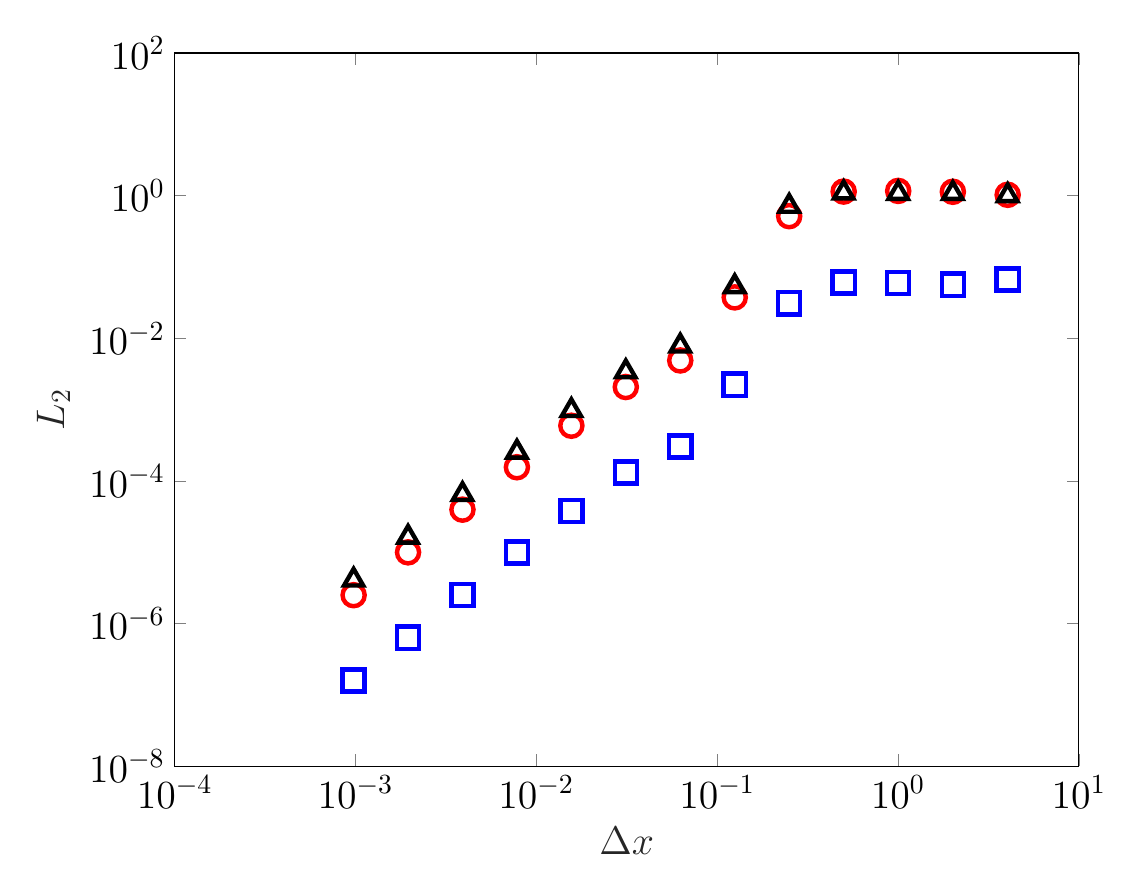
\begin{tikzpicture}
\tikzstyle{every node}=[font=\Large]

\begin{axis}[%
width=4.521in,
height=3.566in,
at={(0.758in,0.481in)},
every axis plot/.append style={ultra thick},
scale only axis,
xmode=log,
xmin=0.0001,
xmax=10,
xtick={0.0001,  0.001,   0.01,    0.1,      1,     10},
xminorticks=false,
xlabel style={font=\color{white!15!black}},
xlabel={\Large $\Delta x$},
ymode=log,
ymin=1e-08,
ymax=100,
ytick={ 1e-08,  1e-06, 0.0001,   0.01,      1,    100},
yminorticks=false,
ylabel style={font=\color{white!15!black}},
ylabel={\Large $L_2$},
axis background/.style={fill=white}
]
 \logLogSlopeTriangle{0.5}{0.2}{0.1}{2}{black};

\addplot [color=blue, draw=none, mark=square, mark size=4pt, mark options={solid, blue}, forget plot]
  table[row sep=crcr]{%
4.04040404040404	0.0667977316044187\\
2.01005025125628	0.0565251008982736\\
1.00250626566416	0.0600244047801842\\
0.500625782227785	0.060369043216863\\
0.250156347717323	0.031027562703989\\
0.125039074710847	0.00223720174663375\\
0.0625097671511174	0.000303213411708855\\
0.0312524415969998	0.00013195585438531\\
0.0156256103754053	3.78678120338089e-05\\
0.00781265259087092	9.90901359842452e-06\\
0.00390628814734519	2.52150220729934e-06\\
0.00195313453678973	6.35217079986901e-07\\
0.000976564884191612	1.59353271500116e-07\\
};
\addplot [color=red, draw=none, mark=o, mark size=4pt, mark options={solid, red}, forget plot]
  table[row sep=crcr]{%
4.04040404040404	1.02894168607817\\
2.01005025125628	1.13471870525711\\
1.00250626566416	1.16651134393852\\
0.500625782227785	1.14209935315627\\
0.250156347717323	0.516295949213657\\
0.125039074710847	0.0375055631709394\\
0.0625097671511174	0.0048956232734942\\
0.0312524415969998	0.00207713643544563\\
0.0156256103754053	0.000595469107815693\\
0.00781265259087092	0.00015580109802979\\
0.00390628814734519	3.96453330936357e-05\\
0.00195313453678973	9.98742874615667e-06\\
0.000976564884191612	2.5054904543415e-06\\
};
\addplot [color=black, draw=none, mark=triangle, mark size=4pt, mark options={solid, black}, forget plot]
  table[row sep=crcr]{%
4.04040404040404	1.00510027333734\\
2.01005025125628	1.07752750295002\\
1.00250626566416	1.07983904140976\\
0.500625782227785	1.09869881739817\\
0.250156347717323	0.712184449316794\\
0.125039074710847	0.05307095900171\\
0.0625097671511174	0.00781225049904385\\
0.0312524415969998	0.00340272133918679\\
0.0156256103754053	0.00097359240010264\\
0.00781265259087092	0.000254452413381455\\
0.00390628814734519	6.47146749585668e-05\\
0.00195313453678973	1.62988208772404e-05\\
0.000976564884191612	4.08829473005837e-06\\
};
%\addplot [color=mycolor1, forget plot]
%  table[row sep=crcr]{%
%4.04040404040404	16.3248648097133\\
%2.01005025125628	4.04030201257544\\
%1.00250626566416	1.0050188126959\\
%0.500625782227785	0.250626173831181\\
%0.250156347717323	0.0625781983032704\\
%0.125039074710847	0.0156347702045448\\
%0.0625097671511174	0.00390747098928691\\
%0.0312524415969998	0.000976715105773881\\
%0.0156256103754053	0.000244159699603973\\
%0.00781265259087092	6.1037540505642e-05\\
%0.00390628814734519	1.52590870900895e-05\\
%0.00195313453678973	3.81473451880083e-06\\
%0.000976564884191612	9.53678973036176e-07\\
%};
\end{axis}
\end{tikzpicture}%
\end{document}
	\caption{$L_2$ comparing numerical solution and forced soluiton}
\end{figure}


\subsection{Analytic Solution}
\subsubsection{Solitary Travelling Wave - Serre ($\beta_1=\beta_2 =0$) }
When $\beta_1 = \beta_2 = 0$ the gSGN are equivalent to the SGN equations which admit the following travelling wave solution

\begin{subequations}
	\begin{equation}
	h(x,t) = a_0 + a_1 \text{sech}^2\left( \kappa (x - ct) \right)
	\end{equation}
	\begin{equation}
	u(x,t) = c \left( 1- \dfrac{a_0}{h(x,t)} \right)
	\end{equation}
	where
	\begin{equation}
	\kappa = \dfrac{\sqrt{3a_1}}{2a_0 \sqrt{a_0 + a_1}}
	\end{equation}
	\begin{equation}
	c = \sqrt{g\left(a_0 + a_1\right)}
	\end{equation}
\end{subequations}

\begin{figure}
	\tikzset{every picture/.style={scale=0.9}}%
	\centering
	\begin{subfigure}{0.49\textwidth}
	\centering
	% This file was created by matlab2tikz.
%
%The latest updates can be retrieved from
%  http://www.mathworks.com/matlabcentral/fileexchange/22022-matlab2tikz-matlab2tikz
%where you can also make suggestions and rate matlab2tikz.
%
\begin{tikzpicture}

\begin{axis}[%
width=4.521in,
height=3.566in,
at={(0.758in,0.481in)},
scale only axis,
xmin=-50,
xmax=100,
xtick={-50,   0,  50, 100},
xlabel style={font=\color{white!15!black}},
xlabel={x (m)},
ymin=0.9,
ymax=1.6,
ytick={  1, 1.2, 1.4, 1.6},
ylabel style={font=\color{white!15!black}},
ylabel={h (m)},
axis background/.style={fill=white}
]
\addplot [color=blue, forget plot]
  table[row sep=crcr]{%
-50.2813379180994	1\\
-50.0468896530166	1\\
-49.8124413879337	1\\
-49.5779931228509	1\\
-49.3435448577681	1\\
-49.1090965926852	1\\
-48.8746483276024	1\\
-48.6402000625195	1\\
-48.4057517974367	1\\
-48.1713035323539	1\\
-47.936855267271	1\\
-47.7024070021882	1\\
-47.4679587371053	1\\
-47.2335104720225	1\\
-46.9990622069397	1\\
-46.7646139418568	1\\
-46.530165676774	1\\
-46.2957174116912	1\\
-46.0612691466083	1\\
-45.8268208815255	1\\
-45.5923726164426	1\\
-45.3579243513598	1\\
-45.123476086277	1\\
-44.8890278211941	1\\
-44.6545795561113	1\\
-44.4201312910284	1\\
-44.1856830259456	1\\
-43.9512347608628	1\\
-43.7167864957799	1\\
-43.4823382306971	1\\
-43.2478899656143	1\\
-43.0134417005314	1\\
-42.7789934354486	1\\
-42.5445451703657	1\\
-42.3100969052829	1\\
-42.0756486402001	1\\
-41.8412003751172	1\\
-41.6067521100344	1\\
-41.3723038449515	1\\
-41.1378555798687	1\\
-40.9034073147859	1\\
-40.668959049703	1\\
-40.4345107846202	1\\
-40.2000625195374	1\\
-39.9656142544545	1\\
-39.7311659893717	1\\
-39.4967177242888	1\\
-39.262269459206	1\\
-39.0278211941232	1\\
-38.7933729290403	1\\
-38.5589246639575	1\\
-38.3244763988747	1\\
-38.0900281337918	1\\
-37.855579868709	1\\
-37.6211316036261	1\\
-37.3866833385433	1\\
-37.1522350734605	1\\
-36.9177868083776	1\\
-36.6833385432948	1\\
-36.4488902782119	1\\
-36.2144420131291	1\\
-35.9799937480463	1\\
-35.7455454829634	1.00000000000001\\
-35.5110972178806	1.00000000000001\\
-35.2766489527977	1.00000000000002\\
-35.0422006877149	1.00000000000002\\
-34.8077524226321	1.00000000000004\\
-34.5733041575492	1.00000000000005\\
-34.3388558924664	1.00000000000008\\
-34.1044076273836	1.00000000000012\\
-33.8699593623007	1.00000000000018\\
-33.6355110972179	1.00000000000026\\
-33.401062832135	1.00000000000039\\
-33.1666145670522	1.00000000000057\\
-32.9321663019694	1.00000000000084\\
-32.6977180368865	1.00000000000123\\
-32.4632697718037	1.00000000000181\\
-32.2288215067208	1.00000000000264\\
-31.994373241638	1.00000000000385\\
-31.7599249765552	1.00000000000559\\
-31.5254767114723	1.0000000000081\\
-31.2910284463895	1.0000000000117\\
-31.0565801813067	1.00000000001686\\
-30.8221319162238	1.00000000002423\\
-30.587683651141	1.00000000003473\\
-30.3532353860581	1.00000000004965\\
-30.1187871209753	1.00000000007076\\
-29.8843388558925	1.00000000010059\\
-29.6498905908096	1.00000000014259\\
-29.4154423257268	1.00000000020158\\
-29.180994060644	1.00000000028418\\
-28.9465457955611	1.00000000039954\\
-28.7120975304783	1.00000000056018\\
-28.4776492653954	1.00000000078326\\
-28.2432010003126	1.00000000109216\\
-28.0087527352298	1.00000000151871\\
-27.7743044701469	1.00000000210606\\
-27.5398562050641	1.00000000291254\\
-27.3054079399812	1.0000000040168\\
-27.0709596748984	1.00000000552452\\
-26.8365114098156	1.00000000757732\\
-26.6020631447327	1.00000001036438\\
-26.3676148796499	1.00000001413764\\
-26.1331666145671	1.00000001923168\\
-25.8987183494842	1.00000002608938\\
-25.6642700844014	1.0000000352953\\
-25.4298218193185	1.00000004761857\\
-25.1953735542357	1.00000006406816\\
-24.9609252891529	1.00000008596359\\
-24.72647702407	1.00000011502529\\
-24.4920287589872	1.00000015348945\\
-24.2575804939043	1.00000020425381\\
-24.0231322288215	1.00000027106174\\
-23.7886839637387	1.00000035873413\\
-23.5542356986558	1.00000047346035\\
-23.319787433573	1.00000062316199\\
-23.0853391684902	1.00000081794618\\
-22.8508909034073	1.00000107066827\\
-22.6164426383245	1.00000139762789\\
-22.3819943732416	1.00000181942692\\
-22.1475461081588	1.0000023620229\\
-21.913097843076	1.00000305801787\\
-21.6786495779931	1.00000394822926\\
-21.4442013129103	1.00000508359724\\
-21.2097530478274	1.00000652749182\\
-20.9753047827446	1.00000835849268\\
-20.7408565176618	1.00001067372539\\
-20.5064082525789	1.00001359284963\\
-20.2719599874961	1.00001726280754\\
-20.0375117224133	1.00002186345402\\
-19.8030634573304	1.00002761420516\\
-19.5686151922476	1.00003478185573\\
-19.3341669271647	1.00004368973197\\
-19.0997186620819	1.00005472836075\\
-18.8652703969991	1.00006836785094\\
-18.6308221319162	1.00008517219618\\
-18.3963738668334	1.00010581572006\\
-18.1619256017505	1.00013110189409\\
-17.9274773366677	1.00016198476474\\
-17.6930290715849	1.00019959322775\\
-17.458580806502	1.0002452583839\\
-17.2241325414192	1.00030054420029\\
-16.9896842763364	1.00036728168296\\
-16.7552360112535	1.00044760673918\\
-16.5207877461707	1.00054400186957\\
-16.2863394810878	1.00065934178048\\
-16.051891216005	1.0007969429435\\
-15.8174429509222	1.00096061705131\\
-15.5829946858393	1.0011547282258\\
-15.3485464207565	1.00138425372495\\
-15.1140981556737	1.0016548477687\\
-14.8796498905908	1.00197290796114\\
-14.645201625508	1.0023456436272\\
-14.4107533604251	1.00278114520757\\
-14.1763050953423	1.00328845366785\\
-13.9418568302595	1.00387762867878\\
-13.7074085651766	1.00455981411803\\
-13.4729603000938	1.00534729923322\\
-13.2385120350109	1.00625357359717\\
-13.0040637699281	1.00729337378393\\
-12.7696155048453	1.00848271950624\\
-12.5351672397624	1.00983893678776\\
-12.3007189746796	1.01138066560577\\
-12.0662707095968	1.01312784934003\\
-11.8318224445139	1.01510170331021\\
-11.5973741794311	1.01732465968668\\
-11.3629259143482	1.01982028612648\\
-11.1284776492654	1.02261317562514\\
-10.8940293841826	1.02572880529488\\
-10.6595811190997	1.02919336208441\\
-10.4251328540169	1.03303353385146\\
-10.190684588934	1.03727626468739\\
-9.95623632385121	1.04194847397484\\
-9.72178805876837	1.04707673933045\\
-9.48733979368553	1.05268694434153\\
-9.25289152860269	1.05880389283676\\
-9.01844326351986	1.06545089232737\\
-8.78399499843702	1.07264931019819\\
-8.54954673335418	1.0804181072015\\
-8.31509846827134	1.08877335378647\\
-8.0806502031885	1.09772773576034\\
-7.84620193810566	1.10729005669583\\
-7.61175367302283	1.11746474534576\\
-7.37730540793999	1.12825137706879\\
-7.14285714285715	1.13964421888189\\
-6.90840887777431	1.15163180820559\\
-6.67396061269147	1.16419657562992\\
-6.43951234760863	1.17731452207938\\
-6.20506408252579	1.19095496057201\\
-5.97061581744295	1.20508033233635\\
-5.73616755236011	1.21964610636083\\
-5.50171928727728	1.23460077049871\\
-5.26727102219444	1.24988592104312\\
-5.0328227571116	1.26543645623178\\
-4.79837449202876	1.28118087745916\\
-4.56392622694592	1.29704170009199\\
-4.32947796186308	1.3129359737373\\
-4.09502969678024	1.32877590964158\\
-3.86058143169741	1.34446961065261\\
-3.62613316661457	1.35992189690531\\
-3.39168490153173	1.37503521815484\\
-3.15723663644889	1.38971064153283\\
-2.92278837136605	1.40384890150489\\
-2.68834010628321	1.41735149701592\\
-2.45389184120038	1.43012181927902\\
-2.21944357611754	1.44206629244249\\
-1.9849953110347	1.45309550850012\\
-1.75054704595186	1.46312533732628\\
-1.51609878086902	1.47207799264432\\
-1.28165051578619	1.47988303508748\\
-1.04720225070335	1.486478294289\\
-0.81275398562051	1.49181069313261\\
-0.578305720537671	1.49583695888505\\
-0.343857455454831	1.4985242078866\\
-0.109409190371991	1.49985039275007\\
0.125039074710841	1.49980460356216\\
0.359487339793681	1.49838721733138\\
0.593935604876521	1.49560989281925\\
0.82838386995936	1.49149541085385\\
1.0628321350422	1.48607736318493\\
1.29728040012503	1.47939969582472\\
1.53172866520787	1.47151611555753\\
1.76617693029071	1.46248937082802\\
2.00062519537355	1.45239042047313\\
2.23507346045639	1.44129750569374\\
2.46952172553923	1.42929514222706\\
2.70396999062206	1.41647305084817\\
2.9384182557049	1.40292504507801\\
3.17286652078774	1.38874789529779\\
3.40731478587058	1.37404018836833\\
3.64176305095342	1.3589012013431\\
3.87621131603625	1.34342980696942\\
4.11065958111909	1.32772342742918\\
4.34510784620193	1.31187705122056\\
4.57955611128477	1.2959823262753\\
4.81400437636761	1.28012674039652\\
5.04845264145045	1.26439289794664\\
5.28290090653329	1.2488578994733\\
5.51734917161613	1.23359282869048\\
5.75179743669896	1.21866234898853\\
5.9862457017818	1.20412440948336\\
6.22069396686464	1.19003005857757\\
6.45514223194748	1.1764233611373\\
6.68959049703032	1.16334141372086\\
6.92403876211316	1.15081445085613\\
7.158487027196	1.13886603417211\\
7.39293529227884	1.12751331525607\\
7.62738355736168	1.11676736243566\\
7.86183182244451	1.10663354127118\\
8.09628008752735	1.09711193837608\\
8.33072835261019	1.08819781824871\\
8.56517661769303	1.07988210307379\\
8.79962488277587	1.07215186591426\\
9.0340731478587	1.06499082833496\\
9.26852141294154	1.05837985425115\\
9.50296967802438	1.05229743264634\\
9.73741794310722	1.04672014272671\\
9.97186620819006	1.04162309604406\\
10.2063144732729	1.03698035110013\\
10.4407627383557	1.03276529691662\\
10.6752110034386	1.02895100299605\\
10.9096592685214	1.0255105339908\\
11.1441075336042	1.02241722822454\\
11.3785557986871	1.01964493996135\\
11.6130040637699	1.01716824598324\\
11.8474523288528	1.0149626176121\\
12.0819005939356	1.01300455979442\\
12.3163488590184	1.0112717192563\\
12.5507971241013	1.00974296403593\\
12.7852453891841	1.00839843691411\\
13.019693654267	1.00721958539794\\
13.2541419193498	1.00618917097478\\
13.4885901844326	1.00529126035223\\
13.7230384495155	1.00451120134316\\
13.9574867145983	1.00383558595183\\
14.1919349796812	1.00325220307764\\
14.426383244764	1.00274998308377\\
14.6608315098468	1.00231893628901\\
14.8952797749297	1.00195008723815\\
15.1297280400125	1.00163540639697\\
15.3641763050953	1.00136774070769\\
15.5986245701782	1.00114074423417\\
15.833072835261	1.00094880992829\\
16.0675211003439	1.00078700336147\\
16.3019693654267	1.00065099909212\\
16.5364176305095	1.00053702018171\\
16.7708658955924	1.00044178123018\\
17.0053141606752	1.00036243517649\\
17.239762425758	1.00029652400162\\
17.4742106908409	1.0002419333792\\
17.7086589559237	1.00019685124205\\
17.9431072210066	1.00015973017075\\
18.1775554860894	1.00012925346107\\
18.4120037511722	1.00010430468965\\
18.6464520162551	1.00008394057076\\
18.8809002813379	1.00006736687926\\
19.1153485464207	1.00005391720483\\
19.3497968115036	1.00004303429953\\
19.5842450765864	1.00003425378251\\
19.8186933416693	1.00002718997212\\
20.0531416067521	1.00002152362502\\
20.2875898718349	1.00001699137406\\
20.5220381369178	1.00001337667\\
20.7564864020006	1.00001050204693\\
20.9909346670835	1.00000822254624\\
21.2253829321663	1.00000642014923\\
21.4598311972491	1.00000499908303\\
21.694279462332	1.00000388187911\\
21.9287277274148	1.00000300607693\\
22.1631759924977	1.00000232147817\\
22.3976242575805	1.00000178786839\\
22.6320725226633	1.00000137313399\\
22.8665207877462	1.00000105171173\\
23.100969052829	1.00000080331698\\
23.3354173179118	1.00000061190444\\
23.5698655829947	1.00000046482201\\
23.8043138480775	1.00000035212447\\
24.0387621131604	1.00000026601869\\
24.2732103782432	1.00000020041698\\
24.507658643326	1.00000015057862\\
24.7421069084089	1.00000011282323\\
24.9765551734917	1.00000008430245\\
25.2110034385746	1.00000006281861\\
25.4454517036574	1.00000004668129\\
25.6798999687402	1.00000003459424\\
25.9143482338231	1.00000002556649\\
26.1487964989059	1.00000001884278\\
26.3832447639887	1.00000001384921\\
26.6176930290716	1.00000001015107\\
26.8521412941544	1.00000000742002\\
27.0865895592373	1.00000000540884\\
27.3210378243201	1.00000000393197\\
27.5554860894029	1.00000000285051\\
27.7899343544858	1.00000000206083\\
28.0243826195686	1.00000000148582\\
28.2588308846514	1.00000000106831\\
28.4932791497343	1.00000000076601\\
28.7277274148171	1.00000000054775\\
28.9621756799	1.0000000003906\\
29.1966239449828	1.00000000027777\\
29.4310722100656	1.00000000019699\\
29.6655204751485	1.00000000013932\\
29.8999687402313	1.00000000009827\\
30.1344170053141	1.00000000006912\\
30.368865270397	1.00000000004848\\
30.6033135354798	1.00000000003391\\
30.8377618005627	1.00000000002366\\
31.0722100656455	1.00000000001646\\
31.3066583307284	1.00000000001142\\
31.5411065958112	1.0000000000079\\
31.775554860894	1.00000000000545\\
32.0100031259769	1.00000000000375\\
32.2444513910597	1.00000000000257\\
32.4788996561425	1.00000000000176\\
32.7133479212254	1.0000000000012\\
32.9477961863082	1.00000000000082\\
33.1822444513911	1.00000000000056\\
33.4166927164739	1.00000000000038\\
33.6511409815567	1.00000000000025\\
33.8855892466396	1.00000000000017\\
34.1200375117224	1.00000000000011\\
34.3544857768052	1.00000000000008\\
34.5889340418881	1.00000000000005\\
34.8233823069709	1.00000000000003\\
35.0578305720538	1.00000000000002\\
35.2922788371366	1.00000000000001\\
35.5267271022194	1.00000000000001\\
35.7611753673023	1.00000000000001\\
35.9956236323851	1\\
36.230071897468	1\\
36.4645201625508	1\\
36.6989684276336	1\\
36.9334166927165	1\\
37.1678649577993	1\\
37.4023132228821	1\\
37.636761487965	1\\
37.8712097530478	1\\
38.1056580181307	1\\
38.3401062832135	1\\
38.5745545482963	1\\
38.8090028133792	1\\
39.043451078462	1\\
39.2778993435448	1\\
39.5123476086277	1\\
39.7467958737105	1\\
39.9812441387934	1\\
40.2156924038762	1\\
40.450140668959	1\\
40.6845889340419	1\\
40.9190371991247	1\\
41.1534854642076	1\\
41.3879337292904	1\\
41.6223819943732	1\\
41.8568302594561	1\\
42.0912785245389	1\\
42.3257267896218	1\\
42.5601750547046	1\\
42.7946233197874	1\\
43.0290715848703	1\\
43.2635198499531	1\\
43.4979681150359	1\\
43.7324163801188	1\\
43.9668646452016	1\\
44.2013129102845	1\\
44.4357611753673	1\\
44.6702094404501	1\\
44.904657705533	1\\
45.1391059706158	1\\
45.3735542356986	1\\
45.6080025007815	1\\
45.8424507658643	1\\
46.0768990309472	1\\
46.31134729603	1\\
46.5457955611128	1\\
46.7802438261957	1\\
47.0146920912785	1\\
47.2491403563614	1\\
47.4835886214442	1\\
47.718036886527	1\\
47.9524851516099	1\\
48.1869334166927	1\\
48.4213816817755	1\\
48.6558299468584	1\\
48.8902782119412	1\\
49.1247264770241	1\\
49.3591747421069	1\\
49.5936230071897	1\\
49.8280712722726	1\\
50.0625195373554	1\\
50.2969678024383	1\\
50.5314160675211	1\\
50.7658643326039	1\\
51.0003125976868	1\\
51.2347608627696	1\\
51.4692091278525	1\\
51.7036573929353	1\\
51.9381056580181	1\\
52.172553923101	1\\
52.4070021881838	1\\
52.6414504532666	1\\
52.8758987183495	1\\
53.1103469834323	1\\
53.3447952485152	1\\
53.579243513598	1\\
53.8136917786808	1\\
54.0481400437637	1\\
54.2825883088465	1\\
54.5170365739293	1\\
54.7514848390122	1\\
54.985933104095	1\\
55.2203813691779	1\\
55.4548296342607	1\\
55.6892778993435	1\\
55.9237261644264	1\\
56.1581744295092	1\\
56.392622694592	1\\
56.6270709596749	1\\
56.8615192247577	1\\
57.0959674898406	1\\
57.3304157549234	1\\
57.5648640200062	1\\
57.7993122850891	1\\
58.0337605501719	1\\
58.2682088152548	1\\
58.5026570803376	1\\
58.7371053454204	1\\
58.9715536105033	1\\
59.2060018755861	1\\
59.440450140669	1\\
59.6748984057518	1\\
59.9093466708346	1\\
60.1437949359175	1\\
60.3782432010003	1\\
60.6126914660831	1\\
60.847139731166	1\\
61.0815879962488	1\\
61.3160362613317	1\\
61.5504845264145	1\\
61.7849327914973	1\\
62.0193810565802	1\\
62.253829321663	1\\
62.4882775867459	1\\
62.7227258518287	1\\
62.9571741169115	1\\
63.1916223819944	1\\
63.4260706470772	1\\
63.66051891216	1\\
63.8949671772429	1\\
64.1294154423257	1\\
64.3638637074086	1\\
64.5983119724914	1\\
64.8327602375742	1\\
65.0672085026571	1\\
65.3016567677399	1\\
65.5361050328227	1\\
65.7705532979056	1\\
66.0050015629884	1\\
66.2394498280713	1\\
66.4738980931541	1\\
66.7083463582369	1\\
66.9427946233198	1\\
67.1772428884026	1\\
67.4116911534854	1\\
67.6461394185683	1\\
67.8805876836511	1\\
68.115035948734	1\\
68.3494842138168	1\\
68.5839324788997	1\\
68.8183807439825	1\\
69.0528290090653	1\\
69.2872772741482	1\\
69.521725539231	1\\
69.7561738043138	1\\
69.9906220693967	1\\
70.2250703344795	1\\
70.4595185995624	1\\
70.6939668646452	1\\
70.928415129728	1\\
71.1628633948109	1\\
71.3973116598937	1\\
71.6317599249765	1\\
71.8662081900594	1\\
72.1006564551422	1\\
72.3351047202251	1\\
72.5695529853079	1\\
72.8040012503907	1\\
73.0384495154736	1\\
73.2728977805564	1\\
73.5073460456393	1\\
73.7417943107221	1\\
73.9762425758049	1\\
74.2106908408878	1\\
74.4451391059706	1\\
74.6795873710534	1\\
74.9140356361363	1\\
75.1484839012191	1\\
75.382932166302	1\\
75.6173804313848	1\\
75.8518286964676	1\\
76.0862769615505	1\\
76.3207252266333	1\\
76.5551734917161	1\\
76.789621756799	1\\
77.0240700218818	1\\
77.2585182869647	1\\
77.4929665520475	1\\
77.7274148171303	1\\
77.9618630822132	1\\
78.196311347296	1\\
78.4307596123789	1\\
78.6652078774617	1\\
78.8996561425445	1\\
79.1341044076274	1\\
79.3685526727102	1\\
79.603000937793	1\\
79.8374492028759	1\\
80.0718974679587	1\\
80.3063457330416	1\\
80.5407939981244	1\\
80.7752422632072	1\\
81.0096905282901	1\\
81.2441387933729	1\\
81.4785870584558	1\\
81.7130353235386	1\\
81.9474835886214	1\\
82.1819318537043	1\\
82.4163801187871	1\\
82.65082838387	1\\
82.8852766489528	1\\
83.1197249140356	1\\
83.3541731791185	1\\
83.5886214442013	1\\
83.8230697092841	1\\
84.057517974367	1\\
84.2919662394498	1\\
84.5264145045327	1\\
84.7608627696155	1\\
84.9953110346983	1\\
85.2297592997812	1\\
85.464207564864	1\\
85.6986558299469	1\\
85.9331040950297	1\\
86.1675523601125	1\\
86.4020006251954	1\\
86.6364488902782	1\\
86.870897155361	1\\
87.1053454204439	1\\
87.3397936855267	1\\
87.5742419506095	1\\
87.8086902156924	1\\
88.0431384807752	1\\
88.2775867458581	1\\
88.5120350109409	1\\
88.7464832760238	1\\
88.9809315411066	1\\
89.2153798061894	1\\
89.4498280712723	1\\
89.6842763363551	1\\
89.9187246014379	1\\
90.1531728665208	1\\
90.3876211316036	1\\
90.6220693966864	1\\
90.8565176617693	1\\
91.0909659268521	1\\
91.325414191935	1\\
91.5598624570178	1\\
91.7943107221006	1\\
92.0287589871835	1\\
92.2632072522663	1\\
92.4976555173492	1\\
92.732103782432	1\\
92.9665520475149	1\\
93.2010003125977	1\\
93.4354485776805	1\\
93.6698968427634	1\\
93.9043451078462	1\\
94.138793372929	1\\
94.3732416380119	1\\
94.6076899030947	1\\
94.8421381681775	1\\
95.0765864332604	1\\
95.3110346983432	1\\
95.5454829634261	1\\
95.7799312285089	1\\
96.0143794935917	1\\
96.2488277586746	1\\
96.4832760237574	1\\
96.7177242888403	1\\
96.9521725539231	1\\
97.1866208190059	1\\
97.4210690840888	1\\
97.6555173491716	1\\
97.8899656142544	1\\
98.1244138793373	1\\
98.3588621444201	1\\
98.5933104095029	1\\
98.8277586745858	1\\
99.0622069396686	1\\
99.2966552047515	1\\
99.5311034698343	1\\
99.7655517349172	1\\
100	1\\
100.234448265083	1\\
};
\end{axis}
\end{tikzpicture}%
	\caption{$t = 0s$}
	\end{subfigure}
	\begin{subfigure}{0.49\textwidth}
	\centering
	% This file was created by matlab2tikz.
%
%The latest updates can be retrieved from
%  http://www.mathworks.com/matlabcentral/fileexchange/22022-matlab2tikz-matlab2tikz
%where you can also make suggestions and rate matlab2tikz.
%
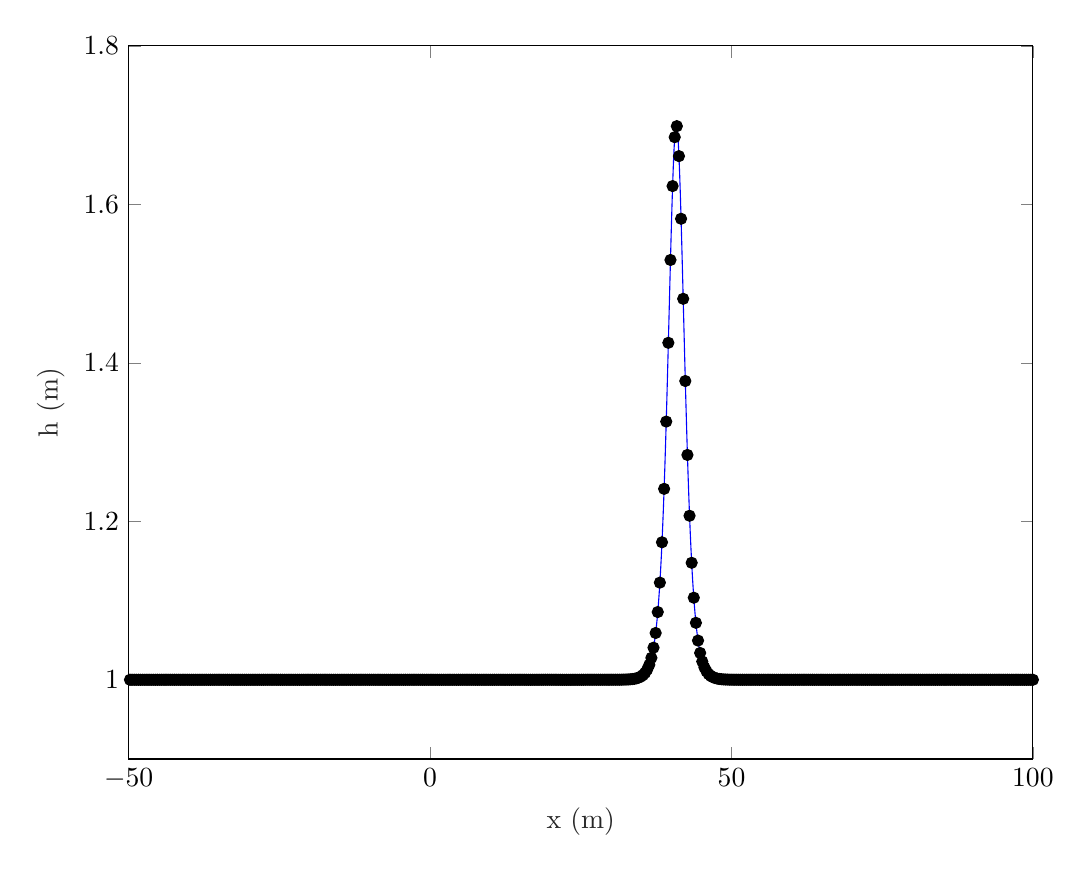
\begin{tikzpicture}

\begin{axis}[%
width=4.521in,
height=3.566in,
at={(0.758in,0.481in)},
scale only axis,
xmin=-50,
xmax=100,
xtick={-50,   0,  50, 100},
xlabel style={font=\color{white!15!black}},
xlabel={x (m)},
ymin=0.9,
ymax=1.8,
ytick={  1, 1.2, 1.4, 1.6, 1.8},
ylabel style={font=\color{white!15!black}},
ylabel={h (m)},
axis background/.style={fill=white}
]
\addplot [color=blue, forget plot]
  table[row sep=crcr]{%
-50.14064697609	1\\
-50.0234411626817	1\\
-49.9062353492733	1\\
-49.789029535865	1\\
-49.6718237224566	1\\
-49.5546179090483	1\\
-49.4374120956399	1\\
-49.3202062822316	1\\
-49.2030004688233	1\\
-49.0857946554149	1\\
-48.9685888420066	1\\
-48.8513830285982	1\\
-48.7341772151899	1\\
-48.6169714017815	1\\
-48.4997655883732	1\\
-48.3825597749648	1\\
-48.2653539615565	1\\
-48.1481481481481	1\\
-48.0309423347398	1\\
-47.9137365213315	1\\
-47.7965307079231	1\\
-47.6793248945148	1\\
-47.5621190811064	1\\
-47.4449132676981	1\\
-47.3277074542897	1\\
-47.2105016408814	1\\
-47.093295827473	1\\
-46.9760900140647	1\\
-46.8588842006564	1\\
-46.741678387248	1\\
-46.6244725738397	1\\
-46.5072667604313	1\\
-46.390060947023	1\\
-46.2728551336146	1\\
-46.1556493202063	1\\
-46.0384435067979	1\\
-45.9212376933896	1\\
-45.8040318799812	1\\
-45.6868260665729	1\\
-45.5696202531646	1\\
-45.4524144397562	1\\
-45.3352086263479	1\\
-45.2180028129395	1\\
-45.1007969995312	1\\
-44.9835911861228	1\\
-44.8663853727145	1\\
-44.7491795593061	1\\
-44.6319737458978	1\\
-44.5147679324894	1\\
-44.3975621190811	1\\
-44.2803563056728	1\\
-44.1631504922644	1\\
-44.0459446788561	1\\
-43.9287388654477	1\\
-43.8115330520394	1\\
-43.694327238631	1\\
-43.5771214252227	1\\
-43.4599156118143	1\\
-43.342709798406	1\\
-43.2255039849977	1\\
-43.1082981715893	1\\
-42.991092358181	1\\
-42.8738865447726	1\\
-42.7566807313643	1\\
-42.6394749179559	1\\
-42.5222691045476	1\\
-42.4050632911392	1\\
-42.2878574777309	1\\
-42.1706516643225	1\\
-42.0534458509142	1\\
-41.9362400375059	1\\
-41.8190342240975	1\\
-41.7018284106892	1\\
-41.5846225972808	1\\
-41.4674167838725	1\\
-41.3502109704641	1\\
-41.2330051570558	1\\
-41.1157993436474	1\\
-40.9985935302391	1\\
-40.8813877168308	1\\
-40.7641819034224	1\\
-40.6469760900141	1\\
-40.5297702766057	1\\
-40.4125644631974	1\\
-40.295358649789	1\\
-40.1781528363807	1\\
-40.0609470229723	1\\
-39.943741209564	1\\
-39.8265353961556	1\\
-39.7093295827473	1\\
-39.592123769339	1\\
-39.4749179559306	1\\
-39.3577121425223	1\\
-39.2405063291139	1\\
-39.1233005157056	1\\
-39.0060947022972	1\\
-38.8888888888889	1\\
-38.7716830754805	1\\
-38.6544772620722	1\\
-38.5372714486639	1\\
-38.4200656352555	1\\
-38.3028598218472	1\\
-38.1856540084388	1\\
-38.0684481950305	1\\
-37.9512423816221	1\\
-37.8340365682138	1\\
-37.7168307548054	1\\
-37.5996249413971	1\\
-37.4824191279887	1\\
-37.3652133145804	1\\
-37.2480075011721	1\\
-37.1308016877637	1\\
-37.0135958743554	1\\
-36.896390060947	1\\
-36.7791842475387	1\\
-36.6619784341303	1\\
-36.544772620722	1\\
-36.4275668073136	1\\
-36.3103609939053	1\\
-36.193155180497	1\\
-36.0759493670886	1\\
-35.9587435536803	1\\
-35.8415377402719	1\\
-35.7243319268636	1\\
-35.6071261134552	1\\
-35.4899203000469	1\\
-35.3727144866385	1\\
-35.2555086732302	1\\
-35.1383028598218	1\\
-35.0210970464135	1\\
-34.9038912330052	1\\
-34.7866854195968	1\\
-34.6694796061885	1\\
-34.5522737927801	1\\
-34.4350679793718	1\\
-34.3178621659634	1\\
-34.2006563525551	1\\
-34.0834505391467	1\\
-33.9662447257384	1\\
-33.8490389123301	1\\
-33.7318330989217	1\\
-33.6146272855134	1\\
-33.497421472105	1\\
-33.3802156586967	1\\
-33.2630098452883	1\\
-33.14580403188	1\\
-33.0285982184716	1\\
-32.9113924050633	1\\
-32.7941865916549	1\\
-32.6769807782466	1\\
-32.5597749648383	1\\
-32.4425691514299	1\\
-32.3253633380216	1\\
-32.2081575246132	1\\
-32.0909517112049	1\\
-31.9737458977965	1\\
-31.8565400843882	1\\
-31.7393342709798	1\\
-31.6221284575715	1\\
-31.5049226441632	1\\
-31.3877168307548	1\\
-31.2705110173465	1\\
-31.1533052039381	1\\
-31.0360993905298	1\\
-30.9188935771214	1\\
-30.8016877637131	1\\
-30.6844819503047	1\\
-30.5672761368964	1\\
-30.450070323488	1\\
-30.3328645100797	1\\
-30.2156586966714	1\\
-30.098452883263	1\\
-29.9812470698547	1\\
-29.8640412564463	1\\
-29.746835443038	1\\
-29.6296296296296	1\\
-29.5124238162213	1\\
-29.3952180028129	1\\
-29.2780121894046	1\\
-29.1608063759962	1\\
-29.0436005625879	1\\
-28.9263947491796	1\\
-28.8091889357712	1\\
-28.6919831223629	1\\
-28.5747773089545	1\\
-28.4575714955462	1\\
-28.3403656821378	1\\
-28.2231598687295	1\\
-28.1059540553211	1\\
-27.9887482419128	1\\
-27.8715424285045	1\\
-27.7543366150961	1\\
-27.6371308016878	1\\
-27.5199249882794	1\\
-27.4027191748711	1\\
-27.2855133614627	1\\
-27.1683075480544	1\\
-27.051101734646	1\\
-26.9338959212377	1\\
-26.8166901078293	1\\
-26.699484294421	1\\
-26.5822784810127	1\\
-26.4650726676043	1\\
-26.347866854196	1\\
-26.2306610407876	1\\
-26.1134552273793	1\\
-25.9962494139709	1\\
-25.8790436005626	1\\
-25.7618377871542	1\\
-25.6446319737459	1\\
-25.5274261603376	1\\
-25.4102203469292	1\\
-25.2930145335209	1\\
-25.1758087201125	1\\
-25.0586029067042	1\\
-24.9413970932958	1\\
-24.8241912798875	1\\
-24.7069854664791	1\\
-24.5897796530708	1\\
-24.4725738396624	1\\
-24.3553680262541	1\\
-24.2381622128458	1\\
-24.1209563994374	1\\
-24.0037505860291	1\\
-23.8865447726207	1\\
-23.7693389592124	1\\
-23.652133145804	1\\
-23.5349273323957	1\\
-23.4177215189873	1\\
-23.300515705579	1\\
-23.1833098921707	1\\
-23.0661040787623	1\\
-22.948898265354	1\\
-22.8316924519456	1\\
-22.7144866385373	1\\
-22.5972808251289	1\\
-22.4800750117206	1\\
-22.3628691983122	1\\
-22.2456633849039	1\\
-22.1284575714955	1\\
-22.0112517580872	1\\
-21.8940459446789	1\\
-21.7768401312705	1\\
-21.6596343178622	1\\
-21.5424285044538	1\\
-21.4252226910455	1\\
-21.3080168776371	1\\
-21.1908110642288	1\\
-21.0736052508204	1\\
-20.9563994374121	1\\
-20.8391936240038	1\\
-20.7219878105954	1\\
-20.6047819971871	1\\
-20.4875761837787	1\\
-20.3703703703704	1\\
-20.253164556962	1\\
-20.1359587435537	1\\
-20.0187529301453	1\\
-19.901547116737	1\\
-19.7843413033286	1\\
-19.6671354899203	1\\
-19.549929676512	1\\
-19.4327238631036	1\\
-19.3155180496953	1\\
-19.1983122362869	1\\
-19.0811064228786	1\\
-18.9639006094702	1\\
-18.8466947960619	1\\
-18.7294889826535	1\\
-18.6122831692452	1\\
-18.4950773558368	1\\
-18.3778715424285	1\\
-18.2606657290202	1\\
-18.1434599156118	1\\
-18.0262541022035	1\\
-17.9090482887951	1\\
-17.7918424753868	1\\
-17.6746366619784	1\\
-17.5574308485701	1\\
-17.4402250351617	1\\
-17.3230192217534	1\\
-17.2058134083451	1\\
-17.0886075949367	1\\
-16.9714017815284	1\\
-16.85419596812	1\\
-16.7369901547117	1\\
-16.6197843413033	1\\
-16.502578527895	1\\
-16.3853727144866	1\\
-16.2681669010783	1\\
-16.1509610876699	1\\
-16.0337552742616	1\\
-15.9165494608533	1\\
-15.7993436474449	1\\
-15.6821378340366	1\\
-15.5649320206282	1\\
-15.4477262072199	1\\
-15.3305203938115	1\\
-15.2133145804032	1\\
-15.0961087669948	1\\
-14.9789029535865	1\\
-14.8616971401782	1\\
-14.7444913267698	1\\
-14.6272855133615	1\\
-14.5100796999531	1\\
-14.3928738865448	1\\
-14.2756680731364	1\\
-14.1584622597281	1\\
-14.0412564463197	1\\
-13.9240506329114	1\\
-13.806844819503	1\\
-13.6896390060947	1\\
-13.5724331926864	1\\
-13.455227379278	1\\
-13.3380215658697	1\\
-13.2208157524613	1\\
-13.103609939053	1\\
-12.9864041256446	1\\
-12.8691983122363	1\\
-12.7519924988279	1\\
-12.6347866854196	1\\
-12.5175808720113	1\\
-12.4003750586029	1\\
-12.2831692451946	1\\
-12.1659634317862	1\\
-12.0487576183779	1\\
-11.9315518049695	1\\
-11.8143459915612	1\\
-11.6971401781528	1\\
-11.5799343647445	1\\
-11.4627285513361	1\\
-11.3455227379278	1\\
-11.2283169245195	1\\
-11.1111111111111	1\\
-10.9939052977028	1\\
-10.8766994842944	1\\
-10.7594936708861	1\\
-10.6422878574777	1\\
-10.5250820440694	1\\
-10.407876230661	1\\
-10.2906704172527	1\\
-10.1734646038444	1\\
-10.056258790436	1\\
-9.93905297702766	1\\
-9.82184716361932	1\\
-9.70464135021097	1\\
-9.58743553680262	1\\
-9.47022972339428	1\\
-9.35302390998594	1\\
-9.23581809657759	1\\
-9.11861228316924	1\\
-9.0014064697609	1\\
-8.88420065635255	1\\
-8.76699484294421	1\\
-8.64978902953587	1\\
-8.53258321612752	1\\
-8.41537740271917	1\\
-8.29817158931083	1\\
-8.18096577590249	1\\
-8.06375996249414	1\\
-7.94655414908579	1\\
-7.82934833567745	1\\
-7.7121425222691	1\\
-7.59493670886076	1\\
-7.47773089545242	1\\
-7.36052508204407	1\\
-7.24331926863572	1\\
-7.12611345522738	1\\
-7.00890764181904	1\\
-6.89170182841069	1\\
-6.77449601500234	1\\
-6.657290201594	1\\
-6.54008438818565	1\\
-6.42287857477731	1\\
-6.30567276136896	1\\
-6.18846694796062	1\\
-6.07126113455227	1\\
-5.95405532114393	1\\
-5.83684950773559	1\\
-5.71964369432724	1\\
-5.60243788091889	1\\
-5.48523206751055	1\\
-5.3680262541022	1\\
-5.25082044069386	1\\
-5.13361462728551	1\\
-5.01640881387717	1\\
-4.89920300046882	1\\
-4.78199718706048	1\\
-4.66479137365214	1\\
-4.54758556024379	1\\
-4.43037974683544	1\\
-4.31317393342709	1\\
-4.19596812001875	1\\
-4.07876230661041	1\\
-3.96155649320206	1\\
-3.84435067979372	1\\
-3.72714486638537	1\\
-3.60993905297703	1\\
-3.49273323956868	1\\
-3.37552742616034	1\\
-3.25832161275199	1\\
-3.14111579934364	1\\
-3.0239099859353	1\\
-2.90670417252696	1\\
-2.78949835911861	1\\
-2.67229254571027	1\\
-2.55508673230192	1\\
-2.43788091889358	1\\
-2.32067510548523	1\\
-2.20346929207689	1\\
-2.08626347866854	1\\
-1.96905766526019	1\\
-1.85185185185185	1\\
-1.73464603844351	1\\
-1.61744022503516	1\\
-1.50023441162681	1\\
-1.38302859821847	1\\
-1.26582278481013	1\\
-1.14861697140178	1\\
-1.03141115799344	1\\
-0.914205344585092	1\\
-0.796999531176745	1\\
-0.679793717768398	1\\
-0.562587904360058	1\\
-0.445382090951711	1\\
-0.328176277543363	1\\
-0.210970464135023	1\\
-0.0937646507266763	1\\
0.0234411626816708	1\\
0.140646976090011	1\\
0.257852789498358	1\\
0.375058602906705	1\\
0.492264416315052	1\\
0.609470229723392	1\\
0.726676043131739	1\\
0.843881856540087	1\\
0.961087669948427	1\\
1.07829348335677	1\\
1.19549929676512	1\\
1.31270511017347	1\\
1.42991092358181	1\\
1.54711673699016	1\\
1.6643225503985	1\\
1.78152836380684	1\\
1.89873417721519	1\\
2.01593999062354	1\\
2.13314580403188	1\\
2.25035161744022	1\\
2.36755743084857	1\\
2.48476324425692	1\\
2.60196905766526	1\\
2.71917487107361	1\\
2.83638068448195	1\\
2.95358649789029	1\\
3.07079231129864	1\\
3.18799812470699	1\\
3.30520393811533	1\\
3.42240975152367	1\\
3.53961556493202	1\\
3.65682137834037	1\\
3.77402719174871	1\\
3.89123300515705	1\\
4.0084388185654	1\\
4.12564463197375	1\\
4.24285044538209	1\\
4.36005625879044	1\\
4.47726207219878	1\\
4.59446788560712	1\\
4.71167369901547	1\\
4.82887951242382	1\\
4.94608532583216	1\\
5.0632911392405	1\\
5.18049695264885	1\\
5.2977027660572	1\\
5.41490857946554	1\\
5.53211439287389	1\\
5.64932020628223	1\\
5.76652601969058	1\\
5.88373183309892	1\\
6.00093764650727	1\\
6.11814345991561	1\\
6.23534927332395	1\\
6.3525550867323	1\\
6.46976090014065	1\\
6.58696671354899	1\\
6.70417252695734	1\\
6.82137834036568	1\\
6.93858415377403	1\\
7.05578996718237	1\\
7.17299578059072	1\\
7.29020159399906	1\\
7.4074074074074	1\\
7.52461322081575	1\\
7.6418190342241	1\\
7.75902484763245	1\\
7.87623066104079	1\\
7.99343647444913	1\\
8.11064228785748	1\\
8.22784810126582	1\\
8.34505391467417	1\\
8.46225972808251	1\\
8.57946554149086	1\\
8.6966713548992	1\\
8.81387716830755	1\\
8.9310829817159	1\\
9.04828879512424	1\\
9.16549460853258	1\\
9.28270042194093	1\\
9.39990623534927	1\\
9.51711204875762	1\\
9.63431786216596	1\\
9.75152367557431	1\\
9.86872948898265	1\\
9.985935302391	1\\
10.1031411157993	1\\
10.2203469292077	1\\
10.337552742616	1.00000000000001\\
10.4547585560244	1.00000000000001\\
10.5719643694327	1.00000000000001\\
10.6891701828411	1.00000000000001\\
10.8063759962494	1.00000000000001\\
10.9235818096578	1.00000000000001\\
11.0407876230661	1.00000000000001\\
11.1579934364744	1.00000000000001\\
11.2751992498828	1.00000000000001\\
11.3924050632911	1.00000000000002\\
11.5096108766995	1.00000000000002\\
11.6268166901078	1.00000000000002\\
11.7440225035162	1.00000000000003\\
11.8612283169245	1.00000000000003\\
11.9784341303329	1.00000000000003\\
12.0956399437412	1.00000000000004\\
12.2128457571496	1.00000000000004\\
12.3300515705579	1.00000000000005\\
12.4472573839662	1.00000000000005\\
12.5644631973746	1.00000000000006\\
12.6816690107829	1.00000000000007\\
12.7988748241913	1.00000000000008\\
12.9160806375996	1.00000000000009\\
13.033286451008	1.00000000000011\\
13.1504922644163	1.00000000000012\\
13.2676980778247	1.00000000000014\\
13.384903891233	1.00000000000016\\
13.5021097046413	1.00000000000018\\
13.6193155180497	1.0000000000002\\
13.736521331458	1.00000000000023\\
13.8537271448664	1.00000000000026\\
13.9709329582747	1.0000000000003\\
14.0881387716831	1.00000000000034\\
14.2053445850914	1.00000000000039\\
14.3225503984998	1.00000000000044\\
14.4397562119081	1.0000000000005\\
14.5569620253165	1.00000000000057\\
14.6741678387248	1.00000000000065\\
14.7913736521331	1.00000000000074\\
14.9085794655415	1.00000000000085\\
15.0257852789498	1.00000000000096\\
15.1429910923582	1.0000000000011\\
15.2601969057665	1.00000000000125\\
15.3774027191749	1.00000000000142\\
15.4946085325832	1.00000000000162\\
15.6118143459916	1.00000000000185\\
15.7290201593999	1.00000000000211\\
15.8462259728083	1.0000000000024\\
15.9634317862166	1.00000000000273\\
16.0806375996249	1.00000000000311\\
16.1978434130333	1.00000000000354\\
16.3150492264416	1.00000000000404\\
16.43225503985	1.0000000000046\\
16.5494608532583	1.00000000000524\\
16.6666666666667	1.00000000000597\\
16.783872480075	1.0000000000068\\
16.9010782934834	1.00000000000775\\
17.0182841068917	1.00000000000882\\
17.1354899203	1.00000000001005\\
17.2526957337084	1.00000000001145\\
17.3699015471167	1.00000000001304\\
17.4871073605251	1.00000000001486\\
17.6043131739334	1.00000000001692\\
17.7215189873418	1.00000000001928\\
17.8387248007501	1.00000000002196\\
17.9559306141585	1.00000000002502\\
18.0731364275668	1.0000000000285\\
18.1903422409752	1.00000000003246\\
18.3075480543835	1.00000000003698\\
18.4247538677918	1.00000000004212\\
18.5419596812002	1.00000000004798\\
18.6591654946085	1.00000000005466\\
18.7763713080169	1.00000000006226\\
18.8935771214252	1.00000000007093\\
19.0107829348336	1.00000000008079\\
19.1279887482419	1.00000000009204\\
19.2451945616503	1.00000000010484\\
19.3624003750586	1.00000000011943\\
19.4796061884669	1.00000000013604\\
19.5968120018753	1.00000000015497\\
19.7140178152836	1.00000000017653\\
19.831223628692	1.00000000020109\\
19.9484294421003	1.00000000022907\\
20.0656352555087	1.00000000026094\\
20.182841068917	1.00000000029725\\
20.3000468823254	1.00000000033861\\
20.4172526957337	1.00000000038572\\
20.5344585091421	1.00000000043938\\
20.6516643225504	1.00000000050052\\
20.7688701359587	1.00000000057015\\
20.8860759493671	1.00000000064948\\
21.0032817627754	1.00000000073985\\
21.1204875761838	1.00000000084278\\
21.2376933895921	1.00000000096004\\
21.3548992030005	1.00000000109361\\
21.4721050164088	1.00000000124577\\
21.5893108298172	1.0000000014191\\
21.7065166432255	1.00000000161654\\
21.8237224566338	1.00000000184145\\
21.9409282700422	1.00000000209766\\
22.0581340834505	1.00000000238951\\
22.1753398968589	1.00000000272197\\
22.2925457102672	1.00000000310068\\
22.4097515236756	1.00000000353209\\
22.5269573370839	1.00000000402352\\
22.6441631504923	1.00000000458332\\
22.7613689639006	1.00000000522101\\
22.878574777309	1.00000000594742\\
22.9957805907173	1.0000000067749\\
23.1129864041256	1.00000000771751\\
23.230192217534	1.00000000879126\\
23.3473980309423	1.00000001001441\\
23.4646038443507	1.00000001140774\\
23.581809657759	1.00000001299493\\
23.6990154711674	1.00000001480295\\
23.8162212845757	1.00000001686252\\
23.9334270979841	1.00000001920864\\
24.0506329113924	1.00000002188119\\
24.1678387248007	1.00000002492557\\
24.2850445382091	1.00000002839353\\
24.4022503516174	1.00000003234399\\
24.5194561650258	1.00000003684409\\
24.6366619784341	1.00000004197029\\
24.7538677918425	1.00000004780973\\
24.8710736052508	1.00000005446161\\
24.9882794186592	1.00000006203899\\
25.1054852320675	1.00000007067062\\
25.2226910454759	1.0000000805032\\
25.3398968588842	1.00000009170381\\
25.4571026722925	1.00000010446279\\
25.5743084857009	1.00000011899695\\
25.6915142991092	1.00000013555329\\
25.8087201125176	1.00000015441315\\
25.9259259259259	1.00000017589703\\
26.0431317393343	1.00000020037001\\
26.1603375527426	1.00000022824798\\
26.277543366151	1.00000026000468\\
26.3947491795593	1.00000029617977\\
26.5119549929676	1.00000033738798\\
26.629160806376	1.00000038432959\\
26.7463666197843	1.0000004378023\\
26.8635724331927	1.00000049871479\\
26.980778246601	1.00000056810218\\
27.0979840600094	1.0000006471436\\
27.2151898734177	1.00000073718224\\
27.3323956868261	1.00000083974816\\
27.4496015002344	1.00000095658431\\
27.5668073136428	1.00000108967614\\
27.6840131270511	1.00000124128534\\
27.8012189404594	1.00000141398825\\
27.9184247538678	1.0000016107197\\
28.0356305672761	1.00000183482281\\
28.1528363806845	1.00000209010585\\
28.2700421940928	1.00000238090694\\
28.3872480075012	1.00000271216775\\
28.5044538209095	1.00000308951751\\
28.6216596343179	1.00000351936862\\
28.7388654477262	1.00000400902566\\
28.8560712611346	1.00000456680947\\
28.9732770745429	1.00000520219857\\
29.0904828879512	1.00000592599023\\
29.2076887013596	1.00000675048389\\
29.3248945147679	1.0000076896902\\
29.4421003281763	1.00000875956908\\
29.5593061415846	1.00000997830084\\
29.676511954993	1.00001136659518\\
29.7937177684013	1.00001294804298\\
29.9109235818097	1.00001474951715\\
30.028129395218	1.00001680162923\\
30.1453352086263	1.00001913924939\\
30.2625410220347	1.00002180209889\\
30.379746835443	1.00002483542488\\
30.4969526488514	1.00002829076897\\
30.6141584622597	1.00003222684283\\
30.7313642756681	1.00003671052539\\
30.8485700890764	1.00004181799877\\
30.9657759024848	1.00004763604212\\
31.0829817158931	1.00005426350526\\
31.2001875293015	1.00006181298725\\
31.3173933427098	1.00007041274808\\
31.4345991561181	1.00008020888611\\
31.5518049695265	1.00009136781794\\
31.6690107829348	1.00010407910273\\
31.7862165963432	1.00011855865867\\
31.9034224097515	1.00013505242597\\
32.0206282231599	1.00015384053823\\
32.1378340365682	1.00017524207239\\
32.2550398499766	1.00019962045743\\
32.3722456633849	1.00022738963267\\
32.4894514767932	1.00025902105926\\
32.6066572902016	1.00029505170228\\
32.7238631036099	1.00033609311725\\
32.8410689170183	1.0003828417927\\
32.9582747304266	1.00043609092128\\
33.075480543835	1.00049674379492\\
33.1926863572433	1.00056582904603\\
33.3098921706517	1.00064451798632\\
33.42709798406	1.00073414432823\\
33.5443037974684	1.00083622661165\\
33.6615096108767	1.00095249370097\\
33.778715424285	1.0010849137646\\
33.8959212376934	1.00123572720247\\
34.0131270511017	1.00140748404565\\
34.1303328645101	1.00160308641825\\
34.2475386779184	1.00182583672379\\
34.3647444913268	1.00207949229868\\
34.4819503047351	1.00236832736205\\
34.5991561181435	1.00269720318669\\
34.7163619315518	1.00307164751712\\
34.8335677449601	1.00349794436982\\
34.9507735583685	1.00398323546349\\
35.0679793717768	1.00453563464401\\
35.1851851851852	1.00516435678464\\
35.3023909985935	1.00587986275291\\
35.4195968120019	1.00669402213515\\
35.5368026254102	1.00762029548797\\
35.6540084388186	1.00867393793132\\
35.7712142522269	1.00987222589332\\
35.8884200656353	1.0112347087405\\
36.0056258790436	1.01278348685073\\
36.122831692452	1.01454351737156\\
36.2400375058603	1.01654294840809\\
36.3572433192686	1.01881348163989\\
36.474449132677	1.02139076230266\\
36.5916549460853	1.02431479399257\\
36.7088607594937	1.02763037374657\\
36.826066572902	1.03138754018544\\
36.9432723863104	1.03564202401603\\
37.0604781997187	1.04045568569542\\
37.177684013127	1.04589691935839\\
37.2948898265354	1.05204099499315\\
37.4120956399437	1.05897030211297\\
37.5293014533521	1.06677444764938\\
37.6465072667604	1.07555014839734\\
37.7637130801688	1.08540084413538\\
37.8809188935771	1.09643594181754\\
37.9981247069855	1.10876958464425\\
38.1153305203938	1.12251882353235\\
38.2325363338022	1.13780105438818\\
38.3497421472105	1.15473057541087\\
38.4669479606189	1.17341411827757\\
38.5841537740272	1.1939452205691\\
38.7013595874355	1.21639734045667\\
38.8185654008439	1.24081567565857\\
38.9357712142522	1.26720774434257\\
39.0529770276606	1.2955329222128\\
39.1701828410689	1.32569131053987\\
39.2873886544773	1.35751253148912\\
39.4045944678856	1.390745297658\\
39.5218002812939	1.42504885763197\\
39.6390060947023	1.45998763933329\\
39.7562119081106	1.49503054446875\\
39.873417721519	1.52955632751224\\
39.9906235349273	1.56286625940054\\
40.1078293483357	1.59420478473859\\
40.225035161744	1.62278812430555\\
40.3422409751524	1.64783980054667\\
40.4594467885607	1.66863098727213\\
40.5766526019691	1.68452258078498\\
40.6938584153774	1.69500516570792\\
40.8110642287858	1.69973279861715\\
40.9282700421941	1.69854688081361\\
41.0454758556024	1.69148734707972\\
41.1626816690108	1.67878983410198\\
41.2798874824191	1.66086916888311\\
41.3970932958275	1.63829113257875\\
41.5142991092358	1.61173572291671\\
41.6315049226442	1.58195585851466\\
41.7487107360525	1.54973556893153\\
41.8659165494608	1.51585125455816\\
41.9831223628692	1.48103873924162\\
42.1003281762775	1.44596778161234\\
42.2175339896859	1.41122465757309\\
42.3347398030942	1.3773025291539\\
42.4519456165026	1.34459866185464\\
42.5691514299109	1.3134171679134\\
42.6863572433193	1.28397581179477\\
42.8035630567276	1.25641546268183\\
42.920768870136	1.23081095285464\\
43.0379746835443	1.20718234045221\\
43.1551804969527	1.18550583214261\\
43.272386310361	1.16572386238546\\
43.3895921237693	1.14775403199658\\
43.5067979371777	1.13149677160441\\
43.624003750586	1.11684171519414\\
43.7412095639944	1.10367284988357\\
43.8584153774027	1.09187255723844\\
43.9756211908111	1.08132468621399\\
44.0928270042194	1.07191680507409\\
44.2100328176277	1.06354177520369\\
44.3272386310361	1.05609877817921\\
44.4444444444444	1.04949391219976\\
44.5616502578528	1.04364045739367\\
44.6788560712611	1.03845889316303\\
44.7960618846695	1.033876735555\\
44.9132676980778	1.02982824914637\\
45.0304735114862	1.02625407628462\\
45.1476793248945	1.02310081673667\\
45.2648851383029	1.02032058273039\\
45.3820909517112	1.01787054784875\\
45.4992967651196	1.01571250304345\\
45.6165025785279	1.01381242896519\\
45.7337083919362	1.01214009066847\\
45.8509142053446	1.01066865836391\\
45.9681200187529	1.00937435611301\\
46.0853258321613	1.00823613906005\\
46.2025316455696	1.00723539886986\\
46.319737458978	1.00635569640231\\
46.4369432723863	1.0055825202356\\
46.5541490857947	1.0049030693964\\
46.671354899203	1.00430605852224\\
46.7885607126113	1.00378154363688\\
46.9057665260197	1.00332076673743\\
47.022972339428	1.0029160174518\\
47.1401781528364	1.00256051011353\\
47.2573839662447	1.00224827470599\\
47.3745897796531	1.00197406024124\\
47.4917955930614	1.00173324925606\\
47.6090014064698	1.00152178222268\\
47.7262072198781	1.00133609078359\\
47.8434130332865	1.00117303882565\\
47.9606188466948	1.00102987050806\\
48.0778246601031	1.00090416445011\\
48.1950304735115	1.00079379336951\\
48.3122362869198	1.0006968885386\\
48.4294421003282	1.00061180849548\\
48.5466479137365	1.00053711151023\\
48.6638537271449	1.00047153136275\\
48.7810595405532	1.00041395603937\\
48.8982653539616	1.00036340900106\\
49.0154711673699	1.00031903271587\\
49.1326769807782	1.0002800741846\\
49.2498827941866	1.00024587222034\\
49.3670886075949	1.00021584627088\\
49.4842944210033	1.00018948659805\\
49.6015002344116	1.00016634565013\\
49.71870604782	1.00014603048306\\
49.8359118612283	1.00012819610352\\
49.9531176746367	1.00011253962214\\
50.070323488045	1.00009879511859\\
50.1875293014534	1.00008672913208\\
50.3047351148617	1.00007613670128\\
50.42194092827	1.00006683788695\\
50.5391467416784	1.0000586747184\\
50.6563525550867	1.00005150851238\\
50.7735583684951	1.00004521751891\\
50.8907641819034	1.0000396948543\\
51.0079699953118	1.00003484668635\\
51.1251758087201	1.00003059064095\\
51.2423816221285	1.00002685440323\\
51.3595874355368	1.0000235744893\\
51.4767932489451	1.00002069516802\\
51.5939990623535	1.00001816751431\\
51.7112048757618	1.00001594857809\\
51.8284106891702	1.00001400065467\\
51.9456165025785	1.00001229064413\\
52.0628223159869	1.00001078948908\\
52.1800281293952	1.00000947168091\\
52.2972339428036	1.00000831482643\\
52.4144397562119	1.00000729926738\\
52.5316455696203	1.00000640774646\\
52.6488513830286	1.00000562511405\\
52.7660571964369	1.00000493807084\\
52.8832630098453	1.00000433494182\\
53.0004688232536	1.00000380547792\\
53.117674636662	1.00000334068188\\
53.2348804500703	1.00000293265529\\
53.3520862634787	1.00000257446445\\
53.469292076887	1.00000226002252\\
53.5864978902954	1.00000198398609\\
53.7037037037037	1.00000174166437\\
53.820909517112	1.00000152893951\\
53.9381153305204	1.00000134219659\\
54.0553211439287	1.00000117826222\\
54.1725269573371	1.00000103435059\\
54.2897327707454	1.00000090801616\\
54.4069385841538	1.00000079711206\\
54.5241443975621	1.00000069975366\\
54.6413502109705	1.00000061428651\\
54.7585560243788	1.00000053925822\\
54.8757618377872	1.0000004733938\\
54.9929676511955	1.00000041557398\\
55.1101734646038	1.00000036481622\\
55.2273792780122	1.00000032025795\\
55.3445850914205	1.00000028114198\\
55.4617909048289	1.0000002468036\\
55.5789967182372	1.00000021665926\\
55.6962025316456	1.00000019019673\\
55.8134083450539	1.0000001669663\\
55.9306141584623	1.00000014657321\\
56.0478199718706	1.00000012867091\\
56.165025785279	1.00000011295518\\
56.2822315986873	1.00000009915895\\
56.3994374120956	1.00000008704778\\
56.516643225504	1.00000007641585\\
56.6338490389123	1.0000000670825\\
56.7510548523207	1.00000005888911\\
56.868260665729	1.00000005169646\\
56.9854664791374	1.00000004538231\\
57.1026722925457	1.00000003983936\\
57.2198781059541	1.00000003497342\\
57.3370839193624	1.0000000307018\\
57.4542897327707	1.00000002695192\\
57.5714955461791	1.00000002366004\\
57.6887013595874	1.00000002077022\\
57.8059071729958	1.00000001823337\\
57.9231129864041	1.00000001600637\\
58.0403187998125	1.00000001405136\\
58.1575246132208	1.00000001233515\\
58.2747304266292	1.00000001082854\\
58.3919362400375	1.00000000950596\\
58.5091420534459	1.00000000834491\\
58.6263478668542	1.00000000732567\\
58.7435536802625	1.00000000643092\\
58.8607594936709	1.00000000564545\\
58.9779653070792	1.00000000495592\\
59.0951711204876	1.00000000435061\\
59.2123769338959	1.00000000381923\\
59.3295827473043	1.00000000335276\\
59.4467885607126	1.00000000294325\\
59.563994374121	1.00000000258377\\
59.6812001875293	1.00000000226819\\
59.7984060009376	1.00000000199116\\
59.915611814346	1.00000000174796\\
60.0328176277543	1.00000000153446\\
60.1500234411627	1.00000000134705\\
60.267229254571	1.00000000118252\\
60.3844350679794	1.00000000103809\\
60.5016408813877	1.0000000009113\\
60.6188466947961	1.00000000079999\\
60.7360525082044	1.00000000070228\\
60.8532583216128	1.00000000061651\\
60.9704641350211	1.00000000054121\\
61.0876699484294	1.0000000004751\\
61.2048757618378	1.00000000041708\\
61.3220815752461	1.00000000036613\\
61.4392873886545	1.00000000032141\\
61.5564932020628	1.00000000028216\\
61.6736990154712	1.00000000024769\\
61.7909048288795	1.00000000021744\\
61.9081106422879	1.00000000019088\\
62.0253164556962	1.00000000016757\\
62.1425222691045	1.0000000001471\\
62.2597280825129	1.00000000012914\\
62.3769338959212	1.00000000011336\\
62.4941397093296	1.00000000009952\\
62.6113455227379	1.00000000008736\\
62.7285513361463	1.00000000007669\\
62.8457571495546	1.00000000006732\\
62.962962962963	1.0000000000591\\
63.0801687763713	1.00000000005188\\
63.1973745897797	1.00000000004555\\
63.314580403188	1.00000000003998\\
63.4317862165964	1.0000000000351\\
63.5489920300047	1.00000000003081\\
63.666197843413	1.00000000002705\\
63.7834036568214	1.00000000002375\\
63.9006094702297	1.00000000002085\\
64.0178152836381	1.0000000000183\\
64.1350210970464	1.00000000001606\\
64.2522269104548	1.0000000000141\\
64.3694327238631	1.00000000001238\\
64.4866385372714	1.00000000001087\\
64.6038443506798	1.00000000000954\\
64.7210501640881	1.00000000000838\\
64.8382559774965	1.00000000000735\\
64.9554617909048	1.00000000000645\\
65.0726676043132	1.00000000000567\\
65.1898734177215	1.00000000000497\\
65.3070792311299	1.00000000000437\\
65.4242850445382	1.00000000000383\\
65.5414908579466	1.00000000000336\\
65.6586966713549	1.00000000000295\\
65.7759024847633	1.00000000000259\\
65.8931082981716	1.00000000000228\\
66.0103141115799	1.000000000002\\
66.1275199249883	1.00000000000175\\
66.2447257383966	1.00000000000154\\
66.361931551805	1.00000000000135\\
66.4791373652133	1.00000000000119\\
66.5963431786217	1.00000000000104\\
66.71354899203	1.00000000000091\\
66.8307548054383	1.0000000000008\\
66.9479606188467	1.0000000000007\\
67.065166432255	1.00000000000062\\
67.1823722456634	1.00000000000054\\
67.2995780590717	1.00000000000048\\
67.4167838724801	1.00000000000042\\
67.5339896858884	1.00000000000037\\
67.6511954992968	1.00000000000032\\
67.7684013127051	1.00000000000028\\
67.8856071261135	1.00000000000025\\
68.0028129395218	1.00000000000022\\
68.1200187529302	1.00000000000019\\
68.2372245663385	1.00000000000017\\
68.3544303797468	1.00000000000015\\
68.4716361931552	1.00000000000013\\
68.5888420065635	1.00000000000011\\
68.7060478199719	1.0000000000001\\
68.8232536333802	1.00000000000009\\
68.9404594467886	1.00000000000008\\
69.0576652601969	1.00000000000007\\
69.1748710736052	1.00000000000006\\
69.2920768870136	1.00000000000005\\
69.4092827004219	1.00000000000005\\
69.5264885138303	1.00000000000004\\
69.6436943272386	1.00000000000004\\
69.760900140647	1.00000000000003\\
69.8781059540553	1.00000000000003\\
69.9953117674637	1.00000000000002\\
70.112517580872	1.00000000000002\\
70.2297233942804	1.00000000000002\\
70.3469292076887	1.00000000000002\\
70.4641350210971	1.00000000000001\\
70.5813408345054	1.00000000000001\\
70.6985466479137	1.00000000000001\\
70.8157524613221	1.00000000000001\\
70.9329582747304	1.00000000000001\\
71.0501640881388	1.00000000000001\\
71.1673699015471	1.00000000000001\\
71.2845757149555	1.00000000000001\\
71.4017815283638	1\\
71.5189873417721	1\\
71.6361931551805	1\\
71.7533989685888	1\\
71.8706047819972	1\\
71.9878105954055	1\\
72.1050164088139	1\\
72.2222222222222	1\\
72.3394280356306	1\\
72.4566338490389	1\\
72.5738396624473	1\\
72.6910454758556	1\\
72.8082512892639	1\\
72.9254571026723	1\\
73.0426629160806	1\\
73.159868729489	1\\
73.2770745428973	1\\
73.3942803563057	1\\
73.511486169714	1\\
73.6286919831224	1\\
73.7458977965307	1\\
73.8631036099391	1\\
73.9803094233474	1\\
74.0975152367557	1\\
74.2147210501641	1\\
74.3319268635724	1\\
74.4491326769808	1\\
74.5663384903891	1\\
74.6835443037975	1\\
74.8007501172058	1\\
74.9179559306142	1\\
75.0351617440225	1\\
75.1523675574308	1\\
75.2695733708392	1\\
75.3867791842475	1\\
75.5039849976559	1\\
75.6211908110642	1\\
75.7383966244726	1\\
75.8556024378809	1\\
75.9728082512893	1\\
76.0900140646976	1\\
76.207219878106	1\\
76.3244256915143	1\\
76.4416315049226	1\\
76.558837318331	1\\
76.6760431317393	1\\
76.7932489451477	1\\
76.910454758556	1\\
77.0276605719644	1\\
77.1448663853727	1\\
77.2620721987811	1\\
77.3792780121894	1\\
77.4964838255977	1\\
77.6136896390061	1\\
77.7308954524144	1\\
77.8481012658228	1\\
77.9653070792311	1\\
78.0825128926395	1\\
78.1997187060478	1\\
78.3169245194562	1\\
78.4341303328645	1\\
78.5513361462729	1\\
78.6685419596812	1\\
78.7857477730896	1\\
78.9029535864979	1\\
79.0201593999062	1\\
79.1373652133146	1\\
79.2545710267229	1\\
79.3717768401313	1\\
79.4889826535396	1\\
79.606188466948	1\\
79.7233942803563	1\\
79.8406000937647	1\\
79.957805907173	1\\
80.0750117205813	1\\
80.1922175339897	1\\
80.309423347398	1\\
80.4266291608064	1\\
80.5438349742147	1\\
80.6610407876231	1\\
80.7782466010314	1\\
80.8954524144397	1\\
81.0126582278481	1\\
81.1298640412564	1\\
81.2470698546648	1\\
81.3642756680731	1\\
81.4814814814815	1\\
81.5986872948898	1\\
81.7158931082982	1\\
81.8330989217065	1\\
81.9503047351149	1\\
82.0675105485232	1\\
82.1847163619315	1\\
82.3019221753399	1\\
82.4191279887482	1\\
82.5363338021566	1\\
82.6535396155649	1\\
82.7707454289733	1\\
82.8879512423816	1\\
83.00515705579	1\\
83.1223628691983	1\\
83.2395686826067	1\\
83.356774496015	1\\
83.4739803094234	1\\
83.5911861228317	1\\
83.70839193624	1\\
83.8255977496484	1\\
83.9428035630567	1\\
84.0600093764651	1\\
84.1772151898734	1\\
84.2944210032818	1\\
84.4116268166901	1\\
84.5288326300985	1\\
84.6460384435068	1\\
84.7632442569152	1\\
84.8804500703235	1\\
84.9976558837318	1\\
85.1148616971402	1\\
85.2320675105485	1\\
85.3492733239569	1\\
85.4664791373652	1\\
85.5836849507735	1\\
85.7008907641819	1\\
85.8180965775902	1\\
85.9353023909986	1\\
86.0525082044069	1\\
86.1697140178153	1\\
86.2869198312236	1\\
86.404125644632	1\\
86.5213314580403	1\\
86.6385372714487	1\\
86.755743084857	1\\
86.8729488982653	1\\
86.9901547116737	1\\
87.107360525082	1\\
87.2245663384904	1\\
87.3417721518987	1\\
87.4589779653071	1\\
87.5761837787154	1\\
87.6933895921238	1\\
87.8105954055321	1\\
87.9278012189405	1\\
88.0450070323488	1\\
88.1622128457572	1\\
88.2794186591655	1\\
88.3966244725738	1\\
88.5138302859822	1\\
88.6310360993905	1\\
88.7482419127989	1\\
88.8654477262072	1\\
88.9826535396156	1\\
89.0998593530239	1\\
89.2170651664323	1\\
89.3342709798406	1\\
89.451476793249	1\\
89.5686826066573	1\\
89.6858884200656	1\\
89.803094233474	1\\
89.9203000468823	1\\
90.0375058602907	1\\
90.154711673699	1\\
90.2719174871074	1\\
90.3891233005157	1\\
90.506329113924	1\\
90.6235349273324	1\\
90.7407407407407	1\\
90.8579465541491	1\\
90.9751523675574	1\\
91.0923581809658	1\\
91.2095639943741	1\\
91.3267698077825	1\\
91.4439756211908	1\\
91.5611814345991	1\\
91.6783872480075	1\\
91.7955930614158	1\\
91.9127988748242	1\\
92.0300046882325	1\\
92.1472105016409	1\\
92.2644163150492	1\\
92.3816221284576	1\\
92.4988279418659	1\\
92.6160337552743	1\\
92.7332395686826	1\\
92.850445382091	1\\
92.9676511954993	1\\
93.0848570089076	1\\
93.202062822316	1\\
93.3192686357243	1\\
93.4364744491327	1\\
93.553680262541	1\\
93.6708860759494	1\\
93.7880918893577	1\\
93.9052977027661	1\\
94.0225035161744	1\\
94.1397093295828	1\\
94.2569151429911	1\\
94.3741209563995	1\\
94.4913267698078	1\\
94.6085325832161	1\\
94.7257383966245	1\\
94.8429442100328	1\\
94.9601500234412	1\\
95.0773558368495	1\\
95.1945616502579	1\\
95.3117674636662	1\\
95.4289732770745	1\\
95.5461790904829	1\\
95.6633849038912	1\\
95.7805907172996	1\\
95.8977965307079	1\\
96.0150023441163	1\\
96.1322081575246	1\\
96.2494139709329	1\\
96.3666197843413	1\\
96.4838255977496	1\\
96.601031411158	1\\
96.7182372245663	1\\
96.8354430379747	1\\
96.952648851383	1\\
97.0698546647914	1\\
97.1870604781997	1\\
97.3042662916081	1\\
97.4214721050164	1\\
97.5386779184248	1\\
97.6558837318331	1\\
97.7730895452414	1\\
97.8902953586498	1\\
98.0075011720581	1\\
98.1247069854665	1\\
98.2419127988748	1\\
98.3591186122832	1\\
98.4763244256915	1\\
98.5935302390999	1\\
98.7107360525082	1\\
98.8279418659166	1\\
98.9451476793249	1\\
99.0623534927333	1\\
99.1795593061416	1\\
99.2967651195499	1\\
99.4139709329583	1\\
99.5311767463666	1\\
99.648382559775	1\\
99.7655883731833	1\\
99.8827941865917	1\\
100	1\\
100.117205813408	1\\
};
\addplot [color=black, draw=none, mark=*, mark options={solid, black}, forget plot]
  table[row sep=crcr]{%
-50.14064697609	1\\
-49.789029535865	0.999999999844261\\
-49.4374120956399	0.999999999827231\\
-49.0857946554149	0.999999999796034\\
-48.7341772151899	0.999999999748626\\
-48.3825597749648	0.999999999681601\\
-48.0309423347398	0.999999999590216\\
-47.6793248945148	0.999999999468107\\
-47.3277074542897	0.999999999306914\\
-46.9760900140647	0.999999999095814\\
-46.6244725738397	0.999999998820929\\
-46.2728551336146	0.999999998464581\\
-45.9212376933896	0.999999998004385\\
-45.5696202531646	0.999999997412137\\
-45.2180028129395	0.999999996652469\\
-44.8663853727145	0.999999995681228\\
-44.5147679324894	0.999999994443544\\
-44.1631504922644	0.999999992871542\\
-43.8115330520394	0.999999990881667\\
-43.4599156118143	0.999999988371558\\
-43.1082981715893	0.999999985216475\\
-42.7566807313643	0.99999998126521\\
-42.4050632911392	0.999999976335528\\
-42.0534458509142	0.999999970209118\\
-41.7018284106892	0.999999962626107\\
-41.3502109704641	0.999999953279263\\
-40.9985935302391	0.999999941807985\\
-40.6469760900141	0.999999927792351\\
-40.295358649789	0.999999910747482\\
-39.943741209564	0.999999890118667\\
-39.592123769339	0.999999865277712\\
-39.2405063291139	0.999999835521219\\
-38.8888888888889	0.999999800071523\\
-38.5372714486639	0.999999758081219\\
-38.1856540084388	0.999999708642346\\
-37.8340365682138	0.999999650801342\\
-37.4824191279887	0.999999583581019\\
-37.1308016877637	0.999999506010797\\
-36.7791842475387	0.999999417166307\\
-36.4275668073136	0.999999316219365\\
-36.0759493670886	0.999999202498896\\
-35.7243319268636	0.999999075562894\\
-35.3727144866385	0.999998935280731\\
-35.0210970464135	0.999998781924174\\
-34.6694796061885	0.999998616264192\\
-34.3178621659634	0.99999843966917\\
-33.9662447257384	0.999998254198431\\
-33.6146272855134	0.999998062683138\\
-33.2630098452883	0.99999786878478\\
-32.9113924050633	0.999997677019723\\
-32.5597749648383	0.999997492736927\\
-32.2081575246132	0.999997322035265\\
-31.8565400843882	0.999997171607101\\
-31.5049226441632	0.999997048496452\\
-31.1533052039381	0.999996959763415\\
-30.8016877637131	0.99999691205206\\
-30.450070323488	0.999996911067835\\
-30.098452883263	0.999996960972636\\
-29.746835443038	0.999997063742006\\
-29.3952180028129	0.999997218504692\\
-29.0436005625879	0.9999974209375\\
-28.6919831223629	0.999997662780163\\
-28.3403656821378	0.999997931555147\\
-27.9887482419128	0.999998210582851\\
-27.6371308016878	0.999998479381916\\
-27.2855133614627	0.999998714532948\\
-26.9338959212377	0.99999889105894\\
-26.5822784810127	0.999998984335573\\
-26.2306610407876	0.999998972483198\\
-25.8790436005626	0.999998839141072\\
-25.5274261603376	0.999998576395104\\
-25.1758087201125	0.999998187600579\\
-24.8241912798875	0.999997689725902\\
-24.4725738396624	0.999997114789484\\
-24.1209563994374	0.999996509948421\\
-23.7693389592124	0.999995935827789\\
-23.4177215189873	0.999995462785502\\
-23.0661040787623	0.999995164995744\\
-22.7144866385373	0.999995112512758\\
-22.3628691983122	0.99999536176526\\
-22.0112517580872	0.999995945478838\\
-21.6596343178622	0.999996863116711\\
-21.3080168776371	0.999998073544087\\
-20.9563994374121	0.999999491540687\\
-20.6047819971871	1.00000098979359\\
-20.253164556962	1.00000240757633\\
-19.901547116737	1.00000356655718\\
-19.549929676512	1.00000429307849\\
-19.1983122362869	1.00000444488842\\
-18.8466947960619	1.00000393915096\\
-18.4950773558368	1.0000027764976\\
-18.1434599156118	1.00000105677706\\
-17.7918424753868	0.99999898051179\\
-17.4402250351617	0.999996832770327\\
-17.0886075949367	0.999994947973813\\
-16.7369901547117	0.999993658128923\\
-16.3853727144866	0.999993231749326\\
-16.0337552742616	0.999993809118349\\
-15.6821378340366	0.999995362328081\\
-15.3305203938115	0.99999766890137\\
-14.9789029535865	1.00000033441108\\
-14.6272855133615	1.00000285315611\\
-14.2756680731364	1.00000470595287\\
-13.9240506329114	1.00000547890152\\
-13.5724331926864	1.00000496616556\\
-13.2208157524613	1.00000325813706\\
-12.8691983122363	1.00000073394252\\
-12.5175808720113	0.999997998262578\\
-12.1659634317862	0.999995736903251\\
-11.8143459915612	0.99999453301259\\
-11.4627285513361	0.999994693357057\\
-11.1111111111111	0.999996141491878\\
-10.7594936708861	0.999998423917342\\
-10.407876230661	1.00000083997314\\
-10.056258790436	1.00000266404459\\
-9.70464135021097	1.0000033885745\\
-9.35302390998594	1.00000288828638\\
-9.0014064697609	1.0000014624114\\
-8.64978902953587	0.999999690225684\\
-8.29817158931083	0.999998200642185\\
-7.94655414908579	0.999997432049661\\
-7.59493670886076	0.99999749889278\\
-7.24331926863572	0.999998213721819\\
-6.89170182841069	0.999999228947597\\
-6.54008438818565	1.00000019922371\\
-6.18846694796062	1.0000008730918\\
-5.83684950773559	1.00000110347455\\
-5.48523206751055	1.00000084063719\\
-5.13361462728551	1.00000016467835\\
-4.78199718706048	0.999999335489646\\
-4.43037974683544	0.999998737044713\\
-4.07876230661041	0.999998671923697\\
-3.72714486638537	0.99999913781774\\
-3.37552742616034	0.99999981181892\\
-3.0239099859353	1.00000029182737\\
-2.67229254571027	1.00000037631665\\
-2.32067510548523	1.00000014439204\\
-1.96905766526019	0.999999796953415\\
-1.61744022503516	0.999999490000687\\
-1.26582278481013	0.999999298210838\\
-0.914205344585092	0.999999353928455\\
-0.562587904360058	0.999999806148629\\
-0.210970464135023	1.00000032191158\\
0.140646976090011	0.999999945407871\\
0.492264416315052	0.999999172412708\\
0.843881856540087	1.00000022643642\\
1.19549929676512	0.999999784598468\\
1.54711673699016	0.999998587929371\\
1.89873417721519	1.00000077378411\\
2.25035161744022	1.0000022815906\\
2.60196905766526	0.999996638311547\\
2.95358649789029	0.999998272839358\\
3.30520393811533	1.00000134397295\\
3.65682137834037	1.00000117708053\\
4.0084388185654	0.999999520312057\\
4.36005625879044	0.999999256765235\\
4.71167369901547	1.00000035907299\\
5.0632911392405	1.00000083967979\\
5.41490857946554	0.999999559348049\\
5.76652601969058	0.999997487996241\\
6.11814345991561	0.999996653655047\\
6.46976090014065	0.999998339187713\\
6.82137834036568	1.00000195049882\\
7.17299578059072	1.00000532319706\\
7.52461322081575	1.00000600925323\\
7.87623066104079	1.00000284691821\\
8.22784810126582	0.999996880555951\\
8.57946554149086	0.999991044126855\\
8.9310829817159	0.999988683818313\\
9.28270042194093	0.999991726750406\\
9.63431786216596	0.999999479801298\\
9.985935302391	1.0000088081339\\
10.337552742616	1.00001552902188\\
10.6891701828411	1.00001633841085\\
11.0407876230661	1.00001031329398\\
11.3924050632911	0.999999334197621\\
11.7440225035162	0.999987312932316\\
12.0956399437412	0.999978648157976\\
12.4472573839662	0.99997658456668\\
12.7988748241913	0.999982107130394\\
13.1504922644163	0.99999369266571\\
13.5021097046413	1.00000792754191\\
13.8537271448664	1.00002065989371\\
14.2053445850914	1.00002826888208\\
14.5569620253165	1.00002865101562\\
14.9085794655415	1.00002167872425\\
15.2601969057665	1.00000908442002\\
15.6118143459916	0.999993878920453\\
15.9634317862166	0.999979529346799\\
16.3150492264416	0.999969131154066\\
16.6666666666667	0.999964772781617\\
17.0182841068917	0.999967184310295\\
17.3699015471167	0.999975755355418\\
17.7215189873418	0.999988764300763\\
18.0731364275668	1.000003827081\\
18.4247538677918	1.0000183865382\\
18.7763713080169	1.00003016284659\\
19.1279887482419	1.00003748934057\\
19.4796061884669	1.00003950175191\\
19.831223628692	1.00003614440605\\
20.182841068917	1.00002811874219\\
20.5344585091421	1.00001664759509\\
20.8860759493671	1.00000326523819\\
21.2376933895921	0.999989578212392\\
21.5893108298172	0.999977062931426\\
21.9409282700422	0.999966914462344\\
22.2925457102672	0.999959956488857\\
22.6441631504923	0.99995661066258\\
22.9957805907173	0.999956916440564\\
23.3473980309423	0.99996058911706\\
23.6990154711674	0.999967099198743\\
24.0506329113924	0.99997576194162\\
24.4022503516174	0.999985823644913\\
24.7538677918425	0.999996537181054\\
25.1054852320675	1.0000072215873\\
25.4571026722925	1.00001730366575\\
25.8087201125176	1.00002634193337\\
26.1603375527426	1.00003403520056\\
26.5119549929676	1.00004021848968\\
26.8635724331927	1.00004485076311\\
27.2151898734177	1.00004799734723\\
27.5668073136428	1.00004981100894\\
27.9184247538678	1.00005051498414\\
28.2700421940928	1.00005038983796\\
28.6216596343179	1.00004976761694\\
28.9732770745429	1.00004903553369\\
29.3248945147679	1.00004865224547\\
29.676511954993	1.00004917909486\\
30.028129395218	1.00005133813329\\
30.379746835443	1.00005609535749\\
30.7313642756681	1.00006479251442\\
31.0829817158931	1.00007934080048\\
31.4345991561181	1.0001025077037\\
31.7862165963432	1.00013834011503\\
32.1378340365682	1.00019278806947\\
32.4894514767932	1.00027462429216\\
32.8410689170183	1.00039679996504\\
33.1926863572433	1.00057844339669\\
33.5443037974684	1.00084780497437\\
33.8959212376934	1.00124659203359\\
34.2475386779184	1.00183633883077\\
34.5991561181435	1.00270774224161\\
34.9507735583685	1.00399428871063\\
35.3023909985935	1.00589202342771\\
35.6540084388186	1.00868796439034\\
36.0056258790436	1.01280036146538\\
36.3572433192686	1.01883447375186\\
36.7088607594937	1.02765709157233\\
37.0604781997187	1.04049008707179\\
37.4120956399437	1.05901461834177\\
37.7637130801688	1.08545737714747\\
38.1153305203938	1.12258965669411\\
38.4669479606189	1.17350099316541\\
38.8185654008439	1.24092052829898\\
39.1701828410689	1.32581763038889\\
39.5218002812939	1.42520212521207\\
39.873417721519	1.52973889166606\\
40.225035161744	1.62298539132868\\
40.5766526019691	1.68468969831869\\
40.9282700421941	1.69864255425566\\
41.2798874824191	1.66079424875662\\
41.6315049226442	1.58174124675909\\
41.9831223628692	1.48074249160056\\
42.3347398030942	1.37699422227331\\
42.6863572433193	1.28370433124302\\
43.0379746835443	1.20696780263092\\
43.3895921237693	1.1475960009455\\
43.7412095639944	1.10356150548863\\
44.0928270042194	1.0718404609216\\
44.4444444444444	1.04944240754197\\
44.7960618846695	1.03384231763793\\
45.1476793248945	1.02307794592182\\
45.4992967651196	1.01569735720297\\
45.8509142053446	1.01065865033152\\
46.2025316455696	1.00722879595257\\
46.5541490857947	1.00489871819597\\
46.9057665260197	1.0033179022432\\
47.2573839662447	1.00224639066722\\
47.6090014064698	1.0015205441454\\
47.9606188466948	1.00102905763988\\
48.3122362869198	1.00069635533124\\
48.6638537271449	1.00047118193394\\
49.0154711673699	1.00031880395269\\
49.3670886075949	1.00021569666357\\
49.71870604782	1.00014593275268\\
50.070323488045	1.00009873135337\\
50.42194092827	1.00006679633618\\
50.7735583684951	1.00004519048089\\
51.1251758087201	1.0000305730728\\
51.4767932489451	1.00002068377124\\
51.8284106891702	1.00001399327415\\
52.1800281293952	1.00000946691029\\
52.5316455696203	1.00000640466912\\
52.8832630098453	1.00000433296117\\
53.2348804500703	1.00000293138363\\
53.5864978902954	1.00000198317183\\
53.9381153305204	1.00000134167678\\
54.2897327707454	1.00000090768542\\
54.6413502109705	1.00000061407686\\
54.9929676511955	1.00000041544166\\
55.3445850914205	1.00000028105886\\
55.6962025316456	1.00000019014481\\
56.0478199718706	1.00000012863869\\
56.3994374120956	1.00000008702793\\
56.7510548523207	1.000000058877\\
57.1026722925457	1.00000003983205\\
57.4542897327707	1.00000002694757\\
57.8059071729958	1.00000001823083\\
58.1575246132208	1.00000001233369\\
58.5091420534459	1.00000000834411\\
58.8607594936709	1.00000000564504\\
59.2123769338959	1.00000000381903\\
59.563994374121	1.00000000258369\\
59.915611814346	1.00000000174794\\
60.267229254571	1.00000000118253\\
60.6188466947961	1.00000000080002\\
60.9704641350211	1.00000000054124\\
61.3220815752461	1.00000000036616\\
61.6736990154712	1.00000000024772\\
62.0253164556962	1.00000000016759\\
62.3769338959212	1.00000000011338\\
62.7285513361463	1.0000000000767\\
63.0801687763713	1.00000000005189\\
63.4317862165964	1.0000000000351\\
63.7834036568214	1.00000000002375\\
64.1350210970464	1.00000000001606\\
64.4866385372714	1.00000000001087\\
64.8382559774965	1.00000000000735\\
65.1898734177215	1.00000000000497\\
65.5414908579466	1.00000000000336\\
65.8931082981716	1.00000000000227\\
66.2447257383966	1.00000000000153\\
66.5963431786217	1.00000000000103\\
66.9479606188467	1.0000000000007\\
67.2995780590717	1.00000000000047\\
67.6511954992968	1.00000000000031\\
68.0028129395218	1.00000000000021\\
68.3544303797468	1.00000000000014\\
68.7060478199719	1.00000000000009\\
69.0576652601969	1.00000000000006\\
69.4092827004219	1.00000000000003\\
69.760900140647	1.00000000000002\\
70.112517580872	1.00000000000001\\
70.4641350210971	1\\
70.8157524613221	1\\
71.1673699015471	1\\
71.5189873417721	1\\
71.8706047819972	1\\
72.2222222222222	1\\
72.5738396624473	1\\
72.9254571026723	1\\
73.2770745428973	1\\
73.6286919831224	1\\
73.9803094233474	1\\
74.3319268635724	1\\
74.6835443037975	1\\
75.0351617440225	1\\
75.3867791842475	1\\
75.7383966244726	1\\
76.0900140646976	1\\
76.4416315049226	1\\
76.7932489451477	1\\
77.1448663853727	1\\
77.4964838255977	1\\
77.8481012658228	1\\
78.1997187060478	1\\
78.5513361462729	1\\
78.9029535864979	1\\
79.2545710267229	1\\
79.606188466948	1\\
79.957805907173	1\\
80.309423347398	1\\
80.6610407876231	1\\
81.0126582278481	1\\
81.3642756680731	1\\
81.7158931082982	1\\
82.0675105485232	1\\
82.4191279887482	1\\
82.7707454289733	1\\
83.1223628691983	1\\
83.4739803094234	1\\
83.8255977496484	1\\
84.1772151898734	1\\
84.5288326300985	1\\
84.8804500703235	1\\
85.2320675105485	1\\
85.5836849507735	1\\
85.9353023909986	1\\
86.2869198312236	1\\
86.6385372714487	1\\
86.9901547116737	1\\
87.3417721518987	1\\
87.6933895921238	1\\
88.0450070323488	1\\
88.3966244725738	1\\
88.7482419127989	1\\
89.0998593530239	1\\
89.451476793249	1\\
89.803094233474	1\\
90.154711673699	1\\
90.506329113924	1\\
90.8579465541491	1\\
91.2095639943741	1\\
91.5611814345991	1\\
91.9127988748242	1\\
92.2644163150492	1\\
92.6160337552743	1\\
92.9676511954993	1\\
93.3192686357243	1\\
93.6708860759494	1\\
94.0225035161744	1\\
94.3741209563995	1\\
94.7257383966245	1\\
95.0773558368495	1\\
95.4289732770745	1\\
95.7805907172996	1\\
96.1322081575246	1\\
96.4838255977496	1\\
96.8354430379747	1\\
97.1870604781997	1\\
97.5386779184248	1\\
97.8902953586498	1\\
98.2419127988748	1\\
98.5935302390999	1\\
98.9451476793249	1\\
99.2967651195499	1\\
99.648382559775	1\\
100	1\\
};
\end{axis}
\end{tikzpicture}%
	\caption{$t = 10s$}
	\end{subfigure}
	\begin{subfigure}{0.49\textwidth}
	\centering
	% This file was created by matlab2tikz.
%
%The latest updates can be retrieved from
%  http://www.mathworks.com/matlabcentral/fileexchange/22022-matlab2tikz-matlab2tikz
%where you can also make suggestions and rate matlab2tikz.
%
\begin{tikzpicture}

\begin{axis}[%
width=4.521in,
height=3.566in,
at={(0.758in,0.481in)},
scale only axis,
xmin=-50,
xmax=100,
xtick={-50,   0,  50, 100},
xlabel style={font=\color{white!15!black}},
xlabel={x (m)},
ymin=-0.1,
ymax=0.4,
ytick={-0.1,    0,  0.1,  0.2,  0.3,  0.4},
ylabel style={font=\color{white!15!black}},
ylabel={u (m/s)},
axis background/.style={fill=white}
]
\addplot [color=red, forget plot]
  table[row sep=crcr]{%
-50.2813379180994	1.06511867902256e-28\\
-50.0468896530166	1.91770795785705e-28\\
-49.8124413879337	3.44328815498068e-28\\
-49.5779931228509	6.16553397781048e-28\\
-49.3435448577681	1.10096737841321e-27\\
-49.1090965926852	1.96058030376556e-27\\
-48.8746483276024	3.48177937527298e-27\\
-48.6402000625195	6.16629488984274e-27\\
-48.4057517974367	1.08906489837559e-26\\
-48.1713035323539	1.91818133035259e-26\\
-47.936855267271	3.36924030658023e-26\\
-47.7024070021882	5.90174912275146e-26\\
-47.4679587371053	1.03094602732762e-25\\
-47.2335104720225	1.7959636544979e-25\\
-46.9990622069397	3.12007896947607e-25\\
-46.7646139418568	5.40555210117238e-25\\
-46.530165676774	9.33944261088278e-25\\
-46.2957174116912	1.60919356298529e-24\\
-46.0612691466083	2.76504398500092e-24\\
-45.8268208815255	4.73807826818525e-24\\
-45.5923726164426	8.09671486846486e-24\\
-45.3579243513598	1.37981826427862e-23\\
-45.123476086277	2.34499197992297e-23\\
-44.8890278211941	3.9743605460156e-23\\
-44.6545795561113	6.71737498649184e-23\\
-44.4201312910284	1.13223962895879e-22\\
-44.1856830259456	1.9031960980691e-22\\
-43.9512347608628	3.19032667155935e-22\\
-43.7167864957799	5.33326544059875e-22\\
-43.4823382306971	8.89114458826703e-22\\
-43.2478899656143	1.47818426498979e-21\\
-43.0134417005314	2.45078890661194e-21\\
-42.7789934354486	4.05218874010792e-21\\
-42.5445451703657	6.68159047799637e-21\\
-42.3100969052829	1.09869328638068e-20\\
-42.0756486402001	1.80168771168438e-20\\
-41.8412003751172	2.94638158104609e-20\\
-41.6067521100344	4.80512725964258e-20\\
-41.3723038449515	7.814968393912e-20\\
-41.1378555798687	1.26752340247965e-19\\
-40.9034073147859	2.05017614444583e-19\\
-40.668959049703	3.30698933130689e-19\\
-40.4345107846202	5.31962282227611e-19\\
-40.2000625195374	8.53365961477725e-19\\
-39.9656142544545	1.36519981313145e-18\\
-39.7311659893717	2.17802847357435e-18\\
-39.4967177242888	3.46527188191608e-18\\
-39.262269459206	5.49816165809859e-18\\
-39.0278211941232	8.69969693986612e-18\\
-38.7933729290403	1.37276807800934e-17\\
-38.5589246639575	2.16021336207052e-17\\
-38.3244763988747	3.39002228587555e-17\\
-38.0900281337918	5.30536034736352e-17\\
-37.855579868709	8.28006316232122e-17\\
-37.6211316036261	1.28872080859125e-16\\
-37.3866833385433	2.00027847259712e-16\\
-37.1522350734605	3.09619645984697e-16\\
-36.9177868083776	4.77939568538012e-16\\
-36.6833385432948	7.35739195887744e-16\\
-36.4488902782119	1.12948697787813e-15\\
-36.2144420131291	1.72919906401222e-15\\
-35.9799937480463	2.64006843150931e-15\\
-35.7455454829634	4.01968299967566e-15\\
-35.5110972178806	6.10344246265523e-15\\
-35.2766489527977	9.24196529324532e-15\\
-35.0422006877149	1.39559768513142e-14\\
-34.8077524226321	2.10166056965791e-14\\
-34.5733041575492	3.15624960322436e-14\\
-34.3388558924664	4.72701014268869e-14\\
-34.1044076273836	7.06005616758623e-14\\
-33.8699593623007	1.05156520378949e-13\\
-33.6355110972179	1.56196279969865e-13\\
-33.401062832135	2.31372422909919e-13\\
-33.1666145670522	3.417896688814e-13\\
-32.9321663019694	5.03515329246521e-13\\
-32.6977180368865	7.39729419561772e-13\\
-32.4632697718037	1.08377596215715e-12\\
-32.2288215067208	1.58347994003909e-12\\
-31.994373241638	2.30723614340874e-12\\
-31.7599249765552	3.35257078046572e-12\\
-31.5254767114723	4.85814299190808e-12\\
-31.2910284463895	7.02051642947149e-12\\
-31.0565801813067	1.01175242808807e-11\\
-30.8221319162238	1.45407189185515e-11\\
-30.587683651141	2.08402983509207e-11\\
-30.3532353860581	2.97871130373142e-11\\
-30.1187871209753	4.24579795618744e-11\\
-29.8843388558925	6.03526942479265e-11\\
-29.6498905908096	8.55540218077207e-11\\
-29.4154423257268	1.2094575401503e-10\\
-29.180994060644	1.7050897803247e-10\\
-28.9465457955611	2.39723331807462e-10\\
-28.7120975304783	3.36108725900848e-10\\
-28.4776492653954	4.69954376882962e-10\\
-28.2432010003126	6.55296787042945e-10\\
-28.0087527352298	9.11227477548806e-10\\
-27.7743044701469	1.26363604175235e-09\\
-27.5398562050641	1.74752593764382e-09\\
-27.3054079399812	2.41008125668432e-09\\
-27.0709596748984	3.31471480950272e-09\\
-26.8365114098156	4.54639411419196e-09\\
-26.6020631447327	6.21862576172907e-09\\
-26.3676148796499	8.48258443442674e-09\\
-26.1331666145671	1.1539005743999e-08\\
-25.8987183494842	1.56536282781124e-08\\
-25.6642700844014	2.11771772821244e-08\\
-25.4298218193185	2.85711391749092e-08\\
-25.1953735542357	3.8440893166905e-08\\
-24.9609252891529	5.15781560428291e-08\\
-24.72647702407	6.90151732139514e-08\\
-24.4920287589872	9.20936702842483e-08\\
-24.2575804939043	1.22552284008935e-07\\
-24.0231322288215	1.626370418028e-07\\
-23.7886839637387	2.15240479949859e-07\\
-23.5542356986558	2.84076210480409e-07\\
-23.319787433573	3.73897196493984e-07\\
-23.0853391684902	4.90767709699854e-07\\
-22.8508909034073	6.42400959105423e-07\\
-22.6164426383245	8.38576735519463e-07\\
-22.3819943732416	1.09165615410235e-06\\
-22.1475461081588	1.41721373883373e-06\\
-21.913097843076	1.83481072056946e-06\\
-21.6786495779931	2.36893755475568e-06\\
-21.4442013129103	3.05015834273556e-06\\
-21.2097530478274	3.91649509289309e-06\\
-20.9753047827446	5.01509560686489e-06\\
-20.7408565176618	6.40423523187307e-06\\
-20.5064082525789	8.1557097770862e-06\\
-20.2719599874961	1.03576845236429e-05\\
-20.0375117224133	1.31180724131416e-05\\
-19.8030634573304	1.65685230959481e-05\\
-19.5686151922476	2.08691134402079e-05\\
-19.3341669271647	2.62138391842672e-05\\
-19.0997186620819	3.28370164503466e-05\\
-18.8652703969991	4.10207105626699e-05\\
-18.6308221319162	5.11033177062736e-05\\
-18.3963738668334	6.34894320367599e-05\\
-18.1619256017505	7.86611364522268e-05\\
-17.9274773366677	9.71908588431144e-05\\
-17.6930290715849	0.000119755936651449\\
-17.458580806502	0.000147155030339543\\
-17.2241325414192	0.000180326520171261\\
-16.9896842763364	0.000220369009777762\\
-16.7552360112535	0.000268564043509115\\
-16.5207877461707	0.00032640112174009\\
-16.2863394810878	0.000395605068285114\\
-16.051891216005	0.000478165766099682\\
-15.8174429509222	0.000576370230787236\\
-15.5829946858393	0.000692836935481122\\
-15.3485464207565	0.000830552234970142\\
-15.1140981556737	0.000992908661219005\\
-14.8796498905908	0.00118374477668396\\
-14.645201625508	0.00140738617631959\\
-14.4107533604251	0.00166868712454466\\
-14.1763050953423	0.00197307220071091\\
-13.9418568302595	0.0023265772072708\\
-13.7074085651766	0.00273588847081727\\
-13.4729603000938	0.00320837953993157\\
-13.2385120350109	0.00375214415830124\\
-13.0040637699281	0.0043760242703593\\
-12.7696155048453	0.00508963170374565\\
-12.5351672397624	0.00590336207265549\\
-12.3007189746796	0.00682839936346121\\
-12.0662707095968	0.00787670960401927\\
-11.8318224445139	0.00906102198612364\\
-11.5973741794311	0.0103947958120107\\
-11.3629259143482	0.0118921716758896\\
-11.1284776492654	0.0135679053750854\\
-10.8940293841826	0.0154372831769288\\
-10.6595811190997	0.0175160172506475\\
-10.4251328540169	0.019820120310873\\
-10.190684588934	0.0223657588124346\\
-9.95623632385121	0.0251690843849017\\
-9.72178805876837	0.0282460435982727\\
-9.48733979368553	0.0316121666049176\\
-9.25289152860269	0.035282335702058\\
-9.01844326351986	0.0392705353964222\\
-8.78399499843702	0.0435895861189137\\
-8.54954673335418	0.0482508643208973\\
-8.31509846827134	0.0532640122718845\\
-8.0806502031885	0.0586366414562031\\
-7.84620193810566	0.0643740340174973\\
-7.61175367302283	0.0704788472074566\\
-7.37730540793999	0.0769508262412713\\
-7.14285714285715	0.0837865313291365\\
-6.90840887777431	0.0909790849233559\\
-6.67396061269147	0.0985179453779518\\
-6.43951234760863	0.10638871324763\\
-6.20506408252579	0.114572976343204\\
-5.97061581744295	0.123048199401807\\
-5.73616755236011	0.131787663816499\\
-5.50171928727728	0.140760462299228\\
-5.26727102219444	0.14993155262587\\
-5.0328227571116	0.159261873739066\\
-4.79837449202876	0.168708526475498\\
-4.56392622694592	0.178225020055195\\
-4.32947796186308	0.187761584242382\\
-4.09502969678024	0.197265545784949\\
-3.86058143169741	0.206681766391564\\
-3.62613316661457	0.215953138143186\\
-3.39168490153173	0.225021130892903\\
-3.15723663644889	0.233826384919695\\
-2.92278837136605	0.242309340902933\\
-2.68834010628321	0.250410898209554\\
-2.45389184120038	0.258073091567414\\
-2.21944357611754	0.265239775465496\\
-1.9849953110347	0.271857305100072\\
-1.75054704595186	0.277875202395768\\
-1.51609878086902	0.283246795586593\\
-1.28165051578619	0.287929821052489\\
-1.04720225070335	0.291886976573401\\
-0.81275398562051	0.295086415879565\\
-0.578305720537671	0.297502175331033\\
-0.343857455454831	0.29911452473196\\
-0.109409190371991	0.299910235650043\\
0.125039074710841	0.299882762137297\\
0.359487339793681	0.299032330398828\\
0.593935604876521	0.297365935691552\\
0.82838386995936	0.294897246512312\\
1.0628321350422	0.291646417910959\\
1.29728040012503	0.287639817494835\\
1.53172866520787	0.28290966933452\\
1.76617693029071	0.27749362249681\\
2.00062519537355	0.271434252283877\\
2.23507346045639	0.264778503416243\\
2.46952172553923	0.257577085336237\\
2.70396999062206	0.2498838305089\\
2.9384182557049	0.241755027046805\\
3.17286652078774	0.233248737178671\\
3.40731478587058	0.224424113020996\\
3.64176305095342	0.215340720805858\\
3.87621131603625	0.20605788418165\\
4.11065958111909	0.196634056457507\\
4.34510784620193	0.187126230732333\\
4.57955611128477	0.177589395765181\\
4.81400437636761	0.168076044237914\\
5.04845264145045	0.158635738767981\\
5.28290090653329	0.149314739683979\\
5.51734917161613	0.140155697214287\\
5.75179743669896	0.131197409393121\\
5.9862457017818	0.122474645690017\\
6.22069396686464	0.114018035146541\\
6.45514223194748	0.105854016682381\\
6.68959049703032	0.0980048482325151\\
6.92403876211316	0.0904886705136764\\
7.158487027196	0.0833196205032682\\
7.39293529227884	0.0765079891536425\\
7.62738355736168	0.0700604174613958\\
7.86183182244451	0.0639801247627084\\
8.09628008752735	0.0582671630256506\\
8.33072835261019	0.0529186909492259\\
8.56517661769303	0.047929261844275\\
8.79962488277587	0.0432911195485563\\
9.0340731478587	0.0389944970009757\\
9.26852141294154	0.035027912550687\\
9.50296967802438	0.031378459587806\\
9.73741794310722	0.0280320856360284\\
9.97186620819006	0.0249738576264334\\
10.2063144732729	0.0221882106600784\\
10.4407627383557	0.0196591781499731\\
10.6752110034386	0.0173706017976318\\
10.9096592685214	0.0153063203944778\\
11.1441075336042	0.0134503369347227\\
11.3785557986871	0.0117869639768128\\
11.6130040637699	0.0103009475899456\\
11.8474523288528	0.00897757056726193\\
12.0819005939356	0.00780273587665041\\
12.3163488590184	0.00676303155377851\\
12.5507971241013	0.00584577842155674\\
12.7852453891841	0.00503906214846849\\
13.019693654267	0.00433175123876547\\
13.2541419193498	0.00371350258486558\\
13.4885901844326	0.0031747562113406\\
13.7230384495155	0.00270672080589719\\
13.9574867145983	0.00230135157110054\\
14.1919349796812	0.0019513218465843\\
14.426383244764	0.00164998985026005\\
14.6608315098468	0.00139136177340446\\
14.8952797749297	0.00117005234288847\\
15.1297280400125	0.000981243838184623\\
15.3641763050953	0.000820644424612343\\
15.5986245701782	0.000684446540499107\\
15.833072835261	0.000569285956973589\\
16.0675211003439	0.000472202016882443\\
16.3019693654267	0.0003905994552747\\
16.5364176305095	0.000322212109028659\\
16.7708658955924	0.000265068738108604\\
17.0053141606752	0.000217461105892861\\
17.239762425758	0.000177914400974461\\
17.4742106908409	0.000145160027521762\\
17.7086589559237	0.000118110745227334\\
17.9431072210066	9.58381024498248e-05\\
18.1775554860894	7.75520766438142e-05\\
18.4120037511722	6.25828137894775e-05\\
18.6464520162551	5.03643424580478e-05\\
18.8809002813379	4.04201275583329e-05\\
19.1153485464207	3.23503229003118e-05\\
19.3497968115036	2.58205797186448e-05\\
19.5842450765864	2.05522695070437e-05\\
19.8186933416693	1.63139832697046e-05\\
20.0531416067521	1.29141750107163e-05\\
20.2875898718349	1.01948244376724e-05\\
20.5220381369178	8.02600200221367e-06\\
20.7564864020006	6.30122815557464e-06\\
20.9909346670835	4.93352774301876e-06\\
21.2253829321663	3.85208953798811e-06\\
21.4598311972491	2.99944981928463e-06\\
21.694279462332	2.32912746498166e-06\\
21.9287277274148	1.80364615921693e-06\\
22.1631759924977	1.39288690271464e-06\\
22.3976242575805	1.07272103523445e-06\\
22.6320725226633	8.23880393490863e-07\\
22.8665207877462	6.31027036827084e-07\\
23.100969052829	4.81990186134443e-07\\
23.3354173179118	3.67142662101578e-07\\
23.5698655829947	2.78893208303232e-07\\
23.8043138480775	2.11274680076135e-07\\
24.0387621131604	1.59611212178415e-07\\
24.2732103782432	1.20250189029935e-07\\
24.507658643326	9.03471730954896e-08\\
24.7421069084089	6.76939408519807e-08\\
24.9765551734917	5.05814710403796e-08\\
25.2110034385746	3.7691163351689e-08\\
25.4454517036574	2.80087713198265e-08\\
25.6798999687402	2.07565419670408e-08\\
25.9143482338231	1.53398945698486e-08\\
26.1487964989059	1.13056666569733e-08\\
26.3832447639887	8.30952897628704e-09\\
26.6176930290716	6.09064189638893e-09\\
26.8521412941544	4.45201022704086e-09\\
27.0865895592373	3.24530612729503e-09\\
27.3210378243201	2.35918291745632e-09\\
27.5554860894029	1.71030666730115e-09\\
27.7899343544858	1.23649621504892e-09\\
28.0243826195686	8.91493174791217e-10\\
28.2588308846514	6.40987680418045e-10\\
28.4932791497343	4.5960820301903e-10\\
28.7277274148171	3.2864898000086e-10\\
28.9621756799	2.3435986268648e-10\\
29.1966239449828	1.66663542900932e-10\\
29.4310722100656	1.1819644468945e-10\\
29.6655204751485	8.35939112137021e-11\\
29.8999687402313	5.89591626000906e-11\\
30.1344170053141	4.14700344653232e-11\\
30.368865270397	2.90886733461089e-11\\
30.6033135354798	2.03479125214912e-11\\
30.8377618005627	1.41945698976132e-11\\
31.0722100656455	9.8748621630001e-12\\
31.3066583307284	6.85087866066896e-12\\
31.5411065958112	4.73988644843902e-12\\
31.775554860894	3.27036350932003e-12\\
32.0100031259769	2.25024884634513e-12\\
32.2444513910597	1.54408603753523e-12\\
32.4788996561425	1.0566201115265e-12\\
32.7133479212254	7.2106211532676e-13\\
32.9477961863082	4.90719044007788e-13\\
33.1822444513911	3.33042436829696e-13\\
33.4166927164739	2.25409734401786e-13\\
33.6511409815567	1.52143074324104e-13\\
33.8855892466396	1.02409002705351e-13\\
34.1200375117224	6.87433218809223e-14\\
34.3544857768052	4.6018167578053e-14\\
34.5889340418881	3.07209439925852e-14\\
34.8233823069709	2.04524914864981e-14\\
35.0578305720538	1.35788913466732e-14\\
35.2922788371366	8.99060328651594e-15\\
35.5267271022194	5.93635391386292e-15\\
35.7611753673023	3.9089234332134e-15\\
35.9956236323851	2.5668528421838e-15\\
36.230071897468	1.68093611273445e-15\\
36.4645201625508	1.09776118942082e-15\\
36.6989684276336	7.14942255758434e-16\\
36.9334166927165	4.64344695481263e-16\\
37.1678649577993	3.00757481755158e-16\\
37.4023132228821	1.9426690432281e-16\\
37.636761487965	1.25137544332742e-16\\
37.8712097530478	8.03864528890756e-17\\
38.1056580181307	5.14973085273299e-17\\
38.3401062832135	3.28997521518391e-17\\
38.5745545482963	2.09607659998546e-17\\
38.8090028133792	1.33176654781043e-17\\
39.043451078462	8.43831012716139e-18\\
39.2778993435448	5.33198958239873e-18\\
39.5123476086277	3.35992459225231e-18\\
39.7467958737105	2.11142761588457e-18\\
39.9812441387934	1.3232115808752e-18\\
40.2156924038762	8.26968215234396e-19\\
40.450140668959	5.15412290821499e-19\\
40.6845889340419	3.20351788251519e-19\\
40.9190371991247	1.98566491927816e-19\\
41.1534854642076	1.22741436713186e-19\\
41.3879337292904	7.56628804189829e-20\\
41.6223819943732	4.65137085378083e-20\\
41.8568302594561	2.85157955715448e-20\\
42.0912785245389	1.74339761189559e-20\\
42.3257267896218	1.06295243123243e-20\\
42.5601750547046	6.46305186636995e-21\\
42.7946233197874	3.91893338645902e-21\\
43.0290715848703	2.36976101415147e-21\\
43.2635198499531	1.42905073671565e-21\\
43.4979681150359	8.59403611870855e-22\\
43.7324163801188	5.15410343259664e-22\\
43.9668646452016	3.08258821393439e-22\\
44.2013129102845	1.83858759734921e-22\\
44.4357611753673	1.09360268398038e-22\\
44.6702094404501	6.48696026052739e-23\\
44.904657705533	3.83733165389836e-23\\
45.1391059706158	2.26372602397996e-23\\
45.3735542356986	1.33175648327438e-23\\
45.6080025007815	7.81325870626324e-24\\
45.8424507658643	4.57136625537047e-24\\
46.0768990309472	2.66726557875726e-24\\
46.31134729603	1.5520043400693e-24\\
46.5457955611128	9.00587741317094e-25\\
46.7802438261957	5.2115338090383e-25\\
47.0146920912785	3.00754072397707e-25\\
47.2491403563614	1.73086781541951e-25\\
47.4835886214442	9.93396709437958e-26\\
47.718036886527	5.68575262282573e-26\\
47.9524851516099	3.24533573850915e-26\\
48.1869334166927	1.84730128815485e-26\\
48.4213816817755	1.04862996213693e-26\\
48.6558299468584	5.93626418879456e-27\\
48.8902782119412	3.3512791724898e-27\\
49.1247264770241	1.88675027974791e-27\\
49.3591747421069	1.05931389105944e-27\\
49.5936230071897	5.93118322428607e-28\\
49.8280712722726	3.31180259451214e-28\\
50.0625195373554	1.8441403589502e-28\\
50.2969678024383	1.024070678819e-28\\
50.5314160675211	5.67116547508432e-29\\
50.7658643326039	3.13199554775285e-29\\
51.0003125976868	1.72494948493207e-29\\
51.2347608627696	9.47410198213511e-30\\
51.4692091278525	5.1892686878995e-30\\
51.7036573929353	2.83452759558602e-30\\
51.9381056580181	1.54405103051654e-30\\
52.172553923101	8.38781877064412e-31\\
52.4070021881838	4.54404743171507e-31\\
52.6414504532666	2.45495254935887e-31\\
52.8758987183495	1.32266474338661e-31\\
53.1103469834323	7.10661651750979e-32\\
53.3447952485152	3.80787263178159e-32\\
53.579243513598	2.03473743143428e-32\\
53.8136917786808	1.08427829547619e-32\\
54.0481400437637	5.76208397057206e-33\\
54.2825883088465	3.05368917966163e-33\\
54.5170365739293	1.61389957125006e-33\\
54.7514848390122	8.50618082864255e-34\\
54.985933104095	4.47094311591577e-34\\
55.2203813691779	2.34352778272012e-34\\
55.4548296342607	1.22503218038003e-34\\
55.6892778993435	6.38603533010153e-35\\
55.9237261644264	3.31987372518423e-35\\
56.1581744295092	1.72114810161749e-35\\
56.392622694592	8.89859308668404e-36\\
56.6270709596749	4.58807894819e-36\\
56.8615192247577	2.35910268796418e-36\\
57.0959674898406	1.20967648178896e-36\\
57.3304157549234	6.1858311021225e-37\\
57.5648640200062	3.1545201591484e-37\\
57.7993122850891	1.60426084969818e-37\\
58.0337605501719	8.13622765525269e-38\\
58.2682088152548	4.11507379028785e-38\\
58.5026570803376	2.07557576636363e-38\\
58.7371053454204	1.04401318685972e-38\\
58.9715536105033	5.23696662068827e-39\\
59.2060018755861	2.61975124902186e-39\\
59.440450140669	1.30691317190266e-39\\
59.6748984057518	6.50189336894721e-40\\
59.9093466708346	3.22581442187069e-40\\
60.1437949359175	1.59604578042588e-40\\
60.3782432010003	7.87513011765052e-41\\
60.6126914660831	3.87504330941166e-41\\
60.847139731166	1.90152400362801e-41\\
61.0815879962488	9.30536669627011e-42\\
61.3160362613317	4.54121015909473e-42\\
61.5504845264145	2.21012144280251e-42\\
61.7849327914973	1.07267239501782e-42\\
62.0193810565802	5.19187824375181e-43\\
62.253829321663	2.50604186978442e-43\\
62.4882775867459	1.20630901938649e-43\\
62.7227258518287	5.79075586861373e-44\\
62.9571741169115	2.77216046576328e-44\\
63.1916223819944	1.32345111480025e-44\\
63.4260706470772	6.30091863095813e-45\\
63.66051891216	2.99161889181494e-45\\
63.8949671772429	1.41649514933731e-45\\
64.1294154423257	6.68852484974023e-46\\
64.3638637074086	3.14957552488787e-46\\
64.5983119724914	1.47904074300064e-46\\
64.8327602375742	6.92651337306709e-47\\
65.0672085026571	3.23486115754026e-47\\
65.3016567677399	1.50661761932592e-47\\
65.5361050328227	6.99772493931241e-48\\
65.7705532979056	3.24128427219123e-48\\
66.0050015629884	1.49721374299288e-48\\
66.2394498280713	6.89694744363875e-49\\
66.4738980931541	3.16837411839155e-49\\
66.7083463582369	1.45151800108797e-49\\
66.9427946233198	6.63154657268914e-50\\
67.1772428884026	3.02143774677594e-50\\
67.4116911534854	1.37283677959216e-50\\
67.6461394185683	6.22057584756936e-51\\
67.8805876836511	2.81092140413263e-51\\
68.115035948734	1.26669846403838e-51\\
68.3494842138168	5.69251539845452e-52\\
68.5839324788997	2.55118300369192e-52\\
68.8183807439825	1.14021156186404e-52\\
69.0528290090653	5.08201212353291e-53\\
69.2872772741482	2.25887595099801e-53\\
69.521725539231	1.00127989392041e-53\\
69.7561738043138	4.42613889131016e-54\\
69.9906220693967	1.95119650326739e-54\\
70.2250703344795	8.5779479933481e-55\\
70.4595185995624	3.76073071755194e-55\\
70.6939668646452	1.64424865279821e-55\\
70.928415129728	7.1691749837619e-56\\
71.1628633948109	3.11729063902161e-56\\
71.3973116598937	1.35173587098918e-56\\
71.6317599249765	5.84538082978382e-57\\
71.8662081900594	2.52081057339118e-57\\
72.1006564551422	1.08411172470082e-57\\
72.3351047202251	4.64958615716987e-58\\
72.5695529853079	1.98866205240659e-58\\
72.8040012503907	8.4823092559476e-59\\
73.0384495154736	3.60805913384694e-59\\
73.2728977805564	1.53052215249897e-59\\
73.5073460456393	6.47458626652858e-60\\
73.7417943107221	2.73143488821326e-60\\
73.9762425758049	1.1491483863758e-60\\
74.2106908408878	4.82134045099384e-61\\
74.4451391059706	2.01727876191651e-61\\
74.6795873710534	8.41725456175045e-62\\
74.9140356361363	3.50252654823956e-62\\
75.1484839012191	1.45344579126523e-62\\
75.382932166302	6.0148204858474e-63\\
75.6173804313848	2.48229235933201e-63\\
75.8518286964676	1.02162054826652e-63\\
76.0862769615505	4.19307602967551e-64\\
76.3207252266333	1.7162568499302e-64\\
76.5551734917161	7.00548582640912e-65\\
76.789621756799	2.85167916499169e-65\\
77.0240700218818	1.15762925935574e-65\\
77.2585182869647	4.68645829335974e-66\\
77.4929665520475	1.89202315203966e-66\\
77.7274148171303	7.61753687291088e-67\\
77.9618630822132	3.0585044205473e-67\\
78.196311347296	1.22464464744234e-67\\
78.4307596123789	4.89009722107792e-68\\
78.6652078774617	1.94729310936881e-68\\
78.8996561425445	7.73306373056199e-69\\
79.1341044076274	3.0625153935743e-69\\
79.3685526727102	1.20951539361715e-69\\
79.603000937793	4.76377179179731e-70\\
79.8374492028759	1.87109968470941e-70\\
80.0718974679587	7.32907779280215e-71\\
80.3063457330416	2.86291310143938e-71\\
80.5407939981244	1.11525307476775e-71\\
80.7752422632072	4.33256534170739e-72\\
81.0096905282901	1.67850732931054e-72\\
81.2441387933729	6.48496731276377e-73\\
81.4785870584558	2.49861170138338e-73\\
81.7130353235386	9.60055138331843e-74\\
81.9474835886214	3.67874777061734e-74\\
82.1819318537043	1.40575706935312e-74\\
82.4163801187871	5.35706565696458e-75\\
82.65082838387	2.03587022550777e-75\\
82.8852766489528	7.71577653894164e-76\\
83.1197249140356	2.91618868428408e-76\\
83.3541731791185	1.09915269296001e-76\\
83.5886214442013	4.13149151186989e-77\\
83.8230697092841	1.54868157009628e-77\\
84.057517974367	5.78927025904097e-78\\
84.2919662394498	2.15820128509729e-78\\
84.5264145045327	8.02354879702699e-79\\
84.7608627696155	2.9747294865243e-79\\
84.9953110346983	1.09985361653955e-79\\
85.2297592997812	4.05535357153076e-80\\
85.464207564864	1.49117629457391e-80\\
85.6986558299469	5.46809040230506e-81\\
85.9331040950297	1.9996261598468e-81\\
86.1675523601125	7.29236439800896e-82\\
86.4020006251954	2.65212716102697e-82\\
86.6364488902782	9.61892975332237e-83\\
86.870897155361	3.47908942389441e-83\\
87.1053454204439	1.25490502673115e-83\\
87.3397936855267	4.51401039584054e-84\\
87.5742419506095	1.61927525644153e-84\\
87.8086902156924	5.79275596440031e-85\\
88.0431384807752	2.06659900130684e-85\\
88.2775867458581	7.3524761772299e-86\\
88.5120350109409	2.60865991959683e-86\\
88.7464832760238	9.23012821576372e-87\\
88.9809315411066	3.2569000500156e-87\\
89.2153798061894	1.14606053194078e-87\\
89.4498280712723	4.02176889566414e-88\\
89.6842763363551	1.40745038470601e-88\\
89.9187246014379	4.91196774088158e-89\\
90.1531728665208	1.70955999514743e-89\\
90.3876211316036	5.93361844130157e-90\\
90.6220693966864	2.05381496385602e-90\\
90.8565176617693	7.08939933939878e-91\\
91.0909659268521	2.44041674281996e-91\\
91.325414191935	8.37770338542335e-92\\
91.5598624570178	2.86808747444051e-92\\
91.7943107221006	9.79188342410693e-93\\
92.0287589871835	3.33385344646236e-93\\
92.2632072522663	1.13196553392431e-93\\
92.4976555173492	3.83288978582032e-94\\
92.732103782432	1.29427298921752e-94\\
92.9665520475149	4.35844804069911e-95\\
93.2010003125977	1.46367375884582e-95\\
93.4354485776805	4.90188512389279e-96\\
93.6698968427634	1.63714972910191e-96\\
93.9043451078462	5.45280667721297e-97\\
94.138793372929	1.81116588509077e-97\\
94.3732416380119	5.99933048654502e-98\\
94.6076899030947	1.98177238667256e-98\\
94.8421381681775	6.5284666161217e-99\\
95.0765864332604	2.14474187480765e-99\\
95.3110346983432	7.02660116687178e-100\\
95.5454829634261	2.295736316702e-100\\
95.7799312285089	7.48006090718728e-101\\
96.0143794935917	2.43049477949344e-101\\
96.2488277586746	7.87572747396614e-102\\
96.4832760237574	2.54503111065241e-102\\
96.7177242888403	8.20166337048227e-103\\
96.9521725539231	2.63582888771244e-103\\
97.1866208190059	8.44770841944002e-104\\
97.4210690840888	2.70002040363859e-104\\
97.6555173491716	8.60600522619734e-105\\
97.8899656142544	2.73553700207099e-105\\
98.1244138793373	8.6714157806109e-106\\
98.3588621444201	2.74121977423089e-106\\
98.5933104095029	8.64179839237455e-107\\
98.8277586745858	2.71688235519336e-107\\
99.0622069396686	8.51812413871538e-108\\
99.2966552047515	2.66332107307512e-108\\
99.5311034698343	8.30442399255254e-109\\
99.7655517349172	2.58227168017055e-109\\
100	8.00757064662383e-110\\
100.234448265083	2.47631594551879e-110\\
};
\end{axis}
\end{tikzpicture}%
	\caption{$t = 0s$}
\end{subfigure}
\begin{subfigure}{0.49\textwidth}
	\centering
	% This file was created by matlab2tikz.
%
%The latest updates can be retrieved from
%  http://www.mathworks.com/matlabcentral/fileexchange/22022-matlab2tikz-matlab2tikz
%where you can also make suggestions and rate matlab2tikz.
%
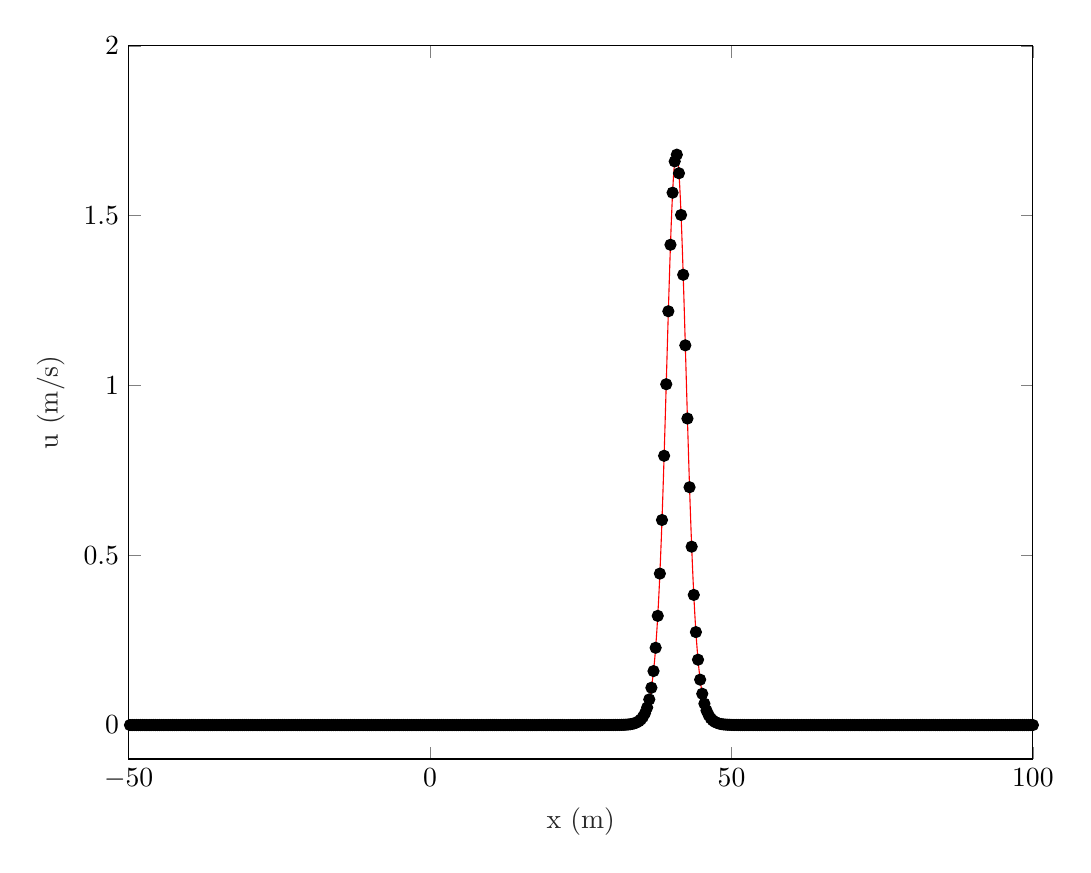
\begin{tikzpicture}

\begin{axis}[%
width=4.521in,
height=3.566in,
at={(0.758in,0.481in)},
scale only axis,
xmin=-50,
xmax=100,
xtick={-50,   0,  50, 100},
xlabel style={font=\color{white!15!black}},
xlabel={x (m)},
ymin=-0.1,
ymax=2,
ytick={  0, 0.5,   1, 1.5,   2},
ylabel style={font=\color{white!15!black}},
ylabel={u (m/s)},
axis background/.style={fill=white}
]
\addplot [color=red, forget plot]
  table[row sep=crcr]{%
-50.14064697609	0\\
-50.0234411626817	0\\
-49.9062353492733	0\\
-49.789029535865	0\\
-49.6718237224566	0\\
-49.5546179090483	0\\
-49.4374120956399	0\\
-49.3202062822316	0\\
-49.2030004688233	0\\
-49.0857946554149	0\\
-48.9685888420066	0\\
-48.8513830285982	0\\
-48.7341772151899	0\\
-48.6169714017815	0\\
-48.4997655883732	0\\
-48.3825597749648	0\\
-48.2653539615565	0\\
-48.1481481481481	0\\
-48.0309423347398	0\\
-47.9137365213315	0\\
-47.7965307079231	0\\
-47.6793248945148	0\\
-47.5621190811064	0\\
-47.4449132676981	0\\
-47.3277074542897	0\\
-47.2105016408814	0\\
-47.093295827473	0\\
-46.9760900140647	0\\
-46.8588842006564	0\\
-46.741678387248	0\\
-46.6244725738397	0\\
-46.5072667604313	0\\
-46.390060947023	0\\
-46.2728551336146	0\\
-46.1556493202063	0\\
-46.0384435067979	0\\
-45.9212376933896	0\\
-45.8040318799812	0\\
-45.6868260665729	0\\
-45.5696202531646	0\\
-45.4524144397562	0\\
-45.3352086263479	0\\
-45.2180028129395	0\\
-45.1007969995312	0\\
-44.9835911861228	0\\
-44.8663853727145	0\\
-44.7491795593061	0\\
-44.6319737458978	0\\
-44.5147679324894	0\\
-44.3975621190811	0\\
-44.2803563056728	0\\
-44.1631504922644	0\\
-44.0459446788561	0\\
-43.9287388654477	0\\
-43.8115330520394	0\\
-43.694327238631	0\\
-43.5771214252227	0\\
-43.4599156118143	0\\
-43.342709798406	0\\
-43.2255039849977	0\\
-43.1082981715893	0\\
-42.991092358181	0\\
-42.8738865447726	0\\
-42.7566807313643	0\\
-42.6394749179559	0\\
-42.5222691045476	0\\
-42.4050632911392	0\\
-42.2878574777309	0\\
-42.1706516643225	0\\
-42.0534458509142	0\\
-41.9362400375059	0\\
-41.8190342240975	0\\
-41.7018284106892	0\\
-41.5846225972808	0\\
-41.4674167838725	0\\
-41.3502109704641	0\\
-41.2330051570558	0\\
-41.1157993436474	0\\
-40.9985935302391	0\\
-40.8813877168308	0\\
-40.7641819034224	0\\
-40.6469760900141	0\\
-40.5297702766057	0\\
-40.4125644631974	0\\
-40.295358649789	0\\
-40.1781528363807	0\\
-40.0609470229723	0\\
-39.943741209564	0\\
-39.8265353961556	0\\
-39.7093295827473	0\\
-39.592123769339	0\\
-39.4749179559306	0\\
-39.3577121425223	0\\
-39.2405063291139	0\\
-39.1233005157056	0\\
-39.0060947022972	0\\
-38.8888888888889	0\\
-38.7716830754805	0\\
-38.6544772620722	0\\
-38.5372714486639	0\\
-38.4200656352555	0\\
-38.3028598218472	0\\
-38.1856540084388	0\\
-38.0684481950305	0\\
-37.9512423816221	0\\
-37.8340365682138	0\\
-37.7168307548054	0\\
-37.5996249413971	0\\
-37.4824191279887	0\\
-37.3652133145804	0\\
-37.2480075011721	0\\
-37.1308016877637	0\\
-37.0135958743554	0\\
-36.896390060947	0\\
-36.7791842475387	0\\
-36.6619784341303	0\\
-36.544772620722	0\\
-36.4275668073136	0\\
-36.3103609939053	0\\
-36.193155180497	0\\
-36.0759493670886	0\\
-35.9587435536803	0\\
-35.8415377402719	0\\
-35.7243319268636	0\\
-35.6071261134552	0\\
-35.4899203000469	0\\
-35.3727144866385	0\\
-35.2555086732302	0\\
-35.1383028598218	0\\
-35.0210970464135	0\\
-34.9038912330052	0\\
-34.7866854195968	0\\
-34.6694796061885	0\\
-34.5522737927801	0\\
-34.4350679793718	0\\
-34.3178621659634	0\\
-34.2006563525551	0\\
-34.0834505391467	0\\
-33.9662447257384	0\\
-33.8490389123301	0\\
-33.7318330989217	0\\
-33.6146272855134	0\\
-33.497421472105	0\\
-33.3802156586967	0\\
-33.2630098452883	0\\
-33.14580403188	0\\
-33.0285982184716	0\\
-32.9113924050633	0\\
-32.7941865916549	0\\
-32.6769807782466	0\\
-32.5597749648383	0\\
-32.4425691514299	0\\
-32.3253633380216	0\\
-32.2081575246132	0\\
-32.0909517112049	0\\
-31.9737458977965	0\\
-31.8565400843882	0\\
-31.7393342709798	0\\
-31.6221284575715	0\\
-31.5049226441632	0\\
-31.3877168307548	0\\
-31.2705110173465	0\\
-31.1533052039381	0\\
-31.0360993905298	0\\
-30.9188935771214	0\\
-30.8016877637131	0\\
-30.6844819503047	0\\
-30.5672761368964	0\\
-30.450070323488	0\\
-30.3328645100797	0\\
-30.2156586966714	0\\
-30.098452883263	0\\
-29.9812470698547	0\\
-29.8640412564463	0\\
-29.746835443038	0\\
-29.6296296296296	0\\
-29.5124238162213	0\\
-29.3952180028129	0\\
-29.2780121894046	0\\
-29.1608063759962	0\\
-29.0436005625879	0\\
-28.9263947491796	0\\
-28.8091889357712	0\\
-28.6919831223629	0\\
-28.5747773089545	0\\
-28.4575714955462	0\\
-28.3403656821378	0\\
-28.2231598687295	0\\
-28.1059540553211	0\\
-27.9887482419128	0\\
-27.8715424285045	0\\
-27.7543366150961	0\\
-27.6371308016878	0\\
-27.5199249882794	0\\
-27.4027191748711	0\\
-27.2855133614627	0\\
-27.1683075480544	0\\
-27.051101734646	0\\
-26.9338959212377	0\\
-26.8166901078293	0\\
-26.699484294421	0\\
-26.5822784810127	0\\
-26.4650726676043	0\\
-26.347866854196	0\\
-26.2306610407876	0\\
-26.1134552273793	0\\
-25.9962494139709	0\\
-25.8790436005626	0\\
-25.7618377871542	0\\
-25.6446319737459	0\\
-25.5274261603376	0\\
-25.4102203469292	0\\
-25.2930145335209	0\\
-25.1758087201125	0\\
-25.0586029067042	0\\
-24.9413970932958	0\\
-24.8241912798875	0\\
-24.7069854664791	0\\
-24.5897796530708	0\\
-24.4725738396624	0\\
-24.3553680262541	0\\
-24.2381622128458	0\\
-24.1209563994374	0\\
-24.0037505860291	0\\
-23.8865447726207	0\\
-23.7693389592124	0\\
-23.652133145804	0\\
-23.5349273323957	0\\
-23.4177215189873	0\\
-23.300515705579	0\\
-23.1833098921707	0\\
-23.0661040787623	0\\
-22.948898265354	0\\
-22.8316924519456	0\\
-22.7144866385373	0\\
-22.5972808251289	0\\
-22.4800750117206	0\\
-22.3628691983122	0\\
-22.2456633849039	0\\
-22.1284575714955	0\\
-22.0112517580872	0\\
-21.8940459446789	0\\
-21.7768401312705	0\\
-21.6596343178622	0\\
-21.5424285044538	0\\
-21.4252226910455	0\\
-21.3080168776371	0\\
-21.1908110642288	0\\
-21.0736052508204	0\\
-20.9563994374121	0\\
-20.8391936240038	0\\
-20.7219878105954	0\\
-20.6047819971871	0\\
-20.4875761837787	0\\
-20.3703703703704	0\\
-20.253164556962	0\\
-20.1359587435537	0\\
-20.0187529301453	0\\
-19.901547116737	0\\
-19.7843413033286	0\\
-19.6671354899203	0\\
-19.549929676512	0\\
-19.4327238631036	0\\
-19.3155180496953	0\\
-19.1983122362869	0\\
-19.0811064228786	0\\
-18.9639006094702	0\\
-18.8466947960619	0\\
-18.7294889826535	0\\
-18.6122831692452	0\\
-18.4950773558368	0\\
-18.3778715424285	0\\
-18.2606657290202	0\\
-18.1434599156118	0\\
-18.0262541022035	0\\
-17.9090482887951	0\\
-17.7918424753868	0\\
-17.6746366619784	0\\
-17.5574308485701	0\\
-17.4402250351617	0\\
-17.3230192217534	0\\
-17.2058134083451	0\\
-17.0886075949367	0\\
-16.9714017815284	0\\
-16.85419596812	0\\
-16.7369901547117	0\\
-16.6197843413033	0\\
-16.502578527895	0\\
-16.3853727144866	0\\
-16.2681669010783	0\\
-16.1509610876699	0\\
-16.0337552742616	0\\
-15.9165494608533	0\\
-15.7993436474449	0\\
-15.6821378340366	0\\
-15.5649320206282	0\\
-15.4477262072199	0\\
-15.3305203938115	0\\
-15.2133145804032	0\\
-15.0961087669948	0\\
-14.9789029535865	0\\
-14.8616971401782	0\\
-14.7444913267698	0\\
-14.6272855133615	0\\
-14.5100796999531	0\\
-14.3928738865448	0\\
-14.2756680731364	0\\
-14.1584622597281	0\\
-14.0412564463197	0\\
-13.9240506329114	0\\
-13.806844819503	0\\
-13.6896390060947	0\\
-13.5724331926864	0\\
-13.455227379278	0\\
-13.3380215658697	0\\
-13.2208157524613	0\\
-13.103609939053	0\\
-12.9864041256446	0\\
-12.8691983122363	0\\
-12.7519924988279	0\\
-12.6347866854196	0\\
-12.5175808720113	0\\
-12.4003750586029	0\\
-12.2831692451946	0\\
-12.1659634317862	0\\
-12.0487576183779	0\\
-11.9315518049695	0\\
-11.8143459915612	0\\
-11.6971401781528	0\\
-11.5799343647445	0\\
-11.4627285513361	0\\
-11.3455227379278	0\\
-11.2283169245195	0\\
-11.1111111111111	0\\
-10.9939052977028	0\\
-10.8766994842944	0\\
-10.7594936708861	0\\
-10.6422878574777	0\\
-10.5250820440694	0\\
-10.407876230661	0\\
-10.2906704172527	0\\
-10.1734646038444	0\\
-10.056258790436	0\\
-9.93905297702766	0\\
-9.82184716361932	0\\
-9.70464135021097	0\\
-9.58743553680262	0\\
-9.47022972339428	0\\
-9.35302390998594	0\\
-9.23581809657759	0\\
-9.11861228316924	0\\
-9.0014064697609	0\\
-8.88420065635255	0\\
-8.76699484294421	0\\
-8.64978902953587	0\\
-8.53258321612752	0\\
-8.41537740271917	0\\
-8.29817158931083	0\\
-8.18096577590249	0\\
-8.06375996249414	0\\
-7.94655414908579	0\\
-7.82934833567745	0\\
-7.7121425222691	0\\
-7.59493670886076	0\\
-7.47773089545242	0\\
-7.36052508204407	0\\
-7.24331926863572	0\\
-7.12611345522738	0\\
-7.00890764181904	0\\
-6.89170182841069	0\\
-6.77449601500234	0\\
-6.657290201594	0\\
-6.54008438818565	0\\
-6.42287857477731	0\\
-6.30567276136896	0\\
-6.18846694796062	0\\
-6.07126113455227	0\\
-5.95405532114393	0\\
-5.83684950773559	0\\
-5.71964369432724	0\\
-5.60243788091889	0\\
-5.48523206751055	0\\
-5.3680262541022	0\\
-5.25082044069386	0\\
-5.13361462728551	0\\
-5.01640881387717	0\\
-4.89920300046882	0\\
-4.78199718706048	0\\
-4.66479137365214	0\\
-4.54758556024379	0\\
-4.43037974683544	0\\
-4.31317393342709	0\\
-4.19596812001875	0\\
-4.07876230661041	0\\
-3.96155649320206	0\\
-3.84435067979372	0\\
-3.72714486638537	0\\
-3.60993905297703	0\\
-3.49273323956868	0\\
-3.37552742616034	0\\
-3.25832161275199	0\\
-3.14111579934364	0\\
-3.0239099859353	0\\
-2.90670417252696	0\\
-2.78949835911861	0\\
-2.67229254571027	0\\
-2.55508673230192	0\\
-2.43788091889358	0\\
-2.32067510548523	0\\
-2.20346929207689	0\\
-2.08626347866854	0\\
-1.96905766526019	0\\
-1.85185185185185	0\\
-1.73464603844351	0\\
-1.61744022503516	0\\
-1.50023441162681	0\\
-1.38302859821847	0\\
-1.26582278481013	0\\
-1.14861697140178	0\\
-1.03141115799344	0\\
-0.914205344585092	0\\
-0.796999531176745	0\\
-0.679793717768398	0\\
-0.562587904360058	0\\
-0.445382090951711	0\\
-0.328176277543363	0\\
-0.210970464135023	0\\
-0.0937646507266763	0\\
0.0234411626816708	0\\
0.140646976090011	0\\
0.257852789498358	0\\
0.375058602906705	0\\
0.492264416315052	0\\
0.609470229723392	0\\
0.726676043131739	0\\
0.843881856540087	0\\
0.961087669948427	0\\
1.07829348335677	0\\
1.19549929676512	0\\
1.31270511017347	0\\
1.42991092358181	0\\
1.54711673699016	0\\
1.6643225503985	0\\
1.78152836380684	0\\
1.89873417721519	0\\
2.01593999062354	0\\
2.13314580403188	0\\
2.25035161744022	0\\
2.36755743084857	0\\
2.48476324425692	0\\
2.60196905766526	0\\
2.71917487107361	0\\
2.83638068448195	0\\
2.95358649789029	0\\
3.07079231129864	0\\
3.18799812470699	0\\
3.30520393811533	0\\
3.42240975152367	0\\
3.53961556493202	0\\
3.65682137834037	0\\
3.77402719174871	0\\
3.89123300515705	0\\
4.0084388185654	0\\
4.12564463197375	0\\
4.24285044538209	0\\
4.36005625879044	0\\
4.47726207219878	0\\
4.59446788560712	0\\
4.71167369901547	0\\
4.82887951242382	0\\
4.94608532583216	0\\
5.0632911392405	0\\
5.18049695264885	0\\
5.2977027660572	0\\
5.41490857946554	0\\
5.53211439287389	0\\
5.64932020628223	0\\
5.76652601969058	0\\
5.88373183309892	0\\
6.00093764650727	0\\
6.11814345991561	0\\
6.23534927332395	0\\
6.3525550867323	0\\
6.46976090014065	0\\
6.58696671354899	0\\
6.70417252695734	0\\
6.82137834036568	0\\
6.93858415377403	9.06774273054312e-16\\
7.05578996718237	9.06774273054312e-16\\
7.17299578059072	9.06774273054312e-16\\
7.29020159399906	9.06774273054312e-16\\
7.4074074074074	9.06774273054312e-16\\
7.52461322081575	9.06774273054312e-16\\
7.6418190342241	9.06774273054312e-16\\
7.75902484763245	9.06774273054312e-16\\
7.87623066104079	1.81354854610862e-15\\
7.99343647444913	1.81354854610862e-15\\
8.11064228785748	1.81354854610862e-15\\
8.22784810126582	1.81354854610862e-15\\
8.34505391467417	2.72032281916294e-15\\
8.46225972808251	2.72032281916294e-15\\
8.57946554149086	2.72032281916294e-15\\
8.6966713548992	3.62709709221725e-15\\
8.81387716830755	3.62709709221725e-15\\
8.9310829817159	4.53387136527156e-15\\
9.04828879512424	5.44064563832587e-15\\
9.16549460853258	5.44064563832587e-15\\
9.28270042194093	6.34741991138018e-15\\
9.39990623534927	7.2541941844345e-15\\
9.51711204875762	9.06774273054312e-15\\
9.63431786216596	9.97451700359743e-15\\
9.75152367557431	1.08812912766517e-14\\
9.86872948898265	1.26948398227604e-14\\
9.985935302391	1.4508388368869e-14\\
10.1031411157993	1.63219369149776e-14\\
10.2203469292077	1.90422597341406e-14\\
10.337552742616	2.17625825533035e-14\\
10.4547585560244	2.44829053724664e-14\\
10.5719643694327	2.81100024646837e-14\\
10.6891701828411	3.17370995569009e-14\\
10.8063759962494	3.62709709221725e-14\\
10.9235818096578	4.0804842287444e-14\\
11.0407876230661	4.71522621988242e-14\\
11.1579934364744	5.34996821102044e-14\\
11.2751992498828	6.07538762946389e-14\\
11.3924050632911	6.89148447521277e-14\\
11.5096108766995	7.88893617557252e-14\\
11.6268166901078	8.97706530323769e-14\\
11.7440225035162	1.02465492855137e-13\\
11.8612283169245	1.16973881224006e-13\\
11.9784341303329	1.33295818138984e-13\\
12.0956399437412	1.5143130360007e-13\\
12.2128457571496	1.72287111880319e-13\\
12.3300515705579	1.96770017252786e-13\\
12.4472573839662	2.23973245444415e-13\\
12.5644631973746	2.54803570728262e-13\\
12.6816690107829	2.91074541650434e-13\\
12.7988748241913	3.30972609664824e-13\\
12.9160806375996	3.77218097590594e-13\\
13.033286451008	4.29811005427744e-13\\
13.1504922644163	4.89658107449328e-13\\
13.2676980778247	5.57666177928402e-13\\
13.384903891233	6.34741991138018e-13\\
13.5021097046413	7.23605869897341e-13\\
13.6193155180497	8.2425781420637e-13\\
13.736521331458	9.38511372611213e-13\\
13.8537271448664	1.06908686793103e-12\\
13.9709329582747	1.218704622985e-12\\
14.0881387716831	1.3873646377731e-12\\
14.2053445850914	1.58050755793367e-12\\
14.3225503984998	1.80085370628586e-12\\
14.4397562119081	2.05112340564885e-12\\
14.5569620253165	2.33675730166096e-12\\
14.6741678387248	2.66228926568746e-12\\
14.7913736521331	3.03225316909362e-12\\
14.9085794655415	3.45390320606387e-12\\
15.0257852789498	3.93449357078266e-12\\
15.1429910923582	4.48218523170746e-12\\
15.2601969057665	5.10604593156883e-12\\
15.3774027191749	5.81605018737036e-12\\
15.4946085325832	6.62579961320786e-12\\
15.6118143459916	7.54708227463104e-12\\
15.7290201593999	8.59712688282793e-12\\
15.8462259728083	9.79316214898657e-12\\
15.9634317862166	1.11560438813872e-11\\
16.0806375996249	1.27084414368562e-11\\
16.1978434130333	1.44766512693121e-11\\
16.3150492264416	1.64905969297657e-11\\
16.43225503985	1.87847358405931e-11\\
16.5494608532583	2.13980592955357e-11\\
16.6666666666667	2.4375906008246e-11\\
16.783872480075	2.77672417894691e-11\\
16.9010782934834	3.16301001926805e-11\\
17.0182841068917	3.60306757398131e-11\\
17.1354899203	4.10442306955304e-11\\
17.2526957337084	4.67541882929534e-11\\
17.3699015471167	5.3259386927845e-11\\
17.4871073605251	6.06695462872449e-11\\
17.6043131739334	6.91107079951074e-11\\
17.7215189873418	7.87261423865754e-11\\
17.8387248007501	8.96799756050715e-11\\
17.9559306141585	1.02157189602299e-10\\
18.0731364275668	1.16370876332425e-10\\
18.1903422409752	1.32562237752083e-10\\
18.3075480543835	1.51005119691735e-10\\
18.4247538677918	1.72015079598403e-10\\
18.5419596812002	1.95948479761398e-10\\
18.6591654946085	2.23210648280776e-10\\
18.7763713080169	2.54266760358614e-10\\
18.8935771214252	2.89643651847554e-10\\
19.0107829348336	3.29942514090634e-10\\
19.1279887482419	3.75847961664009e-10\\
19.2451945616503	4.28140727216778e-10\\
19.3624003750586	4.87708542762262e-10\\
19.4796061884669	5.55565181937735e-10\\
19.5968120018753	6.32862248069977e-10\\
19.7140178152836	7.20913657080643e-10\\
19.831223628692	8.21216493294545e-10\\
19.9484294421003	9.35474585570754e-10\\
20.0656352555087	1.06562933762788e-09\\
20.182841068917	1.2138923719179e-09\\
20.3000468823254	1.3827845209199e-09\\
20.4172526957337	1.57517481843383e-09\\
20.5344585091421	1.79433218571406e-09\\
20.6516643225504	2.04398255824855e-09\\
20.7688701359587	2.32836691931239e-09\\
20.8860759493671	2.65231837578095e-09\\
21.0032817627754	3.02134195426596e-09\\
21.1204875761838	3.44170890563984e-09\\
21.2376933895921	3.92056189085145e-09\\
21.3548992030005	4.46603920900146e-09\\
21.4721050164088	5.08741081348329e-09\\
21.5893108298172	5.79523427715812e-09\\
21.7065166432255	6.60153977430656e-09\\
21.8237224566338	7.52002866419446e-09\\
21.9409282700422	8.56630834560963e-09\\
22.0581340834505	9.7581597552724e-09\\
22.1753398968589	1.11158366033457e-08\\
22.2925457102672	1.26624108544331e-08\\
22.4097515236756	1.44241635472906e-08\\
22.5269573370839	1.64310327413173e-08\\
22.6441631504923	1.87171222169228e-08\\
22.7613689639006	2.13212818110619e-08\\
22.878574777309	2.42877648285823e-08\\
22.9957805907173	2.76669815716461e-08\\
23.1129864041256	3.151635578803e-08\\
23.230192217534	3.5901304894115e-08\\
23.3473980309423	4.0896341705628e-08\\
23.4646038443507	4.65863502690438e-08\\
23.581809657759	5.30680240055825e-08\\
23.6990154711674	6.04515087861918e-08\\
23.8162212845757	6.88622758738088e-08\\
23.9334270979841	7.84432546564492e-08\\
24.0506329113924	8.93572573616143e-08\\
24.1678387248007	1.01789751972017e-07\\
24.2850445382091	1.15952011452635e-07\\
24.4022503516174	1.32084700042954e-07\\
24.5194561650258	1.50461968249595e-07\\
24.6366619784341	1.71396111852519e-07\\
24.7538677918425	1.95242872907434e-07\\
24.8710736052508	2.2240749337084e-07\\
24.9882794186592	2.53351593436275e-07\\
25.1054852320675	2.88601021479201e-07\\
25.2226910454759	3.2875478759714e-07\\
25.3398968588842	3.74495244871209e-07\\
25.4571026722925	4.26599682475207e-07\\
25.5743084857009	4.85953536469996e-07\\
25.6915142991092	5.53565434548849e-07\\
25.8087201125176	6.30584339058476e-07\\
25.9259259259259	7.18319067128794e-07\\
26.0431317393343	8.18260536112787e-07\\
26.1603375527426	9.32107098406299e-07\\
26.277543366151	1.06179340089945e-06\\
26.3947491795593	1.20952326053126e-06\\
26.5119549929676	1.37780711769429e-06\\
26.629160806376	1.56950469452345e-06\\
26.7463666197843	1.78787358983615e-06\\
26.8635724331927	2.03662463996857e-06\\
26.980778246601	2.31998497313827e-06\\
27.0979840600094	2.64276984682245e-06\\
27.2151898734177	3.01046446917432e-06\\
27.3323956868261	3.42931721405818e-06\\
27.4496015002344	3.90644579388892e-06\\
27.5668073136428	4.44995821787938e-06\\
27.6840131270511	5.06909056369633e-06\\
27.8012189404594	5.77436392739224e-06\\
27.9184247538678	6.57776320528796e-06\\
28.0356305672761	7.49294074640665e-06\\
28.1528363806845	8.53544833888351e-06\\
28.2700421940928	9.72300147209892e-06\\
28.3872480075012	1.10757803598941e-05\\
28.5044538209095	1.26167728395292e-05\\
28.6216596343179	1.43721649746762e-05\\
28.7388654477262	1.63717859945929e-05\\
28.8560712611346	1.86496151297085e-05\\
28.9732770745429	2.12443589439223e-05\\
29.0904828879512	2.42001089776323e-05\\
29.2076887013596	2.7567090867513e-05\\
29.3248945147679	3.14025176564703e-05\\
29.4421003281763	3.57715617881077e-05\\
29.5593061415846	4.07484622794739e-05\\
29.676511954993	4.64177858754163e-05\\
29.7937177684013	5.28758635689993e-05\\
29.9109235818097	6.02324268779463e-05\\
30.028129395218	6.8612471626214e-05\\
30.1453352086263	7.81583808349547e-05\\
30.2625410220347	8.90323427240722e-05\\
30.379746835443	0.000101419104795608\\
30.4969526488514	0.00011552911067516\\
30.6141584622597	0.000131602072815669\\
30.7313642756681	0.000149911041553117\\
30.8485700890764	0.00017076703935599\\
30.9657759024848	0.000194524338611991\\
31.0829817158931	0.000221586472133703\\
31.2001875293015	0.000252413077847617\\
31.3173933427098	0.000287527693114307\\
31.4345991561181	0.000327526630003336\\
31.5518049695265	0.000373089080882208\\
31.6690107829348	0.000424988624155939\\
31.7862165963432	0.000484106323209475\\
31.9034224097515	0.000551445637959232\\
32.0206282231599	0.000628149398278317\\
32.1378340365682	0.000715519122346805\\
32.2550398499766	0.000815037001262058\\
32.3722456633849	0.000928390914450008\\
32.4894514767932	0.00105750288927762\\
32.6066572902016	0.00120456147328252\\
32.7238631036099	0.00137205854946016\\
32.8410689170183	0.00156283119467619\\
32.9582747304266	0.00178010925943831\\
33.075480543835	0.00202756943468269\\
33.1926863572433	0.00230939666879157\\
33.3098921706517	0.00263035390653889\\
33.42709798406	0.002995861241836\\
33.5443037974684	0.00341208570866381\\
33.6615096108767	0.00388604307979318\\
33.778715424285	0.00442571320104597\\
33.8959212376934	0.00504017055957566\\
34.0131270511017	0.00573973196690971\\
34.1303328645101	0.00653612342967975\\
34.2475386779184	0.00744266847969811\\
34.3647444913268	0.00847450043594509\\
34.4819503047351	0.00964880126703259\\
34.5991561181435	0.0109850699041282\\
34.7163619315518	0.0125054230078522\\
34.8335677449601	0.0142349312998318\\
34.9507735583685	0.0162019946063359\\
35.0679793717768	0.0184387586954479\\
35.1851851851852	0.0209815767790725\\
35.3023909985935	0.0238715181430804\\
35.4195968120019	0.0271549256952327\\
35.5368026254102	0.0308840231960466\\
35.6540084388186	0.0351175714574539\\
35.7712142522269	0.0399215707299474\\
35.8884200656353	0.0453700036984107\\
36.0056258790436	0.0515456097915298\\
36.122831692452	0.0585406766774211\\
36.2400375058603	0.066457828647872\\
36.3572433192686	0.0754107838569794\\
36.474449132677	0.0855250428609074\\
36.5916549460853	0.0969384594317847\\
36.7088607594937	0.109801631109072\\
36.826066572902	0.124278031483017\\
36.9432723863104	0.140543789101873\\
37.0604781997187	0.158786999845292\\
37.177684013127	0.179206441798467\\
37.2948898265354	0.202009545932535\\
37.4120956399437	0.22740946487397\\
37.5293014533521	0.255621079244283\\
37.6465072667604	0.28685579086935\\
37.7637130801688	0.321314979698232\\
37.8809188935771	0.359182051898698\\
37.9981247069855	0.400613085141572\\
38.1153305203938	0.445726186646318\\
38.2325363338022	0.494589819921988\\
38.3497421472105	0.547210521986804\\
38.4669479606189	0.603520612124091\\
38.5841537740272	0.663366666180676\\
38.7013595874355	0.72649967006103\\
38.8185654008439	0.792567840764187\\
38.9357712142522	0.861113081704344\\
39.0529770276606	0.931571897213825\\
39.1701828410689	1.00328132053016\\
39.2873886544773	1.07549002388592\\
39.4045944678856	1.14737431737289\\
39.5218002812939	1.21805826602\\
39.6390060947023	1.28663673549676\\
39.7562119081106	1.35219988723851\\
39.873417721519	1.41385753620772\\
39.9906235349273	1.47076187989757\\
40.1078293483357	1.52212738904434\\
40.225035161744	1.56724706833021\\
40.3422409751524	1.60550477611835\\
40.4594467885607	1.63638375643018\\
40.5766526019691	1.65947191363387\\
40.6938584153774	1.67446460119774\\
40.8110642287858	1.68116577729349\\
40.9282700421941	1.679488304982\\
41.0454758556024	1.66945396779611\\
41.1626816690108	1.65119347281564\\
41.2798874824191	1.62494637213412\\
41.3970932958275	1.59106050313487\\
41.5142991092358	1.54999028046363\\
41.6315049226442	1.50229301432615\\
41.7487107360525	1.44862241540816\\
41.8659165494608	1.38971859296451\\
41.9831223628692	1.32639415235617\\
42.1003281762775	1.25951641763248\\
42.2175339896859	1.18998628483471\\
42.3347398030942	1.11871467683508\\
42.4519456165026	1.04659794179064\\
42.5691514299109	0.974493748905007\\
42.6863572433193	0.903199049253638\\
42.8035630567276	0.833431484522666\\
42.920768870136	0.765815277425135\\
43.0379746835443	0.7008721862066\\
43.1551804969527	0.639017626126788\\
43.272386310361	0.580561623139842\\
43.3895921237693	0.525713922101334\\
43.5067979371777	0.474592352456931\\
43.624003750586	0.427233462682169\\
43.7412095639944	0.383604455121435\\
43.8584153774027	0.343615557468145\\
43.9756211908111	0.307132123716976\\
44.0928270042194	0.273985935762325\\
44.2100328176277	0.243985352652912\\
44.3272386310361	0.216924111204356\\
44.4444444444444	0.192588710024351\\
44.5616502578528	0.170764405960209\\
44.6788560712611	0.151239918856142\\
44.7960618846695	0.133810981268217\\
44.9132676980778	0.118282889593725\\
45.0304735114862	0.104472217262382\\
45.1476793248945	0.0922078440667746\\
45.2648851383029	0.0813314424334248\\
45.3820909517112	0.0716975446069546\\
45.4992967651196	0.0631732966348332\\
45.6165025785279	0.0556379872581005\\
45.7337083919362	0.0489824233049075\\
45.8509142053446	0.0431082084757877\\
45.9681200187529	0.0379269697156838\\
46.0853258321613	0.0333595646920224\\
46.2025316455696	0.0293352951160212\\
46.319737458978	0.0257911435615636\\
46.4369432723863	0.0226710458282338\\
46.5541490857947	0.0199252065352604\\
46.671354899203	0.0175094623067961\\
46.7885607126113	0.0153846944228922\\
46.9057665260197	0.01351629099686\\
47.022972339428	0.0118736574557193\\
47.1401781528364	0.0104297732277176\\
47.2573839662447	0.00916079198268795\\
47.3745897796531	0.00804568244945439\\
47.4917955930614	0.00706590668768253\\
47.6090014064698	0.00620513267114321\\
47.7262072198781	0.00544897810760407\\
47.8434130332865	0.00478478254886827\\
47.9606188466948	0.00420140501100139\\
48.0778246601031	0.00368904451347711\\
48.1950304735115	0.00323908114488455\\
48.3122362869198	0.00284393546359155\\
48.4294421003282	0.00249694423831388\\
48.5466479137365	0.00219225072204547\\
48.6638537271449	0.00192470783064548\\
48.7810595405532	0.00168979276311278\\
48.8982653539616	0.00148353175357757\\
49.0154711673699	0.00130243378515719\\
49.1326769807782	0.00114343222330498\\
49.2498827941866	0.00100383344171454\\
49.3670886075949	0.000881271617858047\\
49.4842944210033	0.000773668968633056\\
49.6015002344116	0.000679200780229493\\
49.71870604782	0.000596264660961034\\
49.8359118612283	0.000523453512314844\\
49.9531176746367	0.000459531772598186\\
50.070323488045	0.000403414540043558\\
50.1875293014534	0.000354149228735224\\
50.3047351148617	0.000310899451916122\\
50.42194092827	0.000272930863634315\\
50.5391467416784	0.000239598721858688\\
50.6563525550867	0.000210336964605091\\
50.7735583684951	0.000184648615646573\\
50.8907641819034	0.000162097358477567\\
51.0079699953118	0.000142300136678561\\
51.1251758087201	0.00012492065592359\\
51.2423816221285	0.000109663678018346\\
51.3595874355368	9.62700105928315e-05\\
51.4767932489451	8.45121077680922e-05\\
51.5939990623535	7.41902074147901e-05\\
51.7112048757618	6.51289396111296e-05\\
51.8284106891702	5.71743489067714e-05\\
51.9456165025785	5.01912799321048e-05\\
52.0628223159869	4.40610820660213e-05\\
52.1800281293952	3.86795942493338e-05\\
52.2972339428036	3.39553757725054e-05\\
52.4144397562119	2.98081530316197e-05\\
52.5316455696203	2.61674559040006e-05\\
52.6488513830286	2.29714206021477e-05\\
52.7660571964369	2.01657386928834e-05\\
52.8832630098453	1.77027344350346e-05\\
53.0004688232536	1.55405547838175e-05\\
53.117674636662	1.36424582934657e-05\\
53.2348804500703	1.19761908607231e-05\\
53.3520862634787	1.05134376963164e-05\\
53.469292076887	9.22934221546216e-06\\
53.5864978902954	8.10208369414741e-06\\
53.7037037037037	7.11250648867616e-06\\
53.820909517112	6.24379454632367e-06\\
53.9381153305204	5.48118566353429e-06\\
54.0553211439287	4.8117206426874e-06\\
54.1725269573371	4.22402307924488e-06\\
54.2897327707454	3.70810605334463e-06\\
54.4069385841538	3.25520241656744e-06\\
54.5241443975621	2.85761582161884e-06\\
54.6413502109705	2.50858993510192e-06\\
54.7585560243788	2.20219362674614e-06\\
54.8757618377872	1.93322018280707e-06\\
54.9929676511955	1.69709882847348e-06\\
55.1101734646038	1.48981705448983e-06\\
55.2273792780122	1.30785243362502e-06\\
55.3445850914205	1.1481127608755e-06\\
55.4617909048289	1.00788350952327e-06\\
55.5789967182372	8.8478170126165e-07\\
55.6962025316456	7.76715410563015e-07\\
55.8134083450539	6.81848216860387e-07\\
55.9306141584623	5.98567998817575e-07\\
56.0478199718706	5.25459535691138e-07\\
56.165025785279	4.61280461943597e-07\\
56.2822315986873	4.04940150737552e-07\\
56.3994374120956	3.55481184910186e-07\\
56.516643225504	3.1206308400216e-07\\
56.6338490389123	2.73948025283137e-07\\
56.7510548523207	2.40488298529712e-07\\
56.868260665729	2.11115308667032e-07\\
56.9854664791374	1.8532990320762e-07\\
57.1026722925457	1.6269390161951e-07\\
57.2198781059541	1.4282263756123e-07\\
57.3370839193624	1.25378428293497e-07\\
57.4542897327707	1.10064836611609e-07\\
57.5714955461791	9.66216314474252e-08\\
57.6887013595874	8.48203655312391e-08\\
57.8059071729958	7.44604934911119e-08\\
57.9231129864041	6.53659660087041e-08\\
58.0403187998125	5.7382233837078e-08\\
58.1575246132208	5.03736272230475e-08\\
58.2747304266292	4.42210449929443e-08\\
58.3919362400375	3.88199319926007e-08\\
58.5091420534459	3.40785054368727e-08\\
58.6263478668542	2.99161916307922e-08\\
58.7435536802625	2.62622594607382e-08\\
58.8607594936709	2.3054613477879e-08\\
58.9779653070792	2.02387474806614e-08\\
59.0951711204876	1.77668073635993e-08\\
59.2123769338959	1.55967877152675e-08\\
59.3295827473043	1.36918118395297e-08\\
59.4467885607126	1.20195088016119e-08\\
59.563994374121	1.05514575754739e-08\\
59.6812001875293	9.26271370763817e-09\\
59.7984060009376	8.13137587908768e-09\\
59.915611814346	7.13821775491085e-09\\
60.0328176277543	6.26636335911186e-09\\
60.1500234411627	5.500996000069e-09\\
60.267229254571	4.82910981438386e-09\\
60.3844350679794	4.23928760718441e-09\\
60.5016408813877	3.72150498888202e-09\\
60.6188466947961	3.26696443547954e-09\\
60.7360525082044	2.86794113694481e-09\\
60.8532583216128	2.51765332848966e-09\\
60.9704641350211	2.21014985056003e-09\\
61.0876699484294	1.94020405624603e-09\\
61.2048757618378	1.70322948127456e-09\\
61.3220815752461	1.49519914109899e-09\\
61.4392873886545	1.3125766160544e-09\\
61.5564932020628	1.15225983135267e-09\\
61.6736990154712	1.01152393030327e-09\\
61.7909048288795	8.87977749148169e-10\\
61.9081106422879	7.79521198670962e-10\\
62.0253164556962	6.84310806774532e-10\\
62.1425222691045	6.00729794930024e-10\\
62.2597280825129	5.27357247851561e-10\\
62.3769338959212	4.62946350913695e-10\\
62.4941397093296	4.06402627568847e-10\\
62.6113455227379	3.56764897087581e-10\\
62.7285513361463	3.13189859395956e-10\\
62.8457571495546	2.7493758668716e-10\\
62.962962962963	2.41357015033139e-10\\
63.0801687763713	2.11877783416144e-10\\
63.1973745897797	1.85999352437447e-10\\
63.314580403188	1.63281936574617e-10\\
63.4317862165964	1.4333834321306e-10\\
63.5489920300047	1.25831252323201e-10\\
63.666197843413	1.10462335169203e-10\\
63.7834036568214	9.69704407604281e-11\\
63.9006094702297	8.51270619800658e-11\\
64.0178152836381	7.4729081390952e-11\\
64.1350210970464	6.56023983326603e-11\\
64.2522269104548	5.75892340816794e-11\\
64.3694327238631	5.05553860455971e-11\\
64.4866385372714	4.43811600203702e-11\\
64.6038443506798	3.89604634160516e-11\\
64.7210501640881	3.42017120310625e-11\\
64.8382559774965	3.00242029551013e-11\\
64.9554617909048	2.63572077948697e-11\\
65.0726676043132	2.31381591255269e-11\\
65.1898734177215	2.03117437164166e-11\\
65.3070792311299	1.783080930534e-11\\
65.4242850445382	1.56527375014635e-11\\
65.5414908579466	1.3741257333865e-11\\
65.6586966713549	1.20628181544415e-11\\
65.7759024847633	1.05893099607283e-11\\
65.8931082981716	9.29624984735281e-12\\
66.0103141115799	8.16096845748881e-12\\
66.1275199249883	7.16442353140212e-12\\
66.2447257383966	6.28938635790471e-12\\
66.361931551805	5.52044177435465e-12\\
66.4791373652133	4.8467084894753e-12\\
66.5963431786217	4.25458488917083e-12\\
66.71354899203	3.73500323071071e-12\\
66.8307548054383	3.27889577136439e-12\\
66.9479606188467	2.87810154267439e-12\\
67.065166432255	2.52717989900237e-12\\
67.1823722456634	2.21796987189085e-12\\
67.2995780590717	1.94684436424761e-12\\
67.4167838724801	1.70926950470738e-12\\
67.5339896858884	1.50071142190489e-12\\
67.6511954992968	1.31754301874792e-12\\
67.7684013127051	1.15613719814425e-12\\
67.8856071261135	1.01558718582083e-12\\
68.0028129395218	8.91359110412389e-13\\
68.1200187529302	7.82546197645871e-13\\
68.2372245663385	6.86428124702114e-13\\
68.3544303797468	6.03004891581117e-13\\
68.4716361931552	5.29556175463718e-13\\
68.5888420065635	4.64268427803808e-13\\
68.7060478199719	4.0804842287444e-13\\
68.8232536333802	3.58175837856453e-13\\
68.9404594467886	3.14650672749846e-13\\
69.0576652601969	2.75659379008511e-13\\
69.1748710736052	2.42108730905501e-13\\
69.2920768870136	2.13091954167763e-13\\
69.4092827004219	1.86795500249188e-13\\
69.5264885138303	1.6412614342283e-13\\
69.6436943272386	1.44177109415636e-13\\
69.760900140647	1.26041623954549e-13\\
69.8781059540553	1.10626461312626e-13\\
69.9953117674637	9.70248472168114e-14\\
70.112517580872	8.52367816671053e-14\\
70.2297233942804	7.52622646635079e-14\\
70.3469292076887	6.61945219329648e-14\\
70.4641350210971	5.8033553475476e-14\\
70.5813408345054	5.07793592910415e-14\\
70.6985466479137	4.44319393796613e-14\\
70.8157524613221	3.89912937413354e-14\\
70.9329582747304	3.44574223760639e-14\\
71.0501640881388	2.99235510107923e-14\\
71.1673699015471	2.6296453918575e-14\\
71.2845757149555	2.35761310994121e-14\\
71.4017815283638	1.99490340071949e-14\\
71.5189873417721	1.81354854610862e-14\\
71.6361931551805	1.54151626419233e-14\\
71.7533989685888	1.36016140958147e-14\\
71.8706047819972	1.17880655497061e-14\\
71.9878105954055	1.08812912766517e-14\\
72.1050164088139	9.06774273054312e-15\\
72.2222222222222	8.16096845748881e-15\\
72.3394280356306	7.2541941844345e-15\\
72.4566338490389	6.34741991138018e-15\\
72.5738396624473	5.44064563832587e-15\\
72.6910454758556	4.53387136527156e-15\\
72.8082512892639	4.53387136527156e-15\\
72.9254571026723	3.62709709221725e-15\\
73.0426629160806	3.62709709221725e-15\\
73.159868729489	2.72032281916294e-15\\
73.2770745428973	2.72032281916294e-15\\
73.3942803563057	1.81354854610862e-15\\
73.511486169714	1.81354854610862e-15\\
73.6286919831224	1.81354854610862e-15\\
73.7458977965307	1.81354854610862e-15\\
73.8631036099391	9.06774273054312e-16\\
73.9803094233474	9.06774273054312e-16\\
74.0975152367557	9.06774273054312e-16\\
74.2147210501641	9.06774273054312e-16\\
74.3319268635724	9.06774273054312e-16\\
74.4491326769808	9.06774273054312e-16\\
74.5663384903891	9.06774273054312e-16\\
74.6835443037975	9.06774273054312e-16\\
74.8007501172058	9.06774273054312e-16\\
74.9179559306142	0\\
75.0351617440225	0\\
75.1523675574308	0\\
75.2695733708392	0\\
75.3867791842475	0\\
75.5039849976559	0\\
75.6211908110642	0\\
75.7383966244726	0\\
75.8556024378809	0\\
75.9728082512893	0\\
76.0900140646976	0\\
76.207219878106	0\\
76.3244256915143	0\\
76.4416315049226	0\\
76.558837318331	0\\
76.6760431317393	0\\
76.7932489451477	0\\
76.910454758556	0\\
77.0276605719644	0\\
77.1448663853727	0\\
77.2620721987811	0\\
77.3792780121894	0\\
77.4964838255977	0\\
77.6136896390061	0\\
77.7308954524144	0\\
77.8481012658228	0\\
77.9653070792311	0\\
78.0825128926395	0\\
78.1997187060478	0\\
78.3169245194562	0\\
78.4341303328645	0\\
78.5513361462729	0\\
78.6685419596812	0\\
78.7857477730896	0\\
78.9029535864979	0\\
79.0201593999062	0\\
79.1373652133146	0\\
79.2545710267229	0\\
79.3717768401313	0\\
79.4889826535396	0\\
79.606188466948	0\\
79.7233942803563	0\\
79.8406000937647	0\\
79.957805907173	0\\
80.0750117205813	0\\
80.1922175339897	0\\
80.309423347398	0\\
80.4266291608064	0\\
80.5438349742147	0\\
80.6610407876231	0\\
80.7782466010314	0\\
80.8954524144397	0\\
81.0126582278481	0\\
81.1298640412564	0\\
81.2470698546648	0\\
81.3642756680731	0\\
81.4814814814815	0\\
81.5986872948898	0\\
81.7158931082982	0\\
81.8330989217065	0\\
81.9503047351149	0\\
82.0675105485232	0\\
82.1847163619315	0\\
82.3019221753399	0\\
82.4191279887482	0\\
82.5363338021566	0\\
82.6535396155649	0\\
82.7707454289733	0\\
82.8879512423816	0\\
83.00515705579	0\\
83.1223628691983	0\\
83.2395686826067	0\\
83.356774496015	0\\
83.4739803094234	0\\
83.5911861228317	0\\
83.70839193624	0\\
83.8255977496484	0\\
83.9428035630567	0\\
84.0600093764651	0\\
84.1772151898734	0\\
84.2944210032818	0\\
84.4116268166901	0\\
84.5288326300985	0\\
84.6460384435068	0\\
84.7632442569152	0\\
84.8804500703235	0\\
84.9976558837318	0\\
85.1148616971402	0\\
85.2320675105485	0\\
85.3492733239569	0\\
85.4664791373652	0\\
85.5836849507735	0\\
85.7008907641819	0\\
85.8180965775902	0\\
85.9353023909986	0\\
86.0525082044069	0\\
86.1697140178153	0\\
86.2869198312236	0\\
86.404125644632	0\\
86.5213314580403	0\\
86.6385372714487	0\\
86.755743084857	0\\
86.8729488982653	0\\
86.9901547116737	0\\
87.107360525082	0\\
87.2245663384904	0\\
87.3417721518987	0\\
87.4589779653071	0\\
87.5761837787154	0\\
87.6933895921238	0\\
87.8105954055321	0\\
87.9278012189405	0\\
88.0450070323488	0\\
88.1622128457572	0\\
88.2794186591655	0\\
88.3966244725738	0\\
88.5138302859822	0\\
88.6310360993905	0\\
88.7482419127989	0\\
88.8654477262072	0\\
88.9826535396156	0\\
89.0998593530239	0\\
89.2170651664323	0\\
89.3342709798406	0\\
89.451476793249	0\\
89.5686826066573	0\\
89.6858884200656	0\\
89.803094233474	0\\
89.9203000468823	0\\
90.0375058602907	0\\
90.154711673699	0\\
90.2719174871074	0\\
90.3891233005157	0\\
90.506329113924	0\\
90.6235349273324	0\\
90.7407407407407	0\\
90.8579465541491	0\\
90.9751523675574	0\\
91.0923581809658	0\\
91.2095639943741	0\\
91.3267698077825	0\\
91.4439756211908	0\\
91.5611814345991	0\\
91.6783872480075	0\\
91.7955930614158	0\\
91.9127988748242	0\\
92.0300046882325	0\\
92.1472105016409	0\\
92.2644163150492	0\\
92.3816221284576	0\\
92.4988279418659	0\\
92.6160337552743	0\\
92.7332395686826	0\\
92.850445382091	0\\
92.9676511954993	0\\
93.0848570089076	0\\
93.202062822316	0\\
93.3192686357243	0\\
93.4364744491327	0\\
93.553680262541	0\\
93.6708860759494	0\\
93.7880918893577	0\\
93.9052977027661	0\\
94.0225035161744	0\\
94.1397093295828	0\\
94.2569151429911	0\\
94.3741209563995	0\\
94.4913267698078	0\\
94.6085325832161	0\\
94.7257383966245	0\\
94.8429442100328	0\\
94.9601500234412	0\\
95.0773558368495	0\\
95.1945616502579	0\\
95.3117674636662	0\\
95.4289732770745	0\\
95.5461790904829	0\\
95.6633849038912	0\\
95.7805907172996	0\\
95.8977965307079	0\\
96.0150023441163	0\\
96.1322081575246	0\\
96.2494139709329	0\\
96.3666197843413	0\\
96.4838255977496	0\\
96.601031411158	0\\
96.7182372245663	0\\
96.8354430379747	0\\
96.952648851383	0\\
97.0698546647914	0\\
97.1870604781997	0\\
97.3042662916081	0\\
97.4214721050164	0\\
97.5386779184248	0\\
97.6558837318331	0\\
97.7730895452414	0\\
97.8902953586498	0\\
98.0075011720581	0\\
98.1247069854665	0\\
98.2419127988748	0\\
98.3591186122832	0\\
98.4763244256915	0\\
98.5935302390999	0\\
98.7107360525082	0\\
98.8279418659166	0\\
98.9451476793249	0\\
99.0623534927333	0\\
99.1795593061416	0\\
99.2967651195499	0\\
99.4139709329583	0\\
99.5311767463666	0\\
99.648382559775	0\\
99.7655883731833	0\\
99.8827941865917	0\\
100	0\\
100.117205813408	0\\
};
\addplot [color=black, draw=none, mark=*, mark options={solid, black}, forget plot]
  table[row sep=crcr]{%
-50.14064697609	0\\
-49.789029535865	1.33338460333001e-10\\
-49.4374120956399	2.97683161924035e-10\\
-49.0857946554149	4.84780876856103e-10\\
-48.7341772151899	7.08589649035313e-10\\
-48.3825597749648	9.85435419619768e-10\\
-48.0309423347398	1.33507012041878e-09\\
-47.6793248945148	1.78186157475441e-09\\
-47.3277074542897	2.35621823842691e-09\\
-46.9760900140647	3.09630325640272e-09\\
-46.6244725738397	4.05011367185402e-09\\
-46.2728551336146	5.27799556116659e-09\\
-45.9212376933896	6.8556905156935e-09\\
-45.5696202531646	8.87801304854708e-09\\
-45.2180028129395	1.14632561792719e-08\\
-44.8663853727145	1.47584537692207e-08\\
-44.5147679324894	1.89456095541628e-08\\
-44.1631504922644	2.42490356714833e-08\\
-43.8115330520394	3.09438949927862e-08\\
-43.4599156118143	3.93660717777273e-08\\
-43.1082981715893	4.99234511427992e-08\\
-42.7566807313643	6.31086536333555e-08\\
-42.4050632911392	7.95132005682686e-08\\
-42.0534458509142	9.98430389391673e-08\\
-41.7018284106892	1.24935202213762e-07\\
-41.3502109704641	1.55775281964175e-07\\
-40.9985935302391	1.93515178161188e-07\\
-40.6469760900141	2.39490396952283e-07\\
-40.295358649789	2.95235878761624e-07\\
-39.943741209564	3.62499070013603e-07\\
-39.592123769339	4.43248560216823e-07\\
-39.2405063291139	5.39676269621797e-07\\
-38.8888888888889	6.54190759327367e-07\\
-38.5372714486639	7.89398858378004e-07\\
-38.1856540084388	9.48072452121548e-07\\
-37.8340365682138	1.13309701325416e-06\\
-37.4824191279887	1.34739832978536e-06\\
-37.1308016877637	1.59384397112592e-06\\
-36.7791842475387	1.87511638241896e-06\\
-36.4275668073136	2.19355524509088e-06\\
-36.0759493670886	2.5509679456184e-06\\
-35.7243319268636	2.9484087558802e-06\\
-35.3727144866385	3.385929730142e-06\\
-35.0210970464135	3.86230941634693e-06\\
-34.6694796061885	4.37476929970734e-06\\
-34.3178621659634	4.91869233540498e-06\\
-33.9662447257384	5.48736290383691e-06\\
-33.6146272855134	6.07175279017139e-06\\
-33.2630098452883	6.66038287283543e-06\\
-32.9113924050633	7.23929472843268e-06\\
-32.5597749648383	7.7921694811506e-06\\
-32.2081575246132	8.30063221076705e-06\\
-31.8565400843882	8.74477803881816e-06\\
-31.5049226441632	9.10394964867292e-06\\
-31.1533052039381	9.35778440107857e-06\\
-30.8016877637131	9.48753156271414e-06\\
-30.450070323488	9.47761270555105e-06\\
-30.098452883263	9.31738941513813e-06\\
-29.746835443038	9.00300502242732e-06\\
-29.3952180028129	8.53921976175087e-06\\
-29.0436005625879	7.94103299954517e-06\\
-28.6919831223629	7.2348936186109e-06\\
-28.3403656821378	6.45925780893397e-06\\
-27.9887482419128	5.66424312787201e-06\\
-27.6371308016878	4.91013963788634e-06\\
-27.2855133614627	4.26458294370341e-06\\
-26.9338959212377	3.79827679022336e-06\\
-26.5822784810127	3.57927856404587e-06\\
-26.2306610407876	3.6660373891874e-06\\
-25.8790436005626	4.09953103192624e-06\\
-25.5274261603376	4.89521633880276e-06\\
-25.1758087201125	6.03552120980725e-06\\
-24.8241912798875	7.46400492920237e-06\\
-24.4725738396624	9.08233086174378e-06\\
-24.1209563994374	1.07512386061004e-05\\
-23.7693389592124	1.22965473827971e-05\\
-23.4177215189873	1.35208711263208e-05\\
-23.0661040787623	1.42211551585144e-05\\
-22.7144866385373	1.42113457850028e-05\\
-22.3628691983122	1.33486669822111e-05\\
-22.0112517580872	1.15606662919009e-05\\
-21.6596343178622	8.86968860553053e-06\\
-21.3080168776371	5.41037826320181e-06\\
-20.9563994374121	1.43578881469432e-06\\
-20.6047819971871	-2.69188807627503e-06\\
-20.253164556962	-6.5286387687305e-06\\
-19.901547116737	-9.59443239839944e-06\\
-19.549929676512	-1.14349347720072e-05\\
-19.1983122362869	-1.16929742521157e-05\\
-18.8466947960619	-1.01804136466077e-05\\
-18.4950773558368	-6.93745537747186e-06\\
-18.1434599156118	-2.2664873880967e-06\\
-17.7918424753868	3.27238205904421e-06\\
-17.4402250351617	8.91225734259901e-06\\
-17.0886075949367	1.37780552277431e-05\\
-16.7369901547117	1.70244119861747e-05\\
-16.3853727144866	1.79938835555958e-05\\
-16.0337552742616	1.63674358908694e-05\\
-15.6821378340366	1.22730124369411e-05\\
-15.3305203938115	6.31954067837748e-06\\
-14.9789029535865	-4.66459827786461e-07\\
-14.6272855133615	-6.8071375427286e-06\\
-14.2756680731364	-1.14228685091052e-05\\
-13.9240506329114	-1.33197074966286e-05\\
-13.5724331926864	-1.20487428815103e-05\\
-13.2208157524613	-7.86586971660065e-06\\
-12.8691983122363	-1.72889784779393e-06\\
-12.5175808720113	4.89042874755737e-06\\
-12.1659634317862	1.03570033485027e-05\\
-11.8143459915612	1.33053995705225e-05\\
-11.4627285513361	1.30348254866004e-05\\
-11.1111111111111	9.73855177098587e-06\\
-10.7594936708861	4.47093027824887e-06\\
-10.407876230661	-1.16108560149178e-06\\
-10.056258790436	-5.50247978588365e-06\\
-9.70464135021097	-7.38542093395537e-06\\
-9.35302390998594	-6.50065063271628e-06\\
-9.0014064697609	-3.45877861838807e-06\\
-8.64978902953587	4.88860884639841e-07\\
-8.29817158931083	3.95180248194184e-06\\
-7.94655414908579	5.90999997420874e-06\\
-7.59493670886076	6.01565401880961e-06\\
-7.24331926863572	4.58507948615589e-06\\
-6.89170182841069	2.34086155445585e-06\\
-6.54008438818565	8.3484099356668e-08\\
-6.18846694796062	-1.54164800891977e-06\\
-5.83684950773559	-2.13994513579281e-06\\
-5.48523206751055	-1.60542164304645e-06\\
-5.13361462728551	-1.75206193087525e-07\\
-4.78199718706048	1.55557340646471e-06\\
-4.43037974683544	2.80792776510332e-06\\
-4.07876230661041	3.01060369527548e-06\\
-3.72714486638537	2.16761931763061e-06\\
-3.37552742616034	8.6323669531977e-07\\
-3.0239099859353	-1.51322496199073e-07\\
-2.67229254571027	-4.42385460057819e-07\\
-2.32067510548523	-6.76488720261088e-08\\
-1.96905766526019	6.19124820139388e-07\\
-1.61744022503516	1.25945939480123e-06\\
-1.26582278481013	1.59859610850754e-06\\
-0.914205344585092	1.43978048622033e-06\\
-0.562587904360058	7.65155586848382e-07\\
-0.210970464135023	1.5111471142476e-07\\
0.140646976090011	5.06466123961307e-07\\
0.492264416315052	9.72559718048777e-07\\
0.843881856540087	-3.66260039581897e-07\\
1.19549929676512	2.52593316886242e-06\\
1.54711673699016	-8.97240389414172e-07\\
1.89873417721519	2.11841862850306e-06\\
2.25035161744022	2.89815507368055e-06\\
2.60196905766526	-2.92939859289772e-06\\
2.95358649789029	-1.45517892091045e-06\\
3.30520393811533	2.53665270503579e-06\\
3.65682137834037	2.86250263104739e-06\\
4.0084388185654	9.17549263987616e-07\\
4.36005625879044	3.88238121310314e-07\\
4.71167369901547	1.50438412555082e-06\\
5.0632911392405	1.65979269698056e-06\\
5.41490857946554	-6.66013063674313e-07\\
5.76652601969058	-3.8489196101008e-06\\
6.11814345991561	-4.57148815642802e-06\\
6.46976090014065	-8.5527678376652e-07\\
6.82137834036568	5.98596134761942e-06\\
7.17299578059072	1.18085001616355e-05\\
7.52461322081575	1.21128199733487e-05\\
7.87623066104079	5.00978989529216e-06\\
8.22784810126582	-7.09699600723886e-06\\
8.57946554149086	-1.82554646713343e-05\\
8.9310829817159	-2.19066691412211e-05\\
9.28270042194093	-1.44927089019543e-05\\
9.63431786216596	2.26370213678297e-06\\
9.985935302391	2.17160422376225e-05\\
10.337552742616	3.51531109605485e-05\\
10.6891701828411	3.5743194667307e-05\\
11.0407876230661	2.16723176047534e-05\\
11.3924050632911	-2.90744228276169e-06\\
11.7440225035162	-2.94435851524277e-05\\
12.0956399437412	-4.82532914900231e-05\\
12.4472573839662	-5.21040870541994e-05\\
12.7988748241913	-3.87344314533261e-05\\
13.1504922644163	-1.1522738508942e-05\\
13.5021097046413	2.17664233108984e-05\\
13.8537271448664	5.15275174257327e-05\\
14.2053445850914	6.92210581797928e-05\\
14.5569620253165	6.97283963718468e-05\\
14.9085794655415	5.25445026800695e-05\\
15.2601969057665	2.16374647334924e-05\\
15.6118143459916	-1.58264106320662e-05\\
15.9634317862166	-5.14001671304291e-05\\
16.3150492264416	-7.73663631481213e-05\\
16.6666666666667	-8.83562148743366e-05\\
17.0182841068917	-8.22726577193526e-05\\
17.3699015471167	-6.04256687277781e-05\\
17.7215189873418	-2.69755655497294e-05\\
18.0731364275668	1.20983117809022e-05\\
18.4247538677918	5.02235567137054e-05\\
18.7763713080169	8.13995328994789e-05\\
19.1279887482419	0.000101103928509701\\
19.4796061884669	0.000106830380149672\\
19.831223628692	9.82309767942453e-05\\
20.182841068917	7.69190664709327e-05\\
20.5344585091421	4.60137341586153e-05\\
20.8860759493671	9.54866986732589e-06\\
21.2376933895921	-2.8146937308462e-05\\
21.5893108298172	-6.30031691085769e-05\\
21.9409282700422	-9.16398219744765e-05\\
22.2925457102672	-0.000111641202414316\\
22.6441631504923	-0.000121672049906627\\
22.9957805907173	-0.00012145286403121\\
23.3473980309423	-0.000111625995859635\\
23.6990154711674	-9.35527147025921e-05\\
24.0506329113924	-6.90746597200956e-05\\
24.4022503516174	-4.02755350928353e-05\\
24.7538677918425	-9.26603568936536e-06\\
25.1054852320675	2.19916641545095e-05\\
25.4571026722925	5.18120442714712e-05\\
25.8087201125176	7.88661596796757e-05\\
26.1603375527426	0.00010221774593123\\
26.5119549929676	0.000121323570216104\\
26.8635724331927	0.000136007890588552\\
27.2151898734177	0.000146421567512505\\
27.5668073136428	0.000152996152810016\\
27.9184247538678	0.000156403012351134\\
28.2700421940928	0.00015752637873783\\
28.6216596343179	0.000157460003762371\\
28.9732770745429	0.000157537379828985\\
29.3248945147679	0.000159408065331927\\
29.676511954993	0.000165177390956274\\
30.028129395218	0.000177634047744857\\
30.379746835443	0.000200601630226612\\
30.7313642756681	0.00023946837018136\\
31.0829817158931	0.000301975172560501\\
31.4345991561181	0.000399381401682303\\
31.7862165963432	0.000548185394763086\\
32.1378340365682	0.000772661124021514\\
32.4894514767932	0.00110859609368907\\
32.8410689170183	0.00160879573018789\\
33.1926863572433	0.00235118032036556\\
33.5443037974684	0.00345067420976741\\
33.8959212376934	0.00507661379726201\\
34.2475386779184	0.00747812467473998\\
34.5991561181435	0.0110208703437883\\
34.9507735583685	0.0162397313646728\\
35.3023909985935	0.023913155322768\\
35.6540084388186	0.0351655747242331\\
36.0056258790436	0.0516030757412987\\
36.3572433192686	0.0754815250080598\\
36.7088607594937	0.109890130259016\\
37.0604781997187	0.158898096918303\\
37.4120956399437	0.227547624153226\\
37.7637130801688	0.321483118047236\\
38.1153305203938	0.445924474351723\\
38.4669479606189	0.603746298023641\\
38.8185654008439	0.792817118673329\\
39.1701828410689	1.00355209353713\\
39.5218002812939	1.21834919771698\\
39.873417721519	1.41415945831959\\
40.225035161744	1.56753071553904\\
40.5766526019691	1.6596828370047\\
40.9282700421941	1.67955967215572\\
41.2798874824191	1.6248071278677\\
41.6315049226442	1.50192145874534\\
41.9831223628692	1.32582511212789\\
42.3347398030942	1.11803175882983\\
42.6863572433193	0.902502532105264\\
43.0379746835443	0.70024305133121\\
43.3895921237693	0.5251954251378\\
43.7412095639944	0.383205054295822\\
44.0928270042194	0.273692789085065\\
44.4444444444444	0.192380685949561\\
44.7960618846695	0.133666743006399\\
45.1476793248945	0.0921094004933563\\
45.4992967651196	0.0631068275769737\\
45.8509142053446	0.0430636583783803\\
46.2025316455696	0.0293055881411815\\
46.5541490857947	0.0199054685396702\\
46.9057665260197	0.0135032107593485\\
47.2573839662447	0.00915214068746264\\
47.6090014064698	0.00619941939575142\\
47.9606188466948	0.00419763670175195\\
48.3122362869198	0.00284145267892262\\
48.6638537271449	0.0019230736278294\\
49.0154711673699	0.0013013591288934\\
49.3670886075949	0.000880565564113807\\
49.71870604782	0.000595801205402249\\
50.070323488045	0.000403110612087593\\
50.42194092827	0.000272731745985402\\
50.7735583684951	0.00018451829744477\\
51.1251758087201	0.000124835457366575\\
51.4767932489451	8.44564708499167e-05\\
51.8284106891702	5.71380606865588e-05\\
52.1800281293952	3.86559566021621e-05\\
52.5316455696203	2.61520800695171e-05\\
52.8832630098453	1.76927476828345e-05\\
53.2348804500703	1.1969714801676e-05\\
53.5864978902954	8.09789149363538e-06\\
53.9381153305204	5.47847700698863e-06\\
54.2897327707454	3.70635952694811e-06\\
54.6413502109705	2.50746630778487e-06\\
54.9929676511955	1.69637771945165e-06\\
55.3445850914205	1.14765123033039e-06\\
55.6962025316456	7.76420904722807e-07\\
56.0478199718706	5.25272239266963e-07\\
56.3994374120956	3.55362517696208e-07\\
56.7510548523207	2.40413432374381e-07\\
57.1026722925457	1.62646898212157e-07\\
57.4542897327707	1.10035492490217e-07\\
57.8059071729958	7.44422919045005e-08\\
58.1575246132208	5.03624240407031e-08\\
58.5091420534459	3.40716738487044e-08\\
58.8607594936709	2.30504960266635e-08\\
59.2123769338959	1.55943412587129e-08\\
59.563994374121	1.05500298972171e-08\\
59.915611814346	7.13740328482286e-09\\
60.267229254571	4.82865955342946e-09\\
60.6188466947961	3.26672901355118e-09\\
60.9704641350211	2.21003698529753e-09\\
61.3220815752461	1.49515312322148e-09\\
61.6736990154712	1.01151299941455e-09\\
62.0253164556962	6.84316859708497e-10\\
62.3769338959212	4.62959653876683e-10\\
62.7285513361463	3.1320468677996e-10\\
63.0801687763713	2.1189060375864e-10\\
63.4317862165964	1.4334776924921e-10\\
63.7834036568214	9.69746749057455e-11\\
64.1350210970464	6.56014378382334e-11\\
64.4866385372714	4.43758147236879e-11\\
64.8382559774965	3.00151205186676e-11\\
65.1898734177215	2.02989530847071e-11\\
65.5414908579466	1.37252951033395e-11\\
65.8931082981716	9.27785881117845e-12\\
66.2447257383966	6.26868289800291e-12\\
66.5963431786217	4.23293285990774e-12\\
66.9479606188467	2.8559661972924e-12\\
67.2995780590717	1.92436607486338e-12\\
67.6511954992968	1.29359752940449e-12\\
68.0028129395218	8.66425773849346e-13\\
68.3544303797468	5.7703314610401e-13\\
68.7060478199719	3.81084563217604e-13\\
69.0576652601969	2.48790289699558e-13\\
69.4092827004219	1.59803308822346e-13\\
69.760900140647	1.00241397692199e-13\\
70.112517580872	6.05766916283951e-14\\
70.4641350210971	3.47860386229237e-14\\
70.8157524613221	1.90326435651417e-14\\
71.1673699015471	1.03519834535999e-14\\
71.5189873417721	5.63051375689482e-15\\
71.8706047819972	3.06247448217831e-15\\
72.2222222222222	1.66570056640189e-15\\
72.5738396624473	9.05985794512825e-16\\
72.9254571026723	4.92771796093029e-16\\
73.2770745428973	2.68021909941009e-16\\
73.6286919831224	1.45778928051444e-16\\
73.9803094233474	7.92901441098806e-17\\
74.3319268635724	4.31264452071361e-17\\
74.6835443037975	2.34567649874197e-17\\
75.0351617440225	1.27582929924397e-17\\
75.3867791842475	6.93932177639307e-18\\
75.7383966244726	3.77434400862703e-18\\
76.0900140646976	2.05289121249878e-18\\
76.4416315049226	1.11658140347619e-18\\
76.7932489451477	6.0731617096812e-19\\
77.1448663853727	3.30323369501866e-19\\
77.4964838255977	1.79665112926483e-19\\
77.8481012658228	9.77210690589769e-20\\
78.1997187060478	5.31511498391837e-20\\
78.5513361462729	2.89092695815922e-20\\
78.9029535864979	1.57239470880656e-20\\
79.2545710267229	8.55236108025773e-21\\
79.606188466948	4.65168698657235e-21\\
79.957805907173	2.53008398709874e-21\\
80.309423347398	1.37612977834744e-21\\
80.6610407876231	7.48486286032788e-22\\
81.0126582278481	4.07106749082871e-22\\
81.3642756680731	2.21428111966186e-22\\
81.7158931082982	1.20436246462054e-22\\
82.0675105485232	6.55060883330095e-23\\
82.4191279887482	3.56292041204061e-23\\
82.7707454289733	1.93789648956015e-23\\
83.1223628691983	1.05403499656022e-23\\
83.4739803094234	5.73296757571331e-24\\
83.8255977496484	3.1181998065946e-24\\
84.1772151898734	1.69600994693169e-24\\
84.5288326300985	9.2247127140727e-25\\
84.8804500703235	5.01738358381231e-25\\
85.2320675105485	2.72898883763665e-25\\
85.5836849507735	1.48431547071129e-25\\
85.9353023909986	8.0732921520517e-26\\
86.2869198312236	4.39111815907612e-26\\
86.6385372714487	2.38835884095534e-26\\
86.9901547116737	1.29904451361193e-26\\
87.3417721518987	7.06559089617475e-27\\
87.6933895921238	3.84302263617589e-27\\
88.0450070323488	2.09024598213803e-27\\
88.3966244725738	1.13689891511849e-27\\
88.7482419127989	6.18367002851748e-28\\
89.0998593530239	3.36333991642521e-28\\
89.451476793249	1.82934330927279e-28\\
89.803094233474	9.94992188222834e-29\\
90.154711673699	5.41182975118004e-29\\
90.506329113924	2.94353077365047e-29\\
90.8579465541491	1.60100627953752e-29\\
91.2095639943741	8.7079813469716e-30\\
91.5611814345991	4.73632990128575e-30\\
91.9127988748242	2.57612184040886e-30\\
92.2644163150492	1.40117007787463e-30\\
92.6160337552743	7.62105874158736e-31\\
92.9676511954993	4.1451453509573e-31\\
93.3192686357243	2.25457256825763e-31\\
93.6708860759494	1.22627725555291e-31\\
94.0225035161744	6.66980485772742e-32\\
94.3741209563995	3.6277519271208e-32\\
94.7257383966245	1.97315877382556e-32\\
95.0773558368495	1.07321436386508e-32\\
95.4289732770745	5.83728494678491e-33\\
95.7805907172996	3.17493780341325e-33\\
96.1322081575246	1.726868423846e-33\\
96.4838255977496	9.39252274524075e-34\\
96.8354430379747	5.10859902855756e-34\\
97.1870604781997	2.77849569786806e-34\\
97.5386779184248	1.51104800065923e-34\\
97.8902953586498	8.21511462928677e-35\\
98.2419127988748	4.46167883898779e-35\\
98.5935302390999	2.41464416230967e-35\\
98.9451476793249	1.29110748632998e-35\\
99.2967651195499	6.61364140615643e-36\\
99.648382559775	2.84564260081771e-36\\
100	1.6598024421102e-37\\
};
\end{axis}
\end{tikzpicture}%
	\caption{$t = 10s$}
\end{subfigure}
	\begin{subfigure}{0.49\textwidth}
	\centering
	% This file was created by matlab2tikz.
%
%The latest updates can be retrieved from
%  http://www.mathworks.com/matlabcentral/fileexchange/22022-matlab2tikz-matlab2tikz
%where you can also make suggestions and rate matlab2tikz.
%
\begin{tikzpicture}

\begin{axis}[%
width=4.521in,
height=3.566in,
at={(0.758in,0.481in)},
scale only axis,
xmin=-50,
xmax=100,
xtick={-50,   0,  50, 100},
xlabel style={font=\color{white!15!black}},
xlabel={x (m)},
ymin=-0.1,
ymax=0.4,
ytick={-0.1,    0,  0.1,  0.2,  0.3,  0.4},
ylabel style={font=\color{white!15!black}},
ylabel={$\text{G (m}^\text{2}\text{/s)}$},
axis background/.style={fill=white}
]
\addplot [color=green!60!black, forget plot]
  table[row sep=crcr]{%
-50.2813379180994	1.06511867902256e-28\\
-50.0468896530166	1.91770795785705e-28\\
-49.8124413879337	3.44328815498068e-28\\
-49.5779931228509	6.16553397781048e-28\\
-49.3435448577681	1.10096737841321e-27\\
-49.1090965926852	1.96058030376556e-27\\
-48.8746483276024	3.48177937527298e-27\\
-48.6402000625195	6.16629488984274e-27\\
-48.4057517974367	1.08906489837559e-26\\
-48.1713035323539	1.91818133035259e-26\\
-47.936855267271	3.36924030658023e-26\\
-47.7024070021882	5.90174912275146e-26\\
-47.4679587371053	1.03094602732762e-25\\
-47.2335104720225	1.7959636544979e-25\\
-46.9990622069397	3.12007896947607e-25\\
-46.7646139418568	5.40555210117238e-25\\
-46.530165676774	9.33944261088278e-25\\
-46.2957174116912	1.60919356298529e-24\\
-46.0612691466083	2.76504398500092e-24\\
-45.8268208815255	4.73807826818525e-24\\
-45.5923726164426	8.09671486846486e-24\\
-45.3579243513598	1.37981826427862e-23\\
-45.123476086277	2.34499197992297e-23\\
-44.8890278211941	3.9743605460156e-23\\
-44.6545795561113	6.71737498649184e-23\\
-44.4201312910284	1.13223962895879e-22\\
-44.1856830259456	1.9031960980691e-22\\
-43.9512347608628	3.19032667155935e-22\\
-43.7167864957799	5.33326544059875e-22\\
-43.4823382306971	8.89114458826703e-22\\
-43.2478899656143	1.47818426498979e-21\\
-43.0134417005314	2.45078890661194e-21\\
-42.7789934354486	4.05218874010792e-21\\
-42.5445451703657	6.68159047799637e-21\\
-42.3100969052829	1.09869328638068e-20\\
-42.0756486402001	1.80168771168438e-20\\
-41.8412003751172	2.94638158104609e-20\\
-41.6067521100344	4.80512725964258e-20\\
-41.3723038449515	7.814968393912e-20\\
-41.1378555798687	1.26752340247965e-19\\
-40.9034073147859	2.05017614444583e-19\\
-40.668959049703	3.30698933130689e-19\\
-40.4345107846202	5.31962282227611e-19\\
-40.2000625195374	8.53365961477725e-19\\
-39.9656142544545	1.36519981313145e-18\\
-39.7311659893717	2.17802847357435e-18\\
-39.4967177242888	3.46527188191608e-18\\
-39.262269459206	5.49816165809859e-18\\
-39.0278211941232	8.69969693986612e-18\\
-38.7933729290403	1.37276807800934e-17\\
-38.5589246639575	2.16021336207052e-17\\
-38.3244763988747	3.39002228587555e-17\\
-38.0900281337918	5.30536034736352e-17\\
-37.855579868709	8.28006316232122e-17\\
-37.6211316036261	1.28872080859125e-16\\
-37.3866833385433	2.00027847259712e-16\\
-37.1522350734605	3.09619645984697e-16\\
-36.9177868083776	4.77939568538012e-16\\
-36.6833385432948	7.35739195887744e-16\\
-36.4488902782119	1.12948697787813e-15\\
-36.2144420131291	1.72919906401222e-15\\
-35.9799937480463	2.64006843150931e-15\\
-35.7455454829634	4.01968299967566e-15\\
-35.5110972178806	6.10344246265523e-15\\
-35.2766489527977	9.24196529324532e-15\\
-35.0422006877149	1.39559768513142e-14\\
-34.8077524226321	2.10166056965791e-14\\
-34.5733041575492	3.15624960322436e-14\\
-34.3388558924664	4.72701014268869e-14\\
-34.1044076273836	7.06005616758623e-14\\
-33.8699593623007	1.05156520378949e-13\\
-33.6355110972179	1.56196279969865e-13\\
-33.401062832135	2.31372422909919e-13\\
-33.1666145670522	3.417896688814e-13\\
-32.9321663019694	5.03515329246521e-13\\
-32.6977180368865	7.39729419561772e-13\\
-32.4632697718037	1.08377596215715e-12\\
-32.2288215067208	1.58347994003909e-12\\
-31.994373241638	2.30723614340874e-12\\
-31.7599249765552	3.35257078046572e-12\\
-31.5254767114723	4.85814299190808e-12\\
-31.2910284463895	7.02051642947149e-12\\
-31.0565801813067	1.01175242808807e-11\\
-30.8221319162238	1.45407189185515e-11\\
-30.587683651141	2.08402983509207e-11\\
-30.3532353860581	2.97871130373142e-11\\
-30.1187871209753	4.24579795618744e-11\\
-29.8843388558925	6.03526942479265e-11\\
-29.6498905908096	8.55540218077207e-11\\
-29.4154423257268	1.2094575401503e-10\\
-29.180994060644	1.7050897803247e-10\\
-28.9465457955611	2.39723331807462e-10\\
-28.7120975304783	3.36108725900848e-10\\
-28.4776492653954	4.69954376882962e-10\\
-28.2432010003126	6.55296787042945e-10\\
-28.0087527352298	9.11227477548806e-10\\
-27.7743044701469	1.26363604175235e-09\\
-27.5398562050641	1.74752593764382e-09\\
-27.3054079399812	2.41008125668432e-09\\
-27.0709596748984	3.31471480950272e-09\\
-26.8365114098156	4.54639411419196e-09\\
-26.6020631447327	6.21862576172907e-09\\
-26.3676148796499	8.48258443442674e-09\\
-26.1331666145671	1.1539005743999e-08\\
-25.8987183494842	1.56536282781124e-08\\
-25.6642700844014	2.11771772821244e-08\\
-25.4298218193185	2.85711391749092e-08\\
-25.1953735542357	3.8440893166905e-08\\
-24.9609252891529	5.15781560428291e-08\\
-24.72647702407	6.90151732139514e-08\\
-24.4920287589872	9.20936702842483e-08\\
-24.2575804939043	1.22552284008935e-07\\
-24.0231322288215	1.626370418028e-07\\
-23.7886839637387	2.15240479949859e-07\\
-23.5542356986558	2.84076210480409e-07\\
-23.319787433573	3.73897196493984e-07\\
-23.0853391684902	4.90767709699854e-07\\
-22.8508909034073	6.42400959105423e-07\\
-22.6164426383245	8.38576735519463e-07\\
-22.3819943732416	1.09165615410235e-06\\
-22.1475461081588	1.41721373883373e-06\\
-21.913097843076	1.83481072056946e-06\\
-21.6786495779931	2.36893755475568e-06\\
-21.4442013129103	3.05015834273556e-06\\
-21.2097530478274	3.91649509289309e-06\\
-20.9753047827446	5.01509560686489e-06\\
-20.7408565176618	6.40423523187307e-06\\
-20.5064082525789	8.1557097770862e-06\\
-20.2719599874961	1.03576845236429e-05\\
-20.0375117224133	1.31180724131416e-05\\
-19.8030634573304	1.65685230959481e-05\\
-19.5686151922476	2.08691134402079e-05\\
-19.3341669271647	2.62138391842672e-05\\
-19.0997186620819	3.28370164503466e-05\\
-18.8652703969991	4.10207105626699e-05\\
-18.6308221319162	5.11033177062736e-05\\
-18.3963738668334	6.34894320367599e-05\\
-18.1619256017505	7.86611364522268e-05\\
-17.9274773366677	9.71908588431144e-05\\
-17.6930290715849	0.000119755936651449\\
-17.458580806502	0.000147155030339543\\
-17.2241325414192	0.000180326520171261\\
-16.9896842763364	0.000220369009777762\\
-16.7552360112535	0.000268564043509115\\
-16.5207877461707	0.00032640112174009\\
-16.2863394810878	0.000395605068285114\\
-16.051891216005	0.000478165766099682\\
-15.8174429509222	0.000576370230787236\\
-15.5829946858393	0.000692836935481122\\
-15.3485464207565	0.000830552234970142\\
-15.1140981556737	0.000992908661219005\\
-14.8796498905908	0.00118374477668396\\
-14.645201625508	0.00140738617631959\\
-14.4107533604251	0.00166868712454466\\
-14.1763050953423	0.00197307220071091\\
-13.9418568302595	0.0023265772072708\\
-13.7074085651766	0.00273588847081727\\
-13.4729603000938	0.00320837953993157\\
-13.2385120350109	0.00375214415830124\\
-13.0040637699281	0.0043760242703593\\
-12.7696155048453	0.00508963170374565\\
-12.5351672397624	0.00590336207265549\\
-12.3007189746796	0.00682839936346121\\
-12.0662707095968	0.00787670960401927\\
-11.8318224445139	0.00906102198612364\\
-11.5973741794311	0.0103947958120107\\
-11.3629259143482	0.0118921716758896\\
-11.1284776492654	0.0135679053750854\\
-10.8940293841826	0.0154372831769288\\
-10.6595811190997	0.0175160172506475\\
-10.4251328540169	0.019820120310873\\
-10.190684588934	0.0223657588124346\\
-9.95623632385121	0.0251690843849017\\
-9.72178805876837	0.0282460435982727\\
-9.48733979368553	0.0316121666049176\\
-9.25289152860269	0.035282335702058\\
-9.01844326351986	0.0392705353964222\\
-8.78399499843702	0.0435895861189137\\
-8.54954673335418	0.0482508643208973\\
-8.31509846827134	0.0532640122718845\\
-8.0806502031885	0.0586366414562031\\
-7.84620193810566	0.0643740340174973\\
-7.61175367302283	0.0704788472074566\\
-7.37730540793999	0.0769508262412713\\
-7.14285714285715	0.0837865313291365\\
-6.90840887777431	0.0909790849233559\\
-6.67396061269147	0.0985179453779518\\
-6.43951234760863	0.10638871324763\\
-6.20506408252579	0.114572976343204\\
-5.97061581744295	0.123048199401807\\
-5.73616755236011	0.131787663816499\\
-5.50171928727728	0.140760462299228\\
-5.26727102219444	0.14993155262587\\
-5.0328227571116	0.159261873739066\\
-4.79837449202876	0.168708526475498\\
-4.56392622694592	0.178225020055195\\
-4.32947796186308	0.187761584242382\\
-4.09502969678024	0.197265545784949\\
-3.86058143169741	0.206681766391564\\
-3.62613316661457	0.215953138143186\\
-3.39168490153173	0.225021130892903\\
-3.15723663644889	0.233826384919695\\
-2.92278837136605	0.242309340902933\\
-2.68834010628321	0.250410898209554\\
-2.45389184120038	0.258073091567414\\
-2.21944357611754	0.265239775465496\\
-1.9849953110347	0.271857305100072\\
-1.75054704595186	0.277875202395768\\
-1.51609878086902	0.283246795586593\\
-1.28165051578619	0.287929821052489\\
-1.04720225070335	0.291886976573401\\
-0.81275398562051	0.295086415879565\\
-0.578305720537671	0.297502175331033\\
-0.343857455454831	0.29911452473196\\
-0.109409190371991	0.299910235650043\\
0.125039074710841	0.299882762137297\\
0.359487339793681	0.299032330398828\\
0.593935604876521	0.297365935691552\\
0.82838386995936	0.294897246512312\\
1.0628321350422	0.291646417910959\\
1.29728040012503	0.287639817494835\\
1.53172866520787	0.28290966933452\\
1.76617693029071	0.27749362249681\\
2.00062519537355	0.271434252283877\\
2.23507346045639	0.264778503416243\\
2.46952172553923	0.257577085336237\\
2.70396999062206	0.2498838305089\\
2.9384182557049	0.241755027046805\\
3.17286652078774	0.233248737178671\\
3.40731478587058	0.224424113020996\\
3.64176305095342	0.215340720805858\\
3.87621131603625	0.20605788418165\\
4.11065958111909	0.196634056457507\\
4.34510784620193	0.187126230732333\\
4.57955611128477	0.177589395765181\\
4.81400437636761	0.168076044237914\\
5.04845264145045	0.158635738767981\\
5.28290090653329	0.149314739683979\\
5.51734917161613	0.140155697214287\\
5.75179743669896	0.131197409393121\\
5.9862457017818	0.122474645690017\\
6.22069396686464	0.114018035146541\\
6.45514223194748	0.105854016682381\\
6.68959049703032	0.0980048482325151\\
6.92403876211316	0.0904886705136764\\
7.158487027196	0.0833196205032682\\
7.39293529227884	0.0765079891536425\\
7.62738355736168	0.0700604174613958\\
7.86183182244451	0.0639801247627084\\
8.09628008752735	0.0582671630256506\\
8.33072835261019	0.0529186909492259\\
8.56517661769303	0.047929261844275\\
8.79962488277587	0.0432911195485563\\
9.0340731478587	0.0389944970009757\\
9.26852141294154	0.035027912550687\\
9.50296967802438	0.031378459587806\\
9.73741794310722	0.0280320856360284\\
9.97186620819006	0.0249738576264334\\
10.2063144732729	0.0221882106600784\\
10.4407627383557	0.0196591781499731\\
10.6752110034386	0.0173706017976318\\
10.9096592685214	0.0153063203944778\\
11.1441075336042	0.0134503369347227\\
11.3785557986871	0.0117869639768128\\
11.6130040637699	0.0103009475899456\\
11.8474523288528	0.00897757056726193\\
12.0819005939356	0.00780273587665041\\
12.3163488590184	0.00676303155377851\\
12.5507971241013	0.00584577842155674\\
12.7852453891841	0.00503906214846849\\
13.019693654267	0.00433175123876547\\
13.2541419193498	0.00371350258486558\\
13.4885901844326	0.0031747562113406\\
13.7230384495155	0.00270672080589719\\
13.9574867145983	0.00230135157110054\\
14.1919349796812	0.0019513218465843\\
14.426383244764	0.00164998985026005\\
14.6608315098468	0.00139136177340446\\
14.8952797749297	0.00117005234288847\\
15.1297280400125	0.000981243838184623\\
15.3641763050953	0.000820644424612343\\
15.5986245701782	0.000684446540499107\\
15.833072835261	0.000569285956973589\\
16.0675211003439	0.000472202016882443\\
16.3019693654267	0.0003905994552747\\
16.5364176305095	0.000322212109028659\\
16.7708658955924	0.000265068738108604\\
17.0053141606752	0.000217461105892861\\
17.239762425758	0.000177914400974461\\
17.4742106908409	0.000145160027521762\\
17.7086589559237	0.000118110745227334\\
17.9431072210066	9.58381024498248e-05\\
18.1775554860894	7.75520766438142e-05\\
18.4120037511722	6.25828137894775e-05\\
18.6464520162551	5.03643424580478e-05\\
18.8809002813379	4.04201275583329e-05\\
19.1153485464207	3.23503229003118e-05\\
19.3497968115036	2.58205797186448e-05\\
19.5842450765864	2.05522695070437e-05\\
19.8186933416693	1.63139832697046e-05\\
20.0531416067521	1.29141750107163e-05\\
20.2875898718349	1.01948244376724e-05\\
20.5220381369178	8.02600200221367e-06\\
20.7564864020006	6.30122815557464e-06\\
20.9909346670835	4.93352774301876e-06\\
21.2253829321663	3.85208953798811e-06\\
21.4598311972491	2.99944981928463e-06\\
21.694279462332	2.32912746498166e-06\\
21.9287277274148	1.80364615921693e-06\\
22.1631759924977	1.39288690271464e-06\\
22.3976242575805	1.07272103523445e-06\\
22.6320725226633	8.23880393490863e-07\\
22.8665207877462	6.31027036827084e-07\\
23.100969052829	4.81990186134443e-07\\
23.3354173179118	3.67142662101578e-07\\
23.5698655829947	2.78893208303232e-07\\
23.8043138480775	2.11274680076135e-07\\
24.0387621131604	1.59611212178415e-07\\
24.2732103782432	1.20250189029935e-07\\
24.507658643326	9.03471730954896e-08\\
24.7421069084089	6.76939408519807e-08\\
24.9765551734917	5.05814710403796e-08\\
25.2110034385746	3.7691163351689e-08\\
25.4454517036574	2.80087713198265e-08\\
25.6798999687402	2.07565419670408e-08\\
25.9143482338231	1.53398945698486e-08\\
26.1487964989059	1.13056666569733e-08\\
26.3832447639887	8.30952897628704e-09\\
26.6176930290716	6.09064189638893e-09\\
26.8521412941544	4.45201022704086e-09\\
27.0865895592373	3.24530612729503e-09\\
27.3210378243201	2.35918291745632e-09\\
27.5554860894029	1.71030666730115e-09\\
27.7899343544858	1.23649621504892e-09\\
28.0243826195686	8.91493174791217e-10\\
28.2588308846514	6.40987680418045e-10\\
28.4932791497343	4.5960820301903e-10\\
28.7277274148171	3.2864898000086e-10\\
28.9621756799	2.3435986268648e-10\\
29.1966239449828	1.66663542900932e-10\\
29.4310722100656	1.1819644468945e-10\\
29.6655204751485	8.35939112137021e-11\\
29.8999687402313	5.89591626000906e-11\\
30.1344170053141	4.14700344653232e-11\\
30.368865270397	2.90886733461089e-11\\
30.6033135354798	2.03479125214912e-11\\
30.8377618005627	1.41945698976132e-11\\
31.0722100656455	9.8748621630001e-12\\
31.3066583307284	6.85087866066896e-12\\
31.5411065958112	4.73988644843902e-12\\
31.775554860894	3.27036350932003e-12\\
32.0100031259769	2.25024884634513e-12\\
32.2444513910597	1.54408603753523e-12\\
32.4788996561425	1.0566201115265e-12\\
32.7133479212254	7.2106211532676e-13\\
32.9477961863082	4.90719044007788e-13\\
33.1822444513911	3.33042436829696e-13\\
33.4166927164739	2.25409734401786e-13\\
33.6511409815567	1.52143074324104e-13\\
33.8855892466396	1.02409002705351e-13\\
34.1200375117224	6.87433218809223e-14\\
34.3544857768052	4.6018167578053e-14\\
34.5889340418881	3.07209439925852e-14\\
34.8233823069709	2.04524914864981e-14\\
35.0578305720538	1.35788913466732e-14\\
35.2922788371366	8.99060328651594e-15\\
35.5267271022194	5.93635391386292e-15\\
35.7611753673023	3.9089234332134e-15\\
35.9956236323851	2.5668528421838e-15\\
36.230071897468	1.68093611273445e-15\\
36.4645201625508	1.09776118942082e-15\\
36.6989684276336	7.14942255758434e-16\\
36.9334166927165	4.64344695481263e-16\\
37.1678649577993	3.00757481755158e-16\\
37.4023132228821	1.9426690432281e-16\\
37.636761487965	1.25137544332742e-16\\
37.8712097530478	8.03864528890756e-17\\
38.1056580181307	5.14973085273299e-17\\
38.3401062832135	3.28997521518391e-17\\
38.5745545482963	2.09607659998546e-17\\
38.8090028133792	1.33176654781043e-17\\
39.043451078462	8.43831012716139e-18\\
39.2778993435448	5.33198958239873e-18\\
39.5123476086277	3.35992459225231e-18\\
39.7467958737105	2.11142761588457e-18\\
39.9812441387934	1.3232115808752e-18\\
40.2156924038762	8.26968215234396e-19\\
40.450140668959	5.15412290821499e-19\\
40.6845889340419	3.20351788251519e-19\\
40.9190371991247	1.98566491927816e-19\\
41.1534854642076	1.22741436713186e-19\\
41.3879337292904	7.56628804189829e-20\\
41.6223819943732	4.65137085378083e-20\\
41.8568302594561	2.85157955715448e-20\\
42.0912785245389	1.74339761189559e-20\\
42.3257267896218	1.06295243123243e-20\\
42.5601750547046	6.46305186636995e-21\\
42.7946233197874	3.91893338645902e-21\\
43.0290715848703	2.36976101415147e-21\\
43.2635198499531	1.42905073671565e-21\\
43.4979681150359	8.59403611870855e-22\\
43.7324163801188	5.15410343259664e-22\\
43.9668646452016	3.08258821393439e-22\\
44.2013129102845	1.83858759734921e-22\\
44.4357611753673	1.09360268398038e-22\\
44.6702094404501	6.48696026052739e-23\\
44.904657705533	3.83733165389836e-23\\
45.1391059706158	2.26372602397996e-23\\
45.3735542356986	1.33175648327438e-23\\
45.6080025007815	7.81325870626324e-24\\
45.8424507658643	4.57136625537047e-24\\
46.0768990309472	2.66726557875726e-24\\
46.31134729603	1.5520043400693e-24\\
46.5457955611128	9.00587741317094e-25\\
46.7802438261957	5.2115338090383e-25\\
47.0146920912785	3.00754072397707e-25\\
47.2491403563614	1.73086781541951e-25\\
47.4835886214442	9.93396709437958e-26\\
47.718036886527	5.68575262282573e-26\\
47.9524851516099	3.24533573850915e-26\\
48.1869334166927	1.84730128815485e-26\\
48.4213816817755	1.04862996213693e-26\\
48.6558299468584	5.93626418879456e-27\\
48.8902782119412	3.3512791724898e-27\\
49.1247264770241	1.88675027974791e-27\\
49.3591747421069	1.05931389105944e-27\\
49.5936230071897	5.93118322428607e-28\\
49.8280712722726	3.31180259451214e-28\\
50.0625195373554	1.8441403589502e-28\\
50.2969678024383	1.024070678819e-28\\
50.5314160675211	5.67116547508432e-29\\
50.7658643326039	3.13199554775285e-29\\
51.0003125976868	1.72494948493207e-29\\
51.2347608627696	9.47410198213511e-30\\
51.4692091278525	5.1892686878995e-30\\
51.7036573929353	2.83452759558602e-30\\
51.9381056580181	1.54405103051654e-30\\
52.172553923101	8.38781877064412e-31\\
52.4070021881838	4.54404743171507e-31\\
52.6414504532666	2.45495254935887e-31\\
52.8758987183495	1.32266474338661e-31\\
53.1103469834323	7.10661651750979e-32\\
53.3447952485152	3.80787263178159e-32\\
53.579243513598	2.03473743143428e-32\\
53.8136917786808	1.08427829547619e-32\\
54.0481400437637	5.76208397057206e-33\\
54.2825883088465	3.05368917966163e-33\\
54.5170365739293	1.61389957125006e-33\\
54.7514848390122	8.50618082864255e-34\\
54.985933104095	4.47094311591577e-34\\
55.2203813691779	2.34352778272012e-34\\
55.4548296342607	1.22503218038003e-34\\
55.6892778993435	6.38603533010153e-35\\
55.9237261644264	3.31987372518423e-35\\
56.1581744295092	1.72114810161749e-35\\
56.392622694592	8.89859308668404e-36\\
56.6270709596749	4.58807894819e-36\\
56.8615192247577	2.35910268796418e-36\\
57.0959674898406	1.20967648178896e-36\\
57.3304157549234	6.1858311021225e-37\\
57.5648640200062	3.1545201591484e-37\\
57.7993122850891	1.60426084969818e-37\\
58.0337605501719	8.13622765525269e-38\\
58.2682088152548	4.11507379028785e-38\\
58.5026570803376	2.07557576636363e-38\\
58.7371053454204	1.04401318685972e-38\\
58.9715536105033	5.23696662068827e-39\\
59.2060018755861	2.61975124902186e-39\\
59.440450140669	1.30691317190266e-39\\
59.6748984057518	6.50189336894721e-40\\
59.9093466708346	3.22581442187069e-40\\
60.1437949359175	1.59604578042588e-40\\
60.3782432010003	7.87513011765052e-41\\
60.6126914660831	3.87504330941166e-41\\
60.847139731166	1.90152400362801e-41\\
61.0815879962488	9.30536669627011e-42\\
61.3160362613317	4.54121015909473e-42\\
61.5504845264145	2.21012144280251e-42\\
61.7849327914973	1.07267239501782e-42\\
62.0193810565802	5.19187824375181e-43\\
62.253829321663	2.50604186978442e-43\\
62.4882775867459	1.20630901938649e-43\\
62.7227258518287	5.79075586861373e-44\\
62.9571741169115	2.77216046576328e-44\\
63.1916223819944	1.32345111480025e-44\\
63.4260706470772	6.30091863095813e-45\\
63.66051891216	2.99161889181494e-45\\
63.8949671772429	1.41649514933731e-45\\
64.1294154423257	6.68852484974023e-46\\
64.3638637074086	3.14957552488787e-46\\
64.5983119724914	1.47904074300064e-46\\
64.8327602375742	6.92651337306709e-47\\
65.0672085026571	3.23486115754026e-47\\
65.3016567677399	1.50661761932592e-47\\
65.5361050328227	6.99772493931241e-48\\
65.7705532979056	3.24128427219123e-48\\
66.0050015629884	1.49721374299288e-48\\
66.2394498280713	6.89694744363875e-49\\
66.4738980931541	3.16837411839155e-49\\
66.7083463582369	1.45151800108797e-49\\
66.9427946233198	6.63154657268914e-50\\
67.1772428884026	3.02143774677594e-50\\
67.4116911534854	1.37283677959216e-50\\
67.6461394185683	6.22057584756936e-51\\
67.8805876836511	2.81092140413263e-51\\
68.115035948734	1.26669846403838e-51\\
68.3494842138168	5.69251539845452e-52\\
68.5839324788997	2.55118300369192e-52\\
68.8183807439825	1.14021156186404e-52\\
69.0528290090653	5.08201212353291e-53\\
69.2872772741482	2.25887595099801e-53\\
69.521725539231	1.00127989392041e-53\\
69.7561738043138	4.42613889131016e-54\\
69.9906220693967	1.95119650326739e-54\\
70.2250703344795	8.5779479933481e-55\\
70.4595185995624	3.76073071755194e-55\\
70.6939668646452	1.64424865279821e-55\\
70.928415129728	7.1691749837619e-56\\
71.1628633948109	3.11729063902161e-56\\
71.3973116598937	1.35173587098918e-56\\
71.6317599249765	5.84538082978382e-57\\
71.8662081900594	2.52081057339118e-57\\
72.1006564551422	1.08411172470082e-57\\
72.3351047202251	4.64958615716987e-58\\
72.5695529853079	1.98866205240659e-58\\
72.8040012503907	8.4823092559476e-59\\
73.0384495154736	3.60805913384694e-59\\
73.2728977805564	1.53052215249897e-59\\
73.5073460456393	6.47458626652858e-60\\
73.7417943107221	2.73143488821326e-60\\
73.9762425758049	1.1491483863758e-60\\
74.2106908408878	4.82134045099384e-61\\
74.4451391059706	2.01727876191651e-61\\
74.6795873710534	8.41725456175045e-62\\
74.9140356361363	3.50252654823956e-62\\
75.1484839012191	1.45344579126523e-62\\
75.382932166302	6.0148204858474e-63\\
75.6173804313848	2.48229235933201e-63\\
75.8518286964676	1.02162054826652e-63\\
76.0862769615505	4.19307602967551e-64\\
76.3207252266333	1.7162568499302e-64\\
76.5551734917161	7.00548582640912e-65\\
76.789621756799	2.85167916499169e-65\\
77.0240700218818	1.15762925935574e-65\\
77.2585182869647	4.68645829335974e-66\\
77.4929665520475	1.89202315203966e-66\\
77.7274148171303	7.61753687291088e-67\\
77.9618630822132	3.0585044205473e-67\\
78.196311347296	1.22464464744234e-67\\
78.4307596123789	4.89009722107792e-68\\
78.6652078774617	1.94729310936881e-68\\
78.8996561425445	7.73306373056199e-69\\
79.1341044076274	3.0625153935743e-69\\
79.3685526727102	1.20951539361715e-69\\
79.603000937793	4.76377179179731e-70\\
79.8374492028759	1.87109968470941e-70\\
80.0718974679587	7.32907779280215e-71\\
80.3063457330416	2.86291310143938e-71\\
80.5407939981244	1.11525307476775e-71\\
80.7752422632072	4.33256534170739e-72\\
81.0096905282901	1.67850732931054e-72\\
81.2441387933729	6.48496731276377e-73\\
81.4785870584558	2.49861170138338e-73\\
81.7130353235386	9.60055138331843e-74\\
81.9474835886214	3.67874777061734e-74\\
82.1819318537043	1.40575706935312e-74\\
82.4163801187871	5.35706565696458e-75\\
82.65082838387	2.03587022550777e-75\\
82.8852766489528	7.71577653894164e-76\\
83.1197249140356	2.91618868428408e-76\\
83.3541731791185	1.09915269296001e-76\\
83.5886214442013	4.13149151186989e-77\\
83.8230697092841	1.54868157009628e-77\\
84.057517974367	5.78927025904097e-78\\
84.2919662394498	2.15820128509729e-78\\
84.5264145045327	8.02354879702699e-79\\
84.7608627696155	2.9747294865243e-79\\
84.9953110346983	1.09985361653955e-79\\
85.2297592997812	4.05535357153076e-80\\
85.464207564864	1.49117629457391e-80\\
85.6986558299469	5.46809040230506e-81\\
85.9331040950297	1.9996261598468e-81\\
86.1675523601125	7.29236439800896e-82\\
86.4020006251954	2.65212716102697e-82\\
86.6364488902782	9.61892975332237e-83\\
86.870897155361	3.47908942389441e-83\\
87.1053454204439	1.25490502673115e-83\\
87.3397936855267	4.51401039584054e-84\\
87.5742419506095	1.61927525644153e-84\\
87.8086902156924	5.79275596440031e-85\\
88.0431384807752	2.06659900130684e-85\\
88.2775867458581	7.3524761772299e-86\\
88.5120350109409	2.60865991959683e-86\\
88.7464832760238	9.23012821576372e-87\\
88.9809315411066	3.2569000500156e-87\\
89.2153798061894	1.14606053194078e-87\\
89.4498280712723	4.02176889566414e-88\\
89.6842763363551	1.40745038470601e-88\\
89.9187246014379	4.91196774088158e-89\\
90.1531728665208	1.70955999514743e-89\\
90.3876211316036	5.93361844130157e-90\\
90.6220693966864	2.05381496385602e-90\\
90.8565176617693	7.08939933939878e-91\\
91.0909659268521	2.44041674281996e-91\\
91.325414191935	8.37770338542335e-92\\
91.5598624570178	2.86808747444051e-92\\
91.7943107221006	9.79188342410693e-93\\
92.0287589871835	3.33385344646236e-93\\
92.2632072522663	1.13196553392431e-93\\
92.4976555173492	3.83288978582032e-94\\
92.732103782432	1.29427298921752e-94\\
92.9665520475149	4.35844804069911e-95\\
93.2010003125977	1.46367375884582e-95\\
93.4354485776805	4.90188512389279e-96\\
93.6698968427634	1.63714972910191e-96\\
93.9043451078462	5.45280667721297e-97\\
94.138793372929	1.81116588509077e-97\\
94.3732416380119	5.99933048654502e-98\\
94.6076899030947	1.98177238667256e-98\\
94.8421381681775	6.5284666161217e-99\\
95.0765864332604	2.14474187480765e-99\\
95.3110346983432	7.02660116687178e-100\\
95.5454829634261	2.295736316702e-100\\
95.7799312285089	7.48006090718728e-101\\
96.0143794935917	2.43049477949344e-101\\
96.2488277586746	7.87572747396614e-102\\
96.4832760237574	2.54503111065241e-102\\
96.7177242888403	8.20166337048227e-103\\
96.9521725539231	2.63582888771244e-103\\
97.1866208190059	8.44770841944002e-104\\
97.4210690840888	2.70002040363859e-104\\
97.6555173491716	8.60600522619734e-105\\
97.8899656142544	2.73553700207099e-105\\
98.1244138793373	8.6714157806109e-106\\
98.3588621444201	2.74121977423089e-106\\
98.5933104095029	8.64179839237455e-107\\
98.8277586745858	2.71688235519336e-107\\
99.0622069396686	8.51812413871538e-108\\
99.2966552047515	2.66332107307512e-108\\
99.5311034698343	8.30442399255254e-109\\
99.7655517349172	2.58227168017055e-109\\
100	8.00757064662383e-110\\
100.234448265083	2.47631594551879e-110\\
};
\end{axis}
\end{tikzpicture}%
	\caption{$t = 0s$}
\end{subfigure}
\begin{subfigure}{0.49\textwidth}
	\centering
	% This file was created by matlab2tikz.
%
%The latest updates can be retrieved from
%  http://www.mathworks.com/matlabcentral/fileexchange/22022-matlab2tikz-matlab2tikz
%where you can also make suggestions and rate matlab2tikz.
%
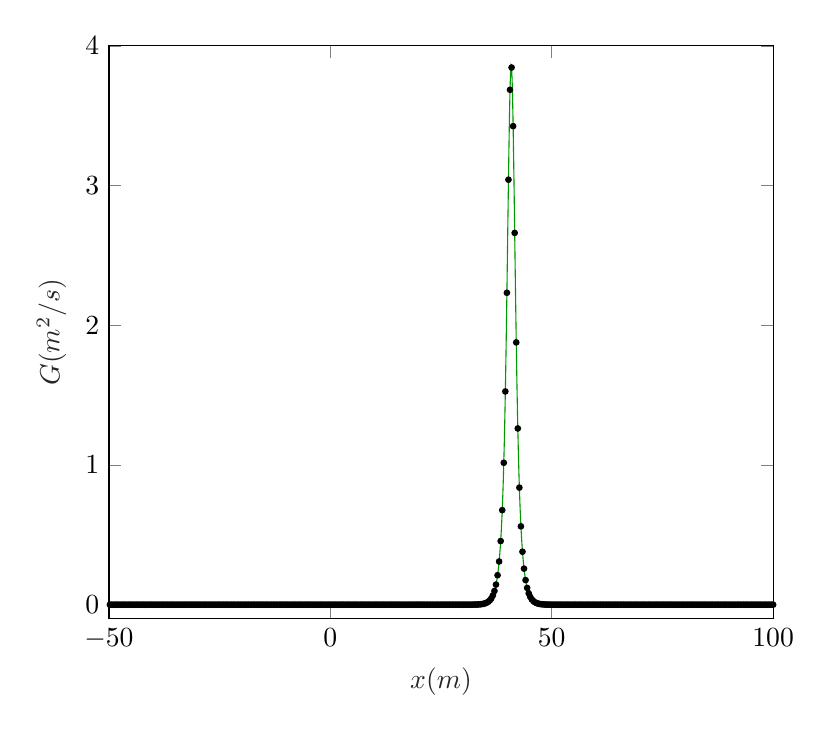
\begin{tikzpicture}

\begin{axis}[%
scale only axis,
xmin=-50,
xmax=100,
xtick={-50,   0,  50, 100},
xlabel style={font=\color{white!15!black}},
xlabel={$x (m)$},
ymin=-0.1,
ymax=4,
ytick={0, 1, 2, 3, 4},
ylabel style={font=\color{white!15!black}},
ylabel={$G (m^2/s)$},
axis background/.style={fill=white}
]
\addplot [color=green!60!black, forget plot]
  table[row sep=crcr]{%
-50.14064697609	-5.67925565028477e-44\\
-50.0234411626817	-6.46942449732437e-44\\
-49.9062353492733	-7.36953148507789e-44\\
-49.789029535865	-8.39487257823589e-44\\
-49.6718237224566	-9.56287190678446e-44\\
-49.5546179090483	-1.08933778628938e-43\\
-49.4374120956399	-1.2409000394494e-43\\
-49.3202062822316	-1.41354952273408e-43\\
-49.2030004688233	-1.61022015448423e-43\\
-49.0857946554149	-1.83425405633628e-43\\
-48.9685888420066	-2.08945834755365e-43\\
-48.8513830285982	-2.38016984129328e-43\\
-48.7341772151899	-2.71132874222405e-43\\
-48.6169714017815	-3.08856259787573e-43\\
-48.4997655883732	-3.51828193034678e-43\\
-48.3825597749648	-4.00778917348764e-43\\
-48.2653539615565	-4.56540276678192e-43\\
-48.1481481481481	-5.20059851471748e-43\\
-48.0309423347398	-5.92417061383291e-43\\
-47.9137365213315	-6.74841508385664e-43\\
-47.7965307079231	-7.68733872007089e-43\\
-47.6793248945148	-8.75689711773463e-43\\
-47.5621190811064	-9.97526581343133e-43\\
-47.4449132676981	-1.13631491509804e-42\\
-47.3277074542897	-1.29441321206272e-42\\
-47.2105016408814	-1.47450811504829e-42\\
-47.093295827473	-1.6796600661072e-42\\
-46.9760900140647	-1.91335531414344e-42\\
-46.8588842006564	-2.17956515847011e-42\\
-46.741678387248	-2.4828134350695e-42\\
-46.6244725738397	-2.82825339238234e-42\\
-46.5072667604313	-3.22175526301613e-42\\
-46.390060947023	-3.67000601952039e-42\\
-46.2728551336146	-4.18062300942952e-42\\
-46.1556493202063	-4.76228340062936e-42\\
-46.0384435067979	-5.42487163677648e-42\\
-45.9212376933896	-6.17964740855479e-42\\
-45.8040318799812	-7.03943699518549e-42\\
-45.6868260665729	-8.0188512277557e-42\\
-45.5696202531646	-9.13453377832024e-42\\
-45.4524144397562	-1.04054439940802e-41\\
-45.3352086263479	-1.18531790829781e-41\\
-45.2180028129395	-1.3502341125768e-41\\
-45.1007969995312	-1.53809551513841e-41\\
-44.9835911861228	-1.7520945380161e-41\\
-44.8663853727145	-1.99586777279541e-41\\
-44.7491795593061	-2.27355777901906e-41\\
-44.6319737458978	-2.58988348075698e-41\\
-44.5147679324894	-2.95022035762469e-41\\
-44.3975621190811	-3.36069179297554e-41\\
-44.2803563056728	-3.82827313159305e-41\\
-44.1631504922644	-4.36091021518543e-41\\
-44.0459446788561	-4.96765441001729e-41\\
-43.9287388654477	-5.65881642126743e-41\\
-43.8115330520394	-6.44614150795858e-41\\
-43.694327238631	-7.34300907597218e-41\\
-43.5771214252227	-8.36466004093106e-41\\
-43.4599156118143	-9.52845582464262e-41\\
-43.342709798406	-1.08541733863529e-40\\
-43.2255039849977	-1.23643413024305e-40\\
-43.1082981715893	-1.40846226056424e-40\\
-42.991092358181	-1.60442508898053e-40\\
-42.8738865447726	-1.827652709075e-40\\
-42.7566807313643	-2.081938538565e-40\\
-42.6394749179559	-2.3716037827318e-40\\
-42.5222691045476	-2.70157086680588e-40\\
-42.4050632911392	-3.07744708518192e-40\\
-42.2878574777309	-3.50561988895448e-40\\
-42.1706516643225	-3.99336543104426e-40\\
-42.0534458509142	-4.54897221347495e-40\\
-41.9362400375059	-5.18188193800127e-40\\
-41.8190342240975	-5.90284995363215e-40\\
-41.7018284106892	-6.72412802761265e-40\\
-41.5846225972808	-7.65967254578537e-40\\
-41.4674167838725	-8.72538168037957e-40\\
-41.3502109704641	-9.93936555554129e-40\\
-41.2330051570558	-1.13222540016589e-39\\
-41.1157993436474	-1.28975471283085e-39\\
-40.9985935302391	-1.46920146732771e-39\\
-40.8813877168308	-1.67361509139989e-39\\
-40.7641819034224	-1.90646928719458e-39\\
-40.6469760900141	-2.17172106160686e-39\\
-40.5297702766057	-2.47387796966146e-39\\
-40.4125644631974	-2.81807471363196e-39\\
-40.295358649789	-3.21016039958451e-39\\
-40.1781528363807	-3.65679793413976e-39\\
-40.0609470229723	-4.16557725055085e-39\\
-39.943741209564	-4.74514428820606e-39\\
-39.8265353961556	-5.40534791736657e-39\\
-39.7093295827473	-6.1574073059063e-39\\
-39.592123769339	-7.01410257219832e-39\\
-39.4749179559306	-7.98999196400849e-39\\
-39.3577121425223	-9.10165925402394e-39\\
-39.2405063291139	-1.03679955561304e-38\\
-39.1233005157056	-1.1810520351486e-38\\
-39.0060947022972	-1.3453747179742e-38\\
-38.8888888888889	-1.53256002097858e-38\\
-38.7716830754805	-1.74578887690003e-38\\
-38.6544772620722	-1.98868478949472e-38\\
-38.5372714486639	-2.26537540953428e-38\\
-38.4200656352555	-2.58056267802317e-38\\
-38.3028598218472	-2.93960272861585e-38\\
-38.1856540084388	-3.34859690705341e-38\\
-38.0684481950305	-3.81449545435936e-38\\
-37.9512423816221	-4.34521561573435e-38\\
-37.8340365682138	-4.94977618223231e-38\\
-37.7168307548054	-5.63845075155249e-38\\
-37.5996249413971	-6.42294231238227e-38\\
-37.4824191279887	-7.31658211909224e-38\\
-37.3652133145804	-8.3345562363561e-38\\
-37.2480075011721	-9.49416360348316e-38\\
-37.1308016877637	-1.08151100038787e-37\\
-37.0135958743554	-1.2319842935199e-37\\
-36.896390060947	-1.40339330708186e-37\\
-36.7791842475387	-1.59865087949707e-37\\
-36.6619784341303	-1.82107511958348e-37\\
-36.544772620722	-2.07444579282335e-37\\
-36.4275668073136	-2.36306855279352e-37\\
-36.3103609939053	-2.69184810927339e-37\\
-36.193155180497	-3.06637157641179e-37\\
-36.0759493670886	-3.49300341733039e-37\\
-35.9587435536803	-3.97899359860334e-37\\
-35.8415377402719	-4.53260079253712e-37\\
-35.7243319268636	-5.16323272088679e-37\\
-35.6071261134552	-5.88160602494042e-37\\
-35.4899203000469	-6.699928378722e-37\\
-35.3727144866385	-7.63210594005375e-37\\
-35.2555086732302	-8.69397966479689e-37\\
-35.1383028598218	-9.90359450007444e-37\\
-35.0210970464135	-1.12815060310125e-36\\
-34.9038912330052	-1.28511297919975e-36\\
-34.7866854195968	-1.46391391784721e-36\\
-34.6694796061885	-1.66759187211797e-36\\
-34.5522737927801	-1.89960804255711e-36\\
-34.4350679793718	-2.16390519507907e-36\\
-34.3178621659634	-2.46497466234507e-36\\
-34.2006563525551	-2.80793266720784e-36\\
-34.0834505391467	-3.19860726522513e-36\\
-33.9662447257384	-3.64363738370003e-36\\
-33.8490389123301	-4.15058564026676e-36\\
-33.7318330989217	-4.72806685820487e-36\\
-33.6146272855134	-5.38589446240624e-36\\
-33.497421472105	-6.13524724377348e-36\\
-33.3802156586967	-6.98885932596121e-36\\
-33.2630098452883	-7.96123656265768e-36\\
-33.14580403188	-9.06890304275518e-36\\
-33.0285982184716	-1.03306818923917e-35\\
-32.9113924050633	-1.17680151456735e-35\\
-32.7941865916549	-1.34053281198016e-35\\
-32.6769807782466	-1.52704444866057e-35\\
-32.5597749648383	-1.73950590940077e-35\\
-32.4425691514299	-1.98152765722979e-35\\
-32.3253633380216	-2.25722248780352e-35\\
-32.2081575246132	-2.57127542018214e-35\\
-32.0909517112049	-2.92902331168347e-35\\
-31.9737458977965	-3.33654554974806e-35\\
-31.8565400843882	-3.80076736198637e-35\\
-31.7393342709798	-4.32957750000788e-35\\
-31.6221284575715	-4.93196229689201e-35\\
-31.5049226441632	-5.61815837640502e-35\\
-31.3877168307548	-6.39982660902768e-35\\
-31.2705110173465	-7.29025027091278e-35\\
-31.1533052039381	-8.30456077318933e-35\\
-31.0360993905298	-9.45999479753952e-35\\
-30.9188935771214	-1.07761872076836e-34\\
-30.8016877637131	-1.22755047143627e-34\\
-30.6844819503047	-1.39834259639528e-34\\
-30.5672761368964	-1.59289745097464e-34\\
-30.450070323488	-1.81452120235933e-34\\
-30.3328645100797	-2.06698001292991e-34\\
-30.2156586966714	-2.3545640405285e-34\\
-30.098452883263	-2.68216034323976e-34\\
-29.9812470698547	-3.05533592759417e-34\\
-29.8640412564463	-3.48043235147226e-34\\
-29.746835443038	-3.96467348934472e-34\\
-29.6296296296296	-4.51628829115533e-34\\
-29.5124238162213	-5.14465062095144e-34\\
-29.3952180028129	-5.86043855160665e-34\\
-29.2780121894046	-6.67581582261175e-34\\
-29.1608063759962	-7.60463854453612e-34\\
-29.0436005625879	-8.66269066278986e-34\\
-28.9263947491796	-9.86795218204107e-34\\
-28.8091889357712	-1.12409047093557e-33\\
-28.6919831223629	-1.28048795083117e-33\\
-28.5747773089545	-1.45864539787368e-33\\
-28.4575714955462	-1.6615903299652e-33\\
-28.3403656821378	-1.89277149104129e-33\\
-28.2231598687295	-2.15611745728783e-33\\
-28.1059540553211	-2.45610339738575e-33\\
-27.9887482419128	-2.79782712127288e-33\\
-27.8715424285045	-3.18709570975801e-33\\
-27.7543366150961	-3.63052419712644e-33\\
-27.6371308016878	-4.13564798370029e-33\\
-27.5199249882794	-4.71105088863525e-33\\
-27.4027191748711	-5.36651101901884e-33\\
-27.2855133614627	-6.11316693409651e-33\\
-27.1683075480544	-6.96370692833562e-33\\
-27.051101734646	-7.93258464990982e-33\\
-26.9338959212377	-9.03626471871409e-33\\
-26.8166901078293	-1.02935025178213e-32\\
-26.699484294421	-1.17256629130129e-32\\
-26.5822784810127	-1.33570833165449e-32\\
-26.4650726676043	-1.52154872648717e-32\\
-26.347866854196	-1.73324555384564e-32\\
-26.2306610407876	-1.97439628296455e-32\\
-26.1134552273793	-2.24909890784659e-32\\
-25.9962494139709	-2.5620215865082e-32\\
-25.8790436005626	-2.91848196930506e-32\\
-25.7618377871542	-3.32453756440329e-32\\
-25.6446319737459	-3.78708867602171e-32\\
-25.5274261603376	-4.3139956647252e-32\\
-25.4102203469292	-4.91421252243247e-32\\
-25.2930145335209	-5.59793903204352e-32\\
-25.1758087201125	-6.37679409741217e-32\\
-25.0586029067042	-7.26401318914445e-32\\
-24.9413970932958	-8.27467326151825e-32\\
-24.8241912798875	-9.42594896264916e-32\\
-24.7069854664791	-1.07374044918077e-31\\
-24.5897796530708	-1.22313260635659e-31\\
-24.4725738396624	-1.39331006285001e-31\\
-24.3553680262541	-1.58716472862398e-31\\
-24.2381622128458	-1.80799087220775e-31\\
-24.1209563994374	-2.05954110183665e-31\\
-24.0037505860291	-2.34609013538603e-31\\
-23.8865447726207	-2.67250744277318e-31\\
-23.7693389592124	-3.04433999527589e-31\\
-23.652133145804	-3.46790652796809e-31\\
-23.5349273323957	-3.95040491712024e-31\\
-23.4177215189873	-4.50003449728256e-31\\
-23.300515705579	-5.12613539664557e-31\\
-23.1833098921707	-5.83934725847349e-31\\
-23.0661040787623	-6.65179004584142e-31\\
-22.948898265354	-7.5772700021819e-31\\
-22.8316924519456	-8.63151426763096e-31\\
-22.7144866385373	-9.83243813812407e-31\\
-22.5972808251289	-1.120044950891e-30\\
-22.4800750117206	-1.27587956760414e-30\\
-22.3628691983122	-1.45339583892122e-30\\
-22.2456633849039	-1.65561038692719e-30\\
-22.1284575714955	-1.88595954377831e-30\\
-22.0112517580872	-2.14835774699988e-30\\
-21.8940459446789	-2.44726405946538e-30\\
-21.7768401312705	-2.7877579444646e-30\\
-21.6596343178622	-3.17562558354374e-30\\
-21.5424285044538	-3.61745820395983e-30\\
-21.4252226910455	-4.12076408667597e-30\\
-21.3080168776371	-4.69409615830541e-30\\
-21.1908110642288	-5.34719733523786e-30\\
-21.0736052508204	-6.09116608985208e-30\\
-20.9563994374121	-6.93864505236433e-30\\
-20.8391936240038	-7.90403585331695e-30\\
-20.7219878105954	-9.0037438576331e-30\\
-20.6047819971871	-1.02564569491223e-29\\
-20.4875761837787	-1.16834631029645e-29\\
-20.3703703703704	-1.33090121428349e-29\\
-20.253164556962	-1.51607278301914e-29\\
-20.1359587435537	-1.72700772885597e-29\\
-20.0187529301453	-1.96729057399784e-29\\
-19.901547116737	-2.24100456406447e-29\\
-19.7843413033286	-2.55280105671022e-29\\
-19.6671354899203	-2.90797856445299e-29\\
-19.549929676512	-3.31257279492657e-29\\
-19.4327238631036	-3.77345921865547e-29\\
-19.3155180496953	-4.29846990733726e-29\\
-19.1983122362869	-4.89652662812327e-29\\
-19.0811064228786	-5.57779245563524e-29\\
-18.9639006094702	-6.35384447813479e-29\\
-18.8466947960619	-7.23787053272964e-29\\
-18.7294889826535	-8.24489331283325e-29\\
-18.6122831692452	-9.39202565624859e-29\\
-18.4950773558368	-1.06987613521126e-28\\
-18.3778715424285	-1.21873064085278e-28\\
-18.2606657290202	-1.38829564102781e-28\\
-18.1434599156118	-1.58145263792512e-28\\
-18.0262541022035	-1.80148404424055e-28\\
-17.9090482887951	-2.0521289628447e-28\\
-17.7918424753868	-2.3376467272134e-28\\
-17.6746366619784	-2.66288928239499e-28\\
-17.5574308485701	-3.03338363652019e-28\\
-17.4402250351617	-3.45542578399383e-28\\
-17.3230192217534	-3.93618769645192e-28\\
-17.2058134083451	-4.48383919963454e-28\\
-17.0886075949367	-5.10768680728865e-28\\
-16.9714017815284	-5.81833187137416e-28\\
-16.85419596812	-6.62785073609845e-28\\
-16.7369901547117	-7.54999995722585e-28\\
-16.6197843413033	-8.60045007405599e-28\\
-16.502578527895	-9.79705190667434e-28\\
-16.3853727144866	-1.11601399037952e-27\\
-16.2681669010783	-1.27128776961395e-27\\
-16.1509610876699	-1.44816517275059e-27\\
-16.0337552742616	-1.64965196527029e-27\\
-15.9165494608533	-1.87917211221926e-27\\
-15.7993436474449	-2.14062596334618e-27\\
-15.6821378340366	-2.4384565336808e-27\\
-15.5649320206282	-2.77772500589302e-27\\
-15.4477262072199	-3.16419673748154e-27\\
-15.3305203938115	-3.6044392343547e-27\\
-15.2133145804032	-4.10593375571712e-27\\
-15.0961087669948	-4.67720244681982e-27\\
-14.9789029535865	-5.32795316000339e-27\\
-14.8616971401782	-6.06924442504969e-27\\
-14.7444913267698	-6.91367337226614e-27\\
-14.6272855133615	-7.87558980177177e-27\\
-14.5100796999531	-8.97134003677153e-27\\
-14.3928738865448	-1.02195447047372e-26\\
-14.2756680731364	-1.16414151669705e-26\\
-14.1584622597281	-1.3261113973791e-26\\
-14.0412564463197	-1.51061654707431e-26\\
-13.9240506329114	-1.72079235334581e-26\\
-13.806844819503	-1.96021043796217e-26\\
-13.6896390060947	-2.23293935123833e-26\\
-13.5724331926864	-2.54361371092997e-26\\
-13.455227379278	-2.89751296059287e-26\\
-13.3380215658697	-3.30065108578702e-26\\
-13.2208157524613	-3.75987881271732e-26\\
-13.103609939053	-4.28300002602356e-26\\
-12.9864041256446	-4.87890438406459e-26\\
-12.8691983122363	-5.55771838529369e-26\\
-12.7519924988279	-6.33097745287205e-26\\
-12.6347866854196	-7.21182196183838e-26\\
-12.5175808720113	-8.21522054002271e-26\\
-12.4003750586029	-9.35822443736625e-26\\
-12.2831692451946	-1.06602572862732e-25\\
-12.1659634317862	-1.21434451770346e-25\\
-12.0487576183779	-1.38329926574592e-25\\
-11.9315518049695	-1.57576110462623e-25\\
-11.8143459915612	-1.79500063387508e-25\\
-11.6971401781528	-2.04474349960316e-25\\
-11.5799343647445	-2.32923370625412e-25\\
-11.4627285513361	-2.65330573707812e-25\\
-11.3455227379278	-3.0224667089047e-25\\
-11.2283169245195	-3.44298995731157e-25\\
-11.1111111111111	-3.9220216425292e-25\\
-10.9939052977028	-4.46770218768769e-25\\
-10.8766994842944	-5.08930461306618e-25\\
-10.7594936708861	-5.79739211712812e-25\\
-10.6422878574777	-6.60399758219424e-25\\
-10.5250820440694	-7.52282805518297e-25\\
-10.407876230661	-8.56949767825991e-25\\
-10.2906704172527	-9.76179302770403e-25\\
-10.1734646038444	-1.11199753700245e-24\\
-10.056258790436	-1.26671249717158e-24\\
-9.93905297702766	-1.44295333136797e-24\\
-9.82184716361932	-1.64371498754059e-24\\
-9.70464135021097	-1.87240910813395e-24\\
-9.58743553680262	-2.1329220058209e-24\\
-9.47022972339428	-2.42968070554245e-24\\
-9.35302390998594	-2.7677281751394e-24\\
-9.23581809657759	-3.15280902300708e-24\\
-9.11861228316924	-3.59146711907652e-24\\
-9.0014064697609	-4.09115679804335e-24\\
-8.88420065635255	-4.66036953457618e-24\\
-8.76699484294421	-5.30877824315931e-24\\
-8.64978902953587	-6.04740165472831e-24\\
-8.53258321612752	-6.88879156343276e-24\\
-8.41537740271917	-7.84724612550216e-24\\
-8.29817158931083	-8.93905283491006e-24\\
-8.18096577590249	-1.01827653048414e-23\\
-8.06375996249414	-1.15995185584475e-23\\
-7.94655414908579	-1.32133881867822e-23\\
-7.82934833567745	-1.50517994772675e-23\\
-7.7121425222691	-1.71459934652117e-23\\
-7.59493670886076	-1.95315578282238e-23\\
-7.47773089545242	-2.22490316452794e-23\\
-7.36052508204407	-2.53445942974058e-23\\
-7.24331926863572	-2.88708502168173e-23\\
-7.12611345522738	-3.28877228201366e-23\\
-7.00890764181904	-3.7463472816748e-23\\
-6.89170182841069	-4.26758581969034e-23\\
-6.77449601500234	-4.8613455611836e-23\\
-6.657290201594	-5.53771656007476e-23\\
-6.54008438818565	-6.30819272437408e-23\\
-6.42287857477731	-7.18586713786387e-23\\
-6.30567276136896	-8.18565455736856e-23\\
-6.18846694796062	-9.32454486661817e-23\\
-6.07126113455227	-1.06218917937732e-22\\
-5.95405532114393	-1.20997417989309e-22\\
-5.83684950773559	-1.37832087205614e-22\\
-5.71964369432724	-1.57009005474272e-22\\
-5.60243788091889	-1.78854055683312e-22\\
-5.48523206751055	-2.03738461610793e-22\\
-5.3680262541022	-2.32085096314685e-22\\
-5.25082044069386	-2.64375668224554e-22\\
-5.13361462728551	-3.0115890705196e-22\\
-5.01640881387717	-3.43059888626723e-22\\
-4.89920300046882	-3.90790657120676e-22\\
-4.78199718706048	-4.45162325167598e-22\\
-4.66479137365214	-5.07098857502693e-22\\
-4.54758556024379	-5.77652772353829e-22\\
-4.43037974683544	-6.58023027406032e-22\\
-4.31317393342709	-7.49575394284404e-22\\
-4.19596812001875	-8.53865667789042e-22\\
-4.07876230661041	-9.726661042881e-22\\
-3.96155649320206	-1.10799553854966e-21\\
-3.84435067979372	-1.26215369080274e-21\\
-3.72714486638537	-1.43776024702432e-21\\
-3.60993905297703	-1.637799376563e-21\\
-3.49273323956868	-1.86567044360962e-21\\
-3.37552742616034	-2.12524577427976e-21\\
-3.25832161275199	-2.42093646097287e-21\\
-3.14111579934364	-2.75776732225433e-21\\
-3.0239099859353	-3.14146229209073e-21\\
-2.90670417252696	-3.57854168950001e-21\\
-2.78949835911861	-4.07643302156808e-21\\
-2.67229254571027	-4.6435972027623e-21\\
-2.55508673230192	-5.28967233544967e-21\\
-2.43788091889358	-6.02563749495257e-21\\
-2.32067510548523	-6.86399930242403e-21\\
-2.20346929207689	-7.81900445606685e-21\\
-2.08626347866854	-8.90688183234557e-21\\
-1.96905766526019	-1.01461182713373e-20\\
-1.85185185185185	-1.15577727327786e-20\\
-1.73464603844351	-1.3165834161418e-20\\
-1.61744022503516	-1.4997629143058e-20\\
-1.50023441162681	-1.70842862787873e-20\\
-1.38302859821847	-1.94612651687457e-20\\
-1.26582278481013	-2.21689589947048e-20\\
-1.14861697140178	-2.52533809414499e-20\\
-1.03141115799344	-2.87669461216609e-20\\
-0.914205344585092	-3.2769362291932e-20\\
-0.796999531176745	-3.73286444963069e-20\\
-0.679793717768398	-4.2522270879673e-20\\
-0.562587904360058	-4.84384993123216e-20\\
-0.445382090951711	-5.51778671997359e-20\\
-0.328176277543363	-6.28548999646078e-20\\
-0.210970464135023	-7.16000572341759e-20\\
-0.0937646507266763	-8.15619498054077e-20\\
0.0234411626816708	-9.29098650620153e-20\\
0.140646976090011	-1.05836643758969e-19\\
0.257852789498358	-1.2056195706114e-19\\
0.375058602906705	-1.37336039524405e-19\\
0.492264416315052	-1.56443941455628e-19\\
0.609470229723392	-1.7821037291397e-19\\
0.726676043131739	-2.03005221670051e-19\\
0.843881856540087	-2.3124983889238e-19\\
0.961087669948427	-2.63424199376843e-19\\
1.07829348335677	-3.0007505799658e-19\\
1.19549929676512	-3.41825240978853e-19\\
1.31270511017347	-3.89384229900186e-19\\
1.42991092358181	-4.43560218258835e-19\\
1.54711673699016	-5.0527384550797e-19\\
1.6643225503985	-5.75573841938713e-19\\
1.78152836380684	-6.55654850274386e-19\\
1.89873417721519	-7.468777268271e-19\\
2.01593999062354	-8.50792667204355e-19\\
2.13314580403188	-9.69165549552229e-19\\
2.25035161744022	-1.10400794299894e-18\\
2.36755743084857	-1.25761129124728e-18\\
2.48476324425692	-1.43258585221445e-18\\
2.60196905766526	-1.63190505544009e-18\\
2.71917487107361	-1.85895603104999e-18\\
2.83638068448195	-2.11759716893897e-18\\
2.95358649789029	-2.41222368630501e-18\\
3.07079231129864	-2.74784231775607e-18\\
3.18799812470699	-3.13015639723567e-18\\
3.30520393811533	-3.56566277760675e-18\\
3.42240975152367	-4.06176223489603e-18\\
3.53961556493202	-4.62688523335374e-18\\
3.65682137834037	-5.27063518851562e-18\\
3.77402719174871	-6.00395166280868e-18\\
3.89123300515705	-6.83929626696383e-18\\
4.0084388185654	-7.79086442635072e-18\\
4.12564463197375	-8.87482661088508e-18\\
4.24285044538209	-1.01096031278477e-17\\
4.36005625879044	-1.15161771473073e-17\\
4.47726207219878	-1.31184512795408e-17\\
4.59446788560712	-1.49436537639508e-17\\
4.71167369901547	-1.70228011720496e-17\\
4.82887951242382	-1.93912254874488e-17\\
4.94608532583216	-2.20891745197898e-17\\
5.0632911392405	-2.51624958557439e-17\\
5.18049695264885	-2.86634159698041e-17\\
5.2977027660572	-3.26514277346808e-17\\
5.41490857946554	-3.71943014132084e-17\\
5.53211439287389	-4.23692363120529e-17\\
5.64932020628223	-4.82641726678348e-17\\
5.76652601969058	-5.49792860592091e-17\\
5.88373183309892	-6.262868974018e-17\\
6.00093764650727	-7.13423738232549e-17\\
6.11814345991561	-8.12684142659256e-17\\
6.23534927332395	-9.25754891988914e-17\\
6.3525550867323	-1.0545574535724e-16\\
6.46976090014065	-1.20128063325257e-16\\
6.58696671354899	-1.36841777082808e-16\\
6.70417252695734	-1.55880911061387e-16\\
6.82137834036568	-1.77569006712211e-16\\
6.93858415377403	7.04499652447659e-16\\
7.05578996718237	6.76356685553378e-16\\
7.17299578059072	6.44298118257833e-16\\
7.29020159399906	6.07779163419e-16\\
7.4074074074074	5.66179236316026e-16\\
7.52461322081575	5.187914087451e-16\\
7.6418190342241	4.6481039583772e-16\\
7.75902484763245	4.03318871455313e-16\\
7.87623066104079	1.2400461526653e-15\\
7.99343647444913	1.16025335006822e-15\\
8.11064228785748	1.06935877802938e-15\\
8.22784810126582	9.6581781998282e-16\\
8.34505391467417	1.75464522610409e-15\\
8.46225972808251	1.62028812064766e-15\\
8.57946554149086	1.46723757970471e-15\\
8.6966713548992	2.19966701254122e-15\\
8.81387716830755	2.00106514466603e-15\\
8.9310829817159	2.68160558209758e-15\\
9.04828879512424	3.33066954795203e-15\\
9.16549460853258	3.03710337004486e-15\\
9.28270042194093	3.60946687875131e-15\\
9.39990623534927	4.13530299295864e-15\\
9.51711204875762	5.51491251456027e-15\\
9.63431786216596	5.92737275627671e-15\\
9.75152367557431	6.27105786754127e-15\\
9.86872948898265	7.4431732678683e-15\\
9.985935302391	8.52604449246784e-15\\
10.1031411157993	9.50725477904178e-15\\
10.2203469292077	1.12794340635809e-14\\
10.337552742616	1.2919695799463e-14\\
10.4547585560244	1.44096859727564e-14\\
10.5719643694327	1.66352712033538e-14\\
10.6891701828411	1.8665860631684e-14\\
10.8063759962494	2.13810982838562e-14\\
10.9235818096578	2.38433049416946e-14\\
11.0407876230661	2.78308243249419e-14\\
11.1579934364744	3.14900049267945e-14\\
11.2751992498828	3.56819384357729e-14\\
11.3924050632911	4.03545863366771e-14\\
11.5096108766995	4.63554441403836e-14\\
11.6268166901078	5.27102112112611e-14\\
11.7440225035162	6.02487403504022e-14\\
11.8612283169245	6.88834078117178e-14\\
11.9784341303329	7.85143985411919e-14\\
12.0956399437412	8.90280099701405e-14\\
12.2128457571496	1.01201494084096e-13\\
12.3300515705579	1.15794082113248e-13\\
12.4472573839662	1.31730928714194e-13\\
12.5644631973746	1.49727352947061e-13\\
12.6816690107829	1.71378810509016e-13\\
12.7988748241913	1.94623316208983e-13\\
12.9160806375996	2.21898190617956e-13\\
13.033286451008	2.52881056686928e-13\\
13.1504922644163	2.88111458525937e-13\\
13.2676980778247	3.28077846606643e-13\\
13.384903891233	3.73210468978376e-13\\
13.5021097046413	4.2568682196768e-13\\
13.6193155180497	4.84888554293072e-13\\
13.736521331458	5.51924830480177e-13\\
13.8537271448664	6.28713586641477e-13\\
13.9709329582747	7.17061120847776e-13\\
14.0881387716831	8.15926237832966e-13\\
14.2053445850914	9.29563523903678e-13\\
14.3225503984998	1.05934222318704e-12\\
14.4397562119081	1.20644360089922e-12\\
14.5569620253165	1.37455511219495e-12\\
14.6741678387248	1.56621351223959e-12\\
14.7913736521331	1.78367769249551e-12\\
14.9085794655415	2.0316103436789e-12\\
15.0257852789498	2.31431359423626e-12\\
15.1429910923582	2.63658561869945e-12\\
15.2601969057665	3.00366349205996e-12\\
15.3774027191749	3.42115809333096e-12\\
15.4946085325832	3.89770027490109e-12\\
15.6118143459916	4.43941574627565e-12\\
15.7290201593999	5.05708304503515e-12\\
15.8462259728083	5.76058328019619e-12\\
15.9634317862166	6.56240236785392e-12\\
16.0806375996249	7.47567524890499e-12\\
16.1978434130333	8.51583741453226e-12\\
16.3150492264416	9.70044034047623e-12\\
16.43225503985	1.10498480164934e-11\\
16.5494608532583	1.25869974496629e-11\\
16.6666666666667	1.43389393944725e-11\\
16.783872480075	1.63338072536351e-11\\
16.9010782934834	1.86059037082805e-11\\
17.0182841068917	2.11943906731916e-11\\
17.1354899203	2.41437366925726e-11\\
17.2526957337084	2.75022868728026e-11\\
17.3699015471167	3.13289209766071e-11\\
17.4871073605251	3.56878405148137e-11\\
17.6043131739334	4.06532358790363e-11\\
17.7215189873418	4.63093119822287e-11\\
17.8387248007501	5.27529116277478e-11\\
17.9559306141585	6.00923721301736e-11\\
18.0731364275668	6.84534770491427e-11\\
18.1903422409752	7.79779725144793e-11\\
18.3075480543835	8.88264109953478e-11\\
18.4247538677918	1.01185293792682e-10\\
18.5419596812002	1.15263971149788e-10\\
18.6591654946085	1.31300304972158e-10\\
18.7763713080169	1.49568704282621e-10\\
18.8935771214252	1.70378696985551e-10\\
19.0107829348336	1.94083931884914e-10\\
19.1279887482419	2.21087039813816e-10\\
19.2451945616503	2.51847536584693e-10\\
19.3624003750586	2.86887245683508e-10\\
19.4796061884669	3.26803122464384e-10\\
19.5968120018753	3.72271959015278e-10\\
19.7140178152836	4.2406679836046e-10\\
19.831223628692	4.8306859894736e-10\\
19.9484294421003	5.50279340645031e-10\\
20.0656352555087	6.2684092820148e-10\\
20.182841068917	7.14054248834957e-10\\
20.3000468823254	8.134026869523e-10\\
20.4172526957337	9.26573485573149e-10\\
20.5344585091421	1.05548934970686e-09\\
20.6516643225504	1.20234269621174e-09\\
20.7688701359587	1.36962762750629e-09\\
20.8860759493671	1.56018732177038e-09\\
21.0032817627754	1.77726001323682e-09\\
21.1204875761838	2.02453477599012e-09\\
21.2376933895921	2.30621282957294e-09\\
21.3548992030005	2.62708178169132e-09\\
21.4721050164088	2.99259470439821e-09\\
21.5893108298172	3.40896123711507e-09\\
21.7065166432255	3.88325868200008e-09\\
21.8237224566338	4.42354642090899e-09\\
21.9409282700422	5.039004893022e-09\\
22.0581340834505	5.74009387675532e-09\\
22.1753398968589	6.53872731321492e-09\\
22.2925457102672	7.44847706538602e-09\\
22.4097515236756	8.48480229793672e-09\\
22.5269573370839	9.66531352227517e-09\\
22.6441631504923	1.10100718088318e-08\\
22.7613689639006	1.25419304879271e-08\\
22.878574777309	1.42869207246381e-08\\
22.9957805907173	1.62746953904763e-08\\
23.1129864041256	1.85390327705267e-08\\
23.230192217534	2.11184149675598e-08\\
23.3473980309423	2.40566719078874e-08\\
23.4646038443507	2.74037357635419e-08\\
23.581809657759	3.12164851421731e-08\\
23.6990154711674	3.55597115697239e-08\\
23.8162212845757	4.05072217045498e-08\\
23.9334270979841	4.61430921092188e-08\\
24.0506329113924	5.25630938509119e-08\\
24.1678387248007	5.98763261550833e-08\\
24.2850445382091	6.82070678624435e-08\\
24.4022503516174	7.76968853896477e-08\\
24.5194561650258	8.85070437070075e-08\\
24.6366619784341	1.00821247029413e-07\\
24.7538677918425	1.1484875460448e-07\\
24.8710736052508	1.30827945090361e-07\\
24.9882794186592	1.49030359311305e-07\\
25.1054852320675	1.69765320102649e-07\\
25.2226910454759	1.93385186342083e-07\\
25.3398968588842	2.20291342766761e-07\\
25.4571026722925	2.50941018476639e-07\\
25.5743084857009	2.85855058826503e-07\\
25.6915142991092	3.25626774548931e-07\\
25.8087201125176	3.70932027150908e-07\\
25.9259259259259	4.22540709487775e-07\\
26.0431317393343	4.81329833101205e-07\\
26.1603375527426	5.4829843077014e-07\\
26.277543366151	6.24584532254987e-07\\
26.3947491795593	7.1148450277315e-07\\
26.5119549929676	8.10475075926028e-07\\
26.629160806376	9.23238446084501e-07\\
26.7463666197843	1.05169085352027e-06\\
26.8635724331927	1.19801515152588e-06\\
26.980778246601	1.3646978958533e-06\\
27.0979840600094	1.55457160478368e-06\\
27.2151898734177	1.77086288830396e-06\\
27.3323956868261	2.01724728352007e-06\\
27.4496015002344	2.29791170841468e-06\\
27.5668073136428	2.61762561877808e-06\\
27.6840131270511	2.98182205022739e-06\\
27.8012189404594	3.39668994642382e-06\\
27.9184247538678	3.86927932937337e-06\\
28.0356305672761	4.40762109996003e-06\\
28.1528363806845	5.02086350780401e-06\\
28.2700421940928	5.71942760981789e-06\\
28.3872480075012	6.51518435488633e-06\\
28.5044538209095	7.42165630450217e-06\\
28.6216596343179	8.454247420254e-06\\
28.7388654477262	9.63050481972133e-06\\
28.8560712611346	1.09704169509731e-05\\
28.9732770745429	1.24967532438382e-05\\
29.0904828879512	1.42354510177999e-05\\
29.2076887013596	1.62160562181099e-05\\
29.3248945147679	1.84722254612266e-05\\
29.4421003281763	2.10422979253289e-05\\
29.5593061415846	2.39699467943057e-05\\
29.676511954993	2.73049213320218e-05\\
29.7937177684013	3.11038921735575e-05\\
29.9109235818097	3.543141420647e-05\\
30.028129395218	4.03610233869567e-05\\
30.1453352086263	4.59764861124935e-05\\
30.2625410220347	5.23732223738739e-05\\
30.379746835443	5.96599268373539e-05\\
30.4969526488514	6.79604153903211e-05\\
30.6141584622597	7.74157284720337e-05\\
30.7313642756681	8.81865268958671e-05\\
30.8485700890764	0.000100455820813016\\
30.9657759024848	0.000114432078097946\\
31.0829817158931	0.000130352764879346\\
31.2001875293015	0.000148488378236566\\
31.3173933427098	0.000169147039410214\\
31.4345991561181	0.000192679725343126\\
31.5518049695265	0.000219486227146894\\
31.6690107829348	0.000250021936355717\\
31.7862165963432	0.000284805573764508\\
31.9034224097515	0.000324427991524394\\
32.0206282231599	0.00036956219721324\\
32.1378340365682	0.00042097476908627\\
32.2550398499766	0.000479538855050475\\
32.3722456633849	0.000546248974354167\\
32.4894514767932	0.000622237871096495\\
32.6066572902016	0.000708795702770705\\
32.7238631036099	0.000807391885842149\\
32.8410689170183	0.000919699964270065\\
32.9582747304266	0.00104762591672266\\
33.075480543835	0.00119334037464924\\
33.1926863572433	0.00135931528724505\\
33.3098921706517	0.00154836564156118\\
33.42709798406	0.00176369692761302\\
33.5443037974684	0.00200895913045486\\
33.6615096108767	0.00228830813496124\\
33.778715424285	0.0026064755459206\\
33.8959212376934	0.00296884805739681\\
34.0131270511017	0.00338155765261079\\
34.1303328645101	0.0038515840807093\\
34.2475386779184	0.0043868712411525\\
34.3647444913268	0.00499645931221381\\
34.4819503047351	0.00569063468894814\\
34.5991561181435	0.00648110004999354\\
34.7163619315518	0.00738116715395361\\
34.8335677449601	0.00840597527687077\\
34.9507735583685	0.00957273854516631\\
35.0679793717768	0.0109010257960637\\
35.1851851851852	0.0124130770137129\\
35.3023909985935	0.0141341608487715\\
35.4195968120019	0.0160929782392172\\
35.5368026254102	0.0183221177212166\\
35.6540084388186	0.0208585686674843\\
35.7712142522269	0.0237442994420471\\
35.8884200656353	0.0270269083544166\\
36.0056258790436	0.0307603563934693\\
36.122831692452	0.035005792114396\\
36.2400375058603	0.0398324808794348\\
36.3572433192686	0.0453188531192728\\
36.474449132677	0.0515536896839815\\
36.5916549460853	0.058637467113298\\
36.7088607594937	0.0666838923661058\\
36.826066572902	0.0758216660114743\\
36.9432723863104	0.0861965261589085\\
37.0604781997187	0.0979736438396166\\
37.177684013127	0.111340465761539\\
37.2948898265354	0.126510134136342\\
37.4120956399437	0.143725657307186\\
37.5293014533521	0.163265060239153\\
37.6465072667604	0.18544780997582\\
37.7637130801688	0.210642884009107\\
37.8809188935771	0.239278919318419\\
37.9981247069855	0.271856927019288\\
38.1153305203938	0.308966047623336\\
38.2325363338022	0.351302699209388\\
38.3497421472105	0.399693152289034\\
38.4669479606189	0.455118936508369\\
38.5841537740272	0.518743403174827\\
38.7013595874355	0.591936081115553\\
38.8185654008439	0.676289050626706\\
38.9357712142522	0.773616410414419\\
39.0529770276606	0.885924245950563\\
39.1701828410689	1.01533493398509\\
39.2873886544773	1.16394729396258\\
39.4045944678856	1.33361480679152\\
39.5218002812939	1.5256301458044\\
39.6390060947023	1.74031788213731\\
39.7562119081106	1.97655972760745\\
39.873417721519	2.23130695402441\\
39.9906235349273	2.4991677259524\\
40.1078293483357	2.7721835271631\\
40.225035161744	3.03991577737864\\
40.3422409751524	3.28993855737342\\
40.4594467885607	3.5087697683505\\
40.5766526019691	3.6831771393487\\
40.6938584153774	3.80168867345452\\
40.8110642287858	3.85605242448379\\
40.9282700421941	3.84236156950501\\
41.0454758556024	3.76160713576826\\
41.1626816690108	3.61953661767913\\
41.2798874824191	3.42584992208795\\
41.3970932958275	3.1929075462474\\
41.5142991092358	2.93421649157851\\
41.6315049226442	2.66297480376634\\
41.7487107360525	2.39090093158618\\
41.8659165494608	2.12747622706502\\
41.9831223628692	1.87962296362839\\
42.1003281762775	1.65175555341958\\
42.2175339896859	1.44609450039702\\
42.3347398030942	1.2631215430121\\
42.4519456165026	1.10207080682944\\
42.5691514299109	0.961381300553836\\
42.6863572433193	0.83906894293178\\
42.8035630567276	0.733003824786157\\
42.920768870136	0.641097321765158\\
43.0379746835443	0.56141401545166\\
43.1551804969527	0.492226988879258\\
43.272386310361	0.432034306362408\\
43.3895921237693	0.379551484780163\\
43.5067979371777	0.333691047614705\\
43.624003750586	0.293536745663719\\
43.7412095639944	0.258317163049273\\
43.8584153774027	0.227381314611746\\
43.9756211908111	0.200177414040275\\
44.0928270042194	0.176235110326417\\
44.2100328176277	0.155151001248085\\
44.3272386310361	0.136577004334741\\
44.4444444444444	0.12021109647153\\
44.5616502578528	0.105789951555873\\
44.6788560712611	0.0930830650285291\\
44.7960618846695	0.0818880268273618\\
44.9132676980778	0.0720266752115634\\
45.0304735114862	0.0633419258984559\\
45.1476793248945	0.0556951217173727\\
45.2648851383029	0.0489637877354776\\
45.3820909517112	0.0430397069430314\\
45.4992967651196	0.0378272538771574\\
45.6165025785279	0.0332419397537066\\
45.7337083919362	0.0292091342818248\\
45.8509142053446	0.0256629375853651\\
45.9681200187529	0.0225451815022948\\
46.0853258321613	0.019804543690133\\
46.2025316455696	0.0173957609502312\\
46.319737458978	0.01527893036459\\
46.4369432723863	0.013418888472188\\
46.5541490857947	0.0117846599728802\\
46.671354899203	0.0103489684539457\\
46.7885607126113	0.00908780246542502\\
46.9057665260197	0.00798003097695619\\
47.022972339428	0.00700706286391573\\
47.1401781528364	0.00615254561573114\\
47.2573839662447	0.00540209894801401\\
47.3745897796531	0.00474307944168806\\
47.4917955930614	0.00416437273252394\\
47.6090014064698	0.00365621013788339\\
47.7262072198781	0.00321000693714024\\
47.8434130332865	0.0028182198210215\\
47.9606188466948	0.00247422129522856\\
48.0778246601031	0.00217218906745937\\
48.1950304735115	0.00190700866629904\\
48.3122362869198	0.00167418773745018\\
48.4294421003282	0.00146978063920566\\
48.5466479137365	0.00129032211684926\\
48.6638537271449	0.00113276897642273\\
48.7810595405532	0.000994448803638677\\
48.8982653539616	0.000873014885194374\\
49.0154711673699	0.000766406588715388\\
49.1326769807782	0.000672814545294697\\
49.2498827941866	0.000590650056332495\\
49.3670886075949	0.000518518215142778\\
49.4842944210033	0.000455194294565743\\
49.6015002344116	0.000399603005533313\\
49.71870604782	0.000350800278896128\\
49.8359118612283	0.000307957264620689\\
49.9531176746367	0.000270346279304261\\
50.070323488045	0.000237328465416525\\
50.1875293014534	0.00020834295424856\\
50.3047351148617	0.000182897349733278\\
50.42194092827	0.000160559372434788\\
50.5391467416784	0.000140949522488123\\
50.6563525550867	0.000123734637420259\\
50.7735583684951	0.000108622235832875\\
50.8907641819034	9.535555118558e-05\\
51.0079699953118	8.37091715792946e-05\\
51.1251758087201	7.34852116298702e-05\\
51.2423816221285	6.45099515715433e-05\\
51.3595874355368	5.66308865882875e-05\\
51.4767932489451	4.97141363256311e-05\\
51.5939990623535	4.36421706561349e-05\\
51.7112048757618	3.83118130820918e-05\\
51.8284106891702	3.36324879188859e-05\\
51.9456165025785	2.95246814844171e-05\\
52.0628223159869	2.59185911857115e-05\\
52.1800281293952	2.27529395618496e-05\\
52.2972339428036	1.99739331440549e-05\\
52.4144397562119	1.75343484536477e-05\\
52.5316455696203	1.53927296169867e-05\\
52.6488513830286	1.35126839663297e-05\\
52.7660571964369	1.18622636660737e-05\\
52.8832630098453	1.04134228530748e-05\\
53.0004688232536	9.14154108096375e-06\\
53.117674636662	8.02500495672601e-06\\
53.2348804500703	7.04484087936342e-06\\
53.3520862634787	6.18439262930557e-06\\
53.469292076887	5.42903832928282e-06\\
53.5864978902954	4.76594198592767e-06\\
53.7037037037037	4.18383536191298e-06\\
53.820909517112	3.67282649856413e-06\\
53.9381153305204	3.2242316211661e-06\\
54.0553211439287	2.83042757603355e-06\\
54.1725269573371	2.48472228533345e-06\\
54.2897327707454	2.18124103377709e-06\\
54.4069385841538	1.91482662996269e-06\\
54.5241443975621	1.68095177710319e-06\\
54.6413502109705	1.47564213539028e-06\\
54.7585560243788	1.29540878420287e-06\\
54.8757618377872	1.13718893501548e-06\\
54.9929676511955	9.98293884916949e-07\\
55.1101734646038	8.76363324924987e-07\\
55.2273792780122	7.69325232120056e-07\\
55.3445850914205	6.75360656522762e-07\\
55.4617909048289	5.92872813615988e-07\\
55.5789967182372	5.20459948363709e-07\\
55.6962025316456	4.56891513642067e-07\\
55.8134083450539	4.01087259981465e-07\\
55.9306141584623	3.52098879619226e-07\\
56.0478199718706	3.09093888214549e-07\\
56.165025785279	2.71341482066949e-07\\
56.2822315986873	2.38200114739226e-07\\
56.3994374120956	2.0910659940463e-07\\
56.516643225504	1.83566535170887e-07\\
56.6338490389123	1.61145909163934e-07\\
56.7510548523207	1.41463714063882e-07\\
56.868260665729	1.24185482935527e-07\\
56.9854664791374	1.09017595302862e-07\\
57.1026722925457	9.57022992092983e-08\\
57.2198781059541	8.40133195531076e-08\\
57.3370839193624	7.37520191109097e-08\\
57.4542897327707	6.47440233324812e-08\\
57.5714955461791	5.68362552085657e-08\\
57.6887013595874	4.98943338506582e-08\\
57.8059071729958	4.38002911038125e-08\\
57.9231129864041	3.84505689756135e-08\\
58.0403187998125	3.37542555331405e-08\\
58.1575246132208	2.96315457442955e-08\\
58.2747304266292	2.60123798993602e-08\\
58.3919362400375	2.28352544360361e-08\\
58.5091420534459	2.00461798853552e-08\\
58.6263478668542	1.75977598328886e-08\\
58.7435536802625	1.54483882075069e-08\\
58.8607594936709	1.35615373008148e-08\\
58.9779653070792	1.19051458347005e-08\\
59.0951711204876	1.0451063227664e-08\\
59.2123769338959	9.17458102442933e-09\\
59.3295827473043	8.05400685282222e-09\\
59.4467885607126	7.07029950451201e-09\\
59.563994374121	6.20673960097379e-09\\
59.6812001875293	5.4486551091703e-09\\
59.7984060009376	4.78316246774925e-09\\
59.915611814346	4.19895167988948e-09\\
60.0328176277543	3.68609621434977e-09\\
60.1500234411627	3.23588002627275e-09\\
60.267229254571	2.84065277233825e-09\\
60.3844350679794	2.49369866006619e-09\\
60.5016408813877	2.18912047782917e-09\\
60.6188466947961	1.92174379033749e-09\\
60.7360525082044	1.68702435595214e-09\\
60.8532583216128	1.48097250693703e-09\\
60.9704641350211	1.30008815693701e-09\\
61.0876699484294	1.1412963606888e-09\\
61.2048757618378	1.00189954894581e-09\\
61.3220815752461	8.79528924496902e-10\\
61.4392873886545	7.72103725720905e-10\\
61.5564932020628	6.77799743300379e-10\\
61.6736990154712	5.95013908843853e-10\\
61.7909048288795	5.22339832825461e-10\\
61.9081106422879	4.58541920950951e-10\\
62.0253164556962	4.02535607526243e-10\\
62.1425222691045	3.53370328379264e-10\\
62.2597280825129	3.10210011845675e-10\\
62.3769338959212	2.72321254724056e-10\\
62.4941397093296	2.39060284348352e-10\\
62.6113455227379	2.09861575362766e-10\\
62.7285513361463	1.84229158127154e-10\\
62.8457571495546	1.61728012687034e-10\\
62.962962962963	1.41974741835604e-10\\
63.0801687763713	1.24633958738684e-10\\
63.1973745897797	1.09411398676312e-10\\
63.314580403188	9.60483566279749e-11\\
63.4317862165964	8.43166034949625e-11\\
63.5489920300047	7.40183671234426e-11\\
63.666197843413	6.49778224194803e-11\\
63.7834036568214	5.70413595656553e-11\\
63.9006094702297	5.0074877650217e-11\\
64.0178152836381	4.39581347643837e-11\\
64.1350210970464	3.85897834444105e-11\\
64.2522269104548	3.38759121629375e-11\\
64.3694327238631	2.97383848501277e-11\\
64.4866385372714	2.61067259171765e-11\\
64.6038443506798	2.29180498783875e-11\\
64.7210501640881	2.01187023652085e-11\\
64.8382559774965	1.76612775896127e-11\\
64.9554617909048	1.55042774043464e-11\\
65.0726676043132	1.36107944784585e-11\\
65.1898734177215	1.19480415777351e-11\\
65.3070792311299	1.04886411344084e-11\\
65.4242850445382	9.20733419125833e-12\\
65.5414908579466	8.08308894762876e-12\\
65.6586966713549	7.09573262911721e-12\\
65.7759024847633	6.22889914723999e-12\\
65.8931082981716	5.46841512104384e-12\\
66.0103141115799	4.80066152342425e-12\\
66.1275199249883	4.21454102641495e-12\\
66.2447257383966	3.69979946481011e-12\\
66.361931551805	3.24714435808487e-12\\
66.4791373652133	2.85106927898996e-12\\
66.5963431786217	2.50269099709875e-12\\
66.71354899203	2.19708385482667e-12\\
66.8307548054383	1.92881628457429e-12\\
66.9479606188467	1.69291937432852e-12\\
67.065166432255	1.48675466040801e-12\\
67.1823722456634	1.30462110069318e-12\\
67.2995780590717	1.1450510715596e-12\\
67.4167838724801	1.00540641924392e-12\\
67.5339896858884	8.82817448986705e-13\\
67.6511954992968	7.75117979484482e-13\\
67.7684013127051	6.79963394683483e-13\\
67.8856071261135	5.9757276043556e-13\\
68.0028129395218	5.24400536546676e-13\\
68.1200187529302	4.60407566163365e-13\\
68.2372245663385	4.03635173987748e-13\\
68.3544303797468	3.54751980697062e-13\\
68.4716361931552	3.11624619508301e-13\\
68.5888420065635	2.7295480770559e-13\\
68.7060478199719	2.40101651354246e-13\\
68.8232536333802	2.10741912087993e-13\\
68.9404594467886	1.85224174873487e-13\\
69.0576652601969	1.6204090032236e-13\\
69.1748710736052	1.42367496221956e-13\\
69.2920768870136	1.25533011192667e-13\\
69.4092827004219	1.09930916416431e-13\\
69.5264885138303	9.66497207179167e-14\\
69.6436943272386	8.49421875046714e-14\\
69.760900140647	7.40415944161942e-14\\
69.8781059540553	6.49776618416961e-14\\
69.9953117674637	5.69515451122389e-14\\
70.112517580872	5.00579914212206e-14\\
70.2297233942804	4.43801756373891e-14\\
70.3469292076887	3.9084339463609e-14\\
70.4641350210971	3.42345807796795e-14\\
70.5813408345054	2.98871686163569e-14\\
70.6985466479137	2.60914993629177e-14\\
70.8157524613221	2.28909361845109e-14\\
70.9329582747304	2.03235459139431e-14\\
71.0501640881388	1.75159716672008e-14\\
71.1673699015471	1.54043235408897e-14\\
71.2845757149555	1.40143543112772e-14\\
71.4017815283638	1.15551227909443e-14\\
71.5189873417721	1.07667979182304e-14\\
71.6361931551805	8.94647900858701e-15\\
71.7533989685888	7.92300882115332e-15\\
71.8706047819972	6.80303927647333e-15\\
71.9878105954055	6.50513097973754e-15\\
72.1050164088139	5.2260821465019e-15\\
72.2222222222222	4.78852434172306e-15\\
72.3394280356306	4.29365692062473e-15\\
72.4566338490389	3.74847962073704e-15\\
72.5738396624473	3.15913723885505e-15\\
72.6910454758556	2.53102405262023e-15\\
72.8082512892639	2.77564976121125e-15\\
72.9254571026723	2.08362286457273e-15\\
73.0426629160806	2.27214121754178e-15\\
73.159868729489	1.53085985992756e-15\\
73.2770745428973	1.67613964107101e-15\\
73.3942803563057	8.96900826274584e-16\\
73.511486169714	1.0088592349742e-15\\
73.6286919831224	1.10714315891012e-15\\
73.7458977965307	1.19342278557182e-15\\
73.8631036099391	3.62390034414175e-16\\
73.9803094233474	4.28880564811534e-16\\
74.0975152367557	4.87250010286301e-16\\
74.2147210501641	5.38490271789258e-16\\
74.3319268635724	5.83472100510359e-16\\
74.4491326769808	6.2295989498576e-16\\
74.5663384903891	6.57624690901446e-16\\
74.6835443037975	6.88055564335636e-16\\
74.8007501172058	7.14769642220877e-16\\
74.9179559306142	-1.68553382915683e-16\\
75.0351617440225	-1.4796644627268e-16\\
75.1523675574308	-1.29893976874485e-16\\
75.2695733708392	-1.14028860280767e-16\\
75.3867791842475	-1.00101492692729e-16\\
75.5039849976559	-8.78751994419661e-17\\
75.6211908110642	-7.71422130603886e-17\\
75.7383966244726	-6.77201425845335e-17\\
75.8556024378809	-5.94488740954261e-17\\
75.9728082512893	-5.2187849823296e-17\\
76.0900140646976	-4.58136795796512e-17\\
76.207219878106	-4.02180439265778e-17\\
76.3244256915143	-3.53058534507796e-17\\
76.4416315049226	-3.09936328619949e-17\\
76.558837318331	-2.72081024559658e-17\\
76.6760431317393	-2.38849328360626e-17\\
76.7932489451477	-2.09676517319247e-17\\
76.910454758556	-1.84066843381488e-17\\
77.0276605719644	-1.61585108650196e-17\\
77.1448663853727	-1.41849269851291e-17\\
77.2620721987811	-1.24523946082822e-17\\
77.3792780121894	-1.09314719520895e-17\\
77.4964838255977	-9.59631322314836e-18\\
77.6136896390061	-8.42422940665085e-18\\
77.7308954524144	-7.39530270069679e-18\\
77.8481012658228	-6.49204804320211e-18\\
77.9653070792311	-5.69911597956279e-18\\
78.0825128926395	-5.00303182175574e-18\\
78.1997187060478	-4.39196666627946e-18\\
78.3169245194562	-3.85553637972687e-18\\
78.4341303328645	-3.38462513605323e-18\\
78.5513361462729	-2.97123050682107e-18\\
78.6685419596812	-2.60832747196311e-18\\
78.7857477730896	-2.28974904012956e-18\\
78.9029535864979	-2.01008144994479e-18\\
79.0201593999062	-1.76457217127315e-18\\
79.1373652133146	-1.54904914311669e-18\\
79.2545710267229	-1.35984987571195e-18\\
79.3717768401313	-1.19375921202419e-18\\
79.4889826535396	-1.04795469098865e-18\\
79.606188466948	-9.19958584028778e-19\\
79.7233942803563	-8.07595789785368e-19\\
79.8406000937647	-7.08956871539591e-19\\
79.957805907173	-6.22365609207544e-19\\
80.0750117205813	-5.46350514500436e-19\\
80.1922175339897	-4.79619825194007e-19\\
80.309423347398	-4.21039553572075e-19\\
80.4266291608064	-3.69614216010479e-19\\
80.5438349742147	-3.24469916229995e-19\\
80.6610407876231	-2.84839494743114e-19\\
80.7782466010314	-2.50049492132281e-19\\
80.8954524144397	-2.19508704619776e-19\\
81.0126582278481	-1.92698137448566e-19\\
81.1298640412564	-1.69162185346896e-19\\
81.2470698546648	-1.48500890201778e-19\\
81.3642756680731	-1.3036314437236e-19\\
81.4814814814815	-1.14440724143516e-19\\
81.5986872948898	-1.00463051927347e-19\\
81.7158931082982	-8.81925982039384e-20\\
81.8330989217065	-7.74208450643722e-20\\
81.9503047351149	-6.79647427624377e-20\\
82.0675105485232	-5.96635990594456e-20\\
82.1847163619315	-5.23763485012965e-20\\
82.3019221753399	-4.59791552232025e-20\\
82.4191279887482	-4.03633085454037e-20\\
82.5363338021566	-3.54333755986303e-20\\
82.6535396155649	-3.11055795860061e-20\\
82.7707454289733	-2.73063761223695e-20\\
82.8879512423816	-2.3971203458036e-20\\
83.00515705579	-2.10433853489569e-20\\
83.1223628691983	-1.84731679291733e-20\\
83.2395686826067	-1.62168742186896e-20\\
83.356774496015	-1.4236161898874e-20\\
83.4739803094234	-1.24973717424148e-20\\
83.5911861228317	-1.09709556253688e-20\\
83.70839193624	-9.63097440122639e-21\\
83.8255977496484	-8.45465710412654e-21\\
83.9428035630567	-7.42201399053168e-21\\
84.0600093764651	-6.51549684359919e-21\\
84.1772151898734	-5.71970076762278e-21\\
84.2944210032818	-5.0211024049966e-21\\
84.4116268166901	-4.40783012708925e-21\\
84.5288326300985	-3.86946229376662e-21\\
84.6460384435068	-3.39685015329059e-21\\
84.7632442569152	-2.98196237304021e-21\\
84.8804500703235	-2.61774855909201e-21\\
84.9976558837318	-2.29801944537679e-21\\
85.1148616971402	-2.01734171641044e-21\\
85.2320675105485	-1.77094567626807e-21\\
85.3492733239569	-1.55464419477379e-21\\
85.4664791373652	-1.36476155352044e-21\\
85.5836849507735	-1.19807098256237e-21\\
85.7008907641819	-1.05173982631276e-21\\
85.8180965775902	-9.23281406821685e-22\\
85.9353023909986	-8.10512766423574e-22\\
86.0525082044069	-7.1151757165461e-22\\
86.1697140178153	-6.24613548047051e-22\\
86.2869198312236	-5.48323892404617e-22\\
86.404125644632	-4.8135217675282e-22\\
86.5213314580403	-4.22560317495147e-22\\
86.6385372714487	-3.70949235393812e-22\\
86.755743084857	-3.25641877720402e-22\\
86.8729488982653	-2.85868314063768e-22\\
86.9901547116737	-2.50952652520401e-22\\
87.107360525082	-2.20301553928005e-22\\
87.2245663384904	-1.93394148958628e-22\\
87.3417721518987	-1.69773186727743e-22\\
87.4589779653071	-1.49037264503074e-22\\
87.5761837787154	-1.30834006468754e-22\\
87.6933895921238	-1.14854075628269e-22\\
87.8105954055321	-1.00825917087346e-22\\
87.9278012189405	-8.85111433869097e-23\\
88.0450070323488	-7.77004834666783e-23\\
88.1622128457572	-6.82102264182061e-23\\
88.2794186591655	-5.9879099594256e-23\\
88.3966244725738	-5.25655280226675e-23\\
88.5138302859822	-4.61452285526183e-23\\
88.6310360993905	-4.05090978493563e-23\\
88.7482419127989	-3.55613583471058e-23\\
88.8654477262072	-3.12179306533576e-23\\
88.9826535396156	-2.7405004746033e-23\\
89.0998593530239	-2.40577856831563e-23\\
89.2170651664323	-2.11193925102473e-23\\
89.3342709798406	-1.8539891654043e-23\\
89.451476793249	-1.62754483765033e-23\\
89.5686826066573	-1.42875818693617e-23\\
89.6858884200656	-1.25425113306506e-23\\
89.803094233474	-1.10105819107739e-23\\
89.9203000468823	-9.66576077293256e-24\\
90.0375058602907	-8.48519470420903e-24\\
90.154711673699	-7.44882175958256e-24\\
90.2719174871074	-6.53903033933984e-24\\
90.3891233005157	-5.74035990642428e-24\\
90.506329113924	-5.03923825785614e-24\\
90.6235349273324	-4.42375088555351e-24\\
90.7407407407407	-3.88343850718452e-24\\
90.8579465541491	-3.40911932639174e-24\\
90.9751523675574	-2.99273300197151e-24\\
91.0923581809658	-2.62720367449522e-24\\
91.2095639943741	-2.30631972271985e-24\\
91.3267698077825	-2.02462820642504e-24\\
91.4439756211908	-1.77734220189457e-24\\
91.5611814345991	-1.56025945534631e-24\\
91.6783872480075	-1.36969097194819e-24\\
91.7955930614158	-1.20239832689879e-24\\
91.9127988748242	-1.05553863326746e-24\\
92.0300046882325	-9.26616231406276e-25\\
92.1472105016409	-8.13440278967041e-25\\
92.2644163150492	-7.1408752083023e-25\\
92.3816221284576	-6.26869606276451e-25\\
92.4988279418659	-5.5030439800475e-25\\
92.6160337552743	-4.83090785438126e-25\\
92.7332395686826	-4.24086574305739e-25\\
92.850445382091	-3.72289076769027e-25\\
92.9676511954993	-3.2681807224959e-25\\
93.0848570089076	-2.86900849404188e-25\\
93.202062822316	-2.5185907505747e-25\\
93.3192686357243	-2.21097266949662e-25\\
93.4364744491327	-1.94092674411105e-25\\
93.553680262541	-1.70386395000671e-25\\
93.6708860759494	-1.4957557614892e-25\\
93.7880918893577	-1.31306569284438e-25\\
93.9052977027661	-1.15268920108203e-25\\
94.0225035161744	-1.01190092889637e-25\\
94.1397093295828	-8.88308391316697e-26\\
94.2569151429911	-7.79811319023397e-26\\
94.3741209563995	-6.84565967428972e-26\\
94.4913267698078	-6.00953785011578e-26\\
94.6085325832161	-5.27553908465677e-26\\
94.7257383966245	-4.63119017266927e-26\\
94.8429442100328	-4.06554137335608e-26\\
94.9601500234412	-3.56898033598629e-26\\
95.0773558368495	-3.13306875245064e-26\\
95.1945616502579	-2.75039896090365e-26\\
95.3117674636662	-2.41446806369096e-26\\
95.4289732770745	-2.11956742038189e-26\\
95.5461790904829	-1.86068563801024e-26\\
95.6633849038912	-1.63342340998708e-26\\
95.7805907172996	-1.43391875650037e-26\\
95.8977965307079	-1.25878139597612e-26\\
96.0150023441163	-1.10503513234095e-26\\
96.1322081575246	-9.70067279045635e-27\\
96.2494139709329	-8.51584260385896e-27\\
96.3666197843413	-7.47572635632474e-27\\
96.4838255977496	-6.56264883633774e-27\\
96.601031411158	-5.76109366451678e-27\\
96.7182372245663	-5.05743961608316e-27\\
96.8354430379747	-4.4397291486272e-27\\
96.952648851383	-3.89746520165797e-27\\
97.0698546647914	-3.42143281484452e-27\\
97.1870604781997	-3.0035425336228e-27\\
97.3042662916081	-2.63669294108046e-27\\
97.4214721050164	-2.31464998005464e-27\\
97.5386779184248	-2.03194101470598e-27\\
97.6558837318331	-1.78376183130156e-27\\
97.7730895452414	-1.56589499782728e-27\\
97.8902953586498	-1.37463819507306e-27\\
98.0075011720581	-1.20674130128492e-27\\
98.1247069854665	-1.05935116123372e-27\\
98.2419127988748	-9.29963101132172e-28\\
98.3591186122832	-8.16378365470628e-28\\
98.4763244256915	-7.16666752473414e-28\\
98.5935302390999	-6.29133813222348e-28\\
98.7107360525082	-5.52292057045569e-28\\
98.8279418659166	-4.84835673850223e-28\\
98.9451476793249	-4.25618343843774e-28\\
99.0623534927333	-3.7363375755282e-28\\
99.1795593061416	-3.27998515106964e-28\\
99.2967651195499	-2.87937114186382e-28\\
99.4139709329583	-2.52768771526118e-28\\
99.5311767463666	-2.2189585402828e-28\\
99.648382559775	-1.94793722886178e-28\\
99.7655883731833	-1.71001818136819e-28\\
99.8827941865917	-1.50115832136868e-28\\
100	-1.31780838962278e-28\\
100.117205813408	-1.15685262975915e-28\\
};
\addplot [color=black, draw=none, mark=*, mark options={solid, black}, forget plot, mark size = 1pt]
  table[row sep=crcr]{%
-50.14064697609	-2.95400040009622e-24\\
-49.789029535865	1.03646958237348e-10\\
-49.4374120956399	2.36656884481641e-10\\
-49.0857946554149	3.86337385683654e-10\\
-48.7341772151899	5.66359727425905e-10\\
-48.3825597749648	7.90215418995016e-10\\
-48.0309423347398	1.07446634423089e-09\\
-47.6793248945148	1.43964566354327e-09\\
-47.3277074542897	1.91158516136956e-09\\
-46.9760900140647	2.52281615995698e-09\\
-46.6244725738397	3.31460615928257e-09\\
-46.2728551336146	4.33911129092062e-09\\
-45.9212376933896	5.66214856683361e-09\\
-45.5696202531646	7.36671216480949e-09\\
-45.2180028129395	9.55691827987737e-09\\
-44.8663853727145	1.2363074947823e-08\\
-44.5147679324894	1.59473605715877e-08\\
-44.1631504922644	2.05111082379537e-08\\
-43.8115330520394	2.6302917043685e-08\\
-43.4599156118143	3.36282430128134e-08\\
-43.1082981715893	4.28606275578932e-08\\
-42.7566807313643	5.44544951930585e-08\\
-42.4050632911392	6.8959465908645e-08\\
-42.0534458509142	8.70364988742456e-08\\
-41.7018284106892	1.09475390838716e-07\\
-41.3502109704641	1.37213709535671e-07\\
-40.9985935302391	1.71356517777445e-07\\
-40.6469760900141	2.13196333907376e-07\\
-40.295358649789	2.64232492955689e-07\\
-39.943741209564	3.26188703653321e-07\\
-39.592123769339	4.01027113029937e-07\\
-39.2405063291139	4.90957041939192e-07\\
-38.8888888888889	5.9843588340522e-07\\
-38.5372714486639	7.26159227879617e-07\\
-38.1856540084388	8.77036930642615e-07\\
-37.8340365682138	1.05415121640663e-06\\
-37.4824191279887	1.26069282380109e-06\\
-37.1308016877637	1.49987091147339e-06\\
-36.7791842475387	1.77479264850261e-06\\
-36.4275668073136	2.08830880374132e-06\\
-36.0759493670886	2.44282277198724e-06\\
-35.7243319268636	2.84006169762107e-06\\
-35.3727144866385	3.2808112418537e-06\\
-35.0210970464135	3.76461760545556e-06\\
-34.6694796061885	4.289465402538e-06\\
-34.3178621659634	4.85144416803823e-06\\
-33.9662447257384	5.4444219185822e-06\\
-33.6146272855134	6.05975101927344e-06\\
-33.2630098452883	6.68603734550981e-06\\
-32.9113924050633	7.30901072523332e-06\\
-32.5597749648383	7.91153984559407e-06\\
-32.2081575246132	8.4738383660172e-06\\
-31.8565400843882	8.97390957565523e-06\\
-31.5049226441632	9.38827355827672e-06\\
-31.1533052039381	9.69301147640544e-06\\
-30.8016877637131	9.86514485230625e-06\\
-30.450070323488	9.88434291857014e-06\\
-30.098452883263	9.73492605798479e-06\\
-29.746835443038	9.40807931098156e-06\\
-29.3952180028129	8.90413561264857e-06\\
-29.0436005625879	8.23477653869724e-06\\
-28.6919831223629	7.42488973094829e-06\\
-28.3403656821378	6.51380911387594e-06\\
-27.9887482419128	5.55562102725339e-06\\
-27.6371308016878	4.61821055256423e-06\\
-27.2855133614627	3.78074720258621e-06\\
-26.9338959212377	3.12938147840692e-06\\
-26.5822784810127	2.75104401205556e-06\\
-26.2306610407876	2.72545879024131e-06\\
-25.8790436005626	3.11558965338134e-06\\
-25.5274261603376	3.95730320311374e-06\\
-25.1758087201125	5.24906613616965e-06\\
-24.8241912798875	6.94285685131256e-06\\
-24.4725738396624	8.93795597399974e-06\\
-24.1209563994374	1.10790745584338e-05\\
-23.7693389592124	1.31604786599303e-05\\
-23.4177215189873	1.49373597634706e-05\\
-23.0661040787623	1.61451445761812e-05\\
-22.7144866385373	1.65259283903674e-05\\
-22.3628691983122	1.58647166784525e-05\\
-22.0112517580872	1.40205978943223e-05\\
-21.6596343178622	1.09681544595077e-05\\
-21.3080168776371	6.82461212697492e-06\\
-20.9563994374121	1.86744247840439e-06\\
-20.6047819971871	-3.46765924391311e-06\\
-20.253164556962	-8.61266383294905e-06\\
-19.901547116737	-1.29197258869112e-05\\
-19.549929676512	-1.57395444490595e-05\\
-19.1983122362869	-1.65178561882513e-05\\
-18.8466947960619	-1.49056513300164e-05\\
-18.4950773558368	-1.08465963647996e-05\\
-18.1434599156118	-4.65407685142382e-06\\
-17.7918424753868	2.97473917115504e-06\\
-17.4402250351617	1.10052826351936e-05\\
-17.0886075949367	1.81864136842929e-05\\
-16.7369901547117	2.32397000394805e-05\\
-16.3853727144866	2.50914703390271e-05\\
-16.0337552742616	2.3131748383745e-05\\
-15.6821378340366	1.7381735582233e-05\\
-15.3305203938115	8.62304121199904e-06\\
-14.9789029535865	-1.66534397863718e-06\\
-14.6272855133615	-1.15224468808547e-05\\
-14.2756680731364	-1.88784071710369e-05\\
-13.9240506329114	-2.20364903003484e-05\\
-13.5724331926864	-2.0062871025959e-05\\
-13.2208157524613	-1.32543539488025e-05\\
-12.8691983122363	-3.06844908701854e-06\\
-12.5175808720113	8.05987704243422e-06\\
-12.1659634317862	1.73000927643804e-05\\
-11.8143459915612	2.21907898264292e-05\\
-11.4627285513361	2.13938193114194e-05\\
-11.1111111111111	1.51833572229207e-05\\
-10.7594936708861	5.4653123314907e-06\\
-10.407876230661	-4.75475165491287e-06\\
-10.056258790436	-1.23325403139999e-05\\
-9.70464135021097	-1.50649696754613e-05\\
-9.35302390998594	-1.24672148286728e-05\\
-9.0014064697609	-5.9321406085518e-06\\
-8.64978902953587	1.88533384312976e-06\\
-8.29817158931083	8.16928984384194e-06\\
-7.94655414908579	1.1060569482807e-05\\
-7.59493670886076	1.02505274313234e-05\\
-7.24331926863572	6.79248408507199e-06\\
-6.89170182841069	2.3369540307206e-06\\
-6.54008438818565	-1.67860801652148e-06\\
-6.18846694796062	-4.37323721059083e-06\\
-5.83684950773559	-5.26862475669651e-06\\
-5.48523206751055	-4.10667179898062e-06\\
-5.13361462728551	-1.034797790933e-06\\
-4.78199718706048	2.8918773658184e-06\\
-4.43037974683544	5.77859238508551e-06\\
-4.07876230661041	5.97512184113059e-06\\
-3.72714486638537	3.45105490947308e-06\\
-3.37552742616034	-1.52712806744342e-09\\
-3.0239099859353	-2.22626607168081e-06\\
-2.67229254571027	-2.30104828195146e-06\\
-2.32067510548523	-8.99134547997052e-07\\
-1.96905766526019	7.706121316029e-07\\
-1.61744022503516	2.07947036386286e-06\\
-1.26582278481013	2.96585824379571e-06\\
-0.914205344585092	2.97753371539827e-06\\
-0.562587904360058	7.56465603820452e-07\\
-0.210970464135023	-2.8733000484796e-06\\
0.140646976090011	-8.39463728890878e-07\\
0.492264416315052	9.69384098393194e-06\\
0.843881856540087	-2.12615695354835e-05\\
1.19549929676512	2.74056742186561e-05\\
1.54711673699016	-2.80581720531591e-05\\
1.89873417721519	1.90073281258153e-05\\
2.25035161744022	2.0065804459241e-05\\
2.60196905766526	-2.75891750078342e-05\\
2.95358649789029	-8.04428039373917e-06\\
3.30520393811533	1.46334170058194e-05\\
3.65682137834037	9.44136054564903e-06\\
4.0084388185654	-3.93196198773796e-06\\
4.36005625879044	-4.77372105810087e-06\\
4.71167369901547	4.41750420981633e-06\\
5.0632911392405	9.22071802527479e-06\\
5.41490857946554	2.07372023333238e-06\\
5.76652601969058	-1.08231899351023e-05\\
6.11814345991561	-1.73745728178371e-05\\
6.46976090014065	-9.97937181796112e-06\\
6.82137834036568	8.63658113207239e-06\\
7.17299578059072	2.73127898131711e-05\\
7.52461322081575	3.31244520116775e-05\\
7.87623066104079	1.93670110078828e-05\\
8.22784810126582	-9.49607352010866e-06\\
8.57946554149086	-3.92108737868049e-05\\
8.9310829817159	-5.29766725608875e-05\\
9.28270042194093	-4.08622623130016e-05\\
9.63431786216596	-5.50283544048377e-06\\
9.985935302391	3.83803487451055e-05\\
10.337552742616	7.09870397020787e-05\\
10.6891701828411	7.66781010955842e-05\\
11.0407876230661	5.1043852850292e-05\\
11.3924050632911	2.62613477159092e-06\\
11.7440225035162	-5.08582630632839e-05\\
12.0956399437412	-8.97545029552626e-05\\
12.4472573839662	-9.98781387660579e-05\\
12.7988748241913	-7.70749356792701e-05\\
13.1504922644163	-2.83337061281286e-05\\
13.5021097046413	3.15318181242458e-05\\
13.8537271448664	8.48659904534348e-05\\
14.2053445850914	0.000116637640662201\\
14.5569620253165	0.000118463421983687\\
14.9085794655415	9.02805568221747e-05\\
15.2601969057665	3.96007150857756e-05\\
15.6118143459916	-2.11026644395078e-05\\
15.9634317862166	-7.78510133676131e-05\\
16.3150492264416	-0.000118495649297633\\
16.6666666666667	-0.000135142808806798\\
17.0182841068917	-0.000125415887143853\\
17.3699015471167	-9.21207415981371e-05\\
17.7215189873418	-4.22717310882902e-05\\
18.0731364275668	1.47871750545399e-05\\
18.4247538677918	6.93002655304343e-05\\
18.7763713080169	0.000112794627020279\\
19.1279887482419	0.000139291891094499\\
19.4796061884669	0.000145953263128513\\
19.831223628692	0.000132853069786013\\
20.182841068917	0.000102991451437853\\
20.5344585091421	6.10652324937997e-05\\
20.8860759493671	1.28003608582e-05\\
21.2376933895921	-3.59646466921607e-05\\
21.5893108298172	-7.99926308046821e-05\\
21.9409282700422	-0.000115164225663314\\
22.2925457102672	-0.000138754713957231\\
22.6441631504923	-0.000149506919780926\\
22.9957805907173	-0.000147508512223507\\
23.3473980309423	-0.000133960316391886\\
23.6990154711674	-0.000110870662975469\\
24.0506329113924	-8.07291159521446e-05\\
24.4022503516174	-4.62020349911721e-05\\
24.7538677918425	-9.87457768065478e-06\\
25.1054852320675	2.5945553169372e-05\\
25.4571026722925	5.93582176280017e-05\\
25.8087201125176	8.89385111590516e-05\\
26.1603375527426	0.000113750906187527\\
26.5119549929676	0.000133323205293807\\
26.8635724331927	0.000147591399241642\\
27.2151898734177	0.000156829709462326\\
27.5668073136428	0.000161592513391626\\
27.9184247538678	0.000162614998996978\\
28.2700421940928	0.000160794695319979\\
28.6216596343179	0.000157148978311498\\
28.9732770745429	0.000152808555967132\\
29.3248945147679	0.000149053344917001\\
29.676511954993	0.000147380220660074\\
30.028129395218	0.000149642267342414\\
30.379746835443	0.000158253536106007\\
30.7313642756681	0.000176501787124926\\
31.0829817158931	0.000209020835727105\\
31.4345991561181	0.000262482592781509\\
31.7862165963432	0.000346617377555197\\
32.1378340365682	0.000475716154940641\\
32.4894514767932	0.000670843386829772\\
32.8410689170183	0.000963098223005656\\
33.1926863572433	0.00139842163849031\\
33.5443037974684	0.00204468090004107\\
33.8959212376934	0.00300210304352312\\
34.2475386779184	0.00441862111356176\\
34.5991561181435	0.0065124016474856\\
34.9507735583685	0.00960481788007161\\
35.3023909985935	0.0141685169720342\\
35.6540084388186	0.0208971173101822\\
36.0056258790436	0.0308056256483223\\
36.3572433192686	0.0453742421566508\\
36.7088607594937	0.0667539892986881\\
37.0604781997187	0.0980645440190278\\
37.4120956399437	0.143845074278216\\
37.7637130801688	0.210799546953203\\
38.1153305203938	0.309167615407645\\
38.4669479606189	0.455368700263557\\
38.8185654008439	0.676587687241612\\
39.1701828410689	1.01570729190161\\
39.5218002812939	1.52619807407908\\
39.873417721519	2.23234347644956\\
40.225035161744	3.04163369986331\\
40.5766526019691	3.68515627019227\\
40.9282700421941	3.84458361720826\\
41.2798874824191	3.42505544982885\\
41.6315049226442	2.66079447825341\\
41.9831223628692	1.8772169437669\\
42.3347398030942	1.26123825753106\\
42.6863572433193	0.837830263802349\\
43.0379746835443	0.560653857471601\\
43.3895921237693	0.379085679202422\\
43.7412095639944	0.25802333986942\\
44.0928270042194	0.176044114902144\\
44.4444444444444	0.120084575726433\\
44.7960618846695	0.0818035382313421\\
45.1476793248945	0.0556386191839446\\
45.4992967651196	0.0377895264435189\\
45.8509142053446	0.0256378105996543\\
46.2025316455696	0.0173790693039359\\
46.5541490857947	0.0117735972466411\\
46.9057665260197	0.00797271310181035\\
47.2573839662447	0.00539726608849524\\
47.6090014064698	0.00365302282670018\\
47.9606188466948	0.00247212177630868\\
48.3122362869198	0.00167280627734023\\
48.6638537271449	0.00113186092943377\\
49.0154711673699	0.000765810319009331\\
49.3670886075949	0.000518127065265753\\
49.71870604782	0.00035054394695426\\
50.070323488045	0.000237160659453301\\
50.42194092827	0.000160449639296839\\
50.7735583684951	0.000108550560522079\\
51.1251758087201	7.34384517207494e-05\\
51.4767932489451	4.9683670193293e-05\\
51.8284106891702	3.36126652193379e-05\\
52.1800281293952	2.27400609726196e-05\\
52.5316455696203	1.53843758461e-05\\
52.8832630098453	1.04080133521052e-05\\
53.2348804500703	7.04134446786104e-06\\
53.5864978902954	4.76368658610016e-06\\
53.9381153305204	3.22277998762383e-06\\
54.2897327707454	2.18030891061666e-06\\
54.6413502109705	1.47504519524529e-06\\
54.9929676511955	9.97912718439207e-07\\
55.3445850914205	6.75118055774059e-07\\
55.6962025316456	4.56737672087775e-07\\
56.0478199718706	3.08996746864536e-07\\
56.3994374120956	2.09045518369605e-07\\
56.7510548523207	1.414255231379e-07\\
57.1026722925457	9.56785886463346e-08\\
57.4542897327707	6.47294221037e-08\\
57.8059071729958	4.37913587343895e-08\\
58.1575246132208	2.96261305716674e-08\\
58.5091420534459	2.00429567805479e-08\\
58.8607594936709	1.35596553551269e-08\\
59.2123769338959	9.1735226772051e-09\\
59.563994374121	6.20613978183313e-09\\
59.915611814346	4.19862880954706e-09\\
60.267229254571	2.8404687519739e-09\\
60.6188466947961	1.92169370719034e-09\\
60.9704641350211	1.30007843859085e-09\\
61.3220815752461	8.79528471003128e-10\\
61.6736990154712	5.9501905773618e-10\\
62.0253164556962	4.02551773308475e-10\\
62.3769338959212	2.72341390973217e-10\\
62.7285513361463	1.84240579321171e-10\\
63.0801687763713	1.24644407519059e-10\\
63.4317862165964	8.43293005483623e-11\\
63.7834036568214	5.70415227378207e-11\\
64.1350210970464	3.85860536707547e-11\\
64.4866385372714	2.61008751537986e-11\\
64.8382559774965	1.7650263082197e-11\\
65.1898734177215	1.19328601703899e-11\\
65.5414908579466	8.06483744383168e-12\\
65.8931082981716	5.44929090482558e-12\\
66.2447257383966	3.67695689964009e-12\\
66.5963431786217	2.47890783011448e-12\\
66.9479606188467	1.67005887131158e-12\\
67.2995780590717	1.12410213594321e-12\\
67.6511954992968	7.5110510331428e-13\\
68.0028129395218	4.99631156388803e-13\\
68.3544303797468	3.28357008753073e-13\\
68.7060478199719	2.12108079341901e-13\\
69.0576652601969	1.34137562608682e-13\\
69.4092827004219	8.04172902708719e-14\\
69.760900140647	4.87723525172224e-14\\
70.112517580872	2.74038636217169e-14\\
70.4641350210971	1.05483125845498e-14\\
70.8157524613221	-3.09539723228284e-34\\
71.1673699015471	-2.09408207896972e-34\\
71.5189873417721	-1.41667754552721e-34\\
71.8706047819972	-9.58403344432618e-35\\
72.2222222222222	-6.48374059093163e-35\\
72.5738396624473	-4.38634655176239e-35\\
72.9254571026723	-2.96742841610093e-35\\
73.2770745428973	-2.0075092792532e-35\\
73.6286919831224	-1.35810976413816e-35\\
73.9803094233474	-9.18781372773307e-36\\
74.3319268635724	-6.21569208355479e-36\\
74.6835443037975	-4.20500776598761e-36\\
75.0351617440225	-2.84475004139911e-36\\
75.3867791842475	-1.92451554156389e-36\\
75.7383966244726	-1.30196327122627e-36\\
76.0900140646976	-8.80797438634724e-37\\
76.4416315049226	-5.95872514264391e-37\\
76.7932489451477	-4.03116582407565e-37\\
77.1448663853727	-2.72714339261924e-37\\
77.4964838255977	-1.84495290158702e-37\\
77.8481012658228	-1.24813796674077e-37\\
78.1997187060478	-8.44383822849764e-38\\
78.5513361462729	-5.71238163800262e-38\\
78.9029535864979	-3.86451079416226e-38\\
79.2545710267229	-2.61439879626439e-38\\
79.606188466948	-1.76867951209593e-38\\
79.957805907173	-1.19653788893181e-38\\
80.309423347398	-8.09475605873195e-39\\
80.6610407876231	-5.47622237929075e-39\\
81.0126582278481	-3.70474555747676e-39\\
81.3642756680731	-2.50631524708491e-39\\
81.7158931082982	-1.69555939006202e-39\\
82.0675105485232	-1.14707104326608e-39\\
82.4191279887482	-7.76010552040564e-40\\
82.7707454289733	-5.24982633301994e-40\\
83.1223628691983	-3.55158527862757e-40\\
83.4739803094234	-2.40270004971921e-40\\
83.8255977496484	-1.62546217421861e-40\\
84.1772151898734	-1.09964923841587e-40\\
84.5288326300985	-7.43928998612253e-41\\
84.8804500703235	-5.03278987191873e-41\\
85.2320675105485	-3.40475689778686e-41\\
85.5836849507735	-2.30336847514912e-41\\
85.9353023909986	-1.55826289264858e-41\\
86.2869198312236	-1.05418792902791e-41\\
86.6385372714487	-7.13173749404526e-42\\
86.9901547116737	-4.82472605533163e-42\\
87.3417721518987	-3.26399864386939e-42\\
87.6933895921238	-2.2081434313578e-42\\
88.0450070323488	-1.49384173997951e-42\\
88.3966244725738	-1.01060606499312e-42\\
88.7482419127989	-6.83689972817959e-43\\
89.0998593530239	-4.62526393936688e-43\\
89.451476793249	-3.1290595678377e-43\\
89.803094233474	-2.11685514760419e-43\\
90.154711673699	-1.4320838637901e-43\\
90.506329113924	-9.68825946947348e-44\\
90.8579465541491	-6.55425104081723e-44\\
91.2095639943741	-4.43404791556333e-44\\
91.5611814345991	-2.99969909530041e-44\\
91.9127988748242	-2.02934087174897e-44\\
92.2644163150492	-1.37287915984736e-44\\
92.6160337552743	-9.28773087745891e-45\\
92.9676511954993	-6.28328751539159e-45\\
93.3192686357243	-4.25073707689911e-45\\
93.6708860759494	-2.87568659760737e-45\\
94.0225035161744	-1.94544458009413e-45\\
94.3741209563995	-1.31612207580846e-45\\
94.7257383966245	-8.90376079665336e-46\\
95.0773558368495	-6.02352606807577e-46\\
95.4289732770745	-4.07500461000989e-46\\
95.7805907172996	-2.75680098067649e-46\\
96.1322081575246	-1.86501669921804e-46\\
96.4838255977496	-1.26171142303811e-46\\
96.8354430379747	-8.5356646709504e-47\\
97.1870604781997	-5.77450358652361e-47\\
97.5386779184248	-3.90653721253336e-47\\
97.8902953586498	-2.64283029081902e-47\\
98.2419127988748	-1.78791383931065e-47\\
98.5935302390999	-1.20955019620573e-47\\
98.9451476793249	-8.18278624492011e-48\\
99.2967651195499	-5.53577610421592e-48\\
99.648382559775	-3.74503453454268e-48\\
100	-2.53357133686035e-48\\
};
\end{axis}
\end{tikzpicture}%
	\caption{$t = 10s$}
\end{subfigure}
	\caption{$\Delta x = 0.0234 m$. }
\end{figure}

\begin{figure}
	\centering
	% This file was created by matlab2tikz.
%
%The latest updates can be retrieved from
%  http://www.mathworks.com/matlabcentral/fileexchange/22022-matlab2tikz-matlab2tikz
%where you can also make suggestions and rate matlab2tikz.
%
\documentclass[]{standalone}
\usepackage{amsmath}
\usepackage{graphicx}
\usepackage[pdf]{pstricks}
\usepackage{pgfplots}
\pgfplotsset{compat=newest}
\usepgfplotslibrary{fillbetween}
%% the following commands are needed for some matlab2tikz features
\usetikzlibrary{plotmarks}
\usetikzlibrary{arrows.meta}
\usepgfplotslibrary{patchplots}
\usetikzlibrary{decorations.text}
\usetikzlibrary{shapes.multipart}


\newcommand{\logLogSlopeTriangle}[5]
{
	% #1. Relative offset in x direction.
	% #2. Width in x direction, so xA-xB.
	% #3. Relative offset in y direction.
	% #4. Slope d(y)/d(log10(x)).
	% #5. Plot options.
	
	\pgfplotsextra
	{
		\pgfkeysgetvalue{/pgfplots/xmin}{\xmin}
		\pgfkeysgetvalue{/pgfplots/xmax}{\xmax}
		\pgfkeysgetvalue{/pgfplots/ymin}{\ymin}
		\pgfkeysgetvalue{/pgfplots/ymax}{\ymax}
		
		% Calculate auxilliary quantities, in relative sense.
		\pgfmathsetmacro{\xArel}{#1}
		\pgfmathsetmacro{\yArel}{#3}
		\pgfmathsetmacro{\xBrel}{#1-#2}
		\pgfmathsetmacro{\yBrel}{\yArel}
		\pgfmathsetmacro{\xCrel}{\xArel}
		%\pgfmathsetmacro{\yCrel}{ln(\yC/exp(\ymin))/ln(exp(\ymax)/exp(\ymin))} % REPLACE THIS EXPRESSION WITH AN EXPRESSION INDEPENDENT OF \yC TO PREVENT THE 'DIMENSION TOO LARGE' ERROR.
		
		\pgfmathsetmacro{\lnxB}{\xmin*(1-(#1-#2))+\xmax*(#1-#2)} % in [xmin,xmax].
		\pgfmathsetmacro{\lnxA}{\xmin*(1-#1)+\xmax*#1} % in [xmin,xmax].
		\pgfmathsetmacro{\lnyA}{\ymin*(1-#3)+\ymax*#3} % in [ymin,ymax].
		\pgfmathsetmacro{\lnyC}{\lnyA+#4*(\lnxA-\lnxB)}
		\pgfmathsetmacro{\yCrel}{\lnyC-\ymin)/(\ymax-\ymin)} % THE IMPROVED EXPRESSION WITHOUT 'DIMENSION TOO LARGE' ERROR.
		
		% Define coordinates for \draw. MIND THE 'rel axis cs' as opposed to the 'axis cs'.
		\coordinate (A) at (rel axis cs:\xArel,\yArel);
		\coordinate (B) at (rel axis cs:\xBrel,\yBrel);
		\coordinate (C) at (rel axis cs:\xCrel,\yCrel);
		
		% Draw slope triangle.
		\draw[#5]   (A)-- node[pos=0.5,anchor=north] {1}
		(B)-- 
		(C)-- node[pos=0.5,anchor=west] {#4}
		cycle;
	}
}

\begin{document}
	
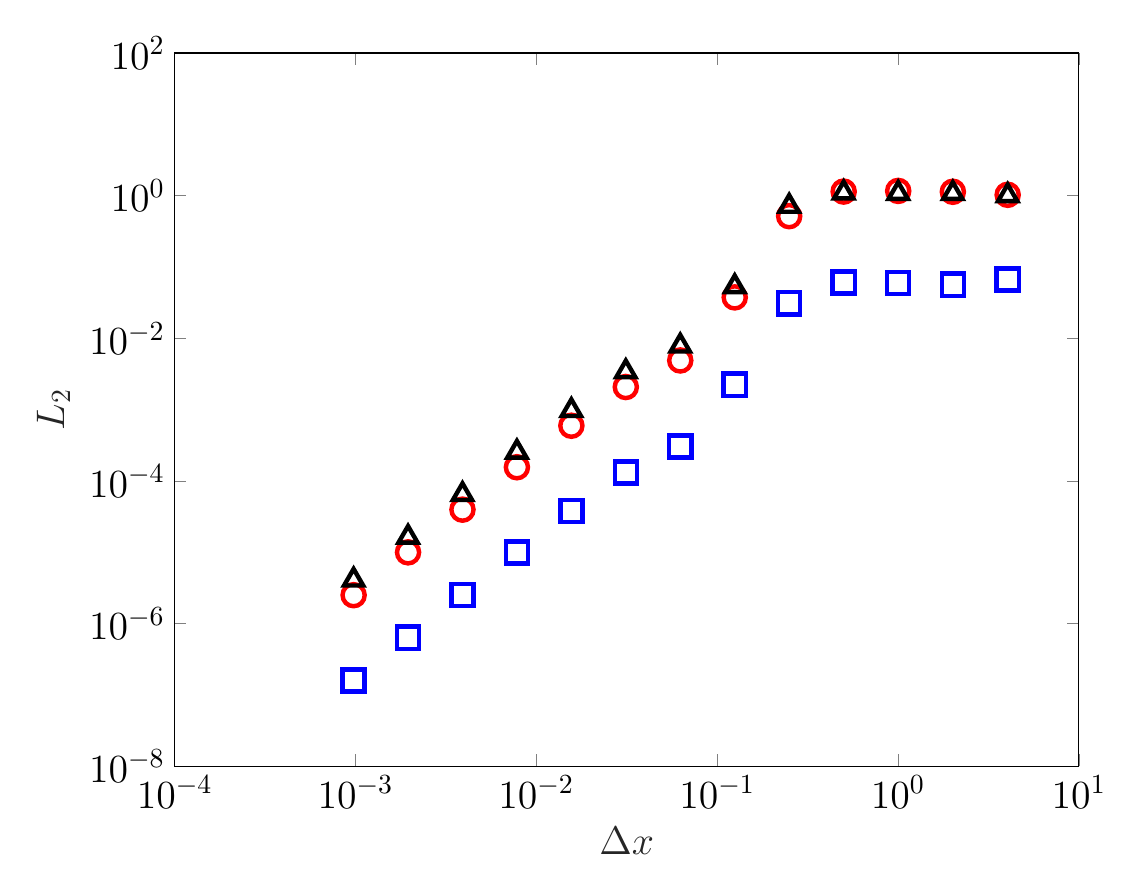
\begin{tikzpicture}
\tikzstyle{every node}=[font=\Large]

\begin{axis}[%
width=4.521in,
height=3.566in,
at={(0.758in,0.481in)},
every axis plot/.append style={ultra thick},
scale only axis,
xmode=log,
xmin=0.0001,
xmax=10,
xtick={0.0001,  0.001,   0.01,    0.1,      1,     10},
xminorticks=false,
xlabel style={font=\color{white!15!black}},
xlabel={\Large $\Delta x$},
ymode=log,
ymin=1e-08,
ymax=100,
ytick={ 1e-08,  1e-06, 0.0001,   0.01,      1,    100},
yminorticks=false,
ylabel style={font=\color{white!15!black}},
ylabel={\Large $L_2$},
axis background/.style={fill=white}
]
 \logLogSlopeTriangle{0.5}{0.2}{0.1}{2}{black};

\addplot [color=blue, draw=none, mark=square, mark size=4pt, mark options={solid, blue}, forget plot]
  table[row sep=crcr]{%
4.04040404040404	0.0667977316044187\\
2.01005025125628	0.0565251008982736\\
1.00250626566416	0.0600244047801842\\
0.500625782227785	0.060369043216863\\
0.250156347717323	0.031027562703989\\
0.125039074710847	0.00223720174663375\\
0.0625097671511174	0.000303213411708855\\
0.0312524415969998	0.00013195585438531\\
0.0156256103754053	3.78678120338089e-05\\
0.00781265259087092	9.90901359842452e-06\\
0.00390628814734519	2.52150220729934e-06\\
0.00195313453678973	6.35217079986901e-07\\
0.000976564884191612	1.59353271500116e-07\\
};
\addplot [color=red, draw=none, mark=o, mark size=4pt, mark options={solid, red}, forget plot]
  table[row sep=crcr]{%
4.04040404040404	1.02894168607817\\
2.01005025125628	1.13471870525711\\
1.00250626566416	1.16651134393852\\
0.500625782227785	1.14209935315627\\
0.250156347717323	0.516295949213657\\
0.125039074710847	0.0375055631709394\\
0.0625097671511174	0.0048956232734942\\
0.0312524415969998	0.00207713643544563\\
0.0156256103754053	0.000595469107815693\\
0.00781265259087092	0.00015580109802979\\
0.00390628814734519	3.96453330936357e-05\\
0.00195313453678973	9.98742874615667e-06\\
0.000976564884191612	2.5054904543415e-06\\
};
\addplot [color=black, draw=none, mark=triangle, mark size=4pt, mark options={solid, black}, forget plot]
  table[row sep=crcr]{%
4.04040404040404	1.00510027333734\\
2.01005025125628	1.07752750295002\\
1.00250626566416	1.07983904140976\\
0.500625782227785	1.09869881739817\\
0.250156347717323	0.712184449316794\\
0.125039074710847	0.05307095900171\\
0.0625097671511174	0.00781225049904385\\
0.0312524415969998	0.00340272133918679\\
0.0156256103754053	0.00097359240010264\\
0.00781265259087092	0.000254452413381455\\
0.00390628814734519	6.47146749585668e-05\\
0.00195313453678973	1.62988208772404e-05\\
0.000976564884191612	4.08829473005837e-06\\
};
%\addplot [color=mycolor1, forget plot]
%  table[row sep=crcr]{%
%4.04040404040404	16.3248648097133\\
%2.01005025125628	4.04030201257544\\
%1.00250626566416	1.0050188126959\\
%0.500625782227785	0.250626173831181\\
%0.250156347717323	0.0625781983032704\\
%0.125039074710847	0.0156347702045448\\
%0.0625097671511174	0.00390747098928691\\
%0.0312524415969998	0.000976715105773881\\
%0.0156256103754053	0.000244159699603973\\
%0.00781265259087092	6.1037540505642e-05\\
%0.00390628814734519	1.52590870900895e-05\\
%0.00195313453678973	3.81473451880083e-06\\
%0.000976564884191612	9.53678973036176e-07\\
%};
\end{axis}
\end{tikzpicture}%
\end{document}
	\caption{$L_2$ norm comparing numerical solution and analytic solution for travelling wave solution with $\beta_1 = \beta_2 = 0$. }
\end{figure}

\begin{figure}
	\centering
	\documentclass[]{standalone}
\usepackage{amsmath}
\usepackage{graphicx}
\usepackage[pdf]{pstricks}
\usepackage{pgfplots}
\pgfplotsset{compat=newest}
\usepgfplotslibrary{fillbetween}
%% the following commands are needed for some matlab2tikz features
\usetikzlibrary{plotmarks}
\usetikzlibrary{arrows.meta}
\usepgfplotslibrary{patchplots}
\usetikzlibrary{decorations.text}
\usetikzlibrary{shapes.multipart}

\newcommand{\logLogSlopeTriangle}[5]
{
	% #1. Relative offset in x direction.
	% #2. Width in x direction, so xA-xB.
	% #3. Relative offset in y direction.
	% #4. Slope d(y)/d(log10(x)).
	% #5. Plot options.
	
	\pgfplotsextra
	{
		\pgfkeysgetvalue{/pgfplots/xmin}{\xmin}
		\pgfkeysgetvalue{/pgfplots/xmax}{\xmax}
		\pgfkeysgetvalue{/pgfplots/ymin}{\ymin}
		\pgfkeysgetvalue{/pgfplots/ymax}{\ymax}
		
		% Calculate auxilliary quantities, in relative sense.
		\pgfmathsetmacro{\xArel}{#1}
		\pgfmathsetmacro{\yArel}{#3}
		\pgfmathsetmacro{\xBrel}{#1-#2}
		\pgfmathsetmacro{\yBrel}{\yArel}
		\pgfmathsetmacro{\xCrel}{\xArel}
		%\pgfmathsetmacro{\yCrel}{ln(\yC/exp(\ymin))/ln(exp(\ymax)/exp(\ymin))} % REPLACE THIS EXPRESSION WITH AN EXPRESSION INDEPENDENT OF \yC TO PREVENT THE 'DIMENSION TOO LARGE' ERROR.
		
		\pgfmathsetmacro{\lnxB}{\xmin*(1-(#1-#2))+\xmax*(#1-#2)} % in [xmin,xmax].
		\pgfmathsetmacro{\lnxA}{\xmin*(1-#1)+\xmax*#1} % in [xmin,xmax].
		\pgfmathsetmacro{\lnyA}{\ymin*(1-#3)+\ymax*#3} % in [ymin,ymax].
		\pgfmathsetmacro{\lnyC}{\lnyA+#4*(\lnxA-\lnxB)}
		\pgfmathsetmacro{\yCrel}{\lnyC-\ymin)/(\ymax-\ymin)} % THE IMPROVED EXPRESSION WITHOUT 'DIMENSION TOO LARGE' ERROR.
		
		% Define coordinates for \draw. MIND THE 'rel axis cs' as opposed to the 'axis cs'.
		\coordinate (A) at (rel axis cs:\xArel,\yArel);
		\coordinate (B) at (rel axis cs:\xBrel,\yBrel);
		\coordinate (C) at (rel axis cs:\xCrel,\yCrel);
		
		% Draw slope triangle.
		\draw[#5]   (A)-- node[pos=0.5,anchor=north] {1}
		(B)-- 
		(C)-- node[pos=0.5,anchor=west] {#4}
		cycle;
	}
}

\begin{document}
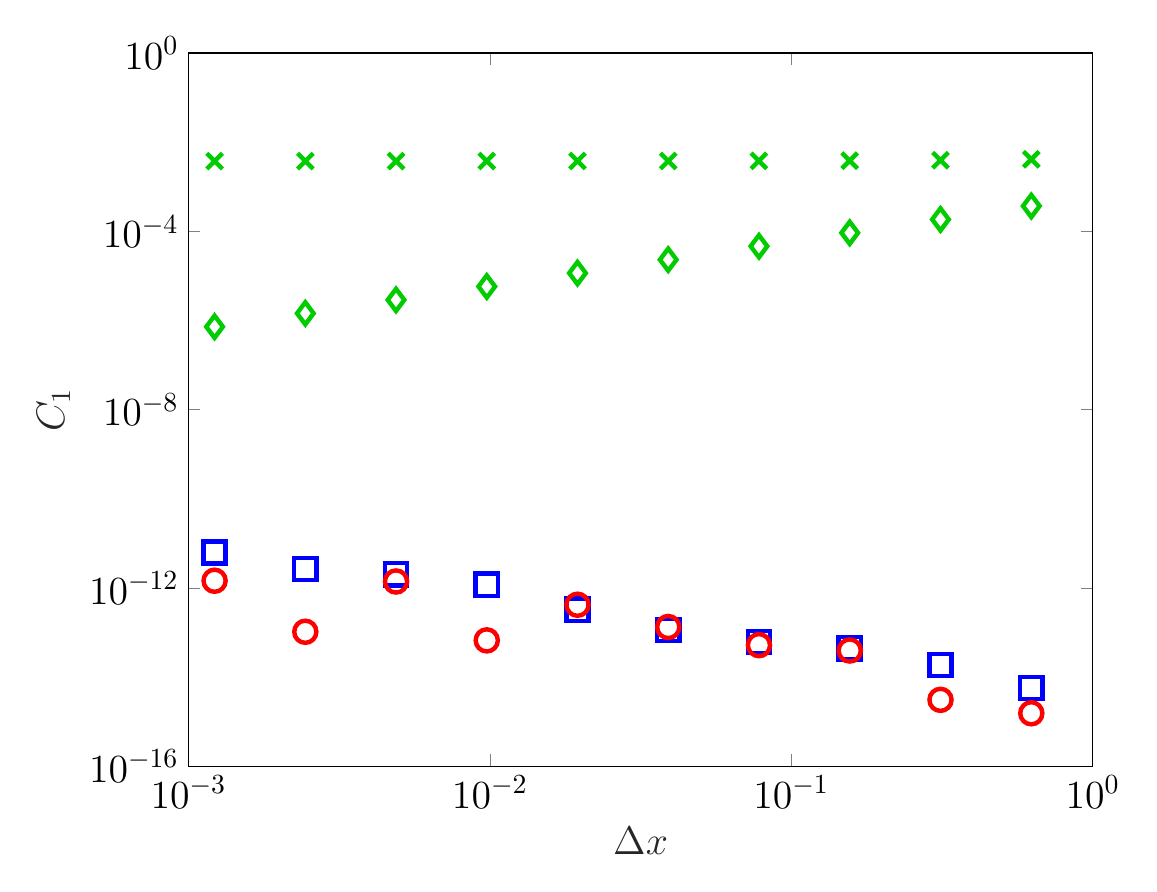
\begin{tikzpicture}
\tikzstyle{every node}=[font=\Large]
\begin{axis}[%
width=4.521in,
height=3.566in,
at={(0.758in,0.481in)},
every axis plot/.append style={ultra thick},
scale only axis,
xmode=log,
xmin=0.001,
xmax=1,
xtick={0.0001,  0.001,   0.01,    0.1,      1,     10},
xminorticks=false,
xlabel style={font=\color{white!15!black}},
xlabel={\Large $\Delta x$},
ymode=log,
ymin=1e-16,
ymax=1,
ytick={ 1e-16,  1e-12,  1e-08, 0.0001,      1},
yminorticks=true,
ylabel style={font=\color{white!15!black}},
ylabel={\Large $C_1$},
axis background/.style={fill=white},
legend style={at={(0.03,0.97)}, anchor=north west, legend cell align=left, align=left, draw=white!15!black}
]

\logLogSlopeTriangle{0.6}{0.5}{0.5}{1}{black};

\addplot [color=blue, draw=none, mark=square, mark size=4pt, mark options={solid, blue}]
  table[row sep=crcr]{%
5.05050505050505	3.56733880835235e-11\\
2.51256281407035	5.12803429349633e-15\\
1.2531328320802	5.29212229594127e-15\\
0.625782227784731	5.75293294483955e-15\\
0.312695434646654	1.84815007742139e-14\\
0.156298843388559	4.43997786684761e-14\\
0.0781372089388967	6.06235062150581e-14\\
0.0390655519962497	1.13374814721569e-13\\
0.0195320129692566	3.24676925344885e-13\\
0.00976581573858864	1.18307791711648e-12\\
0.00488286018418149	2.02072591105225e-12\\
0.00244141817098716	2.68072254395498e-12\\
0.00122070610523951	6.25791459992604e-12\\
};


\addplot [color=red, draw=none, mark=o, mark size=4pt, mark options={solid, red}]
  table[row sep=crcr]{%
5.05050505050505	2.29966242602921e-10\\
2.51256281407035	1.09744947528462e-15\\
1.2531328320802	2.42045514925841e-15\\
0.625782227784731	1.54476055254952e-15\\
0.312695434646654	3.08891006552572e-15\\
0.156298843388559	3.9506271121043e-14\\
0.0781372089388967	5.20946214173407e-14\\
0.0390655519962497	1.32882144892711e-13\\
0.0195320129692566	4.19611018204388e-13\\
0.00976581573858864	6.6662284399639e-14\\
0.00488286018418149	1.39572761789998e-12\\
0.00244141817098716	1.03968198317598e-13\\
0.00122070610523951	1.45092279397927e-12\\
};


%\addplot [color=black, draw=none, mark=triangle, mark size=4pt, mark options={solid, black}]
%  table[row sep=crcr]{%
%5.05050505050505	2.44257645831742e-06\\
%2.51256281407035	1.18170391007563e-06\\
%1.2531328320802	5.81157807324109e-07\\
%0.625782227784731	2.5388600240476e-07\\
%0.312695434646654	1.51556286613131e-07\\
%0.156298843388559	6.36004040868328e-08\\
%0.0781372089388967	3.42368613411178e-08\\
%0.0390655519962497	1.58421274216244e-08\\
%0.0195320129692566	8.62919552106989e-09\\
%0.00976581573858864	4.7145671141896e-09\\
%0.00488286018418149	2.26804766660682e-09\\
%0.00244141817098716	1.18110698751506e-09\\
%0.00122070610523951	5.64680035348884e-10\\
%};


\addplot [color=green, draw=none, mark=x, mark size=4pt, mark options={solid, green!80!black}]
  table[row sep=crcr]{%
5.05050505050505	0.00662111195170816\\
2.51256281407035	0.0052286494667814\\
1.2531328320802	0.00450358876669331\\
0.625782227784731	0.00413064267413027\\
0.312695434646654	0.00394934954073098\\
0.156298843388559	0.00385723425230475\\
0.0781372089388967	0.00381106943412185\\
0.0390655519962497	0.00378839592111398\\
0.0195320129692566	0.00377704290057945\\
0.00976581573858864	0.00377127202990541\\
0.00488286018418149	0.00376838958811927\\
0.00244141817098716	0.00376694735827935\\
0.00122070610523951	0.00376622673914215\\
};


\addplot [color=green, draw=none, only marks, mark=diamond, mark size=4pt, mark options={solid, green!80!black}, forget plot]
  table[row sep=crcr]{%
5.05050505050505	0.00286341532567191\\
2.51256281407035	0.00146591800971105\\
1.2531328320802	0.000738231083097194\\
0.625782227784731	0.00037015118303602\\
0.312695434646654	0.000185092664432067\\
0.156298843388559	9.26437920057067e-05\\
0.0781372089388967	4.63117777600743e-05\\
0.0390655519962497	2.31674191301811e-05\\
0.0195320129692566	1.1578907900003e-05\\
0.00976581573858864	5.78713356834035e-06\\
0.00488286018418149	2.89425127615534e-06\\
0.00244141817098716	1.44679737424634e-06\\
0.00122070610523951	7.23568057607806e-07\\
};

\end{axis}
\end{tikzpicture}%
\end{document}
	\caption{$C$ comparing total amount of conserved quantities in initial conditions and numerical solution for travelling wave solution with $\beta_1 = \beta_2 = 0$. }
\end{figure}


%-----------------------------------------------------
\begin{thebibliography}{99}
%-----------------------------------------------------

\bibitem{Clamond-Dutykh-2018-237}Clamond,~D. and D.~Dutykh, Non-dispersive conservative regularisation of nonlinear shallow water (and isentropic Euler equations), Communications in Nonlinear Science and Numerical Simulation, 55(42), 237-247.

\bibitem{Dutykh-etal-2018-371}Dutykh,~D., M.~Hoefer and D.~Mitsotakis, Soliary wave solutions and their interactions for fully nonlinear water waves with surface tension in the generalized Serre equations, Theoretical and Computational Fluid Dynamics, 32(3), 371-397.

\bibitem{Evans-L-1997} L.C.~Evans, \emph{Partial Differential Equations}, Graduate Studies in Mathematics, Volume 19, American Mathematical Society, New York, (1997).

\bibitem{Harten-A-83-357}  A.~Harten, High resolution schemes for hyperbolic conservation laws, Journal of Computational Physics,  49 (3) (1983) 357-393.

\bibitem{Kurganov-etal-2001-707} A.~Kurganov, S.~Noelle, G.~Petrova, Semidiscrete central-upwind schemes for hyperbolic conservation laws and Hamilton-Jacobi equations, Journal of Scientific Computing, Society for Industrial and Applied Mathematics, 23 (3) (2002) 707-740.

\bibitem{vanLeer-B-1979-101} B.~van~Leer, Towards the ultimate conservative difference scheme, V. A second-order sequel to Godunov's method, Journal of Computational Physics, 32 (1) (1979) 101-136.

\bibitem{Shu-Osher-1988-439} C.W.~Shu, S.~Osher, Efficient implementation of essentially non-oscillatory shock-capturing schemes, Journal of Computational Physics,  77 (2) (1988) 439-471.

\bibitem{Serre-F-1953-857} F.~Serre, Contribution \`{a} l'\'{e}tude des \'{e}coulements permanents et variables dans les canaux, La Houille Blanche, 6 (1953) 830-872.

\bibitem{Zoppou-C-2014} C.~Zoppou, Numerical solution of the one-dimensional and cylindrical Serre equations for rapidly varying free surface flows, Ph.D., Mathematical Sciences Institute, College of Physical and Mathematical Sciences, The Australian National University, (2014).

\bibitem{Zoppou-etal-2017-70}C.~Zoppou, J.~Pitt and S.G.~Roberts, Numerical solution of the fully non-linear weakly dispersive Serre equations for steep gradient flows, Applied Mathematical Modelling, 48, 70-95.

\end{thebibliography}

\end{document} 